\documentclass[twoside]{book}

% Packages required by doxygen
\usepackage{fixltx2e}
\usepackage{calc}
\usepackage{doxygen}
\usepackage[export]{adjustbox} % also loads graphicx
\usepackage{graphicx}
\usepackage[utf8]{inputenc}
\usepackage{makeidx}
\usepackage{multicol}
\usepackage{multirow}
\PassOptionsToPackage{warn}{textcomp}
\usepackage{textcomp}
\usepackage[nointegrals]{wasysym}
\usepackage[table]{xcolor}

% Font selection
\usepackage[T1]{fontenc}
\usepackage[scaled=.90]{helvet}
\usepackage{courier}
\usepackage{amssymb}
\usepackage{sectsty}
\renewcommand{\familydefault}{\sfdefault}
\allsectionsfont{%
  \fontseries{bc}\selectfont%
  \color{darkgray}%
}
\renewcommand{\DoxyLabelFont}{%
  \fontseries{bc}\selectfont%
  \color{darkgray}%
}
\newcommand{\+}{\discretionary{\mbox{\scriptsize$\hookleftarrow$}}{}{}}

% Page & text layout
\usepackage{geometry}
\geometry{%
  a4paper,%
  top=2.5cm,%
  bottom=2.5cm,%
  left=2.5cm,%
  right=2.5cm%
}
\tolerance=750
\hfuzz=15pt
\hbadness=750
\setlength{\emergencystretch}{15pt}
\setlength{\parindent}{0cm}
\setlength{\parskip}{3ex plus 2ex minus 2ex}
\makeatletter
\renewcommand{\paragraph}{%
  \@startsection{paragraph}{4}{0ex}{-1.0ex}{1.0ex}{%
    \normalfont\normalsize\bfseries\SS@parafont%
  }%
}
\renewcommand{\subparagraph}{%
  \@startsection{subparagraph}{5}{0ex}{-1.0ex}{1.0ex}{%
    \normalfont\normalsize\bfseries\SS@subparafont%
  }%
}
\makeatother

% Headers & footers
\usepackage{fancyhdr}
\pagestyle{fancyplain}
\fancyhead[LE]{\fancyplain{}{\bfseries\thepage}}
\fancyhead[CE]{\fancyplain{}{}}
\fancyhead[RE]{\fancyplain{}{\bfseries\leftmark}}
\fancyhead[LO]{\fancyplain{}{\bfseries\rightmark}}
\fancyhead[CO]{\fancyplain{}{}}
\fancyhead[RO]{\fancyplain{}{\bfseries\thepage}}
\fancyfoot[LE]{\fancyplain{}{}}
\fancyfoot[CE]{\fancyplain{}{}}
\fancyfoot[RE]{\fancyplain{}{\bfseries\scriptsize Generated by Doxygen }}
\fancyfoot[LO]{\fancyplain{}{\bfseries\scriptsize Generated by Doxygen }}
\fancyfoot[CO]{\fancyplain{}{}}
\fancyfoot[RO]{\fancyplain{}{}}
\renewcommand{\footrulewidth}{0.4pt}
\renewcommand{\chaptermark}[1]{%
  \markboth{#1}{}%
}
\renewcommand{\sectionmark}[1]{%
  \markright{\thesection\ #1}%
}

% Indices & bibliography
\usepackage{natbib}
\usepackage[titles]{tocloft}
\setcounter{tocdepth}{3}
\setcounter{secnumdepth}{5}
\makeindex

% Hyperlinks (required, but should be loaded last)
\usepackage{ifpdf}
\ifpdf
  \usepackage[pdftex,pagebackref=true]{hyperref}
\else
  \usepackage[ps2pdf,pagebackref=true]{hyperref}
\fi
\hypersetup{%
  colorlinks=true,%
  linkcolor=blue,%
  citecolor=blue,%
  unicode%
}

% Custom commands
\newcommand{\clearemptydoublepage}{%
  \newpage{\pagestyle{empty}\cleardoublepage}%
}

\usepackage{caption}
\captionsetup{labelsep=space,justification=centering,font={bf},singlelinecheck=off,skip=4pt,position=top}

%===== C O N T E N T S =====

\begin{document}

% Titlepage & ToC
\hypersetup{pageanchor=false,
             bookmarksnumbered=true,
             pdfencoding=unicode
            }
\pagenumbering{alph}
\begin{titlepage}
\vspace*{7cm}
\begin{center}%
{\Large terraphast }\\
\vspace*{1cm}
{\large Generated by Doxygen 1.8.13}\\
\end{center}
\end{titlepage}
\clearemptydoublepage
\pagenumbering{roman}
\tableofcontents
\clearemptydoublepage
\pagenumbering{arabic}
\hypersetup{pageanchor=true}

%--- Begin generated contents ---
\chapter{Documentation Home}
\label{index}\hypertarget{index}{}C++ data checker for the existence of terraces in phylogenetic tree space.

\subsection*{Add to this page\+:}


\begin{DoxyItemize}
\item What\textquotesingle{}s the problem we want so solve? What is a terrace?
\item Why is it relevant?
\item How do we solve it?
\item No guarantees for completeness
\item basic code walkthrough
\end{DoxyItemize}

{\bfseries Usage}\+: {\ttfamily terraces/build/release/app $<$nwk file$>$ $<$gene/site file$>$}

Program output states some imput data properties, the species whose leaf edge is used as a new tree root, and the resulting supertree in enhanced newick format. (S\+T\+I\+LL S\+U\+B\+J\+E\+CT TO C\+H\+A\+N\+G\+E!)

{\bfseries Enhanced Newick Format}\+: The resulting supertree representation cann be plain Newick, but can also contain the following two notation enhancements\+:
\begin{DoxyItemize}
\item {\ttfamily \{a,b,c\}} represents any conceivable binary subtree comprising the taxa a, b, and c.
\item {\ttfamily (A$\vert$B,C$\vert$D)} represents any conceivable binary subtree comprising either subtrees A or B on the left, and either subtrees C or D on the right branch.
\end{DoxyItemize}

Both enhancements were chosen such that the result is standard newick format if there\textquotesingle{}s only one possible supertree.

\subsection*{Improvements and Optimizations to the basic approach}

\subsubsection*{Implemented\+:}


\begin{DoxyItemize}
\item We introduced an optional, {\bfseries compressed tree output format}. This format makes printing to terminal faster, since not all possible trees are listed in full detail. See section {\itshape Enhanced Newick Format} above. \mbox{[}\href{https://git.scc.kit.edu/bioinfo2017/terraces/issues/8}{\tt https\+://git.\+scc.\+kit.\+edu/bioinfo2017/terraces/issues/8}\mbox{]}
\item {\bfseries Memory allocation in large blocks}, and managing them with free lists. \mbox{[}\href{https://git.scc.kit.edu/bioinfo2017/terraces/issues/37,}{\tt https\+://git.\+scc.\+kit.\+edu/bioinfo2017/terraces/issues/37,} \href{https://git.scc.kit.edu/bioinfo2017/terraces/issues/13}{\tt https\+://git.\+scc.\+kit.\+edu/bioinfo2017/terraces/issues/13}\mbox{]}
\item {\bfseries Deletion of unnecessary constraints}. \mbox{[}\href{https://git.scc.kit.edu/bioinfo2017/terraces/issues/23}{\tt https\+://git.\+scc.\+kit.\+edu/bioinfo2017/terraces/issues/23}\mbox{]}
\item {\bfseries Improved data structures}\+: We replaced index vectors representing the current leaves by bitvectors with rank support, thus improving space requirements and the efficiency of constraint filtering. The union-\/find data structure could be improved by storing the set ranks in out-\/of-\/bounds indices, thus halving the storage. \mbox{[}\href{https://git.scc.kit.edu/bioinfo2017/terraces/issues/29}{\tt https\+://git.\+scc.\+kit.\+edu/bioinfo2017/terraces/issues/29}\mbox{]}
\item {\bfseries Remap constraints}\+: By removing inner nodes from the constraint numbering, we were able to halve the space requirements of most of our data structures. \mbox{[}\href{https://git.scc.kit.edu/bioinfo2017/terraces/issues/21}{\tt https\+://git.\+scc.\+kit.\+edu/bioinfo2017/terraces/issues/21}\mbox{]}
\item {\bfseries Use specialized bit manipulation instructions}\+: Bipartition iteration and bitvector operations (bit iteration and rank computation) were improved significantly by using specialized C\+PU instructions supported by Compiler intrinsics.
\item {\bfseries Provide a fast terrace check}\+: We discovered that checking for the existence of multiple trees on a terrace can be done without explicitly building any of these trees, thus decreasing the runtime even further.
\item {\bfseries Implemented validation methods}\+: For checking whether the trees generated by our algorithm are indeed distinct and equivalent to the input tree with respect to the missing data, we implemented a fast isomorphy check operating directly on our data structures.
\item Since we wanted to implement different versions of the algorithm, we used a {\bfseries generic enumerator} which relies on callback methods to implement the concrete version of the algorithm (terrace checking, tree counting or multitree construction). This method also allows us to attach {\bfseries logging and status update decorators} to the algorithm to check the internal computations or monitor the progress of the algorithm.
\item Short of support for arbitrary-\/precision math, our implementation is $\ast$$\ast$fully compatible with Visual C++$\ast$$\ast$ in addition to the normal gcc/clang support.
\end{DoxyItemize}

\subsubsection*{Planned\+:}


\begin{DoxyItemize}
\item Enumerate subtrees in {\bfseries parallel}. One challenge would be separation of the workload so that multiple threads have \char`\"{}enough to do\char`\"{}. Another challenge would be the merging of the individual threads\textquotesingle{} results. \mbox{[}\href{https://git.scc.kit.edu/bioinfo2017/terraces/issues/6}{\tt https\+://git.\+scc.\+kit.\+edu/bioinfo2017/terraces/issues/6}\mbox{]}
\item Finding {\bfseries good heuristics} for choosing a subtree into which we want to descend first. Ideally, we\textquotesingle{}d have a nice heuristic that tells us which subtrees and associated constraints probably give us several options to construct a supertree, in which case we can safely answer \char`\"{}yes\char`\"{} to the question \char`\"{}are we on a terrace?\char`\"{}. {\bfseries Ideas}\+: \char`\"{}\+Smallest subtree first\char`\"{}, \char`\"{}\+Least constraints first\char`\"{}. \mbox{[}\href{https://git.scc.kit.edu/bioinfo2017/terraces/issues/3}{\tt https\+://git.\+scc.\+kit.\+edu/bioinfo2017/terraces/issues/3}\mbox{]}
\item ... 
\end{DoxyItemize}
\chapter{Since 1st meeting}
\label{md_Changelog}
\Hypertarget{md_Changelog}
\subsection*{Optimizations }


\begin{DoxyItemize}
\item implement bitvector with rank support
\item use bitvector instead of index vectors for subsets
\item inline lots of often-\/used methods
\item deduplicate constraints
\item remap constraints (removing inner nodes from the numbering)
\item halved union-\/find storage by out-\/of-\/bounds parent trick
\item avoid allocations by reusing old storage
\item some micro-\/optimizations
\end{DoxyItemize}

\subsection*{Fixes and Features }


\begin{DoxyItemize}
\item fast terrace check without traversing the tree to the end
\item fixed subtree computation (problematic input data caused an assertion to fail)
\item fix counting bug (communication problem)
\item don\textquotesingle{}t count incorrectly rooted trees
\item extracted all computations to callback methods
\item implemented logging + stack state decorators
\item implemented isomorphy check
\item Visual C++ compatibility checked with appveyor
\item extracted intrinsics to stay portable 
\end{DoxyItemize}
\chapter{Dependencies}
\label{md_Dependencies}
\Hypertarget{md_Dependencies}
This library has multiple Dependencies

\subsection*{Detailed List }


\begin{DoxyItemize}
\item \href{https://github.com/philsquared/Catch}{\tt Catch}. The header {\ttfamily catch.\+hpp} is supposed to be in the default include-\/path. The framework is avaiable multiple distros under the name {\ttfamily catch}.
\item ...
\end{DoxyItemize}

\subsection*{Copyable List for installation }


\begin{DoxyCode}
catch
\end{DoxyCode}
 
\chapter{A Short Guide to the Codebase}
\label{md_documentation_walkthrough}
\Hypertarget{md_documentation_walkthrough}
This is a short and rather shallow guide to the codebase. Starting from main.\+cpp, you\textquotesingle{}ll see the crucial steps and data structures involved in solving the terrace detection and enumeration problem.

\subsubsection*{0) Interpreting the C\+LI Arguments}

If two file paths are provided, it is assumed that the first path points to the tree file (.nwk) and the second path points to the data file (.data).

If one file path Y/X is provided, it is assumed that the files X.\+nwk and X.\+data are present in the directory Y.

\subsubsection*{1) Parsing the Input Files}

This is done by calling \hyperlink{namespaceterraces_add61915a31828774ee0371d443031c29}{terraces\+::parse\+\_\+nwk} and \hyperlink{namespaceterraces_af52559863b67502f00d68853f50c69af}{terraces\+::parse\+\_\+bitmatrix}. Both throw exceptions, if the input files are not in the right format. If the .data file does not contain a species that possesses all gene sites, this is denoted by a terraces\+::none value in the std\+::pair returned by \hyperlink{namespaceterraces_af52559863b67502f00d68853f50c69af}{terraces\+::parse\+\_\+bitmatrix}. In this case, the current course of action is to exit with error code 1.

\subsubsection*{2) Re-\/\+Rooting the Input Tree}

A call to \hyperlink{namespaceterraces_ae8abab19d1c4a35eb187cd2cf005fe59}{terraces\+::reroot\+\_\+inplace} re-\/roots the given tree at the given species. This is done in-\/place by traversing the input tree from the given species to the original root, and adjusting all edges so that the parent reference of every node points to the node that was traversed before. This procedure has O(tree-\/height) time complexity.

\subsubsection*{3) Extracting Subtrees}

Using an occurence bitmatrix (is gene i present in species j?) and the re-\/rooted tree, all subtrees of this tree are extracted.

\subsubsection*{4) Computing Constraints}

By collecting the left-\/ and rightmost nodes x and y for every inner node i, we establish lowest-\/common-\/ancestor relationships of the form lca(x, y) = i. With this information, we then obtain our constraints of the form lca(x, y) $<$ lca(x, z) which mean that the lowest common ancestor node od x and y is a descendant of the lca of x and z.

\subsubsection*{5) Deduplicating Constaints}

Constraint calculation can result in constraints being found multiple times. \hyperlink{namespaceterraces_a13888c94deeee29c8f5157c9071e3946}{terraces\+::deduplicate\+\_\+constraints} ensures that the given constraints vector contains only unique elements by removing all duplicates.

\subsubsection*{6) Supertree-\/\+Assembly and Output}

Now that we have extracted the constraints from the re-\/rooted version of our tree, we assemble our supertrees according to Constantinescu\textquotesingle{}s Algorithm \mbox{[}C\+S95\mbox{]} which merges sets of nodes so that for each constraint lca(i, j) $<$ lca(k, l), the sets of nodes i and j are merged. This is done for every constraint. In the end, if at least two node sets remain, there\textquotesingle{}s at least one supertree. This gives us the leaves under the two subtrees under our new root\textquotesingle{}s non-\/comprehensive-\/leaf child. In these two subtrees, we then use the constraints to further narrow down the tree\textquotesingle{}s overall structure. Doing so, we can end up with subtress with more than two subtrees and without constraints. In this case, we enumerate all possible subtree topologies.

\subsubsection*{References}

\mbox{[}C\+S95\mbox{]} Mariana Constantinescu and David Sankoff. An efficient algorithm for supertrees. Journal of Classification, 12(1)\+:101–112, 1995. 
\chapter{Namespace Index}
\section{Namespace List}
Here is a list of all namespaces with brief descriptions\+:\begin{DoxyCompactList}
\item\contentsline{section}{\hyperlink{namespaceconvert}{convert} }{\pageref{namespaceconvert}}{}
\item\contentsline{section}{\hyperlink{namespaceterraces}{terraces} }{\pageref{namespaceterraces}}{}
\item\contentsline{section}{\hyperlink{namespaceterraces_1_1bits}{terraces\+::bits} }{\pageref{namespaceterraces_1_1bits}}{}
\item\contentsline{section}{\hyperlink{namespaceterraces_1_1debug}{terraces\+::debug} }{\pageref{namespaceterraces_1_1debug}}{}
\item\contentsline{section}{\hyperlink{namespaceterraces_1_1debug_1_1variants}{terraces\+::debug\+::variants} }{\pageref{namespaceterraces_1_1debug_1_1variants}}{}
\item\contentsline{section}{\hyperlink{namespaceterraces_1_1multitree__impl}{terraces\+::multitree\+\_\+impl} }{\pageref{namespaceterraces_1_1multitree__impl}}{}
\item\contentsline{section}{\hyperlink{namespaceterraces_1_1multitree__nodes}{terraces\+::multitree\+\_\+nodes} }{\pageref{namespaceterraces_1_1multitree__nodes}}{}
\item\contentsline{section}{\hyperlink{namespaceterraces_1_1parsing}{terraces\+::parsing} }{\pageref{namespaceterraces_1_1parsing}}{}
\item\contentsline{section}{\hyperlink{namespaceterraces_1_1tests}{terraces\+::tests} }{\pageref{namespaceterraces_1_1tests}}{}
\item\contentsline{section}{\hyperlink{namespaceterraces_1_1utils}{terraces\+::utils} }{\pageref{namespaceterraces_1_1utils}}{}
\item\contentsline{section}{\hyperlink{namespaceterraces_1_1variants}{terraces\+::variants} }{\pageref{namespaceterraces_1_1variants}}{}
\end{DoxyCompactList}

\chapter{Hierarchical Index}
\section{Class Hierarchy}
This inheritance list is sorted roughly, but not completely, alphabetically\+:\begin{DoxyCompactList}
\item \contentsline{section}{terraces\+:\+:variants\+:\+:abstract\+\_\+callback$<$ Result $>$}{\pageref{classterraces_1_1variants_1_1abstract__callback}}{}
\item \contentsline{section}{terraces\+:\+:variants\+:\+:abstract\+\_\+callback$<$ index $>$}{\pageref{classterraces_1_1variants_1_1abstract__callback}}{}
\begin{DoxyCompactList}
\item \contentsline{section}{terraces\+:\+:variants\+:\+:check\+\_\+callback}{\pageref{classterraces_1_1variants_1_1check__callback}}{}
\end{DoxyCompactList}
\item \contentsline{section}{terraces\+:\+:variants\+:\+:abstract\+\_\+callback$<$ mpz\+\_\+class $>$}{\pageref{classterraces_1_1variants_1_1abstract__callback}}{}
\begin{DoxyCompactList}
\item \contentsline{section}{terraces\+:\+:variants\+:\+:count\+\_\+callback}{\pageref{classterraces_1_1variants_1_1count__callback}}{}
\end{DoxyCompactList}
\item \contentsline{section}{terraces\+:\+:variants\+:\+:abstract\+\_\+callback$<$ multitree\+\_\+node $\ast$$>$}{\pageref{classterraces_1_1variants_1_1abstract__callback}}{}
\begin{DoxyCompactList}
\item \contentsline{section}{terraces\+:\+:variants\+:\+:multitree\+\_\+callback}{\pageref{classterraces_1_1variants_1_1multitree__callback}}{}
\end{DoxyCompactList}
\item \contentsline{section}{terraces\+:\+:multitree\+\_\+nodes\+:\+:alternative\+\_\+array}{\pageref{structterraces_1_1multitree__nodes_1_1alternative__array}}{}
\item \contentsline{section}{terraces\+:\+:utils\+:\+:array\+\_\+deleter}{\pageref{classterraces_1_1utils_1_1array__deleter}}{}
\item \contentsline{section}{terraces\+:\+:tests\+:\+:auto\+\_\+timer}{\pageref{classterraces_1_1tests_1_1auto__timer}}{}
\item \contentsline{section}{terraces\+:\+:basic\+\_\+bitvector$<$ Allocator $>$}{\pageref{classterraces_1_1basic__bitvector}}{}
\item \contentsline{section}{terraces\+:\+:basic\+\_\+bitvector$<$ Alloc $>$}{\pageref{classterraces_1_1basic__bitvector}}{}
\begin{DoxyCompactList}
\item \contentsline{section}{terraces\+:\+:basic\+\_\+ranked\+\_\+bitvector$<$ Alloc $>$}{\pageref{classterraces_1_1basic__ranked__bitvector}}{}
\end{DoxyCompactList}
\item \contentsline{section}{terraces\+:\+:basic\+\_\+bitvector$<$ utils\+:\+:stack\+\_\+allocator$<$ index $>$ $>$}{\pageref{classterraces_1_1basic__bitvector}}{}
\begin{DoxyCompactList}
\item \contentsline{section}{terraces\+:\+:basic\+\_\+ranked\+\_\+bitvector$<$ utils\+:\+:stack\+\_\+allocator$<$ index $>$ $>$}{\pageref{classterraces_1_1basic__ranked__bitvector}}{}
\end{DoxyCompactList}
\item \contentsline{section}{terraces\+:\+:bipartition\+\_\+iterator}{\pageref{classterraces_1_1bipartition__iterator}}{}
\item \contentsline{section}{terraces\+:\+:bitmatrix}{\pageref{classterraces_1_1bitmatrix}}{}
\item \contentsline{section}{terraces\+:\+:bitvector\+\_\+iterator$<$ Alloc $>$}{\pageref{classterraces_1_1bitvector__iterator}}{}
\item Callback\begin{DoxyCompactList}
\item \contentsline{section}{terraces\+:\+:debug\+:\+:variants\+:\+:logging\+\_\+decorator$<$ Callback $>$}{\pageref{classterraces_1_1debug_1_1variants_1_1logging__decorator}}{}
\item \contentsline{section}{terraces\+:\+:debug\+:\+:variants\+:\+:stack\+\_\+state\+\_\+decorator$<$ Callback $>$}{\pageref{classterraces_1_1debug_1_1variants_1_1stack__state__decorator}}{}
\item \contentsline{section}{terraces\+:\+:variants\+:\+:fast\+\_\+check\+\_\+decorator$<$ Callback $>$}{\pageref{classterraces_1_1variants_1_1fast__check__decorator}}{}
\end{DoxyCompactList}
\item \contentsline{section}{terraces\+:\+:utils\+:\+:comma\+\_\+separated\+\_\+mapped\+\_\+output$<$ T1, T2 $>$}{\pageref{structterraces_1_1utils_1_1comma__separated__mapped__output}}{}
\item \contentsline{section}{terraces\+:\+:utils\+:\+:comma\+\_\+separated\+\_\+mapped\+\_\+subset\+\_\+output$<$ T1, T2, T3 $>$}{\pageref{structterraces_1_1utils_1_1comma__separated__mapped__subset__output}}{}
\item \contentsline{section}{terraces\+:\+:utils\+:\+:comma\+\_\+separated\+\_\+output$<$ T $>$}{\pageref{structterraces_1_1utils_1_1comma__separated__output}}{}
\item \contentsline{section}{terraces\+:\+:constraint}{\pageref{structterraces_1_1constraint}}{}
\item \contentsline{section}{terraces\+:\+:counted\+\_\+supertree}{\pageref{structterraces_1_1counted__supertree}}{}
\item std\+:\+:exception\begin{DoxyCompactList}
\item std\+:\+:runtime\+\_\+error\begin{DoxyCompactList}
\item std\+:\+:overflow\+\_\+error\begin{DoxyCompactList}
\item \contentsline{section}{terraces\+:\+:tree\+\_\+count\+\_\+overflow\+\_\+error}{\pageref{classterraces_1_1tree__count__overflow__error}}{}
\end{DoxyCompactList}
\item \contentsline{section}{terraces\+:\+:bad\+\_\+input\+\_\+error}{\pageref{classterraces_1_1bad__input__error}}{}
\item \contentsline{section}{terraces\+:\+:file\+\_\+open\+\_\+error}{\pageref{classterraces_1_1file__open__error}}{}
\item \contentsline{section}{terraces\+:\+:no\+\_\+usable\+\_\+root\+\_\+error}{\pageref{classterraces_1_1no__usable__root__error}}{}
\end{DoxyCompactList}
\end{DoxyCompactList}
\item \contentsline{section}{terraces\+:\+:utils\+:\+:free\+\_\+list}{\pageref{classterraces_1_1utils_1_1free__list}}{}
\item \contentsline{section}{terraces\+:\+:index\+\_\+array\+\_\+view}{\pageref{structterraces_1_1index__array__view}}{}
\item \contentsline{section}{terraces\+:\+:multitree\+\_\+nodes\+:\+:inner\+\_\+node}{\pageref{structterraces_1_1multitree__nodes_1_1inner__node}}{}
\item \contentsline{section}{terraces\+:\+:multitree\+\_\+nodes\+:\+:leaves}{\pageref{structterraces_1_1multitree__nodes_1_1leaves}}{}
\item \contentsline{section}{terraces\+:\+:multitree\+\_\+node}{\pageref{structterraces_1_1multitree__node}}{}
\item \contentsline{section}{terraces\+:\+:utils\+:\+:named\+\_\+output$<$ T2, T3 $>$}{\pageref{structterraces_1_1utils_1_1named__output}}{}
\item \contentsline{section}{terraces\+:\+:newick\+\_\+multitree\+\_\+t}{\pageref{structterraces_1_1newick__multitree__t}}{}
\item \contentsline{section}{terraces\+:\+:newick\+\_\+t}{\pageref{structterraces_1_1newick__t}}{}
\item \contentsline{section}{terraces\+:\+:node}{\pageref{structterraces_1_1node}}{}
\item \contentsline{section}{terraces\+:\+:parsing\+:\+:parser\+\_\+state}{\pageref{structterraces_1_1parsing_1_1parser__state}}{}
\item \contentsline{section}{terraces\+:\+:small\+\_\+bipartition}{\pageref{structterraces_1_1small__bipartition}}{}
\item \contentsline{section}{terraces\+:\+:utils\+:\+:stack\+\_\+allocator$<$ T $>$}{\pageref{classterraces_1_1utils_1_1stack__allocator}}{}
\item \contentsline{section}{terraces\+:\+:utils\+:\+:stack\+\_\+allocator$<$ index $>$}{\pageref{classterraces_1_1utils_1_1stack__allocator}}{}
\item \contentsline{section}{terraces\+:\+:debug\+:\+:variants\+:\+:stack\+\_\+state$<$ Result $>$}{\pageref{structterraces_1_1debug_1_1variants_1_1stack__state}}{}
\item \contentsline{section}{terraces\+:\+:debug\+:\+:variants\+:\+:stack\+\_\+state$<$ result\+\_\+type $>$}{\pageref{structterraces_1_1debug_1_1variants_1_1stack__state}}{}
\item \contentsline{section}{terraces\+:\+:multitree\+\_\+impl\+:\+:storage\+\_\+block$<$ T $>$}{\pageref{classterraces_1_1multitree__impl_1_1storage__block}}{}
\item \contentsline{section}{terraces\+:\+:multitree\+\_\+impl\+:\+:storage\+\_\+block$<$ index $>$}{\pageref{classterraces_1_1multitree__impl_1_1storage__block}}{}
\item \contentsline{section}{terraces\+:\+:multitree\+\_\+impl\+:\+:storage\+\_\+block$<$ terraces\+:\+:multitree\+\_\+node $>$}{\pageref{classterraces_1_1multitree__impl_1_1storage__block}}{}
\item \contentsline{section}{terraces\+:\+:multitree\+\_\+impl\+:\+:storage\+\_\+blocks$<$ T $>$}{\pageref{classterraces_1_1multitree__impl_1_1storage__blocks}}{}
\item \contentsline{section}{terraces\+:\+:multitree\+\_\+impl\+:\+:storage\+\_\+blocks$<$ index $>$}{\pageref{classterraces_1_1multitree__impl_1_1storage__blocks}}{}
\item \contentsline{section}{terraces\+:\+:multitree\+\_\+impl\+:\+:storage\+\_\+blocks$<$ terraces\+:\+:multitree\+\_\+node $>$}{\pageref{classterraces_1_1multitree__impl_1_1storage__blocks}}{}
\item \contentsline{section}{terraces\+:\+:tests\+:\+:timer}{\pageref{classterraces_1_1tests_1_1timer}}{}
\item \contentsline{section}{terraces\+:\+:parsing\+:\+:token}{\pageref{structterraces_1_1parsing_1_1token}}{}
\item \contentsline{section}{terraces\+:\+:tree\+\_\+cursor}{\pageref{classterraces_1_1tree__cursor}}{}
\item \contentsline{section}{terraces\+:\+:tree\+\_\+enumerator$<$ Callback, Parallel $>$}{\pageref{classterraces_1_1tree__enumerator}}{}
\item \contentsline{section}{terraces\+:\+:tree\+\_\+enumerator$<$ Callback $>$}{\pageref{classterraces_1_1tree__enumerator}}{}
\item \contentsline{section}{tree\+\_\+node}{\pageref{structtree__node}}{}
\item \contentsline{section}{terraces\+:\+:tree\+\_\+set}{\pageref{structterraces_1_1tree__set}}{}
\item \contentsline{section}{terraces\+:\+:multitree\+\_\+nodes\+:\+:unconstrained}{\pageref{structterraces_1_1multitree__nodes_1_1unconstrained}}{}
\item \contentsline{section}{terraces\+:\+:multitree\+\_\+nodes\+:\+:unexplored}{\pageref{structterraces_1_1multitree__nodes_1_1unexplored}}{}
\item \contentsline{section}{terraces\+:\+:union\+\_\+find}{\pageref{classterraces_1_1union__find}}{}
\item \contentsline{section}{terraces\+:\+:debug\+:\+:union\+\_\+find\+\_\+iterable\+\_\+set}{\pageref{structterraces_1_1debug_1_1union__find__iterable__set}}{}
\item \contentsline{section}{terraces\+:\+:debug\+:\+:union\+\_\+find\+\_\+iterable\+\_\+sets}{\pageref{structterraces_1_1debug_1_1union__find__iterable__sets}}{}
\item \contentsline{section}{terraces\+:\+:debug\+:\+:union\+\_\+find\+\_\+set\+\_\+iterator}{\pageref{classterraces_1_1debug_1_1union__find__set__iterator}}{}
\item \contentsline{section}{terraces\+:\+:debug\+:\+:union\+\_\+find\+\_\+sets\+\_\+iterator}{\pageref{classterraces_1_1debug_1_1union__find__sets__iterator}}{}
\end{DoxyCompactList}

\chapter{Class Index}
\section{Class List}
Here are the classes, structs, unions and interfaces with brief descriptions\+:\begin{DoxyCompactList}
\item\contentsline{section}{\hyperlink{classterraces_1_1variants_1_1abstract__callback}{terraces\+::variants\+::abstract\+\_\+callback$<$ Result $>$} }{\pageref{classterraces_1_1variants_1_1abstract__callback}}{}
\item\contentsline{section}{\hyperlink{structterraces_1_1multitree__nodes_1_1alternative__array}{terraces\+::multitree\+\_\+nodes\+::alternative\+\_\+array} }{\pageref{structterraces_1_1multitree__nodes_1_1alternative__array}}{}
\item\contentsline{section}{\hyperlink{classterraces_1_1utils_1_1array__deleter}{terraces\+::utils\+::array\+\_\+deleter} }{\pageref{classterraces_1_1utils_1_1array__deleter}}{}
\item\contentsline{section}{\hyperlink{classterraces_1_1tests_1_1auto__timer}{terraces\+::tests\+::auto\+\_\+timer} }{\pageref{classterraces_1_1tests_1_1auto__timer}}{}
\item\contentsline{section}{\hyperlink{classterraces_1_1bad__input__error}{terraces\+::bad\+\_\+input\+\_\+error} }{\pageref{classterraces_1_1bad__input__error}}{}
\item\contentsline{section}{\hyperlink{classterraces_1_1basic__bitvector}{terraces\+::basic\+\_\+bitvector$<$ Allocator $>$} }{\pageref{classterraces_1_1basic__bitvector}}{}
\item\contentsline{section}{\hyperlink{classterraces_1_1basic__ranked__bitvector}{terraces\+::basic\+\_\+ranked\+\_\+bitvector$<$ Alloc $>$} }{\pageref{classterraces_1_1basic__ranked__bitvector}}{}
\item\contentsline{section}{\hyperlink{classterraces_1_1bipartition__iterator}{terraces\+::bipartition\+\_\+iterator} }{\pageref{classterraces_1_1bipartition__iterator}}{}
\item\contentsline{section}{\hyperlink{classterraces_1_1bitmatrix}{terraces\+::bitmatrix} }{\pageref{classterraces_1_1bitmatrix}}{}
\item\contentsline{section}{\hyperlink{classterraces_1_1bitvector__iterator}{terraces\+::bitvector\+\_\+iterator$<$ Alloc $>$} }{\pageref{classterraces_1_1bitvector__iterator}}{}
\item\contentsline{section}{\hyperlink{classterraces_1_1variants_1_1check__callback}{terraces\+::variants\+::check\+\_\+callback} }{\pageref{classterraces_1_1variants_1_1check__callback}}{}
\item\contentsline{section}{\hyperlink{structterraces_1_1utils_1_1comma__separated__mapped__output}{terraces\+::utils\+::comma\+\_\+separated\+\_\+mapped\+\_\+output$<$ T1, T2 $>$} }{\pageref{structterraces_1_1utils_1_1comma__separated__mapped__output}}{}
\item\contentsline{section}{\hyperlink{structterraces_1_1utils_1_1comma__separated__mapped__subset__output}{terraces\+::utils\+::comma\+\_\+separated\+\_\+mapped\+\_\+subset\+\_\+output$<$ T1, T2, T3 $>$} }{\pageref{structterraces_1_1utils_1_1comma__separated__mapped__subset__output}}{}
\item\contentsline{section}{\hyperlink{structterraces_1_1utils_1_1comma__separated__output}{terraces\+::utils\+::comma\+\_\+separated\+\_\+output$<$ T $>$} }{\pageref{structterraces_1_1utils_1_1comma__separated__output}}{}
\item\contentsline{section}{\hyperlink{structterraces_1_1constraint}{terraces\+::constraint} }{\pageref{structterraces_1_1constraint}}{}
\item\contentsline{section}{\hyperlink{classterraces_1_1variants_1_1count__callback}{terraces\+::variants\+::count\+\_\+callback} }{\pageref{classterraces_1_1variants_1_1count__callback}}{}
\item\contentsline{section}{\hyperlink{structterraces_1_1counted__supertree}{terraces\+::counted\+\_\+supertree} }{\pageref{structterraces_1_1counted__supertree}}{}
\item\contentsline{section}{\hyperlink{classterraces_1_1variants_1_1fast__check__decorator}{terraces\+::variants\+::fast\+\_\+check\+\_\+decorator$<$ Callback $>$} }{\pageref{classterraces_1_1variants_1_1fast__check__decorator}}{}
\item\contentsline{section}{\hyperlink{classterraces_1_1file__open__error}{terraces\+::file\+\_\+open\+\_\+error} }{\pageref{classterraces_1_1file__open__error}}{}
\item\contentsline{section}{\hyperlink{classterraces_1_1utils_1_1free__list}{terraces\+::utils\+::free\+\_\+list} }{\pageref{classterraces_1_1utils_1_1free__list}}{}
\item\contentsline{section}{\hyperlink{structterraces_1_1index__array__view}{terraces\+::index\+\_\+array\+\_\+view} }{\pageref{structterraces_1_1index__array__view}}{}
\item\contentsline{section}{\hyperlink{structterraces_1_1multitree__nodes_1_1inner__node}{terraces\+::multitree\+\_\+nodes\+::inner\+\_\+node} }{\pageref{structterraces_1_1multitree__nodes_1_1inner__node}}{}
\item\contentsline{section}{\hyperlink{structinput__data}{input\+\_\+data} }{\pageref{structinput__data}}{}
\item\contentsline{section}{\hyperlink{structterraces_1_1multitree__nodes_1_1leaves}{terraces\+::multitree\+\_\+nodes\+::leaves} }{\pageref{structterraces_1_1multitree__nodes_1_1leaves}}{}
\item\contentsline{section}{\hyperlink{classterraces_1_1debug_1_1variants_1_1logging__decorator}{terraces\+::debug\+::variants\+::logging\+\_\+decorator$<$ Callback $>$} }{\pageref{classterraces_1_1debug_1_1variants_1_1logging__decorator}}{}
\item\contentsline{section}{\hyperlink{structmissingData}{missing\+Data} }{\pageref{structmissingData}}{}
\item\contentsline{section}{\hyperlink{classterraces_1_1variants_1_1multitree__callback}{terraces\+::variants\+::multitree\+\_\+callback} }{\pageref{classterraces_1_1variants_1_1multitree__callback}}{}
\item\contentsline{section}{\hyperlink{structterraces_1_1multitree__node}{terraces\+::multitree\+\_\+node} }{\pageref{structterraces_1_1multitree__node}}{}
\item\contentsline{section}{\hyperlink{structterraces_1_1utils_1_1named__output}{terraces\+::utils\+::named\+\_\+output$<$ T2, T3 $>$} }{\pageref{structterraces_1_1utils_1_1named__output}}{}
\item\contentsline{section}{\hyperlink{structterraces_1_1newick__multitree__t}{terraces\+::newick\+\_\+multitree\+\_\+t} }{\pageref{structterraces_1_1newick__multitree__t}}{}
\item\contentsline{section}{\hyperlink{structterraces_1_1newick__t}{terraces\+::newick\+\_\+t} }{\pageref{structterraces_1_1newick__t}}{}
\item\contentsline{section}{\hyperlink{classterraces_1_1no__usable__root__error}{terraces\+::no\+\_\+usable\+\_\+root\+\_\+error} }{\pageref{classterraces_1_1no__usable__root__error}}{}
\item\contentsline{section}{\hyperlink{structterraces_1_1node}{terraces\+::node} }{\pageref{structterraces_1_1node}}{}
\item\contentsline{section}{\hyperlink{structterraces_1_1parsing_1_1parser__state}{terraces\+::parsing\+::parser\+\_\+state} }{\pageref{structterraces_1_1parsing_1_1parser__state}}{}
\item\contentsline{section}{\hyperlink{structterraces_1_1small__bipartition}{terraces\+::small\+\_\+bipartition} }{\pageref{structterraces_1_1small__bipartition}}{}
\item\contentsline{section}{\hyperlink{classterraces_1_1utils_1_1stack__allocator}{terraces\+::utils\+::stack\+\_\+allocator$<$ T $>$} }{\pageref{classterraces_1_1utils_1_1stack__allocator}}{}
\item\contentsline{section}{\hyperlink{structterraces_1_1debug_1_1variants_1_1stack__state}{terraces\+::debug\+::variants\+::stack\+\_\+state$<$ Result $>$} }{\pageref{structterraces_1_1debug_1_1variants_1_1stack__state}}{}
\item\contentsline{section}{\hyperlink{classterraces_1_1debug_1_1variants_1_1stack__state__decorator}{terraces\+::debug\+::variants\+::stack\+\_\+state\+\_\+decorator$<$ Callback $>$} }{\pageref{classterraces_1_1debug_1_1variants_1_1stack__state__decorator}}{}
\item\contentsline{section}{\hyperlink{classterraces_1_1multitree__impl_1_1storage__block}{terraces\+::multitree\+\_\+impl\+::storage\+\_\+block$<$ T $>$} }{\pageref{classterraces_1_1multitree__impl_1_1storage__block}}{}
\item\contentsline{section}{\hyperlink{classterraces_1_1multitree__impl_1_1storage__blocks}{terraces\+::multitree\+\_\+impl\+::storage\+\_\+blocks$<$ T $>$} }{\pageref{classterraces_1_1multitree__impl_1_1storage__blocks}}{}
\item\contentsline{section}{\hyperlink{classterraces_1_1tests_1_1timer}{terraces\+::tests\+::timer} }{\pageref{classterraces_1_1tests_1_1timer}}{}
\item\contentsline{section}{\hyperlink{structterraces_1_1parsing_1_1token}{terraces\+::parsing\+::token} }{\pageref{structterraces_1_1parsing_1_1token}}{}
\item\contentsline{section}{\hyperlink{classterraces_1_1tree__count__overflow__error}{terraces\+::tree\+\_\+count\+\_\+overflow\+\_\+error} }{\pageref{classterraces_1_1tree__count__overflow__error}}{}
\item\contentsline{section}{\hyperlink{classterraces_1_1tree__cursor}{terraces\+::tree\+\_\+cursor} }{\pageref{classterraces_1_1tree__cursor}}{}
\item\contentsline{section}{\hyperlink{classterraces_1_1tree__enumerator}{terraces\+::tree\+\_\+enumerator$<$ Callback, Parallel $>$} }{\pageref{classterraces_1_1tree__enumerator}}{}
\item\contentsline{section}{\hyperlink{structtree__node}{tree\+\_\+node} }{\pageref{structtree__node}}{}
\item\contentsline{section}{\hyperlink{structterraces_1_1tree__set}{terraces\+::tree\+\_\+set} }{\pageref{structterraces_1_1tree__set}}{}
\item\contentsline{section}{\hyperlink{structterraces_1_1multitree__nodes_1_1unconstrained}{terraces\+::multitree\+\_\+nodes\+::unconstrained} }{\pageref{structterraces_1_1multitree__nodes_1_1unconstrained}}{}
\item\contentsline{section}{\hyperlink{structterraces_1_1multitree__nodes_1_1unexplored}{terraces\+::multitree\+\_\+nodes\+::unexplored} }{\pageref{structterraces_1_1multitree__nodes_1_1unexplored}}{}
\item\contentsline{section}{\hyperlink{classterraces_1_1union__find}{terraces\+::union\+\_\+find} }{\pageref{classterraces_1_1union__find}}{}
\item\contentsline{section}{\hyperlink{structterraces_1_1debug_1_1union__find__iterable__set}{terraces\+::debug\+::union\+\_\+find\+\_\+iterable\+\_\+set} }{\pageref{structterraces_1_1debug_1_1union__find__iterable__set}}{}
\item\contentsline{section}{\hyperlink{structterraces_1_1debug_1_1union__find__iterable__sets}{terraces\+::debug\+::union\+\_\+find\+\_\+iterable\+\_\+sets} }{\pageref{structterraces_1_1debug_1_1union__find__iterable__sets}}{}
\item\contentsline{section}{\hyperlink{classterraces_1_1debug_1_1union__find__set__iterator}{terraces\+::debug\+::union\+\_\+find\+\_\+set\+\_\+iterator} }{\pageref{classterraces_1_1debug_1_1union__find__set__iterator}}{}
\item\contentsline{section}{\hyperlink{classterraces_1_1debug_1_1union__find__sets__iterator}{terraces\+::debug\+::union\+\_\+find\+\_\+sets\+\_\+iterator} }{\pageref{classterraces_1_1debug_1_1union__find__sets__iterator}}{}
\end{DoxyCompactList}

\chapter{File Index}
\section{File List}
Here is a list of all files with brief descriptions\+:\begin{DoxyCompactList}
\item\contentsline{section}{app/\hyperlink{convert_8cpp}{convert.\+cpp} }{\pageref{convert_8cpp}}{}
\item\contentsline{section}{app/\hyperlink{isomorphic_8cpp}{isomorphic.\+cpp} }{\pageref{isomorphic_8cpp}}{}
\item\contentsline{section}{app/\hyperlink{app_2main_8cpp}{main.\+cpp} }{\pageref{app_2main_8cpp}}{}
\item\contentsline{section}{app/\hyperlink{progress-app_8cpp}{progress-\/app.\+cpp} }{\pageref{progress-app_8cpp}}{}
\item\contentsline{section}{app/\hyperlink{reroot_8cpp}{reroot.\+cpp} }{\pageref{reroot_8cpp}}{}
\item\contentsline{section}{app/\hyperlink{site__gen_8cpp}{site\+\_\+gen.\+cpp} }{\pageref{site__gen_8cpp}}{}
\item\contentsline{section}{app/\hyperlink{subtree_8cpp}{subtree.\+cpp} }{\pageref{subtree_8cpp}}{}
\item\contentsline{section}{app/\hyperlink{tree__gen_8cpp}{tree\+\_\+gen.\+cpp} }{\pageref{tree__gen_8cpp}}{}
\item\contentsline{section}{build/debug/\+C\+Make\+Files/\hyperlink{debug_2CMakeFiles_2feature__tests_8c}{feature\+\_\+tests.\+c} }{\pageref{debug_2CMakeFiles_2feature__tests_8c}}{}
\item\contentsline{section}{build/debug/\+C\+Make\+Files/\hyperlink{debug_2CMakeFiles_2feature__tests_8cxx}{feature\+\_\+tests.\+cxx} }{\pageref{debug_2CMakeFiles_2feature__tests_8cxx}}{}
\item\contentsline{section}{build/debug/\+C\+Make\+Files/3.\+7.\+2/\+Compiler\+Id\+C/\hyperlink{debug_2CMakeFiles_23_87_82_2CompilerIdC_2CMakeCCompilerId_8c}{C\+Make\+C\+Compiler\+Id.\+c} }{\pageref{debug_2CMakeFiles_23_87_82_2CompilerIdC_2CMakeCCompilerId_8c}}{}
\item\contentsline{section}{build/debug/\+C\+Make\+Files/3.\+7.\+2/\+Compiler\+Id\+C\+X\+X/\hyperlink{debug_2CMakeFiles_23_87_82_2CompilerIdCXX_2CMakeCXXCompilerId_8cpp}{C\+Make\+C\+X\+X\+Compiler\+Id.\+cpp} }{\pageref{debug_2CMakeFiles_23_87_82_2CompilerIdCXX_2CMakeCXXCompilerId_8cpp}}{}
\item\contentsline{section}{build/release/\+C\+Make\+Files/\hyperlink{release_2CMakeFiles_2feature__tests_8c}{feature\+\_\+tests.\+c} }{\pageref{release_2CMakeFiles_2feature__tests_8c}}{}
\item\contentsline{section}{build/release/\+C\+Make\+Files/\hyperlink{release_2CMakeFiles_2feature__tests_8cxx}{feature\+\_\+tests.\+cxx} }{\pageref{release_2CMakeFiles_2feature__tests_8cxx}}{}
\item\contentsline{section}{build/release/\+C\+Make\+Files/3.\+7.\+2/\+Compiler\+Id\+C/\hyperlink{release_2CMakeFiles_23_87_82_2CompilerIdC_2CMakeCCompilerId_8c}{C\+Make\+C\+Compiler\+Id.\+c} }{\pageref{release_2CMakeFiles_23_87_82_2CompilerIdC_2CMakeCCompilerId_8c}}{}
\item\contentsline{section}{build/release/\+C\+Make\+Files/3.\+7.\+2/\+Compiler\+Id\+C\+X\+X/\hyperlink{release_2CMakeFiles_23_87_82_2CompilerIdCXX_2CMakeCXXCompilerId_8cpp}{C\+Make\+C\+X\+X\+Compiler\+Id.\+cpp} }{\pageref{release_2CMakeFiles_23_87_82_2CompilerIdCXX_2CMakeCXXCompilerId_8cpp}}{}
\item\contentsline{section}{include/terraces/\hyperlink{bitmatrix_8hpp}{bitmatrix.\+hpp} }{\pageref{bitmatrix_8hpp}}{}
\item\contentsline{section}{include/terraces/\hyperlink{constraints_8hpp}{constraints.\+hpp} }{\pageref{constraints_8hpp}}{}
\item\contentsline{section}{include/terraces/\hyperlink{errors_8hpp}{errors.\+hpp} }{\pageref{errors_8hpp}}{}
\item\contentsline{section}{include/terraces/\hyperlink{io__utils_8hpp}{io\+\_\+utils.\+hpp} }{\pageref{io__utils_8hpp}}{}
\item\contentsline{section}{include/terraces/\hyperlink{multitree_8hpp}{multitree.\+hpp} }{\pageref{multitree_8hpp}}{}
\item\contentsline{section}{include/terraces/\hyperlink{parser_8hpp}{parser.\+hpp} }{\pageref{parser_8hpp}}{}
\item\contentsline{section}{include/terraces/\hyperlink{rooting_8hpp}{rooting.\+hpp} }{\pageref{rooting_8hpp}}{}
\item\contentsline{section}{include/terraces/\hyperlink{simple_8hpp}{simple.\+hpp} }{\pageref{simple_8hpp}}{}
\item\contentsline{section}{include/terraces/\hyperlink{subtree__extraction_8hpp}{subtree\+\_\+extraction.\+hpp} }{\pageref{subtree__extraction_8hpp}}{}
\item\contentsline{section}{include/terraces/\hyperlink{supertree_8hpp}{supertree.\+hpp} }{\pageref{supertree_8hpp}}{}
\item\contentsline{section}{include/terraces/\hyperlink{trees_8hpp}{trees.\+hpp} }{\pageref{trees_8hpp}}{}
\item\contentsline{section}{include/terraces/\hyperlink{validation_8hpp}{validation.\+hpp} }{\pageref{validation_8hpp}}{}
\item\contentsline{section}{lib/\hyperlink{lib_2bipartitions_8cpp}{bipartitions.\+cpp} }{\pageref{lib_2bipartitions_8cpp}}{}
\item\contentsline{section}{lib/\hyperlink{bipartitions_8hpp}{bipartitions.\+hpp} }{\pageref{bipartitions_8hpp}}{}
\item\contentsline{section}{lib/\hyperlink{lib_2bitmatrix_8cpp}{bitmatrix.\+cpp} }{\pageref{lib_2bitmatrix_8cpp}}{}
\item\contentsline{section}{lib/\hyperlink{bits_8hpp}{bits.\+hpp} }{\pageref{bits_8hpp}}{}
\item\contentsline{section}{lib/\hyperlink{bitvector_8hpp}{bitvector.\+hpp} }{\pageref{bitvector_8hpp}}{}
\item\contentsline{section}{lib/\hyperlink{lib_2constraints_8cpp}{constraints.\+cpp} }{\pageref{lib_2constraints_8cpp}}{}
\item\contentsline{section}{lib/\hyperlink{multitree_8cpp}{multitree.\+cpp} }{\pageref{multitree_8cpp}}{}
\item\contentsline{section}{lib/\hyperlink{multitree__impl_8hpp}{multitree\+\_\+impl.\+hpp} }{\pageref{multitree__impl_8hpp}}{}
\item\contentsline{section}{lib/\hyperlink{nodes_8cpp}{nodes.\+cpp} }{\pageref{nodes_8cpp}}{}
\item\contentsline{section}{lib/\hyperlink{lib_2parser_8cpp}{parser.\+cpp} }{\pageref{lib_2parser_8cpp}}{}
\item\contentsline{section}{lib/\hyperlink{ranked__bitvector_8hpp}{ranked\+\_\+bitvector.\+hpp} }{\pageref{ranked__bitvector_8hpp}}{}
\item\contentsline{section}{lib/\hyperlink{lib_2rooting_8cpp}{rooting.\+cpp} }{\pageref{lib_2rooting_8cpp}}{}
\item\contentsline{section}{lib/\hyperlink{simple_8cpp}{simple.\+cpp} }{\pageref{simple_8cpp}}{}
\item\contentsline{section}{lib/\hyperlink{stack__allocator_8hpp}{stack\+\_\+allocator.\+hpp} }{\pageref{stack__allocator_8hpp}}{}
\item\contentsline{section}{lib/\hyperlink{lib_2subtree__extraction_8cpp}{subtree\+\_\+extraction.\+cpp} }{\pageref{lib_2subtree__extraction_8cpp}}{}
\item\contentsline{section}{lib/\hyperlink{lib_2supertree_8cpp}{supertree.\+cpp} }{\pageref{lib_2supertree_8cpp}}{}
\item\contentsline{section}{lib/\hyperlink{supertree__enumerator_8hpp}{supertree\+\_\+enumerator.\+hpp} }{\pageref{supertree__enumerator_8hpp}}{}
\item\contentsline{section}{lib/\hyperlink{supertree__helpers_8cpp}{supertree\+\_\+helpers.\+cpp} }{\pageref{supertree__helpers_8cpp}}{}
\item\contentsline{section}{lib/\hyperlink{supertree__helpers_8hpp}{supertree\+\_\+helpers.\+hpp} }{\pageref{supertree__helpers_8hpp}}{}
\item\contentsline{section}{lib/\hyperlink{supertree__variants_8hpp}{supertree\+\_\+variants.\+hpp} }{\pageref{supertree__variants_8hpp}}{}
\item\contentsline{section}{lib/\hyperlink{supertree__variants__debug_8hpp}{supertree\+\_\+variants\+\_\+debug.\+hpp} }{\pageref{supertree__variants__debug_8hpp}}{}
\item\contentsline{section}{lib/\hyperlink{supertree__variants__multitree_8hpp}{supertree\+\_\+variants\+\_\+multitree.\+hpp} }{\pageref{supertree__variants__multitree_8hpp}}{}
\item\contentsline{section}{lib/\hyperlink{lib_2trees_8cpp}{trees.\+cpp} }{\pageref{lib_2trees_8cpp}}{}
\item\contentsline{section}{lib/\hyperlink{unconstrained__enumerator_8hpp}{unconstrained\+\_\+enumerator.\+hpp} }{\pageref{unconstrained__enumerator_8hpp}}{}
\item\contentsline{section}{lib/\hyperlink{lib_2union__find_8cpp}{union\+\_\+find.\+cpp} }{\pageref{lib_2union__find_8cpp}}{}
\item\contentsline{section}{lib/\hyperlink{union__find_8hpp}{union\+\_\+find.\+hpp} }{\pageref{union__find_8hpp}}{}
\item\contentsline{section}{lib/\hyperlink{union__find__debug_8hpp}{union\+\_\+find\+\_\+debug.\+hpp} }{\pageref{union__find__debug_8hpp}}{}
\item\contentsline{section}{lib/\hyperlink{utils_8hpp}{utils.\+hpp} }{\pageref{utils_8hpp}}{}
\item\contentsline{section}{lib/\hyperlink{lib_2validation_8cpp}{validation.\+cpp} }{\pageref{lib_2validation_8cpp}}{}
\item\contentsline{section}{platform/linux/terraces/\hyperlink{linux_2terraces_2intrinsics_8hpp}{intrinsics.\+hpp} }{\pageref{linux_2terraces_2intrinsics_8hpp}}{}
\item\contentsline{section}{platform/windows/\hyperlink{gmpxx_8h}{gmpxx.\+h} }{\pageref{gmpxx_8h}}{}
\item\contentsline{section}{platform/windows/terraces/\hyperlink{windows_2terraces_2intrinsics_8hpp}{intrinsics.\+hpp} }{\pageref{windows_2terraces_2intrinsics_8hpp}}{}
\item\contentsline{section}{scripts/\hyperlink{convert_8py}{convert.\+py} }{\pageref{convert_8py}}{}
\item\contentsline{section}{test/\hyperlink{app_8cpp}{app.\+cpp} }{\pageref{app_8cpp}}{}
\item\contentsline{section}{test/\hyperlink{test_2bipartitions_8cpp}{bipartitions.\+cpp} }{\pageref{test_2bipartitions_8cpp}}{}
\item\contentsline{section}{test/\hyperlink{test_2bitmatrix_8cpp}{bitmatrix.\+cpp} }{\pageref{test_2bitmatrix_8cpp}}{}
\item\contentsline{section}{test/\hyperlink{bits_8cpp}{bits.\+cpp} }{\pageref{bits_8cpp}}{}
\item\contentsline{section}{test/\hyperlink{bitvector_8cpp}{bitvector.\+cpp} }{\pageref{bitvector_8cpp}}{}
\item\contentsline{section}{test/\hyperlink{test_2constraints_8cpp}{constraints.\+cpp} }{\pageref{test_2constraints_8cpp}}{}
\item\contentsline{section}{test/\hyperlink{demo_8cpp}{demo.\+cpp} }{\pageref{demo_8cpp}}{}
\item\contentsline{section}{test/\hyperlink{fast__set_8cpp}{fast\+\_\+set.\+cpp} }{\pageref{fast__set_8cpp}}{}
\item\contentsline{section}{test/\hyperlink{integration_8cpp}{integration.\+cpp} }{\pageref{integration_8cpp}}{}
\item\contentsline{section}{test/\hyperlink{test_2main_8cpp}{main.\+cpp} }{\pageref{test_2main_8cpp}}{}
\item\contentsline{section}{test/\hyperlink{test_2parser_8cpp}{parser.\+cpp} }{\pageref{test_2parser_8cpp}}{}
\item\contentsline{section}{test/\hyperlink{perf__constraints_8cpp}{perf\+\_\+constraints.\+cpp} }{\pageref{perf__constraints_8cpp}}{}
\item\contentsline{section}{test/\hyperlink{performance_8hpp}{performance.\+hpp} }{\pageref{performance_8hpp}}{}
\item\contentsline{section}{test/\hyperlink{test_2rooting_8cpp}{rooting.\+cpp} }{\pageref{test_2rooting_8cpp}}{}
\item\contentsline{section}{test/\hyperlink{stack__allocator_8cpp}{stack\+\_\+allocator.\+cpp} }{\pageref{stack__allocator_8cpp}}{}
\item\contentsline{section}{test/\hyperlink{test_2subtree__extraction_8cpp}{subtree\+\_\+extraction.\+cpp} }{\pageref{test_2subtree__extraction_8cpp}}{}
\item\contentsline{section}{test/\hyperlink{test_2supertree_8cpp}{supertree.\+cpp} }{\pageref{test_2supertree_8cpp}}{}
\item\contentsline{section}{test/\hyperlink{test_2trees_8cpp}{trees.\+cpp} }{\pageref{test_2trees_8cpp}}{}
\item\contentsline{section}{test/\hyperlink{unconstrained__enumerator_8cpp}{unconstrained\+\_\+enumerator.\+cpp} }{\pageref{unconstrained__enumerator_8cpp}}{}
\item\contentsline{section}{test/\hyperlink{test_2union__find_8cpp}{union\+\_\+find.\+cpp} }{\pageref{test_2union__find_8cpp}}{}
\item\contentsline{section}{test/\hyperlink{util_8cpp}{util.\+cpp} }{\pageref{util_8cpp}}{}
\item\contentsline{section}{test/\hyperlink{test_2validation_8cpp}{validation.\+cpp} }{\pageref{test_2validation_8cpp}}{}
\end{DoxyCompactList}

\chapter{Namespace Documentation}
\hypertarget{namespaceconvert}{}\section{convert Namespace Reference}
\label{namespaceconvert}\index{convert@{convert}}
\subsection*{Variables}
\begin{DoxyCompactItemize}
\item 
\hyperlink{namespaceconvert_af8535903aa99b7698550743368e65b24}{parser} = argparse.\+Argument\+Parser(description=\char`\"{}Convert input\+\_\+data.\+h file to input\+\_\+data.\+nwk and input\+\_\+data.\+data\char`\"{})
\item 
\hyperlink{namespaceconvert_ab8cebf608a2f65563b42a9e36d15faea}{help}
\item 
\hyperlink{namespaceconvert_addfed92e768ff6351d23635234c6421f}{args} = parser.\+parse\+\_\+args()
\item 
list \hyperlink{namespaceconvert_ad822cbc3a6f3edbe9992f38b5c089549}{names} = \mbox{[}$\,$\mbox{]}
\item 
\hyperlink{namespaceconvert_a503fc94db74d6869d7c38721a1f90657}{parts} = line.\+split(\textquotesingle{}\char`\"{}\textquotesingle{})
\item 
\hyperlink{namespaceconvert_a86274e201865c2563ac99453b4942754}{content} = \hyperlink{namespaceconvert_a503fc94db74d6869d7c38721a1f90657}{parts}\mbox{[}1\mbox{]}
\item 
\hyperlink{namespaceconvert_a7178e39504bb511cac59b57fd16d1bbd}{begin}
\item 
\hyperlink{namespaceconvert_ac9289d9fbad9c51e7b759f61b260b248}{end}
\end{DoxyCompactItemize}


\subsection{Variable Documentation}
\mbox{\Hypertarget{namespaceconvert_addfed92e768ff6351d23635234c6421f}\label{namespaceconvert_addfed92e768ff6351d23635234c6421f}} 
\index{convert@{convert}!args@{args}}
\index{args@{args}!convert@{convert}}
\subsubsection{\texorpdfstring{args}{args}}
{\footnotesize\ttfamily convert.\+args = parser.\+parse\+\_\+args()}

\mbox{\Hypertarget{namespaceconvert_a7178e39504bb511cac59b57fd16d1bbd}\label{namespaceconvert_a7178e39504bb511cac59b57fd16d1bbd}} 
\index{convert@{convert}!begin@{begin}}
\index{begin@{begin}!convert@{convert}}
\subsubsection{\texorpdfstring{begin}{begin}}
{\footnotesize\ttfamily convert.\+begin}

\mbox{\Hypertarget{namespaceconvert_a86274e201865c2563ac99453b4942754}\label{namespaceconvert_a86274e201865c2563ac99453b4942754}} 
\index{convert@{convert}!content@{content}}
\index{content@{content}!convert@{convert}}
\subsubsection{\texorpdfstring{content}{content}}
{\footnotesize\ttfamily convert.\+content = \hyperlink{namespaceconvert_a503fc94db74d6869d7c38721a1f90657}{parts}\mbox{[}1\mbox{]}}

\mbox{\Hypertarget{namespaceconvert_ac9289d9fbad9c51e7b759f61b260b248}\label{namespaceconvert_ac9289d9fbad9c51e7b759f61b260b248}} 
\index{convert@{convert}!end@{end}}
\index{end@{end}!convert@{convert}}
\subsubsection{\texorpdfstring{end}{end}}
{\footnotesize\ttfamily convert.\+end}

\mbox{\Hypertarget{namespaceconvert_ab8cebf608a2f65563b42a9e36d15faea}\label{namespaceconvert_ab8cebf608a2f65563b42a9e36d15faea}} 
\index{convert@{convert}!help@{help}}
\index{help@{help}!convert@{convert}}
\subsubsection{\texorpdfstring{help}{help}}
{\footnotesize\ttfamily convert.\+help}

\mbox{\Hypertarget{namespaceconvert_ad822cbc3a6f3edbe9992f38b5c089549}\label{namespaceconvert_ad822cbc3a6f3edbe9992f38b5c089549}} 
\index{convert@{convert}!names@{names}}
\index{names@{names}!convert@{convert}}
\subsubsection{\texorpdfstring{names}{names}}
{\footnotesize\ttfamily convert.\+names = \mbox{[}$\,$\mbox{]}}

\mbox{\Hypertarget{namespaceconvert_af8535903aa99b7698550743368e65b24}\label{namespaceconvert_af8535903aa99b7698550743368e65b24}} 
\index{convert@{convert}!parser@{parser}}
\index{parser@{parser}!convert@{convert}}
\subsubsection{\texorpdfstring{parser}{parser}}
{\footnotesize\ttfamily convert.\+parser = argparse.\+Argument\+Parser(description=\char`\"{}Convert input\+\_\+data.\+h file to input\+\_\+data.\+nwk and input\+\_\+data.\+data\char`\"{})}

\mbox{\Hypertarget{namespaceconvert_a503fc94db74d6869d7c38721a1f90657}\label{namespaceconvert_a503fc94db74d6869d7c38721a1f90657}} 
\index{convert@{convert}!parts@{parts}}
\index{parts@{parts}!convert@{convert}}
\subsubsection{\texorpdfstring{parts}{parts}}
{\footnotesize\ttfamily convert.\+parts = line.\+split(\textquotesingle{}\char`\"{}\textquotesingle{})}


\hypertarget{namespaceterraces}{}\section{terraces Namespace Reference}
\label{namespaceterraces}\index{terraces@{terraces}}
\subsection*{Namespaces}
\begin{DoxyCompactItemize}
\item 
 \hyperlink{namespaceterraces_1_1bits}{bits}
\item 
 \hyperlink{namespaceterraces_1_1debug}{debug}
\item 
 \hyperlink{namespaceterraces_1_1multitree__impl}{multitree\+\_\+impl}
\item 
 \hyperlink{namespaceterraces_1_1multitree__nodes}{multitree\+\_\+nodes}
\item 
 \hyperlink{namespaceterraces_1_1parsing}{parsing}
\item 
 \hyperlink{namespaceterraces_1_1tests}{tests}
\item 
 \hyperlink{namespaceterraces_1_1utils}{utils}
\item 
 \hyperlink{namespaceterraces_1_1variants}{variants}
\end{DoxyCompactItemize}
\subsection*{Classes}
\begin{DoxyCompactItemize}
\item 
class \hyperlink{classterraces_1_1bad__input__error}{bad\+\_\+input\+\_\+error}
\item 
class \hyperlink{classterraces_1_1basic__bitvector}{basic\+\_\+bitvector}
\item 
class \hyperlink{classterraces_1_1basic__ranked__bitvector}{basic\+\_\+ranked\+\_\+bitvector}
\item 
class \hyperlink{classterraces_1_1bipartition__iterator}{bipartition\+\_\+iterator}
\item 
class \hyperlink{classterraces_1_1bitmatrix}{bitmatrix}
\item 
class \hyperlink{classterraces_1_1bitvector__iterator}{bitvector\+\_\+iterator}
\item 
struct \hyperlink{structterraces_1_1constraint}{constraint}
\item 
struct \hyperlink{structterraces_1_1counted__supertree}{counted\+\_\+supertree}
\item 
class \hyperlink{classterraces_1_1file__open__error}{file\+\_\+open\+\_\+error}
\item 
struct \hyperlink{structterraces_1_1index__array__view}{index\+\_\+array\+\_\+view}
\item 
struct \hyperlink{structterraces_1_1multitree__node}{multitree\+\_\+node}
\item 
struct \hyperlink{structterraces_1_1newick__multitree__t}{newick\+\_\+multitree\+\_\+t}
\item 
struct \hyperlink{structterraces_1_1newick__t}{newick\+\_\+t}
\item 
class \hyperlink{classterraces_1_1no__usable__root__error}{no\+\_\+usable\+\_\+root\+\_\+error}
\item 
struct \hyperlink{structterraces_1_1node}{node}
\item 
struct \hyperlink{structterraces_1_1small__bipartition}{small\+\_\+bipartition}
\item 
class \hyperlink{classterraces_1_1tree__count__overflow__error}{tree\+\_\+count\+\_\+overflow\+\_\+error}
\item 
class \hyperlink{classterraces_1_1tree__cursor}{tree\+\_\+cursor}
\item 
class \hyperlink{classterraces_1_1tree__enumerator}{tree\+\_\+enumerator}
\item 
struct \hyperlink{structterraces_1_1tree__set}{tree\+\_\+set}
\item 
class \hyperlink{classterraces_1_1union__find}{union\+\_\+find}
\end{DoxyCompactItemize}
\subsection*{Typedefs}
\begin{DoxyCompactItemize}
\item 
using \hyperlink{namespaceterraces_a6f603ffd30ed4d902fce6424492e0581}{constraints} = std\+::vector$<$ \hyperlink{structterraces_1_1constraint}{constraint} $>$
\item 
using \hyperlink{namespaceterraces_adbc33ccb543d1634e96d0eb02e472c77}{index} = std\+::size\+\_\+t
\begin{DoxyCompactList}\small\item\em Our index-\/type. \end{DoxyCompactList}\item 
using \hyperlink{namespaceterraces_a07aaf7feec4a22c6cdefc14c5a81bdd0}{tree} = std\+::vector$<$ \hyperlink{structterraces_1_1node}{node} $>$
\item 
using \hyperlink{namespaceterraces_a4ef0217fe5aed881737d9bc5a8d45dca}{name\+\_\+map} = std\+::vector$<$ std\+::string $>$
\item 
using \hyperlink{namespaceterraces_a148f3e895119c2a72d995caae669e40d}{index\+\_\+map} = std\+::unordered\+\_\+map$<$ std\+::string, \hyperlink{namespaceterraces_adbc33ccb543d1634e96d0eb02e472c77}{index} $>$
\item 
using \hyperlink{namespaceterraces_a1b526fb554dff829f7ad51eb21d5ed06}{bitvector} = \hyperlink{classterraces_1_1basic__bitvector}{basic\+\_\+bitvector}$<$ \hyperlink{classterraces_1_1utils_1_1stack__allocator}{utils\+::stack\+\_\+allocator}$<$ \hyperlink{namespaceterraces_adbc33ccb543d1634e96d0eb02e472c77}{index} $>$ $>$
\item 
using \hyperlink{namespaceterraces_acc45ec9c561024c50ecbce5b6738ba08}{ranked\+\_\+bitvector} = \hyperlink{classterraces_1_1basic__ranked__bitvector}{basic\+\_\+ranked\+\_\+bitvector}$<$ \hyperlink{classterraces_1_1utils_1_1stack__allocator}{utils\+::stack\+\_\+allocator}$<$ \hyperlink{namespaceterraces_adbc33ccb543d1634e96d0eb02e472c77}{index} $>$ $>$
\end{DoxyCompactItemize}
\subsection*{Enumerations}
\begin{DoxyCompactItemize}
\item 
enum \hyperlink{namespaceterraces_ae1e4987c27eddd3b87041a2f0479bcc1}{multitree\+\_\+node\+\_\+type} \{ \newline
\hyperlink{namespaceterraces_ae1e4987c27eddd3b87041a2f0479bcc1a70e35885c895c187b609f94b096e29f1}{multitree\+\_\+node\+\_\+type\+::base\+\_\+single\+\_\+leaf}, 
\hyperlink{namespaceterraces_ae1e4987c27eddd3b87041a2f0479bcc1adfa457b833292690acca0e88b7b6f5c9}{multitree\+\_\+node\+\_\+type\+::base\+\_\+two\+\_\+leaves}, 
\hyperlink{namespaceterraces_ae1e4987c27eddd3b87041a2f0479bcc1a9c3d991ae32ae0f5981317c6cc6df349}{multitree\+\_\+node\+\_\+type\+::base\+\_\+unconstrained}, 
\hyperlink{namespaceterraces_ae1e4987c27eddd3b87041a2f0479bcc1adccfcf9079db20b56ceaa83c0117b85b}{multitree\+\_\+node\+\_\+type\+::inner\+\_\+node}, 
\newline
\hyperlink{namespaceterraces_ae1e4987c27eddd3b87041a2f0479bcc1a3efbbe65015e1cffe03f16adbb19f7db}{multitree\+\_\+node\+\_\+type\+::alternative\+\_\+array}, 
\hyperlink{namespaceterraces_ae1e4987c27eddd3b87041a2f0479bcc1a842481836d8f0854f1e1e50788f5b4be}{multitree\+\_\+node\+\_\+type\+::unexplored}
 \}
\end{DoxyCompactItemize}
\subsection*{Functions}
\begin{DoxyCompactItemize}
\item 
std\+::ostream \& \hyperlink{namespaceterraces_afe895c6224b473a8ac42ee20a43b60dc}{operator$<$$<$} (std\+::ostream \&s, const \hyperlink{structterraces_1_1constraint}{constraint} \&c)
\item 
std\+::ostream \& \hyperlink{namespaceterraces_afda20576b9d2f9c56f3f6d06efc030fd}{operator$<$$<$} (std\+::ostream \&stream, \hyperlink{structterraces_1_1utils_1_1named__output}{utils\+::named\+\_\+output}$<$ \hyperlink{namespaceterraces_a6f603ffd30ed4d902fce6424492e0581}{constraints}, \hyperlink{namespaceterraces_a4ef0217fe5aed881737d9bc5a8d45dca}{name\+\_\+map} $>$)
\item 
\hyperlink{namespaceterraces_a6f603ffd30ed4d902fce6424492e0581}{constraints} \hyperlink{namespaceterraces_adbc8509d9ed99e4e0ef57af54c89e905}{compute\+\_\+constraints} (const std\+::vector$<$ \hyperlink{namespaceterraces_a07aaf7feec4a22c6cdefc14c5a81bdd0}{tree} $>$ \&trees)
\item 
\hyperlink{namespaceterraces_adbc33ccb543d1634e96d0eb02e472c77}{index} \hyperlink{namespaceterraces_a13888c94deeee29c8f5157c9071e3946}{deduplicate\+\_\+constraints} (\hyperlink{namespaceterraces_a6f603ffd30ed4d902fce6424492e0581}{constraints} \&in\+\_\+c)
\item 
std\+::ostream \& \hyperlink{namespaceterraces_ad5d0342efed28b0bd79f604eb73f9b61}{operator$<$$<$} (std\+::ostream \&stream, \hyperlink{structterraces_1_1newick__multitree__t}{newick\+\_\+multitree\+\_\+t} \hyperlink{namespaceterraces_a07aaf7feec4a22c6cdefc14c5a81bdd0}{tree})
\item 
\hyperlink{structterraces_1_1newick__multitree__t}{newick\+\_\+multitree\+\_\+t} \hyperlink{namespaceterraces_ac1f8e7b342ecb4934d77c309c3ac8692}{as\+\_\+newick} (const \hyperlink{structterraces_1_1multitree__node}{multitree\+\_\+node} $\ast$root, const \hyperlink{namespaceterraces_a4ef0217fe5aed881737d9bc5a8d45dca}{name\+\_\+map} \&names)
\item 
\hyperlink{structterraces_1_1tree__set}{tree\+\_\+set} \hyperlink{namespaceterraces_add61915a31828774ee0371d443031c29}{parse\+\_\+nwk} (const std\+::string \&input)
\item 
std\+::pair$<$ \hyperlink{classterraces_1_1bitmatrix}{bitmatrix}, \hyperlink{namespaceterraces_adbc33ccb543d1634e96d0eb02e472c77}{index} $>$ \hyperlink{namespaceterraces_af52559863b67502f00d68853f50c69af}{parse\+\_\+bitmatrix} (std\+::istream \&input, const \hyperlink{namespaceterraces_a148f3e895119c2a72d995caae669e40d}{index\+\_\+map} \&indices, \hyperlink{namespaceterraces_adbc33ccb543d1634e96d0eb02e472c77}{index} tree\+\_\+size)
\item 
void \hyperlink{namespaceterraces_ae8abab19d1c4a35eb187cd2cf005fe59}{reroot\+\_\+inplace} (\hyperlink{namespaceterraces_a07aaf7feec4a22c6cdefc14c5a81bdd0}{tree} \&t, \hyperlink{namespaceterraces_adbc33ccb543d1634e96d0eb02e472c77}{index} root\+\_\+leaf)
\item 
bool \hyperlink{namespaceterraces_a924744ce1ce711e40d0cf722d551e375}{is\+\_\+on\+\_\+terrace} (std\+::istream \&nwk\+\_\+stream, std\+::istream \&matrix\+\_\+stream)
\item 
bool \hyperlink{namespaceterraces_a4e75afae24e5c7fef4f9b22ea3ee9486}{is\+\_\+on\+\_\+terrace} (std\+::istream \&nwk\+\_\+stream, const std\+::string \&matrix\+\_\+string)
\item 
bool \hyperlink{namespaceterraces_aaa1cfc0f0adeee6408adaf1049c24227}{is\+\_\+on\+\_\+terrace} (const std\+::string \&nwk\+\_\+string, std\+::istream \&matrix\+\_\+stream)
\item 
bool \hyperlink{namespaceterraces_a2dd57bda3af31246492ad52438015b42}{is\+\_\+on\+\_\+terrace} (const std\+::string \&nwk\+\_\+string, const std\+::string \&matrix\+\_\+string)
\item 
bool \hyperlink{namespaceterraces_afadd08934abd0d298e2b36c7025e4565}{is\+\_\+on\+\_\+terrace\+\_\+from\+\_\+file} (const std\+::string \&nwk\+\_\+filename, const std\+::string \&matrix\+\_\+filename)
\item 
std\+::uint64\+\_\+t \hyperlink{namespaceterraces_a7ef22320b680e0859629f36e6366095b}{get\+\_\+terrace\+\_\+size} (std\+::istream \&nwk\+\_\+stream, std\+::istream \&matrix\+\_\+stream)
\item 
std\+::uint64\+\_\+t \hyperlink{namespaceterraces_a3d63d1aacb79fba0eec3047276257247}{get\+\_\+terrace\+\_\+size} (std\+::istream \&nwk\+\_\+stream, const std\+::string \&matrix\+\_\+string)
\item 
std\+::uint64\+\_\+t \hyperlink{namespaceterraces_a134fb35cc9c3ade97715eaef710ee458}{get\+\_\+terrace\+\_\+size} (const std\+::string \&nwk\+\_\+string, std\+::istream \&matrix\+\_\+stream)
\item 
std\+::uint64\+\_\+t \hyperlink{namespaceterraces_a42c8925377cdc643dffb08a08cb76c6b}{get\+\_\+terrace\+\_\+size} (const std\+::string \&nwk\+\_\+string, const std\+::string \&matrix\+\_\+string)
\item 
std\+::uint64\+\_\+t \hyperlink{namespaceterraces_a56e02226b324a2c6c7620ed31be10971}{get\+\_\+terrace\+\_\+size\+\_\+from\+\_\+file} (const std\+::string \&nwk\+\_\+filename, const std\+::string \&matrix\+\_\+filename)
\item 
\hyperlink{gmpxx_8h_a4194ba637e08ba88fb6b56747cc0ee6c}{mpz\+\_\+class} \hyperlink{namespaceterraces_aa5f247849fef83931db798d94f3d3208}{get\+\_\+terrace\+\_\+size\+\_\+as\+\_\+bigint} (std\+::istream \&nwk\+\_\+stream, std\+::istream \&matrix\+\_\+stream)
\item 
\hyperlink{gmpxx_8h_a4194ba637e08ba88fb6b56747cc0ee6c}{mpz\+\_\+class} \hyperlink{namespaceterraces_a52729af5c44841c718693508654a4852}{get\+\_\+terrace\+\_\+size\+\_\+as\+\_\+bigint} (std\+::istream \&nwk\+\_\+stream, const std\+::string \&matrix\+\_\+string)
\item 
\hyperlink{gmpxx_8h_a4194ba637e08ba88fb6b56747cc0ee6c}{mpz\+\_\+class} \hyperlink{namespaceterraces_acb1e910e11d185376512e68fa777c02c}{get\+\_\+terrace\+\_\+size\+\_\+as\+\_\+bigint} (const std\+::string \&nwk\+\_\+string, std\+::istream \&matrix\+\_\+stream)
\item 
\hyperlink{gmpxx_8h_a4194ba637e08ba88fb6b56747cc0ee6c}{mpz\+\_\+class} \hyperlink{namespaceterraces_a77a2041cec698021d4513fe8582295d2}{get\+\_\+terrace\+\_\+size\+\_\+as\+\_\+bigint} (const std\+::string \&nwk\+\_\+string, const std\+::string \&matrix\+\_\+string)
\item 
\hyperlink{gmpxx_8h_a4194ba637e08ba88fb6b56747cc0ee6c}{mpz\+\_\+class} \hyperlink{namespaceterraces_a2fd8367ac496d3302518b44ad2804e0a}{get\+\_\+terrace\+\_\+size\+\_\+as\+\_\+bigint\+\_\+from\+\_\+file} (const std\+::string \&nwk\+\_\+filename, const std\+::string \&matrix\+\_\+filename)
\item 
void \hyperlink{namespaceterraces_a8945b2604514ca878a2ba568029f1062}{print\+\_\+terrace} (std\+::istream \&nwk\+\_\+stream, std\+::istream \&matrix\+\_\+stream, std\+::ostream \&out)
\item 
void \hyperlink{namespaceterraces_ae35eb2f7d41b44f45b8bb1623f188fe3}{print\+\_\+terrace} (std\+::istream \&nwk\+\_\+stream, const std\+::string \&matrix\+\_\+string, std\+::ostream \&out)
\item 
void \hyperlink{namespaceterraces_a6b70762dab550c4b63c1fb12a976c79b}{print\+\_\+terrace} (const std\+::string \&nwk\+\_\+string, std\+::istream \&matrix\+\_\+stream, std\+::ostream \&out)
\item 
void \hyperlink{namespaceterraces_abc9fdae9cfcc6334ed6e3a965e0dbd41}{print\+\_\+terrace} (const std\+::string \&nwk\+\_\+string, const std\+::string \&matrix\+\_\+string, std\+::ostream \&out)
\item 
void \hyperlink{namespaceterraces_a8a1db74ca77db1dd2a23a92e8ff05e34}{print\+\_\+terrace\+\_\+from\+\_\+file} (const std\+::string \&nwk\+\_\+filename, const std\+::string \&matrix\+\_\+filename, std\+::ostream \&output)
\item 
std\+::vector$<$ \hyperlink{namespaceterraces_a07aaf7feec4a22c6cdefc14c5a81bdd0}{tree} $>$ \hyperlink{namespaceterraces_a6878b4ce33b96891a13f1336ee330746}{subtrees} (const \hyperlink{namespaceterraces_a07aaf7feec4a22c6cdefc14c5a81bdd0}{tree} \&t, const \hyperlink{classterraces_1_1bitmatrix}{bitmatrix} \&occ)
\item 
\hyperlink{namespaceterraces_adbc33ccb543d1634e96d0eb02e472c77}{index} \hyperlink{namespaceterraces_aa6cd6a7a07d6af5190482a739c575ece}{remap\+\_\+to\+\_\+leaves} (const \hyperlink{namespaceterraces_a07aaf7feec4a22c6cdefc14c5a81bdd0}{tree} \&t, \hyperlink{namespaceterraces_a6f603ffd30ed4d902fce6424492e0581}{constraints} \&c, \hyperlink{namespaceterraces_a4ef0217fe5aed881737d9bc5a8d45dca}{name\+\_\+map} \&names, \hyperlink{namespaceterraces_adbc33ccb543d1634e96d0eb02e472c77}{index} \&root)
\item 
\hyperlink{gmpxx_8h_a4194ba637e08ba88fb6b56747cc0ee6c}{mpz\+\_\+class} \hyperlink{namespaceterraces_a8451b492b27c157a54e8c8b797896c0a}{count\+\_\+supertree} (\hyperlink{namespaceterraces_adbc33ccb543d1634e96d0eb02e472c77}{index} num\+\_\+leaves, const \hyperlink{namespaceterraces_a6f603ffd30ed4d902fce6424492e0581}{constraints} \&\hyperlink{namespaceterraces_a6f603ffd30ed4d902fce6424492e0581}{constraints}, \hyperlink{namespaceterraces_adbc33ccb543d1634e96d0eb02e472c77}{index} root\+\_\+leaf)
\item 
\hyperlink{gmpxx_8h_a4194ba637e08ba88fb6b56747cc0ee6c}{mpz\+\_\+class} \hyperlink{namespaceterraces_af4db64ea1af8673f87af37b1155f2682}{count\+\_\+supertree} (\hyperlink{namespaceterraces_adbc33ccb543d1634e96d0eb02e472c77}{index} num\+\_\+leaves, const \hyperlink{namespaceterraces_a6f603ffd30ed4d902fce6424492e0581}{constraints} \&\hyperlink{namespaceterraces_a6f603ffd30ed4d902fce6424492e0581}{constraints})
\item 
bool \hyperlink{namespaceterraces_aa6c37d0703e1d1f0fec828f851585e0e}{check\+\_\+supertree} (\hyperlink{namespaceterraces_adbc33ccb543d1634e96d0eb02e472c77}{index} num\+\_\+leaves, const \hyperlink{namespaceterraces_a6f603ffd30ed4d902fce6424492e0581}{constraints} \&\hyperlink{namespaceterraces_a6f603ffd30ed4d902fce6424492e0581}{constraints}, \hyperlink{namespaceterraces_adbc33ccb543d1634e96d0eb02e472c77}{index} root\+\_\+leaf)
\item 
bool \hyperlink{namespaceterraces_a1e7ffb28144d80863f1141aa15c58af3}{check\+\_\+supertree} (\hyperlink{namespaceterraces_adbc33ccb543d1634e96d0eb02e472c77}{index} num\+\_\+leaves, const \hyperlink{namespaceterraces_a6f603ffd30ed4d902fce6424492e0581}{constraints} \&\hyperlink{namespaceterraces_a6f603ffd30ed4d902fce6424492e0581}{constraints})
\item 
std\+::ostream \& \hyperlink{namespaceterraces_a734f29a465c2d80d4ee38d00ba2f7460}{operator$<$$<$} (std\+::ostream \&s, const \hyperlink{structterraces_1_1node}{node} \&n)
\item 
std\+::ostream \& \hyperlink{namespaceterraces_a9699b2c445ed0b3ca46836c7d0500817}{operator$<$$<$} (std\+::ostream \&ss, const \hyperlink{namespaceterraces_a07aaf7feec4a22c6cdefc14c5a81bdd0}{tree} \&t)
\item 
\hyperlink{structterraces_1_1newick__t}{newick\+\_\+t} \hyperlink{namespaceterraces_acad20ba1f31addcf2c533824cda625a3}{as\+\_\+newick} (const \hyperlink{namespaceterraces_a07aaf7feec4a22c6cdefc14c5a81bdd0}{tree} \&t, const \hyperlink{namespaceterraces_a4ef0217fe5aed881737d9bc5a8d45dca}{name\+\_\+map} \&names)
\item 
std\+::ostream \& \hyperlink{namespaceterraces_ad3526c917cfcc4424c9a1cac266e6f9f}{operator$<$$<$} (std\+::ostream \&s, \hyperlink{structterraces_1_1newick__t}{newick\+\_\+t} tree\+\_\+pair)
\item 
bool \hyperlink{namespaceterraces_a501de84c86e5d84c979cf4ec3151708e}{is\+\_\+root} (const \hyperlink{structterraces_1_1node}{node} \&n)
\item 
bool \hyperlink{namespaceterraces_a05257bc42db3c5cbed6ef082df709555}{is\+\_\+leaf} (const \hyperlink{structterraces_1_1node}{node} \&n)
\item 
bool \hyperlink{namespaceterraces_a4f378ba2800025b5b70a8647d70c751f}{is\+\_\+rooted\+\_\+tree} (const \hyperlink{namespaceterraces_a07aaf7feec4a22c6cdefc14c5a81bdd0}{tree} \&t)
\item 
bool \hyperlink{namespaceterraces_adec8cca335bd6030520d919ee9d6aa8b}{is\+\_\+valid\+\_\+tree} (const \hyperlink{namespaceterraces_a07aaf7feec4a22c6cdefc14c5a81bdd0}{tree} \&t)
\item 
{\footnotesize template$<$typename Result $>$ }\\Result \hyperlink{namespaceterraces_a3e839fe10a095b681cf4e7ef3ef687b9}{count\+\_\+unrooted\+\_\+trees} (\hyperlink{namespaceterraces_adbc33ccb543d1634e96d0eb02e472c77}{index} num\+\_\+leaves)
\item 
{\footnotesize template$<$typename F $>$ }\\void \hyperlink{namespaceterraces_a479ffe90c01af88c1683e743d417fe1a}{foreach\+\_\+postorder} (const \hyperlink{namespaceterraces_a07aaf7feec4a22c6cdefc14c5a81bdd0}{tree} \&t, F cb)
\item 
{\footnotesize template$<$typename F $>$ }\\void \hyperlink{namespaceterraces_a38d599d41ed134678e30b9cf7b454759}{foreach\+\_\+preorder} (const \hyperlink{namespaceterraces_a07aaf7feec4a22c6cdefc14c5a81bdd0}{tree} \&t, F cb)
\item 
std\+::vector$<$ \hyperlink{namespaceterraces_adbc33ccb543d1634e96d0eb02e472c77}{index} $>$ \hyperlink{namespaceterraces_a24dbd28eb2657b6dd98233b26b20b93f}{preorder} (const \hyperlink{namespaceterraces_a07aaf7feec4a22c6cdefc14c5a81bdd0}{tree} \&t)
\item 
std\+::vector$<$ \hyperlink{namespaceterraces_adbc33ccb543d1634e96d0eb02e472c77}{index} $>$ \hyperlink{namespaceterraces_ac51a269450af323210628bd90b96c694}{postorder} (const \hyperlink{namespaceterraces_a07aaf7feec4a22c6cdefc14c5a81bdd0}{tree} \&t)
\item 
void \hyperlink{namespaceterraces_a07490ad6d9b91f5d4cd609450676516c}{print\+\_\+tree\+\_\+dot\+\_\+unrooted} (const \hyperlink{namespaceterraces_a07aaf7feec4a22c6cdefc14c5a81bdd0}{tree} \&t, const \hyperlink{namespaceterraces_a4ef0217fe5aed881737d9bc5a8d45dca}{name\+\_\+map} \&names, std\+::ostream \&output, std\+::string name\+\_\+prefix=\char`\"{}\char`\"{})
\item 
bool \hyperlink{namespaceterraces_a58682ec06711d5ae85a58aec6d811d31}{is\+\_\+isomorphic} (const \hyperlink{structterraces_1_1tree__set}{tree\+\_\+set} \&fst, const \hyperlink{structterraces_1_1tree__set}{tree\+\_\+set} \&snd)
\item 
std\+::ostream \& \hyperlink{namespaceterraces_a746aa89cd7b3de5dc7dcc7bc90b08e74}{operator$<$$<$} (std\+::ostream \&stream, const \hyperlink{classterraces_1_1bipartition__iterator}{bipartition\+\_\+iterator} \&it)
\item 
{\footnotesize template$<$typename Alloc $>$ }\\\hyperlink{classterraces_1_1basic__bitvector}{basic\+\_\+bitvector}$<$ Alloc $>$ \hyperlink{namespaceterraces_a89a9c3d18566c475960fa9bbe5954049}{full\+\_\+set} (\hyperlink{namespaceterraces_adbc33ccb543d1634e96d0eb02e472c77}{index} size, Alloc a)
\item 
std\+::ostream \& \hyperlink{namespaceterraces_ab0b3ce0b155ae5858d90f33dd51bf489}{print\+\_\+multitree\+\_\+node} (std\+::ostream \&stream, const \hyperlink{structterraces_1_1multitree__node}{multitree\+\_\+node} $\ast$\hyperlink{structterraces_1_1node}{node}, const \hyperlink{namespaceterraces_a4ef0217fe5aed881737d9bc5a8d45dca}{name\+\_\+map} \&names)
\item 
{\footnotesize template$<$typename Alloc $>$ }\\\hyperlink{classterraces_1_1basic__ranked__bitvector}{basic\+\_\+ranked\+\_\+bitvector}$<$ Alloc $>$ \hyperlink{namespaceterraces_a75e78e4205ecb8d8dbd3485c464741fe}{full\+\_\+ranked\+\_\+set} (\hyperlink{namespaceterraces_adbc33ccb543d1634e96d0eb02e472c77}{index} size, Alloc a)
\item 
\hyperlink{namespaceterraces_a1b526fb554dff829f7ad51eb21d5ed06}{bitvector} \hyperlink{namespaceterraces_acece17bacc62c99a66bcc2a69e04f4d1}{filter\+\_\+constraints} (const \hyperlink{namespaceterraces_acc45ec9c561024c50ecbce5b6738ba08}{ranked\+\_\+bitvector} \&leaves, const \hyperlink{namespaceterraces_a1b526fb554dff829f7ad51eb21d5ed06}{bitvector} \&c\+\_\+occ, const \hyperlink{namespaceterraces_a6f603ffd30ed4d902fce6424492e0581}{constraints} \&c, \hyperlink{classterraces_1_1utils_1_1stack__allocator}{utils\+::stack\+\_\+allocator}$<$ \hyperlink{namespaceterraces_adbc33ccb543d1634e96d0eb02e472c77}{index} $>$ a)
\item 
\hyperlink{classterraces_1_1union__find}{union\+\_\+find} \hyperlink{namespaceterraces_a81a42a8b470521357cd73e5b30c2ad7c}{apply\+\_\+constraints} (const \hyperlink{namespaceterraces_acc45ec9c561024c50ecbce5b6738ba08}{ranked\+\_\+bitvector} \&leaves, const \hyperlink{namespaceterraces_a1b526fb554dff829f7ad51eb21d5ed06}{bitvector} \&c\+\_\+occ, const \hyperlink{namespaceterraces_a6f603ffd30ed4d902fce6424492e0581}{constraints} \&c, \hyperlink{classterraces_1_1utils_1_1stack__allocator}{utils\+::stack\+\_\+allocator}$<$ \hyperlink{namespaceterraces_adbc33ccb543d1634e96d0eb02e472c77}{index} $>$ a)
\item 
\hyperlink{namespaceterraces_a6f603ffd30ed4d902fce6424492e0581}{constraints} \hyperlink{namespaceterraces_a13ef284e706bc528df3f04d49e7be607}{map\+\_\+constraints} (const \hyperlink{namespaceterraces_acc45ec9c561024c50ecbce5b6738ba08}{ranked\+\_\+bitvector} \&leaves, const \hyperlink{namespaceterraces_a6f603ffd30ed4d902fce6424492e0581}{constraints} \&cs)
\item 
\hyperlink{namespaceterraces_acc45ec9c561024c50ecbce5b6738ba08}{ranked\+\_\+bitvector} \hyperlink{namespaceterraces_af8d2516221093e7c6f54648e7b2d01bd}{leaf\+\_\+occ} (const \hyperlink{namespaceterraces_a07aaf7feec4a22c6cdefc14c5a81bdd0}{tree} \&\hyperlink{namespaceterraces_a07aaf7feec4a22c6cdefc14c5a81bdd0}{tree}, \hyperlink{classterraces_1_1utils_1_1stack__allocator}{utils\+::stack\+\_\+allocator}$<$ \hyperlink{namespaceterraces_adbc33ccb543d1634e96d0eb02e472c77}{index} $>$ a)
\item 
std\+::vector$<$ \hyperlink{namespaceterraces_a1b526fb554dff829f7ad51eb21d5ed06}{bitvector} $>$ \hyperlink{namespaceterraces_a34db8e988e2845af99b6b228924a5f56}{tree\+\_\+bipartitions} (const \hyperlink{namespaceterraces_a07aaf7feec4a22c6cdefc14c5a81bdd0}{tree} \&t, const std\+::vector$<$ \hyperlink{namespaceterraces_adbc33ccb543d1634e96d0eb02e472c77}{index} $>$ \&mapping, const \hyperlink{namespaceterraces_acc45ec9c561024c50ecbce5b6738ba08}{ranked\+\_\+bitvector} \&leaves, \hyperlink{classterraces_1_1utils_1_1stack__allocator}{utils\+::stack\+\_\+allocator}$<$ \hyperlink{namespaceterraces_adbc33ccb543d1634e96d0eb02e472c77}{index} $>$ alloc)
\end{DoxyCompactItemize}


\subsection{Typedef Documentation}
\mbox{\Hypertarget{namespaceterraces_a1b526fb554dff829f7ad51eb21d5ed06}\label{namespaceterraces_a1b526fb554dff829f7ad51eb21d5ed06}} 
\index{terraces@{terraces}!bitvector@{bitvector}}
\index{bitvector@{bitvector}!terraces@{terraces}}
\subsubsection{\texorpdfstring{bitvector}{bitvector}}
{\footnotesize\ttfamily using \hyperlink{namespaceterraces_a1b526fb554dff829f7ad51eb21d5ed06}{terraces\+::bitvector} = typedef \hyperlink{classterraces_1_1basic__bitvector}{basic\+\_\+bitvector}$<$\hyperlink{classterraces_1_1utils_1_1stack__allocator}{utils\+::stack\+\_\+allocator}$<$\hyperlink{namespaceterraces_adbc33ccb543d1634e96d0eb02e472c77}{index}$>$ $>$}

\mbox{\Hypertarget{namespaceterraces_a6f603ffd30ed4d902fce6424492e0581}\label{namespaceterraces_a6f603ffd30ed4d902fce6424492e0581}} 
\index{terraces@{terraces}!constraints@{constraints}}
\index{constraints@{constraints}!terraces@{terraces}}
\subsubsection{\texorpdfstring{constraints}{constraints}}
{\footnotesize\ttfamily using \hyperlink{namespaceterraces_a6f603ffd30ed4d902fce6424492e0581}{terraces\+::constraints} = typedef std\+::vector$<$\hyperlink{structterraces_1_1constraint}{constraint}$>$}

\mbox{\Hypertarget{namespaceterraces_adbc33ccb543d1634e96d0eb02e472c77}\label{namespaceterraces_adbc33ccb543d1634e96d0eb02e472c77}} 
\index{terraces@{terraces}!index@{index}}
\index{index@{index}!terraces@{terraces}}
\subsubsection{\texorpdfstring{index}{index}}
{\footnotesize\ttfamily using \hyperlink{namespaceterraces_adbc33ccb543d1634e96d0eb02e472c77}{terraces\+::index} = typedef std\+::size\+\_\+t}



Our index-\/type. 

\mbox{\Hypertarget{namespaceterraces_a148f3e895119c2a72d995caae669e40d}\label{namespaceterraces_a148f3e895119c2a72d995caae669e40d}} 
\index{terraces@{terraces}!index\+\_\+map@{index\+\_\+map}}
\index{index\+\_\+map@{index\+\_\+map}!terraces@{terraces}}
\subsubsection{\texorpdfstring{index\+\_\+map}{index\_map}}
{\footnotesize\ttfamily using \hyperlink{namespaceterraces_a148f3e895119c2a72d995caae669e40d}{terraces\+::index\+\_\+map} = typedef std\+::unordered\+\_\+map$<$std\+::string, \hyperlink{namespaceterraces_adbc33ccb543d1634e96d0eb02e472c77}{index}$>$}

\mbox{\Hypertarget{namespaceterraces_a4ef0217fe5aed881737d9bc5a8d45dca}\label{namespaceterraces_a4ef0217fe5aed881737d9bc5a8d45dca}} 
\index{terraces@{terraces}!name\+\_\+map@{name\+\_\+map}}
\index{name\+\_\+map@{name\+\_\+map}!terraces@{terraces}}
\subsubsection{\texorpdfstring{name\+\_\+map}{name\_map}}
{\footnotesize\ttfamily using \hyperlink{namespaceterraces_a4ef0217fe5aed881737d9bc5a8d45dca}{terraces\+::name\+\_\+map} = typedef std\+::vector$<$std\+::string$>$}

\mbox{\Hypertarget{namespaceterraces_acc45ec9c561024c50ecbce5b6738ba08}\label{namespaceterraces_acc45ec9c561024c50ecbce5b6738ba08}} 
\index{terraces@{terraces}!ranked\+\_\+bitvector@{ranked\+\_\+bitvector}}
\index{ranked\+\_\+bitvector@{ranked\+\_\+bitvector}!terraces@{terraces}}
\subsubsection{\texorpdfstring{ranked\+\_\+bitvector}{ranked\_bitvector}}
{\footnotesize\ttfamily using \hyperlink{namespaceterraces_acc45ec9c561024c50ecbce5b6738ba08}{terraces\+::ranked\+\_\+bitvector} = typedef \hyperlink{classterraces_1_1basic__ranked__bitvector}{basic\+\_\+ranked\+\_\+bitvector}$<$\hyperlink{classterraces_1_1utils_1_1stack__allocator}{utils\+::stack\+\_\+allocator}$<$\hyperlink{namespaceterraces_adbc33ccb543d1634e96d0eb02e472c77}{index}$>$ $>$}

\mbox{\Hypertarget{namespaceterraces_a07aaf7feec4a22c6cdefc14c5a81bdd0}\label{namespaceterraces_a07aaf7feec4a22c6cdefc14c5a81bdd0}} 
\index{terraces@{terraces}!tree@{tree}}
\index{tree@{tree}!terraces@{terraces}}
\subsubsection{\texorpdfstring{tree}{tree}}
{\footnotesize\ttfamily using \hyperlink{namespaceterraces_a07aaf7feec4a22c6cdefc14c5a81bdd0}{terraces\+::tree} = typedef std\+::vector$<$\hyperlink{structterraces_1_1node}{node}$>$}



\subsection{Enumeration Type Documentation}
\mbox{\Hypertarget{namespaceterraces_ae1e4987c27eddd3b87041a2f0479bcc1}\label{namespaceterraces_ae1e4987c27eddd3b87041a2f0479bcc1}} 
\index{terraces@{terraces}!multitree\+\_\+node\+\_\+type@{multitree\+\_\+node\+\_\+type}}
\index{multitree\+\_\+node\+\_\+type@{multitree\+\_\+node\+\_\+type}!terraces@{terraces}}
\subsubsection{\texorpdfstring{multitree\+\_\+node\+\_\+type}{multitree\_node\_type}}
{\footnotesize\ttfamily enum \hyperlink{namespaceterraces_ae1e4987c27eddd3b87041a2f0479bcc1}{terraces\+::multitree\+\_\+node\+\_\+type}\hspace{0.3cm}{\ttfamily [strong]}}

\begin{DoxyEnumFields}{Enumerator}
\raisebox{\heightof{T}}[0pt][0pt]{\index{base\+\_\+single\+\_\+leaf@{base\+\_\+single\+\_\+leaf}!terraces@{terraces}}\index{terraces@{terraces}!base\+\_\+single\+\_\+leaf@{base\+\_\+single\+\_\+leaf}}}\mbox{\Hypertarget{namespaceterraces_ae1e4987c27eddd3b87041a2f0479bcc1a70e35885c895c187b609f94b096e29f1}\label{namespaceterraces_ae1e4987c27eddd3b87041a2f0479bcc1a70e35885c895c187b609f94b096e29f1}} 
base\+\_\+single\+\_\+leaf&\\
\hline

\raisebox{\heightof{T}}[0pt][0pt]{\index{base\+\_\+two\+\_\+leaves@{base\+\_\+two\+\_\+leaves}!terraces@{terraces}}\index{terraces@{terraces}!base\+\_\+two\+\_\+leaves@{base\+\_\+two\+\_\+leaves}}}\mbox{\Hypertarget{namespaceterraces_ae1e4987c27eddd3b87041a2f0479bcc1adfa457b833292690acca0e88b7b6f5c9}\label{namespaceterraces_ae1e4987c27eddd3b87041a2f0479bcc1adfa457b833292690acca0e88b7b6f5c9}} 
base\+\_\+two\+\_\+leaves&\\
\hline

\raisebox{\heightof{T}}[0pt][0pt]{\index{base\+\_\+unconstrained@{base\+\_\+unconstrained}!terraces@{terraces}}\index{terraces@{terraces}!base\+\_\+unconstrained@{base\+\_\+unconstrained}}}\mbox{\Hypertarget{namespaceterraces_ae1e4987c27eddd3b87041a2f0479bcc1a9c3d991ae32ae0f5981317c6cc6df349}\label{namespaceterraces_ae1e4987c27eddd3b87041a2f0479bcc1a9c3d991ae32ae0f5981317c6cc6df349}} 
base\+\_\+unconstrained&\\
\hline

\raisebox{\heightof{T}}[0pt][0pt]{\index{inner\+\_\+node@{inner\+\_\+node}!terraces@{terraces}}\index{terraces@{terraces}!inner\+\_\+node@{inner\+\_\+node}}}\mbox{\Hypertarget{namespaceterraces_ae1e4987c27eddd3b87041a2f0479bcc1adccfcf9079db20b56ceaa83c0117b85b}\label{namespaceterraces_ae1e4987c27eddd3b87041a2f0479bcc1adccfcf9079db20b56ceaa83c0117b85b}} 
inner\+\_\+node&\\
\hline

\raisebox{\heightof{T}}[0pt][0pt]{\index{alternative\+\_\+array@{alternative\+\_\+array}!terraces@{terraces}}\index{terraces@{terraces}!alternative\+\_\+array@{alternative\+\_\+array}}}\mbox{\Hypertarget{namespaceterraces_ae1e4987c27eddd3b87041a2f0479bcc1a3efbbe65015e1cffe03f16adbb19f7db}\label{namespaceterraces_ae1e4987c27eddd3b87041a2f0479bcc1a3efbbe65015e1cffe03f16adbb19f7db}} 
alternative\+\_\+array&\\
\hline

\raisebox{\heightof{T}}[0pt][0pt]{\index{unexplored@{unexplored}!terraces@{terraces}}\index{terraces@{terraces}!unexplored@{unexplored}}}\mbox{\Hypertarget{namespaceterraces_ae1e4987c27eddd3b87041a2f0479bcc1a842481836d8f0854f1e1e50788f5b4be}\label{namespaceterraces_ae1e4987c27eddd3b87041a2f0479bcc1a842481836d8f0854f1e1e50788f5b4be}} 
unexplored&\\
\hline

\end{DoxyEnumFields}


\subsection{Function Documentation}
\mbox{\Hypertarget{namespaceterraces_a81a42a8b470521357cd73e5b30c2ad7c}\label{namespaceterraces_a81a42a8b470521357cd73e5b30c2ad7c}} 
\index{terraces@{terraces}!apply\+\_\+constraints@{apply\+\_\+constraints}}
\index{apply\+\_\+constraints@{apply\+\_\+constraints}!terraces@{terraces}}
\subsubsection{\texorpdfstring{apply\+\_\+constraints()}{apply\_constraints()}}
{\footnotesize\ttfamily \hyperlink{classterraces_1_1union__find}{union\+\_\+find} terraces\+::apply\+\_\+constraints (\begin{DoxyParamCaption}\item[{const \hyperlink{namespaceterraces_acc45ec9c561024c50ecbce5b6738ba08}{ranked\+\_\+bitvector} \&}]{leaves,  }\item[{const \hyperlink{namespaceterraces_a1b526fb554dff829f7ad51eb21d5ed06}{bitvector} \&}]{c\+\_\+occ,  }\item[{const \hyperlink{namespaceterraces_a6f603ffd30ed4d902fce6424492e0581}{constraints} \&}]{c,  }\item[{\hyperlink{classterraces_1_1utils_1_1stack__allocator}{utils\+::stack\+\_\+allocator}$<$ \hyperlink{namespaceterraces_adbc33ccb543d1634e96d0eb02e472c77}{index} $>$}]{a }\end{DoxyParamCaption})}

Returns a union-\/find representation of the sets retrieved after applying all constraints from c\+\_\+occ. \mbox{\Hypertarget{namespaceterraces_ac1f8e7b342ecb4934d77c309c3ac8692}\label{namespaceterraces_ac1f8e7b342ecb4934d77c309c3ac8692}} 
\index{terraces@{terraces}!as\+\_\+newick@{as\+\_\+newick}}
\index{as\+\_\+newick@{as\+\_\+newick}!terraces@{terraces}}
\subsubsection{\texorpdfstring{as\+\_\+newick()}{as\_newick()}\hspace{0.1cm}{\footnotesize\ttfamily [1/2]}}
{\footnotesize\ttfamily \hyperlink{structterraces_1_1newick__multitree__t}{newick\+\_\+multitree\+\_\+t} terraces\+::as\+\_\+newick (\begin{DoxyParamCaption}\item[{const \hyperlink{structterraces_1_1multitree__node}{multitree\+\_\+node} $\ast$}]{root,  }\item[{const \hyperlink{namespaceterraces_a4ef0217fe5aed881737d9bc5a8d45dca}{name\+\_\+map} \&}]{names }\end{DoxyParamCaption})\hspace{0.3cm}{\ttfamily [inline]}}

\mbox{\Hypertarget{namespaceterraces_acad20ba1f31addcf2c533824cda625a3}\label{namespaceterraces_acad20ba1f31addcf2c533824cda625a3}} 
\index{terraces@{terraces}!as\+\_\+newick@{as\+\_\+newick}}
\index{as\+\_\+newick@{as\+\_\+newick}!terraces@{terraces}}
\subsubsection{\texorpdfstring{as\+\_\+newick()}{as\_newick()}\hspace{0.1cm}{\footnotesize\ttfamily [2/2]}}
{\footnotesize\ttfamily \hyperlink{structterraces_1_1newick__t}{newick\+\_\+t} terraces\+::as\+\_\+newick (\begin{DoxyParamCaption}\item[{const \hyperlink{namespaceterraces_a07aaf7feec4a22c6cdefc14c5a81bdd0}{tree} \&}]{t,  }\item[{const \hyperlink{namespaceterraces_a4ef0217fe5aed881737d9bc5a8d45dca}{name\+\_\+map} \&}]{names }\end{DoxyParamCaption})\hspace{0.3cm}{\ttfamily [inline]}}

\mbox{\Hypertarget{namespaceterraces_aa6c37d0703e1d1f0fec828f851585e0e}\label{namespaceterraces_aa6c37d0703e1d1f0fec828f851585e0e}} 
\index{terraces@{terraces}!check\+\_\+supertree@{check\+\_\+supertree}}
\index{check\+\_\+supertree@{check\+\_\+supertree}!terraces@{terraces}}
\subsubsection{\texorpdfstring{check\+\_\+supertree()}{check\_supertree()}\hspace{0.1cm}{\footnotesize\ttfamily [1/2]}}
{\footnotesize\ttfamily bool terraces\+::check\+\_\+supertree (\begin{DoxyParamCaption}\item[{\hyperlink{namespaceterraces_adbc33ccb543d1634e96d0eb02e472c77}{index}}]{num\+\_\+leaves,  }\item[{const \hyperlink{namespaceterraces_a6f603ffd30ed4d902fce6424492e0581}{constraints} \&}]{constraints,  }\item[{\hyperlink{namespaceterraces_adbc33ccb543d1634e96d0eb02e472c77}{index}}]{root\+\_\+leaf }\end{DoxyParamCaption})}

Checks if there are at least two trees compatible with the given constraints, while keeping the root fixed. 
\begin{DoxyParams}{Parameters}
{\em num\+\_\+leaves} & The number of leaves of the tree \\
\hline
{\em constraints} & The constraints on the leaves. The constraints must only contain valid leaf indices. \\
\hline
{\em root\+\_\+leaf} & The fixed \textquotesingle{}root leaf\textquotesingle{} which will be placed to the right of the root to avoid isomorphic, differently rooted trees. \\
\hline
\end{DoxyParams}
\begin{DoxyReturn}{Returns}
true iff there are at least two trees compatible with the constraints. 
\end{DoxyReturn}
\mbox{\Hypertarget{namespaceterraces_a1e7ffb28144d80863f1141aa15c58af3}\label{namespaceterraces_a1e7ffb28144d80863f1141aa15c58af3}} 
\index{terraces@{terraces}!check\+\_\+supertree@{check\+\_\+supertree}}
\index{check\+\_\+supertree@{check\+\_\+supertree}!terraces@{terraces}}
\subsubsection{\texorpdfstring{check\+\_\+supertree()}{check\_supertree()}\hspace{0.1cm}{\footnotesize\ttfamily [2/2]}}
{\footnotesize\ttfamily bool terraces\+::check\+\_\+supertree (\begin{DoxyParamCaption}\item[{\hyperlink{namespaceterraces_adbc33ccb543d1634e96d0eb02e472c77}{index}}]{num\+\_\+leaves,  }\item[{const \hyperlink{namespaceterraces_a6f603ffd30ed4d902fce6424492e0581}{constraints} \&}]{constraints }\end{DoxyParamCaption})}

Checks if there are at least two trees compatible with the given constraints. This method might count a tree multiple times if it has a valid isomorphic representation with a different root. 
\begin{DoxyParams}{Parameters}
{\em num\+\_\+leaves} & The number of leaves of the tree \\
\hline
{\em constraints} & The constraints on the leaves. The constraints must only contain valid leaf indices. \\
\hline
\end{DoxyParams}
\begin{DoxyReturn}{Returns}
true iff there are at least two trees compatible with the constraints. 
\end{DoxyReturn}
\mbox{\Hypertarget{namespaceterraces_adbc8509d9ed99e4e0ef57af54c89e905}\label{namespaceterraces_adbc8509d9ed99e4e0ef57af54c89e905}} 
\index{terraces@{terraces}!compute\+\_\+constraints@{compute\+\_\+constraints}}
\index{compute\+\_\+constraints@{compute\+\_\+constraints}!terraces@{terraces}}
\subsubsection{\texorpdfstring{compute\+\_\+constraints()}{compute\_constraints()}}
{\footnotesize\ttfamily \hyperlink{namespaceterraces_a6f603ffd30ed4d902fce6424492e0581}{constraints} terraces\+::compute\+\_\+constraints (\begin{DoxyParamCaption}\item[{const std\+::vector$<$ \hyperlink{namespaceterraces_a07aaf7feec4a22c6cdefc14c5a81bdd0}{tree} $>$ \&}]{trees }\end{DoxyParamCaption})}

\mbox{\Hypertarget{namespaceterraces_a8451b492b27c157a54e8c8b797896c0a}\label{namespaceterraces_a8451b492b27c157a54e8c8b797896c0a}} 
\index{terraces@{terraces}!count\+\_\+supertree@{count\+\_\+supertree}}
\index{count\+\_\+supertree@{count\+\_\+supertree}!terraces@{terraces}}
\subsubsection{\texorpdfstring{count\+\_\+supertree()}{count\_supertree()}\hspace{0.1cm}{\footnotesize\ttfamily [1/2]}}
{\footnotesize\ttfamily \hyperlink{gmpxx_8h_a4194ba637e08ba88fb6b56747cc0ee6c}{mpz\+\_\+class} terraces\+::count\+\_\+supertree (\begin{DoxyParamCaption}\item[{\hyperlink{namespaceterraces_adbc33ccb543d1634e96d0eb02e472c77}{index}}]{num\+\_\+leaves,  }\item[{const \hyperlink{namespaceterraces_a6f603ffd30ed4d902fce6424492e0581}{constraints} \&}]{constraints,  }\item[{\hyperlink{namespaceterraces_adbc33ccb543d1634e96d0eb02e472c77}{index}}]{root\+\_\+leaf }\end{DoxyParamCaption})}

Counts the number of trees compatible with the given constraints, while keeping the root fixed. 
\begin{DoxyParams}{Parameters}
{\em num\+\_\+leaves} & The number of leaves of the tree \\
\hline
{\em constraints} & The constraints on the leaves. The constraints must only contain valid leaf indices. \\
\hline
{\em root\+\_\+leaf} & The fixed \textquotesingle{}root leaf\textquotesingle{} which will be placed to the right of the root to avoid isomorphic, differently rooted trees. \\
\hline
\end{DoxyParams}
\begin{DoxyReturn}{Returns}
the number of trees. 
\end{DoxyReturn}
\mbox{\Hypertarget{namespaceterraces_af4db64ea1af8673f87af37b1155f2682}\label{namespaceterraces_af4db64ea1af8673f87af37b1155f2682}} 
\index{terraces@{terraces}!count\+\_\+supertree@{count\+\_\+supertree}}
\index{count\+\_\+supertree@{count\+\_\+supertree}!terraces@{terraces}}
\subsubsection{\texorpdfstring{count\+\_\+supertree()}{count\_supertree()}\hspace{0.1cm}{\footnotesize\ttfamily [2/2]}}
{\footnotesize\ttfamily \hyperlink{gmpxx_8h_a4194ba637e08ba88fb6b56747cc0ee6c}{mpz\+\_\+class} terraces\+::count\+\_\+supertree (\begin{DoxyParamCaption}\item[{\hyperlink{namespaceterraces_adbc33ccb543d1634e96d0eb02e472c77}{index}}]{num\+\_\+leaves,  }\item[{const \hyperlink{namespaceterraces_a6f603ffd30ed4d902fce6424492e0581}{constraints} \&}]{constraints }\end{DoxyParamCaption})}

Counts the number of trees compatible with the given constraints. This method might count a tree multiple times if it has a valid isomorphic representation with a different root. 
\begin{DoxyParams}{Parameters}
{\em num\+\_\+leaves} & The number of leaves of the tree \\
\hline
{\em constraints} & The constraints on the leaves. The constraints must only contain valid leaf indices. \\
\hline
\end{DoxyParams}
\begin{DoxyReturn}{Returns}
the number of trees. 
\end{DoxyReturn}
\mbox{\Hypertarget{namespaceterraces_a3e839fe10a095b681cf4e7ef3ef687b9}\label{namespaceterraces_a3e839fe10a095b681cf4e7ef3ef687b9}} 
\index{terraces@{terraces}!count\+\_\+unrooted\+\_\+trees@{count\+\_\+unrooted\+\_\+trees}}
\index{count\+\_\+unrooted\+\_\+trees@{count\+\_\+unrooted\+\_\+trees}!terraces@{terraces}}
\subsubsection{\texorpdfstring{count\+\_\+unrooted\+\_\+trees()}{count\_unrooted\_trees()}}
{\footnotesize\ttfamily template$<$typename Result $>$ \\
Result terraces\+::count\+\_\+unrooted\+\_\+trees (\begin{DoxyParamCaption}\item[{\hyperlink{namespaceterraces_adbc33ccb543d1634e96d0eb02e472c77}{index}}]{num\+\_\+leaves }\end{DoxyParamCaption})}

\mbox{\Hypertarget{namespaceterraces_a13888c94deeee29c8f5157c9071e3946}\label{namespaceterraces_a13888c94deeee29c8f5157c9071e3946}} 
\index{terraces@{terraces}!deduplicate\+\_\+constraints@{deduplicate\+\_\+constraints}}
\index{deduplicate\+\_\+constraints@{deduplicate\+\_\+constraints}!terraces@{terraces}}
\subsubsection{\texorpdfstring{deduplicate\+\_\+constraints()}{deduplicate\_constraints()}}
{\footnotesize\ttfamily \hyperlink{namespaceterraces_adbc33ccb543d1634e96d0eb02e472c77}{index} terraces\+::deduplicate\+\_\+constraints (\begin{DoxyParamCaption}\item[{\hyperlink{namespaceterraces_a6f603ffd30ed4d902fce6424492e0581}{constraints} \&}]{in\+\_\+c }\end{DoxyParamCaption})}

\mbox{\Hypertarget{namespaceterraces_acece17bacc62c99a66bcc2a69e04f4d1}\label{namespaceterraces_acece17bacc62c99a66bcc2a69e04f4d1}} 
\index{terraces@{terraces}!filter\+\_\+constraints@{filter\+\_\+constraints}}
\index{filter\+\_\+constraints@{filter\+\_\+constraints}!terraces@{terraces}}
\subsubsection{\texorpdfstring{filter\+\_\+constraints()}{filter\_constraints()}}
{\footnotesize\ttfamily \hyperlink{namespaceterraces_a1b526fb554dff829f7ad51eb21d5ed06}{bitvector} terraces\+::filter\+\_\+constraints (\begin{DoxyParamCaption}\item[{const \hyperlink{namespaceterraces_acc45ec9c561024c50ecbce5b6738ba08}{ranked\+\_\+bitvector} \&}]{leaves,  }\item[{const \hyperlink{namespaceterraces_a1b526fb554dff829f7ad51eb21d5ed06}{bitvector} \&}]{c\+\_\+occ,  }\item[{const \hyperlink{namespaceterraces_a6f603ffd30ed4d902fce6424492e0581}{constraints} \&}]{c,  }\item[{\hyperlink{classterraces_1_1utils_1_1stack__allocator}{utils\+::stack\+\_\+allocator}$<$ \hyperlink{namespaceterraces_adbc33ccb543d1634e96d0eb02e472c77}{index} $>$}]{a }\end{DoxyParamCaption})}

Removes all constraints from c\+\_\+occ that don\textquotesingle{}t lie fully within the leave set. \mbox{\Hypertarget{namespaceterraces_a479ffe90c01af88c1683e743d417fe1a}\label{namespaceterraces_a479ffe90c01af88c1683e743d417fe1a}} 
\index{terraces@{terraces}!foreach\+\_\+postorder@{foreach\+\_\+postorder}}
\index{foreach\+\_\+postorder@{foreach\+\_\+postorder}!terraces@{terraces}}
\subsubsection{\texorpdfstring{foreach\+\_\+postorder()}{foreach\_postorder()}}
{\footnotesize\ttfamily template$<$typename F $>$ \\
void terraces\+::foreach\+\_\+postorder (\begin{DoxyParamCaption}\item[{const \hyperlink{namespaceterraces_a07aaf7feec4a22c6cdefc14c5a81bdd0}{tree} \&}]{t,  }\item[{F}]{cb }\end{DoxyParamCaption})}

Traverses a tree in post-\/order while calling a given callback on every node. \mbox{\Hypertarget{namespaceterraces_a38d599d41ed134678e30b9cf7b454759}\label{namespaceterraces_a38d599d41ed134678e30b9cf7b454759}} 
\index{terraces@{terraces}!foreach\+\_\+preorder@{foreach\+\_\+preorder}}
\index{foreach\+\_\+preorder@{foreach\+\_\+preorder}!terraces@{terraces}}
\subsubsection{\texorpdfstring{foreach\+\_\+preorder()}{foreach\_preorder()}}
{\footnotesize\ttfamily template$<$typename F $>$ \\
void terraces\+::foreach\+\_\+preorder (\begin{DoxyParamCaption}\item[{const \hyperlink{namespaceterraces_a07aaf7feec4a22c6cdefc14c5a81bdd0}{tree} \&}]{t,  }\item[{F}]{cb }\end{DoxyParamCaption})}

\mbox{\Hypertarget{namespaceterraces_a75e78e4205ecb8d8dbd3485c464741fe}\label{namespaceterraces_a75e78e4205ecb8d8dbd3485c464741fe}} 
\index{terraces@{terraces}!full\+\_\+ranked\+\_\+set@{full\+\_\+ranked\+\_\+set}}
\index{full\+\_\+ranked\+\_\+set@{full\+\_\+ranked\+\_\+set}!terraces@{terraces}}
\subsubsection{\texorpdfstring{full\+\_\+ranked\+\_\+set()}{full\_ranked\_set()}}
{\footnotesize\ttfamily template$<$typename Alloc $>$ \\
\hyperlink{classterraces_1_1basic__ranked__bitvector}{basic\+\_\+ranked\+\_\+bitvector}$<$Alloc$>$ terraces\+::full\+\_\+ranked\+\_\+set (\begin{DoxyParamCaption}\item[{\hyperlink{namespaceterraces_adbc33ccb543d1634e96d0eb02e472c77}{index}}]{size,  }\item[{Alloc}]{a }\end{DoxyParamCaption})}

Returns a basic\+\_\+ranked\+\_\+bitvector$<$\+Alloc$>$ containing size elements. \mbox{\Hypertarget{namespaceterraces_a89a9c3d18566c475960fa9bbe5954049}\label{namespaceterraces_a89a9c3d18566c475960fa9bbe5954049}} 
\index{terraces@{terraces}!full\+\_\+set@{full\+\_\+set}}
\index{full\+\_\+set@{full\+\_\+set}!terraces@{terraces}}
\subsubsection{\texorpdfstring{full\+\_\+set()}{full\_set()}}
{\footnotesize\ttfamily template$<$typename Alloc $>$ \\
\hyperlink{classterraces_1_1basic__bitvector}{basic\+\_\+bitvector}$<$Alloc$>$ terraces\+::full\+\_\+set (\begin{DoxyParamCaption}\item[{\hyperlink{namespaceterraces_adbc33ccb543d1634e96d0eb02e472c77}{index}}]{size,  }\item[{Alloc}]{a }\end{DoxyParamCaption})}

Returns a bitvector containing size elements. \mbox{\Hypertarget{namespaceterraces_a7ef22320b680e0859629f36e6366095b}\label{namespaceterraces_a7ef22320b680e0859629f36e6366095b}} 
\index{terraces@{terraces}!get\+\_\+terrace\+\_\+size@{get\+\_\+terrace\+\_\+size}}
\index{get\+\_\+terrace\+\_\+size@{get\+\_\+terrace\+\_\+size}!terraces@{terraces}}
\subsubsection{\texorpdfstring{get\+\_\+terrace\+\_\+size()}{get\_terrace\_size()}\hspace{0.1cm}{\footnotesize\ttfamily [1/4]}}
{\footnotesize\ttfamily std\+::uint64\+\_\+t terraces\+::get\+\_\+terrace\+\_\+size (\begin{DoxyParamCaption}\item[{std\+::istream \&}]{nwk\+\_\+stream,  }\item[{std\+::istream \&}]{matrix\+\_\+stream }\end{DoxyParamCaption})}

Count the number of trees on the terrace. \begin{DoxyReturn}{Returns}
the number of trees on the terrace 
\end{DoxyReturn}
\mbox{\Hypertarget{namespaceterraces_a3d63d1aacb79fba0eec3047276257247}\label{namespaceterraces_a3d63d1aacb79fba0eec3047276257247}} 
\index{terraces@{terraces}!get\+\_\+terrace\+\_\+size@{get\+\_\+terrace\+\_\+size}}
\index{get\+\_\+terrace\+\_\+size@{get\+\_\+terrace\+\_\+size}!terraces@{terraces}}
\subsubsection{\texorpdfstring{get\+\_\+terrace\+\_\+size()}{get\_terrace\_size()}\hspace{0.1cm}{\footnotesize\ttfamily [2/4]}}
{\footnotesize\ttfamily std\+::uint64\+\_\+t terraces\+::get\+\_\+terrace\+\_\+size (\begin{DoxyParamCaption}\item[{std\+::istream \&}]{nwk\+\_\+stream,  }\item[{const std\+::string \&}]{matrix\+\_\+string }\end{DoxyParamCaption})}

\mbox{\Hypertarget{namespaceterraces_a134fb35cc9c3ade97715eaef710ee458}\label{namespaceterraces_a134fb35cc9c3ade97715eaef710ee458}} 
\index{terraces@{terraces}!get\+\_\+terrace\+\_\+size@{get\+\_\+terrace\+\_\+size}}
\index{get\+\_\+terrace\+\_\+size@{get\+\_\+terrace\+\_\+size}!terraces@{terraces}}
\subsubsection{\texorpdfstring{get\+\_\+terrace\+\_\+size()}{get\_terrace\_size()}\hspace{0.1cm}{\footnotesize\ttfamily [3/4]}}
{\footnotesize\ttfamily std\+::uint64\+\_\+t terraces\+::get\+\_\+terrace\+\_\+size (\begin{DoxyParamCaption}\item[{const std\+::string \&}]{nwk\+\_\+string,  }\item[{std\+::istream \&}]{matrix\+\_\+stream }\end{DoxyParamCaption})}

\mbox{\Hypertarget{namespaceterraces_a42c8925377cdc643dffb08a08cb76c6b}\label{namespaceterraces_a42c8925377cdc643dffb08a08cb76c6b}} 
\index{terraces@{terraces}!get\+\_\+terrace\+\_\+size@{get\+\_\+terrace\+\_\+size}}
\index{get\+\_\+terrace\+\_\+size@{get\+\_\+terrace\+\_\+size}!terraces@{terraces}}
\subsubsection{\texorpdfstring{get\+\_\+terrace\+\_\+size()}{get\_terrace\_size()}\hspace{0.1cm}{\footnotesize\ttfamily [4/4]}}
{\footnotesize\ttfamily std\+::uint64\+\_\+t terraces\+::get\+\_\+terrace\+\_\+size (\begin{DoxyParamCaption}\item[{const std\+::string \&}]{nwk\+\_\+string,  }\item[{const std\+::string \&}]{matrix\+\_\+string }\end{DoxyParamCaption})}

\mbox{\Hypertarget{namespaceterraces_aa5f247849fef83931db798d94f3d3208}\label{namespaceterraces_aa5f247849fef83931db798d94f3d3208}} 
\index{terraces@{terraces}!get\+\_\+terrace\+\_\+size\+\_\+as\+\_\+bigint@{get\+\_\+terrace\+\_\+size\+\_\+as\+\_\+bigint}}
\index{get\+\_\+terrace\+\_\+size\+\_\+as\+\_\+bigint@{get\+\_\+terrace\+\_\+size\+\_\+as\+\_\+bigint}!terraces@{terraces}}
\subsubsection{\texorpdfstring{get\+\_\+terrace\+\_\+size\+\_\+as\+\_\+bigint()}{get\_terrace\_size\_as\_bigint()}\hspace{0.1cm}{\footnotesize\ttfamily [1/4]}}
{\footnotesize\ttfamily \hyperlink{gmpxx_8h_a4194ba637e08ba88fb6b56747cc0ee6c}{mpz\+\_\+class} terraces\+::get\+\_\+terrace\+\_\+size\+\_\+as\+\_\+bigint (\begin{DoxyParamCaption}\item[{std\+::istream \&}]{nwk\+\_\+stream,  }\item[{std\+::istream \&}]{matrix\+\_\+stream }\end{DoxyParamCaption})}

\mbox{\Hypertarget{namespaceterraces_a52729af5c44841c718693508654a4852}\label{namespaceterraces_a52729af5c44841c718693508654a4852}} 
\index{terraces@{terraces}!get\+\_\+terrace\+\_\+size\+\_\+as\+\_\+bigint@{get\+\_\+terrace\+\_\+size\+\_\+as\+\_\+bigint}}
\index{get\+\_\+terrace\+\_\+size\+\_\+as\+\_\+bigint@{get\+\_\+terrace\+\_\+size\+\_\+as\+\_\+bigint}!terraces@{terraces}}
\subsubsection{\texorpdfstring{get\+\_\+terrace\+\_\+size\+\_\+as\+\_\+bigint()}{get\_terrace\_size\_as\_bigint()}\hspace{0.1cm}{\footnotesize\ttfamily [2/4]}}
{\footnotesize\ttfamily \hyperlink{gmpxx_8h_a4194ba637e08ba88fb6b56747cc0ee6c}{mpz\+\_\+class} terraces\+::get\+\_\+terrace\+\_\+size\+\_\+as\+\_\+bigint (\begin{DoxyParamCaption}\item[{std\+::istream \&}]{nwk\+\_\+stream,  }\item[{const std\+::string \&}]{matrix\+\_\+string }\end{DoxyParamCaption})}

\mbox{\Hypertarget{namespaceterraces_acb1e910e11d185376512e68fa777c02c}\label{namespaceterraces_acb1e910e11d185376512e68fa777c02c}} 
\index{terraces@{terraces}!get\+\_\+terrace\+\_\+size\+\_\+as\+\_\+bigint@{get\+\_\+terrace\+\_\+size\+\_\+as\+\_\+bigint}}
\index{get\+\_\+terrace\+\_\+size\+\_\+as\+\_\+bigint@{get\+\_\+terrace\+\_\+size\+\_\+as\+\_\+bigint}!terraces@{terraces}}
\subsubsection{\texorpdfstring{get\+\_\+terrace\+\_\+size\+\_\+as\+\_\+bigint()}{get\_terrace\_size\_as\_bigint()}\hspace{0.1cm}{\footnotesize\ttfamily [3/4]}}
{\footnotesize\ttfamily \hyperlink{gmpxx_8h_a4194ba637e08ba88fb6b56747cc0ee6c}{mpz\+\_\+class} terraces\+::get\+\_\+terrace\+\_\+size\+\_\+as\+\_\+bigint (\begin{DoxyParamCaption}\item[{const std\+::string \&}]{nwk\+\_\+string,  }\item[{std\+::istream \&}]{matrix\+\_\+stream }\end{DoxyParamCaption})}

\mbox{\Hypertarget{namespaceterraces_a77a2041cec698021d4513fe8582295d2}\label{namespaceterraces_a77a2041cec698021d4513fe8582295d2}} 
\index{terraces@{terraces}!get\+\_\+terrace\+\_\+size\+\_\+as\+\_\+bigint@{get\+\_\+terrace\+\_\+size\+\_\+as\+\_\+bigint}}
\index{get\+\_\+terrace\+\_\+size\+\_\+as\+\_\+bigint@{get\+\_\+terrace\+\_\+size\+\_\+as\+\_\+bigint}!terraces@{terraces}}
\subsubsection{\texorpdfstring{get\+\_\+terrace\+\_\+size\+\_\+as\+\_\+bigint()}{get\_terrace\_size\_as\_bigint()}\hspace{0.1cm}{\footnotesize\ttfamily [4/4]}}
{\footnotesize\ttfamily \hyperlink{gmpxx_8h_a4194ba637e08ba88fb6b56747cc0ee6c}{mpz\+\_\+class} terraces\+::get\+\_\+terrace\+\_\+size\+\_\+as\+\_\+bigint (\begin{DoxyParamCaption}\item[{const std\+::string \&}]{nwk\+\_\+string,  }\item[{const std\+::string \&}]{matrix\+\_\+string }\end{DoxyParamCaption})}

\mbox{\Hypertarget{namespaceterraces_a2fd8367ac496d3302518b44ad2804e0a}\label{namespaceterraces_a2fd8367ac496d3302518b44ad2804e0a}} 
\index{terraces@{terraces}!get\+\_\+terrace\+\_\+size\+\_\+as\+\_\+bigint\+\_\+from\+\_\+file@{get\+\_\+terrace\+\_\+size\+\_\+as\+\_\+bigint\+\_\+from\+\_\+file}}
\index{get\+\_\+terrace\+\_\+size\+\_\+as\+\_\+bigint\+\_\+from\+\_\+file@{get\+\_\+terrace\+\_\+size\+\_\+as\+\_\+bigint\+\_\+from\+\_\+file}!terraces@{terraces}}
\subsubsection{\texorpdfstring{get\+\_\+terrace\+\_\+size\+\_\+as\+\_\+bigint\+\_\+from\+\_\+file()}{get\_terrace\_size\_as\_bigint\_from\_file()}}
{\footnotesize\ttfamily \hyperlink{gmpxx_8h_a4194ba637e08ba88fb6b56747cc0ee6c}{mpz\+\_\+class} terraces\+::get\+\_\+terrace\+\_\+size\+\_\+as\+\_\+bigint\+\_\+from\+\_\+file (\begin{DoxyParamCaption}\item[{const std\+::string \&}]{nwk\+\_\+filename,  }\item[{const std\+::string \&}]{matrix\+\_\+filename }\end{DoxyParamCaption})}

\mbox{\Hypertarget{namespaceterraces_a56e02226b324a2c6c7620ed31be10971}\label{namespaceterraces_a56e02226b324a2c6c7620ed31be10971}} 
\index{terraces@{terraces}!get\+\_\+terrace\+\_\+size\+\_\+from\+\_\+file@{get\+\_\+terrace\+\_\+size\+\_\+from\+\_\+file}}
\index{get\+\_\+terrace\+\_\+size\+\_\+from\+\_\+file@{get\+\_\+terrace\+\_\+size\+\_\+from\+\_\+file}!terraces@{terraces}}
\subsubsection{\texorpdfstring{get\+\_\+terrace\+\_\+size\+\_\+from\+\_\+file()}{get\_terrace\_size\_from\_file()}}
{\footnotesize\ttfamily std\+::uint64\+\_\+t terraces\+::get\+\_\+terrace\+\_\+size\+\_\+from\+\_\+file (\begin{DoxyParamCaption}\item[{const std\+::string \&}]{nwk\+\_\+filename,  }\item[{const std\+::string \&}]{matrix\+\_\+filename }\end{DoxyParamCaption})}

\mbox{\Hypertarget{namespaceterraces_a58682ec06711d5ae85a58aec6d811d31}\label{namespaceterraces_a58682ec06711d5ae85a58aec6d811d31}} 
\index{terraces@{terraces}!is\+\_\+isomorphic@{is\+\_\+isomorphic}}
\index{is\+\_\+isomorphic@{is\+\_\+isomorphic}!terraces@{terraces}}
\subsubsection{\texorpdfstring{is\+\_\+isomorphic()}{is\_isomorphic()}}
{\footnotesize\ttfamily bool terraces\+::is\+\_\+isomorphic (\begin{DoxyParamCaption}\item[{const \hyperlink{structterraces_1_1tree__set}{tree\+\_\+set} \&}]{fst,  }\item[{const \hyperlink{structterraces_1_1tree__set}{tree\+\_\+set} \&}]{snd }\end{DoxyParamCaption})}

\mbox{\Hypertarget{namespaceterraces_a05257bc42db3c5cbed6ef082df709555}\label{namespaceterraces_a05257bc42db3c5cbed6ef082df709555}} 
\index{terraces@{terraces}!is\+\_\+leaf@{is\+\_\+leaf}}
\index{is\+\_\+leaf@{is\+\_\+leaf}!terraces@{terraces}}
\subsubsection{\texorpdfstring{is\+\_\+leaf()}{is\_leaf()}}
{\footnotesize\ttfamily bool terraces\+::is\+\_\+leaf (\begin{DoxyParamCaption}\item[{const \hyperlink{structterraces_1_1node}{node} \&}]{n }\end{DoxyParamCaption})\hspace{0.3cm}{\ttfamily [inline]}}

Returns whether a node is a leaf. \mbox{\Hypertarget{namespaceterraces_a924744ce1ce711e40d0cf722d551e375}\label{namespaceterraces_a924744ce1ce711e40d0cf722d551e375}} 
\index{terraces@{terraces}!is\+\_\+on\+\_\+terrace@{is\+\_\+on\+\_\+terrace}}
\index{is\+\_\+on\+\_\+terrace@{is\+\_\+on\+\_\+terrace}!terraces@{terraces}}
\subsubsection{\texorpdfstring{is\+\_\+on\+\_\+terrace()}{is\_on\_terrace()}\hspace{0.1cm}{\footnotesize\ttfamily [1/4]}}
{\footnotesize\ttfamily bool terraces\+::is\+\_\+on\+\_\+terrace (\begin{DoxyParamCaption}\item[{std\+::istream \&}]{nwk\+\_\+stream,  }\item[{std\+::istream \&}]{matrix\+\_\+stream }\end{DoxyParamCaption})}

Check whether the given tree is on a terrace. \begin{DoxyReturn}{Returns}
true if there is at least one other tree on the terrace. 
\end{DoxyReturn}
\mbox{\Hypertarget{namespaceterraces_a4e75afae24e5c7fef4f9b22ea3ee9486}\label{namespaceterraces_a4e75afae24e5c7fef4f9b22ea3ee9486}} 
\index{terraces@{terraces}!is\+\_\+on\+\_\+terrace@{is\+\_\+on\+\_\+terrace}}
\index{is\+\_\+on\+\_\+terrace@{is\+\_\+on\+\_\+terrace}!terraces@{terraces}}
\subsubsection{\texorpdfstring{is\+\_\+on\+\_\+terrace()}{is\_on\_terrace()}\hspace{0.1cm}{\footnotesize\ttfamily [2/4]}}
{\footnotesize\ttfamily bool terraces\+::is\+\_\+on\+\_\+terrace (\begin{DoxyParamCaption}\item[{std\+::istream \&}]{nwk\+\_\+stream,  }\item[{const std\+::string \&}]{matrix\+\_\+string }\end{DoxyParamCaption})}

\mbox{\Hypertarget{namespaceterraces_aaa1cfc0f0adeee6408adaf1049c24227}\label{namespaceterraces_aaa1cfc0f0adeee6408adaf1049c24227}} 
\index{terraces@{terraces}!is\+\_\+on\+\_\+terrace@{is\+\_\+on\+\_\+terrace}}
\index{is\+\_\+on\+\_\+terrace@{is\+\_\+on\+\_\+terrace}!terraces@{terraces}}
\subsubsection{\texorpdfstring{is\+\_\+on\+\_\+terrace()}{is\_on\_terrace()}\hspace{0.1cm}{\footnotesize\ttfamily [3/4]}}
{\footnotesize\ttfamily bool terraces\+::is\+\_\+on\+\_\+terrace (\begin{DoxyParamCaption}\item[{const std\+::string \&}]{nwk\+\_\+string,  }\item[{std\+::istream \&}]{matrix\+\_\+stream }\end{DoxyParamCaption})}

\mbox{\Hypertarget{namespaceterraces_a2dd57bda3af31246492ad52438015b42}\label{namespaceterraces_a2dd57bda3af31246492ad52438015b42}} 
\index{terraces@{terraces}!is\+\_\+on\+\_\+terrace@{is\+\_\+on\+\_\+terrace}}
\index{is\+\_\+on\+\_\+terrace@{is\+\_\+on\+\_\+terrace}!terraces@{terraces}}
\subsubsection{\texorpdfstring{is\+\_\+on\+\_\+terrace()}{is\_on\_terrace()}\hspace{0.1cm}{\footnotesize\ttfamily [4/4]}}
{\footnotesize\ttfamily bool terraces\+::is\+\_\+on\+\_\+terrace (\begin{DoxyParamCaption}\item[{const std\+::string \&}]{nwk\+\_\+string,  }\item[{const std\+::string \&}]{matrix\+\_\+string }\end{DoxyParamCaption})}

\mbox{\Hypertarget{namespaceterraces_afadd08934abd0d298e2b36c7025e4565}\label{namespaceterraces_afadd08934abd0d298e2b36c7025e4565}} 
\index{terraces@{terraces}!is\+\_\+on\+\_\+terrace\+\_\+from\+\_\+file@{is\+\_\+on\+\_\+terrace\+\_\+from\+\_\+file}}
\index{is\+\_\+on\+\_\+terrace\+\_\+from\+\_\+file@{is\+\_\+on\+\_\+terrace\+\_\+from\+\_\+file}!terraces@{terraces}}
\subsubsection{\texorpdfstring{is\+\_\+on\+\_\+terrace\+\_\+from\+\_\+file()}{is\_on\_terrace\_from\_file()}}
{\footnotesize\ttfamily bool terraces\+::is\+\_\+on\+\_\+terrace\+\_\+from\+\_\+file (\begin{DoxyParamCaption}\item[{const std\+::string \&}]{nwk\+\_\+filename,  }\item[{const std\+::string \&}]{matrix\+\_\+filename }\end{DoxyParamCaption})}

\mbox{\Hypertarget{namespaceterraces_a501de84c86e5d84c979cf4ec3151708e}\label{namespaceterraces_a501de84c86e5d84c979cf4ec3151708e}} 
\index{terraces@{terraces}!is\+\_\+root@{is\+\_\+root}}
\index{is\+\_\+root@{is\+\_\+root}!terraces@{terraces}}
\subsubsection{\texorpdfstring{is\+\_\+root()}{is\_root()}}
{\footnotesize\ttfamily bool terraces\+::is\+\_\+root (\begin{DoxyParamCaption}\item[{const \hyperlink{structterraces_1_1node}{node} \&}]{n }\end{DoxyParamCaption})\hspace{0.3cm}{\ttfamily [inline]}}

Returns whether a node is the root-\/node \mbox{\Hypertarget{namespaceterraces_a4f378ba2800025b5b70a8647d70c751f}\label{namespaceterraces_a4f378ba2800025b5b70a8647d70c751f}} 
\index{terraces@{terraces}!is\+\_\+rooted\+\_\+tree@{is\+\_\+rooted\+\_\+tree}}
\index{is\+\_\+rooted\+\_\+tree@{is\+\_\+rooted\+\_\+tree}!terraces@{terraces}}
\subsubsection{\texorpdfstring{is\+\_\+rooted\+\_\+tree()}{is\_rooted\_tree()}}
{\footnotesize\ttfamily bool terraces\+::is\+\_\+rooted\+\_\+tree (\begin{DoxyParamCaption}\item[{const \hyperlink{namespaceterraces_a07aaf7feec4a22c6cdefc14c5a81bdd0}{tree} \&}]{t }\end{DoxyParamCaption})}

Returns whether a tree is a valid rooted tree. This means it is valid and the last node is its root. \mbox{\Hypertarget{namespaceterraces_adec8cca335bd6030520d919ee9d6aa8b}\label{namespaceterraces_adec8cca335bd6030520d919ee9d6aa8b}} 
\index{terraces@{terraces}!is\+\_\+valid\+\_\+tree@{is\+\_\+valid\+\_\+tree}}
\index{is\+\_\+valid\+\_\+tree@{is\+\_\+valid\+\_\+tree}!terraces@{terraces}}
\subsubsection{\texorpdfstring{is\+\_\+valid\+\_\+tree()}{is\_valid\_tree()}}
{\footnotesize\ttfamily bool terraces\+::is\+\_\+valid\+\_\+tree (\begin{DoxyParamCaption}\item[{const \hyperlink{namespaceterraces_a07aaf7feec4a22c6cdefc14c5a81bdd0}{tree} \&}]{t }\end{DoxyParamCaption})}

Returns whether a tree is valid. This means it has no cycles and only nodes of degree 1 and 3 (and the root) \mbox{\Hypertarget{namespaceterraces_af8d2516221093e7c6f54648e7b2d01bd}\label{namespaceterraces_af8d2516221093e7c6f54648e7b2d01bd}} 
\index{terraces@{terraces}!leaf\+\_\+occ@{leaf\+\_\+occ}}
\index{leaf\+\_\+occ@{leaf\+\_\+occ}!terraces@{terraces}}
\subsubsection{\texorpdfstring{leaf\+\_\+occ()}{leaf\_occ()}}
{\footnotesize\ttfamily \hyperlink{namespaceterraces_acc45ec9c561024c50ecbce5b6738ba08}{ranked\+\_\+bitvector} terraces\+::leaf\+\_\+occ (\begin{DoxyParamCaption}\item[{const \hyperlink{namespaceterraces_a07aaf7feec4a22c6cdefc14c5a81bdd0}{tree} \&}]{tree,  }\item[{\hyperlink{classterraces_1_1utils_1_1stack__allocator}{utils\+::stack\+\_\+allocator}$<$ \hyperlink{namespaceterraces_adbc33ccb543d1634e96d0eb02e472c77}{index} $>$}]{a }\end{DoxyParamCaption})}

Returns a set containing all leaves of the given tree. \mbox{\Hypertarget{namespaceterraces_a13ef284e706bc528df3f04d49e7be607}\label{namespaceterraces_a13ef284e706bc528df3f04d49e7be607}} 
\index{terraces@{terraces}!map\+\_\+constraints@{map\+\_\+constraints}}
\index{map\+\_\+constraints@{map\+\_\+constraints}!terraces@{terraces}}
\subsubsection{\texorpdfstring{map\+\_\+constraints()}{map\_constraints()}}
{\footnotesize\ttfamily \hyperlink{namespaceterraces_a6f603ffd30ed4d902fce6424492e0581}{constraints} terraces\+::map\+\_\+constraints (\begin{DoxyParamCaption}\item[{const \hyperlink{namespaceterraces_acc45ec9c561024c50ecbce5b6738ba08}{ranked\+\_\+bitvector} \&}]{leaves,  }\item[{const \hyperlink{namespaceterraces_a6f603ffd30ed4d902fce6424492e0581}{constraints} \&}]{cs }\end{DoxyParamCaption})}

Maps the given constraints to leaf indices. \mbox{\Hypertarget{namespaceterraces_afe895c6224b473a8ac42ee20a43b60dc}\label{namespaceterraces_afe895c6224b473a8ac42ee20a43b60dc}} 
\index{terraces@{terraces}!operator$<$$<$@{operator$<$$<$}}
\index{operator$<$$<$@{operator$<$$<$}!terraces@{terraces}}
\subsubsection{\texorpdfstring{operator$<$$<$()}{operator<<()}\hspace{0.1cm}{\footnotesize\ttfamily [1/7]}}
{\footnotesize\ttfamily std\+::ostream \& terraces\+::operator$<$$<$ (\begin{DoxyParamCaption}\item[{std\+::ostream \&}]{s,  }\item[{const \hyperlink{structterraces_1_1constraint}{constraint} \&}]{c }\end{DoxyParamCaption})}

\mbox{\Hypertarget{namespaceterraces_afda20576b9d2f9c56f3f6d06efc030fd}\label{namespaceterraces_afda20576b9d2f9c56f3f6d06efc030fd}} 
\index{terraces@{terraces}!operator$<$$<$@{operator$<$$<$}}
\index{operator$<$$<$@{operator$<$$<$}!terraces@{terraces}}
\subsubsection{\texorpdfstring{operator$<$$<$()}{operator<<()}\hspace{0.1cm}{\footnotesize\ttfamily [2/7]}}
{\footnotesize\ttfamily std\+::ostream \& terraces\+::operator$<$$<$ (\begin{DoxyParamCaption}\item[{std\+::ostream \&}]{stream,  }\item[{\hyperlink{structterraces_1_1utils_1_1named__output}{utils\+::named\+\_\+output}$<$ \hyperlink{namespaceterraces_a6f603ffd30ed4d902fce6424492e0581}{constraints}, \hyperlink{namespaceterraces_a4ef0217fe5aed881737d9bc5a8d45dca}{name\+\_\+map} $>$}]{output }\end{DoxyParamCaption})}

\mbox{\Hypertarget{namespaceterraces_a746aa89cd7b3de5dc7dcc7bc90b08e74}\label{namespaceterraces_a746aa89cd7b3de5dc7dcc7bc90b08e74}} 
\index{terraces@{terraces}!operator$<$$<$@{operator$<$$<$}}
\index{operator$<$$<$@{operator$<$$<$}!terraces@{terraces}}
\subsubsection{\texorpdfstring{operator$<$$<$()}{operator<<()}\hspace{0.1cm}{\footnotesize\ttfamily [3/7]}}
{\footnotesize\ttfamily std\+::ostream \& terraces\+::operator$<$$<$ (\begin{DoxyParamCaption}\item[{std\+::ostream \&}]{stream,  }\item[{const \hyperlink{classterraces_1_1bipartition__iterator}{bipartition\+\_\+iterator} \&}]{it }\end{DoxyParamCaption})}

\mbox{\Hypertarget{namespaceterraces_ad5d0342efed28b0bd79f604eb73f9b61}\label{namespaceterraces_ad5d0342efed28b0bd79f604eb73f9b61}} 
\index{terraces@{terraces}!operator$<$$<$@{operator$<$$<$}}
\index{operator$<$$<$@{operator$<$$<$}!terraces@{terraces}}
\subsubsection{\texorpdfstring{operator$<$$<$()}{operator<<()}\hspace{0.1cm}{\footnotesize\ttfamily [4/7]}}
{\footnotesize\ttfamily std\+::ostream \& terraces\+::operator$<$$<$ (\begin{DoxyParamCaption}\item[{std\+::ostream \&}]{stream,  }\item[{\hyperlink{structterraces_1_1newick__multitree__t}{newick\+\_\+multitree\+\_\+t}}]{tree }\end{DoxyParamCaption})}

\mbox{\Hypertarget{namespaceterraces_a734f29a465c2d80d4ee38d00ba2f7460}\label{namespaceterraces_a734f29a465c2d80d4ee38d00ba2f7460}} 
\index{terraces@{terraces}!operator$<$$<$@{operator$<$$<$}}
\index{operator$<$$<$@{operator$<$$<$}!terraces@{terraces}}
\subsubsection{\texorpdfstring{operator$<$$<$()}{operator<<()}\hspace{0.1cm}{\footnotesize\ttfamily [5/7]}}
{\footnotesize\ttfamily std\+::ostream \& terraces\+::operator$<$$<$ (\begin{DoxyParamCaption}\item[{std\+::ostream \&}]{s,  }\item[{const \hyperlink{structterraces_1_1node}{node} \&}]{n }\end{DoxyParamCaption})}

\mbox{\Hypertarget{namespaceterraces_a9699b2c445ed0b3ca46836c7d0500817}\label{namespaceterraces_a9699b2c445ed0b3ca46836c7d0500817}} 
\index{terraces@{terraces}!operator$<$$<$@{operator$<$$<$}}
\index{operator$<$$<$@{operator$<$$<$}!terraces@{terraces}}
\subsubsection{\texorpdfstring{operator$<$$<$()}{operator<<()}\hspace{0.1cm}{\footnotesize\ttfamily [6/7]}}
{\footnotesize\ttfamily std\+::ostream \& terraces\+::operator$<$$<$ (\begin{DoxyParamCaption}\item[{std\+::ostream \&}]{ss,  }\item[{const \hyperlink{namespaceterraces_a07aaf7feec4a22c6cdefc14c5a81bdd0}{tree} \&}]{t }\end{DoxyParamCaption})}

\mbox{\Hypertarget{namespaceterraces_ad3526c917cfcc4424c9a1cac266e6f9f}\label{namespaceterraces_ad3526c917cfcc4424c9a1cac266e6f9f}} 
\index{terraces@{terraces}!operator$<$$<$@{operator$<$$<$}}
\index{operator$<$$<$@{operator$<$$<$}!terraces@{terraces}}
\subsubsection{\texorpdfstring{operator$<$$<$()}{operator<<()}\hspace{0.1cm}{\footnotesize\ttfamily [7/7]}}
{\footnotesize\ttfamily std\+::ostream \& terraces\+::operator$<$$<$ (\begin{DoxyParamCaption}\item[{std\+::ostream \&}]{s,  }\item[{\hyperlink{structterraces_1_1newick__t}{newick\+\_\+t}}]{tree\+\_\+pair }\end{DoxyParamCaption})}

\mbox{\Hypertarget{namespaceterraces_af52559863b67502f00d68853f50c69af}\label{namespaceterraces_af52559863b67502f00d68853f50c69af}} 
\index{terraces@{terraces}!parse\+\_\+bitmatrix@{parse\+\_\+bitmatrix}}
\index{parse\+\_\+bitmatrix@{parse\+\_\+bitmatrix}!terraces@{terraces}}
\subsubsection{\texorpdfstring{parse\+\_\+bitmatrix()}{parse\_bitmatrix()}}
{\footnotesize\ttfamily std\+::pair$<$ \hyperlink{classterraces_1_1bitmatrix}{bitmatrix}, \hyperlink{namespaceterraces_adbc33ccb543d1634e96d0eb02e472c77}{index} $>$ terraces\+::parse\+\_\+bitmatrix (\begin{DoxyParamCaption}\item[{std\+::istream \&}]{input,  }\item[{const \hyperlink{namespaceterraces_a148f3e895119c2a72d995caae669e40d}{index\+\_\+map} \&}]{indices,  }\item[{\hyperlink{namespaceterraces_adbc33ccb543d1634e96d0eb02e472c77}{index}}]{tree\+\_\+size }\end{DoxyParamCaption})}

Parses a data-\/file and returns the associated bit-\/matrix as well as a suitable index for rooting (or {\ttfamily none} if none exists). \mbox{\Hypertarget{namespaceterraces_add61915a31828774ee0371d443031c29}\label{namespaceterraces_add61915a31828774ee0371d443031c29}} 
\index{terraces@{terraces}!parse\+\_\+nwk@{parse\+\_\+nwk}}
\index{parse\+\_\+nwk@{parse\+\_\+nwk}!terraces@{terraces}}
\subsubsection{\texorpdfstring{parse\+\_\+nwk()}{parse\_nwk()}}
{\footnotesize\ttfamily \hyperlink{structterraces_1_1tree__set}{tree\+\_\+set} terraces\+::parse\+\_\+nwk (\begin{DoxyParamCaption}\item[{const std\+::string \&}]{input }\end{DoxyParamCaption})}

Parses a string in Newick-\/format and returns an unrooted tree and name-\/table

Will throw \hyperlink{classterraces_1_1bad__input__error}{bad\+\_\+input\+\_\+error} if the format is not obeyed.

Warning/\+T\+O\+DO\+: The exact type of the input will likely be changed to something along the lines of std\+::string\+\_\+view, which should however not impact normal users in ways other than performance improvements. \mbox{\Hypertarget{namespaceterraces_ac51a269450af323210628bd90b96c694}\label{namespaceterraces_ac51a269450af323210628bd90b96c694}} 
\index{terraces@{terraces}!postorder@{postorder}}
\index{postorder@{postorder}!terraces@{terraces}}
\subsubsection{\texorpdfstring{postorder()}{postorder()}}
{\footnotesize\ttfamily std\+::vector$<$ \hyperlink{namespaceterraces_adbc33ccb543d1634e96d0eb02e472c77}{index} $>$ terraces\+::postorder (\begin{DoxyParamCaption}\item[{const \hyperlink{namespaceterraces_a07aaf7feec4a22c6cdefc14c5a81bdd0}{tree} \&}]{t }\end{DoxyParamCaption})}

\mbox{\Hypertarget{namespaceterraces_a24dbd28eb2657b6dd98233b26b20b93f}\label{namespaceterraces_a24dbd28eb2657b6dd98233b26b20b93f}} 
\index{terraces@{terraces}!preorder@{preorder}}
\index{preorder@{preorder}!terraces@{terraces}}
\subsubsection{\texorpdfstring{preorder()}{preorder()}}
{\footnotesize\ttfamily std\+::vector$<$ \hyperlink{namespaceterraces_adbc33ccb543d1634e96d0eb02e472c77}{index} $>$ terraces\+::preorder (\begin{DoxyParamCaption}\item[{const \hyperlink{namespaceterraces_a07aaf7feec4a22c6cdefc14c5a81bdd0}{tree} \&}]{t }\end{DoxyParamCaption})}

\mbox{\Hypertarget{namespaceterraces_ab0b3ce0b155ae5858d90f33dd51bf489}\label{namespaceterraces_ab0b3ce0b155ae5858d90f33dd51bf489}} 
\index{terraces@{terraces}!print\+\_\+multitree\+\_\+node@{print\+\_\+multitree\+\_\+node}}
\index{print\+\_\+multitree\+\_\+node@{print\+\_\+multitree\+\_\+node}!terraces@{terraces}}
\subsubsection{\texorpdfstring{print\+\_\+multitree\+\_\+node()}{print\_multitree\_node()}}
{\footnotesize\ttfamily std\+::ostream\& terraces\+::print\+\_\+multitree\+\_\+node (\begin{DoxyParamCaption}\item[{std\+::ostream \&}]{stream,  }\item[{const \hyperlink{structterraces_1_1multitree__node}{multitree\+\_\+node} $\ast$}]{node,  }\item[{const \hyperlink{namespaceterraces_a4ef0217fe5aed881737d9bc5a8d45dca}{name\+\_\+map} \&}]{names }\end{DoxyParamCaption})}

\mbox{\Hypertarget{namespaceterraces_a8945b2604514ca878a2ba568029f1062}\label{namespaceterraces_a8945b2604514ca878a2ba568029f1062}} 
\index{terraces@{terraces}!print\+\_\+terrace@{print\+\_\+terrace}}
\index{print\+\_\+terrace@{print\+\_\+terrace}!terraces@{terraces}}
\subsubsection{\texorpdfstring{print\+\_\+terrace()}{print\_terrace()}\hspace{0.1cm}{\footnotesize\ttfamily [1/4]}}
{\footnotesize\ttfamily void terraces\+::print\+\_\+terrace (\begin{DoxyParamCaption}\item[{std\+::istream \&}]{nwk\+\_\+stream,  }\item[{std\+::istream \&}]{matrix\+\_\+stream,  }\item[{std\+::ostream \&}]{out }\end{DoxyParamCaption})}

Print the extended-\/nwk-\/representation of all trees to the provided output.

This function may run longer if the number of such trees is very big! \mbox{\Hypertarget{namespaceterraces_ae35eb2f7d41b44f45b8bb1623f188fe3}\label{namespaceterraces_ae35eb2f7d41b44f45b8bb1623f188fe3}} 
\index{terraces@{terraces}!print\+\_\+terrace@{print\+\_\+terrace}}
\index{print\+\_\+terrace@{print\+\_\+terrace}!terraces@{terraces}}
\subsubsection{\texorpdfstring{print\+\_\+terrace()}{print\_terrace()}\hspace{0.1cm}{\footnotesize\ttfamily [2/4]}}
{\footnotesize\ttfamily void terraces\+::print\+\_\+terrace (\begin{DoxyParamCaption}\item[{std\+::istream \&}]{nwk\+\_\+stream,  }\item[{const std\+::string \&}]{matrix\+\_\+string,  }\item[{std\+::ostream \&}]{out }\end{DoxyParamCaption})}

\mbox{\Hypertarget{namespaceterraces_a6b70762dab550c4b63c1fb12a976c79b}\label{namespaceterraces_a6b70762dab550c4b63c1fb12a976c79b}} 
\index{terraces@{terraces}!print\+\_\+terrace@{print\+\_\+terrace}}
\index{print\+\_\+terrace@{print\+\_\+terrace}!terraces@{terraces}}
\subsubsection{\texorpdfstring{print\+\_\+terrace()}{print\_terrace()}\hspace{0.1cm}{\footnotesize\ttfamily [3/4]}}
{\footnotesize\ttfamily void terraces\+::print\+\_\+terrace (\begin{DoxyParamCaption}\item[{const std\+::string \&}]{nwk\+\_\+string,  }\item[{std\+::istream \&}]{matrix\+\_\+stream,  }\item[{std\+::ostream \&}]{out }\end{DoxyParamCaption})}

\mbox{\Hypertarget{namespaceterraces_abc9fdae9cfcc6334ed6e3a965e0dbd41}\label{namespaceterraces_abc9fdae9cfcc6334ed6e3a965e0dbd41}} 
\index{terraces@{terraces}!print\+\_\+terrace@{print\+\_\+terrace}}
\index{print\+\_\+terrace@{print\+\_\+terrace}!terraces@{terraces}}
\subsubsection{\texorpdfstring{print\+\_\+terrace()}{print\_terrace()}\hspace{0.1cm}{\footnotesize\ttfamily [4/4]}}
{\footnotesize\ttfamily void terraces\+::print\+\_\+terrace (\begin{DoxyParamCaption}\item[{const std\+::string \&}]{nwk\+\_\+string,  }\item[{const std\+::string \&}]{matrix\+\_\+string,  }\item[{std\+::ostream \&}]{out }\end{DoxyParamCaption})}

\mbox{\Hypertarget{namespaceterraces_a8a1db74ca77db1dd2a23a92e8ff05e34}\label{namespaceterraces_a8a1db74ca77db1dd2a23a92e8ff05e34}} 
\index{terraces@{terraces}!print\+\_\+terrace\+\_\+from\+\_\+file@{print\+\_\+terrace\+\_\+from\+\_\+file}}
\index{print\+\_\+terrace\+\_\+from\+\_\+file@{print\+\_\+terrace\+\_\+from\+\_\+file}!terraces@{terraces}}
\subsubsection{\texorpdfstring{print\+\_\+terrace\+\_\+from\+\_\+file()}{print\_terrace\_from\_file()}}
{\footnotesize\ttfamily void terraces\+::print\+\_\+terrace\+\_\+from\+\_\+file (\begin{DoxyParamCaption}\item[{const std\+::string \&}]{nwk\+\_\+filename,  }\item[{const std\+::string \&}]{matrix\+\_\+filename,  }\item[{std\+::ostream \&}]{output }\end{DoxyParamCaption})}

\mbox{\Hypertarget{namespaceterraces_a07490ad6d9b91f5d4cd609450676516c}\label{namespaceterraces_a07490ad6d9b91f5d4cd609450676516c}} 
\index{terraces@{terraces}!print\+\_\+tree\+\_\+dot\+\_\+unrooted@{print\+\_\+tree\+\_\+dot\+\_\+unrooted}}
\index{print\+\_\+tree\+\_\+dot\+\_\+unrooted@{print\+\_\+tree\+\_\+dot\+\_\+unrooted}!terraces@{terraces}}
\subsubsection{\texorpdfstring{print\+\_\+tree\+\_\+dot\+\_\+unrooted()}{print\_tree\_dot\_unrooted()}}
{\footnotesize\ttfamily void terraces\+::print\+\_\+tree\+\_\+dot\+\_\+unrooted (\begin{DoxyParamCaption}\item[{const \hyperlink{namespaceterraces_a07aaf7feec4a22c6cdefc14c5a81bdd0}{tree} \&}]{t,  }\item[{const \hyperlink{namespaceterraces_a4ef0217fe5aed881737d9bc5a8d45dca}{name\+\_\+map} \&}]{names,  }\item[{std\+::ostream \&}]{output,  }\item[{std\+::string}]{name\+\_\+prefix = {\ttfamily \char`\"{}\char`\"{}} }\end{DoxyParamCaption})}

\mbox{\Hypertarget{namespaceterraces_aa6cd6a7a07d6af5190482a739c575ece}\label{namespaceterraces_aa6cd6a7a07d6af5190482a739c575ece}} 
\index{terraces@{terraces}!remap\+\_\+to\+\_\+leaves@{remap\+\_\+to\+\_\+leaves}}
\index{remap\+\_\+to\+\_\+leaves@{remap\+\_\+to\+\_\+leaves}!terraces@{terraces}}
\subsubsection{\texorpdfstring{remap\+\_\+to\+\_\+leaves()}{remap\_to\_leaves()}}
{\footnotesize\ttfamily \hyperlink{namespaceterraces_adbc33ccb543d1634e96d0eb02e472c77}{index} terraces\+::remap\+\_\+to\+\_\+leaves (\begin{DoxyParamCaption}\item[{const \hyperlink{namespaceterraces_a07aaf7feec4a22c6cdefc14c5a81bdd0}{tree} \&}]{t,  }\item[{\hyperlink{namespaceterraces_a6f603ffd30ed4d902fce6424492e0581}{constraints} \&}]{c,  }\item[{\hyperlink{namespaceterraces_a4ef0217fe5aed881737d9bc5a8d45dca}{name\+\_\+map} \&}]{names,  }\item[{\hyperlink{namespaceterraces_adbc33ccb543d1634e96d0eb02e472c77}{index} \&}]{root }\end{DoxyParamCaption})}

Remaps contstraints, names and root to leaf-\/based indexing (remove inner nodes). \begin{DoxyReturn}{Returns}
the number of leaves. 
\end{DoxyReturn}
\mbox{\Hypertarget{namespaceterraces_ae8abab19d1c4a35eb187cd2cf005fe59}\label{namespaceterraces_ae8abab19d1c4a35eb187cd2cf005fe59}} 
\index{terraces@{terraces}!reroot\+\_\+inplace@{reroot\+\_\+inplace}}
\index{reroot\+\_\+inplace@{reroot\+\_\+inplace}!terraces@{terraces}}
\subsubsection{\texorpdfstring{reroot\+\_\+inplace()}{reroot\_inplace()}}
{\footnotesize\ttfamily void terraces\+::reroot\+\_\+inplace (\begin{DoxyParamCaption}\item[{\hyperlink{namespaceterraces_a07aaf7feec4a22c6cdefc14c5a81bdd0}{tree} \&}]{t,  }\item[{\hyperlink{namespaceterraces_adbc33ccb543d1634e96d0eb02e472c77}{index}}]{root\+\_\+leaf }\end{DoxyParamCaption})}

Re-\/roots the given tree in-\/place.

The given root\+\_\+leaf will be the right child of our new root, with the res tof the tree being the left subtree. N\+O\+TE that after re-\/rooting, the tree will no longer possess min-\/heap structure! \mbox{\Hypertarget{namespaceterraces_a6878b4ce33b96891a13f1336ee330746}\label{namespaceterraces_a6878b4ce33b96891a13f1336ee330746}} 
\index{terraces@{terraces}!subtrees@{subtrees}}
\index{subtrees@{subtrees}!terraces@{terraces}}
\subsubsection{\texorpdfstring{subtrees()}{subtrees()}}
{\footnotesize\ttfamily std\+::vector$<$ \hyperlink{namespaceterraces_a07aaf7feec4a22c6cdefc14c5a81bdd0}{tree} $>$ terraces\+::subtrees (\begin{DoxyParamCaption}\item[{const \hyperlink{namespaceterraces_a07aaf7feec4a22c6cdefc14c5a81bdd0}{tree} \&}]{t,  }\item[{const \hyperlink{classterraces_1_1bitmatrix}{bitmatrix} \&}]{occ }\end{DoxyParamCaption})}

\mbox{\Hypertarget{namespaceterraces_a34db8e988e2845af99b6b228924a5f56}\label{namespaceterraces_a34db8e988e2845af99b6b228924a5f56}} 
\index{terraces@{terraces}!tree\+\_\+bipartitions@{tree\+\_\+bipartitions}}
\index{tree\+\_\+bipartitions@{tree\+\_\+bipartitions}!terraces@{terraces}}
\subsubsection{\texorpdfstring{tree\+\_\+bipartitions()}{tree\_bipartitions()}}
{\footnotesize\ttfamily std\+::vector$<$\hyperlink{namespaceterraces_a1b526fb554dff829f7ad51eb21d5ed06}{bitvector}$>$ terraces\+::tree\+\_\+bipartitions (\begin{DoxyParamCaption}\item[{const \hyperlink{namespaceterraces_a07aaf7feec4a22c6cdefc14c5a81bdd0}{tree} \&}]{t,  }\item[{const std\+::vector$<$ \hyperlink{namespaceterraces_adbc33ccb543d1634e96d0eb02e472c77}{index} $>$ \&}]{mapping,  }\item[{const \hyperlink{namespaceterraces_acc45ec9c561024c50ecbce5b6738ba08}{ranked\+\_\+bitvector} \&}]{leaves,  }\item[{\hyperlink{classterraces_1_1utils_1_1stack__allocator}{utils\+::stack\+\_\+allocator}$<$ \hyperlink{namespaceterraces_adbc33ccb543d1634e96d0eb02e472c77}{index} $>$}]{alloc }\end{DoxyParamCaption})}


\hypertarget{namespaceterraces_1_1bits}{}\section{terraces\+:\+:bits Namespace Reference}
\label{namespaceterraces_1_1bits}\index{terraces\+::bits@{terraces\+::bits}}
\subsection*{Functions}
\begin{DoxyCompactItemize}
\item 
\hyperlink{namespaceterraces_adbc33ccb543d1634e96d0eb02e472c77}{index} \hyperlink{namespaceterraces_1_1bits_abeaebe2ada42cd4172c5e6d751168e91}{block\+\_\+index} (\hyperlink{namespaceterraces_adbc33ccb543d1634e96d0eb02e472c77}{index} i)
\item 
\hyperlink{namespaceterraces_adbc33ccb543d1634e96d0eb02e472c77}{index} \hyperlink{namespaceterraces_1_1bits_ad5a8d095df6a0b6ff47728a0e9325860}{base\+\_\+index} (\hyperlink{namespaceterraces_adbc33ccb543d1634e96d0eb02e472c77}{index} block)
\item 
uint8\+\_\+t \hyperlink{namespaceterraces_1_1bits_ab572e0592b3131f5450c412546b8bcbd}{shift\+\_\+index} (\hyperlink{namespaceterraces_adbc33ccb543d1634e96d0eb02e472c77}{index} i)
\item 
\hyperlink{namespaceterraces_adbc33ccb543d1634e96d0eb02e472c77}{index} \hyperlink{namespaceterraces_1_1bits_a565f9c808bbf7e0d4c9d75ab7a2cadbf}{set\+\_\+mask} (\hyperlink{namespaceterraces_adbc33ccb543d1634e96d0eb02e472c77}{index} i)
\item 
\hyperlink{namespaceterraces_adbc33ccb543d1634e96d0eb02e472c77}{index} \hyperlink{namespaceterraces_1_1bits_a45be18f00889c65a814781516e5c96a7}{clear\+\_\+mask} (\hyperlink{namespaceterraces_adbc33ccb543d1634e96d0eb02e472c77}{index} i)
\item 
\hyperlink{namespaceterraces_adbc33ccb543d1634e96d0eb02e472c77}{index} \hyperlink{namespaceterraces_1_1bits_a82c0d409c7b68413f6063811735de7b6}{prefix\+\_\+mask} (\hyperlink{namespaceterraces_adbc33ccb543d1634e96d0eb02e472c77}{index} i)
\item 
\hyperlink{namespaceterraces_adbc33ccb543d1634e96d0eb02e472c77}{index} \hyperlink{namespaceterraces_1_1bits_abe8eb4f9b54c03369c115e304cf45028}{next\+\_\+bit} (uint64\+\_\+t block, \hyperlink{namespaceterraces_adbc33ccb543d1634e96d0eb02e472c77}{index} i)
\item 
\hyperlink{namespaceterraces_adbc33ccb543d1634e96d0eb02e472c77}{index} \hyperlink{namespaceterraces_1_1bits_a4d77ee6f4943a8062aff70178be1c5e7}{next\+\_\+bit0} (\hyperlink{namespaceterraces_adbc33ccb543d1634e96d0eb02e472c77}{index} block, \hyperlink{namespaceterraces_adbc33ccb543d1634e96d0eb02e472c77}{index} i)
\item 
bool \hyperlink{namespaceterraces_1_1bits_ade5941b5d275bf11611c59d27d3d699d}{has\+\_\+next\+\_\+bit} (\hyperlink{namespaceterraces_adbc33ccb543d1634e96d0eb02e472c77}{index} block, \hyperlink{namespaceterraces_adbc33ccb543d1634e96d0eb02e472c77}{index} i)
\item 
bool \hyperlink{namespaceterraces_1_1bits_ab0ef5fb720dacd43e4092bffb7022213}{has\+\_\+next\+\_\+bit0} (\hyperlink{namespaceterraces_adbc33ccb543d1634e96d0eb02e472c77}{index} block)
\item 
\hyperlink{namespaceterraces_adbc33ccb543d1634e96d0eb02e472c77}{index} \hyperlink{namespaceterraces_1_1bits_ae9bc44ee1d6422ce98b49667672ebe8e}{partial\+\_\+popcount} (\hyperlink{namespaceterraces_adbc33ccb543d1634e96d0eb02e472c77}{index} block, \hyperlink{namespaceterraces_adbc33ccb543d1634e96d0eb02e472c77}{index} i)
\item 
\hyperlink{namespaceterraces_adbc33ccb543d1634e96d0eb02e472c77}{index} \hyperlink{namespaceterraces_1_1bits_a3e8ce4c31cfec4642945190c2a364321}{popcount} (\hyperlink{namespaceterraces_adbc33ccb543d1634e96d0eb02e472c77}{index} word)
\item 
\hyperlink{namespaceterraces_adbc33ccb543d1634e96d0eb02e472c77}{index} \hyperlink{namespaceterraces_1_1bits_ac5218845131589e0357e909d9fd41a12}{bitscan} (\hyperlink{namespaceterraces_adbc33ccb543d1634e96d0eb02e472c77}{index} word)
\item 
\hyperlink{namespaceterraces_adbc33ccb543d1634e96d0eb02e472c77}{index} \hyperlink{namespaceterraces_1_1bits_a8b6b7055638e4550e4ddb50e0bd7d602}{rbitscan} (\hyperlink{namespaceterraces_adbc33ccb543d1634e96d0eb02e472c77}{index} word)
\end{DoxyCompactItemize}
\subsection*{Variables}
\begin{DoxyCompactItemize}
\item 
constexpr \hyperlink{namespaceterraces_adbc33ccb543d1634e96d0eb02e472c77}{index} \hyperlink{namespaceterraces_1_1bits_a28c9241b715c016e03707018a33b6350}{word\+\_\+bits} = std\+::numeric\+\_\+limits$<$\hyperlink{namespaceterraces_adbc33ccb543d1634e96d0eb02e472c77}{index}$>$\+::digits
\end{DoxyCompactItemize}


\subsection{Function Documentation}
\mbox{\Hypertarget{namespaceterraces_1_1bits_ad5a8d095df6a0b6ff47728a0e9325860}\label{namespaceterraces_1_1bits_ad5a8d095df6a0b6ff47728a0e9325860}} 
\index{terraces\+::bits@{terraces\+::bits}!base\+\_\+index@{base\+\_\+index}}
\index{base\+\_\+index@{base\+\_\+index}!terraces\+::bits@{terraces\+::bits}}
\subsubsection{\texorpdfstring{base\+\_\+index()}{base\_index()}}
{\footnotesize\ttfamily \hyperlink{namespaceterraces_adbc33ccb543d1634e96d0eb02e472c77}{index} terraces\+::bits\+::base\+\_\+index (\begin{DoxyParamCaption}\item[{\hyperlink{namespaceterraces_adbc33ccb543d1634e96d0eb02e472c77}{index}}]{block }\end{DoxyParamCaption})\hspace{0.3cm}{\ttfamily [inline]}}

\mbox{\Hypertarget{namespaceterraces_1_1bits_ac5218845131589e0357e909d9fd41a12}\label{namespaceterraces_1_1bits_ac5218845131589e0357e909d9fd41a12}} 
\index{terraces\+::bits@{terraces\+::bits}!bitscan@{bitscan}}
\index{bitscan@{bitscan}!terraces\+::bits@{terraces\+::bits}}
\subsubsection{\texorpdfstring{bitscan()}{bitscan()}}
{\footnotesize\ttfamily \hyperlink{namespaceterraces_adbc33ccb543d1634e96d0eb02e472c77}{index} terraces\+::bits\+::bitscan (\begin{DoxyParamCaption}\item[{\hyperlink{namespaceterraces_adbc33ccb543d1634e96d0eb02e472c77}{index}}]{word }\end{DoxyParamCaption})\hspace{0.3cm}{\ttfamily [inline]}}

\mbox{\Hypertarget{namespaceterraces_1_1bits_abeaebe2ada42cd4172c5e6d751168e91}\label{namespaceterraces_1_1bits_abeaebe2ada42cd4172c5e6d751168e91}} 
\index{terraces\+::bits@{terraces\+::bits}!block\+\_\+index@{block\+\_\+index}}
\index{block\+\_\+index@{block\+\_\+index}!terraces\+::bits@{terraces\+::bits}}
\subsubsection{\texorpdfstring{block\+\_\+index()}{block\_index()}}
{\footnotesize\ttfamily \hyperlink{namespaceterraces_adbc33ccb543d1634e96d0eb02e472c77}{index} terraces\+::bits\+::block\+\_\+index (\begin{DoxyParamCaption}\item[{\hyperlink{namespaceterraces_adbc33ccb543d1634e96d0eb02e472c77}{index}}]{i }\end{DoxyParamCaption})\hspace{0.3cm}{\ttfamily [inline]}}

\mbox{\Hypertarget{namespaceterraces_1_1bits_a45be18f00889c65a814781516e5c96a7}\label{namespaceterraces_1_1bits_a45be18f00889c65a814781516e5c96a7}} 
\index{terraces\+::bits@{terraces\+::bits}!clear\+\_\+mask@{clear\+\_\+mask}}
\index{clear\+\_\+mask@{clear\+\_\+mask}!terraces\+::bits@{terraces\+::bits}}
\subsubsection{\texorpdfstring{clear\+\_\+mask()}{clear\_mask()}}
{\footnotesize\ttfamily \hyperlink{namespaceterraces_adbc33ccb543d1634e96d0eb02e472c77}{index} terraces\+::bits\+::clear\+\_\+mask (\begin{DoxyParamCaption}\item[{\hyperlink{namespaceterraces_adbc33ccb543d1634e96d0eb02e472c77}{index}}]{i }\end{DoxyParamCaption})\hspace{0.3cm}{\ttfamily [inline]}}

\mbox{\Hypertarget{namespaceterraces_1_1bits_ade5941b5d275bf11611c59d27d3d699d}\label{namespaceterraces_1_1bits_ade5941b5d275bf11611c59d27d3d699d}} 
\index{terraces\+::bits@{terraces\+::bits}!has\+\_\+next\+\_\+bit@{has\+\_\+next\+\_\+bit}}
\index{has\+\_\+next\+\_\+bit@{has\+\_\+next\+\_\+bit}!terraces\+::bits@{terraces\+::bits}}
\subsubsection{\texorpdfstring{has\+\_\+next\+\_\+bit()}{has\_next\_bit()}}
{\footnotesize\ttfamily bool terraces\+::bits\+::has\+\_\+next\+\_\+bit (\begin{DoxyParamCaption}\item[{\hyperlink{namespaceterraces_adbc33ccb543d1634e96d0eb02e472c77}{index}}]{block,  }\item[{\hyperlink{namespaceterraces_adbc33ccb543d1634e96d0eb02e472c77}{index}}]{i }\end{DoxyParamCaption})\hspace{0.3cm}{\ttfamily [inline]}}

\mbox{\Hypertarget{namespaceterraces_1_1bits_ab0ef5fb720dacd43e4092bffb7022213}\label{namespaceterraces_1_1bits_ab0ef5fb720dacd43e4092bffb7022213}} 
\index{terraces\+::bits@{terraces\+::bits}!has\+\_\+next\+\_\+bit0@{has\+\_\+next\+\_\+bit0}}
\index{has\+\_\+next\+\_\+bit0@{has\+\_\+next\+\_\+bit0}!terraces\+::bits@{terraces\+::bits}}
\subsubsection{\texorpdfstring{has\+\_\+next\+\_\+bit0()}{has\_next\_bit0()}}
{\footnotesize\ttfamily bool terraces\+::bits\+::has\+\_\+next\+\_\+bit0 (\begin{DoxyParamCaption}\item[{\hyperlink{namespaceterraces_adbc33ccb543d1634e96d0eb02e472c77}{index}}]{block }\end{DoxyParamCaption})\hspace{0.3cm}{\ttfamily [inline]}}

\mbox{\Hypertarget{namespaceterraces_1_1bits_abe8eb4f9b54c03369c115e304cf45028}\label{namespaceterraces_1_1bits_abe8eb4f9b54c03369c115e304cf45028}} 
\index{terraces\+::bits@{terraces\+::bits}!next\+\_\+bit@{next\+\_\+bit}}
\index{next\+\_\+bit@{next\+\_\+bit}!terraces\+::bits@{terraces\+::bits}}
\subsubsection{\texorpdfstring{next\+\_\+bit()}{next\_bit()}}
{\footnotesize\ttfamily \hyperlink{namespaceterraces_adbc33ccb543d1634e96d0eb02e472c77}{index} terraces\+::bits\+::next\+\_\+bit (\begin{DoxyParamCaption}\item[{uint64\+\_\+t}]{block,  }\item[{\hyperlink{namespaceterraces_adbc33ccb543d1634e96d0eb02e472c77}{index}}]{i }\end{DoxyParamCaption})\hspace{0.3cm}{\ttfamily [inline]}}

\mbox{\Hypertarget{namespaceterraces_1_1bits_a4d77ee6f4943a8062aff70178be1c5e7}\label{namespaceterraces_1_1bits_a4d77ee6f4943a8062aff70178be1c5e7}} 
\index{terraces\+::bits@{terraces\+::bits}!next\+\_\+bit0@{next\+\_\+bit0}}
\index{next\+\_\+bit0@{next\+\_\+bit0}!terraces\+::bits@{terraces\+::bits}}
\subsubsection{\texorpdfstring{next\+\_\+bit0()}{next\_bit0()}}
{\footnotesize\ttfamily \hyperlink{namespaceterraces_adbc33ccb543d1634e96d0eb02e472c77}{index} terraces\+::bits\+::next\+\_\+bit0 (\begin{DoxyParamCaption}\item[{\hyperlink{namespaceterraces_adbc33ccb543d1634e96d0eb02e472c77}{index}}]{block,  }\item[{\hyperlink{namespaceterraces_adbc33ccb543d1634e96d0eb02e472c77}{index}}]{i }\end{DoxyParamCaption})\hspace{0.3cm}{\ttfamily [inline]}}

\mbox{\Hypertarget{namespaceterraces_1_1bits_ae9bc44ee1d6422ce98b49667672ebe8e}\label{namespaceterraces_1_1bits_ae9bc44ee1d6422ce98b49667672ebe8e}} 
\index{terraces\+::bits@{terraces\+::bits}!partial\+\_\+popcount@{partial\+\_\+popcount}}
\index{partial\+\_\+popcount@{partial\+\_\+popcount}!terraces\+::bits@{terraces\+::bits}}
\subsubsection{\texorpdfstring{partial\+\_\+popcount()}{partial\_popcount()}}
{\footnotesize\ttfamily \hyperlink{namespaceterraces_adbc33ccb543d1634e96d0eb02e472c77}{index} terraces\+::bits\+::partial\+\_\+popcount (\begin{DoxyParamCaption}\item[{\hyperlink{namespaceterraces_adbc33ccb543d1634e96d0eb02e472c77}{index}}]{block,  }\item[{\hyperlink{namespaceterraces_adbc33ccb543d1634e96d0eb02e472c77}{index}}]{i }\end{DoxyParamCaption})\hspace{0.3cm}{\ttfamily [inline]}}

\mbox{\Hypertarget{namespaceterraces_1_1bits_a3e8ce4c31cfec4642945190c2a364321}\label{namespaceterraces_1_1bits_a3e8ce4c31cfec4642945190c2a364321}} 
\index{terraces\+::bits@{terraces\+::bits}!popcount@{popcount}}
\index{popcount@{popcount}!terraces\+::bits@{terraces\+::bits}}
\subsubsection{\texorpdfstring{popcount()}{popcount()}}
{\footnotesize\ttfamily \hyperlink{namespaceterraces_adbc33ccb543d1634e96d0eb02e472c77}{index} terraces\+::bits\+::popcount (\begin{DoxyParamCaption}\item[{\hyperlink{namespaceterraces_adbc33ccb543d1634e96d0eb02e472c77}{index}}]{word }\end{DoxyParamCaption})\hspace{0.3cm}{\ttfamily [inline]}}

\mbox{\Hypertarget{namespaceterraces_1_1bits_a82c0d409c7b68413f6063811735de7b6}\label{namespaceterraces_1_1bits_a82c0d409c7b68413f6063811735de7b6}} 
\index{terraces\+::bits@{terraces\+::bits}!prefix\+\_\+mask@{prefix\+\_\+mask}}
\index{prefix\+\_\+mask@{prefix\+\_\+mask}!terraces\+::bits@{terraces\+::bits}}
\subsubsection{\texorpdfstring{prefix\+\_\+mask()}{prefix\_mask()}}
{\footnotesize\ttfamily \hyperlink{namespaceterraces_adbc33ccb543d1634e96d0eb02e472c77}{index} terraces\+::bits\+::prefix\+\_\+mask (\begin{DoxyParamCaption}\item[{\hyperlink{namespaceterraces_adbc33ccb543d1634e96d0eb02e472c77}{index}}]{i }\end{DoxyParamCaption})\hspace{0.3cm}{\ttfamily [inline]}}

\mbox{\Hypertarget{namespaceterraces_1_1bits_a8b6b7055638e4550e4ddb50e0bd7d602}\label{namespaceterraces_1_1bits_a8b6b7055638e4550e4ddb50e0bd7d602}} 
\index{terraces\+::bits@{terraces\+::bits}!rbitscan@{rbitscan}}
\index{rbitscan@{rbitscan}!terraces\+::bits@{terraces\+::bits}}
\subsubsection{\texorpdfstring{rbitscan()}{rbitscan()}}
{\footnotesize\ttfamily \hyperlink{namespaceterraces_adbc33ccb543d1634e96d0eb02e472c77}{index} terraces\+::bits\+::rbitscan (\begin{DoxyParamCaption}\item[{\hyperlink{namespaceterraces_adbc33ccb543d1634e96d0eb02e472c77}{index}}]{word }\end{DoxyParamCaption})\hspace{0.3cm}{\ttfamily [inline]}}

\mbox{\Hypertarget{namespaceterraces_1_1bits_a565f9c808bbf7e0d4c9d75ab7a2cadbf}\label{namespaceterraces_1_1bits_a565f9c808bbf7e0d4c9d75ab7a2cadbf}} 
\index{terraces\+::bits@{terraces\+::bits}!set\+\_\+mask@{set\+\_\+mask}}
\index{set\+\_\+mask@{set\+\_\+mask}!terraces\+::bits@{terraces\+::bits}}
\subsubsection{\texorpdfstring{set\+\_\+mask()}{set\_mask()}}
{\footnotesize\ttfamily \hyperlink{namespaceterraces_adbc33ccb543d1634e96d0eb02e472c77}{index} terraces\+::bits\+::set\+\_\+mask (\begin{DoxyParamCaption}\item[{\hyperlink{namespaceterraces_adbc33ccb543d1634e96d0eb02e472c77}{index}}]{i }\end{DoxyParamCaption})\hspace{0.3cm}{\ttfamily [inline]}}

\mbox{\Hypertarget{namespaceterraces_1_1bits_ab572e0592b3131f5450c412546b8bcbd}\label{namespaceterraces_1_1bits_ab572e0592b3131f5450c412546b8bcbd}} 
\index{terraces\+::bits@{terraces\+::bits}!shift\+\_\+index@{shift\+\_\+index}}
\index{shift\+\_\+index@{shift\+\_\+index}!terraces\+::bits@{terraces\+::bits}}
\subsubsection{\texorpdfstring{shift\+\_\+index()}{shift\_index()}}
{\footnotesize\ttfamily uint8\+\_\+t terraces\+::bits\+::shift\+\_\+index (\begin{DoxyParamCaption}\item[{\hyperlink{namespaceterraces_adbc33ccb543d1634e96d0eb02e472c77}{index}}]{i }\end{DoxyParamCaption})\hspace{0.3cm}{\ttfamily [inline]}}



\subsection{Variable Documentation}
\mbox{\Hypertarget{namespaceterraces_1_1bits_a28c9241b715c016e03707018a33b6350}\label{namespaceterraces_1_1bits_a28c9241b715c016e03707018a33b6350}} 
\index{terraces\+::bits@{terraces\+::bits}!word\+\_\+bits@{word\+\_\+bits}}
\index{word\+\_\+bits@{word\+\_\+bits}!terraces\+::bits@{terraces\+::bits}}
\subsubsection{\texorpdfstring{word\+\_\+bits}{word\_bits}}
{\footnotesize\ttfamily constexpr \hyperlink{namespaceterraces_adbc33ccb543d1634e96d0eb02e472c77}{index} terraces\+::bits\+::word\+\_\+bits = std\+::numeric\+\_\+limits$<$\hyperlink{namespaceterraces_adbc33ccb543d1634e96d0eb02e472c77}{index}$>$\+::digits}


\hypertarget{namespaceterraces_1_1debug}{}\section{terraces\+:\+:debug Namespace Reference}
\label{namespaceterraces_1_1debug}\index{terraces\+::debug@{terraces\+::debug}}
\subsection*{Namespaces}
\begin{DoxyCompactItemize}
\item 
 \hyperlink{namespaceterraces_1_1debug_1_1variants}{variants}
\end{DoxyCompactItemize}
\subsection*{Classes}
\begin{DoxyCompactItemize}
\item 
struct \hyperlink{structterraces_1_1debug_1_1union__find__iterable__set}{union\+\_\+find\+\_\+iterable\+\_\+set}
\item 
struct \hyperlink{structterraces_1_1debug_1_1union__find__iterable__sets}{union\+\_\+find\+\_\+iterable\+\_\+sets}
\item 
class \hyperlink{classterraces_1_1debug_1_1union__find__set__iterator}{union\+\_\+find\+\_\+set\+\_\+iterator}
\item 
class \hyperlink{classterraces_1_1debug_1_1union__find__sets__iterator}{union\+\_\+find\+\_\+sets\+\_\+iterator}
\end{DoxyCompactItemize}

\hypertarget{namespaceterraces_1_1debug_1_1variants}{}\section{terraces\+:\+:debug\+:\+:variants Namespace Reference}
\label{namespaceterraces_1_1debug_1_1variants}\index{terraces\+::debug\+::variants@{terraces\+::debug\+::variants}}
\subsection*{Classes}
\begin{DoxyCompactItemize}
\item 
class \hyperlink{classterraces_1_1debug_1_1variants_1_1logging__decorator}{logging\+\_\+decorator}
\item 
struct \hyperlink{structterraces_1_1debug_1_1variants_1_1stack__state}{stack\+\_\+state}
\item 
class \hyperlink{classterraces_1_1debug_1_1variants_1_1stack__state__decorator}{stack\+\_\+state\+\_\+decorator}
\end{DoxyCompactItemize}

\hypertarget{namespaceterraces_1_1multitree__impl}{}\section{terraces\+:\+:multitree\+\_\+impl Namespace Reference}
\label{namespaceterraces_1_1multitree__impl}\index{terraces\+::multitree\+\_\+impl@{terraces\+::multitree\+\_\+impl}}
\subsection*{Classes}
\begin{DoxyCompactItemize}
\item 
class \hyperlink{classterraces_1_1multitree__impl_1_1storage__block}{storage\+\_\+block}
\item 
class \hyperlink{classterraces_1_1multitree__impl_1_1storage__blocks}{storage\+\_\+blocks}
\end{DoxyCompactItemize}
\subsection*{Functions}
\begin{DoxyCompactItemize}
\item 
\hyperlink{structterraces_1_1multitree__node}{multitree\+\_\+node} $\ast$ \hyperlink{namespaceterraces_1_1multitree__impl_a617319722b1ea24e7a14646ccd6d3927}{make\+\_\+single\+\_\+leaf} (\hyperlink{structterraces_1_1multitree__node}{multitree\+\_\+node} $\ast$n, \hyperlink{namespaceterraces_adbc33ccb543d1634e96d0eb02e472c77}{index} i)
\item 
\hyperlink{structterraces_1_1multitree__node}{multitree\+\_\+node} $\ast$ \hyperlink{namespaceterraces_1_1multitree__impl_ad947b5544d1b10e338831969f59cd917}{make\+\_\+two\+\_\+leaves} (\hyperlink{structterraces_1_1multitree__node}{multitree\+\_\+node} $\ast$n, \hyperlink{namespaceterraces_adbc33ccb543d1634e96d0eb02e472c77}{index} i, \hyperlink{namespaceterraces_adbc33ccb543d1634e96d0eb02e472c77}{index} j)
\item 
\hyperlink{structterraces_1_1multitree__node}{multitree\+\_\+node} $\ast$ \hyperlink{namespaceterraces_1_1multitree__impl_a442f7413aee6e1e97a2c7dfeb1a9c059}{make\+\_\+unconstrained} (\hyperlink{structterraces_1_1multitree__node}{multitree\+\_\+node} $\ast$n, std\+::pair$<$ \hyperlink{namespaceterraces_adbc33ccb543d1634e96d0eb02e472c77}{index} $\ast$, \hyperlink{namespaceterraces_adbc33ccb543d1634e96d0eb02e472c77}{index} $\ast$$>$ range)
\item 
\hyperlink{structterraces_1_1multitree__node}{multitree\+\_\+node} $\ast$ \hyperlink{namespaceterraces_1_1multitree__impl_aea68de8e6794640633d087a3911b38af}{make\+\_\+inner\+\_\+node} (\hyperlink{structterraces_1_1multitree__node}{multitree\+\_\+node} $\ast$n, \hyperlink{structterraces_1_1multitree__node}{multitree\+\_\+node} $\ast$left, \hyperlink{structterraces_1_1multitree__node}{multitree\+\_\+node} $\ast$right)
\item 
\hyperlink{structterraces_1_1multitree__node}{multitree\+\_\+node} $\ast$ \hyperlink{namespaceterraces_1_1multitree__impl_adb494a0d2be0b11b08344ee2a2251eab}{make\+\_\+alternative\+\_\+array} (\hyperlink{structterraces_1_1multitree__node}{multitree\+\_\+node} $\ast$n, \hyperlink{structterraces_1_1multitree__node}{multitree\+\_\+node} $\ast$begin, \hyperlink{namespaceterraces_adbc33ccb543d1634e96d0eb02e472c77}{index} leaves)
\item 
\hyperlink{structterraces_1_1multitree__node}{multitree\+\_\+node} $\ast$ \hyperlink{namespaceterraces_1_1multitree__impl_a97aee75a65e49257b8b21eba0dc090a2}{make\+\_\+unexplored} (\hyperlink{structterraces_1_1multitree__node}{multitree\+\_\+node} $\ast$n, std\+::pair$<$ \hyperlink{namespaceterraces_adbc33ccb543d1634e96d0eb02e472c77}{index} $\ast$, \hyperlink{namespaceterraces_adbc33ccb543d1634e96d0eb02e472c77}{index} $\ast$$>$ range)
\end{DoxyCompactItemize}


\subsection{Function Documentation}
\mbox{\Hypertarget{namespaceterraces_1_1multitree__impl_adb494a0d2be0b11b08344ee2a2251eab}\label{namespaceterraces_1_1multitree__impl_adb494a0d2be0b11b08344ee2a2251eab}} 
\index{terraces\+::multitree\+\_\+impl@{terraces\+::multitree\+\_\+impl}!make\+\_\+alternative\+\_\+array@{make\+\_\+alternative\+\_\+array}}
\index{make\+\_\+alternative\+\_\+array@{make\+\_\+alternative\+\_\+array}!terraces\+::multitree\+\_\+impl@{terraces\+::multitree\+\_\+impl}}
\subsubsection{\texorpdfstring{make\+\_\+alternative\+\_\+array()}{make\_alternative\_array()}}
{\footnotesize\ttfamily \hyperlink{structterraces_1_1multitree__node}{multitree\+\_\+node}$\ast$ terraces\+::multitree\+\_\+impl\+::make\+\_\+alternative\+\_\+array (\begin{DoxyParamCaption}\item[{\hyperlink{structterraces_1_1multitree__node}{multitree\+\_\+node} $\ast$}]{n,  }\item[{\hyperlink{structterraces_1_1multitree__node}{multitree\+\_\+node} $\ast$}]{begin,  }\item[{\hyperlink{namespaceterraces_adbc33ccb543d1634e96d0eb02e472c77}{index}}]{leaves }\end{DoxyParamCaption})\hspace{0.3cm}{\ttfamily [inline]}}

\mbox{\Hypertarget{namespaceterraces_1_1multitree__impl_aea68de8e6794640633d087a3911b38af}\label{namespaceterraces_1_1multitree__impl_aea68de8e6794640633d087a3911b38af}} 
\index{terraces\+::multitree\+\_\+impl@{terraces\+::multitree\+\_\+impl}!make\+\_\+inner\+\_\+node@{make\+\_\+inner\+\_\+node}}
\index{make\+\_\+inner\+\_\+node@{make\+\_\+inner\+\_\+node}!terraces\+::multitree\+\_\+impl@{terraces\+::multitree\+\_\+impl}}
\subsubsection{\texorpdfstring{make\+\_\+inner\+\_\+node()}{make\_inner\_node()}}
{\footnotesize\ttfamily \hyperlink{structterraces_1_1multitree__node}{multitree\+\_\+node}$\ast$ terraces\+::multitree\+\_\+impl\+::make\+\_\+inner\+\_\+node (\begin{DoxyParamCaption}\item[{\hyperlink{structterraces_1_1multitree__node}{multitree\+\_\+node} $\ast$}]{n,  }\item[{\hyperlink{structterraces_1_1multitree__node}{multitree\+\_\+node} $\ast$}]{left,  }\item[{\hyperlink{structterraces_1_1multitree__node}{multitree\+\_\+node} $\ast$}]{right }\end{DoxyParamCaption})\hspace{0.3cm}{\ttfamily [inline]}}

\mbox{\Hypertarget{namespaceterraces_1_1multitree__impl_a617319722b1ea24e7a14646ccd6d3927}\label{namespaceterraces_1_1multitree__impl_a617319722b1ea24e7a14646ccd6d3927}} 
\index{terraces\+::multitree\+\_\+impl@{terraces\+::multitree\+\_\+impl}!make\+\_\+single\+\_\+leaf@{make\+\_\+single\+\_\+leaf}}
\index{make\+\_\+single\+\_\+leaf@{make\+\_\+single\+\_\+leaf}!terraces\+::multitree\+\_\+impl@{terraces\+::multitree\+\_\+impl}}
\subsubsection{\texorpdfstring{make\+\_\+single\+\_\+leaf()}{make\_single\_leaf()}}
{\footnotesize\ttfamily \hyperlink{structterraces_1_1multitree__node}{multitree\+\_\+node}$\ast$ terraces\+::multitree\+\_\+impl\+::make\+\_\+single\+\_\+leaf (\begin{DoxyParamCaption}\item[{\hyperlink{structterraces_1_1multitree__node}{multitree\+\_\+node} $\ast$}]{n,  }\item[{\hyperlink{namespaceterraces_adbc33ccb543d1634e96d0eb02e472c77}{index}}]{i }\end{DoxyParamCaption})\hspace{0.3cm}{\ttfamily [inline]}}

\mbox{\Hypertarget{namespaceterraces_1_1multitree__impl_ad947b5544d1b10e338831969f59cd917}\label{namespaceterraces_1_1multitree__impl_ad947b5544d1b10e338831969f59cd917}} 
\index{terraces\+::multitree\+\_\+impl@{terraces\+::multitree\+\_\+impl}!make\+\_\+two\+\_\+leaves@{make\+\_\+two\+\_\+leaves}}
\index{make\+\_\+two\+\_\+leaves@{make\+\_\+two\+\_\+leaves}!terraces\+::multitree\+\_\+impl@{terraces\+::multitree\+\_\+impl}}
\subsubsection{\texorpdfstring{make\+\_\+two\+\_\+leaves()}{make\_two\_leaves()}}
{\footnotesize\ttfamily \hyperlink{structterraces_1_1multitree__node}{multitree\+\_\+node}$\ast$ terraces\+::multitree\+\_\+impl\+::make\+\_\+two\+\_\+leaves (\begin{DoxyParamCaption}\item[{\hyperlink{structterraces_1_1multitree__node}{multitree\+\_\+node} $\ast$}]{n,  }\item[{\hyperlink{namespaceterraces_adbc33ccb543d1634e96d0eb02e472c77}{index}}]{i,  }\item[{\hyperlink{namespaceterraces_adbc33ccb543d1634e96d0eb02e472c77}{index}}]{j }\end{DoxyParamCaption})\hspace{0.3cm}{\ttfamily [inline]}}

\mbox{\Hypertarget{namespaceterraces_1_1multitree__impl_a442f7413aee6e1e97a2c7dfeb1a9c059}\label{namespaceterraces_1_1multitree__impl_a442f7413aee6e1e97a2c7dfeb1a9c059}} 
\index{terraces\+::multitree\+\_\+impl@{terraces\+::multitree\+\_\+impl}!make\+\_\+unconstrained@{make\+\_\+unconstrained}}
\index{make\+\_\+unconstrained@{make\+\_\+unconstrained}!terraces\+::multitree\+\_\+impl@{terraces\+::multitree\+\_\+impl}}
\subsubsection{\texorpdfstring{make\+\_\+unconstrained()}{make\_unconstrained()}}
{\footnotesize\ttfamily \hyperlink{structterraces_1_1multitree__node}{multitree\+\_\+node}$\ast$ terraces\+::multitree\+\_\+impl\+::make\+\_\+unconstrained (\begin{DoxyParamCaption}\item[{\hyperlink{structterraces_1_1multitree__node}{multitree\+\_\+node} $\ast$}]{n,  }\item[{std\+::pair$<$ \hyperlink{namespaceterraces_adbc33ccb543d1634e96d0eb02e472c77}{index} $\ast$, \hyperlink{namespaceterraces_adbc33ccb543d1634e96d0eb02e472c77}{index} $\ast$$>$}]{range }\end{DoxyParamCaption})\hspace{0.3cm}{\ttfamily [inline]}}

\mbox{\Hypertarget{namespaceterraces_1_1multitree__impl_a97aee75a65e49257b8b21eba0dc090a2}\label{namespaceterraces_1_1multitree__impl_a97aee75a65e49257b8b21eba0dc090a2}} 
\index{terraces\+::multitree\+\_\+impl@{terraces\+::multitree\+\_\+impl}!make\+\_\+unexplored@{make\+\_\+unexplored}}
\index{make\+\_\+unexplored@{make\+\_\+unexplored}!terraces\+::multitree\+\_\+impl@{terraces\+::multitree\+\_\+impl}}
\subsubsection{\texorpdfstring{make\+\_\+unexplored()}{make\_unexplored()}}
{\footnotesize\ttfamily \hyperlink{structterraces_1_1multitree__node}{multitree\+\_\+node}$\ast$ terraces\+::multitree\+\_\+impl\+::make\+\_\+unexplored (\begin{DoxyParamCaption}\item[{\hyperlink{structterraces_1_1multitree__node}{multitree\+\_\+node} $\ast$}]{n,  }\item[{std\+::pair$<$ \hyperlink{namespaceterraces_adbc33ccb543d1634e96d0eb02e472c77}{index} $\ast$, \hyperlink{namespaceterraces_adbc33ccb543d1634e96d0eb02e472c77}{index} $\ast$$>$}]{range }\end{DoxyParamCaption})\hspace{0.3cm}{\ttfamily [inline]}}


\hypertarget{namespaceterraces_1_1multitree__nodes}{}\section{terraces\+:\+:multitree\+\_\+nodes Namespace Reference}
\label{namespaceterraces_1_1multitree__nodes}\index{terraces\+::multitree\+\_\+nodes@{terraces\+::multitree\+\_\+nodes}}
\subsection*{Classes}
\begin{DoxyCompactItemize}
\item 
struct \hyperlink{structterraces_1_1multitree__nodes_1_1alternative__array}{alternative\+\_\+array}
\item 
struct \hyperlink{structterraces_1_1multitree__nodes_1_1inner__node}{inner\+\_\+node}
\item 
struct \hyperlink{structterraces_1_1multitree__nodes_1_1leaves}{leaves}
\item 
struct \hyperlink{structterraces_1_1multitree__nodes_1_1unconstrained}{unconstrained}
\item 
struct \hyperlink{structterraces_1_1multitree__nodes_1_1unexplored}{unexplored}
\end{DoxyCompactItemize}

\hypertarget{namespaceterraces_1_1parsing}{}\section{terraces\+:\+:parsing Namespace Reference}
\label{namespaceterraces_1_1parsing}\index{terraces\+::parsing@{terraces\+::parsing}}
\subsection*{Classes}
\begin{DoxyCompactItemize}
\item 
struct \hyperlink{structterraces_1_1parsing_1_1parser__state}{parser\+\_\+state}
\item 
struct \hyperlink{structterraces_1_1parsing_1_1token}{token}
\end{DoxyCompactItemize}
\subsection*{Typedefs}
\begin{DoxyCompactItemize}
\item 
using \hyperlink{namespaceterraces_1_1parsing_a0e70b6a3cbf9868f7c92bbe10a6c4995}{parser\+\_\+stack} = std\+::stack$<$ \hyperlink{structterraces_1_1parsing_1_1parser__state}{parser\+\_\+state}, std\+::vector$<$ \hyperlink{structterraces_1_1parsing_1_1parser__state}{parser\+\_\+state} $>$ $>$
\end{DoxyCompactItemize}
\subsection*{Enumerations}
\begin{DoxyCompactItemize}
\item 
enum \hyperlink{namespaceterraces_1_1parsing_a2d265240dc54342f9462104d7a8392a1}{token\+\_\+type} \{ \newline
\hyperlink{namespaceterraces_1_1parsing_a2d265240dc54342f9462104d7a8392a1a152370721853af95444f2f05ab29d4cc}{token\+\_\+type\+::lparen}, 
\hyperlink{namespaceterraces_1_1parsing_a2d265240dc54342f9462104d7a8392a1aec9962f64dbbc61b566d4d3478a4902a}{token\+\_\+type\+::rparen}, 
\hyperlink{namespaceterraces_1_1parsing_a2d265240dc54342f9462104d7a8392a1ab068931cc450442b63f5b3d276ea4297}{token\+\_\+type\+::name}, 
\hyperlink{namespaceterraces_1_1parsing_a2d265240dc54342f9462104d7a8392a1ae72814aaa963a3fa498930dcf0ed40fb}{token\+\_\+type\+::seperator}, 
\newline
\hyperlink{namespaceterraces_1_1parsing_a2d265240dc54342f9462104d7a8392a1a2e51b1ab42e8a4a67f3445174be5191b}{token\+\_\+type\+::eof}
 \}
\end{DoxyCompactItemize}
\subsection*{Functions}
\begin{DoxyCompactItemize}
\item 
{\footnotesize template$<$typename Iterator $>$ }\\\hyperlink{structterraces_1_1parsing_1_1token}{token} \hyperlink{namespaceterraces_1_1parsing_a4c942dddd8fa5f94ae9f069154b3131e}{next\+\_\+token} (Iterator \&it, Iterator end)
\end{DoxyCompactItemize}


\subsection{Typedef Documentation}
\mbox{\Hypertarget{namespaceterraces_1_1parsing_a0e70b6a3cbf9868f7c92bbe10a6c4995}\label{namespaceterraces_1_1parsing_a0e70b6a3cbf9868f7c92bbe10a6c4995}} 
\index{terraces\+::parsing@{terraces\+::parsing}!parser\+\_\+stack@{parser\+\_\+stack}}
\index{parser\+\_\+stack@{parser\+\_\+stack}!terraces\+::parsing@{terraces\+::parsing}}
\subsubsection{\texorpdfstring{parser\+\_\+stack}{parser\_stack}}
{\footnotesize\ttfamily using \hyperlink{namespaceterraces_1_1parsing_a0e70b6a3cbf9868f7c92bbe10a6c4995}{terraces\+::parsing\+::parser\+\_\+stack} = typedef std\+::stack$<$\hyperlink{structterraces_1_1parsing_1_1parser__state}{parser\+\_\+state}, std\+::vector$<$\hyperlink{structterraces_1_1parsing_1_1parser__state}{parser\+\_\+state}$>$ $>$}



\subsection{Enumeration Type Documentation}
\mbox{\Hypertarget{namespaceterraces_1_1parsing_a2d265240dc54342f9462104d7a8392a1}\label{namespaceterraces_1_1parsing_a2d265240dc54342f9462104d7a8392a1}} 
\index{terraces\+::parsing@{terraces\+::parsing}!token\+\_\+type@{token\+\_\+type}}
\index{token\+\_\+type@{token\+\_\+type}!terraces\+::parsing@{terraces\+::parsing}}
\subsubsection{\texorpdfstring{token\+\_\+type}{token\_type}}
{\footnotesize\ttfamily enum \hyperlink{namespaceterraces_1_1parsing_a2d265240dc54342f9462104d7a8392a1}{terraces\+::parsing\+::token\+\_\+type}\hspace{0.3cm}{\ttfamily [strong]}}

\begin{DoxyEnumFields}{Enumerator}
\raisebox{\heightof{T}}[0pt][0pt]{\index{lparen@{lparen}!terraces\+::parsing@{terraces\+::parsing}}\index{terraces\+::parsing@{terraces\+::parsing}!lparen@{lparen}}}\mbox{\Hypertarget{namespaceterraces_1_1parsing_a2d265240dc54342f9462104d7a8392a1a152370721853af95444f2f05ab29d4cc}\label{namespaceterraces_1_1parsing_a2d265240dc54342f9462104d7a8392a1a152370721853af95444f2f05ab29d4cc}} 
lparen&\\
\hline

\raisebox{\heightof{T}}[0pt][0pt]{\index{rparen@{rparen}!terraces\+::parsing@{terraces\+::parsing}}\index{terraces\+::parsing@{terraces\+::parsing}!rparen@{rparen}}}\mbox{\Hypertarget{namespaceterraces_1_1parsing_a2d265240dc54342f9462104d7a8392a1aec9962f64dbbc61b566d4d3478a4902a}\label{namespaceterraces_1_1parsing_a2d265240dc54342f9462104d7a8392a1aec9962f64dbbc61b566d4d3478a4902a}} 
rparen&\\
\hline

\raisebox{\heightof{T}}[0pt][0pt]{\index{name@{name}!terraces\+::parsing@{terraces\+::parsing}}\index{terraces\+::parsing@{terraces\+::parsing}!name@{name}}}\mbox{\Hypertarget{namespaceterraces_1_1parsing_a2d265240dc54342f9462104d7a8392a1ab068931cc450442b63f5b3d276ea4297}\label{namespaceterraces_1_1parsing_a2d265240dc54342f9462104d7a8392a1ab068931cc450442b63f5b3d276ea4297}} 
name&\\
\hline

\raisebox{\heightof{T}}[0pt][0pt]{\index{seperator@{seperator}!terraces\+::parsing@{terraces\+::parsing}}\index{terraces\+::parsing@{terraces\+::parsing}!seperator@{seperator}}}\mbox{\Hypertarget{namespaceterraces_1_1parsing_a2d265240dc54342f9462104d7a8392a1ae72814aaa963a3fa498930dcf0ed40fb}\label{namespaceterraces_1_1parsing_a2d265240dc54342f9462104d7a8392a1ae72814aaa963a3fa498930dcf0ed40fb}} 
seperator&\\
\hline

\raisebox{\heightof{T}}[0pt][0pt]{\index{eof@{eof}!terraces\+::parsing@{terraces\+::parsing}}\index{terraces\+::parsing@{terraces\+::parsing}!eof@{eof}}}\mbox{\Hypertarget{namespaceterraces_1_1parsing_a2d265240dc54342f9462104d7a8392a1a2e51b1ab42e8a4a67f3445174be5191b}\label{namespaceterraces_1_1parsing_a2d265240dc54342f9462104d7a8392a1a2e51b1ab42e8a4a67f3445174be5191b}} 
eof&\\
\hline

\end{DoxyEnumFields}


\subsection{Function Documentation}
\mbox{\Hypertarget{namespaceterraces_1_1parsing_a4c942dddd8fa5f94ae9f069154b3131e}\label{namespaceterraces_1_1parsing_a4c942dddd8fa5f94ae9f069154b3131e}} 
\index{terraces\+::parsing@{terraces\+::parsing}!next\+\_\+token@{next\+\_\+token}}
\index{next\+\_\+token@{next\+\_\+token}!terraces\+::parsing@{terraces\+::parsing}}
\subsubsection{\texorpdfstring{next\+\_\+token()}{next\_token()}}
{\footnotesize\ttfamily template$<$typename Iterator $>$ \\
\hyperlink{structterraces_1_1parsing_1_1token}{token} terraces\+::parsing\+::next\+\_\+token (\begin{DoxyParamCaption}\item[{Iterator \&}]{it,  }\item[{Iterator}]{end }\end{DoxyParamCaption})}


\hypertarget{namespaceterraces_1_1tests}{}\section{terraces\+:\+:tests Namespace Reference}
\label{namespaceterraces_1_1tests}\index{terraces\+::tests@{terraces\+::tests}}
\subsection*{Classes}
\begin{DoxyCompactItemize}
\item 
class \hyperlink{classterraces_1_1tests_1_1auto__timer}{auto\+\_\+timer}
\item 
class \hyperlink{classterraces_1_1tests_1_1timer}{timer}
\end{DoxyCompactItemize}
\subsection*{Functions}
\begin{DoxyCompactItemize}
\item 
\hyperlink{gmpxx_8h_a4194ba637e08ba88fb6b56747cc0ee6c}{mpz\+\_\+class} \hyperlink{namespaceterraces_1_1tests_a740352dfa946b8680c3c25e0edbc87a9}{helper} (std\+::string, std\+::string)
\item 
\hyperlink{namespaceterraces_1_1tests_a111cb207ffb8995599c26f3410048b18}{T\+E\+S\+T\+\_\+\+C\+A\+SE} (\char`\"{}app\char`\"{}, \char`\"{}\mbox{[}app\mbox{]}\mbox{[}.\mbox{]}\char`\"{})
\item 
\hyperlink{namespaceterraces_1_1tests_ac0c9710c96ea85570fdc62053e2f9f0a}{T\+E\+S\+T\+\_\+\+C\+A\+SE} (\char`\"{}bipartition1\char`\"{}, \char`\"{}\mbox{[}bipartition\mbox{]}\char`\"{})
\item 
\hyperlink{namespaceterraces_1_1tests_ae3c8fba3392d2b675ea99655118666ce}{T\+E\+S\+T\+\_\+\+C\+A\+SE} (\char`\"{}bitmatrix-\/construction\char`\"{}, \char`\"{}\mbox{[}\hyperlink{classterraces_1_1bitmatrix}{bitmatrix}\mbox{]}\char`\"{})
\item 
\hyperlink{namespaceterraces_1_1tests_ac79b8331c2eaef1acc013d8c6ca2cacb}{T\+E\+S\+T\+\_\+\+C\+A\+SE} (\char`\"{}bitmatrix set/get\char`\"{}, \char`\"{}\mbox{[}\hyperlink{classterraces_1_1bitmatrix}{bitmatrix}\mbox{]}\char`\"{})
\item 
\hyperlink{namespaceterraces_1_1tests_a9280d3575eba24f61dedca5db6e1a9bc}{T\+E\+S\+T\+\_\+\+C\+A\+SE} (\char`\"{}popcount\char`\"{}, \char`\"{}\mbox{[}bits\mbox{]}\char`\"{})
\item 
\hyperlink{namespaceterraces_1_1tests_a57f3cdb3eb4bcc7137dc6ad50041c4db}{T\+E\+S\+T\+\_\+\+C\+A\+SE} (\char`\"{}bitscan\char`\"{}, \char`\"{}\mbox{[}bits\mbox{]}\char`\"{})
\item 
\hyperlink{namespaceterraces_1_1tests_a4e2937251b4a5a4f3a896ffdcb7403d0}{T\+E\+S\+T\+\_\+\+C\+A\+SE} (\char`\"{}popcount tests\char`\"{}, \char`\"{}\mbox{[}\hyperlink{namespaceterraces_a1b526fb554dff829f7ad51eb21d5ed06}{bitvector}\mbox{]}\char`\"{})
\item 
\hyperlink{namespaceterraces_1_1tests_a96ea67194c7b086b7e0194b5cceb4e1e}{T\+E\+S\+T\+\_\+\+C\+A\+SE} (\char`\"{}prefix mask test\char`\"{}, \char`\"{}\mbox{[}\hyperlink{namespaceterraces_a1b526fb554dff829f7ad51eb21d5ed06}{bitvector}\mbox{]}\char`\"{})
\item 
\hyperlink{namespaceterraces_1_1tests_ab80b158e8759dd9d2cc79073d2a81a9a}{T\+E\+S\+T\+\_\+\+C\+A\+SE} (\char`\"{}partial popcount tests\char`\"{}, \char`\"{}\mbox{[}\hyperlink{namespaceterraces_a1b526fb554dff829f7ad51eb21d5ed06}{bitvector}\mbox{]}\char`\"{})
\item 
\hyperlink{namespaceterraces_1_1tests_ab4e0b5e0eabba8652b4b1989df8a5a61}{T\+E\+S\+T\+\_\+\+C\+A\+SE} (\char`\"{}bit iteration tests\char`\"{}, \char`\"{}\mbox{[}\hyperlink{namespaceterraces_a1b526fb554dff829f7ad51eb21d5ed06}{bitvector}\mbox{]}\char`\"{})
\item 
\hyperlink{namespaceterraces_1_1tests_ade0715fb3d82dadd9b86a6d3f8fa7edf}{T\+E\+S\+T\+\_\+\+C\+A\+SE} (\char`\"{}efficient \hyperlink{namespaceterraces_a1b526fb554dff829f7ad51eb21d5ed06}{bitvector}\char`\"{}, \char`\"{}\mbox{[}\hyperlink{namespaceterraces_a1b526fb554dff829f7ad51eb21d5ed06}{bitvector}\mbox{]}\char`\"{})
\item 
\hyperlink{namespaceterraces_1_1tests_a314e3e493ab57fdd33473cb5520d98de}{T\+E\+S\+T\+\_\+\+C\+A\+SE} (\char`\"{}efficient \hyperlink{namespaceterraces_a1b526fb554dff829f7ad51eb21d5ed06}{bitvector} large\char`\"{}, \char`\"{}\mbox{[}\hyperlink{namespaceterraces_a1b526fb554dff829f7ad51eb21d5ed06}{bitvector}\mbox{]}\char`\"{})
\item 
\hyperlink{namespaceterraces_1_1tests_adfe3e28e69f3a10922a562179e6498b5}{T\+E\+S\+T\+\_\+\+C\+A\+SE} (\char`\"{}efficient \hyperlink{namespaceterraces_a1b526fb554dff829f7ad51eb21d5ed06}{bitvector} xor\char`\"{}, \char`\"{}\mbox{[}\hyperlink{namespaceterraces_a1b526fb554dff829f7ad51eb21d5ed06}{bitvector}\mbox{]}\char`\"{})
\item 
\hyperlink{namespaceterraces_1_1tests_a950a8b48ff4f0cd9e2a603ba141c1ea1}{T\+E\+S\+T\+\_\+\+C\+A\+SE} (\char`\"{}constraint extraction\+: full data\char`\"{}, \char`\"{}\mbox{[}subtree\+\_\+extraction\mbox{]},\mbox{[}\hyperlink{namespaceterraces_a6f603ffd30ed4d902fce6424492e0581}{constraints}\mbox{]}\char`\"{})
\item 
\hyperlink{namespaceterraces_1_1tests_a0a62a06d75475fb1a9c587e4737b6aa7}{T\+E\+S\+T\+\_\+\+C\+A\+SE} (\char`\"{}constraint extraction\+: example\char`\"{}, \char`\"{}\mbox{[}subtree\+\_\+extraction\mbox{]},\mbox{[}\hyperlink{namespaceterraces_a6f603ffd30ed4d902fce6424492e0581}{constraints}\mbox{]}\char`\"{})
\item 
\hyperlink{namespaceterraces_1_1tests_a709fe61392d714f5770c601c63d47b19}{T\+E\+S\+T\+\_\+\+C\+A\+SE} (\char`\"{}constraint deduplication\char`\"{}, \char`\"{}\mbox{[}deduplication\mbox{]}, \mbox{[}contraints\mbox{]}\char`\"{})
\item 
\hyperlink{namespaceterraces_1_1tests_a6192f735c7a0b588edcaad99a9d56d75}{T\+E\+S\+T\+\_\+\+C\+A\+SE} (\char`\"{}demo-\/testcase\char`\"{}, \char`\"{}\mbox{[}testing-\/demo\mbox{]}\char`\"{})
\item 
\hyperlink{namespaceterraces_1_1tests_afdee18895870cc92e51399a34cce9b14}{T\+E\+S\+T\+\_\+\+C\+A\+SE} (\char`\"{}fast\+\_\+set1\char`\"{}, \char`\"{}\mbox{[}fast\+\_\+set\mbox{]}\char`\"{})
\item 
\hyperlink{namespaceterraces_1_1tests_ad6b848be72813b49b4588188a86abd72}{T\+E\+S\+T\+\_\+\+C\+A\+SE} (\char`\"{}full\+\_\+run\+\_\+disjoint\char`\"{}, \char`\"{}\mbox{[}rerooting\mbox{]},\mbox{[}tree\+\_\+extraction\mbox{]},\mbox{[}\hyperlink{namespaceterraces_a6f603ffd30ed4d902fce6424492e0581}{constraints}\mbox{]},\mbox{[}supertree\mbox{]}\char`\"{})
\item 
\hyperlink{namespaceterraces_1_1tests_ab4c954fbc11551018312853c94534ed3}{T\+E\+S\+T\+\_\+\+C\+A\+SE} (\char`\"{}parsing a \hyperlink{namespaceterraces_a07aaf7feec4a22c6cdefc14c5a81bdd0}{tree} with just a root-\/\hyperlink{structterraces_1_1node}{node}\char`\"{}, \char`\"{}\mbox{[}parser\mbox{]}\char`\"{})
\item 
\hyperlink{namespaceterraces_1_1tests_a93f8a67bbce7f45339978938e5d38ee1}{T\+E\+S\+T\+\_\+\+C\+A\+SE} (\char`\"{}parsing a \hyperlink{namespaceterraces_a07aaf7feec4a22c6cdefc14c5a81bdd0}{tree} with one real \hyperlink{structterraces_1_1node}{node}\char`\"{}, \char`\"{}\mbox{[}parser\mbox{]}\char`\"{})
\item 
\hyperlink{namespaceterraces_1_1tests_a3f8d7bde6f8a6617b4a76d6141dcdd61}{T\+E\+S\+T\+\_\+\+C\+A\+SE} (\char`\"{}parsing a \hyperlink{namespaceterraces_a07aaf7feec4a22c6cdefc14c5a81bdd0}{tree} with three leaves and two inner nodes\char`\"{}, \char`\"{}\mbox{[}parser\mbox{]}\char`\"{})
\item 
\hyperlink{namespaceterraces_1_1tests_aa039a85f0f327469d901208808e893c4}{T\+E\+S\+T\+\_\+\+C\+A\+SE} (\char`\"{}parsing a \hyperlink{namespaceterraces_a07aaf7feec4a22c6cdefc14c5a81bdd0}{tree} with quotes, three leaves and two inner nodes\char`\"{}, \char`\"{}\mbox{[}parser\mbox{]}\char`\"{})
\item 
\hyperlink{namespaceterraces_1_1tests_ad5d1f3ef582d7737a33c1cc9f7c33069}{T\+E\+S\+T\+\_\+\+C\+A\+SE} (\char`\"{}parsing trees with mismatching parentheses\char`\"{}, \char`\"{}\mbox{[}parser\mbox{]}\char`\"{})
\item 
\hyperlink{namespaceterraces_1_1tests_aca38600decf3253850ef17fe1d842f43}{T\+E\+S\+T\+\_\+\+C\+A\+SE} (\char`\"{}parsing trees invalid format\char`\"{}, \char`\"{}\mbox{[}parser\mbox{]}\char`\"{})
\item 
\hyperlink{namespaceterraces_1_1tests_ae533511c1d05bb0445690b7afefc83a2}{T\+E\+S\+T\+\_\+\+C\+A\+SE} (\char`\"{}parsing trees with unclosed quotes\char`\"{}, \char`\"{}\mbox{[}parser\mbox{]}\char`\"{})
\item 
\hyperlink{namespaceterraces_1_1tests_aab1e65aa0d41a834092ed422cc4cabe0}{T\+E\+S\+T\+\_\+\+C\+A\+SE} (\char`\"{}parsing a datafile with three species and two cols\char`\"{}, \char`\"{}\mbox{[}parser\mbox{]},\mbox{[}data-\/parser\mbox{]}\char`\"{})
\item 
\hyperlink{namespaceterraces_1_1tests_acdab43719774a5fed29e46e994f027ff}{T\+E\+S\+T\+\_\+\+C\+A\+SE} (\char`\"{}parsing a datafile with unknown species\char`\"{}, \char`\"{}\mbox{[}parser\mbox{]},\mbox{[}data-\/parser\mbox{]}\char`\"{})
\item 
\hyperlink{namespaceterraces_1_1tests_a0fabc77c663ac1a6f8267c9ad7b583e6}{T\+E\+S\+T\+\_\+\+C\+A\+SE} (\char`\"{}parsing a datafile with missing species\char`\"{}, \char`\"{}\mbox{[}parser\mbox{]},\mbox{[}data-\/parser\mbox{]}\char`\"{})
\item 
\hyperlink{namespaceterraces_1_1tests_a946b3521e68709d5223cf99e3152950b}{T\+E\+S\+T\+\_\+\+C\+A\+SE} (\char`\"{}parsing a complex datafile\char`\"{}, \char`\"{}\mbox{[}parser\mbox{]},\mbox{[}data-\/parser\mbox{]}\char`\"{})
\item 
\hyperlink{namespaceterraces_1_1tests_a2bd6b31f702a973b3ad04d3eb4f090a9}{T\+E\+S\+T\+\_\+\+C\+A\+SE} (\char`\"{}performance of \hyperlink{namespaceterraces_a6f603ffd30ed4d902fce6424492e0581}{constraints}\char`\"{}, \char`\"{}\mbox{[}.\mbox{]}\mbox{[}performance\mbox{]}\mbox{[}performance\+\_\+constraints\mbox{]}\char`\"{})
\item 
void \hyperlink{namespaceterraces_1_1tests_a62c2bedb73f6a77050e4efc1ae854e78}{report\+\_\+performance\+\_\+results} (const std\+::string \&desc, std\+::vector$<$ std\+::uint32\+\_\+t $>$ messures)
\item 
bool \hyperlink{namespaceterraces_1_1tests_a25ca9a3b46fb14ea14a41a5b863fc77a}{parent\+\_\+child\+\_\+relationship} (\hyperlink{namespaceterraces_a07aaf7feec4a22c6cdefc14c5a81bdd0}{tree} \&t, \hyperlink{namespaceterraces_adbc33ccb543d1634e96d0eb02e472c77}{index} parent, \hyperlink{namespaceterraces_adbc33ccb543d1634e96d0eb02e472c77}{index} child)
\item 
\hyperlink{namespaceterraces_1_1tests_af574704b1ebf76284d804ce56218664d}{T\+E\+S\+T\+\_\+\+C\+A\+SE} (\char`\"{}rerooting basic\char`\"{}, \char`\"{}\mbox{[}rerooting\mbox{]}\char`\"{})
\item 
\hyperlink{namespaceterraces_1_1tests_a37209663932916d39e3cb8610b57a87f}{T\+E\+S\+T\+\_\+\+C\+A\+SE} (\char`\"{}rerooting advanced at 1\char`\"{}, \char`\"{}\mbox{[}rerooting\mbox{]}\char`\"{})
\item 
\hyperlink{namespaceterraces_1_1tests_a7c7bda6ee7c37d0967003fe7935934ac}{T\+E\+S\+T\+\_\+\+C\+A\+SE} (\char`\"{}rerooting advanced at 2 (should fail)\char`\"{}, \char`\"{}\mbox{[}rerooting\mbox{]}\char`\"{})
\item 
\hyperlink{namespaceterraces_1_1tests_a64d9f55f3bb21977bb4c971d847e4907}{T\+E\+S\+T\+\_\+\+C\+A\+SE} (\char`\"{}rerooting advanced at 3 (should fail)\char`\"{}, \char`\"{}\mbox{[}rerooting\mbox{]}\char`\"{})
\item 
\hyperlink{namespaceterraces_1_1tests_af30118b07d6ab64cf280e54d01f99566}{T\+E\+S\+T\+\_\+\+C\+A\+SE} (\char`\"{}rerooting advanced at 4\char`\"{}, \char`\"{}\mbox{[}rerooting\mbox{]}\char`\"{})
\item 
\hyperlink{namespaceterraces_1_1tests_aed7e05ed35b8fde80ae2b916cacbbfd4}{T\+E\+S\+T\+\_\+\+C\+A\+SE} (\char`\"{}rerooting advanced at 5\char`\"{}, \char`\"{}\mbox{[}rerooting\mbox{]}\char`\"{})
\item 
\hyperlink{namespaceterraces_1_1tests_aacdd08368b6df252508a676552252d4d}{T\+E\+S\+T\+\_\+\+C\+A\+SE} (\char`\"{}rerooting advanced at 6 (should fail)\char`\"{}, \char`\"{}\mbox{[}rerooting\mbox{]}\char`\"{})
\item 
\hyperlink{namespaceterraces_1_1tests_ac3f9f6c569f089f3ac339eb68576cdfe}{T\+E\+S\+T\+\_\+\+C\+A\+SE} (\char`\"{}rerooting advanced at 7\char`\"{}, \char`\"{}\mbox{[}rerooting\mbox{]}\char`\"{})
\item 
\hyperlink{namespaceterraces_1_1tests_a6c36b35af3f670bdc0528bee8e0d482e}{T\+E\+S\+T\+\_\+\+C\+A\+SE} (\char`\"{}rerooting advanced at 8\char`\"{}, \char`\"{}\mbox{[}rerooting\mbox{]}\char`\"{})
\item 
\hyperlink{namespaceterraces_1_1tests_a1c518dc81e3ec1722da9f6e13d135a00}{T\+E\+S\+T\+\_\+\+C\+A\+SE} (\char`\"{}stack\+\_\+allocator basic\char`\"{}, \char`\"{}\mbox{[}utils\mbox{]}\mbox{[}\hyperlink{classterraces_1_1utils_1_1stack__allocator}{utils\+::stack\+\_\+allocator}\mbox{]}\char`\"{})
\item 
\hyperlink{namespaceterraces_1_1tests_a12fc00cd878f7c90703839206ef2e8f3}{T\+E\+S\+T\+\_\+\+C\+A\+SE} (\char`\"{}subtree extraction\+: full data\char`\"{}, \char`\"{}\mbox{[}subtree\+\_\+extraction\mbox{]}\char`\"{})
\item 
\hyperlink{namespaceterraces_1_1tests_a652f98a612bf94c54e9e18c1de80d3b9}{T\+E\+S\+T\+\_\+\+C\+A\+SE} (\char`\"{}subtree extraction\+: example\char`\"{}, \char`\"{}\mbox{[}subtree\+\_\+extraction\mbox{]}\char`\"{})
\item 
\hyperlink{namespaceterraces_1_1tests_a74e1768d2010ba771df04a9f6a1493f8}{T\+E\+S\+T\+\_\+\+C\+A\+SE} (\char`\"{}count\+\_\+supertree1\char`\"{}, \char`\"{}\mbox{[}supertree\mbox{]}\char`\"{})
\item 
\hyperlink{namespaceterraces_1_1tests_a060b8a146999829c4af97692264d260d}{T\+E\+S\+T\+\_\+\+C\+A\+SE} (\char`\"{}count\+\_\+supertree2\char`\"{}, \char`\"{}\mbox{[}supertree\mbox{]}\char`\"{})
\item 
\hyperlink{namespaceterraces_1_1tests_a2794f717efb013e5d7f8a084b3192c2c}{T\+E\+S\+T\+\_\+\+C\+A\+SE} (\char`\"{}count\+\_\+supertree3\char`\"{}, \char`\"{}\mbox{[}supertree\mbox{]}\char`\"{})
\item 
\hyperlink{namespaceterraces_1_1tests_ae2254265c9a29c1103697d80a885a0e6}{T\+E\+S\+T\+\_\+\+C\+A\+SE} (\char`\"{}count\+\_\+supertree4\char`\"{}, \char`\"{}\mbox{[}supertree\mbox{]}\char`\"{})
\item 
\hyperlink{namespaceterraces_1_1tests_a8a44b88bdcfe5d16def0c5aa0c5bae5d}{T\+E\+S\+T\+\_\+\+C\+A\+SE} (\char`\"{}count\+\_\+supertree5\char`\"{}, \char`\"{}\mbox{[}supertree\mbox{]}\char`\"{})
\item 
\hyperlink{namespaceterraces_1_1tests_a500bea3323b46d3aee9dfc5f705a1c7b}{T\+E\+S\+T\+\_\+\+C\+A\+SE} (\char`\"{}count\+\_\+supertree6\char`\"{}, \char`\"{}\mbox{[}supertree\mbox{]}\char`\"{})
\item 
\hyperlink{namespaceterraces_1_1tests_ad156ba4021b3161f1379bcc7ee1d22f1}{T\+E\+S\+T\+\_\+\+C\+A\+SE} (\char`\"{}count\+\_\+supertree7\char`\"{}, \char`\"{}\mbox{[}supertree\mbox{]}\char`\"{})
\item 
\hyperlink{namespaceterraces_1_1tests_ada2e4bbb10e908a4ed9ce7c34a54a962}{T\+E\+S\+T\+\_\+\+C\+A\+SE} (\char`\"{}count\+\_\+supertree\+\_\+none\char`\"{}, \char`\"{}\mbox{[}supertree\mbox{]}\char`\"{})
\item 
\hyperlink{namespaceterraces_1_1tests_a8684a15b92192ef734d91af9ab6d04a2}{T\+E\+S\+T\+\_\+\+C\+A\+SE} (\char`\"{}tree\+\_\+cursor basic navigation\char`\"{}, \char`\"{}\mbox{[}trees\mbox{]},\mbox{[}\hyperlink{classterraces_1_1tree__cursor}{tree\+\_\+cursor}\mbox{]}\char`\"{})
\item 
\hyperlink{namespaceterraces_1_1tests_a20f9db48a84175d0607cdb5176471941}{T\+E\+S\+T\+\_\+\+C\+A\+SE} (\char`\"{}is\+\_\+root(root)\char`\"{}, \char`\"{}\mbox{[}trees\mbox{]}\char`\"{})
\item 
\hyperlink{namespaceterraces_1_1tests_a671769bc09367ff84b390217d22d13f1}{T\+E\+S\+T\+\_\+\+C\+A\+SE} (\char`\"{}is\+\_\+root(non\+\_\+root)\char`\"{}, \char`\"{}\mbox{[}trees\mbox{]}\char`\"{})
\item 
\hyperlink{namespaceterraces_1_1tests_ac662737105ac077f2fa1757abe05e2a7}{T\+E\+S\+T\+\_\+\+C\+A\+SE} (\char`\"{}is\+\_\+leaf(leaf)\char`\"{}, \char`\"{}\mbox{[}trees\mbox{]}\char`\"{})
\item 
\hyperlink{namespaceterraces_1_1tests_af8e3364bb90d0e106aa6049a7f9d8813}{T\+E\+S\+T\+\_\+\+C\+A\+SE} (\char`\"{}is\+\_\+leaf(non\+\_\+leaf)\char`\"{}, \char`\"{}\mbox{[}trees\mbox{]}\char`\"{})
\item 
\hyperlink{namespaceterraces_1_1tests_aa482803c2007edddc7f42937de3b5a27}{T\+E\+S\+T\+\_\+\+C\+A\+SE} (\char`\"{}is\+\_\+valid\+\_\+tree(valid)\char`\"{}, \char`\"{}\mbox{[}trees\mbox{]}\char`\"{})
\item 
\hyperlink{namespaceterraces_1_1tests_a1dd6662b89a8e5a79af83ea67fa4f3cc}{T\+E\+S\+T\+\_\+\+C\+A\+SE} (\char`\"{}is\+\_\+rooted\+\_\+tree(valid)\char`\"{}, \char`\"{}\mbox{[}trees\mbox{]}\char`\"{})
\item 
\hyperlink{namespaceterraces_1_1tests_a4b77cfadf352f024173701bc7283d9e8}{T\+E\+S\+T\+\_\+\+C\+A\+SE} (\char`\"{}is\+\_\+valid\+\_\+tree(invalid\+\_\+degree)\char`\"{}, \char`\"{}\mbox{[}trees\mbox{]}\char`\"{})
\item 
\hyperlink{namespaceterraces_1_1tests_a8f57da0c1b0f4e67c4a1ef8cbc26fae0}{T\+E\+S\+T\+\_\+\+C\+A\+SE} (\char`\"{}is\+\_\+valid\+\_\+tree(two\+\_\+roots)\char`\"{}, \char`\"{}\mbox{[}trees\mbox{]}\char`\"{})
\item 
\hyperlink{namespaceterraces_1_1tests_a800f722181e2b2cc84c8b5178dc3b839}{T\+E\+S\+T\+\_\+\+C\+A\+SE} (\char`\"{}is\+\_\+valid\+\_\+tree(cycle)\char`\"{}, \char`\"{}\mbox{[}trees\mbox{]}\char`\"{})
\item 
\hyperlink{namespaceterraces_1_1tests_aaf936d53268927ed95a03b108b166472}{T\+E\+S\+T\+\_\+\+C\+A\+SE} (\char`\"{}is\+\_\+valid\+\_\+tree(dag)\char`\"{}, \char`\"{}\mbox{[}trees\mbox{]}\char`\"{})
\item 
\hyperlink{namespaceterraces_1_1tests_af3da7e414edda2c37e065e9f228b63c7}{T\+E\+S\+T\+\_\+\+C\+A\+SE} (\char`\"{}is\+\_\+rooted\+\_\+tree(invalid)\char`\"{}, \char`\"{}\mbox{[}trees\mbox{]}\char`\"{})
\item 
\hyperlink{namespaceterraces_1_1tests_a3829a284de87e99369da1368129310f6}{T\+E\+S\+T\+\_\+\+C\+A\+SE} (\char`\"{}foreach\+\_\+postorder(example)\char`\"{}, \char`\"{}\mbox{[}trees\mbox{]}\char`\"{})
\item 
\hyperlink{namespaceterraces_1_1tests_a8d1c9e9529bc697d2443cf415bac170c}{T\+E\+S\+T\+\_\+\+C\+A\+SE} (\char`\"{}foreach\+\_\+preorder(example)\char`\"{}, \char`\"{}\mbox{[}trees\mbox{]}\char`\"{})
\item 
\hyperlink{namespaceterraces_1_1tests_ab5aa0946216cda3df7e889f62268f5c3}{T\+E\+S\+T\+\_\+\+C\+A\+SE} (\char`\"{}foreach\+\_\+postorder(trivial)\char`\"{}, \char`\"{}\mbox{[}trees\mbox{]}\char`\"{})
\item 
\hyperlink{namespaceterraces_1_1tests_af4ac7f65fe3e901f85a7ac11a37c6a68}{T\+E\+S\+T\+\_\+\+C\+A\+SE} (\char`\"{}foreach\+\_\+preorder(trivial)\char`\"{}, \char`\"{}\mbox{[}trees\mbox{]}\char`\"{})
\item 
\hyperlink{namespaceterraces_1_1tests_ae984c4d76090aa1cb91a82b0512afa7b}{T\+E\+S\+T\+\_\+\+C\+A\+SE} (\char`\"{}tree\+\_\+printing\char`\"{}, \char`\"{}\mbox{[}trees\mbox{]}\mbox{[}\hyperlink{namespaceterraces_a07aaf7feec4a22c6cdefc14c5a81bdd0}{tree}-\/printing\mbox{]}\char`\"{})
\item 
\hyperlink{namespaceterraces_1_1tests_a060b457d6e88fffe25ff07d94fe1bcc9}{T\+E\+S\+T\+\_\+\+C\+A\+SE} (\char`\"{}small\+\_\+bipartition\char`\"{}, \char`\"{}\mbox{[}unconstrained\mbox{]}\char`\"{})
\item 
\hyperlink{namespaceterraces_1_1tests_ada8358f0d818651ea95793c618160929}{T\+E\+S\+T\+\_\+\+C\+A\+SE} (\char`\"{}union\+\_\+find1\char`\"{}, \char`\"{}\mbox{[}\hyperlink{classterraces_1_1union__find}{union\+\_\+find}\mbox{]}\char`\"{})
\item 
\hyperlink{namespaceterraces_1_1tests_abfe0b2ce4d3528b62cd00f2b5253342d}{T\+E\+S\+T\+\_\+\+C\+A\+SE} (\char`\"{}union\+\_\+find2\char`\"{}, \char`\"{}\mbox{[}\hyperlink{classterraces_1_1union__find}{union\+\_\+find}\mbox{]}\char`\"{})
\item 
\hyperlink{namespaceterraces_1_1tests_a672d9af12d843f5eac907152c5ea82a8}{T\+E\+S\+T\+\_\+\+C\+A\+SE} (\char`\"{}skip\+\_\+ws\char`\"{}, \char`\"{}\mbox{[}utils\mbox{]}\mbox{[}\hyperlink{namespaceterraces_1_1utils_a72c9d3a03a496794590f5c9d7a01aa58}{utils\+::skip\+\_\+ws}\mbox{]}\char`\"{})
\item 
\hyperlink{namespaceterraces_1_1tests_ab012cf9d00e9995b00c29c3268367922}{T\+E\+S\+T\+\_\+\+C\+A\+SE} (\char`\"{}reverse\+\_\+skip\+\_\+ws\char`\"{}, \char`\"{}\mbox{[}utils\mbox{]}\mbox{[}\hyperlink{namespaceterraces_1_1utils_a8f537b0f3154a2a1c21650098e16797e}{utils\+::reverse\+\_\+skip\+\_\+ws}\mbox{]}\char`\"{})
\item 
\hyperlink{namespaceterraces_1_1tests_a16871530c0b1bef9b930d6f6d60f6bcf}{T\+E\+S\+T\+\_\+\+C\+A\+SE} (\char`\"{}ensure(false)\char`\"{}, \char`\"{}\mbox{[}utils\mbox{]}\mbox{[}\hyperlink{namespaceterraces_1_1utils_aae29deaf7ae1e950beddb248d2591ce2}{utils\+::ensure}\mbox{]}\char`\"{})
\item 
\hyperlink{namespaceterraces_1_1tests_a5c2ab01fd890fe3a1b635a003a0924fe}{T\+E\+S\+T\+\_\+\+C\+A\+SE} (\char`\"{}ensure(true)\char`\"{}, \char`\"{}\mbox{[}utils\mbox{]}\mbox{[}\hyperlink{namespaceterraces_1_1utils_aae29deaf7ae1e950beddb248d2591ce2}{utils\+::ensure}\mbox{]}\char`\"{})
\item 
\hyperlink{namespaceterraces_1_1tests_ad56c940f333832b8ab78bb33d36c4db5}{T\+E\+S\+T\+\_\+\+C\+A\+SE} (\char`\"{}is\+\_\+isomorphic (simple true)\char`\"{}, \char`\"{}\mbox{[}validation\mbox{]}\char`\"{})
\item 
\hyperlink{namespaceterraces_1_1tests_ae3fa4664df0f853e61b4419383bcd749}{T\+E\+S\+T\+\_\+\+C\+A\+SE} (\char`\"{}is\+\_\+isomorphic (simple false)\char`\"{}, \char`\"{}\mbox{[}validation\mbox{]}\char`\"{})
\item 
\hyperlink{namespaceterraces_1_1tests_aeae228e072ad382f6df26d0551bafe00}{T\+E\+S\+T\+\_\+\+C\+A\+SE} (\char`\"{}is\+\_\+isomorphic (complex)\char`\"{}, \char`\"{}\mbox{[}validation\mbox{]}\char`\"{})
\end{DoxyCompactItemize}
\subsection*{Variables}
\begin{DoxyCompactItemize}
\item 
std\+::vector$<$ std\+::tuple$<$ std\+::string, std\+::string, \hyperlink{gmpxx_8h_a4194ba637e08ba88fb6b56747cc0ee6c}{mpz\+\_\+class} $>$ $>$ \hyperlink{namespaceterraces_1_1tests_a1ea2bfc31a1006c1da7a3b96372b008a}{data\+\_\+sets}
\end{DoxyCompactItemize}


\subsection{Function Documentation}
\mbox{\Hypertarget{namespaceterraces_1_1tests_a740352dfa946b8680c3c25e0edbc87a9}\label{namespaceterraces_1_1tests_a740352dfa946b8680c3c25e0edbc87a9}} 
\index{terraces\+::tests@{terraces\+::tests}!helper@{helper}}
\index{helper@{helper}!terraces\+::tests@{terraces\+::tests}}
\subsubsection{\texorpdfstring{helper()}{helper()}}
{\footnotesize\ttfamily \hyperlink{gmpxx_8h_a4194ba637e08ba88fb6b56747cc0ee6c}{mpz\+\_\+class} terraces\+::tests\+::helper (\begin{DoxyParamCaption}\item[{std\+::string}]{tree\+\_\+file\+\_\+path,  }\item[{std\+::string}]{data\+\_\+file\+\_\+path }\end{DoxyParamCaption})}

\mbox{\Hypertarget{namespaceterraces_1_1tests_a25ca9a3b46fb14ea14a41a5b863fc77a}\label{namespaceterraces_1_1tests_a25ca9a3b46fb14ea14a41a5b863fc77a}} 
\index{terraces\+::tests@{terraces\+::tests}!parent\+\_\+child\+\_\+relationship@{parent\+\_\+child\+\_\+relationship}}
\index{parent\+\_\+child\+\_\+relationship@{parent\+\_\+child\+\_\+relationship}!terraces\+::tests@{terraces\+::tests}}
\subsubsection{\texorpdfstring{parent\+\_\+child\+\_\+relationship()}{parent\_child\_relationship()}}
{\footnotesize\ttfamily bool terraces\+::tests\+::parent\+\_\+child\+\_\+relationship (\begin{DoxyParamCaption}\item[{\hyperlink{namespaceterraces_a07aaf7feec4a22c6cdefc14c5a81bdd0}{tree} \&}]{t,  }\item[{\hyperlink{namespaceterraces_adbc33ccb543d1634e96d0eb02e472c77}{index}}]{parent,  }\item[{\hyperlink{namespaceterraces_adbc33ccb543d1634e96d0eb02e472c77}{index}}]{child }\end{DoxyParamCaption})}

\mbox{\Hypertarget{namespaceterraces_1_1tests_a62c2bedb73f6a77050e4efc1ae854e78}\label{namespaceterraces_1_1tests_a62c2bedb73f6a77050e4efc1ae854e78}} 
\index{terraces\+::tests@{terraces\+::tests}!report\+\_\+performance\+\_\+results@{report\+\_\+performance\+\_\+results}}
\index{report\+\_\+performance\+\_\+results@{report\+\_\+performance\+\_\+results}!terraces\+::tests@{terraces\+::tests}}
\subsubsection{\texorpdfstring{report\+\_\+performance\+\_\+results()}{report\_performance\_results()}}
{\footnotesize\ttfamily void terraces\+::tests\+::report\+\_\+performance\+\_\+results (\begin{DoxyParamCaption}\item[{const std\+::string \&}]{desc,  }\item[{std\+::vector$<$ std\+::uint32\+\_\+t $>$}]{messures }\end{DoxyParamCaption})\hspace{0.3cm}{\ttfamily [inline]}}

\mbox{\Hypertarget{namespaceterraces_1_1tests_afdee18895870cc92e51399a34cce9b14}\label{namespaceterraces_1_1tests_afdee18895870cc92e51399a34cce9b14}} 
\index{terraces\+::tests@{terraces\+::tests}!T\+E\+S\+T\+\_\+\+C\+A\+SE@{T\+E\+S\+T\+\_\+\+C\+A\+SE}}
\index{T\+E\+S\+T\+\_\+\+C\+A\+SE@{T\+E\+S\+T\+\_\+\+C\+A\+SE}!terraces\+::tests@{terraces\+::tests}}
\subsubsection{\texorpdfstring{T\+E\+S\+T\+\_\+\+C\+A\+S\+E()}{TEST\_CASE()}\hspace{0.1cm}{\footnotesize\ttfamily [1/78]}}
{\footnotesize\ttfamily terraces\+::tests\+::\+T\+E\+S\+T\+\_\+\+C\+A\+SE (\begin{DoxyParamCaption}\item[{\char`\"{}fast\+\_\+set1\char`\"{}}]{,  }\item[{\char`\"{}\char`\"{}}]{\mbox{[}fast\+\_\+set\mbox{]} }\end{DoxyParamCaption})}

\mbox{\Hypertarget{namespaceterraces_1_1tests_ae3c8fba3392d2b675ea99655118666ce}\label{namespaceterraces_1_1tests_ae3c8fba3392d2b675ea99655118666ce}} 
\index{terraces\+::tests@{terraces\+::tests}!T\+E\+S\+T\+\_\+\+C\+A\+SE@{T\+E\+S\+T\+\_\+\+C\+A\+SE}}
\index{T\+E\+S\+T\+\_\+\+C\+A\+SE@{T\+E\+S\+T\+\_\+\+C\+A\+SE}!terraces\+::tests@{terraces\+::tests}}
\subsubsection{\texorpdfstring{T\+E\+S\+T\+\_\+\+C\+A\+S\+E()}{TEST\_CASE()}\hspace{0.1cm}{\footnotesize\ttfamily [2/78]}}
{\footnotesize\ttfamily terraces\+::tests\+::\+T\+E\+S\+T\+\_\+\+C\+A\+SE (\begin{DoxyParamCaption}\item[{\char`\"{}bitmatrix-\/construction\char`\"{}}]{,  }\item[{\char`\"{}\char`\"{}}]{\mbox{[}bitmatrix\mbox{]} }\end{DoxyParamCaption})}

\mbox{\Hypertarget{namespaceterraces_1_1tests_a4e2937251b4a5a4f3a896ffdcb7403d0}\label{namespaceterraces_1_1tests_a4e2937251b4a5a4f3a896ffdcb7403d0}} 
\index{terraces\+::tests@{terraces\+::tests}!T\+E\+S\+T\+\_\+\+C\+A\+SE@{T\+E\+S\+T\+\_\+\+C\+A\+SE}}
\index{T\+E\+S\+T\+\_\+\+C\+A\+SE@{T\+E\+S\+T\+\_\+\+C\+A\+SE}!terraces\+::tests@{terraces\+::tests}}
\subsubsection{\texorpdfstring{T\+E\+S\+T\+\_\+\+C\+A\+S\+E()}{TEST\_CASE()}\hspace{0.1cm}{\footnotesize\ttfamily [3/78]}}
{\footnotesize\ttfamily terraces\+::tests\+::\+T\+E\+S\+T\+\_\+\+C\+A\+SE (\begin{DoxyParamCaption}\item[{\char`\"{}popcount tests\char`\"{}}]{,  }\item[{\char`\"{}\char`\"{}}]{\mbox{[}bitvector\mbox{]} }\end{DoxyParamCaption})}

\mbox{\Hypertarget{namespaceterraces_1_1tests_a060b457d6e88fffe25ff07d94fe1bcc9}\label{namespaceterraces_1_1tests_a060b457d6e88fffe25ff07d94fe1bcc9}} 
\index{terraces\+::tests@{terraces\+::tests}!T\+E\+S\+T\+\_\+\+C\+A\+SE@{T\+E\+S\+T\+\_\+\+C\+A\+SE}}
\index{T\+E\+S\+T\+\_\+\+C\+A\+SE@{T\+E\+S\+T\+\_\+\+C\+A\+SE}!terraces\+::tests@{terraces\+::tests}}
\subsubsection{\texorpdfstring{T\+E\+S\+T\+\_\+\+C\+A\+S\+E()}{TEST\_CASE()}\hspace{0.1cm}{\footnotesize\ttfamily [4/78]}}
{\footnotesize\ttfamily terraces\+::tests\+::\+T\+E\+S\+T\+\_\+\+C\+A\+SE (\begin{DoxyParamCaption}\item[{\char`\"{}small\+\_\+bipartition\char`\"{}}]{,  }\item[{\char`\"{}\char`\"{}}]{\mbox{[}unconstrained\mbox{]} }\end{DoxyParamCaption})}

\mbox{\Hypertarget{namespaceterraces_1_1tests_a1c518dc81e3ec1722da9f6e13d135a00}\label{namespaceterraces_1_1tests_a1c518dc81e3ec1722da9f6e13d135a00}} 
\index{terraces\+::tests@{terraces\+::tests}!T\+E\+S\+T\+\_\+\+C\+A\+SE@{T\+E\+S\+T\+\_\+\+C\+A\+SE}}
\index{T\+E\+S\+T\+\_\+\+C\+A\+SE@{T\+E\+S\+T\+\_\+\+C\+A\+SE}!terraces\+::tests@{terraces\+::tests}}
\subsubsection{\texorpdfstring{T\+E\+S\+T\+\_\+\+C\+A\+S\+E()}{TEST\_CASE()}\hspace{0.1cm}{\footnotesize\ttfamily [5/78]}}
{\footnotesize\ttfamily terraces\+::tests\+::\+T\+E\+S\+T\+\_\+\+C\+A\+SE (\begin{DoxyParamCaption}\item[{\char`\"{}stack\+\_\+allocator basic\char`\"{}}]{,  }\item[{\char`\"{}\char`\"{}}]{\mbox{[}utils\mbox{]}\mbox{[}utils\+::stack\+\_\+allocator\mbox{]} }\end{DoxyParamCaption})}

\mbox{\Hypertarget{namespaceterraces_1_1tests_ada8358f0d818651ea95793c618160929}\label{namespaceterraces_1_1tests_ada8358f0d818651ea95793c618160929}} 
\index{terraces\+::tests@{terraces\+::tests}!T\+E\+S\+T\+\_\+\+C\+A\+SE@{T\+E\+S\+T\+\_\+\+C\+A\+SE}}
\index{T\+E\+S\+T\+\_\+\+C\+A\+SE@{T\+E\+S\+T\+\_\+\+C\+A\+SE}!terraces\+::tests@{terraces\+::tests}}
\subsubsection{\texorpdfstring{T\+E\+S\+T\+\_\+\+C\+A\+S\+E()}{TEST\_CASE()}\hspace{0.1cm}{\footnotesize\ttfamily [6/78]}}
{\footnotesize\ttfamily terraces\+::tests\+::\+T\+E\+S\+T\+\_\+\+C\+A\+SE (\begin{DoxyParamCaption}\item[{\char`\"{}union\+\_\+find1\char`\"{}}]{,  }\item[{\char`\"{}\char`\"{}}]{\mbox{[}union\+\_\+find\mbox{]} }\end{DoxyParamCaption})}

\mbox{\Hypertarget{namespaceterraces_1_1tests_a6192f735c7a0b588edcaad99a9d56d75}\label{namespaceterraces_1_1tests_a6192f735c7a0b588edcaad99a9d56d75}} 
\index{terraces\+::tests@{terraces\+::tests}!T\+E\+S\+T\+\_\+\+C\+A\+SE@{T\+E\+S\+T\+\_\+\+C\+A\+SE}}
\index{T\+E\+S\+T\+\_\+\+C\+A\+SE@{T\+E\+S\+T\+\_\+\+C\+A\+SE}!terraces\+::tests@{terraces\+::tests}}
\subsubsection{\texorpdfstring{T\+E\+S\+T\+\_\+\+C\+A\+S\+E()}{TEST\_CASE()}\hspace{0.1cm}{\footnotesize\ttfamily [7/78]}}
{\footnotesize\ttfamily terraces\+::tests\+::\+T\+E\+S\+T\+\_\+\+C\+A\+SE (\begin{DoxyParamCaption}\item[{\char`\"{}demo-\/testcase\char`\"{}}]{,  }\item[{\char`\"{}\char`\"{}}]{\mbox{[}testing-\/demo\mbox{]} }\end{DoxyParamCaption})}

\mbox{\Hypertarget{namespaceterraces_1_1tests_a74e1768d2010ba771df04a9f6a1493f8}\label{namespaceterraces_1_1tests_a74e1768d2010ba771df04a9f6a1493f8}} 
\index{terraces\+::tests@{terraces\+::tests}!T\+E\+S\+T\+\_\+\+C\+A\+SE@{T\+E\+S\+T\+\_\+\+C\+A\+SE}}
\index{T\+E\+S\+T\+\_\+\+C\+A\+SE@{T\+E\+S\+T\+\_\+\+C\+A\+SE}!terraces\+::tests@{terraces\+::tests}}
\subsubsection{\texorpdfstring{T\+E\+S\+T\+\_\+\+C\+A\+S\+E()}{TEST\_CASE()}\hspace{0.1cm}{\footnotesize\ttfamily [8/78]}}
{\footnotesize\ttfamily terraces\+::tests\+::\+T\+E\+S\+T\+\_\+\+C\+A\+SE (\begin{DoxyParamCaption}\item[{\char`\"{}count\+\_\+supertree1\char`\"{}}]{,  }\item[{\char`\"{}\char`\"{}}]{\mbox{[}supertree\mbox{]} }\end{DoxyParamCaption})}

\mbox{\Hypertarget{namespaceterraces_1_1tests_a8684a15b92192ef734d91af9ab6d04a2}\label{namespaceterraces_1_1tests_a8684a15b92192ef734d91af9ab6d04a2}} 
\index{terraces\+::tests@{terraces\+::tests}!T\+E\+S\+T\+\_\+\+C\+A\+SE@{T\+E\+S\+T\+\_\+\+C\+A\+SE}}
\index{T\+E\+S\+T\+\_\+\+C\+A\+SE@{T\+E\+S\+T\+\_\+\+C\+A\+SE}!terraces\+::tests@{terraces\+::tests}}
\subsubsection{\texorpdfstring{T\+E\+S\+T\+\_\+\+C\+A\+S\+E()}{TEST\_CASE()}\hspace{0.1cm}{\footnotesize\ttfamily [9/78]}}
{\footnotesize\ttfamily terraces\+::tests\+::\+T\+E\+S\+T\+\_\+\+C\+A\+SE (\begin{DoxyParamCaption}\item[{\char`\"{}tree\+\_\+cursor basic navigation\char`\"{}}]{,  }\item[{\char`\"{}}]{\mbox{[}trees\mbox{]},  }\item[{\mbox{[}tree\+\_\+cursor\mbox{]} \char`\"{}}]{ }\end{DoxyParamCaption})}

\mbox{\Hypertarget{namespaceterraces_1_1tests_a672d9af12d843f5eac907152c5ea82a8}\label{namespaceterraces_1_1tests_a672d9af12d843f5eac907152c5ea82a8}} 
\index{terraces\+::tests@{terraces\+::tests}!T\+E\+S\+T\+\_\+\+C\+A\+SE@{T\+E\+S\+T\+\_\+\+C\+A\+SE}}
\index{T\+E\+S\+T\+\_\+\+C\+A\+SE@{T\+E\+S\+T\+\_\+\+C\+A\+SE}!terraces\+::tests@{terraces\+::tests}}
\subsubsection{\texorpdfstring{T\+E\+S\+T\+\_\+\+C\+A\+S\+E()}{TEST\_CASE()}\hspace{0.1cm}{\footnotesize\ttfamily [10/78]}}
{\footnotesize\ttfamily terraces\+::tests\+::\+T\+E\+S\+T\+\_\+\+C\+A\+SE (\begin{DoxyParamCaption}\item[{\char`\"{}skip\+\_\+ws\char`\"{}}]{,  }\item[{\char`\"{}\char`\"{}}]{\mbox{[}utils\mbox{]}\mbox{[}utils\+::skip\+\_\+ws\mbox{]} }\end{DoxyParamCaption})}

\mbox{\Hypertarget{namespaceterraces_1_1tests_a950a8b48ff4f0cd9e2a603ba141c1ea1}\label{namespaceterraces_1_1tests_a950a8b48ff4f0cd9e2a603ba141c1ea1}} 
\index{terraces\+::tests@{terraces\+::tests}!T\+E\+S\+T\+\_\+\+C\+A\+SE@{T\+E\+S\+T\+\_\+\+C\+A\+SE}}
\index{T\+E\+S\+T\+\_\+\+C\+A\+SE@{T\+E\+S\+T\+\_\+\+C\+A\+SE}!terraces\+::tests@{terraces\+::tests}}
\subsubsection{\texorpdfstring{T\+E\+S\+T\+\_\+\+C\+A\+S\+E()}{TEST\_CASE()}\hspace{0.1cm}{\footnotesize\ttfamily [11/78]}}
{\footnotesize\ttfamily terraces\+::tests\+::\+T\+E\+S\+T\+\_\+\+C\+A\+SE (\begin{DoxyParamCaption}\item[{\char`\"{}constraint extraction\+: full data\char`\"{}}]{,  }\item[{\char`\"{}}]{\mbox{[}subtree\+\_\+extraction\mbox{]},  }\item[{\mbox{[}constraints\mbox{]} \char`\"{}}]{ }\end{DoxyParamCaption})}

\mbox{\Hypertarget{namespaceterraces_1_1tests_ad56c940f333832b8ab78bb33d36c4db5}\label{namespaceterraces_1_1tests_ad56c940f333832b8ab78bb33d36c4db5}} 
\index{terraces\+::tests@{terraces\+::tests}!T\+E\+S\+T\+\_\+\+C\+A\+SE@{T\+E\+S\+T\+\_\+\+C\+A\+SE}}
\index{T\+E\+S\+T\+\_\+\+C\+A\+SE@{T\+E\+S\+T\+\_\+\+C\+A\+SE}!terraces\+::tests@{terraces\+::tests}}
\subsubsection{\texorpdfstring{T\+E\+S\+T\+\_\+\+C\+A\+S\+E()}{TEST\_CASE()}\hspace{0.1cm}{\footnotesize\ttfamily [12/78]}}
{\footnotesize\ttfamily terraces\+::tests\+::\+T\+E\+S\+T\+\_\+\+C\+A\+SE (\begin{DoxyParamCaption}\item[{\char`\"{}is\+\_\+isomorphic (simple true)\char`\"{}}]{,  }\item[{\char`\"{}\char`\"{}}]{\mbox{[}validation\mbox{]} }\end{DoxyParamCaption})}

\mbox{\Hypertarget{namespaceterraces_1_1tests_a12fc00cd878f7c90703839206ef2e8f3}\label{namespaceterraces_1_1tests_a12fc00cd878f7c90703839206ef2e8f3}} 
\index{terraces\+::tests@{terraces\+::tests}!T\+E\+S\+T\+\_\+\+C\+A\+SE@{T\+E\+S\+T\+\_\+\+C\+A\+SE}}
\index{T\+E\+S\+T\+\_\+\+C\+A\+SE@{T\+E\+S\+T\+\_\+\+C\+A\+SE}!terraces\+::tests@{terraces\+::tests}}
\subsubsection{\texorpdfstring{T\+E\+S\+T\+\_\+\+C\+A\+S\+E()}{TEST\_CASE()}\hspace{0.1cm}{\footnotesize\ttfamily [13/78]}}
{\footnotesize\ttfamily terraces\+::tests\+::\+T\+E\+S\+T\+\_\+\+C\+A\+SE (\begin{DoxyParamCaption}\item[{\char`\"{}subtree extraction\+: full data\char`\"{}}]{,  }\item[{\char`\"{}\char`\"{}}]{\mbox{[}subtree\+\_\+extraction\mbox{]} }\end{DoxyParamCaption})}

\mbox{\Hypertarget{namespaceterraces_1_1tests_ac0c9710c96ea85570fdc62053e2f9f0a}\label{namespaceterraces_1_1tests_ac0c9710c96ea85570fdc62053e2f9f0a}} 
\index{terraces\+::tests@{terraces\+::tests}!T\+E\+S\+T\+\_\+\+C\+A\+SE@{T\+E\+S\+T\+\_\+\+C\+A\+SE}}
\index{T\+E\+S\+T\+\_\+\+C\+A\+SE@{T\+E\+S\+T\+\_\+\+C\+A\+SE}!terraces\+::tests@{terraces\+::tests}}
\subsubsection{\texorpdfstring{T\+E\+S\+T\+\_\+\+C\+A\+S\+E()}{TEST\_CASE()}\hspace{0.1cm}{\footnotesize\ttfamily [14/78]}}
{\footnotesize\ttfamily terraces\+::tests\+::\+T\+E\+S\+T\+\_\+\+C\+A\+SE (\begin{DoxyParamCaption}\item[{\char`\"{}bipartition1\char`\"{}}]{,  }\item[{\char`\"{}\char`\"{}}]{\mbox{[}bipartition\mbox{]} }\end{DoxyParamCaption})}

\mbox{\Hypertarget{namespaceterraces_1_1tests_ab4c954fbc11551018312853c94534ed3}\label{namespaceterraces_1_1tests_ab4c954fbc11551018312853c94534ed3}} 
\index{terraces\+::tests@{terraces\+::tests}!T\+E\+S\+T\+\_\+\+C\+A\+SE@{T\+E\+S\+T\+\_\+\+C\+A\+SE}}
\index{T\+E\+S\+T\+\_\+\+C\+A\+SE@{T\+E\+S\+T\+\_\+\+C\+A\+SE}!terraces\+::tests@{terraces\+::tests}}
\subsubsection{\texorpdfstring{T\+E\+S\+T\+\_\+\+C\+A\+S\+E()}{TEST\_CASE()}\hspace{0.1cm}{\footnotesize\ttfamily [15/78]}}
{\footnotesize\ttfamily terraces\+::tests\+::\+T\+E\+S\+T\+\_\+\+C\+A\+SE (\begin{DoxyParamCaption}\item[{\char`\"{}parsing a \hyperlink{namespaceterraces_a07aaf7feec4a22c6cdefc14c5a81bdd0}{tree} with just a root-\/\hyperlink{structterraces_1_1node}{node}\char`\"{}}]{,  }\item[{\char`\"{}\char`\"{}}]{\mbox{[}parser\mbox{]} }\end{DoxyParamCaption})}

\mbox{\Hypertarget{namespaceterraces_1_1tests_ad6b848be72813b49b4588188a86abd72}\label{namespaceterraces_1_1tests_ad6b848be72813b49b4588188a86abd72}} 
\index{terraces\+::tests@{terraces\+::tests}!T\+E\+S\+T\+\_\+\+C\+A\+SE@{T\+E\+S\+T\+\_\+\+C\+A\+SE}}
\index{T\+E\+S\+T\+\_\+\+C\+A\+SE@{T\+E\+S\+T\+\_\+\+C\+A\+SE}!terraces\+::tests@{terraces\+::tests}}
\subsubsection{\texorpdfstring{T\+E\+S\+T\+\_\+\+C\+A\+S\+E()}{TEST\_CASE()}\hspace{0.1cm}{\footnotesize\ttfamily [16/78]}}
{\footnotesize\ttfamily terraces\+::tests\+::\+T\+E\+S\+T\+\_\+\+C\+A\+SE (\begin{DoxyParamCaption}\item[{\char`\"{}full\+\_\+run\+\_\+disjoint\char`\"{}}]{,  }\item[{\char`\"{}}]{\mbox{[}rerooting\mbox{]},  }\item[{\mbox{[}supertree\mbox{]} \char`\"{}}]{ }\end{DoxyParamCaption})}

\mbox{\Hypertarget{namespaceterraces_1_1tests_a9280d3575eba24f61dedca5db6e1a9bc}\label{namespaceterraces_1_1tests_a9280d3575eba24f61dedca5db6e1a9bc}} 
\index{terraces\+::tests@{terraces\+::tests}!T\+E\+S\+T\+\_\+\+C\+A\+SE@{T\+E\+S\+T\+\_\+\+C\+A\+SE}}
\index{T\+E\+S\+T\+\_\+\+C\+A\+SE@{T\+E\+S\+T\+\_\+\+C\+A\+SE}!terraces\+::tests@{terraces\+::tests}}
\subsubsection{\texorpdfstring{T\+E\+S\+T\+\_\+\+C\+A\+S\+E()}{TEST\_CASE()}\hspace{0.1cm}{\footnotesize\ttfamily [17/78]}}
{\footnotesize\ttfamily terraces\+::tests\+::\+T\+E\+S\+T\+\_\+\+C\+A\+SE (\begin{DoxyParamCaption}\item[{\char`\"{}popcount\char`\"{}}]{,  }\item[{\char`\"{}\char`\"{}}]{\mbox{[}bits\mbox{]} }\end{DoxyParamCaption})}

\mbox{\Hypertarget{namespaceterraces_1_1tests_ac79b8331c2eaef1acc013d8c6ca2cacb}\label{namespaceterraces_1_1tests_ac79b8331c2eaef1acc013d8c6ca2cacb}} 
\index{terraces\+::tests@{terraces\+::tests}!T\+E\+S\+T\+\_\+\+C\+A\+SE@{T\+E\+S\+T\+\_\+\+C\+A\+SE}}
\index{T\+E\+S\+T\+\_\+\+C\+A\+SE@{T\+E\+S\+T\+\_\+\+C\+A\+SE}!terraces\+::tests@{terraces\+::tests}}
\subsubsection{\texorpdfstring{T\+E\+S\+T\+\_\+\+C\+A\+S\+E()}{TEST\_CASE()}\hspace{0.1cm}{\footnotesize\ttfamily [18/78]}}
{\footnotesize\ttfamily terraces\+::tests\+::\+T\+E\+S\+T\+\_\+\+C\+A\+SE (\begin{DoxyParamCaption}\item[{\char`\"{}bitmatrix set/get\char`\"{}}]{,  }\item[{\char`\"{}\char`\"{}}]{\mbox{[}bitmatrix\mbox{]} }\end{DoxyParamCaption})}

\mbox{\Hypertarget{namespaceterraces_1_1tests_a2bd6b31f702a973b3ad04d3eb4f090a9}\label{namespaceterraces_1_1tests_a2bd6b31f702a973b3ad04d3eb4f090a9}} 
\index{terraces\+::tests@{terraces\+::tests}!T\+E\+S\+T\+\_\+\+C\+A\+SE@{T\+E\+S\+T\+\_\+\+C\+A\+SE}}
\index{T\+E\+S\+T\+\_\+\+C\+A\+SE@{T\+E\+S\+T\+\_\+\+C\+A\+SE}!terraces\+::tests@{terraces\+::tests}}
\subsubsection{\texorpdfstring{T\+E\+S\+T\+\_\+\+C\+A\+S\+E()}{TEST\_CASE()}\hspace{0.1cm}{\footnotesize\ttfamily [19/78]}}
{\footnotesize\ttfamily terraces\+::tests\+::\+T\+E\+S\+T\+\_\+\+C\+A\+SE (\begin{DoxyParamCaption}\item[{\char`\"{}performance of \hyperlink{namespaceterraces_a6f603ffd30ed4d902fce6424492e0581}{constraints}\char`\"{}}]{,  }\item[{\char`\"{}\char`\"{}}]{\mbox{[}.\mbox{]}\mbox{[}performance\mbox{]}\mbox{[}performance\+\_\+constraints\mbox{]} }\end{DoxyParamCaption})}

\mbox{\Hypertarget{namespaceterraces_1_1tests_a060b8a146999829c4af97692264d260d}\label{namespaceterraces_1_1tests_a060b8a146999829c4af97692264d260d}} 
\index{terraces\+::tests@{terraces\+::tests}!T\+E\+S\+T\+\_\+\+C\+A\+SE@{T\+E\+S\+T\+\_\+\+C\+A\+SE}}
\index{T\+E\+S\+T\+\_\+\+C\+A\+SE@{T\+E\+S\+T\+\_\+\+C\+A\+SE}!terraces\+::tests@{terraces\+::tests}}
\subsubsection{\texorpdfstring{T\+E\+S\+T\+\_\+\+C\+A\+S\+E()}{TEST\_CASE()}\hspace{0.1cm}{\footnotesize\ttfamily [20/78]}}
{\footnotesize\ttfamily terraces\+::tests\+::\+T\+E\+S\+T\+\_\+\+C\+A\+SE (\begin{DoxyParamCaption}\item[{\char`\"{}count\+\_\+supertree2\char`\"{}}]{,  }\item[{\char`\"{}\char`\"{}}]{\mbox{[}supertree\mbox{]} }\end{DoxyParamCaption})}

\mbox{\Hypertarget{namespaceterraces_1_1tests_a96ea67194c7b086b7e0194b5cceb4e1e}\label{namespaceterraces_1_1tests_a96ea67194c7b086b7e0194b5cceb4e1e}} 
\index{terraces\+::tests@{terraces\+::tests}!T\+E\+S\+T\+\_\+\+C\+A\+SE@{T\+E\+S\+T\+\_\+\+C\+A\+SE}}
\index{T\+E\+S\+T\+\_\+\+C\+A\+SE@{T\+E\+S\+T\+\_\+\+C\+A\+SE}!terraces\+::tests@{terraces\+::tests}}
\subsubsection{\texorpdfstring{T\+E\+S\+T\+\_\+\+C\+A\+S\+E()}{TEST\_CASE()}\hspace{0.1cm}{\footnotesize\ttfamily [21/78]}}
{\footnotesize\ttfamily terraces\+::tests\+::\+T\+E\+S\+T\+\_\+\+C\+A\+SE (\begin{DoxyParamCaption}\item[{\char`\"{}prefix mask test\char`\"{}}]{,  }\item[{\char`\"{}\char`\"{}}]{\mbox{[}bitvector\mbox{]} }\end{DoxyParamCaption})}

\mbox{\Hypertarget{namespaceterraces_1_1tests_abfe0b2ce4d3528b62cd00f2b5253342d}\label{namespaceterraces_1_1tests_abfe0b2ce4d3528b62cd00f2b5253342d}} 
\index{terraces\+::tests@{terraces\+::tests}!T\+E\+S\+T\+\_\+\+C\+A\+SE@{T\+E\+S\+T\+\_\+\+C\+A\+SE}}
\index{T\+E\+S\+T\+\_\+\+C\+A\+SE@{T\+E\+S\+T\+\_\+\+C\+A\+SE}!terraces\+::tests@{terraces\+::tests}}
\subsubsection{\texorpdfstring{T\+E\+S\+T\+\_\+\+C\+A\+S\+E()}{TEST\_CASE()}\hspace{0.1cm}{\footnotesize\ttfamily [22/78]}}
{\footnotesize\ttfamily terraces\+::tests\+::\+T\+E\+S\+T\+\_\+\+C\+A\+SE (\begin{DoxyParamCaption}\item[{\char`\"{}union\+\_\+find2\char`\"{}}]{,  }\item[{\char`\"{}\char`\"{}}]{\mbox{[}union\+\_\+find\mbox{]} }\end{DoxyParamCaption})}

\mbox{\Hypertarget{namespaceterraces_1_1tests_a57f3cdb3eb4bcc7137dc6ad50041c4db}\label{namespaceterraces_1_1tests_a57f3cdb3eb4bcc7137dc6ad50041c4db}} 
\index{terraces\+::tests@{terraces\+::tests}!T\+E\+S\+T\+\_\+\+C\+A\+SE@{T\+E\+S\+T\+\_\+\+C\+A\+SE}}
\index{T\+E\+S\+T\+\_\+\+C\+A\+SE@{T\+E\+S\+T\+\_\+\+C\+A\+SE}!terraces\+::tests@{terraces\+::tests}}
\subsubsection{\texorpdfstring{T\+E\+S\+T\+\_\+\+C\+A\+S\+E()}{TEST\_CASE()}\hspace{0.1cm}{\footnotesize\ttfamily [23/78]}}
{\footnotesize\ttfamily terraces\+::tests\+::\+T\+E\+S\+T\+\_\+\+C\+A\+SE (\begin{DoxyParamCaption}\item[{\char`\"{}bitscan\char`\"{}}]{,  }\item[{\char`\"{}\char`\"{}}]{\mbox{[}bits\mbox{]} }\end{DoxyParamCaption})}

\mbox{\Hypertarget{namespaceterraces_1_1tests_af574704b1ebf76284d804ce56218664d}\label{namespaceterraces_1_1tests_af574704b1ebf76284d804ce56218664d}} 
\index{terraces\+::tests@{terraces\+::tests}!T\+E\+S\+T\+\_\+\+C\+A\+SE@{T\+E\+S\+T\+\_\+\+C\+A\+SE}}
\index{T\+E\+S\+T\+\_\+\+C\+A\+SE@{T\+E\+S\+T\+\_\+\+C\+A\+SE}!terraces\+::tests@{terraces\+::tests}}
\subsubsection{\texorpdfstring{T\+E\+S\+T\+\_\+\+C\+A\+S\+E()}{TEST\_CASE()}\hspace{0.1cm}{\footnotesize\ttfamily [24/78]}}
{\footnotesize\ttfamily terraces\+::tests\+::\+T\+E\+S\+T\+\_\+\+C\+A\+SE (\begin{DoxyParamCaption}\item[{\char`\"{}rerooting basic\char`\"{}}]{,  }\item[{\char`\"{}\char`\"{}}]{\mbox{[}rerooting\mbox{]} }\end{DoxyParamCaption})}

\mbox{\Hypertarget{namespaceterraces_1_1tests_ae3fa4664df0f853e61b4419383bcd749}\label{namespaceterraces_1_1tests_ae3fa4664df0f853e61b4419383bcd749}} 
\index{terraces\+::tests@{terraces\+::tests}!T\+E\+S\+T\+\_\+\+C\+A\+SE@{T\+E\+S\+T\+\_\+\+C\+A\+SE}}
\index{T\+E\+S\+T\+\_\+\+C\+A\+SE@{T\+E\+S\+T\+\_\+\+C\+A\+SE}!terraces\+::tests@{terraces\+::tests}}
\subsubsection{\texorpdfstring{T\+E\+S\+T\+\_\+\+C\+A\+S\+E()}{TEST\_CASE()}\hspace{0.1cm}{\footnotesize\ttfamily [25/78]}}
{\footnotesize\ttfamily terraces\+::tests\+::\+T\+E\+S\+T\+\_\+\+C\+A\+SE (\begin{DoxyParamCaption}\item[{\char`\"{}is\+\_\+isomorphic (simple false)\char`\"{}}]{,  }\item[{\char`\"{}\char`\"{}}]{\mbox{[}validation\mbox{]} }\end{DoxyParamCaption})}

\mbox{\Hypertarget{namespaceterraces_1_1tests_a2794f717efb013e5d7f8a084b3192c2c}\label{namespaceterraces_1_1tests_a2794f717efb013e5d7f8a084b3192c2c}} 
\index{terraces\+::tests@{terraces\+::tests}!T\+E\+S\+T\+\_\+\+C\+A\+SE@{T\+E\+S\+T\+\_\+\+C\+A\+SE}}
\index{T\+E\+S\+T\+\_\+\+C\+A\+SE@{T\+E\+S\+T\+\_\+\+C\+A\+SE}!terraces\+::tests@{terraces\+::tests}}
\subsubsection{\texorpdfstring{T\+E\+S\+T\+\_\+\+C\+A\+S\+E()}{TEST\_CASE()}\hspace{0.1cm}{\footnotesize\ttfamily [26/78]}}
{\footnotesize\ttfamily terraces\+::tests\+::\+T\+E\+S\+T\+\_\+\+C\+A\+SE (\begin{DoxyParamCaption}\item[{\char`\"{}count\+\_\+supertree3\char`\"{}}]{,  }\item[{\char`\"{}\char`\"{}}]{\mbox{[}supertree\mbox{]} }\end{DoxyParamCaption})}

\mbox{\Hypertarget{namespaceterraces_1_1tests_ab012cf9d00e9995b00c29c3268367922}\label{namespaceterraces_1_1tests_ab012cf9d00e9995b00c29c3268367922}} 
\index{terraces\+::tests@{terraces\+::tests}!T\+E\+S\+T\+\_\+\+C\+A\+SE@{T\+E\+S\+T\+\_\+\+C\+A\+SE}}
\index{T\+E\+S\+T\+\_\+\+C\+A\+SE@{T\+E\+S\+T\+\_\+\+C\+A\+SE}!terraces\+::tests@{terraces\+::tests}}
\subsubsection{\texorpdfstring{T\+E\+S\+T\+\_\+\+C\+A\+S\+E()}{TEST\_CASE()}\hspace{0.1cm}{\footnotesize\ttfamily [27/78]}}
{\footnotesize\ttfamily terraces\+::tests\+::\+T\+E\+S\+T\+\_\+\+C\+A\+SE (\begin{DoxyParamCaption}\item[{\char`\"{}reverse\+\_\+skip\+\_\+ws\char`\"{}}]{,  }\item[{\char`\"{}\char`\"{}}]{\mbox{[}utils\mbox{]}\mbox{[}utils\+::reverse\+\_\+skip\+\_\+ws\mbox{]} }\end{DoxyParamCaption})}

\mbox{\Hypertarget{namespaceterraces_1_1tests_a93f8a67bbce7f45339978938e5d38ee1}\label{namespaceterraces_1_1tests_a93f8a67bbce7f45339978938e5d38ee1}} 
\index{terraces\+::tests@{terraces\+::tests}!T\+E\+S\+T\+\_\+\+C\+A\+SE@{T\+E\+S\+T\+\_\+\+C\+A\+SE}}
\index{T\+E\+S\+T\+\_\+\+C\+A\+SE@{T\+E\+S\+T\+\_\+\+C\+A\+SE}!terraces\+::tests@{terraces\+::tests}}
\subsubsection{\texorpdfstring{T\+E\+S\+T\+\_\+\+C\+A\+S\+E()}{TEST\_CASE()}\hspace{0.1cm}{\footnotesize\ttfamily [28/78]}}
{\footnotesize\ttfamily terraces\+::tests\+::\+T\+E\+S\+T\+\_\+\+C\+A\+SE (\begin{DoxyParamCaption}\item[{\char`\"{}parsing a \hyperlink{namespaceterraces_a07aaf7feec4a22c6cdefc14c5a81bdd0}{tree} with one real \hyperlink{structterraces_1_1node}{node}\char`\"{}}]{,  }\item[{\char`\"{}\char`\"{}}]{\mbox{[}parser\mbox{]} }\end{DoxyParamCaption})}

\mbox{\Hypertarget{namespaceterraces_1_1tests_ab80b158e8759dd9d2cc79073d2a81a9a}\label{namespaceterraces_1_1tests_ab80b158e8759dd9d2cc79073d2a81a9a}} 
\index{terraces\+::tests@{terraces\+::tests}!T\+E\+S\+T\+\_\+\+C\+A\+SE@{T\+E\+S\+T\+\_\+\+C\+A\+SE}}
\index{T\+E\+S\+T\+\_\+\+C\+A\+SE@{T\+E\+S\+T\+\_\+\+C\+A\+SE}!terraces\+::tests@{terraces\+::tests}}
\subsubsection{\texorpdfstring{T\+E\+S\+T\+\_\+\+C\+A\+S\+E()}{TEST\_CASE()}\hspace{0.1cm}{\footnotesize\ttfamily [29/78]}}
{\footnotesize\ttfamily terraces\+::tests\+::\+T\+E\+S\+T\+\_\+\+C\+A\+SE (\begin{DoxyParamCaption}\item[{\char`\"{}partial popcount tests\char`\"{}}]{,  }\item[{\char`\"{}\char`\"{}}]{\mbox{[}bitvector\mbox{]} }\end{DoxyParamCaption})}

\mbox{\Hypertarget{namespaceterraces_1_1tests_aeae228e072ad382f6df26d0551bafe00}\label{namespaceterraces_1_1tests_aeae228e072ad382f6df26d0551bafe00}} 
\index{terraces\+::tests@{terraces\+::tests}!T\+E\+S\+T\+\_\+\+C\+A\+SE@{T\+E\+S\+T\+\_\+\+C\+A\+SE}}
\index{T\+E\+S\+T\+\_\+\+C\+A\+SE@{T\+E\+S\+T\+\_\+\+C\+A\+SE}!terraces\+::tests@{terraces\+::tests}}
\subsubsection{\texorpdfstring{T\+E\+S\+T\+\_\+\+C\+A\+S\+E()}{TEST\_CASE()}\hspace{0.1cm}{\footnotesize\ttfamily [30/78]}}
{\footnotesize\ttfamily terraces\+::tests\+::\+T\+E\+S\+T\+\_\+\+C\+A\+SE (\begin{DoxyParamCaption}\item[{\char`\"{}is\+\_\+isomorphic (complex)\char`\"{}}]{,  }\item[{\char`\"{}\char`\"{}}]{\mbox{[}validation\mbox{]} }\end{DoxyParamCaption})}

\mbox{\Hypertarget{namespaceterraces_1_1tests_ae2254265c9a29c1103697d80a885a0e6}\label{namespaceterraces_1_1tests_ae2254265c9a29c1103697d80a885a0e6}} 
\index{terraces\+::tests@{terraces\+::tests}!T\+E\+S\+T\+\_\+\+C\+A\+SE@{T\+E\+S\+T\+\_\+\+C\+A\+SE}}
\index{T\+E\+S\+T\+\_\+\+C\+A\+SE@{T\+E\+S\+T\+\_\+\+C\+A\+SE}!terraces\+::tests@{terraces\+::tests}}
\subsubsection{\texorpdfstring{T\+E\+S\+T\+\_\+\+C\+A\+S\+E()}{TEST\_CASE()}\hspace{0.1cm}{\footnotesize\ttfamily [31/78]}}
{\footnotesize\ttfamily terraces\+::tests\+::\+T\+E\+S\+T\+\_\+\+C\+A\+SE (\begin{DoxyParamCaption}\item[{\char`\"{}count\+\_\+supertree4\char`\"{}}]{,  }\item[{\char`\"{}\char`\"{}}]{\mbox{[}supertree\mbox{]} }\end{DoxyParamCaption})}

\mbox{\Hypertarget{namespaceterraces_1_1tests_a0a62a06d75475fb1a9c587e4737b6aa7}\label{namespaceterraces_1_1tests_a0a62a06d75475fb1a9c587e4737b6aa7}} 
\index{terraces\+::tests@{terraces\+::tests}!T\+E\+S\+T\+\_\+\+C\+A\+SE@{T\+E\+S\+T\+\_\+\+C\+A\+SE}}
\index{T\+E\+S\+T\+\_\+\+C\+A\+SE@{T\+E\+S\+T\+\_\+\+C\+A\+SE}!terraces\+::tests@{terraces\+::tests}}
\subsubsection{\texorpdfstring{T\+E\+S\+T\+\_\+\+C\+A\+S\+E()}{TEST\_CASE()}\hspace{0.1cm}{\footnotesize\ttfamily [32/78]}}
{\footnotesize\ttfamily terraces\+::tests\+::\+T\+E\+S\+T\+\_\+\+C\+A\+SE (\begin{DoxyParamCaption}\item[{\char`\"{}constraint extraction\+: example\char`\"{}}]{,  }\item[{\char`\"{}}]{\mbox{[}subtree\+\_\+extraction\mbox{]},  }\item[{\mbox{[}constraints\mbox{]} \char`\"{}}]{ }\end{DoxyParamCaption})}

\mbox{\Hypertarget{namespaceterraces_1_1tests_a652f98a612bf94c54e9e18c1de80d3b9}\label{namespaceterraces_1_1tests_a652f98a612bf94c54e9e18c1de80d3b9}} 
\index{terraces\+::tests@{terraces\+::tests}!T\+E\+S\+T\+\_\+\+C\+A\+SE@{T\+E\+S\+T\+\_\+\+C\+A\+SE}}
\index{T\+E\+S\+T\+\_\+\+C\+A\+SE@{T\+E\+S\+T\+\_\+\+C\+A\+SE}!terraces\+::tests@{terraces\+::tests}}
\subsubsection{\texorpdfstring{T\+E\+S\+T\+\_\+\+C\+A\+S\+E()}{TEST\_CASE()}\hspace{0.1cm}{\footnotesize\ttfamily [33/78]}}
{\footnotesize\ttfamily terraces\+::tests\+::\+T\+E\+S\+T\+\_\+\+C\+A\+SE (\begin{DoxyParamCaption}\item[{\char`\"{}subtree extraction\+: example\char`\"{}}]{,  }\item[{\char`\"{}\char`\"{}}]{\mbox{[}subtree\+\_\+extraction\mbox{]} }\end{DoxyParamCaption})}

\mbox{\Hypertarget{namespaceterraces_1_1tests_a8a44b88bdcfe5d16def0c5aa0c5bae5d}\label{namespaceterraces_1_1tests_a8a44b88bdcfe5d16def0c5aa0c5bae5d}} 
\index{terraces\+::tests@{terraces\+::tests}!T\+E\+S\+T\+\_\+\+C\+A\+SE@{T\+E\+S\+T\+\_\+\+C\+A\+SE}}
\index{T\+E\+S\+T\+\_\+\+C\+A\+SE@{T\+E\+S\+T\+\_\+\+C\+A\+SE}!terraces\+::tests@{terraces\+::tests}}
\subsubsection{\texorpdfstring{T\+E\+S\+T\+\_\+\+C\+A\+S\+E()}{TEST\_CASE()}\hspace{0.1cm}{\footnotesize\ttfamily [34/78]}}
{\footnotesize\ttfamily terraces\+::tests\+::\+T\+E\+S\+T\+\_\+\+C\+A\+SE (\begin{DoxyParamCaption}\item[{\char`\"{}count\+\_\+supertree5\char`\"{}}]{,  }\item[{\char`\"{}\char`\"{}}]{\mbox{[}supertree\mbox{]} }\end{DoxyParamCaption})}

\mbox{\Hypertarget{namespaceterraces_1_1tests_a16871530c0b1bef9b930d6f6d60f6bcf}\label{namespaceterraces_1_1tests_a16871530c0b1bef9b930d6f6d60f6bcf}} 
\index{terraces\+::tests@{terraces\+::tests}!T\+E\+S\+T\+\_\+\+C\+A\+SE@{T\+E\+S\+T\+\_\+\+C\+A\+SE}}
\index{T\+E\+S\+T\+\_\+\+C\+A\+SE@{T\+E\+S\+T\+\_\+\+C\+A\+SE}!terraces\+::tests@{terraces\+::tests}}
\subsubsection{\texorpdfstring{T\+E\+S\+T\+\_\+\+C\+A\+S\+E()}{TEST\_CASE()}\hspace{0.1cm}{\footnotesize\ttfamily [35/78]}}
{\footnotesize\ttfamily terraces\+::tests\+::\+T\+E\+S\+T\+\_\+\+C\+A\+SE (\begin{DoxyParamCaption}\item[{\char`\"{}ensure(false)\char`\"{}}]{,  }\item[{\char`\"{}\char`\"{}}]{\mbox{[}utils\mbox{]}\mbox{[}utils\+::ensure\mbox{]} }\end{DoxyParamCaption})}

\mbox{\Hypertarget{namespaceterraces_1_1tests_a500bea3323b46d3aee9dfc5f705a1c7b}\label{namespaceterraces_1_1tests_a500bea3323b46d3aee9dfc5f705a1c7b}} 
\index{terraces\+::tests@{terraces\+::tests}!T\+E\+S\+T\+\_\+\+C\+A\+SE@{T\+E\+S\+T\+\_\+\+C\+A\+SE}}
\index{T\+E\+S\+T\+\_\+\+C\+A\+SE@{T\+E\+S\+T\+\_\+\+C\+A\+SE}!terraces\+::tests@{terraces\+::tests}}
\subsubsection{\texorpdfstring{T\+E\+S\+T\+\_\+\+C\+A\+S\+E()}{TEST\_CASE()}\hspace{0.1cm}{\footnotesize\ttfamily [36/78]}}
{\footnotesize\ttfamily terraces\+::tests\+::\+T\+E\+S\+T\+\_\+\+C\+A\+SE (\begin{DoxyParamCaption}\item[{\char`\"{}count\+\_\+supertree6\char`\"{}}]{,  }\item[{\char`\"{}\char`\"{}}]{\mbox{[}supertree\mbox{]} }\end{DoxyParamCaption})}

\mbox{\Hypertarget{namespaceterraces_1_1tests_a37209663932916d39e3cb8610b57a87f}\label{namespaceterraces_1_1tests_a37209663932916d39e3cb8610b57a87f}} 
\index{terraces\+::tests@{terraces\+::tests}!T\+E\+S\+T\+\_\+\+C\+A\+SE@{T\+E\+S\+T\+\_\+\+C\+A\+SE}}
\index{T\+E\+S\+T\+\_\+\+C\+A\+SE@{T\+E\+S\+T\+\_\+\+C\+A\+SE}!terraces\+::tests@{terraces\+::tests}}
\subsubsection{\texorpdfstring{T\+E\+S\+T\+\_\+\+C\+A\+S\+E()}{TEST\_CASE()}\hspace{0.1cm}{\footnotesize\ttfamily [37/78]}}
{\footnotesize\ttfamily terraces\+::tests\+::\+T\+E\+S\+T\+\_\+\+C\+A\+SE (\begin{DoxyParamCaption}\item[{\char`\"{}rerooting advanced at 1\char`\"{}}]{,  }\item[{\char`\"{}\char`\"{}}]{\mbox{[}rerooting\mbox{]} }\end{DoxyParamCaption})}

\mbox{\Hypertarget{namespaceterraces_1_1tests_a5c2ab01fd890fe3a1b635a003a0924fe}\label{namespaceterraces_1_1tests_a5c2ab01fd890fe3a1b635a003a0924fe}} 
\index{terraces\+::tests@{terraces\+::tests}!T\+E\+S\+T\+\_\+\+C\+A\+SE@{T\+E\+S\+T\+\_\+\+C\+A\+SE}}
\index{T\+E\+S\+T\+\_\+\+C\+A\+SE@{T\+E\+S\+T\+\_\+\+C\+A\+SE}!terraces\+::tests@{terraces\+::tests}}
\subsubsection{\texorpdfstring{T\+E\+S\+T\+\_\+\+C\+A\+S\+E()}{TEST\_CASE()}\hspace{0.1cm}{\footnotesize\ttfamily [38/78]}}
{\footnotesize\ttfamily terraces\+::tests\+::\+T\+E\+S\+T\+\_\+\+C\+A\+SE (\begin{DoxyParamCaption}\item[{\char`\"{}ensure(true)\char`\"{}}]{,  }\item[{\char`\"{}\char`\"{}}]{\mbox{[}utils\mbox{]}\mbox{[}utils\+::ensure\mbox{]} }\end{DoxyParamCaption})}

\mbox{\Hypertarget{namespaceterraces_1_1tests_ab4e0b5e0eabba8652b4b1989df8a5a61}\label{namespaceterraces_1_1tests_ab4e0b5e0eabba8652b4b1989df8a5a61}} 
\index{terraces\+::tests@{terraces\+::tests}!T\+E\+S\+T\+\_\+\+C\+A\+SE@{T\+E\+S\+T\+\_\+\+C\+A\+SE}}
\index{T\+E\+S\+T\+\_\+\+C\+A\+SE@{T\+E\+S\+T\+\_\+\+C\+A\+SE}!terraces\+::tests@{terraces\+::tests}}
\subsubsection{\texorpdfstring{T\+E\+S\+T\+\_\+\+C\+A\+S\+E()}{TEST\_CASE()}\hspace{0.1cm}{\footnotesize\ttfamily [39/78]}}
{\footnotesize\ttfamily terraces\+::tests\+::\+T\+E\+S\+T\+\_\+\+C\+A\+SE (\begin{DoxyParamCaption}\item[{\char`\"{}bit iteration tests\char`\"{}}]{,  }\item[{\char`\"{}\char`\"{}}]{\mbox{[}bitvector\mbox{]} }\end{DoxyParamCaption})}

\mbox{\Hypertarget{namespaceterraces_1_1tests_a3f8d7bde6f8a6617b4a76d6141dcdd61}\label{namespaceterraces_1_1tests_a3f8d7bde6f8a6617b4a76d6141dcdd61}} 
\index{terraces\+::tests@{terraces\+::tests}!T\+E\+S\+T\+\_\+\+C\+A\+SE@{T\+E\+S\+T\+\_\+\+C\+A\+SE}}
\index{T\+E\+S\+T\+\_\+\+C\+A\+SE@{T\+E\+S\+T\+\_\+\+C\+A\+SE}!terraces\+::tests@{terraces\+::tests}}
\subsubsection{\texorpdfstring{T\+E\+S\+T\+\_\+\+C\+A\+S\+E()}{TEST\_CASE()}\hspace{0.1cm}{\footnotesize\ttfamily [40/78]}}
{\footnotesize\ttfamily terraces\+::tests\+::\+T\+E\+S\+T\+\_\+\+C\+A\+SE (\begin{DoxyParamCaption}\item[{\char`\"{}parsing a \hyperlink{namespaceterraces_a07aaf7feec4a22c6cdefc14c5a81bdd0}{tree} with three leaves and two inner nodes\char`\"{}}]{,  }\item[{\char`\"{}\char`\"{}}]{\mbox{[}parser\mbox{]} }\end{DoxyParamCaption})}

\mbox{\Hypertarget{namespaceterraces_1_1tests_ad156ba4021b3161f1379bcc7ee1d22f1}\label{namespaceterraces_1_1tests_ad156ba4021b3161f1379bcc7ee1d22f1}} 
\index{terraces\+::tests@{terraces\+::tests}!T\+E\+S\+T\+\_\+\+C\+A\+SE@{T\+E\+S\+T\+\_\+\+C\+A\+SE}}
\index{T\+E\+S\+T\+\_\+\+C\+A\+SE@{T\+E\+S\+T\+\_\+\+C\+A\+SE}!terraces\+::tests@{terraces\+::tests}}
\subsubsection{\texorpdfstring{T\+E\+S\+T\+\_\+\+C\+A\+S\+E()}{TEST\_CASE()}\hspace{0.1cm}{\footnotesize\ttfamily [41/78]}}
{\footnotesize\ttfamily terraces\+::tests\+::\+T\+E\+S\+T\+\_\+\+C\+A\+SE (\begin{DoxyParamCaption}\item[{\char`\"{}count\+\_\+supertree7\char`\"{}}]{,  }\item[{\char`\"{}\char`\"{}}]{\mbox{[}supertree\mbox{]} }\end{DoxyParamCaption})}

\mbox{\Hypertarget{namespaceterraces_1_1tests_a709fe61392d714f5770c601c63d47b19}\label{namespaceterraces_1_1tests_a709fe61392d714f5770c601c63d47b19}} 
\index{terraces\+::tests@{terraces\+::tests}!T\+E\+S\+T\+\_\+\+C\+A\+SE@{T\+E\+S\+T\+\_\+\+C\+A\+SE}}
\index{T\+E\+S\+T\+\_\+\+C\+A\+SE@{T\+E\+S\+T\+\_\+\+C\+A\+SE}!terraces\+::tests@{terraces\+::tests}}
\subsubsection{\texorpdfstring{T\+E\+S\+T\+\_\+\+C\+A\+S\+E()}{TEST\_CASE()}\hspace{0.1cm}{\footnotesize\ttfamily [42/78]}}
{\footnotesize\ttfamily terraces\+::tests\+::\+T\+E\+S\+T\+\_\+\+C\+A\+SE (\begin{DoxyParamCaption}\item[{\char`\"{}constraint deduplication\char`\"{}}]{,  }\item[{\char`\"{}}]{\mbox{[}deduplication\mbox{]},  }\item[{\mbox{[}contraints\mbox{]} \char`\"{}}]{ }\end{DoxyParamCaption})}

\mbox{\Hypertarget{namespaceterraces_1_1tests_a20f9db48a84175d0607cdb5176471941}\label{namespaceterraces_1_1tests_a20f9db48a84175d0607cdb5176471941}} 
\index{terraces\+::tests@{terraces\+::tests}!T\+E\+S\+T\+\_\+\+C\+A\+SE@{T\+E\+S\+T\+\_\+\+C\+A\+SE}}
\index{T\+E\+S\+T\+\_\+\+C\+A\+SE@{T\+E\+S\+T\+\_\+\+C\+A\+SE}!terraces\+::tests@{terraces\+::tests}}
\subsubsection{\texorpdfstring{T\+E\+S\+T\+\_\+\+C\+A\+S\+E()}{TEST\_CASE()}\hspace{0.1cm}{\footnotesize\ttfamily [43/78]}}
{\footnotesize\ttfamily terraces\+::tests\+::\+T\+E\+S\+T\+\_\+\+C\+A\+SE (\begin{DoxyParamCaption}\item[{\char`\"{}is\+\_\+root(root)\char`\"{}}]{,  }\item[{\char`\"{}\char`\"{}}]{\mbox{[}trees\mbox{]} }\end{DoxyParamCaption})}

\mbox{\Hypertarget{namespaceterraces_1_1tests_a7c7bda6ee7c37d0967003fe7935934ac}\label{namespaceterraces_1_1tests_a7c7bda6ee7c37d0967003fe7935934ac}} 
\index{terraces\+::tests@{terraces\+::tests}!T\+E\+S\+T\+\_\+\+C\+A\+SE@{T\+E\+S\+T\+\_\+\+C\+A\+SE}}
\index{T\+E\+S\+T\+\_\+\+C\+A\+SE@{T\+E\+S\+T\+\_\+\+C\+A\+SE}!terraces\+::tests@{terraces\+::tests}}
\subsubsection{\texorpdfstring{T\+E\+S\+T\+\_\+\+C\+A\+S\+E()}{TEST\_CASE()}\hspace{0.1cm}{\footnotesize\ttfamily [44/78]}}
{\footnotesize\ttfamily terraces\+::tests\+::\+T\+E\+S\+T\+\_\+\+C\+A\+SE (\begin{DoxyParamCaption}\item[{\char`\"{}rerooting advanced at 2 (should fail)\char`\"{}}]{,  }\item[{\char`\"{}\char`\"{}}]{\mbox{[}rerooting\mbox{]} }\end{DoxyParamCaption})}

\mbox{\Hypertarget{namespaceterraces_1_1tests_ada2e4bbb10e908a4ed9ce7c34a54a962}\label{namespaceterraces_1_1tests_ada2e4bbb10e908a4ed9ce7c34a54a962}} 
\index{terraces\+::tests@{terraces\+::tests}!T\+E\+S\+T\+\_\+\+C\+A\+SE@{T\+E\+S\+T\+\_\+\+C\+A\+SE}}
\index{T\+E\+S\+T\+\_\+\+C\+A\+SE@{T\+E\+S\+T\+\_\+\+C\+A\+SE}!terraces\+::tests@{terraces\+::tests}}
\subsubsection{\texorpdfstring{T\+E\+S\+T\+\_\+\+C\+A\+S\+E()}{TEST\_CASE()}\hspace{0.1cm}{\footnotesize\ttfamily [45/78]}}
{\footnotesize\ttfamily terraces\+::tests\+::\+T\+E\+S\+T\+\_\+\+C\+A\+SE (\begin{DoxyParamCaption}\item[{\char`\"{}count\+\_\+supertree\+\_\+none\char`\"{}}]{,  }\item[{\char`\"{}\char`\"{}}]{\mbox{[}supertree\mbox{]} }\end{DoxyParamCaption})}

\mbox{\Hypertarget{namespaceterraces_1_1tests_a671769bc09367ff84b390217d22d13f1}\label{namespaceterraces_1_1tests_a671769bc09367ff84b390217d22d13f1}} 
\index{terraces\+::tests@{terraces\+::tests}!T\+E\+S\+T\+\_\+\+C\+A\+SE@{T\+E\+S\+T\+\_\+\+C\+A\+SE}}
\index{T\+E\+S\+T\+\_\+\+C\+A\+SE@{T\+E\+S\+T\+\_\+\+C\+A\+SE}!terraces\+::tests@{terraces\+::tests}}
\subsubsection{\texorpdfstring{T\+E\+S\+T\+\_\+\+C\+A\+S\+E()}{TEST\_CASE()}\hspace{0.1cm}{\footnotesize\ttfamily [46/78]}}
{\footnotesize\ttfamily terraces\+::tests\+::\+T\+E\+S\+T\+\_\+\+C\+A\+SE (\begin{DoxyParamCaption}\item[{\char`\"{}is\+\_\+root(non\+\_\+root)\char`\"{}}]{,  }\item[{\char`\"{}\char`\"{}}]{\mbox{[}trees\mbox{]} }\end{DoxyParamCaption})}

\mbox{\Hypertarget{namespaceterraces_1_1tests_ac662737105ac077f2fa1757abe05e2a7}\label{namespaceterraces_1_1tests_ac662737105ac077f2fa1757abe05e2a7}} 
\index{terraces\+::tests@{terraces\+::tests}!T\+E\+S\+T\+\_\+\+C\+A\+SE@{T\+E\+S\+T\+\_\+\+C\+A\+SE}}
\index{T\+E\+S\+T\+\_\+\+C\+A\+SE@{T\+E\+S\+T\+\_\+\+C\+A\+SE}!terraces\+::tests@{terraces\+::tests}}
\subsubsection{\texorpdfstring{T\+E\+S\+T\+\_\+\+C\+A\+S\+E()}{TEST\_CASE()}\hspace{0.1cm}{\footnotesize\ttfamily [47/78]}}
{\footnotesize\ttfamily terraces\+::tests\+::\+T\+E\+S\+T\+\_\+\+C\+A\+SE (\begin{DoxyParamCaption}\item[{\char`\"{}is\+\_\+leaf(leaf)\char`\"{}}]{,  }\item[{\char`\"{}\char`\"{}}]{\mbox{[}trees\mbox{]} }\end{DoxyParamCaption})}

\mbox{\Hypertarget{namespaceterraces_1_1tests_a64d9f55f3bb21977bb4c971d847e4907}\label{namespaceterraces_1_1tests_a64d9f55f3bb21977bb4c971d847e4907}} 
\index{terraces\+::tests@{terraces\+::tests}!T\+E\+S\+T\+\_\+\+C\+A\+SE@{T\+E\+S\+T\+\_\+\+C\+A\+SE}}
\index{T\+E\+S\+T\+\_\+\+C\+A\+SE@{T\+E\+S\+T\+\_\+\+C\+A\+SE}!terraces\+::tests@{terraces\+::tests}}
\subsubsection{\texorpdfstring{T\+E\+S\+T\+\_\+\+C\+A\+S\+E()}{TEST\_CASE()}\hspace{0.1cm}{\footnotesize\ttfamily [48/78]}}
{\footnotesize\ttfamily terraces\+::tests\+::\+T\+E\+S\+T\+\_\+\+C\+A\+SE (\begin{DoxyParamCaption}\item[{\char`\"{}rerooting advanced at 3 (should fail)\char`\"{}}]{,  }\item[{\char`\"{}\char`\"{}}]{\mbox{[}rerooting\mbox{]} }\end{DoxyParamCaption})}

\mbox{\Hypertarget{namespaceterraces_1_1tests_ade0715fb3d82dadd9b86a6d3f8fa7edf}\label{namespaceterraces_1_1tests_ade0715fb3d82dadd9b86a6d3f8fa7edf}} 
\index{terraces\+::tests@{terraces\+::tests}!T\+E\+S\+T\+\_\+\+C\+A\+SE@{T\+E\+S\+T\+\_\+\+C\+A\+SE}}
\index{T\+E\+S\+T\+\_\+\+C\+A\+SE@{T\+E\+S\+T\+\_\+\+C\+A\+SE}!terraces\+::tests@{terraces\+::tests}}
\subsubsection{\texorpdfstring{T\+E\+S\+T\+\_\+\+C\+A\+S\+E()}{TEST\_CASE()}\hspace{0.1cm}{\footnotesize\ttfamily [49/78]}}
{\footnotesize\ttfamily terraces\+::tests\+::\+T\+E\+S\+T\+\_\+\+C\+A\+SE (\begin{DoxyParamCaption}\item[{\char`\"{}efficient \hyperlink{namespaceterraces_a1b526fb554dff829f7ad51eb21d5ed06}{bitvector}\char`\"{}}]{,  }\item[{\char`\"{}\char`\"{}}]{\mbox{[}bitvector\mbox{]} }\end{DoxyParamCaption})}

\mbox{\Hypertarget{namespaceterraces_1_1tests_af8e3364bb90d0e106aa6049a7f9d8813}\label{namespaceterraces_1_1tests_af8e3364bb90d0e106aa6049a7f9d8813}} 
\index{terraces\+::tests@{terraces\+::tests}!T\+E\+S\+T\+\_\+\+C\+A\+SE@{T\+E\+S\+T\+\_\+\+C\+A\+SE}}
\index{T\+E\+S\+T\+\_\+\+C\+A\+SE@{T\+E\+S\+T\+\_\+\+C\+A\+SE}!terraces\+::tests@{terraces\+::tests}}
\subsubsection{\texorpdfstring{T\+E\+S\+T\+\_\+\+C\+A\+S\+E()}{TEST\_CASE()}\hspace{0.1cm}{\footnotesize\ttfamily [50/78]}}
{\footnotesize\ttfamily terraces\+::tests\+::\+T\+E\+S\+T\+\_\+\+C\+A\+SE (\begin{DoxyParamCaption}\item[{\char`\"{}is\+\_\+leaf(non\+\_\+leaf)\char`\"{}}]{,  }\item[{\char`\"{}\char`\"{}}]{\mbox{[}trees\mbox{]} }\end{DoxyParamCaption})}

\mbox{\Hypertarget{namespaceterraces_1_1tests_aa482803c2007edddc7f42937de3b5a27}\label{namespaceterraces_1_1tests_aa482803c2007edddc7f42937de3b5a27}} 
\index{terraces\+::tests@{terraces\+::tests}!T\+E\+S\+T\+\_\+\+C\+A\+SE@{T\+E\+S\+T\+\_\+\+C\+A\+SE}}
\index{T\+E\+S\+T\+\_\+\+C\+A\+SE@{T\+E\+S\+T\+\_\+\+C\+A\+SE}!terraces\+::tests@{terraces\+::tests}}
\subsubsection{\texorpdfstring{T\+E\+S\+T\+\_\+\+C\+A\+S\+E()}{TEST\_CASE()}\hspace{0.1cm}{\footnotesize\ttfamily [51/78]}}
{\footnotesize\ttfamily terraces\+::tests\+::\+T\+E\+S\+T\+\_\+\+C\+A\+SE (\begin{DoxyParamCaption}\item[{\char`\"{}is\+\_\+valid\+\_\+tree(valid)\char`\"{}}]{,  }\item[{\char`\"{}\char`\"{}}]{\mbox{[}trees\mbox{]} }\end{DoxyParamCaption})}

\mbox{\Hypertarget{namespaceterraces_1_1tests_af30118b07d6ab64cf280e54d01f99566}\label{namespaceterraces_1_1tests_af30118b07d6ab64cf280e54d01f99566}} 
\index{terraces\+::tests@{terraces\+::tests}!T\+E\+S\+T\+\_\+\+C\+A\+SE@{T\+E\+S\+T\+\_\+\+C\+A\+SE}}
\index{T\+E\+S\+T\+\_\+\+C\+A\+SE@{T\+E\+S\+T\+\_\+\+C\+A\+SE}!terraces\+::tests@{terraces\+::tests}}
\subsubsection{\texorpdfstring{T\+E\+S\+T\+\_\+\+C\+A\+S\+E()}{TEST\_CASE()}\hspace{0.1cm}{\footnotesize\ttfamily [52/78]}}
{\footnotesize\ttfamily terraces\+::tests\+::\+T\+E\+S\+T\+\_\+\+C\+A\+SE (\begin{DoxyParamCaption}\item[{\char`\"{}rerooting advanced at 4\char`\"{}}]{,  }\item[{\char`\"{}\char`\"{}}]{\mbox{[}rerooting\mbox{]} }\end{DoxyParamCaption})}

\mbox{\Hypertarget{namespaceterraces_1_1tests_a111cb207ffb8995599c26f3410048b18}\label{namespaceterraces_1_1tests_a111cb207ffb8995599c26f3410048b18}} 
\index{terraces\+::tests@{terraces\+::tests}!T\+E\+S\+T\+\_\+\+C\+A\+SE@{T\+E\+S\+T\+\_\+\+C\+A\+SE}}
\index{T\+E\+S\+T\+\_\+\+C\+A\+SE@{T\+E\+S\+T\+\_\+\+C\+A\+SE}!terraces\+::tests@{terraces\+::tests}}
\subsubsection{\texorpdfstring{T\+E\+S\+T\+\_\+\+C\+A\+S\+E()}{TEST\_CASE()}\hspace{0.1cm}{\footnotesize\ttfamily [53/78]}}
{\footnotesize\ttfamily terraces\+::tests\+::\+T\+E\+S\+T\+\_\+\+C\+A\+SE (\begin{DoxyParamCaption}\item[{\char`\"{}app\char`\"{}}]{,  }\item[{\char`\"{}\char`\"{}}]{\mbox{[}app\mbox{]}\mbox{[}.\mbox{]} }\end{DoxyParamCaption})}

\mbox{\Hypertarget{namespaceterraces_1_1tests_aa039a85f0f327469d901208808e893c4}\label{namespaceterraces_1_1tests_aa039a85f0f327469d901208808e893c4}} 
\index{terraces\+::tests@{terraces\+::tests}!T\+E\+S\+T\+\_\+\+C\+A\+SE@{T\+E\+S\+T\+\_\+\+C\+A\+SE}}
\index{T\+E\+S\+T\+\_\+\+C\+A\+SE@{T\+E\+S\+T\+\_\+\+C\+A\+SE}!terraces\+::tests@{terraces\+::tests}}
\subsubsection{\texorpdfstring{T\+E\+S\+T\+\_\+\+C\+A\+S\+E()}{TEST\_CASE()}\hspace{0.1cm}{\footnotesize\ttfamily [54/78]}}
{\footnotesize\ttfamily terraces\+::tests\+::\+T\+E\+S\+T\+\_\+\+C\+A\+SE (\begin{DoxyParamCaption}\item[{\char`\"{}parsing a \hyperlink{namespaceterraces_a07aaf7feec4a22c6cdefc14c5a81bdd0}{tree} with}]{quotes,  }\item[{three leaves and two inner nodes\char`\"{}}]{,  }\item[{\char`\"{}\char`\"{}}]{\mbox{[}parser\mbox{]} }\end{DoxyParamCaption})}

\mbox{\Hypertarget{namespaceterraces_1_1tests_aed7e05ed35b8fde80ae2b916cacbbfd4}\label{namespaceterraces_1_1tests_aed7e05ed35b8fde80ae2b916cacbbfd4}} 
\index{terraces\+::tests@{terraces\+::tests}!T\+E\+S\+T\+\_\+\+C\+A\+SE@{T\+E\+S\+T\+\_\+\+C\+A\+SE}}
\index{T\+E\+S\+T\+\_\+\+C\+A\+SE@{T\+E\+S\+T\+\_\+\+C\+A\+SE}!terraces\+::tests@{terraces\+::tests}}
\subsubsection{\texorpdfstring{T\+E\+S\+T\+\_\+\+C\+A\+S\+E()}{TEST\_CASE()}\hspace{0.1cm}{\footnotesize\ttfamily [55/78]}}
{\footnotesize\ttfamily terraces\+::tests\+::\+T\+E\+S\+T\+\_\+\+C\+A\+SE (\begin{DoxyParamCaption}\item[{\char`\"{}rerooting advanced at 5\char`\"{}}]{,  }\item[{\char`\"{}\char`\"{}}]{\mbox{[}rerooting\mbox{]} }\end{DoxyParamCaption})}

\mbox{\Hypertarget{namespaceterraces_1_1tests_a1dd6662b89a8e5a79af83ea67fa4f3cc}\label{namespaceterraces_1_1tests_a1dd6662b89a8e5a79af83ea67fa4f3cc}} 
\index{terraces\+::tests@{terraces\+::tests}!T\+E\+S\+T\+\_\+\+C\+A\+SE@{T\+E\+S\+T\+\_\+\+C\+A\+SE}}
\index{T\+E\+S\+T\+\_\+\+C\+A\+SE@{T\+E\+S\+T\+\_\+\+C\+A\+SE}!terraces\+::tests@{terraces\+::tests}}
\subsubsection{\texorpdfstring{T\+E\+S\+T\+\_\+\+C\+A\+S\+E()}{TEST\_CASE()}\hspace{0.1cm}{\footnotesize\ttfamily [56/78]}}
{\footnotesize\ttfamily terraces\+::tests\+::\+T\+E\+S\+T\+\_\+\+C\+A\+SE (\begin{DoxyParamCaption}\item[{\char`\"{}is\+\_\+rooted\+\_\+tree(valid)\char`\"{}}]{,  }\item[{\char`\"{}\char`\"{}}]{\mbox{[}trees\mbox{]} }\end{DoxyParamCaption})}

\mbox{\Hypertarget{namespaceterraces_1_1tests_aacdd08368b6df252508a676552252d4d}\label{namespaceterraces_1_1tests_aacdd08368b6df252508a676552252d4d}} 
\index{terraces\+::tests@{terraces\+::tests}!T\+E\+S\+T\+\_\+\+C\+A\+SE@{T\+E\+S\+T\+\_\+\+C\+A\+SE}}
\index{T\+E\+S\+T\+\_\+\+C\+A\+SE@{T\+E\+S\+T\+\_\+\+C\+A\+SE}!terraces\+::tests@{terraces\+::tests}}
\subsubsection{\texorpdfstring{T\+E\+S\+T\+\_\+\+C\+A\+S\+E()}{TEST\_CASE()}\hspace{0.1cm}{\footnotesize\ttfamily [57/78]}}
{\footnotesize\ttfamily terraces\+::tests\+::\+T\+E\+S\+T\+\_\+\+C\+A\+SE (\begin{DoxyParamCaption}\item[{\char`\"{}rerooting advanced at 6 (should fail)\char`\"{}}]{,  }\item[{\char`\"{}\char`\"{}}]{\mbox{[}rerooting\mbox{]} }\end{DoxyParamCaption})}

\mbox{\Hypertarget{namespaceterraces_1_1tests_a4b77cfadf352f024173701bc7283d9e8}\label{namespaceterraces_1_1tests_a4b77cfadf352f024173701bc7283d9e8}} 
\index{terraces\+::tests@{terraces\+::tests}!T\+E\+S\+T\+\_\+\+C\+A\+SE@{T\+E\+S\+T\+\_\+\+C\+A\+SE}}
\index{T\+E\+S\+T\+\_\+\+C\+A\+SE@{T\+E\+S\+T\+\_\+\+C\+A\+SE}!terraces\+::tests@{terraces\+::tests}}
\subsubsection{\texorpdfstring{T\+E\+S\+T\+\_\+\+C\+A\+S\+E()}{TEST\_CASE()}\hspace{0.1cm}{\footnotesize\ttfamily [58/78]}}
{\footnotesize\ttfamily terraces\+::tests\+::\+T\+E\+S\+T\+\_\+\+C\+A\+SE (\begin{DoxyParamCaption}\item[{\char`\"{}is\+\_\+valid\+\_\+tree(invalid\+\_\+degree)\char`\"{}}]{,  }\item[{\char`\"{}\char`\"{}}]{\mbox{[}trees\mbox{]} }\end{DoxyParamCaption})}

\mbox{\Hypertarget{namespaceterraces_1_1tests_a8f57da0c1b0f4e67c4a1ef8cbc26fae0}\label{namespaceterraces_1_1tests_a8f57da0c1b0f4e67c4a1ef8cbc26fae0}} 
\index{terraces\+::tests@{terraces\+::tests}!T\+E\+S\+T\+\_\+\+C\+A\+SE@{T\+E\+S\+T\+\_\+\+C\+A\+SE}}
\index{T\+E\+S\+T\+\_\+\+C\+A\+SE@{T\+E\+S\+T\+\_\+\+C\+A\+SE}!terraces\+::tests@{terraces\+::tests}}
\subsubsection{\texorpdfstring{T\+E\+S\+T\+\_\+\+C\+A\+S\+E()}{TEST\_CASE()}\hspace{0.1cm}{\footnotesize\ttfamily [59/78]}}
{\footnotesize\ttfamily terraces\+::tests\+::\+T\+E\+S\+T\+\_\+\+C\+A\+SE (\begin{DoxyParamCaption}\item[{\char`\"{}is\+\_\+valid\+\_\+tree(two\+\_\+roots)\char`\"{}}]{,  }\item[{\char`\"{}\char`\"{}}]{\mbox{[}trees\mbox{]} }\end{DoxyParamCaption})}

\mbox{\Hypertarget{namespaceterraces_1_1tests_ac3f9f6c569f089f3ac339eb68576cdfe}\label{namespaceterraces_1_1tests_ac3f9f6c569f089f3ac339eb68576cdfe}} 
\index{terraces\+::tests@{terraces\+::tests}!T\+E\+S\+T\+\_\+\+C\+A\+SE@{T\+E\+S\+T\+\_\+\+C\+A\+SE}}
\index{T\+E\+S\+T\+\_\+\+C\+A\+SE@{T\+E\+S\+T\+\_\+\+C\+A\+SE}!terraces\+::tests@{terraces\+::tests}}
\subsubsection{\texorpdfstring{T\+E\+S\+T\+\_\+\+C\+A\+S\+E()}{TEST\_CASE()}\hspace{0.1cm}{\footnotesize\ttfamily [60/78]}}
{\footnotesize\ttfamily terraces\+::tests\+::\+T\+E\+S\+T\+\_\+\+C\+A\+SE (\begin{DoxyParamCaption}\item[{\char`\"{}rerooting advanced at 7\char`\"{}}]{,  }\item[{\char`\"{}\char`\"{}}]{\mbox{[}rerooting\mbox{]} }\end{DoxyParamCaption})}

\mbox{\Hypertarget{namespaceterraces_1_1tests_a800f722181e2b2cc84c8b5178dc3b839}\label{namespaceterraces_1_1tests_a800f722181e2b2cc84c8b5178dc3b839}} 
\index{terraces\+::tests@{terraces\+::tests}!T\+E\+S\+T\+\_\+\+C\+A\+SE@{T\+E\+S\+T\+\_\+\+C\+A\+SE}}
\index{T\+E\+S\+T\+\_\+\+C\+A\+SE@{T\+E\+S\+T\+\_\+\+C\+A\+SE}!terraces\+::tests@{terraces\+::tests}}
\subsubsection{\texorpdfstring{T\+E\+S\+T\+\_\+\+C\+A\+S\+E()}{TEST\_CASE()}\hspace{0.1cm}{\footnotesize\ttfamily [61/78]}}
{\footnotesize\ttfamily terraces\+::tests\+::\+T\+E\+S\+T\+\_\+\+C\+A\+SE (\begin{DoxyParamCaption}\item[{\char`\"{}is\+\_\+valid\+\_\+tree(cycle)\char`\"{}}]{,  }\item[{\char`\"{}\char`\"{}}]{\mbox{[}trees\mbox{]} }\end{DoxyParamCaption})}

\mbox{\Hypertarget{namespaceterraces_1_1tests_a314e3e493ab57fdd33473cb5520d98de}\label{namespaceterraces_1_1tests_a314e3e493ab57fdd33473cb5520d98de}} 
\index{terraces\+::tests@{terraces\+::tests}!T\+E\+S\+T\+\_\+\+C\+A\+SE@{T\+E\+S\+T\+\_\+\+C\+A\+SE}}
\index{T\+E\+S\+T\+\_\+\+C\+A\+SE@{T\+E\+S\+T\+\_\+\+C\+A\+SE}!terraces\+::tests@{terraces\+::tests}}
\subsubsection{\texorpdfstring{T\+E\+S\+T\+\_\+\+C\+A\+S\+E()}{TEST\_CASE()}\hspace{0.1cm}{\footnotesize\ttfamily [62/78]}}
{\footnotesize\ttfamily terraces\+::tests\+::\+T\+E\+S\+T\+\_\+\+C\+A\+SE (\begin{DoxyParamCaption}\item[{\char`\"{}efficient \hyperlink{namespaceterraces_a1b526fb554dff829f7ad51eb21d5ed06}{bitvector} large\char`\"{}}]{,  }\item[{\char`\"{}\char`\"{}}]{\mbox{[}bitvector\mbox{]} }\end{DoxyParamCaption})}

\mbox{\Hypertarget{namespaceterraces_1_1tests_aaf936d53268927ed95a03b108b166472}\label{namespaceterraces_1_1tests_aaf936d53268927ed95a03b108b166472}} 
\index{terraces\+::tests@{terraces\+::tests}!T\+E\+S\+T\+\_\+\+C\+A\+SE@{T\+E\+S\+T\+\_\+\+C\+A\+SE}}
\index{T\+E\+S\+T\+\_\+\+C\+A\+SE@{T\+E\+S\+T\+\_\+\+C\+A\+SE}!terraces\+::tests@{terraces\+::tests}}
\subsubsection{\texorpdfstring{T\+E\+S\+T\+\_\+\+C\+A\+S\+E()}{TEST\_CASE()}\hspace{0.1cm}{\footnotesize\ttfamily [63/78]}}
{\footnotesize\ttfamily terraces\+::tests\+::\+T\+E\+S\+T\+\_\+\+C\+A\+SE (\begin{DoxyParamCaption}\item[{\char`\"{}is\+\_\+valid\+\_\+tree(dag)\char`\"{}}]{,  }\item[{\char`\"{}\char`\"{}}]{\mbox{[}trees\mbox{]} }\end{DoxyParamCaption})}

\mbox{\Hypertarget{namespaceterraces_1_1tests_ad5d1f3ef582d7737a33c1cc9f7c33069}\label{namespaceterraces_1_1tests_ad5d1f3ef582d7737a33c1cc9f7c33069}} 
\index{terraces\+::tests@{terraces\+::tests}!T\+E\+S\+T\+\_\+\+C\+A\+SE@{T\+E\+S\+T\+\_\+\+C\+A\+SE}}
\index{T\+E\+S\+T\+\_\+\+C\+A\+SE@{T\+E\+S\+T\+\_\+\+C\+A\+SE}!terraces\+::tests@{terraces\+::tests}}
\subsubsection{\texorpdfstring{T\+E\+S\+T\+\_\+\+C\+A\+S\+E()}{TEST\_CASE()}\hspace{0.1cm}{\footnotesize\ttfamily [64/78]}}
{\footnotesize\ttfamily terraces\+::tests\+::\+T\+E\+S\+T\+\_\+\+C\+A\+SE (\begin{DoxyParamCaption}\item[{\char`\"{}parsing trees with mismatching parentheses\char`\"{}}]{,  }\item[{\char`\"{}\char`\"{}}]{\mbox{[}parser\mbox{]} }\end{DoxyParamCaption})}

\mbox{\Hypertarget{namespaceterraces_1_1tests_a6c36b35af3f670bdc0528bee8e0d482e}\label{namespaceterraces_1_1tests_a6c36b35af3f670bdc0528bee8e0d482e}} 
\index{terraces\+::tests@{terraces\+::tests}!T\+E\+S\+T\+\_\+\+C\+A\+SE@{T\+E\+S\+T\+\_\+\+C\+A\+SE}}
\index{T\+E\+S\+T\+\_\+\+C\+A\+SE@{T\+E\+S\+T\+\_\+\+C\+A\+SE}!terraces\+::tests@{terraces\+::tests}}
\subsubsection{\texorpdfstring{T\+E\+S\+T\+\_\+\+C\+A\+S\+E()}{TEST\_CASE()}\hspace{0.1cm}{\footnotesize\ttfamily [65/78]}}
{\footnotesize\ttfamily terraces\+::tests\+::\+T\+E\+S\+T\+\_\+\+C\+A\+SE (\begin{DoxyParamCaption}\item[{\char`\"{}rerooting advanced at 8\char`\"{}}]{,  }\item[{\char`\"{}\char`\"{}}]{\mbox{[}rerooting\mbox{]} }\end{DoxyParamCaption})}

\mbox{\Hypertarget{namespaceterraces_1_1tests_af3da7e414edda2c37e065e9f228b63c7}\label{namespaceterraces_1_1tests_af3da7e414edda2c37e065e9f228b63c7}} 
\index{terraces\+::tests@{terraces\+::tests}!T\+E\+S\+T\+\_\+\+C\+A\+SE@{T\+E\+S\+T\+\_\+\+C\+A\+SE}}
\index{T\+E\+S\+T\+\_\+\+C\+A\+SE@{T\+E\+S\+T\+\_\+\+C\+A\+SE}!terraces\+::tests@{terraces\+::tests}}
\subsubsection{\texorpdfstring{T\+E\+S\+T\+\_\+\+C\+A\+S\+E()}{TEST\_CASE()}\hspace{0.1cm}{\footnotesize\ttfamily [66/78]}}
{\footnotesize\ttfamily terraces\+::tests\+::\+T\+E\+S\+T\+\_\+\+C\+A\+SE (\begin{DoxyParamCaption}\item[{\char`\"{}is\+\_\+rooted\+\_\+tree(invalid)\char`\"{}}]{,  }\item[{\char`\"{}\char`\"{}}]{\mbox{[}trees\mbox{]} }\end{DoxyParamCaption})}

\mbox{\Hypertarget{namespaceterraces_1_1tests_a3829a284de87e99369da1368129310f6}\label{namespaceterraces_1_1tests_a3829a284de87e99369da1368129310f6}} 
\index{terraces\+::tests@{terraces\+::tests}!T\+E\+S\+T\+\_\+\+C\+A\+SE@{T\+E\+S\+T\+\_\+\+C\+A\+SE}}
\index{T\+E\+S\+T\+\_\+\+C\+A\+SE@{T\+E\+S\+T\+\_\+\+C\+A\+SE}!terraces\+::tests@{terraces\+::tests}}
\subsubsection{\texorpdfstring{T\+E\+S\+T\+\_\+\+C\+A\+S\+E()}{TEST\_CASE()}\hspace{0.1cm}{\footnotesize\ttfamily [67/78]}}
{\footnotesize\ttfamily terraces\+::tests\+::\+T\+E\+S\+T\+\_\+\+C\+A\+SE (\begin{DoxyParamCaption}\item[{\char`\"{}foreach\+\_\+postorder(example)\char`\"{}}]{,  }\item[{\char`\"{}\char`\"{}}]{\mbox{[}trees\mbox{]} }\end{DoxyParamCaption})}

\mbox{\Hypertarget{namespaceterraces_1_1tests_aca38600decf3253850ef17fe1d842f43}\label{namespaceterraces_1_1tests_aca38600decf3253850ef17fe1d842f43}} 
\index{terraces\+::tests@{terraces\+::tests}!T\+E\+S\+T\+\_\+\+C\+A\+SE@{T\+E\+S\+T\+\_\+\+C\+A\+SE}}
\index{T\+E\+S\+T\+\_\+\+C\+A\+SE@{T\+E\+S\+T\+\_\+\+C\+A\+SE}!terraces\+::tests@{terraces\+::tests}}
\subsubsection{\texorpdfstring{T\+E\+S\+T\+\_\+\+C\+A\+S\+E()}{TEST\_CASE()}\hspace{0.1cm}{\footnotesize\ttfamily [68/78]}}
{\footnotesize\ttfamily terraces\+::tests\+::\+T\+E\+S\+T\+\_\+\+C\+A\+SE (\begin{DoxyParamCaption}\item[{\char`\"{}parsing trees invalid format\char`\"{}}]{,  }\item[{\char`\"{}\char`\"{}}]{\mbox{[}parser\mbox{]} }\end{DoxyParamCaption})}

\mbox{\Hypertarget{namespaceterraces_1_1tests_ae533511c1d05bb0445690b7afefc83a2}\label{namespaceterraces_1_1tests_ae533511c1d05bb0445690b7afefc83a2}} 
\index{terraces\+::tests@{terraces\+::tests}!T\+E\+S\+T\+\_\+\+C\+A\+SE@{T\+E\+S\+T\+\_\+\+C\+A\+SE}}
\index{T\+E\+S\+T\+\_\+\+C\+A\+SE@{T\+E\+S\+T\+\_\+\+C\+A\+SE}!terraces\+::tests@{terraces\+::tests}}
\subsubsection{\texorpdfstring{T\+E\+S\+T\+\_\+\+C\+A\+S\+E()}{TEST\_CASE()}\hspace{0.1cm}{\footnotesize\ttfamily [69/78]}}
{\footnotesize\ttfamily terraces\+::tests\+::\+T\+E\+S\+T\+\_\+\+C\+A\+SE (\begin{DoxyParamCaption}\item[{\char`\"{}parsing trees with unclosed quotes\char`\"{}}]{,  }\item[{\char`\"{}\char`\"{}}]{\mbox{[}parser\mbox{]} }\end{DoxyParamCaption})}

\mbox{\Hypertarget{namespaceterraces_1_1tests_a8d1c9e9529bc697d2443cf415bac170c}\label{namespaceterraces_1_1tests_a8d1c9e9529bc697d2443cf415bac170c}} 
\index{terraces\+::tests@{terraces\+::tests}!T\+E\+S\+T\+\_\+\+C\+A\+SE@{T\+E\+S\+T\+\_\+\+C\+A\+SE}}
\index{T\+E\+S\+T\+\_\+\+C\+A\+SE@{T\+E\+S\+T\+\_\+\+C\+A\+SE}!terraces\+::tests@{terraces\+::tests}}
\subsubsection{\texorpdfstring{T\+E\+S\+T\+\_\+\+C\+A\+S\+E()}{TEST\_CASE()}\hspace{0.1cm}{\footnotesize\ttfamily [70/78]}}
{\footnotesize\ttfamily terraces\+::tests\+::\+T\+E\+S\+T\+\_\+\+C\+A\+SE (\begin{DoxyParamCaption}\item[{\char`\"{}foreach\+\_\+preorder(example)\char`\"{}}]{,  }\item[{\char`\"{}\char`\"{}}]{\mbox{[}trees\mbox{]} }\end{DoxyParamCaption})}

\mbox{\Hypertarget{namespaceterraces_1_1tests_aab1e65aa0d41a834092ed422cc4cabe0}\label{namespaceterraces_1_1tests_aab1e65aa0d41a834092ed422cc4cabe0}} 
\index{terraces\+::tests@{terraces\+::tests}!T\+E\+S\+T\+\_\+\+C\+A\+SE@{T\+E\+S\+T\+\_\+\+C\+A\+SE}}
\index{T\+E\+S\+T\+\_\+\+C\+A\+SE@{T\+E\+S\+T\+\_\+\+C\+A\+SE}!terraces\+::tests@{terraces\+::tests}}
\subsubsection{\texorpdfstring{T\+E\+S\+T\+\_\+\+C\+A\+S\+E()}{TEST\_CASE()}\hspace{0.1cm}{\footnotesize\ttfamily [71/78]}}
{\footnotesize\ttfamily terraces\+::tests\+::\+T\+E\+S\+T\+\_\+\+C\+A\+SE (\begin{DoxyParamCaption}\item[{\char`\"{}parsing a datafile with three species and two cols\char`\"{}}]{,  }\item[{\char`\"{}}]{\mbox{[}parser\mbox{]},  }\item[{\mbox{[}data-\/parser\mbox{]} \char`\"{}}]{ }\end{DoxyParamCaption})}

\mbox{\Hypertarget{namespaceterraces_1_1tests_ab5aa0946216cda3df7e889f62268f5c3}\label{namespaceterraces_1_1tests_ab5aa0946216cda3df7e889f62268f5c3}} 
\index{terraces\+::tests@{terraces\+::tests}!T\+E\+S\+T\+\_\+\+C\+A\+SE@{T\+E\+S\+T\+\_\+\+C\+A\+SE}}
\index{T\+E\+S\+T\+\_\+\+C\+A\+SE@{T\+E\+S\+T\+\_\+\+C\+A\+SE}!terraces\+::tests@{terraces\+::tests}}
\subsubsection{\texorpdfstring{T\+E\+S\+T\+\_\+\+C\+A\+S\+E()}{TEST\_CASE()}\hspace{0.1cm}{\footnotesize\ttfamily [72/78]}}
{\footnotesize\ttfamily terraces\+::tests\+::\+T\+E\+S\+T\+\_\+\+C\+A\+SE (\begin{DoxyParamCaption}\item[{\char`\"{}foreach\+\_\+postorder(trivial)\char`\"{}}]{,  }\item[{\char`\"{}\char`\"{}}]{\mbox{[}trees\mbox{]} }\end{DoxyParamCaption})}

\mbox{\Hypertarget{namespaceterraces_1_1tests_af4ac7f65fe3e901f85a7ac11a37c6a68}\label{namespaceterraces_1_1tests_af4ac7f65fe3e901f85a7ac11a37c6a68}} 
\index{terraces\+::tests@{terraces\+::tests}!T\+E\+S\+T\+\_\+\+C\+A\+SE@{T\+E\+S\+T\+\_\+\+C\+A\+SE}}
\index{T\+E\+S\+T\+\_\+\+C\+A\+SE@{T\+E\+S\+T\+\_\+\+C\+A\+SE}!terraces\+::tests@{terraces\+::tests}}
\subsubsection{\texorpdfstring{T\+E\+S\+T\+\_\+\+C\+A\+S\+E()}{TEST\_CASE()}\hspace{0.1cm}{\footnotesize\ttfamily [73/78]}}
{\footnotesize\ttfamily terraces\+::tests\+::\+T\+E\+S\+T\+\_\+\+C\+A\+SE (\begin{DoxyParamCaption}\item[{\char`\"{}foreach\+\_\+preorder(trivial)\char`\"{}}]{,  }\item[{\char`\"{}\char`\"{}}]{\mbox{[}trees\mbox{]} }\end{DoxyParamCaption})}

\mbox{\Hypertarget{namespaceterraces_1_1tests_adfe3e28e69f3a10922a562179e6498b5}\label{namespaceterraces_1_1tests_adfe3e28e69f3a10922a562179e6498b5}} 
\index{terraces\+::tests@{terraces\+::tests}!T\+E\+S\+T\+\_\+\+C\+A\+SE@{T\+E\+S\+T\+\_\+\+C\+A\+SE}}
\index{T\+E\+S\+T\+\_\+\+C\+A\+SE@{T\+E\+S\+T\+\_\+\+C\+A\+SE}!terraces\+::tests@{terraces\+::tests}}
\subsubsection{\texorpdfstring{T\+E\+S\+T\+\_\+\+C\+A\+S\+E()}{TEST\_CASE()}\hspace{0.1cm}{\footnotesize\ttfamily [74/78]}}
{\footnotesize\ttfamily terraces\+::tests\+::\+T\+E\+S\+T\+\_\+\+C\+A\+SE (\begin{DoxyParamCaption}\item[{\char`\"{}efficient \hyperlink{namespaceterraces_a1b526fb554dff829f7ad51eb21d5ed06}{bitvector} xor\char`\"{}}]{,  }\item[{\char`\"{}\char`\"{}}]{\mbox{[}bitvector\mbox{]} }\end{DoxyParamCaption})}

\mbox{\Hypertarget{namespaceterraces_1_1tests_acdab43719774a5fed29e46e994f027ff}\label{namespaceterraces_1_1tests_acdab43719774a5fed29e46e994f027ff}} 
\index{terraces\+::tests@{terraces\+::tests}!T\+E\+S\+T\+\_\+\+C\+A\+SE@{T\+E\+S\+T\+\_\+\+C\+A\+SE}}
\index{T\+E\+S\+T\+\_\+\+C\+A\+SE@{T\+E\+S\+T\+\_\+\+C\+A\+SE}!terraces\+::tests@{terraces\+::tests}}
\subsubsection{\texorpdfstring{T\+E\+S\+T\+\_\+\+C\+A\+S\+E()}{TEST\_CASE()}\hspace{0.1cm}{\footnotesize\ttfamily [75/78]}}
{\footnotesize\ttfamily terraces\+::tests\+::\+T\+E\+S\+T\+\_\+\+C\+A\+SE (\begin{DoxyParamCaption}\item[{\char`\"{}parsing a datafile with unknown species\char`\"{}}]{,  }\item[{\char`\"{}}]{\mbox{[}parser\mbox{]},  }\item[{\mbox{[}data-\/parser\mbox{]} \char`\"{}}]{ }\end{DoxyParamCaption})}

\mbox{\Hypertarget{namespaceterraces_1_1tests_ae984c4d76090aa1cb91a82b0512afa7b}\label{namespaceterraces_1_1tests_ae984c4d76090aa1cb91a82b0512afa7b}} 
\index{terraces\+::tests@{terraces\+::tests}!T\+E\+S\+T\+\_\+\+C\+A\+SE@{T\+E\+S\+T\+\_\+\+C\+A\+SE}}
\index{T\+E\+S\+T\+\_\+\+C\+A\+SE@{T\+E\+S\+T\+\_\+\+C\+A\+SE}!terraces\+::tests@{terraces\+::tests}}
\subsubsection{\texorpdfstring{T\+E\+S\+T\+\_\+\+C\+A\+S\+E()}{TEST\_CASE()}\hspace{0.1cm}{\footnotesize\ttfamily [76/78]}}
{\footnotesize\ttfamily terraces\+::tests\+::\+T\+E\+S\+T\+\_\+\+C\+A\+SE (\begin{DoxyParamCaption}\item[{\char`\"{}tree\+\_\+printing\char`\"{}}]{,  }\item[{\char`\"{}\char`\"{}}]{\mbox{[}trees\mbox{]}\mbox{[}tree-\/printing\mbox{]} }\end{DoxyParamCaption})}

\mbox{\Hypertarget{namespaceterraces_1_1tests_a0fabc77c663ac1a6f8267c9ad7b583e6}\label{namespaceterraces_1_1tests_a0fabc77c663ac1a6f8267c9ad7b583e6}} 
\index{terraces\+::tests@{terraces\+::tests}!T\+E\+S\+T\+\_\+\+C\+A\+SE@{T\+E\+S\+T\+\_\+\+C\+A\+SE}}
\index{T\+E\+S\+T\+\_\+\+C\+A\+SE@{T\+E\+S\+T\+\_\+\+C\+A\+SE}!terraces\+::tests@{terraces\+::tests}}
\subsubsection{\texorpdfstring{T\+E\+S\+T\+\_\+\+C\+A\+S\+E()}{TEST\_CASE()}\hspace{0.1cm}{\footnotesize\ttfamily [77/78]}}
{\footnotesize\ttfamily terraces\+::tests\+::\+T\+E\+S\+T\+\_\+\+C\+A\+SE (\begin{DoxyParamCaption}\item[{\char`\"{}parsing a datafile with missing species\char`\"{}}]{,  }\item[{\char`\"{}}]{\mbox{[}parser\mbox{]},  }\item[{\mbox{[}data-\/parser\mbox{]} \char`\"{}}]{ }\end{DoxyParamCaption})}

\mbox{\Hypertarget{namespaceterraces_1_1tests_a946b3521e68709d5223cf99e3152950b}\label{namespaceterraces_1_1tests_a946b3521e68709d5223cf99e3152950b}} 
\index{terraces\+::tests@{terraces\+::tests}!T\+E\+S\+T\+\_\+\+C\+A\+SE@{T\+E\+S\+T\+\_\+\+C\+A\+SE}}
\index{T\+E\+S\+T\+\_\+\+C\+A\+SE@{T\+E\+S\+T\+\_\+\+C\+A\+SE}!terraces\+::tests@{terraces\+::tests}}
\subsubsection{\texorpdfstring{T\+E\+S\+T\+\_\+\+C\+A\+S\+E()}{TEST\_CASE()}\hspace{0.1cm}{\footnotesize\ttfamily [78/78]}}
{\footnotesize\ttfamily terraces\+::tests\+::\+T\+E\+S\+T\+\_\+\+C\+A\+SE (\begin{DoxyParamCaption}\item[{\char`\"{}parsing a complex datafile\char`\"{}}]{,  }\item[{\char`\"{}}]{\mbox{[}parser\mbox{]},  }\item[{\mbox{[}data-\/parser\mbox{]} \char`\"{}}]{ }\end{DoxyParamCaption})}



\subsection{Variable Documentation}
\mbox{\Hypertarget{namespaceterraces_1_1tests_a1ea2bfc31a1006c1da7a3b96372b008a}\label{namespaceterraces_1_1tests_a1ea2bfc31a1006c1da7a3b96372b008a}} 
\index{terraces\+::tests@{terraces\+::tests}!data\+\_\+sets@{data\+\_\+sets}}
\index{data\+\_\+sets@{data\+\_\+sets}!terraces\+::tests@{terraces\+::tests}}
\subsubsection{\texorpdfstring{data\+\_\+sets}{data\_sets}}
{\footnotesize\ttfamily std\+::vector$<$std\+::tuple$<$std\+::string, std\+::string, \hyperlink{gmpxx_8h_a4194ba637e08ba88fb6b56747cc0ee6c}{mpz\+\_\+class}$>$ $>$ terraces\+::tests\+::data\+\_\+sets}


\hypertarget{namespaceterraces_1_1utils}{}\section{terraces\+:\+:utils Namespace Reference}
\label{namespaceterraces_1_1utils}\index{terraces\+::utils@{terraces\+::utils}}
\subsection*{Classes}
\begin{DoxyCompactItemize}
\item 
class \hyperlink{classterraces_1_1utils_1_1array__deleter}{array\+\_\+deleter}
\item 
struct \hyperlink{structterraces_1_1utils_1_1comma__separated__mapped__output}{comma\+\_\+separated\+\_\+mapped\+\_\+output}
\item 
struct \hyperlink{structterraces_1_1utils_1_1comma__separated__mapped__subset__output}{comma\+\_\+separated\+\_\+mapped\+\_\+subset\+\_\+output}
\item 
struct \hyperlink{structterraces_1_1utils_1_1comma__separated__output}{comma\+\_\+separated\+\_\+output}
\item 
class \hyperlink{classterraces_1_1utils_1_1free__list}{free\+\_\+list}
\item 
struct \hyperlink{structterraces_1_1utils_1_1named__output}{named\+\_\+output}
\item 
class \hyperlink{classterraces_1_1utils_1_1stack__allocator}{stack\+\_\+allocator}
\end{DoxyCompactItemize}
\subsection*{Typedefs}
\begin{DoxyCompactItemize}
\item 
using \hyperlink{namespaceterraces_1_1utils_a899529841c01a7e7152ac5ef8496c024}{char\+\_\+buffer} = std\+::unique\+\_\+ptr$<$ char\mbox{[}$\,$\mbox{]}, \hyperlink{classterraces_1_1utils_1_1array__deleter}{array\+\_\+deleter} $>$
\end{DoxyCompactItemize}
\subsection*{Functions}
\begin{DoxyCompactItemize}
\item 
{\footnotesize template$<$typename T $>$ }\\std\+::ostream \& \hyperlink{namespaceterraces_1_1utils_a5e3d378a88978234fe3a4adc9bea47b9}{operator$<$$<$} (std\+::ostream \&stream, \hyperlink{structterraces_1_1utils_1_1comma__separated__output}{comma\+\_\+separated\+\_\+output}$<$ T $>$ output)
\item 
{\footnotesize template$<$typename T1 , typename T2 $>$ }\\std\+::ostream \& \hyperlink{namespaceterraces_1_1utils_a00158c640c24f8fc9ceeaf63a1660d99}{operator$<$$<$} (std\+::ostream \&stream, \hyperlink{structterraces_1_1utils_1_1comma__separated__mapped__output}{comma\+\_\+separated\+\_\+mapped\+\_\+output}$<$ T1, T2 $>$ output)
\item 
{\footnotesize template$<$typename T1 , typename T2 , typename T3 $>$ }\\std\+::ostream \& \hyperlink{namespaceterraces_1_1utils_a4f2c8fedb5f9c911ac107e32c4bdb7e1}{operator$<$$<$} (std\+::ostream \&stream, \hyperlink{structterraces_1_1utils_1_1comma__separated__mapped__subset__output}{comma\+\_\+separated\+\_\+mapped\+\_\+subset\+\_\+output}$<$ T1, T2, T3 $>$ output)
\item 
{\footnotesize template$<$typename T $>$ }\\\hyperlink{structterraces_1_1utils_1_1comma__separated__output}{comma\+\_\+separated\+\_\+output}$<$ T $>$ \hyperlink{namespaceterraces_1_1utils_a0179dbbfb1f4aa737076b3f47fdccdb4}{as\+\_\+comma\+\_\+separated\+\_\+output} (const T \&data)
\item 
{\footnotesize template$<$typename T1 , typename T2 $>$ }\\\hyperlink{structterraces_1_1utils_1_1comma__separated__mapped__output}{comma\+\_\+separated\+\_\+mapped\+\_\+output}$<$ T1, T2 $>$ \hyperlink{namespaceterraces_1_1utils_ac87c5dc23381a9d53a4ceb4f41070e40}{as\+\_\+comma\+\_\+separated\+\_\+output} (const T1 \&data, const T2 \&names)
\item 
{\footnotesize template$<$typename T1 , typename T2 , typename T3 $>$ }\\\hyperlink{structterraces_1_1utils_1_1comma__separated__mapped__subset__output}{comma\+\_\+separated\+\_\+mapped\+\_\+subset\+\_\+output}$<$ T1, T2, T3 $>$ \hyperlink{namespaceterraces_1_1utils_a1b6a6d4d742c0466921e62d127c51df9}{as\+\_\+comma\+\_\+separated\+\_\+output} (const T1 \&subset, const T2 \&data, const T3 \&names)
\item 
{\footnotesize template$<$typename T $>$ }\\bool \hyperlink{namespaceterraces_1_1utils_a7588b460cbed23936a666ce2c411e30b}{operator==} (const \hyperlink{classterraces_1_1utils_1_1stack__allocator}{stack\+\_\+allocator}$<$ T $>$ \&lhs, const \hyperlink{classterraces_1_1utils_1_1stack__allocator}{stack\+\_\+allocator}$<$ T $>$ \&rhs)
\item 
{\footnotesize template$<$typename Iterator $>$ }\\Iterator \hyperlink{namespaceterraces_1_1utils_a72c9d3a03a496794590f5c9d7a01aa58}{skip\+\_\+ws} (Iterator it, Iterator last)
\item 
{\footnotesize template$<$typename Iterator $>$ }\\Iterator \hyperlink{namespaceterraces_1_1utils_a8f537b0f3154a2a1c21650098e16797e}{reverse\+\_\+skip\+\_\+ws} (Iterator first, Iterator last)
\item 
{\footnotesize template$<$typename Exception , typename... Args$>$ }\\void \hyperlink{namespaceterraces_1_1utils_aae29deaf7ae1e950beddb248d2591ce2}{ensure} (bool b, Args \&\&... args)
\end{DoxyCompactItemize}


\subsection{Typedef Documentation}
\mbox{\Hypertarget{namespaceterraces_1_1utils_a899529841c01a7e7152ac5ef8496c024}\label{namespaceterraces_1_1utils_a899529841c01a7e7152ac5ef8496c024}} 
\index{terraces\+::utils@{terraces\+::utils}!char\+\_\+buffer@{char\+\_\+buffer}}
\index{char\+\_\+buffer@{char\+\_\+buffer}!terraces\+::utils@{terraces\+::utils}}
\subsubsection{\texorpdfstring{char\+\_\+buffer}{char\_buffer}}
{\footnotesize\ttfamily using \hyperlink{namespaceterraces_1_1utils_a899529841c01a7e7152ac5ef8496c024}{terraces\+::utils\+::char\+\_\+buffer} = typedef std\+::unique\+\_\+ptr$<$char\mbox{[}$\,$\mbox{]}, \hyperlink{classterraces_1_1utils_1_1array__deleter}{array\+\_\+deleter}$>$}



\subsection{Function Documentation}
\mbox{\Hypertarget{namespaceterraces_1_1utils_a0179dbbfb1f4aa737076b3f47fdccdb4}\label{namespaceterraces_1_1utils_a0179dbbfb1f4aa737076b3f47fdccdb4}} 
\index{terraces\+::utils@{terraces\+::utils}!as\+\_\+comma\+\_\+separated\+\_\+output@{as\+\_\+comma\+\_\+separated\+\_\+output}}
\index{as\+\_\+comma\+\_\+separated\+\_\+output@{as\+\_\+comma\+\_\+separated\+\_\+output}!terraces\+::utils@{terraces\+::utils}}
\subsubsection{\texorpdfstring{as\+\_\+comma\+\_\+separated\+\_\+output()}{as\_comma\_separated\_output()}\hspace{0.1cm}{\footnotesize\ttfamily [1/3]}}
{\footnotesize\ttfamily template$<$typename T $>$ \\
\hyperlink{structterraces_1_1utils_1_1comma__separated__output}{comma\+\_\+separated\+\_\+output}$<$T$>$ terraces\+::utils\+::as\+\_\+comma\+\_\+separated\+\_\+output (\begin{DoxyParamCaption}\item[{const T \&}]{data }\end{DoxyParamCaption})}

\mbox{\Hypertarget{namespaceterraces_1_1utils_ac87c5dc23381a9d53a4ceb4f41070e40}\label{namespaceterraces_1_1utils_ac87c5dc23381a9d53a4ceb4f41070e40}} 
\index{terraces\+::utils@{terraces\+::utils}!as\+\_\+comma\+\_\+separated\+\_\+output@{as\+\_\+comma\+\_\+separated\+\_\+output}}
\index{as\+\_\+comma\+\_\+separated\+\_\+output@{as\+\_\+comma\+\_\+separated\+\_\+output}!terraces\+::utils@{terraces\+::utils}}
\subsubsection{\texorpdfstring{as\+\_\+comma\+\_\+separated\+\_\+output()}{as\_comma\_separated\_output()}\hspace{0.1cm}{\footnotesize\ttfamily [2/3]}}
{\footnotesize\ttfamily template$<$typename T1 , typename T2 $>$ \\
\hyperlink{structterraces_1_1utils_1_1comma__separated__mapped__output}{comma\+\_\+separated\+\_\+mapped\+\_\+output}$<$T1, T2$>$ terraces\+::utils\+::as\+\_\+comma\+\_\+separated\+\_\+output (\begin{DoxyParamCaption}\item[{const T1 \&}]{data,  }\item[{const T2 \&}]{names }\end{DoxyParamCaption})}

\mbox{\Hypertarget{namespaceterraces_1_1utils_a1b6a6d4d742c0466921e62d127c51df9}\label{namespaceterraces_1_1utils_a1b6a6d4d742c0466921e62d127c51df9}} 
\index{terraces\+::utils@{terraces\+::utils}!as\+\_\+comma\+\_\+separated\+\_\+output@{as\+\_\+comma\+\_\+separated\+\_\+output}}
\index{as\+\_\+comma\+\_\+separated\+\_\+output@{as\+\_\+comma\+\_\+separated\+\_\+output}!terraces\+::utils@{terraces\+::utils}}
\subsubsection{\texorpdfstring{as\+\_\+comma\+\_\+separated\+\_\+output()}{as\_comma\_separated\_output()}\hspace{0.1cm}{\footnotesize\ttfamily [3/3]}}
{\footnotesize\ttfamily template$<$typename T1 , typename T2 , typename T3 $>$ \\
\hyperlink{structterraces_1_1utils_1_1comma__separated__mapped__subset__output}{comma\+\_\+separated\+\_\+mapped\+\_\+subset\+\_\+output}$<$T1, T2, T3$>$ terraces\+::utils\+::as\+\_\+comma\+\_\+separated\+\_\+output (\begin{DoxyParamCaption}\item[{const T1 \&}]{subset,  }\item[{const T2 \&}]{data,  }\item[{const T3 \&}]{names }\end{DoxyParamCaption})}

\mbox{\Hypertarget{namespaceterraces_1_1utils_aae29deaf7ae1e950beddb248d2591ce2}\label{namespaceterraces_1_1utils_aae29deaf7ae1e950beddb248d2591ce2}} 
\index{terraces\+::utils@{terraces\+::utils}!ensure@{ensure}}
\index{ensure@{ensure}!terraces\+::utils@{terraces\+::utils}}
\subsubsection{\texorpdfstring{ensure()}{ensure()}}
{\footnotesize\ttfamily template$<$typename Exception , typename... Args$>$ \\
void terraces\+::utils\+::ensure (\begin{DoxyParamCaption}\item[{bool}]{b,  }\item[{Args \&\&...}]{args }\end{DoxyParamCaption})}

\mbox{\Hypertarget{namespaceterraces_1_1utils_a5e3d378a88978234fe3a4adc9bea47b9}\label{namespaceterraces_1_1utils_a5e3d378a88978234fe3a4adc9bea47b9}} 
\index{terraces\+::utils@{terraces\+::utils}!operator$<$$<$@{operator$<$$<$}}
\index{operator$<$$<$@{operator$<$$<$}!terraces\+::utils@{terraces\+::utils}}
\subsubsection{\texorpdfstring{operator$<$$<$()}{operator<<()}\hspace{0.1cm}{\footnotesize\ttfamily [1/3]}}
{\footnotesize\ttfamily template$<$typename T $>$ \\
std\+::ostream\& terraces\+::utils\+::operator$<$$<$ (\begin{DoxyParamCaption}\item[{std\+::ostream \&}]{stream,  }\item[{\hyperlink{structterraces_1_1utils_1_1comma__separated__output}{comma\+\_\+separated\+\_\+output}$<$ T $>$}]{output }\end{DoxyParamCaption})}

\mbox{\Hypertarget{namespaceterraces_1_1utils_a00158c640c24f8fc9ceeaf63a1660d99}\label{namespaceterraces_1_1utils_a00158c640c24f8fc9ceeaf63a1660d99}} 
\index{terraces\+::utils@{terraces\+::utils}!operator$<$$<$@{operator$<$$<$}}
\index{operator$<$$<$@{operator$<$$<$}!terraces\+::utils@{terraces\+::utils}}
\subsubsection{\texorpdfstring{operator$<$$<$()}{operator<<()}\hspace{0.1cm}{\footnotesize\ttfamily [2/3]}}
{\footnotesize\ttfamily template$<$typename T1 , typename T2 $>$ \\
std\+::ostream\& terraces\+::utils\+::operator$<$$<$ (\begin{DoxyParamCaption}\item[{std\+::ostream \&}]{stream,  }\item[{\hyperlink{structterraces_1_1utils_1_1comma__separated__mapped__output}{comma\+\_\+separated\+\_\+mapped\+\_\+output}$<$ T1, T2 $>$}]{output }\end{DoxyParamCaption})}

\mbox{\Hypertarget{namespaceterraces_1_1utils_a4f2c8fedb5f9c911ac107e32c4bdb7e1}\label{namespaceterraces_1_1utils_a4f2c8fedb5f9c911ac107e32c4bdb7e1}} 
\index{terraces\+::utils@{terraces\+::utils}!operator$<$$<$@{operator$<$$<$}}
\index{operator$<$$<$@{operator$<$$<$}!terraces\+::utils@{terraces\+::utils}}
\subsubsection{\texorpdfstring{operator$<$$<$()}{operator<<()}\hspace{0.1cm}{\footnotesize\ttfamily [3/3]}}
{\footnotesize\ttfamily template$<$typename T1 , typename T2 , typename T3 $>$ \\
std\+::ostream\& terraces\+::utils\+::operator$<$$<$ (\begin{DoxyParamCaption}\item[{std\+::ostream \&}]{stream,  }\item[{\hyperlink{structterraces_1_1utils_1_1comma__separated__mapped__subset__output}{comma\+\_\+separated\+\_\+mapped\+\_\+subset\+\_\+output}$<$ T1, T2, T3 $>$}]{output }\end{DoxyParamCaption})}

\mbox{\Hypertarget{namespaceterraces_1_1utils_a7588b460cbed23936a666ce2c411e30b}\label{namespaceterraces_1_1utils_a7588b460cbed23936a666ce2c411e30b}} 
\index{terraces\+::utils@{terraces\+::utils}!operator==@{operator==}}
\index{operator==@{operator==}!terraces\+::utils@{terraces\+::utils}}
\subsubsection{\texorpdfstring{operator==()}{operator==()}}
{\footnotesize\ttfamily template$<$typename T $>$ \\
bool terraces\+::utils\+::operator== (\begin{DoxyParamCaption}\item[{const \hyperlink{classterraces_1_1utils_1_1stack__allocator}{stack\+\_\+allocator}$<$ T $>$ \&}]{lhs,  }\item[{const \hyperlink{classterraces_1_1utils_1_1stack__allocator}{stack\+\_\+allocator}$<$ T $>$ \&}]{rhs }\end{DoxyParamCaption})}

\mbox{\Hypertarget{namespaceterraces_1_1utils_a8f537b0f3154a2a1c21650098e16797e}\label{namespaceterraces_1_1utils_a8f537b0f3154a2a1c21650098e16797e}} 
\index{terraces\+::utils@{terraces\+::utils}!reverse\+\_\+skip\+\_\+ws@{reverse\+\_\+skip\+\_\+ws}}
\index{reverse\+\_\+skip\+\_\+ws@{reverse\+\_\+skip\+\_\+ws}!terraces\+::utils@{terraces\+::utils}}
\subsubsection{\texorpdfstring{reverse\+\_\+skip\+\_\+ws()}{reverse\_skip\_ws()}}
{\footnotesize\ttfamily template$<$typename Iterator $>$ \\
Iterator terraces\+::utils\+::reverse\+\_\+skip\+\_\+ws (\begin{DoxyParamCaption}\item[{Iterator}]{first,  }\item[{Iterator}]{last }\end{DoxyParamCaption})}

\mbox{\Hypertarget{namespaceterraces_1_1utils_a72c9d3a03a496794590f5c9d7a01aa58}\label{namespaceterraces_1_1utils_a72c9d3a03a496794590f5c9d7a01aa58}} 
\index{terraces\+::utils@{terraces\+::utils}!skip\+\_\+ws@{skip\+\_\+ws}}
\index{skip\+\_\+ws@{skip\+\_\+ws}!terraces\+::utils@{terraces\+::utils}}
\subsubsection{\texorpdfstring{skip\+\_\+ws()}{skip\_ws()}}
{\footnotesize\ttfamily template$<$typename Iterator $>$ \\
Iterator terraces\+::utils\+::skip\+\_\+ws (\begin{DoxyParamCaption}\item[{Iterator}]{it,  }\item[{Iterator}]{last }\end{DoxyParamCaption})}


\hypertarget{namespaceterraces_1_1variants}{}\section{terraces\+:\+:variants Namespace Reference}
\label{namespaceterraces_1_1variants}\index{terraces\+::variants@{terraces\+::variants}}
\subsection*{Classes}
\begin{DoxyCompactItemize}
\item 
class \hyperlink{classterraces_1_1variants_1_1abstract__callback}{abstract\+\_\+callback}
\item 
class \hyperlink{classterraces_1_1variants_1_1check__callback}{check\+\_\+callback}
\item 
class \hyperlink{classterraces_1_1variants_1_1count__callback}{count\+\_\+callback}
\item 
class \hyperlink{classterraces_1_1variants_1_1fast__check__decorator}{fast\+\_\+check\+\_\+decorator}
\item 
class \hyperlink{classterraces_1_1variants_1_1multitree__callback}{multitree\+\_\+callback}
\end{DoxyCompactItemize}

\chapter{Class Documentation}
\hypertarget{classterraces_1_1variants_1_1abstract__callback}{}\section{terraces\+:\+:variants\+:\+:abstract\+\_\+callback$<$ Result $>$ Class Template Reference}
\label{classterraces_1_1variants_1_1abstract__callback}\index{terraces\+::variants\+::abstract\+\_\+callback$<$ Result $>$@{terraces\+::variants\+::abstract\+\_\+callback$<$ Result $>$}}


{\ttfamily \#include $<$supertree\+\_\+variants.\+hpp$>$}

\subsection*{Public Types}
\begin{DoxyCompactItemize}
\item 
using \hyperlink{classterraces_1_1variants_1_1abstract__callback_ac1da94f0be306068e89627dc40cd0f3b}{result\+\_\+type} = Result
\end{DoxyCompactItemize}
\subsection*{Public Member Functions}
\begin{DoxyCompactItemize}
\item 
void \hyperlink{classterraces_1_1variants_1_1abstract__callback_adf435bcc662fcf318ce9346a96a6a38f}{enter} (const \hyperlink{namespaceterraces_acc45ec9c561024c50ecbce5b6738ba08}{ranked\+\_\+bitvector} \&)
\item 
Result \hyperlink{classterraces_1_1variants_1_1abstract__callback_a47cd86299e98295ebb4c083a1a4216f3}{exit} (Result val)
\item 
Result \hyperlink{classterraces_1_1variants_1_1abstract__callback_a0f548b968a4027953c57378d33938026}{base\+\_\+one\+\_\+leaf} (\hyperlink{namespaceterraces_adbc33ccb543d1634e96d0eb02e472c77}{index})
\item 
Result \hyperlink{classterraces_1_1variants_1_1abstract__callback_ab252330b1c41618075dee4dbc4a6284a}{base\+\_\+two\+\_\+leaves} (\hyperlink{namespaceterraces_adbc33ccb543d1634e96d0eb02e472c77}{index}, \hyperlink{namespaceterraces_adbc33ccb543d1634e96d0eb02e472c77}{index})
\item 
Result \hyperlink{classterraces_1_1variants_1_1abstract__callback_ab067313cb90b076ac0e96bb4a10637bd}{base\+\_\+unconstrained} (const \hyperlink{namespaceterraces_acc45ec9c561024c50ecbce5b6738ba08}{ranked\+\_\+bitvector} \&)
\item 
Result \hyperlink{classterraces_1_1variants_1_1abstract__callback_af17192793805d3568b4de20aa857f02d}{null\+\_\+result} ()
\item 
bool \hyperlink{classterraces_1_1variants_1_1abstract__callback_a3f311a32d48f72f0766dcfe58573af26}{fast\+\_\+return} (const \hyperlink{classterraces_1_1bipartition__iterator}{bipartition\+\_\+iterator} \&)
\item 
Result \hyperlink{classterraces_1_1variants_1_1abstract__callback_a2efb18adddf3a5fa1f3934f5a9385997}{fast\+\_\+return\+\_\+value} (const \hyperlink{classterraces_1_1bipartition__iterator}{bipartition\+\_\+iterator} \&)
\item 
Result \hyperlink{classterraces_1_1variants_1_1abstract__callback_a1a774cf9c621fa1559d0a29980ca27df}{begin\+\_\+iteration} (const \hyperlink{classterraces_1_1bipartition__iterator}{bipartition\+\_\+iterator} \&, const \hyperlink{namespaceterraces_a1b526fb554dff829f7ad51eb21d5ed06}{bitvector} \&, const \hyperlink{namespaceterraces_a6f603ffd30ed4d902fce6424492e0581}{constraints} \&)
\item 
bool \hyperlink{classterraces_1_1variants_1_1abstract__callback_ac90e8de571a8ad0d135f1b6fd14c3103}{continue\+\_\+iteration} (Result)
\item 
void \hyperlink{classterraces_1_1variants_1_1abstract__callback_a902bd7698240f1e96c58d14e53066661}{step\+\_\+iteration} (const \hyperlink{classterraces_1_1bipartition__iterator}{bipartition\+\_\+iterator} \&)
\item 
void \hyperlink{classterraces_1_1variants_1_1abstract__callback_a620ab0e89816f96ed30f68bb04110c20}{finish\+\_\+iteration} ()
\item 
void \hyperlink{classterraces_1_1variants_1_1abstract__callback_a2f05ded7e1d02c569777ca6b47467c34}{left\+\_\+subcall} ()
\item 
void \hyperlink{classterraces_1_1variants_1_1abstract__callback_a9a44428885ec76e5076f76d5518019d7}{right\+\_\+subcall} ()
\item 
Result \hyperlink{classterraces_1_1variants_1_1abstract__callback_a3023a9a366af9fd5fdd5d6ad26137dc7}{accumulate} (Result, Result)
\item 
Result \hyperlink{classterraces_1_1variants_1_1abstract__callback_a5978e41947d47b33f643d356750d07d8}{combine} (Result, Result)
\end{DoxyCompactItemize}


\subsection{Member Typedef Documentation}
\mbox{\Hypertarget{classterraces_1_1variants_1_1abstract__callback_ac1da94f0be306068e89627dc40cd0f3b}\label{classterraces_1_1variants_1_1abstract__callback_ac1da94f0be306068e89627dc40cd0f3b}} 
\index{terraces\+::variants\+::abstract\+\_\+callback@{terraces\+::variants\+::abstract\+\_\+callback}!result\+\_\+type@{result\+\_\+type}}
\index{result\+\_\+type@{result\+\_\+type}!terraces\+::variants\+::abstract\+\_\+callback@{terraces\+::variants\+::abstract\+\_\+callback}}
\subsubsection{\texorpdfstring{result\+\_\+type}{result\_type}}
{\footnotesize\ttfamily template$<$typename Result$>$ \\
using \hyperlink{classterraces_1_1variants_1_1abstract__callback}{terraces\+::variants\+::abstract\+\_\+callback}$<$ Result $>$\+::\hyperlink{classterraces_1_1variants_1_1abstract__callback_ac1da94f0be306068e89627dc40cd0f3b}{result\+\_\+type} =  Result}



\subsection{Member Function Documentation}
\mbox{\Hypertarget{classterraces_1_1variants_1_1abstract__callback_a3023a9a366af9fd5fdd5d6ad26137dc7}\label{classterraces_1_1variants_1_1abstract__callback_a3023a9a366af9fd5fdd5d6ad26137dc7}} 
\index{terraces\+::variants\+::abstract\+\_\+callback@{terraces\+::variants\+::abstract\+\_\+callback}!accumulate@{accumulate}}
\index{accumulate@{accumulate}!terraces\+::variants\+::abstract\+\_\+callback@{terraces\+::variants\+::abstract\+\_\+callback}}
\subsubsection{\texorpdfstring{accumulate()}{accumulate()}}
{\footnotesize\ttfamily template$<$typename Result$>$ \\
Result \hyperlink{classterraces_1_1variants_1_1abstract__callback}{terraces\+::variants\+::abstract\+\_\+callback}$<$ Result $>$\+::accumulate (\begin{DoxyParamCaption}\item[{Result}]{,  }\item[{Result}]{ }\end{DoxyParamCaption})}

Accumulates the results from multiple bipartitions. \mbox{\Hypertarget{classterraces_1_1variants_1_1abstract__callback_a0f548b968a4027953c57378d33938026}\label{classterraces_1_1variants_1_1abstract__callback_a0f548b968a4027953c57378d33938026}} 
\index{terraces\+::variants\+::abstract\+\_\+callback@{terraces\+::variants\+::abstract\+\_\+callback}!base\+\_\+one\+\_\+leaf@{base\+\_\+one\+\_\+leaf}}
\index{base\+\_\+one\+\_\+leaf@{base\+\_\+one\+\_\+leaf}!terraces\+::variants\+::abstract\+\_\+callback@{terraces\+::variants\+::abstract\+\_\+callback}}
\subsubsection{\texorpdfstring{base\+\_\+one\+\_\+leaf()}{base\_one\_leaf()}}
{\footnotesize\ttfamily template$<$typename Result$>$ \\
Result \hyperlink{classterraces_1_1variants_1_1abstract__callback}{terraces\+::variants\+::abstract\+\_\+callback}$<$ Result $>$\+::base\+\_\+one\+\_\+leaf (\begin{DoxyParamCaption}\item[{\hyperlink{namespaceterraces_adbc33ccb543d1634e96d0eb02e472c77}{index}}]{ }\end{DoxyParamCaption})}

Returns the result for a single leaf. \mbox{\Hypertarget{classterraces_1_1variants_1_1abstract__callback_ab252330b1c41618075dee4dbc4a6284a}\label{classterraces_1_1variants_1_1abstract__callback_ab252330b1c41618075dee4dbc4a6284a}} 
\index{terraces\+::variants\+::abstract\+\_\+callback@{terraces\+::variants\+::abstract\+\_\+callback}!base\+\_\+two\+\_\+leaves@{base\+\_\+two\+\_\+leaves}}
\index{base\+\_\+two\+\_\+leaves@{base\+\_\+two\+\_\+leaves}!terraces\+::variants\+::abstract\+\_\+callback@{terraces\+::variants\+::abstract\+\_\+callback}}
\subsubsection{\texorpdfstring{base\+\_\+two\+\_\+leaves()}{base\_two\_leaves()}}
{\footnotesize\ttfamily template$<$typename Result$>$ \\
Result \hyperlink{classterraces_1_1variants_1_1abstract__callback}{terraces\+::variants\+::abstract\+\_\+callback}$<$ Result $>$\+::base\+\_\+two\+\_\+leaves (\begin{DoxyParamCaption}\item[{\hyperlink{namespaceterraces_adbc33ccb543d1634e96d0eb02e472c77}{index}}]{,  }\item[{\hyperlink{namespaceterraces_adbc33ccb543d1634e96d0eb02e472c77}{index}}]{ }\end{DoxyParamCaption})}

Returns the result for two leaves. \mbox{\Hypertarget{classterraces_1_1variants_1_1abstract__callback_ab067313cb90b076ac0e96bb4a10637bd}\label{classterraces_1_1variants_1_1abstract__callback_ab067313cb90b076ac0e96bb4a10637bd}} 
\index{terraces\+::variants\+::abstract\+\_\+callback@{terraces\+::variants\+::abstract\+\_\+callback}!base\+\_\+unconstrained@{base\+\_\+unconstrained}}
\index{base\+\_\+unconstrained@{base\+\_\+unconstrained}!terraces\+::variants\+::abstract\+\_\+callback@{terraces\+::variants\+::abstract\+\_\+callback}}
\subsubsection{\texorpdfstring{base\+\_\+unconstrained()}{base\_unconstrained()}}
{\footnotesize\ttfamily template$<$typename Result$>$ \\
Result \hyperlink{classterraces_1_1variants_1_1abstract__callback}{terraces\+::variants\+::abstract\+\_\+callback}$<$ Result $>$\+::base\+\_\+unconstrained (\begin{DoxyParamCaption}\item[{const \hyperlink{namespaceterraces_acc45ec9c561024c50ecbce5b6738ba08}{ranked\+\_\+bitvector} \&}]{ }\end{DoxyParamCaption})}

Returns the result for multiple leaves without constraints. \mbox{\Hypertarget{classterraces_1_1variants_1_1abstract__callback_a1a774cf9c621fa1559d0a29980ca27df}\label{classterraces_1_1variants_1_1abstract__callback_a1a774cf9c621fa1559d0a29980ca27df}} 
\index{terraces\+::variants\+::abstract\+\_\+callback@{terraces\+::variants\+::abstract\+\_\+callback}!begin\+\_\+iteration@{begin\+\_\+iteration}}
\index{begin\+\_\+iteration@{begin\+\_\+iteration}!terraces\+::variants\+::abstract\+\_\+callback@{terraces\+::variants\+::abstract\+\_\+callback}}
\subsubsection{\texorpdfstring{begin\+\_\+iteration()}{begin\_iteration()}}
{\footnotesize\ttfamily template$<$typename Result$>$ \\
Result \hyperlink{classterraces_1_1variants_1_1abstract__callback}{terraces\+::variants\+::abstract\+\_\+callback}$<$ Result $>$\+::begin\+\_\+iteration (\begin{DoxyParamCaption}\item[{const \hyperlink{classterraces_1_1bipartition__iterator}{bipartition\+\_\+iterator} \&}]{,  }\item[{const \hyperlink{namespaceterraces_a1b526fb554dff829f7ad51eb21d5ed06}{bitvector} \&}]{,  }\item[{const \hyperlink{namespaceterraces_a6f603ffd30ed4d902fce6424492e0581}{constraints} \&}]{ }\end{DoxyParamCaption})\hspace{0.3cm}{\ttfamily [inline]}}

Called when we begin iterating over the bipartitions. \mbox{\Hypertarget{classterraces_1_1variants_1_1abstract__callback_a5978e41947d47b33f643d356750d07d8}\label{classterraces_1_1variants_1_1abstract__callback_a5978e41947d47b33f643d356750d07d8}} 
\index{terraces\+::variants\+::abstract\+\_\+callback@{terraces\+::variants\+::abstract\+\_\+callback}!combine@{combine}}
\index{combine@{combine}!terraces\+::variants\+::abstract\+\_\+callback@{terraces\+::variants\+::abstract\+\_\+callback}}
\subsubsection{\texorpdfstring{combine()}{combine()}}
{\footnotesize\ttfamily template$<$typename Result$>$ \\
Result \hyperlink{classterraces_1_1variants_1_1abstract__callback}{terraces\+::variants\+::abstract\+\_\+callback}$<$ Result $>$\+::combine (\begin{DoxyParamCaption}\item[{Result}]{,  }\item[{Result}]{ }\end{DoxyParamCaption})}

Combines the results from two subcalls. \mbox{\Hypertarget{classterraces_1_1variants_1_1abstract__callback_ac90e8de571a8ad0d135f1b6fd14c3103}\label{classterraces_1_1variants_1_1abstract__callback_ac90e8de571a8ad0d135f1b6fd14c3103}} 
\index{terraces\+::variants\+::abstract\+\_\+callback@{terraces\+::variants\+::abstract\+\_\+callback}!continue\+\_\+iteration@{continue\+\_\+iteration}}
\index{continue\+\_\+iteration@{continue\+\_\+iteration}!terraces\+::variants\+::abstract\+\_\+callback@{terraces\+::variants\+::abstract\+\_\+callback}}
\subsubsection{\texorpdfstring{continue\+\_\+iteration()}{continue\_iteration()}}
{\footnotesize\ttfamily template$<$typename Result$>$ \\
bool \hyperlink{classterraces_1_1variants_1_1abstract__callback}{terraces\+::variants\+::abstract\+\_\+callback}$<$ Result $>$\+::continue\+\_\+iteration (\begin{DoxyParamCaption}\item[{Result}]{ }\end{DoxyParamCaption})\hspace{0.3cm}{\ttfamily [inline]}}

Returns true iff the iteration should continue. \mbox{\Hypertarget{classterraces_1_1variants_1_1abstract__callback_adf435bcc662fcf318ce9346a96a6a38f}\label{classterraces_1_1variants_1_1abstract__callback_adf435bcc662fcf318ce9346a96a6a38f}} 
\index{terraces\+::variants\+::abstract\+\_\+callback@{terraces\+::variants\+::abstract\+\_\+callback}!enter@{enter}}
\index{enter@{enter}!terraces\+::variants\+::abstract\+\_\+callback@{terraces\+::variants\+::abstract\+\_\+callback}}
\subsubsection{\texorpdfstring{enter()}{enter()}}
{\footnotesize\ttfamily template$<$typename Result$>$ \\
void \hyperlink{classterraces_1_1variants_1_1abstract__callback}{terraces\+::variants\+::abstract\+\_\+callback}$<$ Result $>$\+::enter (\begin{DoxyParamCaption}\item[{const \hyperlink{namespaceterraces_acc45ec9c561024c50ecbce5b6738ba08}{ranked\+\_\+bitvector} \&}]{ }\end{DoxyParamCaption})\hspace{0.3cm}{\ttfamily [inline]}}

Called when a (sub)call begins. \mbox{\Hypertarget{classterraces_1_1variants_1_1abstract__callback_a47cd86299e98295ebb4c083a1a4216f3}\label{classterraces_1_1variants_1_1abstract__callback_a47cd86299e98295ebb4c083a1a4216f3}} 
\index{terraces\+::variants\+::abstract\+\_\+callback@{terraces\+::variants\+::abstract\+\_\+callback}!exit@{exit}}
\index{exit@{exit}!terraces\+::variants\+::abstract\+\_\+callback@{terraces\+::variants\+::abstract\+\_\+callback}}
\subsubsection{\texorpdfstring{exit()}{exit()}}
{\footnotesize\ttfamily template$<$typename Result$>$ \\
Result \hyperlink{classterraces_1_1variants_1_1abstract__callback}{terraces\+::variants\+::abstract\+\_\+callback}$<$ Result $>$\+::exit (\begin{DoxyParamCaption}\item[{Result}]{val }\end{DoxyParamCaption})\hspace{0.3cm}{\ttfamily [inline]}}

Called when a (sub)call finishes. \mbox{\Hypertarget{classterraces_1_1variants_1_1abstract__callback_a3f311a32d48f72f0766dcfe58573af26}\label{classterraces_1_1variants_1_1abstract__callback_a3f311a32d48f72f0766dcfe58573af26}} 
\index{terraces\+::variants\+::abstract\+\_\+callback@{terraces\+::variants\+::abstract\+\_\+callback}!fast\+\_\+return@{fast\+\_\+return}}
\index{fast\+\_\+return@{fast\+\_\+return}!terraces\+::variants\+::abstract\+\_\+callback@{terraces\+::variants\+::abstract\+\_\+callback}}
\subsubsection{\texorpdfstring{fast\+\_\+return()}{fast\_return()}}
{\footnotesize\ttfamily template$<$typename Result$>$ \\
bool \hyperlink{classterraces_1_1variants_1_1abstract__callback}{terraces\+::variants\+::abstract\+\_\+callback}$<$ Result $>$\+::fast\+\_\+return (\begin{DoxyParamCaption}\item[{const \hyperlink{classterraces_1_1bipartition__iterator}{bipartition\+\_\+iterator} \&}]{ }\end{DoxyParamCaption})\hspace{0.3cm}{\ttfamily [inline]}}

\mbox{\Hypertarget{classterraces_1_1variants_1_1abstract__callback_a2efb18adddf3a5fa1f3934f5a9385997}\label{classterraces_1_1variants_1_1abstract__callback_a2efb18adddf3a5fa1f3934f5a9385997}} 
\index{terraces\+::variants\+::abstract\+\_\+callback@{terraces\+::variants\+::abstract\+\_\+callback}!fast\+\_\+return\+\_\+value@{fast\+\_\+return\+\_\+value}}
\index{fast\+\_\+return\+\_\+value@{fast\+\_\+return\+\_\+value}!terraces\+::variants\+::abstract\+\_\+callback@{terraces\+::variants\+::abstract\+\_\+callback}}
\subsubsection{\texorpdfstring{fast\+\_\+return\+\_\+value()}{fast\_return\_value()}}
{\footnotesize\ttfamily template$<$typename Result$>$ \\
Result \hyperlink{classterraces_1_1variants_1_1abstract__callback}{terraces\+::variants\+::abstract\+\_\+callback}$<$ Result $>$\+::fast\+\_\+return\+\_\+value (\begin{DoxyParamCaption}\item[{const \hyperlink{classterraces_1_1bipartition__iterator}{bipartition\+\_\+iterator} \&}]{ }\end{DoxyParamCaption})}

\mbox{\Hypertarget{classterraces_1_1variants_1_1abstract__callback_a620ab0e89816f96ed30f68bb04110c20}\label{classterraces_1_1variants_1_1abstract__callback_a620ab0e89816f96ed30f68bb04110c20}} 
\index{terraces\+::variants\+::abstract\+\_\+callback@{terraces\+::variants\+::abstract\+\_\+callback}!finish\+\_\+iteration@{finish\+\_\+iteration}}
\index{finish\+\_\+iteration@{finish\+\_\+iteration}!terraces\+::variants\+::abstract\+\_\+callback@{terraces\+::variants\+::abstract\+\_\+callback}}
\subsubsection{\texorpdfstring{finish\+\_\+iteration()}{finish\_iteration()}}
{\footnotesize\ttfamily template$<$typename Result$>$ \\
void \hyperlink{classterraces_1_1variants_1_1abstract__callback}{terraces\+::variants\+::abstract\+\_\+callback}$<$ Result $>$\+::finish\+\_\+iteration (\begin{DoxyParamCaption}{ }\end{DoxyParamCaption})\hspace{0.3cm}{\ttfamily [inline]}}

Called when the last iteration step has finished. \mbox{\Hypertarget{classterraces_1_1variants_1_1abstract__callback_a2f05ded7e1d02c569777ca6b47467c34}\label{classterraces_1_1variants_1_1abstract__callback_a2f05ded7e1d02c569777ca6b47467c34}} 
\index{terraces\+::variants\+::abstract\+\_\+callback@{terraces\+::variants\+::abstract\+\_\+callback}!left\+\_\+subcall@{left\+\_\+subcall}}
\index{left\+\_\+subcall@{left\+\_\+subcall}!terraces\+::variants\+::abstract\+\_\+callback@{terraces\+::variants\+::abstract\+\_\+callback}}
\subsubsection{\texorpdfstring{left\+\_\+subcall()}{left\_subcall()}}
{\footnotesize\ttfamily template$<$typename Result$>$ \\
void \hyperlink{classterraces_1_1variants_1_1abstract__callback}{terraces\+::variants\+::abstract\+\_\+callback}$<$ Result $>$\+::left\+\_\+subcall (\begin{DoxyParamCaption}{ }\end{DoxyParamCaption})\hspace{0.3cm}{\ttfamily [inline]}}

Called before descending into the left subset. \mbox{\Hypertarget{classterraces_1_1variants_1_1abstract__callback_af17192793805d3568b4de20aa857f02d}\label{classterraces_1_1variants_1_1abstract__callback_af17192793805d3568b4de20aa857f02d}} 
\index{terraces\+::variants\+::abstract\+\_\+callback@{terraces\+::variants\+::abstract\+\_\+callback}!null\+\_\+result@{null\+\_\+result}}
\index{null\+\_\+result@{null\+\_\+result}!terraces\+::variants\+::abstract\+\_\+callback@{terraces\+::variants\+::abstract\+\_\+callback}}
\subsubsection{\texorpdfstring{null\+\_\+result()}{null\_result()}}
{\footnotesize\ttfamily template$<$typename Result$>$ \\
Result \hyperlink{classterraces_1_1variants_1_1abstract__callback}{terraces\+::variants\+::abstract\+\_\+callback}$<$ Result $>$\+::null\+\_\+result (\begin{DoxyParamCaption}{ }\end{DoxyParamCaption})}

Returns an empty result. \mbox{\Hypertarget{classterraces_1_1variants_1_1abstract__callback_a9a44428885ec76e5076f76d5518019d7}\label{classterraces_1_1variants_1_1abstract__callback_a9a44428885ec76e5076f76d5518019d7}} 
\index{terraces\+::variants\+::abstract\+\_\+callback@{terraces\+::variants\+::abstract\+\_\+callback}!right\+\_\+subcall@{right\+\_\+subcall}}
\index{right\+\_\+subcall@{right\+\_\+subcall}!terraces\+::variants\+::abstract\+\_\+callback@{terraces\+::variants\+::abstract\+\_\+callback}}
\subsubsection{\texorpdfstring{right\+\_\+subcall()}{right\_subcall()}}
{\footnotesize\ttfamily template$<$typename Result$>$ \\
void \hyperlink{classterraces_1_1variants_1_1abstract__callback}{terraces\+::variants\+::abstract\+\_\+callback}$<$ Result $>$\+::right\+\_\+subcall (\begin{DoxyParamCaption}{ }\end{DoxyParamCaption})\hspace{0.3cm}{\ttfamily [inline]}}

Called before descending into the right subset. \mbox{\Hypertarget{classterraces_1_1variants_1_1abstract__callback_a902bd7698240f1e96c58d14e53066661}\label{classterraces_1_1variants_1_1abstract__callback_a902bd7698240f1e96c58d14e53066661}} 
\index{terraces\+::variants\+::abstract\+\_\+callback@{terraces\+::variants\+::abstract\+\_\+callback}!step\+\_\+iteration@{step\+\_\+iteration}}
\index{step\+\_\+iteration@{step\+\_\+iteration}!terraces\+::variants\+::abstract\+\_\+callback@{terraces\+::variants\+::abstract\+\_\+callback}}
\subsubsection{\texorpdfstring{step\+\_\+iteration()}{step\_iteration()}}
{\footnotesize\ttfamily template$<$typename Result$>$ \\
void \hyperlink{classterraces_1_1variants_1_1abstract__callback}{terraces\+::variants\+::abstract\+\_\+callback}$<$ Result $>$\+::step\+\_\+iteration (\begin{DoxyParamCaption}\item[{const \hyperlink{classterraces_1_1bipartition__iterator}{bipartition\+\_\+iterator} \&}]{ }\end{DoxyParamCaption})\hspace{0.3cm}{\ttfamily [inline]}}

Called when an iteration step begins. 

The documentation for this class was generated from the following file\+:\begin{DoxyCompactItemize}
\item 
lib/\hyperlink{supertree__variants_8hpp}{supertree\+\_\+variants.\+hpp}\end{DoxyCompactItemize}

\hypertarget{structterraces_1_1multitree__nodes_1_1alternative__array}{}\section{terraces\+:\+:multitree\+\_\+nodes\+:\+:alternative\+\_\+array Struct Reference}
\label{structterraces_1_1multitree__nodes_1_1alternative__array}\index{terraces\+::multitree\+\_\+nodes\+::alternative\+\_\+array@{terraces\+::multitree\+\_\+nodes\+::alternative\+\_\+array}}


{\ttfamily \#include $<$multitree.\+hpp$>$}

\subsection*{Public Attributes}
\begin{DoxyCompactItemize}
\item 
\hyperlink{structterraces_1_1multitree__node}{multitree\+\_\+node} $\ast$ \hyperlink{structterraces_1_1multitree__nodes_1_1alternative__array_ab357282111bf8c0380e64f289e71ffba}{begin}
\item 
\hyperlink{structterraces_1_1multitree__node}{multitree\+\_\+node} $\ast$ \hyperlink{structterraces_1_1multitree__nodes_1_1alternative__array_a01135baa4e6bc0a2b29b312d85f24c45}{end}
\end{DoxyCompactItemize}


\subsection{Member Data Documentation}
\mbox{\Hypertarget{structterraces_1_1multitree__nodes_1_1alternative__array_ab357282111bf8c0380e64f289e71ffba}\label{structterraces_1_1multitree__nodes_1_1alternative__array_ab357282111bf8c0380e64f289e71ffba}} 
\index{terraces\+::multitree\+\_\+nodes\+::alternative\+\_\+array@{terraces\+::multitree\+\_\+nodes\+::alternative\+\_\+array}!begin@{begin}}
\index{begin@{begin}!terraces\+::multitree\+\_\+nodes\+::alternative\+\_\+array@{terraces\+::multitree\+\_\+nodes\+::alternative\+\_\+array}}
\subsubsection{\texorpdfstring{begin}{begin}}
{\footnotesize\ttfamily \hyperlink{structterraces_1_1multitree__node}{multitree\+\_\+node}$\ast$ terraces\+::multitree\+\_\+nodes\+::alternative\+\_\+array\+::begin}

\mbox{\Hypertarget{structterraces_1_1multitree__nodes_1_1alternative__array_a01135baa4e6bc0a2b29b312d85f24c45}\label{structterraces_1_1multitree__nodes_1_1alternative__array_a01135baa4e6bc0a2b29b312d85f24c45}} 
\index{terraces\+::multitree\+\_\+nodes\+::alternative\+\_\+array@{terraces\+::multitree\+\_\+nodes\+::alternative\+\_\+array}!end@{end}}
\index{end@{end}!terraces\+::multitree\+\_\+nodes\+::alternative\+\_\+array@{terraces\+::multitree\+\_\+nodes\+::alternative\+\_\+array}}
\subsubsection{\texorpdfstring{end}{end}}
{\footnotesize\ttfamily \hyperlink{structterraces_1_1multitree__node}{multitree\+\_\+node}$\ast$ terraces\+::multitree\+\_\+nodes\+::alternative\+\_\+array\+::end}



The documentation for this struct was generated from the following file\+:\begin{DoxyCompactItemize}
\item 
include/terraces/\hyperlink{multitree_8hpp}{multitree.\+hpp}\end{DoxyCompactItemize}

\hypertarget{classterraces_1_1utils_1_1array__deleter}{}\section{terraces\+:\+:utils\+:\+:array\+\_\+deleter Class Reference}
\label{classterraces_1_1utils_1_1array__deleter}\index{terraces\+::utils\+::array\+\_\+deleter@{terraces\+::utils\+::array\+\_\+deleter}}


{\ttfamily \#include $<$stack\+\_\+allocator.\+hpp$>$}

\subsection*{Public Member Functions}
\begin{DoxyCompactItemize}
\item 
void \hyperlink{classterraces_1_1utils_1_1array__deleter_abbef016d97dfca2f3c57095d50e0cea8}{operator()} (char $\ast$ptr)
\end{DoxyCompactItemize}


\subsection{Member Function Documentation}
\mbox{\Hypertarget{classterraces_1_1utils_1_1array__deleter_abbef016d97dfca2f3c57095d50e0cea8}\label{classterraces_1_1utils_1_1array__deleter_abbef016d97dfca2f3c57095d50e0cea8}} 
\index{terraces\+::utils\+::array\+\_\+deleter@{terraces\+::utils\+::array\+\_\+deleter}!operator()@{operator()}}
\index{operator()@{operator()}!terraces\+::utils\+::array\+\_\+deleter@{terraces\+::utils\+::array\+\_\+deleter}}
\subsubsection{\texorpdfstring{operator()()}{operator()()}}
{\footnotesize\ttfamily void terraces\+::utils\+::array\+\_\+deleter\+::operator() (\begin{DoxyParamCaption}\item[{char $\ast$}]{ptr }\end{DoxyParamCaption})\hspace{0.3cm}{\ttfamily [inline]}}



The documentation for this class was generated from the following file\+:\begin{DoxyCompactItemize}
\item 
lib/\hyperlink{stack__allocator_8hpp}{stack\+\_\+allocator.\+hpp}\end{DoxyCompactItemize}

\hypertarget{classterraces_1_1tests_1_1auto__timer}{}\section{terraces\+:\+:tests\+:\+:auto\+\_\+timer Class Reference}
\label{classterraces_1_1tests_1_1auto__timer}\index{terraces\+::tests\+::auto\+\_\+timer@{terraces\+::tests\+::auto\+\_\+timer}}


{\ttfamily \#include $<$performance.\+hpp$>$}

\subsection*{Public Member Functions}
\begin{DoxyCompactItemize}
\item 
\hyperlink{classterraces_1_1tests_1_1auto__timer_a8add438fa6324a66143c876d1e49e8c8}{auto\+\_\+timer} (std\+::string str)
\item 
\hyperlink{classterraces_1_1tests_1_1auto__timer_a5f0a9efe7c2675024b7c2aaef3fb8766}{$\sim$auto\+\_\+timer} ()
\end{DoxyCompactItemize}


\subsection{Constructor \& Destructor Documentation}
\mbox{\Hypertarget{classterraces_1_1tests_1_1auto__timer_a8add438fa6324a66143c876d1e49e8c8}\label{classterraces_1_1tests_1_1auto__timer_a8add438fa6324a66143c876d1e49e8c8}} 
\index{terraces\+::tests\+::auto\+\_\+timer@{terraces\+::tests\+::auto\+\_\+timer}!auto\+\_\+timer@{auto\+\_\+timer}}
\index{auto\+\_\+timer@{auto\+\_\+timer}!terraces\+::tests\+::auto\+\_\+timer@{terraces\+::tests\+::auto\+\_\+timer}}
\subsubsection{\texorpdfstring{auto\+\_\+timer()}{auto\_timer()}}
{\footnotesize\ttfamily terraces\+::tests\+::auto\+\_\+timer\+::auto\+\_\+timer (\begin{DoxyParamCaption}\item[{std\+::string}]{str }\end{DoxyParamCaption})\hspace{0.3cm}{\ttfamily [inline]}}

\mbox{\Hypertarget{classterraces_1_1tests_1_1auto__timer_a5f0a9efe7c2675024b7c2aaef3fb8766}\label{classterraces_1_1tests_1_1auto__timer_a5f0a9efe7c2675024b7c2aaef3fb8766}} 
\index{terraces\+::tests\+::auto\+\_\+timer@{terraces\+::tests\+::auto\+\_\+timer}!````~auto\+\_\+timer@{$\sim$auto\+\_\+timer}}
\index{````~auto\+\_\+timer@{$\sim$auto\+\_\+timer}!terraces\+::tests\+::auto\+\_\+timer@{terraces\+::tests\+::auto\+\_\+timer}}
\subsubsection{\texorpdfstring{$\sim$auto\+\_\+timer()}{~auto\_timer()}}
{\footnotesize\ttfamily terraces\+::tests\+::auto\+\_\+timer\+::$\sim$auto\+\_\+timer (\begin{DoxyParamCaption}{ }\end{DoxyParamCaption})\hspace{0.3cm}{\ttfamily [inline]}}



The documentation for this class was generated from the following file\+:\begin{DoxyCompactItemize}
\item 
test/\hyperlink{performance_8hpp}{performance.\+hpp}\end{DoxyCompactItemize}

\hypertarget{classterraces_1_1bad__input__error}{}\section{terraces\+:\+:bad\+\_\+input\+\_\+error Class Reference}
\label{classterraces_1_1bad__input__error}\index{terraces\+::bad\+\_\+input\+\_\+error@{terraces\+::bad\+\_\+input\+\_\+error}}


{\ttfamily \#include $<$errors.\+hpp$>$}

Inheritance diagram for terraces\+:\+:bad\+\_\+input\+\_\+error\+:\begin{figure}[H]
\begin{center}
\leavevmode
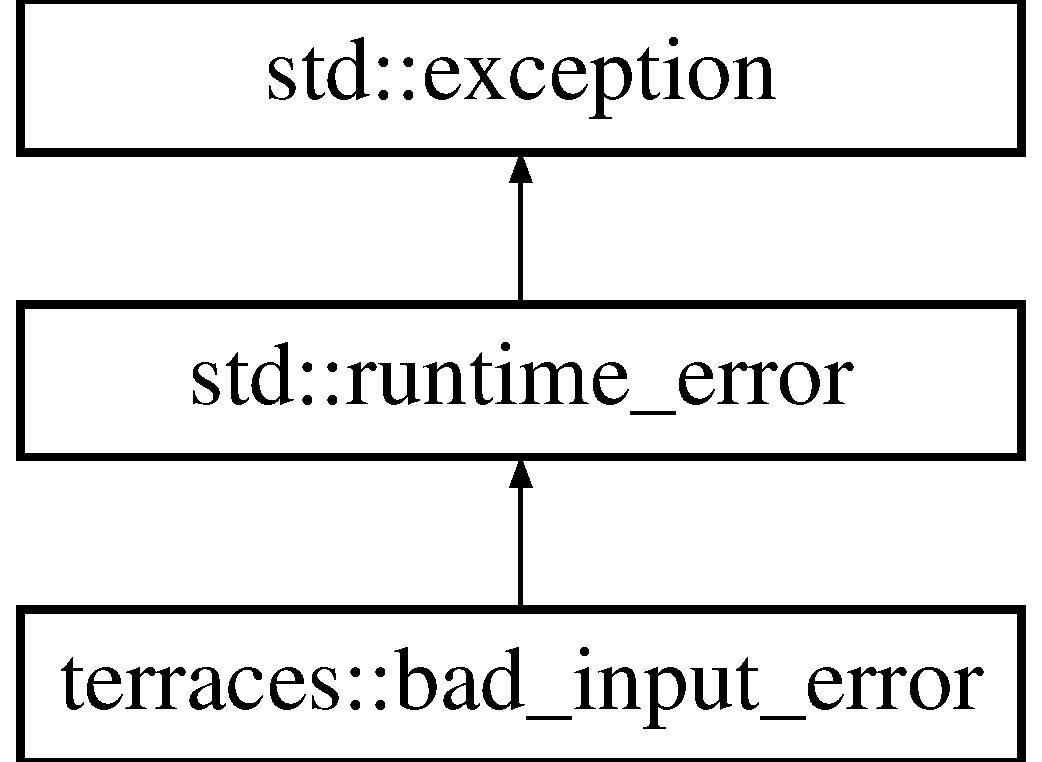
\includegraphics[height=3.000000cm]{classterraces_1_1bad__input__error}
\end{center}
\end{figure}


The documentation for this class was generated from the following file\+:\begin{DoxyCompactItemize}
\item 
include/terraces/\hyperlink{errors_8hpp}{errors.\+hpp}\end{DoxyCompactItemize}

\hypertarget{classterraces_1_1basic__bitvector}{}\section{terraces\+:\+:basic\+\_\+bitvector$<$ Allocator $>$ Class Template Reference}
\label{classterraces_1_1basic__bitvector}\index{terraces\+::basic\+\_\+bitvector$<$ Allocator $>$@{terraces\+::basic\+\_\+bitvector$<$ Allocator $>$}}


{\ttfamily \#include $<$bitvector.\+hpp$>$}

\subsection*{Public Types}
\begin{DoxyCompactItemize}
\item 
using \hyperlink{classterraces_1_1basic__bitvector_ad076eceb68c15a18925cd409e6eaac11}{value\+\_\+type} = \hyperlink{namespaceterraces_adbc33ccb543d1634e96d0eb02e472c77}{index}
\item 
using \hyperlink{classterraces_1_1basic__bitvector_aff8b2ad5a1518f6d8b157df0d2f77bdd}{iterator} = \hyperlink{classterraces_1_1bitvector__iterator}{bitvector\+\_\+iterator}$<$ Allocator $>$
\end{DoxyCompactItemize}
\subsection*{Public Member Functions}
\begin{DoxyCompactItemize}
\item 
\hyperlink{classterraces_1_1basic__bitvector_aeb3cce162b70f7bcbbf51eefad7acce2}{basic\+\_\+bitvector} (\hyperlink{namespaceterraces_adbc33ccb543d1634e96d0eb02e472c77}{index} \hyperlink{classterraces_1_1basic__bitvector_a7a846347ea4c1c1f542ff3331307fdb9}{size}, Allocator alloc)
\item 
void \hyperlink{classterraces_1_1basic__bitvector_a08123518674191423e1f8872ef665650}{set} (\hyperlink{namespaceterraces_adbc33ccb543d1634e96d0eb02e472c77}{index} i)
\item 
void \hyperlink{classterraces_1_1basic__bitvector_a9701e586ebb927deaec8bbff3461c22a}{clr} (\hyperlink{namespaceterraces_adbc33ccb543d1634e96d0eb02e472c77}{index} i)
\item 
void \hyperlink{classterraces_1_1basic__bitvector_ad8f5d3222a2294e462f235ecd9dcb884}{flip} (\hyperlink{namespaceterraces_adbc33ccb543d1634e96d0eb02e472c77}{index} i)
\item 
bool \hyperlink{classterraces_1_1basic__bitvector_a13da8f2c63010742d71c351cababc2d3}{get} (\hyperlink{namespaceterraces_adbc33ccb543d1634e96d0eb02e472c77}{index} i) const
\item 
\hyperlink{namespaceterraces_adbc33ccb543d1634e96d0eb02e472c77}{index} \hyperlink{classterraces_1_1basic__bitvector_a7a846347ea4c1c1f542ff3331307fdb9}{size} () const
\item 
bool \hyperlink{classterraces_1_1basic__bitvector_afe730070283b54ea7013300950488eea}{empty} () const
\item 
void \hyperlink{classterraces_1_1basic__bitvector_aa52688df4fe89e58f1e45b41faf7e068}{blank} ()
\item 
void \hyperlink{classterraces_1_1basic__bitvector_a8a1d7d4cd0916068c73e3412347c7b18}{invert} ()
\item 
void \hyperlink{classterraces_1_1basic__bitvector_ac21b3d7ece4c87cfc4967d7fefb55c54}{bitwise\+\_\+xor} (const \hyperlink{classterraces_1_1basic__bitvector}{basic\+\_\+bitvector}$<$ Allocator $>$ \&other)
\item 
void \hyperlink{classterraces_1_1basic__bitvector_a3e071c2698f1e19765b3c968a80ea65e}{set\+\_\+bitwise\+\_\+or} (const \hyperlink{classterraces_1_1basic__bitvector}{basic\+\_\+bitvector}$<$ Allocator $>$ \&fst, const \hyperlink{classterraces_1_1basic__bitvector}{basic\+\_\+bitvector}$<$ Allocator $>$ \&snd)
\item 
\hyperlink{namespaceterraces_adbc33ccb543d1634e96d0eb02e472c77}{index} \hyperlink{classterraces_1_1basic__bitvector_a43d7e193d6ce2d937039af566f480a74}{first\+\_\+set} () const
\item 
\hyperlink{namespaceterraces_adbc33ccb543d1634e96d0eb02e472c77}{index} \hyperlink{classterraces_1_1basic__bitvector_a21edd3eed32e2c09950d137987457078}{next\+\_\+set} (\hyperlink{namespaceterraces_adbc33ccb543d1634e96d0eb02e472c77}{index} i) const
\item 
\hyperlink{namespaceterraces_adbc33ccb543d1634e96d0eb02e472c77}{index} \hyperlink{classterraces_1_1basic__bitvector_aac46a6f2e72007dc5508f4f3855e236e}{last\+\_\+set} () const
\item 
\hyperlink{classterraces_1_1basic__bitvector_aff8b2ad5a1518f6d8b157df0d2f77bdd}{iterator} \hyperlink{classterraces_1_1basic__bitvector_a205a9008238b8ed80f126230d80a08f3}{begin} () const
\item 
\hyperlink{classterraces_1_1basic__bitvector_aff8b2ad5a1518f6d8b157df0d2f77bdd}{iterator} \hyperlink{classterraces_1_1basic__bitvector_aab7b24b23810e5eda52a99145057d75d}{end} () const
\item 
Allocator \hyperlink{classterraces_1_1basic__bitvector_a50cd443a48618a59a130b0325e75eac4}{get\+\_\+allocator} () const
\item 
bool \hyperlink{classterraces_1_1basic__bitvector_ac09540b4ecb00339e8a9b6a44e1711e3}{operator$<$} (const \hyperlink{classterraces_1_1basic__bitvector}{basic\+\_\+bitvector}$<$ Allocator $>$ \&other) const
\item 
bool \hyperlink{classterraces_1_1basic__bitvector_ad4299081f5f8a3d3d16b662941801400}{operator==} (const \hyperlink{classterraces_1_1basic__bitvector}{basic\+\_\+bitvector}$<$ Allocator $>$ \&other) const
\item 
bool \hyperlink{classterraces_1_1basic__bitvector_a6821bf429f6a9b60065c6e61faadb333}{operator!=} (const \hyperlink{classterraces_1_1basic__bitvector}{basic\+\_\+bitvector}$<$ Allocator $>$ \&other) const
\end{DoxyCompactItemize}
\subsection*{Static Public Member Functions}
\begin{DoxyCompactItemize}
\item 
static \hyperlink{namespaceterraces_adbc33ccb543d1634e96d0eb02e472c77}{index} \hyperlink{classterraces_1_1basic__bitvector_a2256081065bc6537e467f437cfdbef5c}{alloc\+\_\+size} (\hyperlink{namespaceterraces_adbc33ccb543d1634e96d0eb02e472c77}{index} \hyperlink{classterraces_1_1basic__bitvector_a7a846347ea4c1c1f542ff3331307fdb9}{size})
\end{DoxyCompactItemize}
\subsection*{Protected Member Functions}
\begin{DoxyCompactItemize}
\item 
void \hyperlink{classterraces_1_1basic__bitvector_ad5a0a0f50c0f41c8f0f10ea74cd272fa}{add\+\_\+sentinel} ()
\end{DoxyCompactItemize}
\subsection*{Protected Attributes}
\begin{DoxyCompactItemize}
\item 
\hyperlink{namespaceterraces_adbc33ccb543d1634e96d0eb02e472c77}{index} \hyperlink{classterraces_1_1basic__bitvector_ac78f807a89b0bfca92d855ebf1b61206}{m\+\_\+size}
\item 
std\+::vector$<$ \hyperlink{classterraces_1_1basic__bitvector_ad076eceb68c15a18925cd409e6eaac11}{value\+\_\+type}, Allocator $>$ \hyperlink{classterraces_1_1basic__bitvector_a65d3b2d2706a757fa305b725508a3830}{m\+\_\+blocks}
\end{DoxyCompactItemize}


\subsection{Member Typedef Documentation}
\mbox{\Hypertarget{classterraces_1_1basic__bitvector_aff8b2ad5a1518f6d8b157df0d2f77bdd}\label{classterraces_1_1basic__bitvector_aff8b2ad5a1518f6d8b157df0d2f77bdd}} 
\index{terraces\+::basic\+\_\+bitvector@{terraces\+::basic\+\_\+bitvector}!iterator@{iterator}}
\index{iterator@{iterator}!terraces\+::basic\+\_\+bitvector@{terraces\+::basic\+\_\+bitvector}}
\subsubsection{\texorpdfstring{iterator}{iterator}}
{\footnotesize\ttfamily template$<$typename Allocator$>$ \\
using \hyperlink{classterraces_1_1basic__bitvector}{terraces\+::basic\+\_\+bitvector}$<$ Allocator $>$\+::\hyperlink{classterraces_1_1basic__bitvector_aff8b2ad5a1518f6d8b157df0d2f77bdd}{iterator} =  \hyperlink{classterraces_1_1bitvector__iterator}{bitvector\+\_\+iterator}$<$Allocator$>$}

\mbox{\Hypertarget{classterraces_1_1basic__bitvector_ad076eceb68c15a18925cd409e6eaac11}\label{classterraces_1_1basic__bitvector_ad076eceb68c15a18925cd409e6eaac11}} 
\index{terraces\+::basic\+\_\+bitvector@{terraces\+::basic\+\_\+bitvector}!value\+\_\+type@{value\+\_\+type}}
\index{value\+\_\+type@{value\+\_\+type}!terraces\+::basic\+\_\+bitvector@{terraces\+::basic\+\_\+bitvector}}
\subsubsection{\texorpdfstring{value\+\_\+type}{value\_type}}
{\footnotesize\ttfamily template$<$typename Allocator$>$ \\
using \hyperlink{classterraces_1_1basic__bitvector}{terraces\+::basic\+\_\+bitvector}$<$ Allocator $>$\+::\hyperlink{classterraces_1_1basic__bitvector_ad076eceb68c15a18925cd409e6eaac11}{value\+\_\+type} =  \hyperlink{namespaceterraces_adbc33ccb543d1634e96d0eb02e472c77}{index}}



\subsection{Constructor \& Destructor Documentation}
\mbox{\Hypertarget{classterraces_1_1basic__bitvector_aeb3cce162b70f7bcbbf51eefad7acce2}\label{classterraces_1_1basic__bitvector_aeb3cce162b70f7bcbbf51eefad7acce2}} 
\index{terraces\+::basic\+\_\+bitvector@{terraces\+::basic\+\_\+bitvector}!basic\+\_\+bitvector@{basic\+\_\+bitvector}}
\index{basic\+\_\+bitvector@{basic\+\_\+bitvector}!terraces\+::basic\+\_\+bitvector@{terraces\+::basic\+\_\+bitvector}}
\subsubsection{\texorpdfstring{basic\+\_\+bitvector()}{basic\_bitvector()}}
{\footnotesize\ttfamily template$<$typename Allocator$>$ \\
\hyperlink{classterraces_1_1basic__bitvector}{terraces\+::basic\+\_\+bitvector}$<$ Allocator $>$\+::\hyperlink{classterraces_1_1basic__bitvector}{basic\+\_\+bitvector} (\begin{DoxyParamCaption}\item[{\hyperlink{namespaceterraces_adbc33ccb543d1634e96d0eb02e472c77}{index}}]{size,  }\item[{Allocator}]{alloc }\end{DoxyParamCaption})\hspace{0.3cm}{\ttfamily [inline]}}

Initializes a bitvector with given size. 

\subsection{Member Function Documentation}
\mbox{\Hypertarget{classterraces_1_1basic__bitvector_ad5a0a0f50c0f41c8f0f10ea74cd272fa}\label{classterraces_1_1basic__bitvector_ad5a0a0f50c0f41c8f0f10ea74cd272fa}} 
\index{terraces\+::basic\+\_\+bitvector@{terraces\+::basic\+\_\+bitvector}!add\+\_\+sentinel@{add\+\_\+sentinel}}
\index{add\+\_\+sentinel@{add\+\_\+sentinel}!terraces\+::basic\+\_\+bitvector@{terraces\+::basic\+\_\+bitvector}}
\subsubsection{\texorpdfstring{add\+\_\+sentinel()}{add\_sentinel()}}
{\footnotesize\ttfamily template$<$typename Allocator$>$ \\
void \hyperlink{classterraces_1_1basic__bitvector}{terraces\+::basic\+\_\+bitvector}$<$ Allocator $>$\+::add\+\_\+sentinel (\begin{DoxyParamCaption}{ }\end{DoxyParamCaption})\hspace{0.3cm}{\ttfamily [inline]}, {\ttfamily [protected]}}

\mbox{\Hypertarget{classterraces_1_1basic__bitvector_a2256081065bc6537e467f437cfdbef5c}\label{classterraces_1_1basic__bitvector_a2256081065bc6537e467f437cfdbef5c}} 
\index{terraces\+::basic\+\_\+bitvector@{terraces\+::basic\+\_\+bitvector}!alloc\+\_\+size@{alloc\+\_\+size}}
\index{alloc\+\_\+size@{alloc\+\_\+size}!terraces\+::basic\+\_\+bitvector@{terraces\+::basic\+\_\+bitvector}}
\subsubsection{\texorpdfstring{alloc\+\_\+size()}{alloc\_size()}}
{\footnotesize\ttfamily template$<$typename Allocator$>$ \\
static \hyperlink{namespaceterraces_adbc33ccb543d1634e96d0eb02e472c77}{index} \hyperlink{classterraces_1_1basic__bitvector}{terraces\+::basic\+\_\+bitvector}$<$ Allocator $>$\+::alloc\+\_\+size (\begin{DoxyParamCaption}\item[{\hyperlink{namespaceterraces_adbc33ccb543d1634e96d0eb02e472c77}{index}}]{size }\end{DoxyParamCaption})\hspace{0.3cm}{\ttfamily [inline]}, {\ttfamily [static]}}

\mbox{\Hypertarget{classterraces_1_1basic__bitvector_a205a9008238b8ed80f126230d80a08f3}\label{classterraces_1_1basic__bitvector_a205a9008238b8ed80f126230d80a08f3}} 
\index{terraces\+::basic\+\_\+bitvector@{terraces\+::basic\+\_\+bitvector}!begin@{begin}}
\index{begin@{begin}!terraces\+::basic\+\_\+bitvector@{terraces\+::basic\+\_\+bitvector}}
\subsubsection{\texorpdfstring{begin()}{begin()}}
{\footnotesize\ttfamily template$<$typename Alloc $>$ \\
auto \hyperlink{classterraces_1_1basic__bitvector}{terraces\+::basic\+\_\+bitvector}$<$ Alloc $>$\+::begin (\begin{DoxyParamCaption}{ }\end{DoxyParamCaption}) const}

\mbox{\Hypertarget{classterraces_1_1basic__bitvector_ac21b3d7ece4c87cfc4967d7fefb55c54}\label{classterraces_1_1basic__bitvector_ac21b3d7ece4c87cfc4967d7fefb55c54}} 
\index{terraces\+::basic\+\_\+bitvector@{terraces\+::basic\+\_\+bitvector}!bitwise\+\_\+xor@{bitwise\+\_\+xor}}
\index{bitwise\+\_\+xor@{bitwise\+\_\+xor}!terraces\+::basic\+\_\+bitvector@{terraces\+::basic\+\_\+bitvector}}
\subsubsection{\texorpdfstring{bitwise\+\_\+xor()}{bitwise\_xor()}}
{\footnotesize\ttfamily template$<$typename Alloc$>$ \\
void \hyperlink{classterraces_1_1basic__bitvector}{terraces\+::basic\+\_\+bitvector}$<$ Alloc $>$\+::bitwise\+\_\+xor (\begin{DoxyParamCaption}\item[{const \hyperlink{classterraces_1_1basic__bitvector}{basic\+\_\+bitvector}$<$ Alloc $>$ \&}]{other }\end{DoxyParamCaption})}

Applies element-\/wise xor from another bitvector. \mbox{\Hypertarget{classterraces_1_1basic__bitvector_aa52688df4fe89e58f1e45b41faf7e068}\label{classterraces_1_1basic__bitvector_aa52688df4fe89e58f1e45b41faf7e068}} 
\index{terraces\+::basic\+\_\+bitvector@{terraces\+::basic\+\_\+bitvector}!blank@{blank}}
\index{blank@{blank}!terraces\+::basic\+\_\+bitvector@{terraces\+::basic\+\_\+bitvector}}
\subsubsection{\texorpdfstring{blank()}{blank()}}
{\footnotesize\ttfamily template$<$typename Alloc $>$ \\
void \hyperlink{classterraces_1_1basic__bitvector}{terraces\+::basic\+\_\+bitvector}$<$ Alloc $>$\+::blank (\begin{DoxyParamCaption}{ }\end{DoxyParamCaption})}

Clears all bits in the bitvector. \mbox{\Hypertarget{classterraces_1_1basic__bitvector_a9701e586ebb927deaec8bbff3461c22a}\label{classterraces_1_1basic__bitvector_a9701e586ebb927deaec8bbff3461c22a}} 
\index{terraces\+::basic\+\_\+bitvector@{terraces\+::basic\+\_\+bitvector}!clr@{clr}}
\index{clr@{clr}!terraces\+::basic\+\_\+bitvector@{terraces\+::basic\+\_\+bitvector}}
\subsubsection{\texorpdfstring{clr()}{clr()}}
{\footnotesize\ttfamily template$<$typename Allocator$>$ \\
void \hyperlink{classterraces_1_1basic__bitvector}{terraces\+::basic\+\_\+bitvector}$<$ Allocator $>$\+::clr (\begin{DoxyParamCaption}\item[{\hyperlink{namespaceterraces_adbc33ccb543d1634e96d0eb02e472c77}{index}}]{i }\end{DoxyParamCaption})\hspace{0.3cm}{\ttfamily [inline]}}

Clears a bit in the bitvector. \mbox{\Hypertarget{classterraces_1_1basic__bitvector_afe730070283b54ea7013300950488eea}\label{classterraces_1_1basic__bitvector_afe730070283b54ea7013300950488eea}} 
\index{terraces\+::basic\+\_\+bitvector@{terraces\+::basic\+\_\+bitvector}!empty@{empty}}
\index{empty@{empty}!terraces\+::basic\+\_\+bitvector@{terraces\+::basic\+\_\+bitvector}}
\subsubsection{\texorpdfstring{empty()}{empty()}}
{\footnotesize\ttfamily template$<$typename Alloc $>$ \\
bool \hyperlink{classterraces_1_1basic__bitvector}{terraces\+::basic\+\_\+bitvector}$<$ Alloc $>$\+::empty (\begin{DoxyParamCaption}{ }\end{DoxyParamCaption}) const}

Returns true if and only if no bit is set. \mbox{\Hypertarget{classterraces_1_1basic__bitvector_aab7b24b23810e5eda52a99145057d75d}\label{classterraces_1_1basic__bitvector_aab7b24b23810e5eda52a99145057d75d}} 
\index{terraces\+::basic\+\_\+bitvector@{terraces\+::basic\+\_\+bitvector}!end@{end}}
\index{end@{end}!terraces\+::basic\+\_\+bitvector@{terraces\+::basic\+\_\+bitvector}}
\subsubsection{\texorpdfstring{end()}{end()}}
{\footnotesize\ttfamily template$<$typename Alloc $>$ \\
auto \hyperlink{classterraces_1_1basic__bitvector}{terraces\+::basic\+\_\+bitvector}$<$ Alloc $>$\+::end (\begin{DoxyParamCaption}{ }\end{DoxyParamCaption}) const}

\mbox{\Hypertarget{classterraces_1_1basic__bitvector_a43d7e193d6ce2d937039af566f480a74}\label{classterraces_1_1basic__bitvector_a43d7e193d6ce2d937039af566f480a74}} 
\index{terraces\+::basic\+\_\+bitvector@{terraces\+::basic\+\_\+bitvector}!first\+\_\+set@{first\+\_\+set}}
\index{first\+\_\+set@{first\+\_\+set}!terraces\+::basic\+\_\+bitvector@{terraces\+::basic\+\_\+bitvector}}
\subsubsection{\texorpdfstring{first\+\_\+set()}{first\_set()}}
{\footnotesize\ttfamily template$<$typename Alloc $>$ \\
\hyperlink{namespaceterraces_adbc33ccb543d1634e96d0eb02e472c77}{index} \hyperlink{classterraces_1_1basic__bitvector}{terraces\+::basic\+\_\+bitvector}$<$ Alloc $>$\+::first\+\_\+set (\begin{DoxyParamCaption}{ }\end{DoxyParamCaption}) const}

Returns the index of the first set bit or \hyperlink{classterraces_1_1basic__bitvector_a7a846347ea4c1c1f542ff3331307fdb9}{size()} if no bit is set. \mbox{\Hypertarget{classterraces_1_1basic__bitvector_ad8f5d3222a2294e462f235ecd9dcb884}\label{classterraces_1_1basic__bitvector_ad8f5d3222a2294e462f235ecd9dcb884}} 
\index{terraces\+::basic\+\_\+bitvector@{terraces\+::basic\+\_\+bitvector}!flip@{flip}}
\index{flip@{flip}!terraces\+::basic\+\_\+bitvector@{terraces\+::basic\+\_\+bitvector}}
\subsubsection{\texorpdfstring{flip()}{flip()}}
{\footnotesize\ttfamily template$<$typename Allocator$>$ \\
void \hyperlink{classterraces_1_1basic__bitvector}{terraces\+::basic\+\_\+bitvector}$<$ Allocator $>$\+::flip (\begin{DoxyParamCaption}\item[{\hyperlink{namespaceterraces_adbc33ccb543d1634e96d0eb02e472c77}{index}}]{i }\end{DoxyParamCaption})\hspace{0.3cm}{\ttfamily [inline]}}

Flips a bit in the bitvector. \mbox{\Hypertarget{classterraces_1_1basic__bitvector_a13da8f2c63010742d71c351cababc2d3}\label{classterraces_1_1basic__bitvector_a13da8f2c63010742d71c351cababc2d3}} 
\index{terraces\+::basic\+\_\+bitvector@{terraces\+::basic\+\_\+bitvector}!get@{get}}
\index{get@{get}!terraces\+::basic\+\_\+bitvector@{terraces\+::basic\+\_\+bitvector}}
\subsubsection{\texorpdfstring{get()}{get()}}
{\footnotesize\ttfamily template$<$typename Allocator$>$ \\
bool \hyperlink{classterraces_1_1basic__bitvector}{terraces\+::basic\+\_\+bitvector}$<$ Allocator $>$\+::get (\begin{DoxyParamCaption}\item[{\hyperlink{namespaceterraces_adbc33ccb543d1634e96d0eb02e472c77}{index}}]{i }\end{DoxyParamCaption}) const\hspace{0.3cm}{\ttfamily [inline]}}

Returns a bit from the bitvector. \mbox{\Hypertarget{classterraces_1_1basic__bitvector_a50cd443a48618a59a130b0325e75eac4}\label{classterraces_1_1basic__bitvector_a50cd443a48618a59a130b0325e75eac4}} 
\index{terraces\+::basic\+\_\+bitvector@{terraces\+::basic\+\_\+bitvector}!get\+\_\+allocator@{get\+\_\+allocator}}
\index{get\+\_\+allocator@{get\+\_\+allocator}!terraces\+::basic\+\_\+bitvector@{terraces\+::basic\+\_\+bitvector}}
\subsubsection{\texorpdfstring{get\+\_\+allocator()}{get\_allocator()}}
{\footnotesize\ttfamily template$<$typename Allocator$>$ \\
Allocator \hyperlink{classterraces_1_1basic__bitvector}{terraces\+::basic\+\_\+bitvector}$<$ Allocator $>$\+::get\+\_\+allocator (\begin{DoxyParamCaption}{ }\end{DoxyParamCaption}) const\hspace{0.3cm}{\ttfamily [inline]}}

\mbox{\Hypertarget{classterraces_1_1basic__bitvector_a8a1d7d4cd0916068c73e3412347c7b18}\label{classterraces_1_1basic__bitvector_a8a1d7d4cd0916068c73e3412347c7b18}} 
\index{terraces\+::basic\+\_\+bitvector@{terraces\+::basic\+\_\+bitvector}!invert@{invert}}
\index{invert@{invert}!terraces\+::basic\+\_\+bitvector@{terraces\+::basic\+\_\+bitvector}}
\subsubsection{\texorpdfstring{invert()}{invert()}}
{\footnotesize\ttfamily template$<$typename Alloc $>$ \\
void \hyperlink{classterraces_1_1basic__bitvector}{terraces\+::basic\+\_\+bitvector}$<$ Alloc $>$\+::invert (\begin{DoxyParamCaption}{ }\end{DoxyParamCaption})}

Inverts all bits in the bitvector. \mbox{\Hypertarget{classterraces_1_1basic__bitvector_aac46a6f2e72007dc5508f4f3855e236e}\label{classterraces_1_1basic__bitvector_aac46a6f2e72007dc5508f4f3855e236e}} 
\index{terraces\+::basic\+\_\+bitvector@{terraces\+::basic\+\_\+bitvector}!last\+\_\+set@{last\+\_\+set}}
\index{last\+\_\+set@{last\+\_\+set}!terraces\+::basic\+\_\+bitvector@{terraces\+::basic\+\_\+bitvector}}
\subsubsection{\texorpdfstring{last\+\_\+set()}{last\_set()}}
{\footnotesize\ttfamily template$<$typename Allocator$>$ \\
\hyperlink{namespaceterraces_adbc33ccb543d1634e96d0eb02e472c77}{index} \hyperlink{classterraces_1_1basic__bitvector}{terraces\+::basic\+\_\+bitvector}$<$ Allocator $>$\+::last\+\_\+set (\begin{DoxyParamCaption}{ }\end{DoxyParamCaption}) const\hspace{0.3cm}{\ttfamily [inline]}}

Returns the index one past the last element. \mbox{\Hypertarget{classterraces_1_1basic__bitvector_a21edd3eed32e2c09950d137987457078}\label{classterraces_1_1basic__bitvector_a21edd3eed32e2c09950d137987457078}} 
\index{terraces\+::basic\+\_\+bitvector@{terraces\+::basic\+\_\+bitvector}!next\+\_\+set@{next\+\_\+set}}
\index{next\+\_\+set@{next\+\_\+set}!terraces\+::basic\+\_\+bitvector@{terraces\+::basic\+\_\+bitvector}}
\subsubsection{\texorpdfstring{next\+\_\+set()}{next\_set()}}
{\footnotesize\ttfamily template$<$typename Alloc $>$ \\
\hyperlink{namespaceterraces_adbc33ccb543d1634e96d0eb02e472c77}{index} \hyperlink{classterraces_1_1basic__bitvector}{terraces\+::basic\+\_\+bitvector}$<$ Alloc $>$\+::next\+\_\+set (\begin{DoxyParamCaption}\item[{\hyperlink{namespaceterraces_adbc33ccb543d1634e96d0eb02e472c77}{index}}]{i }\end{DoxyParamCaption}) const}

Returns the index of the next set bit after the index or \hyperlink{classterraces_1_1basic__bitvector_a7a846347ea4c1c1f542ff3331307fdb9}{size()} if no bit is set. \mbox{\Hypertarget{classterraces_1_1basic__bitvector_a6821bf429f6a9b60065c6e61faadb333}\label{classterraces_1_1basic__bitvector_a6821bf429f6a9b60065c6e61faadb333}} 
\index{terraces\+::basic\+\_\+bitvector@{terraces\+::basic\+\_\+bitvector}!operator"!=@{operator"!=}}
\index{operator"!=@{operator"!=}!terraces\+::basic\+\_\+bitvector@{terraces\+::basic\+\_\+bitvector}}
\subsubsection{\texorpdfstring{operator"!=()}{operator!=()}}
{\footnotesize\ttfamily template$<$typename Allocator$>$ \\
bool \hyperlink{classterraces_1_1basic__bitvector}{terraces\+::basic\+\_\+bitvector}$<$ Allocator $>$\+::operator!= (\begin{DoxyParamCaption}\item[{const \hyperlink{classterraces_1_1basic__bitvector}{basic\+\_\+bitvector}$<$ Allocator $>$ \&}]{other }\end{DoxyParamCaption}) const\hspace{0.3cm}{\ttfamily [inline]}}

\mbox{\Hypertarget{classterraces_1_1basic__bitvector_ac09540b4ecb00339e8a9b6a44e1711e3}\label{classterraces_1_1basic__bitvector_ac09540b4ecb00339e8a9b6a44e1711e3}} 
\index{terraces\+::basic\+\_\+bitvector@{terraces\+::basic\+\_\+bitvector}!operator$<$@{operator$<$}}
\index{operator$<$@{operator$<$}!terraces\+::basic\+\_\+bitvector@{terraces\+::basic\+\_\+bitvector}}
\subsubsection{\texorpdfstring{operator$<$()}{operator<()}}
{\footnotesize\ttfamily template$<$typename Allocator$>$ \\
bool \hyperlink{classterraces_1_1basic__bitvector}{terraces\+::basic\+\_\+bitvector}$<$ Allocator $>$\+::operator$<$ (\begin{DoxyParamCaption}\item[{const \hyperlink{classterraces_1_1basic__bitvector}{basic\+\_\+bitvector}$<$ Allocator $>$ \&}]{other }\end{DoxyParamCaption}) const\hspace{0.3cm}{\ttfamily [inline]}}

\mbox{\Hypertarget{classterraces_1_1basic__bitvector_ad4299081f5f8a3d3d16b662941801400}\label{classterraces_1_1basic__bitvector_ad4299081f5f8a3d3d16b662941801400}} 
\index{terraces\+::basic\+\_\+bitvector@{terraces\+::basic\+\_\+bitvector}!operator==@{operator==}}
\index{operator==@{operator==}!terraces\+::basic\+\_\+bitvector@{terraces\+::basic\+\_\+bitvector}}
\subsubsection{\texorpdfstring{operator==()}{operator==()}}
{\footnotesize\ttfamily template$<$typename Allocator$>$ \\
bool \hyperlink{classterraces_1_1basic__bitvector}{terraces\+::basic\+\_\+bitvector}$<$ Allocator $>$\+::operator== (\begin{DoxyParamCaption}\item[{const \hyperlink{classterraces_1_1basic__bitvector}{basic\+\_\+bitvector}$<$ Allocator $>$ \&}]{other }\end{DoxyParamCaption}) const\hspace{0.3cm}{\ttfamily [inline]}}

\mbox{\Hypertarget{classterraces_1_1basic__bitvector_a08123518674191423e1f8872ef665650}\label{classterraces_1_1basic__bitvector_a08123518674191423e1f8872ef665650}} 
\index{terraces\+::basic\+\_\+bitvector@{terraces\+::basic\+\_\+bitvector}!set@{set}}
\index{set@{set}!terraces\+::basic\+\_\+bitvector@{terraces\+::basic\+\_\+bitvector}}
\subsubsection{\texorpdfstring{set()}{set()}}
{\footnotesize\ttfamily template$<$typename Allocator$>$ \\
void \hyperlink{classterraces_1_1basic__bitvector}{terraces\+::basic\+\_\+bitvector}$<$ Allocator $>$\+::set (\begin{DoxyParamCaption}\item[{\hyperlink{namespaceterraces_adbc33ccb543d1634e96d0eb02e472c77}{index}}]{i }\end{DoxyParamCaption})\hspace{0.3cm}{\ttfamily [inline]}}

Sets a bit in the bitvector. \mbox{\Hypertarget{classterraces_1_1basic__bitvector_a3e071c2698f1e19765b3c968a80ea65e}\label{classterraces_1_1basic__bitvector_a3e071c2698f1e19765b3c968a80ea65e}} 
\index{terraces\+::basic\+\_\+bitvector@{terraces\+::basic\+\_\+bitvector}!set\+\_\+bitwise\+\_\+or@{set\+\_\+bitwise\+\_\+or}}
\index{set\+\_\+bitwise\+\_\+or@{set\+\_\+bitwise\+\_\+or}!terraces\+::basic\+\_\+bitvector@{terraces\+::basic\+\_\+bitvector}}
\subsubsection{\texorpdfstring{set\+\_\+bitwise\+\_\+or()}{set\_bitwise\_or()}}
{\footnotesize\ttfamily template$<$typename Alloc$>$ \\
void \hyperlink{classterraces_1_1basic__bitvector}{terraces\+::basic\+\_\+bitvector}$<$ Alloc $>$\+::set\+\_\+bitwise\+\_\+or (\begin{DoxyParamCaption}\item[{const \hyperlink{classterraces_1_1basic__bitvector}{basic\+\_\+bitvector}$<$ Alloc $>$ \&}]{fst,  }\item[{const \hyperlink{classterraces_1_1basic__bitvector}{basic\+\_\+bitvector}$<$ Alloc $>$ \&}]{snd }\end{DoxyParamCaption})}

Sets the values of this bitvector to the bitwise or of two bitvectors. \mbox{\Hypertarget{classterraces_1_1basic__bitvector_a7a846347ea4c1c1f542ff3331307fdb9}\label{classterraces_1_1basic__bitvector_a7a846347ea4c1c1f542ff3331307fdb9}} 
\index{terraces\+::basic\+\_\+bitvector@{terraces\+::basic\+\_\+bitvector}!size@{size}}
\index{size@{size}!terraces\+::basic\+\_\+bitvector@{terraces\+::basic\+\_\+bitvector}}
\subsubsection{\texorpdfstring{size()}{size()}}
{\footnotesize\ttfamily template$<$typename Allocator$>$ \\
\hyperlink{namespaceterraces_adbc33ccb543d1634e96d0eb02e472c77}{index} \hyperlink{classterraces_1_1basic__bitvector}{terraces\+::basic\+\_\+bitvector}$<$ Allocator $>$\+::size (\begin{DoxyParamCaption}{ }\end{DoxyParamCaption}) const\hspace{0.3cm}{\ttfamily [inline]}}

Returns the size of the bitvector. 

\subsection{Member Data Documentation}
\mbox{\Hypertarget{classterraces_1_1basic__bitvector_a65d3b2d2706a757fa305b725508a3830}\label{classterraces_1_1basic__bitvector_a65d3b2d2706a757fa305b725508a3830}} 
\index{terraces\+::basic\+\_\+bitvector@{terraces\+::basic\+\_\+bitvector}!m\+\_\+blocks@{m\+\_\+blocks}}
\index{m\+\_\+blocks@{m\+\_\+blocks}!terraces\+::basic\+\_\+bitvector@{terraces\+::basic\+\_\+bitvector}}
\subsubsection{\texorpdfstring{m\+\_\+blocks}{m\_blocks}}
{\footnotesize\ttfamily template$<$typename Allocator$>$ \\
std\+::vector$<$\hyperlink{classterraces_1_1basic__bitvector_ad076eceb68c15a18925cd409e6eaac11}{value\+\_\+type}, Allocator$>$ \hyperlink{classterraces_1_1basic__bitvector}{terraces\+::basic\+\_\+bitvector}$<$ Allocator $>$\+::m\+\_\+blocks\hspace{0.3cm}{\ttfamily [protected]}}

\mbox{\Hypertarget{classterraces_1_1basic__bitvector_ac78f807a89b0bfca92d855ebf1b61206}\label{classterraces_1_1basic__bitvector_ac78f807a89b0bfca92d855ebf1b61206}} 
\index{terraces\+::basic\+\_\+bitvector@{terraces\+::basic\+\_\+bitvector}!m\+\_\+size@{m\+\_\+size}}
\index{m\+\_\+size@{m\+\_\+size}!terraces\+::basic\+\_\+bitvector@{terraces\+::basic\+\_\+bitvector}}
\subsubsection{\texorpdfstring{m\+\_\+size}{m\_size}}
{\footnotesize\ttfamily template$<$typename Allocator$>$ \\
\hyperlink{namespaceterraces_adbc33ccb543d1634e96d0eb02e472c77}{index} \hyperlink{classterraces_1_1basic__bitvector}{terraces\+::basic\+\_\+bitvector}$<$ Allocator $>$\+::m\+\_\+size\hspace{0.3cm}{\ttfamily [protected]}}



The documentation for this class was generated from the following file\+:\begin{DoxyCompactItemize}
\item 
lib/\hyperlink{bitvector_8hpp}{bitvector.\+hpp}\end{DoxyCompactItemize}

\hypertarget{classterraces_1_1basic__ranked__bitvector}{}\section{terraces\+:\+:basic\+\_\+ranked\+\_\+bitvector$<$ Alloc $>$ Class Template Reference}
\label{classterraces_1_1basic__ranked__bitvector}\index{terraces\+::basic\+\_\+ranked\+\_\+bitvector$<$ Alloc $>$@{terraces\+::basic\+\_\+ranked\+\_\+bitvector$<$ Alloc $>$}}


{\ttfamily \#include $<$ranked\+\_\+bitvector.\+hpp$>$}

Inheritance diagram for terraces\+:\+:basic\+\_\+ranked\+\_\+bitvector$<$ Alloc $>$\+:\begin{figure}[H]
\begin{center}
\leavevmode
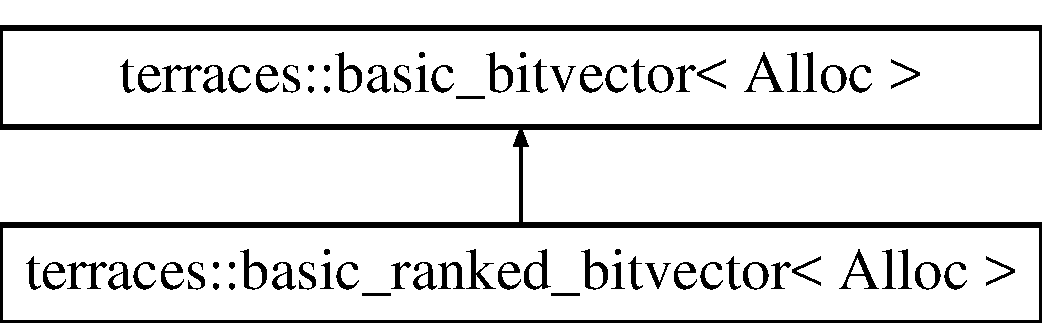
\includegraphics[height=2.000000cm]{classterraces_1_1basic__ranked__bitvector}
\end{center}
\end{figure}
\subsection*{Public Types}
\begin{DoxyCompactItemize}
\item 
using \hyperlink{classterraces_1_1basic__ranked__bitvector_affd5ab8cf4bfba9184dbdd57f4d07bcb}{value\+\_\+type} = typename \hyperlink{classterraces_1_1basic__bitvector}{basic\+\_\+bitvector}$<$ Alloc $>$\+::\hyperlink{classterraces_1_1basic__ranked__bitvector_affd5ab8cf4bfba9184dbdd57f4d07bcb}{value\+\_\+type}
\end{DoxyCompactItemize}
\subsection*{Public Member Functions}
\begin{DoxyCompactItemize}
\item 
\hyperlink{classterraces_1_1basic__ranked__bitvector_a5c6565730dd4f847b9538ea2cb29bdce}{basic\+\_\+ranked\+\_\+bitvector} (\hyperlink{namespaceterraces_adbc33ccb543d1634e96d0eb02e472c77}{index} \hyperlink{classterraces_1_1basic__bitvector_a7a846347ea4c1c1f542ff3331307fdb9}{size}, Alloc alloc)
\item 
\hyperlink{classterraces_1_1basic__ranked__bitvector_ae29465a05501bcc83ce6f03df7d860ae}{m\+\_\+ranks} (base\+::m\+\_\+blocks.\+size(), 0, alloc)
\item 
void \hyperlink{classterraces_1_1basic__ranked__bitvector_ad586efd4696b4d1b9c6a2d01afd7f6e8}{set} (\hyperlink{namespaceterraces_adbc33ccb543d1634e96d0eb02e472c77}{index} i)
\item 
void \hyperlink{classterraces_1_1basic__ranked__bitvector_ab473239260d7a43c5c000f258e69b35f}{clr} (\hyperlink{namespaceterraces_adbc33ccb543d1634e96d0eb02e472c77}{index} i)
\item 
void \hyperlink{classterraces_1_1basic__ranked__bitvector_a4e5caea75842be5a7a598f40e3ae452d}{flip} (\hyperlink{namespaceterraces_adbc33ccb543d1634e96d0eb02e472c77}{index} i)
\item 
void \hyperlink{classterraces_1_1basic__ranked__bitvector_a800cac4946ede86d99fd361e8dabbf02}{blank} ()
\item 
void \hyperlink{classterraces_1_1basic__ranked__bitvector_a1577fa0a6830398e813ea7e6ac3f8587}{invert} ()
\item 
void \hyperlink{classterraces_1_1basic__ranked__bitvector_af574d03b47d01094a2b93569e7dda53e}{bitwise\+\_\+xor} (const \hyperlink{classterraces_1_1basic__bitvector}{basic\+\_\+bitvector}$<$ Alloc $>$ \&other)
\item 
void \hyperlink{classterraces_1_1basic__ranked__bitvector_addd524d9185ed8415909b1bba88102ea}{set\+\_\+bitwise\+\_\+or} (const \hyperlink{classterraces_1_1basic__bitvector}{basic\+\_\+bitvector}$<$ Alloc $>$ \&fst, const \hyperlink{classterraces_1_1basic__bitvector}{basic\+\_\+bitvector}$<$ Alloc $>$ \&snd)
\item 
\hyperlink{namespaceterraces_adbc33ccb543d1634e96d0eb02e472c77}{index} \hyperlink{classterraces_1_1basic__ranked__bitvector_a1d7f3da0a64ed420e4836994cd8cba3c}{count} () const
\item 
void \hyperlink{classterraces_1_1basic__ranked__bitvector_a329e1115f06aa09cf71ec659ba4a0c13}{update\+\_\+ranks} ()
\item 
\hyperlink{namespaceterraces_adbc33ccb543d1634e96d0eb02e472c77}{index} \hyperlink{classterraces_1_1basic__ranked__bitvector_a9e06ab9864653c65a1d4c8c8d72eaac1}{rank} (\hyperlink{namespaceterraces_adbc33ccb543d1634e96d0eb02e472c77}{index} i) const
\item 
\hyperlink{namespaceterraces_adbc33ccb543d1634e96d0eb02e472c77}{index} \hyperlink{classterraces_1_1basic__ranked__bitvector_a56bd3b3ec826c18f78c6bd4012b8da8f}{select} (\hyperlink{namespaceterraces_adbc33ccb543d1634e96d0eb02e472c77}{index} i) const
\end{DoxyCompactItemize}
\subsection*{Additional Inherited Members}


\subsection{Member Typedef Documentation}
\mbox{\Hypertarget{classterraces_1_1basic__ranked__bitvector_affd5ab8cf4bfba9184dbdd57f4d07bcb}\label{classterraces_1_1basic__ranked__bitvector_affd5ab8cf4bfba9184dbdd57f4d07bcb}} 
\index{terraces\+::basic\+\_\+ranked\+\_\+bitvector@{terraces\+::basic\+\_\+ranked\+\_\+bitvector}!value\+\_\+type@{value\+\_\+type}}
\index{value\+\_\+type@{value\+\_\+type}!terraces\+::basic\+\_\+ranked\+\_\+bitvector@{terraces\+::basic\+\_\+ranked\+\_\+bitvector}}
\subsubsection{\texorpdfstring{value\+\_\+type}{value\_type}}
{\footnotesize\ttfamily template$<$typename Alloc$>$ \\
using \hyperlink{classterraces_1_1basic__ranked__bitvector}{terraces\+::basic\+\_\+ranked\+\_\+bitvector}$<$ Alloc $>$\+::\hyperlink{classterraces_1_1basic__ranked__bitvector_affd5ab8cf4bfba9184dbdd57f4d07bcb}{value\+\_\+type} =  typename \hyperlink{classterraces_1_1basic__bitvector}{basic\+\_\+bitvector}$<$Alloc$>$\+::\hyperlink{classterraces_1_1basic__ranked__bitvector_affd5ab8cf4bfba9184dbdd57f4d07bcb}{value\+\_\+type}}



\subsection{Constructor \& Destructor Documentation}
\mbox{\Hypertarget{classterraces_1_1basic__ranked__bitvector_a5c6565730dd4f847b9538ea2cb29bdce}\label{classterraces_1_1basic__ranked__bitvector_a5c6565730dd4f847b9538ea2cb29bdce}} 
\index{terraces\+::basic\+\_\+ranked\+\_\+bitvector@{terraces\+::basic\+\_\+ranked\+\_\+bitvector}!basic\+\_\+ranked\+\_\+bitvector@{basic\+\_\+ranked\+\_\+bitvector}}
\index{basic\+\_\+ranked\+\_\+bitvector@{basic\+\_\+ranked\+\_\+bitvector}!terraces\+::basic\+\_\+ranked\+\_\+bitvector@{terraces\+::basic\+\_\+ranked\+\_\+bitvector}}
\subsubsection{\texorpdfstring{basic\+\_\+ranked\+\_\+bitvector()}{basic\_ranked\_bitvector()}}
{\footnotesize\ttfamily template$<$typename Alloc$>$ \\
\hyperlink{classterraces_1_1basic__ranked__bitvector}{terraces\+::basic\+\_\+ranked\+\_\+bitvector}$<$ Alloc $>$\+::\hyperlink{classterraces_1_1basic__ranked__bitvector}{basic\+\_\+ranked\+\_\+bitvector} (\begin{DoxyParamCaption}\item[{\hyperlink{namespaceterraces_adbc33ccb543d1634e96d0eb02e472c77}{index}}]{size,  }\item[{Alloc}]{alloc }\end{DoxyParamCaption})\hspace{0.3cm}{\ttfamily [inline]}}



\subsection{Member Function Documentation}
\mbox{\Hypertarget{classterraces_1_1basic__ranked__bitvector_af574d03b47d01094a2b93569e7dda53e}\label{classterraces_1_1basic__ranked__bitvector_af574d03b47d01094a2b93569e7dda53e}} 
\index{terraces\+::basic\+\_\+ranked\+\_\+bitvector@{terraces\+::basic\+\_\+ranked\+\_\+bitvector}!bitwise\+\_\+xor@{bitwise\+\_\+xor}}
\index{bitwise\+\_\+xor@{bitwise\+\_\+xor}!terraces\+::basic\+\_\+ranked\+\_\+bitvector@{terraces\+::basic\+\_\+ranked\+\_\+bitvector}}
\subsubsection{\texorpdfstring{bitwise\+\_\+xor()}{bitwise\_xor()}}
{\footnotesize\ttfamily template$<$typename Alloc$>$ \\
void \hyperlink{classterraces_1_1basic__ranked__bitvector}{terraces\+::basic\+\_\+ranked\+\_\+bitvector}$<$ Alloc $>$\+::bitwise\+\_\+xor (\begin{DoxyParamCaption}\item[{const \hyperlink{classterraces_1_1basic__bitvector}{basic\+\_\+bitvector}$<$ Alloc $>$ \&}]{other }\end{DoxyParamCaption})}

Applies element-\/wise xor from another bitvector. \mbox{\Hypertarget{classterraces_1_1basic__ranked__bitvector_a800cac4946ede86d99fd361e8dabbf02}\label{classterraces_1_1basic__ranked__bitvector_a800cac4946ede86d99fd361e8dabbf02}} 
\index{terraces\+::basic\+\_\+ranked\+\_\+bitvector@{terraces\+::basic\+\_\+ranked\+\_\+bitvector}!blank@{blank}}
\index{blank@{blank}!terraces\+::basic\+\_\+ranked\+\_\+bitvector@{terraces\+::basic\+\_\+ranked\+\_\+bitvector}}
\subsubsection{\texorpdfstring{blank()}{blank()}}
{\footnotesize\ttfamily template$<$typename Alloc $>$ \\
void \hyperlink{classterraces_1_1basic__ranked__bitvector}{terraces\+::basic\+\_\+ranked\+\_\+bitvector}$<$ Alloc $>$\+::blank (\begin{DoxyParamCaption}{ }\end{DoxyParamCaption})}

Clears all bits in the bitvector. \mbox{\Hypertarget{classterraces_1_1basic__ranked__bitvector_ab473239260d7a43c5c000f258e69b35f}\label{classterraces_1_1basic__ranked__bitvector_ab473239260d7a43c5c000f258e69b35f}} 
\index{terraces\+::basic\+\_\+ranked\+\_\+bitvector@{terraces\+::basic\+\_\+ranked\+\_\+bitvector}!clr@{clr}}
\index{clr@{clr}!terraces\+::basic\+\_\+ranked\+\_\+bitvector@{terraces\+::basic\+\_\+ranked\+\_\+bitvector}}
\subsubsection{\texorpdfstring{clr()}{clr()}}
{\footnotesize\ttfamily template$<$typename Alloc$>$ \\
void \hyperlink{classterraces_1_1basic__ranked__bitvector}{terraces\+::basic\+\_\+ranked\+\_\+bitvector}$<$ Alloc $>$\+::clr (\begin{DoxyParamCaption}\item[{\hyperlink{namespaceterraces_adbc33ccb543d1634e96d0eb02e472c77}{index}}]{i }\end{DoxyParamCaption})\hspace{0.3cm}{\ttfamily [inline]}}

Clears a bit in the bitvector. \mbox{\Hypertarget{classterraces_1_1basic__ranked__bitvector_a1d7f3da0a64ed420e4836994cd8cba3c}\label{classterraces_1_1basic__ranked__bitvector_a1d7f3da0a64ed420e4836994cd8cba3c}} 
\index{terraces\+::basic\+\_\+ranked\+\_\+bitvector@{terraces\+::basic\+\_\+ranked\+\_\+bitvector}!count@{count}}
\index{count@{count}!terraces\+::basic\+\_\+ranked\+\_\+bitvector@{terraces\+::basic\+\_\+ranked\+\_\+bitvector}}
\subsubsection{\texorpdfstring{count()}{count()}}
{\footnotesize\ttfamily template$<$typename Alloc$>$ \\
\hyperlink{namespaceterraces_adbc33ccb543d1634e96d0eb02e472c77}{index} \hyperlink{classterraces_1_1basic__ranked__bitvector}{terraces\+::basic\+\_\+ranked\+\_\+bitvector}$<$ Alloc $>$\+::count (\begin{DoxyParamCaption}{ }\end{DoxyParamCaption}) const\hspace{0.3cm}{\ttfamily [inline]}}

Returns the number of set bits. \mbox{\Hypertarget{classterraces_1_1basic__ranked__bitvector_a4e5caea75842be5a7a598f40e3ae452d}\label{classterraces_1_1basic__ranked__bitvector_a4e5caea75842be5a7a598f40e3ae452d}} 
\index{terraces\+::basic\+\_\+ranked\+\_\+bitvector@{terraces\+::basic\+\_\+ranked\+\_\+bitvector}!flip@{flip}}
\index{flip@{flip}!terraces\+::basic\+\_\+ranked\+\_\+bitvector@{terraces\+::basic\+\_\+ranked\+\_\+bitvector}}
\subsubsection{\texorpdfstring{flip()}{flip()}}
{\footnotesize\ttfamily template$<$typename Alloc$>$ \\
void \hyperlink{classterraces_1_1basic__ranked__bitvector}{terraces\+::basic\+\_\+ranked\+\_\+bitvector}$<$ Alloc $>$\+::flip (\begin{DoxyParamCaption}\item[{\hyperlink{namespaceterraces_adbc33ccb543d1634e96d0eb02e472c77}{index}}]{i }\end{DoxyParamCaption})\hspace{0.3cm}{\ttfamily [inline]}}

Flips a bit in the bitvector. \mbox{\Hypertarget{classterraces_1_1basic__ranked__bitvector_a1577fa0a6830398e813ea7e6ac3f8587}\label{classterraces_1_1basic__ranked__bitvector_a1577fa0a6830398e813ea7e6ac3f8587}} 
\index{terraces\+::basic\+\_\+ranked\+\_\+bitvector@{terraces\+::basic\+\_\+ranked\+\_\+bitvector}!invert@{invert}}
\index{invert@{invert}!terraces\+::basic\+\_\+ranked\+\_\+bitvector@{terraces\+::basic\+\_\+ranked\+\_\+bitvector}}
\subsubsection{\texorpdfstring{invert()}{invert()}}
{\footnotesize\ttfamily template$<$typename Alloc $>$ \\
void \hyperlink{classterraces_1_1basic__ranked__bitvector}{terraces\+::basic\+\_\+ranked\+\_\+bitvector}$<$ Alloc $>$\+::invert (\begin{DoxyParamCaption}{ }\end{DoxyParamCaption})}

Inverts all bits in the bitvector. \mbox{\Hypertarget{classterraces_1_1basic__ranked__bitvector_ae29465a05501bcc83ce6f03df7d860ae}\label{classterraces_1_1basic__ranked__bitvector_ae29465a05501bcc83ce6f03df7d860ae}} 
\index{terraces\+::basic\+\_\+ranked\+\_\+bitvector@{terraces\+::basic\+\_\+ranked\+\_\+bitvector}!m\+\_\+ranks@{m\+\_\+ranks}}
\index{m\+\_\+ranks@{m\+\_\+ranks}!terraces\+::basic\+\_\+ranked\+\_\+bitvector@{terraces\+::basic\+\_\+ranked\+\_\+bitvector}}
\subsubsection{\texorpdfstring{m\+\_\+ranks()}{m\_ranks()}}
{\footnotesize\ttfamily template$<$typename Alloc$>$ \\
\hyperlink{classterraces_1_1basic__ranked__bitvector}{terraces\+::basic\+\_\+ranked\+\_\+bitvector}$<$ Alloc $>$\+::m\+\_\+ranks (\begin{DoxyParamCaption}\item[{base\+::m\+\_\+blocks.}]{size(),  }\item[{0}]{,  }\item[{alloc}]{ }\end{DoxyParamCaption})\hspace{0.3cm}{\ttfamily [inline]}}

\mbox{\Hypertarget{classterraces_1_1basic__ranked__bitvector_a9e06ab9864653c65a1d4c8c8d72eaac1}\label{classterraces_1_1basic__ranked__bitvector_a9e06ab9864653c65a1d4c8c8d72eaac1}} 
\index{terraces\+::basic\+\_\+ranked\+\_\+bitvector@{terraces\+::basic\+\_\+ranked\+\_\+bitvector}!rank@{rank}}
\index{rank@{rank}!terraces\+::basic\+\_\+ranked\+\_\+bitvector@{terraces\+::basic\+\_\+ranked\+\_\+bitvector}}
\subsubsection{\texorpdfstring{rank()}{rank()}}
{\footnotesize\ttfamily template$<$typename Alloc $>$ \\
\hyperlink{namespaceterraces_adbc33ccb543d1634e96d0eb02e472c77}{index} \hyperlink{classterraces_1_1basic__ranked__bitvector}{terraces\+::basic\+\_\+ranked\+\_\+bitvector}$<$ Alloc $>$\+::rank (\begin{DoxyParamCaption}\item[{\hyperlink{namespaceterraces_adbc33ccb543d1634e96d0eb02e472c77}{index}}]{i }\end{DoxyParamCaption}) const}

Returns the rank of an index, i.\+e. the number of set bits in the range \mbox{[}0..i) \mbox{\Hypertarget{classterraces_1_1basic__ranked__bitvector_a56bd3b3ec826c18f78c6bd4012b8da8f}\label{classterraces_1_1basic__ranked__bitvector_a56bd3b3ec826c18f78c6bd4012b8da8f}} 
\index{terraces\+::basic\+\_\+ranked\+\_\+bitvector@{terraces\+::basic\+\_\+ranked\+\_\+bitvector}!select@{select}}
\index{select@{select}!terraces\+::basic\+\_\+ranked\+\_\+bitvector@{terraces\+::basic\+\_\+ranked\+\_\+bitvector}}
\subsubsection{\texorpdfstring{select()}{select()}}
{\footnotesize\ttfamily template$<$typename Alloc $>$ \\
\hyperlink{namespaceterraces_adbc33ccb543d1634e96d0eb02e472c77}{index} \hyperlink{classterraces_1_1basic__ranked__bitvector}{terraces\+::basic\+\_\+ranked\+\_\+bitvector}$<$ Alloc $>$\+::select (\begin{DoxyParamCaption}\item[{\hyperlink{namespaceterraces_adbc33ccb543d1634e96d0eb02e472c77}{index}}]{i }\end{DoxyParamCaption}) const}

\mbox{\Hypertarget{classterraces_1_1basic__ranked__bitvector_ad586efd4696b4d1b9c6a2d01afd7f6e8}\label{classterraces_1_1basic__ranked__bitvector_ad586efd4696b4d1b9c6a2d01afd7f6e8}} 
\index{terraces\+::basic\+\_\+ranked\+\_\+bitvector@{terraces\+::basic\+\_\+ranked\+\_\+bitvector}!set@{set}}
\index{set@{set}!terraces\+::basic\+\_\+ranked\+\_\+bitvector@{terraces\+::basic\+\_\+ranked\+\_\+bitvector}}
\subsubsection{\texorpdfstring{set()}{set()}}
{\footnotesize\ttfamily template$<$typename Alloc$>$ \\
void \hyperlink{classterraces_1_1basic__ranked__bitvector}{terraces\+::basic\+\_\+ranked\+\_\+bitvector}$<$ Alloc $>$\+::set (\begin{DoxyParamCaption}\item[{\hyperlink{namespaceterraces_adbc33ccb543d1634e96d0eb02e472c77}{index}}]{i }\end{DoxyParamCaption})\hspace{0.3cm}{\ttfamily [inline]}}

Sets a bit in the bitvector. \mbox{\Hypertarget{classterraces_1_1basic__ranked__bitvector_addd524d9185ed8415909b1bba88102ea}\label{classterraces_1_1basic__ranked__bitvector_addd524d9185ed8415909b1bba88102ea}} 
\index{terraces\+::basic\+\_\+ranked\+\_\+bitvector@{terraces\+::basic\+\_\+ranked\+\_\+bitvector}!set\+\_\+bitwise\+\_\+or@{set\+\_\+bitwise\+\_\+or}}
\index{set\+\_\+bitwise\+\_\+or@{set\+\_\+bitwise\+\_\+or}!terraces\+::basic\+\_\+ranked\+\_\+bitvector@{terraces\+::basic\+\_\+ranked\+\_\+bitvector}}
\subsubsection{\texorpdfstring{set\+\_\+bitwise\+\_\+or()}{set\_bitwise\_or()}}
{\footnotesize\ttfamily template$<$typename Alloc$>$ \\
void \hyperlink{classterraces_1_1basic__ranked__bitvector}{terraces\+::basic\+\_\+ranked\+\_\+bitvector}$<$ Alloc $>$\+::set\+\_\+bitwise\+\_\+or (\begin{DoxyParamCaption}\item[{const \hyperlink{classterraces_1_1basic__bitvector}{basic\+\_\+bitvector}$<$ Alloc $>$ \&}]{fst,  }\item[{const \hyperlink{classterraces_1_1basic__bitvector}{basic\+\_\+bitvector}$<$ Alloc $>$ \&}]{snd }\end{DoxyParamCaption})}

Sets the values of this bitvector to the bitwise or of two bitvectors. \mbox{\Hypertarget{classterraces_1_1basic__ranked__bitvector_a329e1115f06aa09cf71ec659ba4a0c13}\label{classterraces_1_1basic__ranked__bitvector_a329e1115f06aa09cf71ec659ba4a0c13}} 
\index{terraces\+::basic\+\_\+ranked\+\_\+bitvector@{terraces\+::basic\+\_\+ranked\+\_\+bitvector}!update\+\_\+ranks@{update\+\_\+ranks}}
\index{update\+\_\+ranks@{update\+\_\+ranks}!terraces\+::basic\+\_\+ranked\+\_\+bitvector@{terraces\+::basic\+\_\+ranked\+\_\+bitvector}}
\subsubsection{\texorpdfstring{update\+\_\+ranks()}{update\_ranks()}}
{\footnotesize\ttfamily template$<$typename Alloc $>$ \\
void \hyperlink{classterraces_1_1basic__ranked__bitvector}{terraces\+::basic\+\_\+ranked\+\_\+bitvector}$<$ Alloc $>$\+::update\+\_\+ranks (\begin{DoxyParamCaption}{ }\end{DoxyParamCaption})}

Updates the internal data structures after editing the vector. 

The documentation for this class was generated from the following file\+:\begin{DoxyCompactItemize}
\item 
lib/\hyperlink{ranked__bitvector_8hpp}{ranked\+\_\+bitvector.\+hpp}\end{DoxyCompactItemize}

\hypertarget{classterraces_1_1bipartition__iterator}{}\section{terraces\+:\+:bipartition\+\_\+iterator Class Reference}
\label{classterraces_1_1bipartition__iterator}\index{terraces\+::bipartition\+\_\+iterator@{terraces\+::bipartition\+\_\+iterator}}


{\ttfamily \#include $<$bipartitions.\+hpp$>$}

\subsection*{Public Member Functions}
\begin{DoxyCompactItemize}
\item 
\hyperlink{classterraces_1_1bipartition__iterator_a5276cb73a4ee31aace8cc8424eda534f}{bipartition\+\_\+iterator} (const \hyperlink{namespaceterraces_acc45ec9c561024c50ecbce5b6738ba08}{ranked\+\_\+bitvector} \&\hyperlink{classterraces_1_1bipartition__iterator_ae3aa95923d3d8004050240f37aea6e65}{leaves}, const \hyperlink{classterraces_1_1union__find}{union\+\_\+find} \&\hyperlink{classterraces_1_1bipartition__iterator_adf63f745fee83552648553ddb0530a3b}{sets}, \hyperlink{classterraces_1_1utils_1_1stack__allocator}{utils\+::stack\+\_\+allocator}$<$ \hyperlink{namespaceterraces_adbc33ccb543d1634e96d0eb02e472c77}{index} $>$)
\item 
void \hyperlink{classterraces_1_1bipartition__iterator_ac072beaef1deb4144217036e5595f4cb}{increase} ()
\item 
bool \hyperlink{classterraces_1_1bipartition__iterator_a6daf5b56669a4df0f1ed2878512c343b}{is\+\_\+valid} () const
\item 
const \hyperlink{namespaceterraces_acc45ec9c561024c50ecbce5b6738ba08}{ranked\+\_\+bitvector} \& \hyperlink{classterraces_1_1bipartition__iterator_abc68c2054681504c6e99e261b47cd22f}{get\+\_\+current\+\_\+set} () const
\item 
void \hyperlink{classterraces_1_1bipartition__iterator_aa8f7242cbf825373196f3fc16b28cfcd}{flip\+\_\+sets} ()
\item 
\hyperlink{namespaceterraces_adbc33ccb543d1634e96d0eb02e472c77}{index} \hyperlink{classterraces_1_1bipartition__iterator_afc11c289f64dd48723ff88e70d67af37}{cur\+\_\+bip} () const
\item 
\hyperlink{namespaceterraces_adbc33ccb543d1634e96d0eb02e472c77}{index} \hyperlink{classterraces_1_1bipartition__iterator_ad73b80dd148b3d236877f812e7ff6fec}{end\+\_\+bip} () const
\item 
\hyperlink{namespaceterraces_adbc33ccb543d1634e96d0eb02e472c77}{index} \hyperlink{classterraces_1_1bipartition__iterator_a6faec2db72f4a8faee4d977a18e97540}{num\+\_\+bip} () const
\item 
const \hyperlink{classterraces_1_1union__find}{union\+\_\+find} \& \hyperlink{classterraces_1_1bipartition__iterator_adf63f745fee83552648553ddb0530a3b}{sets} () const
\item 
const \hyperlink{namespaceterraces_acc45ec9c561024c50ecbce5b6738ba08}{ranked\+\_\+bitvector} \& \hyperlink{classterraces_1_1bipartition__iterator_ae3aa95923d3d8004050240f37aea6e65}{leaves} () const
\end{DoxyCompactItemize}


\subsection{Constructor \& Destructor Documentation}
\mbox{\Hypertarget{classterraces_1_1bipartition__iterator_a5276cb73a4ee31aace8cc8424eda534f}\label{classterraces_1_1bipartition__iterator_a5276cb73a4ee31aace8cc8424eda534f}} 
\index{terraces\+::bipartition\+\_\+iterator@{terraces\+::bipartition\+\_\+iterator}!bipartition\+\_\+iterator@{bipartition\+\_\+iterator}}
\index{bipartition\+\_\+iterator@{bipartition\+\_\+iterator}!terraces\+::bipartition\+\_\+iterator@{terraces\+::bipartition\+\_\+iterator}}
\subsubsection{\texorpdfstring{bipartition\+\_\+iterator()}{bipartition\_iterator()}}
{\footnotesize\ttfamily terraces\+::bipartition\+\_\+iterator\+::bipartition\+\_\+iterator (\begin{DoxyParamCaption}\item[{const \hyperlink{namespaceterraces_acc45ec9c561024c50ecbce5b6738ba08}{ranked\+\_\+bitvector} \&}]{leaves,  }\item[{const \hyperlink{classterraces_1_1union__find}{union\+\_\+find} \&}]{sets,  }\item[{\hyperlink{classterraces_1_1utils_1_1stack__allocator}{utils\+::stack\+\_\+allocator}$<$ \hyperlink{namespaceterraces_adbc33ccb543d1634e96d0eb02e472c77}{index} $>$}]{a }\end{DoxyParamCaption})}



\subsection{Member Function Documentation}
\mbox{\Hypertarget{classterraces_1_1bipartition__iterator_afc11c289f64dd48723ff88e70d67af37}\label{classterraces_1_1bipartition__iterator_afc11c289f64dd48723ff88e70d67af37}} 
\index{terraces\+::bipartition\+\_\+iterator@{terraces\+::bipartition\+\_\+iterator}!cur\+\_\+bip@{cur\+\_\+bip}}
\index{cur\+\_\+bip@{cur\+\_\+bip}!terraces\+::bipartition\+\_\+iterator@{terraces\+::bipartition\+\_\+iterator}}
\subsubsection{\texorpdfstring{cur\+\_\+bip()}{cur\_bip()}}
{\footnotesize\ttfamily \hyperlink{namespaceterraces_adbc33ccb543d1634e96d0eb02e472c77}{index} terraces\+::bipartition\+\_\+iterator\+::cur\+\_\+bip (\begin{DoxyParamCaption}{ }\end{DoxyParamCaption}) const\hspace{0.3cm}{\ttfamily [inline]}}

\mbox{\Hypertarget{classterraces_1_1bipartition__iterator_ad73b80dd148b3d236877f812e7ff6fec}\label{classterraces_1_1bipartition__iterator_ad73b80dd148b3d236877f812e7ff6fec}} 
\index{terraces\+::bipartition\+\_\+iterator@{terraces\+::bipartition\+\_\+iterator}!end\+\_\+bip@{end\+\_\+bip}}
\index{end\+\_\+bip@{end\+\_\+bip}!terraces\+::bipartition\+\_\+iterator@{terraces\+::bipartition\+\_\+iterator}}
\subsubsection{\texorpdfstring{end\+\_\+bip()}{end\_bip()}}
{\footnotesize\ttfamily \hyperlink{namespaceterraces_adbc33ccb543d1634e96d0eb02e472c77}{index} terraces\+::bipartition\+\_\+iterator\+::end\+\_\+bip (\begin{DoxyParamCaption}{ }\end{DoxyParamCaption}) const\hspace{0.3cm}{\ttfamily [inline]}}

\mbox{\Hypertarget{classterraces_1_1bipartition__iterator_aa8f7242cbf825373196f3fc16b28cfcd}\label{classterraces_1_1bipartition__iterator_aa8f7242cbf825373196f3fc16b28cfcd}} 
\index{terraces\+::bipartition\+\_\+iterator@{terraces\+::bipartition\+\_\+iterator}!flip\+\_\+sets@{flip\+\_\+sets}}
\index{flip\+\_\+sets@{flip\+\_\+sets}!terraces\+::bipartition\+\_\+iterator@{terraces\+::bipartition\+\_\+iterator}}
\subsubsection{\texorpdfstring{flip\+\_\+sets()}{flip\_sets()}}
{\footnotesize\ttfamily void terraces\+::bipartition\+\_\+iterator\+::flip\+\_\+sets (\begin{DoxyParamCaption}{ }\end{DoxyParamCaption})}

Switches the current partition with the other partition. \mbox{\Hypertarget{classterraces_1_1bipartition__iterator_abc68c2054681504c6e99e261b47cd22f}\label{classterraces_1_1bipartition__iterator_abc68c2054681504c6e99e261b47cd22f}} 
\index{terraces\+::bipartition\+\_\+iterator@{terraces\+::bipartition\+\_\+iterator}!get\+\_\+current\+\_\+set@{get\+\_\+current\+\_\+set}}
\index{get\+\_\+current\+\_\+set@{get\+\_\+current\+\_\+set}!terraces\+::bipartition\+\_\+iterator@{terraces\+::bipartition\+\_\+iterator}}
\subsubsection{\texorpdfstring{get\+\_\+current\+\_\+set()}{get\_current\_set()}}
{\footnotesize\ttfamily const \hyperlink{namespaceterraces_acc45ec9c561024c50ecbce5b6738ba08}{ranked\+\_\+bitvector} \& terraces\+::bipartition\+\_\+iterator\+::get\+\_\+current\+\_\+set (\begin{DoxyParamCaption}{ }\end{DoxyParamCaption}) const}

Returns the current partition. Switching to the other partition can be done via flip(). \mbox{\Hypertarget{classterraces_1_1bipartition__iterator_ac072beaef1deb4144217036e5595f4cb}\label{classterraces_1_1bipartition__iterator_ac072beaef1deb4144217036e5595f4cb}} 
\index{terraces\+::bipartition\+\_\+iterator@{terraces\+::bipartition\+\_\+iterator}!increase@{increase}}
\index{increase@{increase}!terraces\+::bipartition\+\_\+iterator@{terraces\+::bipartition\+\_\+iterator}}
\subsubsection{\texorpdfstring{increase()}{increase()}}
{\footnotesize\ttfamily void terraces\+::bipartition\+\_\+iterator\+::increase (\begin{DoxyParamCaption}{ }\end{DoxyParamCaption})}

Moves to the next bipartition. \mbox{\Hypertarget{classterraces_1_1bipartition__iterator_a6daf5b56669a4df0f1ed2878512c343b}\label{classterraces_1_1bipartition__iterator_a6daf5b56669a4df0f1ed2878512c343b}} 
\index{terraces\+::bipartition\+\_\+iterator@{terraces\+::bipartition\+\_\+iterator}!is\+\_\+valid@{is\+\_\+valid}}
\index{is\+\_\+valid@{is\+\_\+valid}!terraces\+::bipartition\+\_\+iterator@{terraces\+::bipartition\+\_\+iterator}}
\subsubsection{\texorpdfstring{is\+\_\+valid()}{is\_valid()}}
{\footnotesize\ttfamily bool terraces\+::bipartition\+\_\+iterator\+::is\+\_\+valid (\begin{DoxyParamCaption}{ }\end{DoxyParamCaption}) const}

Returns true if this bipartition is valid. \mbox{\Hypertarget{classterraces_1_1bipartition__iterator_ae3aa95923d3d8004050240f37aea6e65}\label{classterraces_1_1bipartition__iterator_ae3aa95923d3d8004050240f37aea6e65}} 
\index{terraces\+::bipartition\+\_\+iterator@{terraces\+::bipartition\+\_\+iterator}!leaves@{leaves}}
\index{leaves@{leaves}!terraces\+::bipartition\+\_\+iterator@{terraces\+::bipartition\+\_\+iterator}}
\subsubsection{\texorpdfstring{leaves()}{leaves()}}
{\footnotesize\ttfamily const \hyperlink{namespaceterraces_acc45ec9c561024c50ecbce5b6738ba08}{ranked\+\_\+bitvector}\& terraces\+::bipartition\+\_\+iterator\+::leaves (\begin{DoxyParamCaption}{ }\end{DoxyParamCaption}) const\hspace{0.3cm}{\ttfamily [inline]}}

\mbox{\Hypertarget{classterraces_1_1bipartition__iterator_a6faec2db72f4a8faee4d977a18e97540}\label{classterraces_1_1bipartition__iterator_a6faec2db72f4a8faee4d977a18e97540}} 
\index{terraces\+::bipartition\+\_\+iterator@{terraces\+::bipartition\+\_\+iterator}!num\+\_\+bip@{num\+\_\+bip}}
\index{num\+\_\+bip@{num\+\_\+bip}!terraces\+::bipartition\+\_\+iterator@{terraces\+::bipartition\+\_\+iterator}}
\subsubsection{\texorpdfstring{num\+\_\+bip()}{num\_bip()}}
{\footnotesize\ttfamily \hyperlink{namespaceterraces_adbc33ccb543d1634e96d0eb02e472c77}{index} terraces\+::bipartition\+\_\+iterator\+::num\+\_\+bip (\begin{DoxyParamCaption}{ }\end{DoxyParamCaption}) const\hspace{0.3cm}{\ttfamily [inline]}}

\mbox{\Hypertarget{classterraces_1_1bipartition__iterator_adf63f745fee83552648553ddb0530a3b}\label{classterraces_1_1bipartition__iterator_adf63f745fee83552648553ddb0530a3b}} 
\index{terraces\+::bipartition\+\_\+iterator@{terraces\+::bipartition\+\_\+iterator}!sets@{sets}}
\index{sets@{sets}!terraces\+::bipartition\+\_\+iterator@{terraces\+::bipartition\+\_\+iterator}}
\subsubsection{\texorpdfstring{sets()}{sets()}}
{\footnotesize\ttfamily const \hyperlink{classterraces_1_1union__find}{union\+\_\+find}\& terraces\+::bipartition\+\_\+iterator\+::sets (\begin{DoxyParamCaption}{ }\end{DoxyParamCaption}) const\hspace{0.3cm}{\ttfamily [inline]}}



The documentation for this class was generated from the following files\+:\begin{DoxyCompactItemize}
\item 
lib/\hyperlink{bipartitions_8hpp}{bipartitions.\+hpp}\item 
lib/\hyperlink{lib_2bipartitions_8cpp}{bipartitions.\+cpp}\end{DoxyCompactItemize}

\hypertarget{classterraces_1_1bitmatrix}{}\section{terraces\+:\+:bitmatrix Class Reference}
\label{classterraces_1_1bitmatrix}\index{terraces\+::bitmatrix@{terraces\+::bitmatrix}}


{\ttfamily \#include $<$bitmatrix.\+hpp$>$}

\subsection*{Public Member Functions}
\begin{DoxyCompactItemize}
\item 
\hyperlink{classterraces_1_1bitmatrix_ab3210e10f4ffb9850325e93db17b9e0d}{bitmatrix} (\hyperlink{namespaceterraces_adbc33ccb543d1634e96d0eb02e472c77}{index} \hyperlink{classterraces_1_1bitmatrix_a7e19b0df5f60d1bd76cda27987bac1ad}{rows}, \hyperlink{namespaceterraces_adbc33ccb543d1634e96d0eb02e472c77}{index} \hyperlink{classterraces_1_1bitmatrix_a55c1ef8f0554b8b82c2f4f86e8d4a0ef}{cols})
\item 
\hyperlink{namespaceterraces_adbc33ccb543d1634e96d0eb02e472c77}{index} \hyperlink{classterraces_1_1bitmatrix_a7e19b0df5f60d1bd76cda27987bac1ad}{rows} () const
\item 
\hyperlink{namespaceterraces_adbc33ccb543d1634e96d0eb02e472c77}{index} \hyperlink{classterraces_1_1bitmatrix_a55c1ef8f0554b8b82c2f4f86e8d4a0ef}{cols} () const
\item 
bool \hyperlink{classterraces_1_1bitmatrix_aef01e1c2bc601f43786343adf8b3876e}{get} (\hyperlink{namespaceterraces_adbc33ccb543d1634e96d0eb02e472c77}{index} row, \hyperlink{namespaceterraces_adbc33ccb543d1634e96d0eb02e472c77}{index} col) const
\item 
void \hyperlink{classterraces_1_1bitmatrix_abced1ac3b008ea34b2917e5a4b82a7d4}{set} (\hyperlink{namespaceterraces_adbc33ccb543d1634e96d0eb02e472c77}{index} row, \hyperlink{namespaceterraces_adbc33ccb543d1634e96d0eb02e472c77}{index} col, bool val)
\item 
void \hyperlink{classterraces_1_1bitmatrix_a36a4964456f0d7f0eeb389e42124fa84}{row\+\_\+or} (\hyperlink{namespaceterraces_adbc33ccb543d1634e96d0eb02e472c77}{index} in1, \hyperlink{namespaceterraces_adbc33ccb543d1634e96d0eb02e472c77}{index} in2, \hyperlink{namespaceterraces_adbc33ccb543d1634e96d0eb02e472c77}{index} out)
\item 
\hyperlink{classterraces_1_1bitmatrix}{bitmatrix} \hyperlink{classterraces_1_1bitmatrix_a0da6fd3a2321c19fdb802ba825d83d24}{get\+\_\+cols} (const std\+::vector$<$ std\+::size\+\_\+t $>$ \&\hyperlink{classterraces_1_1bitmatrix_a55c1ef8f0554b8b82c2f4f86e8d4a0ef}{cols}) const
\end{DoxyCompactItemize}


\subsection{Constructor \& Destructor Documentation}
\mbox{\Hypertarget{classterraces_1_1bitmatrix_ab3210e10f4ffb9850325e93db17b9e0d}\label{classterraces_1_1bitmatrix_ab3210e10f4ffb9850325e93db17b9e0d}} 
\index{terraces\+::bitmatrix@{terraces\+::bitmatrix}!bitmatrix@{bitmatrix}}
\index{bitmatrix@{bitmatrix}!terraces\+::bitmatrix@{terraces\+::bitmatrix}}
\subsubsection{\texorpdfstring{bitmatrix()}{bitmatrix()}}
{\footnotesize\ttfamily terraces\+::bitmatrix\+::bitmatrix (\begin{DoxyParamCaption}\item[{\hyperlink{namespaceterraces_adbc33ccb543d1634e96d0eb02e472c77}{index}}]{rows,  }\item[{\hyperlink{namespaceterraces_adbc33ccb543d1634e96d0eb02e472c77}{index}}]{cols }\end{DoxyParamCaption})}



\subsection{Member Function Documentation}
\mbox{\Hypertarget{classterraces_1_1bitmatrix_a55c1ef8f0554b8b82c2f4f86e8d4a0ef}\label{classterraces_1_1bitmatrix_a55c1ef8f0554b8b82c2f4f86e8d4a0ef}} 
\index{terraces\+::bitmatrix@{terraces\+::bitmatrix}!cols@{cols}}
\index{cols@{cols}!terraces\+::bitmatrix@{terraces\+::bitmatrix}}
\subsubsection{\texorpdfstring{cols()}{cols()}}
{\footnotesize\ttfamily \hyperlink{namespaceterraces_adbc33ccb543d1634e96d0eb02e472c77}{index} terraces\+::bitmatrix\+::cols (\begin{DoxyParamCaption}{ }\end{DoxyParamCaption}) const}

\mbox{\Hypertarget{classterraces_1_1bitmatrix_aef01e1c2bc601f43786343adf8b3876e}\label{classterraces_1_1bitmatrix_aef01e1c2bc601f43786343adf8b3876e}} 
\index{terraces\+::bitmatrix@{terraces\+::bitmatrix}!get@{get}}
\index{get@{get}!terraces\+::bitmatrix@{terraces\+::bitmatrix}}
\subsubsection{\texorpdfstring{get()}{get()}}
{\footnotesize\ttfamily bool terraces\+::bitmatrix\+::get (\begin{DoxyParamCaption}\item[{\hyperlink{namespaceterraces_adbc33ccb543d1634e96d0eb02e472c77}{index}}]{row,  }\item[{\hyperlink{namespaceterraces_adbc33ccb543d1634e96d0eb02e472c77}{index}}]{col }\end{DoxyParamCaption}) const}

\mbox{\Hypertarget{classterraces_1_1bitmatrix_a0da6fd3a2321c19fdb802ba825d83d24}\label{classterraces_1_1bitmatrix_a0da6fd3a2321c19fdb802ba825d83d24}} 
\index{terraces\+::bitmatrix@{terraces\+::bitmatrix}!get\+\_\+cols@{get\+\_\+cols}}
\index{get\+\_\+cols@{get\+\_\+cols}!terraces\+::bitmatrix@{terraces\+::bitmatrix}}
\subsubsection{\texorpdfstring{get\+\_\+cols()}{get\_cols()}}
{\footnotesize\ttfamily \hyperlink{classterraces_1_1bitmatrix}{bitmatrix} terraces\+::bitmatrix\+::get\+\_\+cols (\begin{DoxyParamCaption}\item[{const std\+::vector$<$ std\+::size\+\_\+t $>$ \&}]{cols }\end{DoxyParamCaption}) const}

\mbox{\Hypertarget{classterraces_1_1bitmatrix_a36a4964456f0d7f0eeb389e42124fa84}\label{classterraces_1_1bitmatrix_a36a4964456f0d7f0eeb389e42124fa84}} 
\index{terraces\+::bitmatrix@{terraces\+::bitmatrix}!row\+\_\+or@{row\+\_\+or}}
\index{row\+\_\+or@{row\+\_\+or}!terraces\+::bitmatrix@{terraces\+::bitmatrix}}
\subsubsection{\texorpdfstring{row\+\_\+or()}{row\_or()}}
{\footnotesize\ttfamily void terraces\+::bitmatrix\+::row\+\_\+or (\begin{DoxyParamCaption}\item[{\hyperlink{namespaceterraces_adbc33ccb543d1634e96d0eb02e472c77}{index}}]{in1,  }\item[{\hyperlink{namespaceterraces_adbc33ccb543d1634e96d0eb02e472c77}{index}}]{in2,  }\item[{\hyperlink{namespaceterraces_adbc33ccb543d1634e96d0eb02e472c77}{index}}]{out }\end{DoxyParamCaption})}

Writes the bit rows \textquotesingle{}in1\textquotesingle{} and \textquotesingle{}in2\textquotesingle{} to row \textquotesingle{}out\textquotesingle{}. \mbox{\Hypertarget{classterraces_1_1bitmatrix_a7e19b0df5f60d1bd76cda27987bac1ad}\label{classterraces_1_1bitmatrix_a7e19b0df5f60d1bd76cda27987bac1ad}} 
\index{terraces\+::bitmatrix@{terraces\+::bitmatrix}!rows@{rows}}
\index{rows@{rows}!terraces\+::bitmatrix@{terraces\+::bitmatrix}}
\subsubsection{\texorpdfstring{rows()}{rows()}}
{\footnotesize\ttfamily \hyperlink{namespaceterraces_adbc33ccb543d1634e96d0eb02e472c77}{index} terraces\+::bitmatrix\+::rows (\begin{DoxyParamCaption}{ }\end{DoxyParamCaption}) const}

\mbox{\Hypertarget{classterraces_1_1bitmatrix_abced1ac3b008ea34b2917e5a4b82a7d4}\label{classterraces_1_1bitmatrix_abced1ac3b008ea34b2917e5a4b82a7d4}} 
\index{terraces\+::bitmatrix@{terraces\+::bitmatrix}!set@{set}}
\index{set@{set}!terraces\+::bitmatrix@{terraces\+::bitmatrix}}
\subsubsection{\texorpdfstring{set()}{set()}}
{\footnotesize\ttfamily void terraces\+::bitmatrix\+::set (\begin{DoxyParamCaption}\item[{\hyperlink{namespaceterraces_adbc33ccb543d1634e96d0eb02e472c77}{index}}]{row,  }\item[{\hyperlink{namespaceterraces_adbc33ccb543d1634e96d0eb02e472c77}{index}}]{col,  }\item[{bool}]{val }\end{DoxyParamCaption})}



The documentation for this class was generated from the following files\+:\begin{DoxyCompactItemize}
\item 
include/terraces/\hyperlink{bitmatrix_8hpp}{bitmatrix.\+hpp}\item 
lib/\hyperlink{lib_2bitmatrix_8cpp}{bitmatrix.\+cpp}\end{DoxyCompactItemize}

\hypertarget{classterraces_1_1bitvector__iterator}{}\section{terraces\+:\+:bitvector\+\_\+iterator$<$ Alloc $>$ Class Template Reference}
\label{classterraces_1_1bitvector__iterator}\index{terraces\+::bitvector\+\_\+iterator$<$ Alloc $>$@{terraces\+::bitvector\+\_\+iterator$<$ Alloc $>$}}


{\ttfamily \#include $<$bitvector.\+hpp$>$}

\subsection*{Public Types}
\begin{DoxyCompactItemize}
\item 
using \hyperlink{classterraces_1_1bitvector__iterator_a8156fa80ed2f7604e66ed92516064472}{value\+\_\+type} = typename Alloc\+::value\+\_\+type
\end{DoxyCompactItemize}
\subsection*{Public Member Functions}
\begin{DoxyCompactItemize}
\item 
\hyperlink{classterraces_1_1bitvector__iterator_afebccf304754e00d27e87508c4e43a4c}{bitvector\+\_\+iterator} (const \hyperlink{classterraces_1_1basic__bitvector}{basic\+\_\+bitvector}$<$ Alloc $>$ \&set, \hyperlink{namespaceterraces_adbc33ccb543d1634e96d0eb02e472c77}{index} i)
\item 
\hyperlink{classterraces_1_1bitvector__iterator}{bitvector\+\_\+iterator} \& \hyperlink{classterraces_1_1bitvector__iterator_ae20702cafbc74443374d264031481b30}{operator++} ()
\item 
bool \hyperlink{classterraces_1_1bitvector__iterator_a33e2ed2d92f8b24558f758ba340d384d}{operator==} (const \hyperlink{classterraces_1_1bitvector__iterator}{bitvector\+\_\+iterator} \&other) const
\item 
bool \hyperlink{classterraces_1_1bitvector__iterator_aacb89a9a24c74fcaadefff23a5016ce0}{operator!=} (const \hyperlink{classterraces_1_1bitvector__iterator}{bitvector\+\_\+iterator} \&other) const
\item 
const \hyperlink{namespaceterraces_adbc33ccb543d1634e96d0eb02e472c77}{index} \& \hyperlink{classterraces_1_1bitvector__iterator_ae71cae069ce0644f658f71763b65c49d}{operator$\ast$} () const
\end{DoxyCompactItemize}


\subsection{Member Typedef Documentation}
\mbox{\Hypertarget{classterraces_1_1bitvector__iterator_a8156fa80ed2f7604e66ed92516064472}\label{classterraces_1_1bitvector__iterator_a8156fa80ed2f7604e66ed92516064472}} 
\index{terraces\+::bitvector\+\_\+iterator@{terraces\+::bitvector\+\_\+iterator}!value\+\_\+type@{value\+\_\+type}}
\index{value\+\_\+type@{value\+\_\+type}!terraces\+::bitvector\+\_\+iterator@{terraces\+::bitvector\+\_\+iterator}}
\subsubsection{\texorpdfstring{value\+\_\+type}{value\_type}}
{\footnotesize\ttfamily template$<$typename Alloc $>$ \\
using \hyperlink{classterraces_1_1bitvector__iterator}{terraces\+::bitvector\+\_\+iterator}$<$ Alloc $>$\+::\hyperlink{classterraces_1_1bitvector__iterator_a8156fa80ed2f7604e66ed92516064472}{value\+\_\+type} =  typename Alloc\+::value\+\_\+type}



\subsection{Constructor \& Destructor Documentation}
\mbox{\Hypertarget{classterraces_1_1bitvector__iterator_afebccf304754e00d27e87508c4e43a4c}\label{classterraces_1_1bitvector__iterator_afebccf304754e00d27e87508c4e43a4c}} 
\index{terraces\+::bitvector\+\_\+iterator@{terraces\+::bitvector\+\_\+iterator}!bitvector\+\_\+iterator@{bitvector\+\_\+iterator}}
\index{bitvector\+\_\+iterator@{bitvector\+\_\+iterator}!terraces\+::bitvector\+\_\+iterator@{terraces\+::bitvector\+\_\+iterator}}
\subsubsection{\texorpdfstring{bitvector\+\_\+iterator()}{bitvector\_iterator()}}
{\footnotesize\ttfamily template$<$typename Alloc $>$ \\
\hyperlink{classterraces_1_1bitvector__iterator}{terraces\+::bitvector\+\_\+iterator}$<$ Alloc $>$\+::\hyperlink{classterraces_1_1bitvector__iterator}{bitvector\+\_\+iterator} (\begin{DoxyParamCaption}\item[{const \hyperlink{classterraces_1_1basic__bitvector}{basic\+\_\+bitvector}$<$ Alloc $>$ \&}]{set,  }\item[{\hyperlink{namespaceterraces_adbc33ccb543d1634e96d0eb02e472c77}{index}}]{i }\end{DoxyParamCaption})\hspace{0.3cm}{\ttfamily [inline]}}



\subsection{Member Function Documentation}
\mbox{\Hypertarget{classterraces_1_1bitvector__iterator_aacb89a9a24c74fcaadefff23a5016ce0}\label{classterraces_1_1bitvector__iterator_aacb89a9a24c74fcaadefff23a5016ce0}} 
\index{terraces\+::bitvector\+\_\+iterator@{terraces\+::bitvector\+\_\+iterator}!operator"!=@{operator"!=}}
\index{operator"!=@{operator"!=}!terraces\+::bitvector\+\_\+iterator@{terraces\+::bitvector\+\_\+iterator}}
\subsubsection{\texorpdfstring{operator"!=()}{operator!=()}}
{\footnotesize\ttfamily template$<$typename Alloc $>$ \\
bool \hyperlink{classterraces_1_1bitvector__iterator}{terraces\+::bitvector\+\_\+iterator}$<$ Alloc $>$\+::operator!= (\begin{DoxyParamCaption}\item[{const \hyperlink{classterraces_1_1bitvector__iterator}{bitvector\+\_\+iterator}$<$ Alloc $>$ \&}]{other }\end{DoxyParamCaption}) const\hspace{0.3cm}{\ttfamily [inline]}}

\mbox{\Hypertarget{classterraces_1_1bitvector__iterator_ae71cae069ce0644f658f71763b65c49d}\label{classterraces_1_1bitvector__iterator_ae71cae069ce0644f658f71763b65c49d}} 
\index{terraces\+::bitvector\+\_\+iterator@{terraces\+::bitvector\+\_\+iterator}!operator$\ast$@{operator$\ast$}}
\index{operator$\ast$@{operator$\ast$}!terraces\+::bitvector\+\_\+iterator@{terraces\+::bitvector\+\_\+iterator}}
\subsubsection{\texorpdfstring{operator$\ast$()}{operator*()}}
{\footnotesize\ttfamily template$<$typename Alloc $>$ \\
const \hyperlink{namespaceterraces_adbc33ccb543d1634e96d0eb02e472c77}{index}\& \hyperlink{classterraces_1_1bitvector__iterator}{terraces\+::bitvector\+\_\+iterator}$<$ Alloc $>$\+::operator$\ast$ (\begin{DoxyParamCaption}{ }\end{DoxyParamCaption}) const\hspace{0.3cm}{\ttfamily [inline]}}

\mbox{\Hypertarget{classterraces_1_1bitvector__iterator_ae20702cafbc74443374d264031481b30}\label{classterraces_1_1bitvector__iterator_ae20702cafbc74443374d264031481b30}} 
\index{terraces\+::bitvector\+\_\+iterator@{terraces\+::bitvector\+\_\+iterator}!operator++@{operator++}}
\index{operator++@{operator++}!terraces\+::bitvector\+\_\+iterator@{terraces\+::bitvector\+\_\+iterator}}
\subsubsection{\texorpdfstring{operator++()}{operator++()}}
{\footnotesize\ttfamily template$<$typename Alloc $>$ \\
\hyperlink{classterraces_1_1bitvector__iterator}{bitvector\+\_\+iterator}\& \hyperlink{classterraces_1_1bitvector__iterator}{terraces\+::bitvector\+\_\+iterator}$<$ Alloc $>$\+::operator++ (\begin{DoxyParamCaption}{ }\end{DoxyParamCaption})\hspace{0.3cm}{\ttfamily [inline]}}

\mbox{\Hypertarget{classterraces_1_1bitvector__iterator_a33e2ed2d92f8b24558f758ba340d384d}\label{classterraces_1_1bitvector__iterator_a33e2ed2d92f8b24558f758ba340d384d}} 
\index{terraces\+::bitvector\+\_\+iterator@{terraces\+::bitvector\+\_\+iterator}!operator==@{operator==}}
\index{operator==@{operator==}!terraces\+::bitvector\+\_\+iterator@{terraces\+::bitvector\+\_\+iterator}}
\subsubsection{\texorpdfstring{operator==()}{operator==()}}
{\footnotesize\ttfamily template$<$typename Alloc $>$ \\
bool \hyperlink{classterraces_1_1bitvector__iterator}{terraces\+::bitvector\+\_\+iterator}$<$ Alloc $>$\+::operator== (\begin{DoxyParamCaption}\item[{const \hyperlink{classterraces_1_1bitvector__iterator}{bitvector\+\_\+iterator}$<$ Alloc $>$ \&}]{other }\end{DoxyParamCaption}) const\hspace{0.3cm}{\ttfamily [inline]}}



The documentation for this class was generated from the following file\+:\begin{DoxyCompactItemize}
\item 
lib/\hyperlink{bitvector_8hpp}{bitvector.\+hpp}\end{DoxyCompactItemize}

\hypertarget{classterraces_1_1variants_1_1check__callback}{}\section{terraces\+:\+:variants\+:\+:check\+\_\+callback Class Reference}
\label{classterraces_1_1variants_1_1check__callback}\index{terraces\+::variants\+::check\+\_\+callback@{terraces\+::variants\+::check\+\_\+callback}}


{\ttfamily \#include $<$supertree\+\_\+variants.\+hpp$>$}

Inheritance diagram for terraces\+:\+:variants\+:\+:check\+\_\+callback\+:\begin{figure}[H]
\begin{center}
\leavevmode
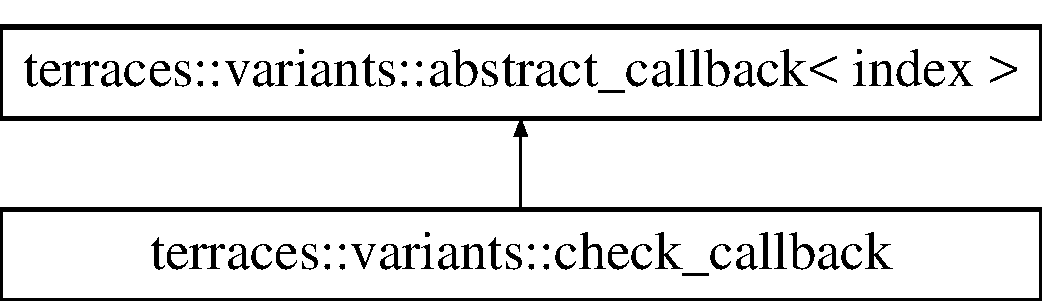
\includegraphics[height=2.000000cm]{classterraces_1_1variants_1_1check__callback}
\end{center}
\end{figure}
\subsection*{Public Types}
\begin{DoxyCompactItemize}
\item 
using \hyperlink{classterraces_1_1variants_1_1check__callback_ab5d02c5889d54c20a3e74d104aab9893}{return\+\_\+type} = \hyperlink{namespaceterraces_adbc33ccb543d1634e96d0eb02e472c77}{index}
\end{DoxyCompactItemize}
\subsection*{Public Member Functions}
\begin{DoxyCompactItemize}
\item 
\hyperlink{namespaceterraces_adbc33ccb543d1634e96d0eb02e472c77}{index} \hyperlink{classterraces_1_1variants_1_1check__callback_aa681c54dfde633ae4707d7e5bd5f19a0}{base\+\_\+one\+\_\+leaf} (\hyperlink{namespaceterraces_adbc33ccb543d1634e96d0eb02e472c77}{index})
\item 
\hyperlink{namespaceterraces_adbc33ccb543d1634e96d0eb02e472c77}{index} \hyperlink{classterraces_1_1variants_1_1check__callback_a103b75a312ea500b98981324eae79635}{base\+\_\+two\+\_\+leaves} (\hyperlink{namespaceterraces_adbc33ccb543d1634e96d0eb02e472c77}{index}, \hyperlink{namespaceterraces_adbc33ccb543d1634e96d0eb02e472c77}{index})
\item 
\hyperlink{namespaceterraces_adbc33ccb543d1634e96d0eb02e472c77}{index} \hyperlink{classterraces_1_1variants_1_1check__callback_a20c8b45ae3d5d570764ceb31083c1909}{base\+\_\+unconstrained} (const \hyperlink{namespaceterraces_acc45ec9c561024c50ecbce5b6738ba08}{ranked\+\_\+bitvector} \&)
\item 
\hyperlink{classterraces_1_1variants_1_1check__callback_ab5d02c5889d54c20a3e74d104aab9893}{return\+\_\+type} \hyperlink{classterraces_1_1variants_1_1check__callback_ab1be85a2995d71794d514be07408005a}{null\+\_\+result} ()
\item 
\hyperlink{namespaceterraces_adbc33ccb543d1634e96d0eb02e472c77}{index} \hyperlink{classterraces_1_1variants_1_1check__callback_ab1f6178238da189f90730d6c78861fa9}{fast\+\_\+return\+\_\+value} (const \hyperlink{classterraces_1_1bipartition__iterator}{bipartition\+\_\+iterator} \&bip\+\_\+it)
\item 
bool \hyperlink{classterraces_1_1variants_1_1check__callback_a4dfbe4178137579a6fb14878ba8c63c4}{continue\+\_\+iteration} (\hyperlink{namespaceterraces_adbc33ccb543d1634e96d0eb02e472c77}{index} acc)
\item 
\hyperlink{namespaceterraces_adbc33ccb543d1634e96d0eb02e472c77}{index} \hyperlink{classterraces_1_1variants_1_1check__callback_ad639ec56d67182da5fa804d8c2fb2670}{accumulate} (\hyperlink{namespaceterraces_adbc33ccb543d1634e96d0eb02e472c77}{index} acc, \hyperlink{namespaceterraces_adbc33ccb543d1634e96d0eb02e472c77}{index} val)
\item 
\hyperlink{namespaceterraces_adbc33ccb543d1634e96d0eb02e472c77}{index} \hyperlink{classterraces_1_1variants_1_1check__callback_a931f9c5877921135440da97d66975067}{combine} (\hyperlink{namespaceterraces_adbc33ccb543d1634e96d0eb02e472c77}{index} left, \hyperlink{namespaceterraces_adbc33ccb543d1634e96d0eb02e472c77}{index} right)
\end{DoxyCompactItemize}


\subsection{Member Typedef Documentation}
\mbox{\Hypertarget{classterraces_1_1variants_1_1check__callback_ab5d02c5889d54c20a3e74d104aab9893}\label{classterraces_1_1variants_1_1check__callback_ab5d02c5889d54c20a3e74d104aab9893}} 
\index{terraces\+::variants\+::check\+\_\+callback@{terraces\+::variants\+::check\+\_\+callback}!return\+\_\+type@{return\+\_\+type}}
\index{return\+\_\+type@{return\+\_\+type}!terraces\+::variants\+::check\+\_\+callback@{terraces\+::variants\+::check\+\_\+callback}}
\subsubsection{\texorpdfstring{return\+\_\+type}{return\_type}}
{\footnotesize\ttfamily using \hyperlink{classterraces_1_1variants_1_1check__callback_ab5d02c5889d54c20a3e74d104aab9893}{terraces\+::variants\+::check\+\_\+callback\+::return\+\_\+type} =  \hyperlink{namespaceterraces_adbc33ccb543d1634e96d0eb02e472c77}{index}}



\subsection{Member Function Documentation}
\mbox{\Hypertarget{classterraces_1_1variants_1_1check__callback_ad639ec56d67182da5fa804d8c2fb2670}\label{classterraces_1_1variants_1_1check__callback_ad639ec56d67182da5fa804d8c2fb2670}} 
\index{terraces\+::variants\+::check\+\_\+callback@{terraces\+::variants\+::check\+\_\+callback}!accumulate@{accumulate}}
\index{accumulate@{accumulate}!terraces\+::variants\+::check\+\_\+callback@{terraces\+::variants\+::check\+\_\+callback}}
\subsubsection{\texorpdfstring{accumulate()}{accumulate()}}
{\footnotesize\ttfamily \hyperlink{namespaceterraces_adbc33ccb543d1634e96d0eb02e472c77}{index} terraces\+::variants\+::check\+\_\+callback\+::accumulate (\begin{DoxyParamCaption}\item[{\hyperlink{namespaceterraces_adbc33ccb543d1634e96d0eb02e472c77}{index}}]{acc,  }\item[{\hyperlink{namespaceterraces_adbc33ccb543d1634e96d0eb02e472c77}{index}}]{val }\end{DoxyParamCaption})\hspace{0.3cm}{\ttfamily [inline]}}

\mbox{\Hypertarget{classterraces_1_1variants_1_1check__callback_aa681c54dfde633ae4707d7e5bd5f19a0}\label{classterraces_1_1variants_1_1check__callback_aa681c54dfde633ae4707d7e5bd5f19a0}} 
\index{terraces\+::variants\+::check\+\_\+callback@{terraces\+::variants\+::check\+\_\+callback}!base\+\_\+one\+\_\+leaf@{base\+\_\+one\+\_\+leaf}}
\index{base\+\_\+one\+\_\+leaf@{base\+\_\+one\+\_\+leaf}!terraces\+::variants\+::check\+\_\+callback@{terraces\+::variants\+::check\+\_\+callback}}
\subsubsection{\texorpdfstring{base\+\_\+one\+\_\+leaf()}{base\_one\_leaf()}}
{\footnotesize\ttfamily \hyperlink{namespaceterraces_adbc33ccb543d1634e96d0eb02e472c77}{index} terraces\+::variants\+::check\+\_\+callback\+::base\+\_\+one\+\_\+leaf (\begin{DoxyParamCaption}\item[{\hyperlink{namespaceterraces_adbc33ccb543d1634e96d0eb02e472c77}{index}}]{ }\end{DoxyParamCaption})\hspace{0.3cm}{\ttfamily [inline]}}

\mbox{\Hypertarget{classterraces_1_1variants_1_1check__callback_a103b75a312ea500b98981324eae79635}\label{classterraces_1_1variants_1_1check__callback_a103b75a312ea500b98981324eae79635}} 
\index{terraces\+::variants\+::check\+\_\+callback@{terraces\+::variants\+::check\+\_\+callback}!base\+\_\+two\+\_\+leaves@{base\+\_\+two\+\_\+leaves}}
\index{base\+\_\+two\+\_\+leaves@{base\+\_\+two\+\_\+leaves}!terraces\+::variants\+::check\+\_\+callback@{terraces\+::variants\+::check\+\_\+callback}}
\subsubsection{\texorpdfstring{base\+\_\+two\+\_\+leaves()}{base\_two\_leaves()}}
{\footnotesize\ttfamily \hyperlink{namespaceterraces_adbc33ccb543d1634e96d0eb02e472c77}{index} terraces\+::variants\+::check\+\_\+callback\+::base\+\_\+two\+\_\+leaves (\begin{DoxyParamCaption}\item[{\hyperlink{namespaceterraces_adbc33ccb543d1634e96d0eb02e472c77}{index}}]{,  }\item[{\hyperlink{namespaceterraces_adbc33ccb543d1634e96d0eb02e472c77}{index}}]{ }\end{DoxyParamCaption})\hspace{0.3cm}{\ttfamily [inline]}}

\mbox{\Hypertarget{classterraces_1_1variants_1_1check__callback_a20c8b45ae3d5d570764ceb31083c1909}\label{classterraces_1_1variants_1_1check__callback_a20c8b45ae3d5d570764ceb31083c1909}} 
\index{terraces\+::variants\+::check\+\_\+callback@{terraces\+::variants\+::check\+\_\+callback}!base\+\_\+unconstrained@{base\+\_\+unconstrained}}
\index{base\+\_\+unconstrained@{base\+\_\+unconstrained}!terraces\+::variants\+::check\+\_\+callback@{terraces\+::variants\+::check\+\_\+callback}}
\subsubsection{\texorpdfstring{base\+\_\+unconstrained()}{base\_unconstrained()}}
{\footnotesize\ttfamily \hyperlink{namespaceterraces_adbc33ccb543d1634e96d0eb02e472c77}{index} terraces\+::variants\+::check\+\_\+callback\+::base\+\_\+unconstrained (\begin{DoxyParamCaption}\item[{const \hyperlink{namespaceterraces_acc45ec9c561024c50ecbce5b6738ba08}{ranked\+\_\+bitvector} \&}]{ }\end{DoxyParamCaption})\hspace{0.3cm}{\ttfamily [inline]}}

\mbox{\Hypertarget{classterraces_1_1variants_1_1check__callback_a931f9c5877921135440da97d66975067}\label{classterraces_1_1variants_1_1check__callback_a931f9c5877921135440da97d66975067}} 
\index{terraces\+::variants\+::check\+\_\+callback@{terraces\+::variants\+::check\+\_\+callback}!combine@{combine}}
\index{combine@{combine}!terraces\+::variants\+::check\+\_\+callback@{terraces\+::variants\+::check\+\_\+callback}}
\subsubsection{\texorpdfstring{combine()}{combine()}}
{\footnotesize\ttfamily \hyperlink{namespaceterraces_adbc33ccb543d1634e96d0eb02e472c77}{index} terraces\+::variants\+::check\+\_\+callback\+::combine (\begin{DoxyParamCaption}\item[{\hyperlink{namespaceterraces_adbc33ccb543d1634e96d0eb02e472c77}{index}}]{left,  }\item[{\hyperlink{namespaceterraces_adbc33ccb543d1634e96d0eb02e472c77}{index}}]{right }\end{DoxyParamCaption})\hspace{0.3cm}{\ttfamily [inline]}}

\mbox{\Hypertarget{classterraces_1_1variants_1_1check__callback_a4dfbe4178137579a6fb14878ba8c63c4}\label{classterraces_1_1variants_1_1check__callback_a4dfbe4178137579a6fb14878ba8c63c4}} 
\index{terraces\+::variants\+::check\+\_\+callback@{terraces\+::variants\+::check\+\_\+callback}!continue\+\_\+iteration@{continue\+\_\+iteration}}
\index{continue\+\_\+iteration@{continue\+\_\+iteration}!terraces\+::variants\+::check\+\_\+callback@{terraces\+::variants\+::check\+\_\+callback}}
\subsubsection{\texorpdfstring{continue\+\_\+iteration()}{continue\_iteration()}}
{\footnotesize\ttfamily bool terraces\+::variants\+::check\+\_\+callback\+::continue\+\_\+iteration (\begin{DoxyParamCaption}\item[{\hyperlink{namespaceterraces_adbc33ccb543d1634e96d0eb02e472c77}{index}}]{acc }\end{DoxyParamCaption})\hspace{0.3cm}{\ttfamily [inline]}}

\mbox{\Hypertarget{classterraces_1_1variants_1_1check__callback_ab1f6178238da189f90730d6c78861fa9}\label{classterraces_1_1variants_1_1check__callback_ab1f6178238da189f90730d6c78861fa9}} 
\index{terraces\+::variants\+::check\+\_\+callback@{terraces\+::variants\+::check\+\_\+callback}!fast\+\_\+return\+\_\+value@{fast\+\_\+return\+\_\+value}}
\index{fast\+\_\+return\+\_\+value@{fast\+\_\+return\+\_\+value}!terraces\+::variants\+::check\+\_\+callback@{terraces\+::variants\+::check\+\_\+callback}}
\subsubsection{\texorpdfstring{fast\+\_\+return\+\_\+value()}{fast\_return\_value()}}
{\footnotesize\ttfamily \hyperlink{namespaceterraces_adbc33ccb543d1634e96d0eb02e472c77}{index} terraces\+::variants\+::check\+\_\+callback\+::fast\+\_\+return\+\_\+value (\begin{DoxyParamCaption}\item[{const \hyperlink{classterraces_1_1bipartition__iterator}{bipartition\+\_\+iterator} \&}]{bip\+\_\+it }\end{DoxyParamCaption})\hspace{0.3cm}{\ttfamily [inline]}}

\mbox{\Hypertarget{classterraces_1_1variants_1_1check__callback_ab1be85a2995d71794d514be07408005a}\label{classterraces_1_1variants_1_1check__callback_ab1be85a2995d71794d514be07408005a}} 
\index{terraces\+::variants\+::check\+\_\+callback@{terraces\+::variants\+::check\+\_\+callback}!null\+\_\+result@{null\+\_\+result}}
\index{null\+\_\+result@{null\+\_\+result}!terraces\+::variants\+::check\+\_\+callback@{terraces\+::variants\+::check\+\_\+callback}}
\subsubsection{\texorpdfstring{null\+\_\+result()}{null\_result()}}
{\footnotesize\ttfamily \hyperlink{classterraces_1_1variants_1_1check__callback_ab5d02c5889d54c20a3e74d104aab9893}{return\+\_\+type} terraces\+::variants\+::check\+\_\+callback\+::null\+\_\+result (\begin{DoxyParamCaption}{ }\end{DoxyParamCaption})\hspace{0.3cm}{\ttfamily [inline]}}



The documentation for this class was generated from the following file\+:\begin{DoxyCompactItemize}
\item 
lib/\hyperlink{supertree__variants_8hpp}{supertree\+\_\+variants.\+hpp}\end{DoxyCompactItemize}

\hypertarget{structterraces_1_1utils_1_1comma__separated__mapped__output}{}\section{terraces\+:\+:utils\+:\+:comma\+\_\+separated\+\_\+mapped\+\_\+output$<$ T1, T2 $>$ Struct Template Reference}
\label{structterraces_1_1utils_1_1comma__separated__mapped__output}\index{terraces\+::utils\+::comma\+\_\+separated\+\_\+mapped\+\_\+output$<$ T1, T2 $>$@{terraces\+::utils\+::comma\+\_\+separated\+\_\+mapped\+\_\+output$<$ T1, T2 $>$}}


{\ttfamily \#include $<$io\+\_\+utils.\+hpp$>$}

\subsection*{Public Attributes}
\begin{DoxyCompactItemize}
\item 
const T1 $\ast$ \hyperlink{structterraces_1_1utils_1_1comma__separated__mapped__output_a94793bacf4ae120f9739de1eb3499a77}{data}
\item 
const T2 $\ast$ \hyperlink{structterraces_1_1utils_1_1comma__separated__mapped__output_aff76c42bae39a26d7b19932ad1c3f324}{names}
\end{DoxyCompactItemize}


\subsection{Member Data Documentation}
\mbox{\Hypertarget{structterraces_1_1utils_1_1comma__separated__mapped__output_a94793bacf4ae120f9739de1eb3499a77}\label{structterraces_1_1utils_1_1comma__separated__mapped__output_a94793bacf4ae120f9739de1eb3499a77}} 
\index{terraces\+::utils\+::comma\+\_\+separated\+\_\+mapped\+\_\+output@{terraces\+::utils\+::comma\+\_\+separated\+\_\+mapped\+\_\+output}!data@{data}}
\index{data@{data}!terraces\+::utils\+::comma\+\_\+separated\+\_\+mapped\+\_\+output@{terraces\+::utils\+::comma\+\_\+separated\+\_\+mapped\+\_\+output}}
\subsubsection{\texorpdfstring{data}{data}}
{\footnotesize\ttfamily template$<$typename T1 , typename T2 $>$ \\
const T1$\ast$ \hyperlink{structterraces_1_1utils_1_1comma__separated__mapped__output}{terraces\+::utils\+::comma\+\_\+separated\+\_\+mapped\+\_\+output}$<$ T1, T2 $>$\+::data}

\mbox{\Hypertarget{structterraces_1_1utils_1_1comma__separated__mapped__output_aff76c42bae39a26d7b19932ad1c3f324}\label{structterraces_1_1utils_1_1comma__separated__mapped__output_aff76c42bae39a26d7b19932ad1c3f324}} 
\index{terraces\+::utils\+::comma\+\_\+separated\+\_\+mapped\+\_\+output@{terraces\+::utils\+::comma\+\_\+separated\+\_\+mapped\+\_\+output}!names@{names}}
\index{names@{names}!terraces\+::utils\+::comma\+\_\+separated\+\_\+mapped\+\_\+output@{terraces\+::utils\+::comma\+\_\+separated\+\_\+mapped\+\_\+output}}
\subsubsection{\texorpdfstring{names}{names}}
{\footnotesize\ttfamily template$<$typename T1 , typename T2 $>$ \\
const T2$\ast$ \hyperlink{structterraces_1_1utils_1_1comma__separated__mapped__output}{terraces\+::utils\+::comma\+\_\+separated\+\_\+mapped\+\_\+output}$<$ T1, T2 $>$\+::names}



The documentation for this struct was generated from the following file\+:\begin{DoxyCompactItemize}
\item 
include/terraces/\hyperlink{io__utils_8hpp}{io\+\_\+utils.\+hpp}\end{DoxyCompactItemize}

\hypertarget{structterraces_1_1utils_1_1comma__separated__mapped__subset__output}{}\section{terraces\+:\+:utils\+:\+:comma\+\_\+separated\+\_\+mapped\+\_\+subset\+\_\+output$<$ T1, T2, T3 $>$ Struct Template Reference}
\label{structterraces_1_1utils_1_1comma__separated__mapped__subset__output}\index{terraces\+::utils\+::comma\+\_\+separated\+\_\+mapped\+\_\+subset\+\_\+output$<$ T1, T2, T3 $>$@{terraces\+::utils\+::comma\+\_\+separated\+\_\+mapped\+\_\+subset\+\_\+output$<$ T1, T2, T3 $>$}}


{\ttfamily \#include $<$io\+\_\+utils.\+hpp$>$}

\subsection*{Public Attributes}
\begin{DoxyCompactItemize}
\item 
const T1 $\ast$ \hyperlink{structterraces_1_1utils_1_1comma__separated__mapped__subset__output_afd315f58b3f2b706b70d0f5fc6f14379}{subset}
\item 
const T2 $\ast$ \hyperlink{structterraces_1_1utils_1_1comma__separated__mapped__subset__output_ad5c20badf4d5927ea3cde71171632933}{data}
\item 
const T3 $\ast$ \hyperlink{structterraces_1_1utils_1_1comma__separated__mapped__subset__output_ab2de71ea78fdb15303085ae9c0d3002a}{names}
\end{DoxyCompactItemize}


\subsection{Member Data Documentation}
\mbox{\Hypertarget{structterraces_1_1utils_1_1comma__separated__mapped__subset__output_ad5c20badf4d5927ea3cde71171632933}\label{structterraces_1_1utils_1_1comma__separated__mapped__subset__output_ad5c20badf4d5927ea3cde71171632933}} 
\index{terraces\+::utils\+::comma\+\_\+separated\+\_\+mapped\+\_\+subset\+\_\+output@{terraces\+::utils\+::comma\+\_\+separated\+\_\+mapped\+\_\+subset\+\_\+output}!data@{data}}
\index{data@{data}!terraces\+::utils\+::comma\+\_\+separated\+\_\+mapped\+\_\+subset\+\_\+output@{terraces\+::utils\+::comma\+\_\+separated\+\_\+mapped\+\_\+subset\+\_\+output}}
\subsubsection{\texorpdfstring{data}{data}}
{\footnotesize\ttfamily template$<$typename T1, typename T2, typename T3$>$ \\
const T2$\ast$ \hyperlink{structterraces_1_1utils_1_1comma__separated__mapped__subset__output}{terraces\+::utils\+::comma\+\_\+separated\+\_\+mapped\+\_\+subset\+\_\+output}$<$ T1, T2, T3 $>$\+::data}

\mbox{\Hypertarget{structterraces_1_1utils_1_1comma__separated__mapped__subset__output_ab2de71ea78fdb15303085ae9c0d3002a}\label{structterraces_1_1utils_1_1comma__separated__mapped__subset__output_ab2de71ea78fdb15303085ae9c0d3002a}} 
\index{terraces\+::utils\+::comma\+\_\+separated\+\_\+mapped\+\_\+subset\+\_\+output@{terraces\+::utils\+::comma\+\_\+separated\+\_\+mapped\+\_\+subset\+\_\+output}!names@{names}}
\index{names@{names}!terraces\+::utils\+::comma\+\_\+separated\+\_\+mapped\+\_\+subset\+\_\+output@{terraces\+::utils\+::comma\+\_\+separated\+\_\+mapped\+\_\+subset\+\_\+output}}
\subsubsection{\texorpdfstring{names}{names}}
{\footnotesize\ttfamily template$<$typename T1, typename T2, typename T3$>$ \\
const T3$\ast$ \hyperlink{structterraces_1_1utils_1_1comma__separated__mapped__subset__output}{terraces\+::utils\+::comma\+\_\+separated\+\_\+mapped\+\_\+subset\+\_\+output}$<$ T1, T2, T3 $>$\+::names}

\mbox{\Hypertarget{structterraces_1_1utils_1_1comma__separated__mapped__subset__output_afd315f58b3f2b706b70d0f5fc6f14379}\label{structterraces_1_1utils_1_1comma__separated__mapped__subset__output_afd315f58b3f2b706b70d0f5fc6f14379}} 
\index{terraces\+::utils\+::comma\+\_\+separated\+\_\+mapped\+\_\+subset\+\_\+output@{terraces\+::utils\+::comma\+\_\+separated\+\_\+mapped\+\_\+subset\+\_\+output}!subset@{subset}}
\index{subset@{subset}!terraces\+::utils\+::comma\+\_\+separated\+\_\+mapped\+\_\+subset\+\_\+output@{terraces\+::utils\+::comma\+\_\+separated\+\_\+mapped\+\_\+subset\+\_\+output}}
\subsubsection{\texorpdfstring{subset}{subset}}
{\footnotesize\ttfamily template$<$typename T1, typename T2, typename T3$>$ \\
const T1$\ast$ \hyperlink{structterraces_1_1utils_1_1comma__separated__mapped__subset__output}{terraces\+::utils\+::comma\+\_\+separated\+\_\+mapped\+\_\+subset\+\_\+output}$<$ T1, T2, T3 $>$\+::subset}



The documentation for this struct was generated from the following file\+:\begin{DoxyCompactItemize}
\item 
include/terraces/\hyperlink{io__utils_8hpp}{io\+\_\+utils.\+hpp}\end{DoxyCompactItemize}

\hypertarget{structterraces_1_1utils_1_1comma__separated__output}{}\section{terraces\+:\+:utils\+:\+:comma\+\_\+separated\+\_\+output$<$ T $>$ Struct Template Reference}
\label{structterraces_1_1utils_1_1comma__separated__output}\index{terraces\+::utils\+::comma\+\_\+separated\+\_\+output$<$ T $>$@{terraces\+::utils\+::comma\+\_\+separated\+\_\+output$<$ T $>$}}


{\ttfamily \#include $<$io\+\_\+utils.\+hpp$>$}

\subsection*{Public Attributes}
\begin{DoxyCompactItemize}
\item 
const T $\ast$ \hyperlink{structterraces_1_1utils_1_1comma__separated__output_add0bccac2b85384638ff01e49beb8018}{data}
\end{DoxyCompactItemize}


\subsection{Member Data Documentation}
\mbox{\Hypertarget{structterraces_1_1utils_1_1comma__separated__output_add0bccac2b85384638ff01e49beb8018}\label{structterraces_1_1utils_1_1comma__separated__output_add0bccac2b85384638ff01e49beb8018}} 
\index{terraces\+::utils\+::comma\+\_\+separated\+\_\+output@{terraces\+::utils\+::comma\+\_\+separated\+\_\+output}!data@{data}}
\index{data@{data}!terraces\+::utils\+::comma\+\_\+separated\+\_\+output@{terraces\+::utils\+::comma\+\_\+separated\+\_\+output}}
\subsubsection{\texorpdfstring{data}{data}}
{\footnotesize\ttfamily template$<$typename T $>$ \\
const T$\ast$ \hyperlink{structterraces_1_1utils_1_1comma__separated__output}{terraces\+::utils\+::comma\+\_\+separated\+\_\+output}$<$ T $>$\+::data}



The documentation for this struct was generated from the following file\+:\begin{DoxyCompactItemize}
\item 
include/terraces/\hyperlink{io__utils_8hpp}{io\+\_\+utils.\+hpp}\end{DoxyCompactItemize}

\hypertarget{structterraces_1_1constraint}{}\section{terraces\+:\+:constraint Struct Reference}
\label{structterraces_1_1constraint}\index{terraces\+::constraint@{terraces\+::constraint}}


{\ttfamily \#include $<$constraints.\+hpp$>$}

\subsection*{Public Member Functions}
\begin{DoxyCompactItemize}
\item 
\hyperlink{structterraces_1_1constraint_a6720264dc0ff93da5d69f3465239b070}{constraint} (\hyperlink{namespaceterraces_adbc33ccb543d1634e96d0eb02e472c77}{index} \hyperlink{structterraces_1_1constraint_a3cf21aa478cffed5ffca326814b6ced2}{left}, \hyperlink{namespaceterraces_adbc33ccb543d1634e96d0eb02e472c77}{index} \hyperlink{structterraces_1_1constraint_aa65e6eefccf91e555292f6ed34519eb8}{shared}, \hyperlink{namespaceterraces_adbc33ccb543d1634e96d0eb02e472c77}{index} \hyperlink{structterraces_1_1constraint_a649ff5f6c21e71ced0dd0c5c3cfa4be6}{right})
\item 
bool \hyperlink{structterraces_1_1constraint_ae9645e30399ab19bd08d2cdaf67b23e9}{operator==} (const \hyperlink{structterraces_1_1constraint}{constraint} \&o) const
\item 
bool \hyperlink{structterraces_1_1constraint_afa53046f3ebfbc0855747647baec02c9}{operator!=} (const \hyperlink{structterraces_1_1constraint}{constraint} \&o) const
\end{DoxyCompactItemize}
\subsection*{Public Attributes}
\begin{DoxyCompactItemize}
\item 
\hyperlink{namespaceterraces_adbc33ccb543d1634e96d0eb02e472c77}{index} \hyperlink{structterraces_1_1constraint_a3cf21aa478cffed5ffca326814b6ced2}{left}
\item 
\hyperlink{namespaceterraces_adbc33ccb543d1634e96d0eb02e472c77}{index} \hyperlink{structterraces_1_1constraint_aa65e6eefccf91e555292f6ed34519eb8}{shared}
\item 
\hyperlink{namespaceterraces_adbc33ccb543d1634e96d0eb02e472c77}{index} \hyperlink{structterraces_1_1constraint_a649ff5f6c21e71ced0dd0c5c3cfa4be6}{right}
\end{DoxyCompactItemize}


\subsection{Constructor \& Destructor Documentation}
\mbox{\Hypertarget{structterraces_1_1constraint_a6720264dc0ff93da5d69f3465239b070}\label{structterraces_1_1constraint_a6720264dc0ff93da5d69f3465239b070}} 
\index{terraces\+::constraint@{terraces\+::constraint}!constraint@{constraint}}
\index{constraint@{constraint}!terraces\+::constraint@{terraces\+::constraint}}
\subsubsection{\texorpdfstring{constraint()}{constraint()}}
{\footnotesize\ttfamily terraces\+::constraint\+::constraint (\begin{DoxyParamCaption}\item[{\hyperlink{namespaceterraces_adbc33ccb543d1634e96d0eb02e472c77}{index}}]{left,  }\item[{\hyperlink{namespaceterraces_adbc33ccb543d1634e96d0eb02e472c77}{index}}]{shared,  }\item[{\hyperlink{namespaceterraces_adbc33ccb543d1634e96d0eb02e472c77}{index}}]{right }\end{DoxyParamCaption})\hspace{0.3cm}{\ttfamily [inline]}}



\subsection{Member Function Documentation}
\mbox{\Hypertarget{structterraces_1_1constraint_afa53046f3ebfbc0855747647baec02c9}\label{structterraces_1_1constraint_afa53046f3ebfbc0855747647baec02c9}} 
\index{terraces\+::constraint@{terraces\+::constraint}!operator"!=@{operator"!=}}
\index{operator"!=@{operator"!=}!terraces\+::constraint@{terraces\+::constraint}}
\subsubsection{\texorpdfstring{operator"!=()}{operator!=()}}
{\footnotesize\ttfamily bool terraces\+::constraint\+::operator!= (\begin{DoxyParamCaption}\item[{const \hyperlink{structterraces_1_1constraint}{constraint} \&}]{o }\end{DoxyParamCaption}) const\hspace{0.3cm}{\ttfamily [inline]}}

\mbox{\Hypertarget{structterraces_1_1constraint_ae9645e30399ab19bd08d2cdaf67b23e9}\label{structterraces_1_1constraint_ae9645e30399ab19bd08d2cdaf67b23e9}} 
\index{terraces\+::constraint@{terraces\+::constraint}!operator==@{operator==}}
\index{operator==@{operator==}!terraces\+::constraint@{terraces\+::constraint}}
\subsubsection{\texorpdfstring{operator==()}{operator==()}}
{\footnotesize\ttfamily bool terraces\+::constraint\+::operator== (\begin{DoxyParamCaption}\item[{const \hyperlink{structterraces_1_1constraint}{constraint} \&}]{o }\end{DoxyParamCaption}) const\hspace{0.3cm}{\ttfamily [inline]}}



\subsection{Member Data Documentation}
\mbox{\Hypertarget{structterraces_1_1constraint_a3cf21aa478cffed5ffca326814b6ced2}\label{structterraces_1_1constraint_a3cf21aa478cffed5ffca326814b6ced2}} 
\index{terraces\+::constraint@{terraces\+::constraint}!left@{left}}
\index{left@{left}!terraces\+::constraint@{terraces\+::constraint}}
\subsubsection{\texorpdfstring{left}{left}}
{\footnotesize\ttfamily \hyperlink{namespaceterraces_adbc33ccb543d1634e96d0eb02e472c77}{index} terraces\+::constraint\+::left}

\mbox{\Hypertarget{structterraces_1_1constraint_a649ff5f6c21e71ced0dd0c5c3cfa4be6}\label{structterraces_1_1constraint_a649ff5f6c21e71ced0dd0c5c3cfa4be6}} 
\index{terraces\+::constraint@{terraces\+::constraint}!right@{right}}
\index{right@{right}!terraces\+::constraint@{terraces\+::constraint}}
\subsubsection{\texorpdfstring{right}{right}}
{\footnotesize\ttfamily \hyperlink{namespaceterraces_adbc33ccb543d1634e96d0eb02e472c77}{index} terraces\+::constraint\+::right}

\mbox{\Hypertarget{structterraces_1_1constraint_aa65e6eefccf91e555292f6ed34519eb8}\label{structterraces_1_1constraint_aa65e6eefccf91e555292f6ed34519eb8}} 
\index{terraces\+::constraint@{terraces\+::constraint}!shared@{shared}}
\index{shared@{shared}!terraces\+::constraint@{terraces\+::constraint}}
\subsubsection{\texorpdfstring{shared}{shared}}
{\footnotesize\ttfamily \hyperlink{namespaceterraces_adbc33ccb543d1634e96d0eb02e472c77}{index} terraces\+::constraint\+::shared}



The documentation for this struct was generated from the following file\+:\begin{DoxyCompactItemize}
\item 
include/terraces/\hyperlink{constraints_8hpp}{constraints.\+hpp}\end{DoxyCompactItemize}

\hypertarget{classterraces_1_1variants_1_1count__callback}{}\section{terraces\+:\+:variants\+:\+:count\+\_\+callback Class Reference}
\label{classterraces_1_1variants_1_1count__callback}\index{terraces\+::variants\+::count\+\_\+callback@{terraces\+::variants\+::count\+\_\+callback}}


{\ttfamily \#include $<$supertree\+\_\+variants.\+hpp$>$}

Inheritance diagram for terraces\+:\+:variants\+:\+:count\+\_\+callback\+:\begin{figure}[H]
\begin{center}
\leavevmode
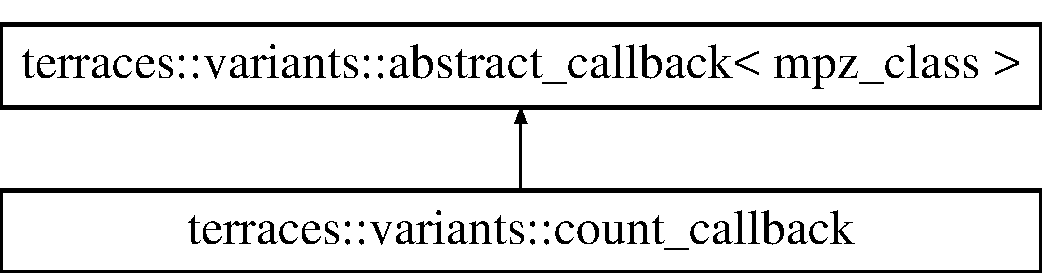
\includegraphics[height=2.000000cm]{classterraces_1_1variants_1_1count__callback}
\end{center}
\end{figure}
\subsection*{Public Types}
\begin{DoxyCompactItemize}
\item 
using \hyperlink{classterraces_1_1variants_1_1count__callback_adb8cc586b7f8d5aeaa4d1d83c36c5cb8}{return\+\_\+type} = \hyperlink{classterraces_1_1variants_1_1abstract__callback_ac1da94f0be306068e89627dc40cd0f3b}{abstract\+\_\+callback\+::result\+\_\+type}
\end{DoxyCompactItemize}
\subsection*{Public Member Functions}
\begin{DoxyCompactItemize}
\item 
\hyperlink{classterraces_1_1variants_1_1count__callback_adb8cc586b7f8d5aeaa4d1d83c36c5cb8}{return\+\_\+type} \hyperlink{classterraces_1_1variants_1_1count__callback_a286a391ba17a1e6e0b2d3d5294c7a4f8}{base\+\_\+one\+\_\+leaf} (\hyperlink{namespaceterraces_adbc33ccb543d1634e96d0eb02e472c77}{index})
\item 
\hyperlink{classterraces_1_1variants_1_1count__callback_adb8cc586b7f8d5aeaa4d1d83c36c5cb8}{return\+\_\+type} \hyperlink{classterraces_1_1variants_1_1count__callback_a4964310381cb80333c4211544a9d91e0}{base\+\_\+two\+\_\+leaves} (\hyperlink{namespaceterraces_adbc33ccb543d1634e96d0eb02e472c77}{index}, \hyperlink{namespaceterraces_adbc33ccb543d1634e96d0eb02e472c77}{index})
\item 
\hyperlink{classterraces_1_1variants_1_1count__callback_adb8cc586b7f8d5aeaa4d1d83c36c5cb8}{return\+\_\+type} \hyperlink{classterraces_1_1variants_1_1count__callback_ad4d7c49a1a82c88db125eaf9241ea8d4}{base\+\_\+unconstrained} (const \hyperlink{namespaceterraces_acc45ec9c561024c50ecbce5b6738ba08}{ranked\+\_\+bitvector} \&leaves)
\item 
\hyperlink{classterraces_1_1variants_1_1count__callback_adb8cc586b7f8d5aeaa4d1d83c36c5cb8}{return\+\_\+type} \hyperlink{classterraces_1_1variants_1_1count__callback_ae0d0708bdde2b61cf4e3df15edda9be7}{null\+\_\+result} ()
\item 
\hyperlink{namespaceterraces_adbc33ccb543d1634e96d0eb02e472c77}{index} \hyperlink{classterraces_1_1variants_1_1count__callback_a5bf31dc18b0ba1ee01d2ae54587db183}{fast\+\_\+return\+\_\+value} (const \hyperlink{classterraces_1_1bipartition__iterator}{bipartition\+\_\+iterator} \&bip\+\_\+it)
\item 
\hyperlink{classterraces_1_1variants_1_1count__callback_adb8cc586b7f8d5aeaa4d1d83c36c5cb8}{return\+\_\+type} \hyperlink{classterraces_1_1variants_1_1count__callback_a9760d7bb4a9681b6cb06f6c5c35b3152}{accumulate} (\hyperlink{classterraces_1_1variants_1_1count__callback_adb8cc586b7f8d5aeaa4d1d83c36c5cb8}{return\+\_\+type} acc, \hyperlink{classterraces_1_1variants_1_1count__callback_adb8cc586b7f8d5aeaa4d1d83c36c5cb8}{return\+\_\+type} val)
\item 
\hyperlink{classterraces_1_1variants_1_1count__callback_adb8cc586b7f8d5aeaa4d1d83c36c5cb8}{return\+\_\+type} \hyperlink{classterraces_1_1variants_1_1count__callback_afb224c2b473fd827ffe7be77365ab947}{combine} (\hyperlink{classterraces_1_1variants_1_1count__callback_adb8cc586b7f8d5aeaa4d1d83c36c5cb8}{return\+\_\+type} left, \hyperlink{classterraces_1_1variants_1_1count__callback_adb8cc586b7f8d5aeaa4d1d83c36c5cb8}{return\+\_\+type} right)
\end{DoxyCompactItemize}


\subsection{Member Typedef Documentation}
\mbox{\Hypertarget{classterraces_1_1variants_1_1count__callback_adb8cc586b7f8d5aeaa4d1d83c36c5cb8}\label{classterraces_1_1variants_1_1count__callback_adb8cc586b7f8d5aeaa4d1d83c36c5cb8}} 
\index{terraces\+::variants\+::count\+\_\+callback@{terraces\+::variants\+::count\+\_\+callback}!return\+\_\+type@{return\+\_\+type}}
\index{return\+\_\+type@{return\+\_\+type}!terraces\+::variants\+::count\+\_\+callback@{terraces\+::variants\+::count\+\_\+callback}}
\subsubsection{\texorpdfstring{return\+\_\+type}{return\_type}}
{\footnotesize\ttfamily using \hyperlink{classterraces_1_1variants_1_1count__callback_adb8cc586b7f8d5aeaa4d1d83c36c5cb8}{terraces\+::variants\+::count\+\_\+callback\+::return\+\_\+type} =  \hyperlink{classterraces_1_1variants_1_1abstract__callback_ac1da94f0be306068e89627dc40cd0f3b}{abstract\+\_\+callback\+::result\+\_\+type}}



\subsection{Member Function Documentation}
\mbox{\Hypertarget{classterraces_1_1variants_1_1count__callback_a9760d7bb4a9681b6cb06f6c5c35b3152}\label{classterraces_1_1variants_1_1count__callback_a9760d7bb4a9681b6cb06f6c5c35b3152}} 
\index{terraces\+::variants\+::count\+\_\+callback@{terraces\+::variants\+::count\+\_\+callback}!accumulate@{accumulate}}
\index{accumulate@{accumulate}!terraces\+::variants\+::count\+\_\+callback@{terraces\+::variants\+::count\+\_\+callback}}
\subsubsection{\texorpdfstring{accumulate()}{accumulate()}}
{\footnotesize\ttfamily \hyperlink{classterraces_1_1variants_1_1count__callback_adb8cc586b7f8d5aeaa4d1d83c36c5cb8}{return\+\_\+type} terraces\+::variants\+::count\+\_\+callback\+::accumulate (\begin{DoxyParamCaption}\item[{\hyperlink{classterraces_1_1variants_1_1count__callback_adb8cc586b7f8d5aeaa4d1d83c36c5cb8}{return\+\_\+type}}]{acc,  }\item[{\hyperlink{classterraces_1_1variants_1_1count__callback_adb8cc586b7f8d5aeaa4d1d83c36c5cb8}{return\+\_\+type}}]{val }\end{DoxyParamCaption})\hspace{0.3cm}{\ttfamily [inline]}}

\mbox{\Hypertarget{classterraces_1_1variants_1_1count__callback_a286a391ba17a1e6e0b2d3d5294c7a4f8}\label{classterraces_1_1variants_1_1count__callback_a286a391ba17a1e6e0b2d3d5294c7a4f8}} 
\index{terraces\+::variants\+::count\+\_\+callback@{terraces\+::variants\+::count\+\_\+callback}!base\+\_\+one\+\_\+leaf@{base\+\_\+one\+\_\+leaf}}
\index{base\+\_\+one\+\_\+leaf@{base\+\_\+one\+\_\+leaf}!terraces\+::variants\+::count\+\_\+callback@{terraces\+::variants\+::count\+\_\+callback}}
\subsubsection{\texorpdfstring{base\+\_\+one\+\_\+leaf()}{base\_one\_leaf()}}
{\footnotesize\ttfamily \hyperlink{classterraces_1_1variants_1_1count__callback_adb8cc586b7f8d5aeaa4d1d83c36c5cb8}{return\+\_\+type} terraces\+::variants\+::count\+\_\+callback\+::base\+\_\+one\+\_\+leaf (\begin{DoxyParamCaption}\item[{\hyperlink{namespaceterraces_adbc33ccb543d1634e96d0eb02e472c77}{index}}]{ }\end{DoxyParamCaption})\hspace{0.3cm}{\ttfamily [inline]}}

\mbox{\Hypertarget{classterraces_1_1variants_1_1count__callback_a4964310381cb80333c4211544a9d91e0}\label{classterraces_1_1variants_1_1count__callback_a4964310381cb80333c4211544a9d91e0}} 
\index{terraces\+::variants\+::count\+\_\+callback@{terraces\+::variants\+::count\+\_\+callback}!base\+\_\+two\+\_\+leaves@{base\+\_\+two\+\_\+leaves}}
\index{base\+\_\+two\+\_\+leaves@{base\+\_\+two\+\_\+leaves}!terraces\+::variants\+::count\+\_\+callback@{terraces\+::variants\+::count\+\_\+callback}}
\subsubsection{\texorpdfstring{base\+\_\+two\+\_\+leaves()}{base\_two\_leaves()}}
{\footnotesize\ttfamily \hyperlink{classterraces_1_1variants_1_1count__callback_adb8cc586b7f8d5aeaa4d1d83c36c5cb8}{return\+\_\+type} terraces\+::variants\+::count\+\_\+callback\+::base\+\_\+two\+\_\+leaves (\begin{DoxyParamCaption}\item[{\hyperlink{namespaceterraces_adbc33ccb543d1634e96d0eb02e472c77}{index}}]{,  }\item[{\hyperlink{namespaceterraces_adbc33ccb543d1634e96d0eb02e472c77}{index}}]{ }\end{DoxyParamCaption})\hspace{0.3cm}{\ttfamily [inline]}}

\mbox{\Hypertarget{classterraces_1_1variants_1_1count__callback_ad4d7c49a1a82c88db125eaf9241ea8d4}\label{classterraces_1_1variants_1_1count__callback_ad4d7c49a1a82c88db125eaf9241ea8d4}} 
\index{terraces\+::variants\+::count\+\_\+callback@{terraces\+::variants\+::count\+\_\+callback}!base\+\_\+unconstrained@{base\+\_\+unconstrained}}
\index{base\+\_\+unconstrained@{base\+\_\+unconstrained}!terraces\+::variants\+::count\+\_\+callback@{terraces\+::variants\+::count\+\_\+callback}}
\subsubsection{\texorpdfstring{base\+\_\+unconstrained()}{base\_unconstrained()}}
{\footnotesize\ttfamily \hyperlink{classterraces_1_1variants_1_1count__callback_adb8cc586b7f8d5aeaa4d1d83c36c5cb8}{return\+\_\+type} terraces\+::variants\+::count\+\_\+callback\+::base\+\_\+unconstrained (\begin{DoxyParamCaption}\item[{const \hyperlink{namespaceterraces_acc45ec9c561024c50ecbce5b6738ba08}{ranked\+\_\+bitvector} \&}]{leaves }\end{DoxyParamCaption})\hspace{0.3cm}{\ttfamily [inline]}}

\mbox{\Hypertarget{classterraces_1_1variants_1_1count__callback_afb224c2b473fd827ffe7be77365ab947}\label{classterraces_1_1variants_1_1count__callback_afb224c2b473fd827ffe7be77365ab947}} 
\index{terraces\+::variants\+::count\+\_\+callback@{terraces\+::variants\+::count\+\_\+callback}!combine@{combine}}
\index{combine@{combine}!terraces\+::variants\+::count\+\_\+callback@{terraces\+::variants\+::count\+\_\+callback}}
\subsubsection{\texorpdfstring{combine()}{combine()}}
{\footnotesize\ttfamily \hyperlink{classterraces_1_1variants_1_1count__callback_adb8cc586b7f8d5aeaa4d1d83c36c5cb8}{return\+\_\+type} terraces\+::variants\+::count\+\_\+callback\+::combine (\begin{DoxyParamCaption}\item[{\hyperlink{classterraces_1_1variants_1_1count__callback_adb8cc586b7f8d5aeaa4d1d83c36c5cb8}{return\+\_\+type}}]{left,  }\item[{\hyperlink{classterraces_1_1variants_1_1count__callback_adb8cc586b7f8d5aeaa4d1d83c36c5cb8}{return\+\_\+type}}]{right }\end{DoxyParamCaption})\hspace{0.3cm}{\ttfamily [inline]}}

\mbox{\Hypertarget{classterraces_1_1variants_1_1count__callback_a5bf31dc18b0ba1ee01d2ae54587db183}\label{classterraces_1_1variants_1_1count__callback_a5bf31dc18b0ba1ee01d2ae54587db183}} 
\index{terraces\+::variants\+::count\+\_\+callback@{terraces\+::variants\+::count\+\_\+callback}!fast\+\_\+return\+\_\+value@{fast\+\_\+return\+\_\+value}}
\index{fast\+\_\+return\+\_\+value@{fast\+\_\+return\+\_\+value}!terraces\+::variants\+::count\+\_\+callback@{terraces\+::variants\+::count\+\_\+callback}}
\subsubsection{\texorpdfstring{fast\+\_\+return\+\_\+value()}{fast\_return\_value()}}
{\footnotesize\ttfamily \hyperlink{namespaceterraces_adbc33ccb543d1634e96d0eb02e472c77}{index} terraces\+::variants\+::count\+\_\+callback\+::fast\+\_\+return\+\_\+value (\begin{DoxyParamCaption}\item[{const \hyperlink{classterraces_1_1bipartition__iterator}{bipartition\+\_\+iterator} \&}]{bip\+\_\+it }\end{DoxyParamCaption})\hspace{0.3cm}{\ttfamily [inline]}}

\mbox{\Hypertarget{classterraces_1_1variants_1_1count__callback_ae0d0708bdde2b61cf4e3df15edda9be7}\label{classterraces_1_1variants_1_1count__callback_ae0d0708bdde2b61cf4e3df15edda9be7}} 
\index{terraces\+::variants\+::count\+\_\+callback@{terraces\+::variants\+::count\+\_\+callback}!null\+\_\+result@{null\+\_\+result}}
\index{null\+\_\+result@{null\+\_\+result}!terraces\+::variants\+::count\+\_\+callback@{terraces\+::variants\+::count\+\_\+callback}}
\subsubsection{\texorpdfstring{null\+\_\+result()}{null\_result()}}
{\footnotesize\ttfamily \hyperlink{classterraces_1_1variants_1_1count__callback_adb8cc586b7f8d5aeaa4d1d83c36c5cb8}{return\+\_\+type} terraces\+::variants\+::count\+\_\+callback\+::null\+\_\+result (\begin{DoxyParamCaption}{ }\end{DoxyParamCaption})\hspace{0.3cm}{\ttfamily [inline]}}



The documentation for this class was generated from the following file\+:\begin{DoxyCompactItemize}
\item 
lib/\hyperlink{supertree__variants_8hpp}{supertree\+\_\+variants.\+hpp}\end{DoxyCompactItemize}

\hypertarget{structterraces_1_1counted__supertree}{}\section{terraces\+:\+:counted\+\_\+supertree Struct Reference}
\label{structterraces_1_1counted__supertree}\index{terraces\+::counted\+\_\+supertree@{terraces\+::counted\+\_\+supertree}}


{\ttfamily \#include $<$trees.\+hpp$>$}

\subsection*{Public Attributes}
\begin{DoxyCompactItemize}
\item 
const \hyperlink{namespaceterraces_adbc33ccb543d1634e96d0eb02e472c77}{index} \hyperlink{structterraces_1_1counted__supertree_a0ba6a52d09a0b572d1821d852a210f11}{count}
\item 
const std\+::string \hyperlink{structterraces_1_1counted__supertree_aa36892e795125017ec7a2efc27bfc673}{supertree}
\end{DoxyCompactItemize}


\subsection{Member Data Documentation}
\mbox{\Hypertarget{structterraces_1_1counted__supertree_a0ba6a52d09a0b572d1821d852a210f11}\label{structterraces_1_1counted__supertree_a0ba6a52d09a0b572d1821d852a210f11}} 
\index{terraces\+::counted\+\_\+supertree@{terraces\+::counted\+\_\+supertree}!count@{count}}
\index{count@{count}!terraces\+::counted\+\_\+supertree@{terraces\+::counted\+\_\+supertree}}
\subsubsection{\texorpdfstring{count}{count}}
{\footnotesize\ttfamily const \hyperlink{namespaceterraces_adbc33ccb543d1634e96d0eb02e472c77}{index} terraces\+::counted\+\_\+supertree\+::count}

\mbox{\Hypertarget{structterraces_1_1counted__supertree_aa36892e795125017ec7a2efc27bfc673}\label{structterraces_1_1counted__supertree_aa36892e795125017ec7a2efc27bfc673}} 
\index{terraces\+::counted\+\_\+supertree@{terraces\+::counted\+\_\+supertree}!supertree@{supertree}}
\index{supertree@{supertree}!terraces\+::counted\+\_\+supertree@{terraces\+::counted\+\_\+supertree}}
\subsubsection{\texorpdfstring{supertree}{supertree}}
{\footnotesize\ttfamily const std\+::string terraces\+::counted\+\_\+supertree\+::supertree}



The documentation for this struct was generated from the following file\+:\begin{DoxyCompactItemize}
\item 
include/terraces/\hyperlink{trees_8hpp}{trees.\+hpp}\end{DoxyCompactItemize}

\hypertarget{classterraces_1_1variants_1_1fast__check__decorator}{}\section{terraces\+:\+:variants\+:\+:fast\+\_\+check\+\_\+decorator$<$ Callback $>$ Class Template Reference}
\label{classterraces_1_1variants_1_1fast__check__decorator}\index{terraces\+::variants\+::fast\+\_\+check\+\_\+decorator$<$ Callback $>$@{terraces\+::variants\+::fast\+\_\+check\+\_\+decorator$<$ Callback $>$}}


{\ttfamily \#include $<$supertree\+\_\+variants.\+hpp$>$}

Inheritance diagram for terraces\+:\+:variants\+:\+:fast\+\_\+check\+\_\+decorator$<$ Callback $>$\+:\begin{figure}[H]
\begin{center}
\leavevmode
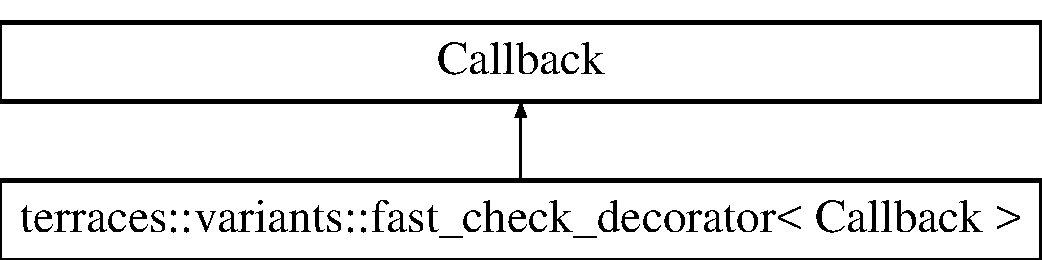
\includegraphics[height=2.000000cm]{classterraces_1_1variants_1_1fast__check__decorator}
\end{center}
\end{figure}
\subsection*{Public Types}
\begin{DoxyCompactItemize}
\item 
using \hyperlink{classterraces_1_1variants_1_1fast__check__decorator_ae6258cfecb5cea22cf0a30ab3c0bbfe9}{return\+\_\+type} = typename Callback\+::result\+\_\+type
\end{DoxyCompactItemize}
\subsection*{Public Member Functions}
\begin{DoxyCompactItemize}
\item 
bool \hyperlink{classterraces_1_1variants_1_1fast__check__decorator_afc5fc595fa03aa85ed65a3741c5a97c0}{fast\+\_\+return} (const \hyperlink{classterraces_1_1bipartition__iterator}{bipartition\+\_\+iterator} \&bip\+\_\+it)
\end{DoxyCompactItemize}


\subsection{Member Typedef Documentation}
\mbox{\Hypertarget{classterraces_1_1variants_1_1fast__check__decorator_ae6258cfecb5cea22cf0a30ab3c0bbfe9}\label{classterraces_1_1variants_1_1fast__check__decorator_ae6258cfecb5cea22cf0a30ab3c0bbfe9}} 
\index{terraces\+::variants\+::fast\+\_\+check\+\_\+decorator@{terraces\+::variants\+::fast\+\_\+check\+\_\+decorator}!return\+\_\+type@{return\+\_\+type}}
\index{return\+\_\+type@{return\+\_\+type}!terraces\+::variants\+::fast\+\_\+check\+\_\+decorator@{terraces\+::variants\+::fast\+\_\+check\+\_\+decorator}}
\subsubsection{\texorpdfstring{return\+\_\+type}{return\_type}}
{\footnotesize\ttfamily template$<$typename Callback $>$ \\
using \hyperlink{classterraces_1_1variants_1_1fast__check__decorator}{terraces\+::variants\+::fast\+\_\+check\+\_\+decorator}$<$ Callback $>$\+::\hyperlink{classterraces_1_1variants_1_1fast__check__decorator_ae6258cfecb5cea22cf0a30ab3c0bbfe9}{return\+\_\+type} =  typename Callback\+::result\+\_\+type}



\subsection{Member Function Documentation}
\mbox{\Hypertarget{classterraces_1_1variants_1_1fast__check__decorator_afc5fc595fa03aa85ed65a3741c5a97c0}\label{classterraces_1_1variants_1_1fast__check__decorator_afc5fc595fa03aa85ed65a3741c5a97c0}} 
\index{terraces\+::variants\+::fast\+\_\+check\+\_\+decorator@{terraces\+::variants\+::fast\+\_\+check\+\_\+decorator}!fast\+\_\+return@{fast\+\_\+return}}
\index{fast\+\_\+return@{fast\+\_\+return}!terraces\+::variants\+::fast\+\_\+check\+\_\+decorator@{terraces\+::variants\+::fast\+\_\+check\+\_\+decorator}}
\subsubsection{\texorpdfstring{fast\+\_\+return()}{fast\_return()}}
{\footnotesize\ttfamily template$<$typename Callback $>$ \\
bool \hyperlink{classterraces_1_1variants_1_1fast__check__decorator}{terraces\+::variants\+::fast\+\_\+check\+\_\+decorator}$<$ Callback $>$\+::fast\+\_\+return (\begin{DoxyParamCaption}\item[{const \hyperlink{classterraces_1_1bipartition__iterator}{bipartition\+\_\+iterator} \&}]{bip\+\_\+it }\end{DoxyParamCaption})\hspace{0.3cm}{\ttfamily [inline]}}



The documentation for this class was generated from the following file\+:\begin{DoxyCompactItemize}
\item 
lib/\hyperlink{supertree__variants_8hpp}{supertree\+\_\+variants.\+hpp}\end{DoxyCompactItemize}

\hypertarget{classterraces_1_1file__open__error}{}\section{terraces\+:\+:file\+\_\+open\+\_\+error Class Reference}
\label{classterraces_1_1file__open__error}\index{terraces\+::file\+\_\+open\+\_\+error@{terraces\+::file\+\_\+open\+\_\+error}}


{\ttfamily \#include $<$errors.\+hpp$>$}

Inheritance diagram for terraces\+:\+:file\+\_\+open\+\_\+error\+:\begin{figure}[H]
\begin{center}
\leavevmode
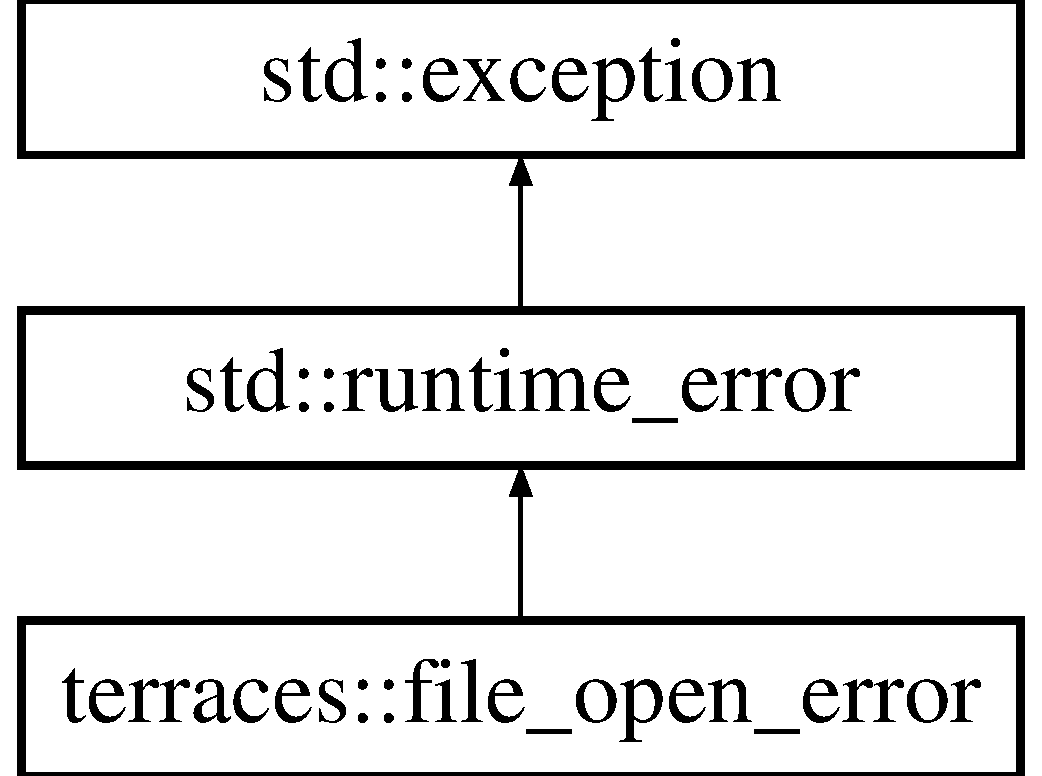
\includegraphics[height=3.000000cm]{classterraces_1_1file__open__error}
\end{center}
\end{figure}


The documentation for this class was generated from the following file\+:\begin{DoxyCompactItemize}
\item 
include/terraces/\hyperlink{errors_8hpp}{errors.\+hpp}\end{DoxyCompactItemize}

\hypertarget{classterraces_1_1utils_1_1free__list}{}\section{terraces\+:\+:utils\+:\+:free\+\_\+list Class Reference}
\label{classterraces_1_1utils_1_1free__list}\index{terraces\+::utils\+::free\+\_\+list@{terraces\+::utils\+::free\+\_\+list}}


{\ttfamily \#include $<$stack\+\_\+allocator.\+hpp$>$}

\subsection*{Public Member Functions}
\begin{DoxyCompactItemize}
\item 
void \hyperlink{classterraces_1_1utils_1_1free__list_a40130edfe36feff64e9ec3de5cc2f769}{push} (\hyperlink{namespaceterraces_1_1utils_a899529841c01a7e7152ac5ef8496c024}{char\+\_\+buffer} ptr)
\item 
\hyperlink{namespaceterraces_1_1utils_a899529841c01a7e7152ac5ef8496c024}{char\+\_\+buffer} \hyperlink{classterraces_1_1utils_1_1free__list_a1a03cbac7b032f831db07d4174f5519e}{pop} ()
\end{DoxyCompactItemize}


\subsection{Member Function Documentation}
\mbox{\Hypertarget{classterraces_1_1utils_1_1free__list_a1a03cbac7b032f831db07d4174f5519e}\label{classterraces_1_1utils_1_1free__list_a1a03cbac7b032f831db07d4174f5519e}} 
\index{terraces\+::utils\+::free\+\_\+list@{terraces\+::utils\+::free\+\_\+list}!pop@{pop}}
\index{pop@{pop}!terraces\+::utils\+::free\+\_\+list@{terraces\+::utils\+::free\+\_\+list}}
\subsubsection{\texorpdfstring{pop()}{pop()}}
{\footnotesize\ttfamily \hyperlink{namespaceterraces_1_1utils_a899529841c01a7e7152ac5ef8496c024}{char\+\_\+buffer} terraces\+::utils\+::free\+\_\+list\+::pop (\begin{DoxyParamCaption}{ }\end{DoxyParamCaption})\hspace{0.3cm}{\ttfamily [inline]}}

\mbox{\Hypertarget{classterraces_1_1utils_1_1free__list_a40130edfe36feff64e9ec3de5cc2f769}\label{classterraces_1_1utils_1_1free__list_a40130edfe36feff64e9ec3de5cc2f769}} 
\index{terraces\+::utils\+::free\+\_\+list@{terraces\+::utils\+::free\+\_\+list}!push@{push}}
\index{push@{push}!terraces\+::utils\+::free\+\_\+list@{terraces\+::utils\+::free\+\_\+list}}
\subsubsection{\texorpdfstring{push()}{push()}}
{\footnotesize\ttfamily void terraces\+::utils\+::free\+\_\+list\+::push (\begin{DoxyParamCaption}\item[{\hyperlink{namespaceterraces_1_1utils_a899529841c01a7e7152ac5ef8496c024}{char\+\_\+buffer}}]{ptr }\end{DoxyParamCaption})\hspace{0.3cm}{\ttfamily [inline]}}



The documentation for this class was generated from the following file\+:\begin{DoxyCompactItemize}
\item 
lib/\hyperlink{stack__allocator_8hpp}{stack\+\_\+allocator.\+hpp}\end{DoxyCompactItemize}

\hypertarget{structterraces_1_1index__array__view}{}\section{terraces\+:\+:index\+\_\+array\+\_\+view Struct Reference}
\label{structterraces_1_1index__array__view}\index{terraces\+::index\+\_\+array\+\_\+view@{terraces\+::index\+\_\+array\+\_\+view}}
\subsection*{Public Member Functions}
\begin{DoxyCompactItemize}
\item 
\hyperlink{namespaceterraces_adbc33ccb543d1634e96d0eb02e472c77}{index} $\ast$ \hyperlink{structterraces_1_1index__array__view_af05408fd685cc32bb368eb8573b0c98d}{begin} () const
\item 
\hyperlink{namespaceterraces_adbc33ccb543d1634e96d0eb02e472c77}{index} $\ast$ \hyperlink{structterraces_1_1index__array__view_aeea66f3e774d119b6be5d473f822568f}{end} () const
\end{DoxyCompactItemize}
\subsection*{Public Attributes}
\begin{DoxyCompactItemize}
\item 
\hyperlink{namespaceterraces_adbc33ccb543d1634e96d0eb02e472c77}{index} $\ast$ \hyperlink{structterraces_1_1index__array__view_a0ebf54edfffe71f8771fb7f77dcb811e}{\+\_\+begin}
\item 
\hyperlink{namespaceterraces_adbc33ccb543d1634e96d0eb02e472c77}{index} $\ast$ \hyperlink{structterraces_1_1index__array__view_ad12ad0aa47e15385e01b5b993de729e2}{\+\_\+end}
\end{DoxyCompactItemize}


\subsection{Member Function Documentation}
\mbox{\Hypertarget{structterraces_1_1index__array__view_af05408fd685cc32bb368eb8573b0c98d}\label{structterraces_1_1index__array__view_af05408fd685cc32bb368eb8573b0c98d}} 
\index{terraces\+::index\+\_\+array\+\_\+view@{terraces\+::index\+\_\+array\+\_\+view}!begin@{begin}}
\index{begin@{begin}!terraces\+::index\+\_\+array\+\_\+view@{terraces\+::index\+\_\+array\+\_\+view}}
\subsubsection{\texorpdfstring{begin()}{begin()}}
{\footnotesize\ttfamily \hyperlink{namespaceterraces_adbc33ccb543d1634e96d0eb02e472c77}{index}$\ast$ terraces\+::index\+\_\+array\+\_\+view\+::begin (\begin{DoxyParamCaption}{ }\end{DoxyParamCaption}) const\hspace{0.3cm}{\ttfamily [inline]}}

\mbox{\Hypertarget{structterraces_1_1index__array__view_aeea66f3e774d119b6be5d473f822568f}\label{structterraces_1_1index__array__view_aeea66f3e774d119b6be5d473f822568f}} 
\index{terraces\+::index\+\_\+array\+\_\+view@{terraces\+::index\+\_\+array\+\_\+view}!end@{end}}
\index{end@{end}!terraces\+::index\+\_\+array\+\_\+view@{terraces\+::index\+\_\+array\+\_\+view}}
\subsubsection{\texorpdfstring{end()}{end()}}
{\footnotesize\ttfamily \hyperlink{namespaceterraces_adbc33ccb543d1634e96d0eb02e472c77}{index}$\ast$ terraces\+::index\+\_\+array\+\_\+view\+::end (\begin{DoxyParamCaption}{ }\end{DoxyParamCaption}) const\hspace{0.3cm}{\ttfamily [inline]}}



\subsection{Member Data Documentation}
\mbox{\Hypertarget{structterraces_1_1index__array__view_a0ebf54edfffe71f8771fb7f77dcb811e}\label{structterraces_1_1index__array__view_a0ebf54edfffe71f8771fb7f77dcb811e}} 
\index{terraces\+::index\+\_\+array\+\_\+view@{terraces\+::index\+\_\+array\+\_\+view}!\+\_\+begin@{\+\_\+begin}}
\index{\+\_\+begin@{\+\_\+begin}!terraces\+::index\+\_\+array\+\_\+view@{terraces\+::index\+\_\+array\+\_\+view}}
\subsubsection{\texorpdfstring{\+\_\+begin}{\_begin}}
{\footnotesize\ttfamily \hyperlink{namespaceterraces_adbc33ccb543d1634e96d0eb02e472c77}{index}$\ast$ terraces\+::index\+\_\+array\+\_\+view\+::\+\_\+begin}

\mbox{\Hypertarget{structterraces_1_1index__array__view_ad12ad0aa47e15385e01b5b993de729e2}\label{structterraces_1_1index__array__view_ad12ad0aa47e15385e01b5b993de729e2}} 
\index{terraces\+::index\+\_\+array\+\_\+view@{terraces\+::index\+\_\+array\+\_\+view}!\+\_\+end@{\+\_\+end}}
\index{\+\_\+end@{\+\_\+end}!terraces\+::index\+\_\+array\+\_\+view@{terraces\+::index\+\_\+array\+\_\+view}}
\subsubsection{\texorpdfstring{\+\_\+end}{\_end}}
{\footnotesize\ttfamily \hyperlink{namespaceterraces_adbc33ccb543d1634e96d0eb02e472c77}{index}$\ast$ terraces\+::index\+\_\+array\+\_\+view\+::\+\_\+end}



The documentation for this struct was generated from the following file\+:\begin{DoxyCompactItemize}
\item 
lib/\hyperlink{multitree_8cpp}{multitree.\+cpp}\end{DoxyCompactItemize}

\hypertarget{structterraces_1_1multitree__nodes_1_1inner__node}{}\section{terraces\+:\+:multitree\+\_\+nodes\+:\+:inner\+\_\+node Struct Reference}
\label{structterraces_1_1multitree__nodes_1_1inner__node}\index{terraces\+::multitree\+\_\+nodes\+::inner\+\_\+node@{terraces\+::multitree\+\_\+nodes\+::inner\+\_\+node}}


{\ttfamily \#include $<$multitree.\+hpp$>$}

\subsection*{Public Attributes}
\begin{DoxyCompactItemize}
\item 
\hyperlink{structterraces_1_1multitree__node}{multitree\+\_\+node} $\ast$ \hyperlink{structterraces_1_1multitree__nodes_1_1inner__node_af0f33b9c24c2c273e714db3cd1ab6afd}{left}
\item 
\hyperlink{structterraces_1_1multitree__node}{multitree\+\_\+node} $\ast$ \hyperlink{structterraces_1_1multitree__nodes_1_1inner__node_a987c6beaaf17adc09dc8e2366986ad61}{right}
\end{DoxyCompactItemize}


\subsection{Member Data Documentation}
\mbox{\Hypertarget{structterraces_1_1multitree__nodes_1_1inner__node_af0f33b9c24c2c273e714db3cd1ab6afd}\label{structterraces_1_1multitree__nodes_1_1inner__node_af0f33b9c24c2c273e714db3cd1ab6afd}} 
\index{terraces\+::multitree\+\_\+nodes\+::inner\+\_\+node@{terraces\+::multitree\+\_\+nodes\+::inner\+\_\+node}!left@{left}}
\index{left@{left}!terraces\+::multitree\+\_\+nodes\+::inner\+\_\+node@{terraces\+::multitree\+\_\+nodes\+::inner\+\_\+node}}
\subsubsection{\texorpdfstring{left}{left}}
{\footnotesize\ttfamily \hyperlink{structterraces_1_1multitree__node}{multitree\+\_\+node}$\ast$ terraces\+::multitree\+\_\+nodes\+::inner\+\_\+node\+::left}

\mbox{\Hypertarget{structterraces_1_1multitree__nodes_1_1inner__node_a987c6beaaf17adc09dc8e2366986ad61}\label{structterraces_1_1multitree__nodes_1_1inner__node_a987c6beaaf17adc09dc8e2366986ad61}} 
\index{terraces\+::multitree\+\_\+nodes\+::inner\+\_\+node@{terraces\+::multitree\+\_\+nodes\+::inner\+\_\+node}!right@{right}}
\index{right@{right}!terraces\+::multitree\+\_\+nodes\+::inner\+\_\+node@{terraces\+::multitree\+\_\+nodes\+::inner\+\_\+node}}
\subsubsection{\texorpdfstring{right}{right}}
{\footnotesize\ttfamily \hyperlink{structterraces_1_1multitree__node}{multitree\+\_\+node}$\ast$ terraces\+::multitree\+\_\+nodes\+::inner\+\_\+node\+::right}



The documentation for this struct was generated from the following file\+:\begin{DoxyCompactItemize}
\item 
include/terraces/\hyperlink{multitree_8hpp}{multitree.\+hpp}\end{DoxyCompactItemize}

\hypertarget{structinput__data}{}\section{input\+\_\+data Struct Reference}
\label{structinput__data}\index{input\+\_\+data@{input\+\_\+data}}


{\ttfamily \#include $<$input\+\_\+parser.\+h$>$}

\subsection*{Public Attributes}
\begin{DoxyCompactItemize}
\item 
size\+\_\+t \hyperlink{structinput__data_a10d4f562a6b9dbda373a6fbe9a99e9fe}{number\+\_\+of\+\_\+species}
\item 
size\+\_\+t \hyperlink{structinput__data_ae07405c95174763dd88371d85b6d35a3}{number\+\_\+of\+\_\+partitions}
\item 
unsigned char $\ast$ \hyperlink{structinput__data_adb15938eeec23b8e78af79c8379f8432}{matrix}
\item 
char $\ast$$\ast$ \hyperlink{structinput__data_a3e32e1d152e8c5d245f2ef4fb348a575}{names}
\end{DoxyCompactItemize}


\subsection{Member Data Documentation}
\mbox{\Hypertarget{structinput__data_adb15938eeec23b8e78af79c8379f8432}\label{structinput__data_adb15938eeec23b8e78af79c8379f8432}} 
\index{input\+\_\+data@{input\+\_\+data}!matrix@{matrix}}
\index{matrix@{matrix}!input\+\_\+data@{input\+\_\+data}}
\subsubsection{\texorpdfstring{matrix}{matrix}}
{\footnotesize\ttfamily unsigned char$\ast$ input\+\_\+data\+::matrix}

\mbox{\Hypertarget{structinput__data_a3e32e1d152e8c5d245f2ef4fb348a575}\label{structinput__data_a3e32e1d152e8c5d245f2ef4fb348a575}} 
\index{input\+\_\+data@{input\+\_\+data}!names@{names}}
\index{names@{names}!input\+\_\+data@{input\+\_\+data}}
\subsubsection{\texorpdfstring{names}{names}}
{\footnotesize\ttfamily char$\ast$$\ast$ input\+\_\+data\+::names}

\mbox{\Hypertarget{structinput__data_ae07405c95174763dd88371d85b6d35a3}\label{structinput__data_ae07405c95174763dd88371d85b6d35a3}} 
\index{input\+\_\+data@{input\+\_\+data}!number\+\_\+of\+\_\+partitions@{number\+\_\+of\+\_\+partitions}}
\index{number\+\_\+of\+\_\+partitions@{number\+\_\+of\+\_\+partitions}!input\+\_\+data@{input\+\_\+data}}
\subsubsection{\texorpdfstring{number\+\_\+of\+\_\+partitions}{number\_of\_partitions}}
{\footnotesize\ttfamily size\+\_\+t input\+\_\+data\+::number\+\_\+of\+\_\+partitions}

\mbox{\Hypertarget{structinput__data_a10d4f562a6b9dbda373a6fbe9a99e9fe}\label{structinput__data_a10d4f562a6b9dbda373a6fbe9a99e9fe}} 
\index{input\+\_\+data@{input\+\_\+data}!number\+\_\+of\+\_\+species@{number\+\_\+of\+\_\+species}}
\index{number\+\_\+of\+\_\+species@{number\+\_\+of\+\_\+species}!input\+\_\+data@{input\+\_\+data}}
\subsubsection{\texorpdfstring{number\+\_\+of\+\_\+species}{number\_of\_species}}
{\footnotesize\ttfamily size\+\_\+t input\+\_\+data\+::number\+\_\+of\+\_\+species}



The documentation for this struct was generated from the following file\+:\begin{DoxyCompactItemize}
\item 
alexis\+\_\+samples/\hyperlink{input__parser_8h}{input\+\_\+parser.\+h}\end{DoxyCompactItemize}

\hypertarget{structterraces_1_1multitree__nodes_1_1leaves}{}\section{terraces\+:\+:multitree\+\_\+nodes\+:\+:leaves Struct Reference}
\label{structterraces_1_1multitree__nodes_1_1leaves}\index{terraces\+::multitree\+\_\+nodes\+::leaves@{terraces\+::multitree\+\_\+nodes\+::leaves}}


{\ttfamily \#include $<$multitree.\+hpp$>$}

\subsection*{Public Attributes}
\begin{DoxyCompactItemize}
\item 
\hyperlink{namespaceterraces_adbc33ccb543d1634e96d0eb02e472c77}{index} \hyperlink{structterraces_1_1multitree__nodes_1_1leaves_ae5a944e1e6db1e1127c375f5f670f9cf}{left\+\_\+leaf}
\item 
\hyperlink{namespaceterraces_adbc33ccb543d1634e96d0eb02e472c77}{index} \hyperlink{structterraces_1_1multitree__nodes_1_1leaves_a0596c6b5bed8da9d5cb60fcf6133b75b}{right\+\_\+leaf}
\end{DoxyCompactItemize}


\subsection{Member Data Documentation}
\mbox{\Hypertarget{structterraces_1_1multitree__nodes_1_1leaves_ae5a944e1e6db1e1127c375f5f670f9cf}\label{structterraces_1_1multitree__nodes_1_1leaves_ae5a944e1e6db1e1127c375f5f670f9cf}} 
\index{terraces\+::multitree\+\_\+nodes\+::leaves@{terraces\+::multitree\+\_\+nodes\+::leaves}!left\+\_\+leaf@{left\+\_\+leaf}}
\index{left\+\_\+leaf@{left\+\_\+leaf}!terraces\+::multitree\+\_\+nodes\+::leaves@{terraces\+::multitree\+\_\+nodes\+::leaves}}
\subsubsection{\texorpdfstring{left\+\_\+leaf}{left\_leaf}}
{\footnotesize\ttfamily \hyperlink{namespaceterraces_adbc33ccb543d1634e96d0eb02e472c77}{index} terraces\+::multitree\+\_\+nodes\+::leaves\+::left\+\_\+leaf}

\mbox{\Hypertarget{structterraces_1_1multitree__nodes_1_1leaves_a0596c6b5bed8da9d5cb60fcf6133b75b}\label{structterraces_1_1multitree__nodes_1_1leaves_a0596c6b5bed8da9d5cb60fcf6133b75b}} 
\index{terraces\+::multitree\+\_\+nodes\+::leaves@{terraces\+::multitree\+\_\+nodes\+::leaves}!right\+\_\+leaf@{right\+\_\+leaf}}
\index{right\+\_\+leaf@{right\+\_\+leaf}!terraces\+::multitree\+\_\+nodes\+::leaves@{terraces\+::multitree\+\_\+nodes\+::leaves}}
\subsubsection{\texorpdfstring{right\+\_\+leaf}{right\_leaf}}
{\footnotesize\ttfamily \hyperlink{namespaceterraces_adbc33ccb543d1634e96d0eb02e472c77}{index} terraces\+::multitree\+\_\+nodes\+::leaves\+::right\+\_\+leaf}



The documentation for this struct was generated from the following file\+:\begin{DoxyCompactItemize}
\item 
include/terraces/\hyperlink{multitree_8hpp}{multitree.\+hpp}\end{DoxyCompactItemize}

\hypertarget{classterraces_1_1debug_1_1variants_1_1logging__decorator}{}\section{terraces\+:\+:debug\+:\+:variants\+:\+:logging\+\_\+decorator$<$ Callback $>$ Class Template Reference}
\label{classterraces_1_1debug_1_1variants_1_1logging__decorator}\index{terraces\+::debug\+::variants\+::logging\+\_\+decorator$<$ Callback $>$@{terraces\+::debug\+::variants\+::logging\+\_\+decorator$<$ Callback $>$}}


{\ttfamily \#include $<$supertree\+\_\+variants\+\_\+debug.\+hpp$>$}

Inheritance diagram for terraces\+:\+:debug\+:\+:variants\+:\+:logging\+\_\+decorator$<$ Callback $>$\+:\begin{figure}[H]
\begin{center}
\leavevmode
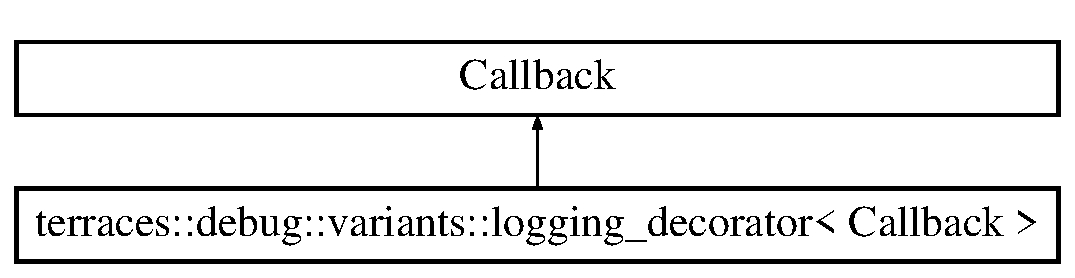
\includegraphics[height=2.000000cm]{classterraces_1_1debug_1_1variants_1_1logging__decorator}
\end{center}
\end{figure}
\subsection*{Public Types}
\begin{DoxyCompactItemize}
\item 
using \hyperlink{classterraces_1_1debug_1_1variants_1_1logging__decorator_a7c08c8ede1f8c884a3bab0437b244f55}{result\+\_\+type} = typename Callback\+::result\+\_\+type
\end{DoxyCompactItemize}
\subsection*{Public Member Functions}
\begin{DoxyCompactItemize}
\item 
{\footnotesize template$<$typename... Args$>$ }\\\hyperlink{classterraces_1_1debug_1_1variants_1_1logging__decorator_a6e9f97ef90017d53d69241a9b827014e}{logging\+\_\+decorator} (Args \&\&... args, std\+::ostream \&output, const \hyperlink{namespaceterraces_a4ef0217fe5aed881737d9bc5a8d45dca}{name\+\_\+map} \&names)
\item 
void \hyperlink{classterraces_1_1debug_1_1variants_1_1logging__decorator_a05818c97704f093630e84b915b58a5cd}{enter} (const \hyperlink{namespaceterraces_acc45ec9c561024c50ecbce5b6738ba08}{ranked\+\_\+bitvector} \&leaves)
\item 
\hyperlink{classterraces_1_1debug_1_1variants_1_1logging__decorator_a7c08c8ede1f8c884a3bab0437b244f55}{result\+\_\+type} \hyperlink{classterraces_1_1debug_1_1variants_1_1logging__decorator_abd1db25829d4a60328582e094d36c4fd}{begin\+\_\+iteration} (const \hyperlink{classterraces_1_1bipartition__iterator}{bipartition\+\_\+iterator} \&bip\+\_\+it, const \hyperlink{namespaceterraces_a1b526fb554dff829f7ad51eb21d5ed06}{bitvector} \&c\+\_\+occ, const \hyperlink{namespaceterraces_a6f603ffd30ed4d902fce6424492e0581}{constraints} \&c)
\item 
void \hyperlink{classterraces_1_1debug_1_1variants_1_1logging__decorator_abf7256cde9b9aada061a80c8dd7a011f}{step\+\_\+iteration} (const \hyperlink{classterraces_1_1bipartition__iterator}{bipartition\+\_\+iterator} \&bip\+\_\+it)
\item 
void \hyperlink{classterraces_1_1debug_1_1variants_1_1logging__decorator_aed1d3afe4d25a5b08be18c8576b98dd8}{finish\+\_\+iteration} ()
\item 
\hyperlink{classterraces_1_1debug_1_1variants_1_1logging__decorator_a7c08c8ede1f8c884a3bab0437b244f55}{result\+\_\+type} \hyperlink{classterraces_1_1debug_1_1variants_1_1logging__decorator_a8279aabed27469c45219527121f5948b}{exit} (\hyperlink{classterraces_1_1debug_1_1variants_1_1logging__decorator_a7c08c8ede1f8c884a3bab0437b244f55}{result\+\_\+type} result)
\end{DoxyCompactItemize}


\subsection{Member Typedef Documentation}
\mbox{\Hypertarget{classterraces_1_1debug_1_1variants_1_1logging__decorator_a7c08c8ede1f8c884a3bab0437b244f55}\label{classterraces_1_1debug_1_1variants_1_1logging__decorator_a7c08c8ede1f8c884a3bab0437b244f55}} 
\index{terraces\+::debug\+::variants\+::logging\+\_\+decorator@{terraces\+::debug\+::variants\+::logging\+\_\+decorator}!result\+\_\+type@{result\+\_\+type}}
\index{result\+\_\+type@{result\+\_\+type}!terraces\+::debug\+::variants\+::logging\+\_\+decorator@{terraces\+::debug\+::variants\+::logging\+\_\+decorator}}
\subsubsection{\texorpdfstring{result\+\_\+type}{result\_type}}
{\footnotesize\ttfamily template$<$typename Callback $>$ \\
using \hyperlink{classterraces_1_1debug_1_1variants_1_1logging__decorator}{terraces\+::debug\+::variants\+::logging\+\_\+decorator}$<$ Callback $>$\+::\hyperlink{classterraces_1_1debug_1_1variants_1_1logging__decorator_a7c08c8ede1f8c884a3bab0437b244f55}{result\+\_\+type} =  typename Callback\+::result\+\_\+type}



\subsection{Constructor \& Destructor Documentation}
\mbox{\Hypertarget{classterraces_1_1debug_1_1variants_1_1logging__decorator_a6e9f97ef90017d53d69241a9b827014e}\label{classterraces_1_1debug_1_1variants_1_1logging__decorator_a6e9f97ef90017d53d69241a9b827014e}} 
\index{terraces\+::debug\+::variants\+::logging\+\_\+decorator@{terraces\+::debug\+::variants\+::logging\+\_\+decorator}!logging\+\_\+decorator@{logging\+\_\+decorator}}
\index{logging\+\_\+decorator@{logging\+\_\+decorator}!terraces\+::debug\+::variants\+::logging\+\_\+decorator@{terraces\+::debug\+::variants\+::logging\+\_\+decorator}}
\subsubsection{\texorpdfstring{logging\+\_\+decorator()}{logging\_decorator()}}
{\footnotesize\ttfamily template$<$typename Callback $>$ \\
template$<$typename... Args$>$ \\
\hyperlink{classterraces_1_1debug_1_1variants_1_1logging__decorator}{terraces\+::debug\+::variants\+::logging\+\_\+decorator}$<$ Callback $>$\+::\hyperlink{classterraces_1_1debug_1_1variants_1_1logging__decorator}{logging\+\_\+decorator} (\begin{DoxyParamCaption}\item[{Args \&\&...}]{args,  }\item[{std\+::ostream \&}]{output,  }\item[{const \hyperlink{namespaceterraces_a4ef0217fe5aed881737d9bc5a8d45dca}{name\+\_\+map} \&}]{names }\end{DoxyParamCaption})\hspace{0.3cm}{\ttfamily [inline]}}



\subsection{Member Function Documentation}
\mbox{\Hypertarget{classterraces_1_1debug_1_1variants_1_1logging__decorator_abd1db25829d4a60328582e094d36c4fd}\label{classterraces_1_1debug_1_1variants_1_1logging__decorator_abd1db25829d4a60328582e094d36c4fd}} 
\index{terraces\+::debug\+::variants\+::logging\+\_\+decorator@{terraces\+::debug\+::variants\+::logging\+\_\+decorator}!begin\+\_\+iteration@{begin\+\_\+iteration}}
\index{begin\+\_\+iteration@{begin\+\_\+iteration}!terraces\+::debug\+::variants\+::logging\+\_\+decorator@{terraces\+::debug\+::variants\+::logging\+\_\+decorator}}
\subsubsection{\texorpdfstring{begin\+\_\+iteration()}{begin\_iteration()}}
{\footnotesize\ttfamily template$<$typename Callback $>$ \\
\hyperlink{classterraces_1_1debug_1_1variants_1_1logging__decorator_a7c08c8ede1f8c884a3bab0437b244f55}{result\+\_\+type} \hyperlink{classterraces_1_1debug_1_1variants_1_1logging__decorator}{terraces\+::debug\+::variants\+::logging\+\_\+decorator}$<$ Callback $>$\+::begin\+\_\+iteration (\begin{DoxyParamCaption}\item[{const \hyperlink{classterraces_1_1bipartition__iterator}{bipartition\+\_\+iterator} \&}]{bip\+\_\+it,  }\item[{const \hyperlink{namespaceterraces_a1b526fb554dff829f7ad51eb21d5ed06}{bitvector} \&}]{c\+\_\+occ,  }\item[{const \hyperlink{namespaceterraces_a6f603ffd30ed4d902fce6424492e0581}{constraints} \&}]{c }\end{DoxyParamCaption})\hspace{0.3cm}{\ttfamily [inline]}}

\mbox{\Hypertarget{classterraces_1_1debug_1_1variants_1_1logging__decorator_a05818c97704f093630e84b915b58a5cd}\label{classterraces_1_1debug_1_1variants_1_1logging__decorator_a05818c97704f093630e84b915b58a5cd}} 
\index{terraces\+::debug\+::variants\+::logging\+\_\+decorator@{terraces\+::debug\+::variants\+::logging\+\_\+decorator}!enter@{enter}}
\index{enter@{enter}!terraces\+::debug\+::variants\+::logging\+\_\+decorator@{terraces\+::debug\+::variants\+::logging\+\_\+decorator}}
\subsubsection{\texorpdfstring{enter()}{enter()}}
{\footnotesize\ttfamily template$<$typename Callback $>$ \\
void \hyperlink{classterraces_1_1debug_1_1variants_1_1logging__decorator}{terraces\+::debug\+::variants\+::logging\+\_\+decorator}$<$ Callback $>$\+::enter (\begin{DoxyParamCaption}\item[{const \hyperlink{namespaceterraces_acc45ec9c561024c50ecbce5b6738ba08}{ranked\+\_\+bitvector} \&}]{leaves }\end{DoxyParamCaption})\hspace{0.3cm}{\ttfamily [inline]}}

\mbox{\Hypertarget{classterraces_1_1debug_1_1variants_1_1logging__decorator_a8279aabed27469c45219527121f5948b}\label{classterraces_1_1debug_1_1variants_1_1logging__decorator_a8279aabed27469c45219527121f5948b}} 
\index{terraces\+::debug\+::variants\+::logging\+\_\+decorator@{terraces\+::debug\+::variants\+::logging\+\_\+decorator}!exit@{exit}}
\index{exit@{exit}!terraces\+::debug\+::variants\+::logging\+\_\+decorator@{terraces\+::debug\+::variants\+::logging\+\_\+decorator}}
\subsubsection{\texorpdfstring{exit()}{exit()}}
{\footnotesize\ttfamily template$<$typename Callback $>$ \\
\hyperlink{classterraces_1_1debug_1_1variants_1_1logging__decorator_a7c08c8ede1f8c884a3bab0437b244f55}{result\+\_\+type} \hyperlink{classterraces_1_1debug_1_1variants_1_1logging__decorator}{terraces\+::debug\+::variants\+::logging\+\_\+decorator}$<$ Callback $>$\+::exit (\begin{DoxyParamCaption}\item[{\hyperlink{classterraces_1_1debug_1_1variants_1_1logging__decorator_a7c08c8ede1f8c884a3bab0437b244f55}{result\+\_\+type}}]{result }\end{DoxyParamCaption})\hspace{0.3cm}{\ttfamily [inline]}}

\mbox{\Hypertarget{classterraces_1_1debug_1_1variants_1_1logging__decorator_aed1d3afe4d25a5b08be18c8576b98dd8}\label{classterraces_1_1debug_1_1variants_1_1logging__decorator_aed1d3afe4d25a5b08be18c8576b98dd8}} 
\index{terraces\+::debug\+::variants\+::logging\+\_\+decorator@{terraces\+::debug\+::variants\+::logging\+\_\+decorator}!finish\+\_\+iteration@{finish\+\_\+iteration}}
\index{finish\+\_\+iteration@{finish\+\_\+iteration}!terraces\+::debug\+::variants\+::logging\+\_\+decorator@{terraces\+::debug\+::variants\+::logging\+\_\+decorator}}
\subsubsection{\texorpdfstring{finish\+\_\+iteration()}{finish\_iteration()}}
{\footnotesize\ttfamily template$<$typename Callback $>$ \\
void \hyperlink{classterraces_1_1debug_1_1variants_1_1logging__decorator}{terraces\+::debug\+::variants\+::logging\+\_\+decorator}$<$ Callback $>$\+::finish\+\_\+iteration (\begin{DoxyParamCaption}{ }\end{DoxyParamCaption})\hspace{0.3cm}{\ttfamily [inline]}}

\mbox{\Hypertarget{classterraces_1_1debug_1_1variants_1_1logging__decorator_abf7256cde9b9aada061a80c8dd7a011f}\label{classterraces_1_1debug_1_1variants_1_1logging__decorator_abf7256cde9b9aada061a80c8dd7a011f}} 
\index{terraces\+::debug\+::variants\+::logging\+\_\+decorator@{terraces\+::debug\+::variants\+::logging\+\_\+decorator}!step\+\_\+iteration@{step\+\_\+iteration}}
\index{step\+\_\+iteration@{step\+\_\+iteration}!terraces\+::debug\+::variants\+::logging\+\_\+decorator@{terraces\+::debug\+::variants\+::logging\+\_\+decorator}}
\subsubsection{\texorpdfstring{step\+\_\+iteration()}{step\_iteration()}}
{\footnotesize\ttfamily template$<$typename Callback $>$ \\
void \hyperlink{classterraces_1_1debug_1_1variants_1_1logging__decorator}{terraces\+::debug\+::variants\+::logging\+\_\+decorator}$<$ Callback $>$\+::step\+\_\+iteration (\begin{DoxyParamCaption}\item[{const \hyperlink{classterraces_1_1bipartition__iterator}{bipartition\+\_\+iterator} \&}]{bip\+\_\+it }\end{DoxyParamCaption})\hspace{0.3cm}{\ttfamily [inline]}}



The documentation for this class was generated from the following file\+:\begin{DoxyCompactItemize}
\item 
lib/\hyperlink{supertree__variants__debug_8hpp}{supertree\+\_\+variants\+\_\+debug.\+hpp}\end{DoxyCompactItemize}

\hypertarget{structmissingData}{}\section{missing\+Data Struct Reference}
\label{structmissingData}\index{missing\+Data@{missing\+Data}}


{\ttfamily \#include $<$terraces.\+h$>$}

\subsection*{Public Attributes}
\begin{DoxyCompactItemize}
\item 
size\+\_\+t \hyperlink{structmissingData_a00557e059d863ca52d69e5e7c6902bb5}{number\+Of\+Species}
\item 
size\+\_\+t \hyperlink{structmissingData_ad72067004d4880edb70f5c1e34f9f89a}{number\+Of\+Partitions}
\item 
unsigned char $\ast$ \hyperlink{structmissingData_a1eca07c43d1fedb1db96890dd8c4c804}{missing\+Data\+Matrix}
\item 
char $\ast$$\ast$ \hyperlink{structmissingData_af6894ef72fad6a289101c37230b9a5f6}{species\+Names}
\item 
bool \hyperlink{structmissingData_a50d97283cf83e155a2517e1951c753d1}{allocated\+Name\+Array}
\end{DoxyCompactItemize}


\subsection{Member Data Documentation}
\mbox{\Hypertarget{structmissingData_a50d97283cf83e155a2517e1951c753d1}\label{structmissingData_a50d97283cf83e155a2517e1951c753d1}} 
\index{missing\+Data@{missing\+Data}!allocated\+Name\+Array@{allocated\+Name\+Array}}
\index{allocated\+Name\+Array@{allocated\+Name\+Array}!missing\+Data@{missing\+Data}}
\subsubsection{\texorpdfstring{allocated\+Name\+Array}{allocatedNameArray}}
{\footnotesize\ttfamily bool missing\+Data\+::allocated\+Name\+Array}

\mbox{\Hypertarget{structmissingData_a1eca07c43d1fedb1db96890dd8c4c804}\label{structmissingData_a1eca07c43d1fedb1db96890dd8c4c804}} 
\index{missing\+Data@{missing\+Data}!missing\+Data\+Matrix@{missing\+Data\+Matrix}}
\index{missing\+Data\+Matrix@{missing\+Data\+Matrix}!missing\+Data@{missing\+Data}}
\subsubsection{\texorpdfstring{missing\+Data\+Matrix}{missingDataMatrix}}
{\footnotesize\ttfamily unsigned char$\ast$ missing\+Data\+::missing\+Data\+Matrix}

\mbox{\Hypertarget{structmissingData_ad72067004d4880edb70f5c1e34f9f89a}\label{structmissingData_ad72067004d4880edb70f5c1e34f9f89a}} 
\index{missing\+Data@{missing\+Data}!number\+Of\+Partitions@{number\+Of\+Partitions}}
\index{number\+Of\+Partitions@{number\+Of\+Partitions}!missing\+Data@{missing\+Data}}
\subsubsection{\texorpdfstring{number\+Of\+Partitions}{numberOfPartitions}}
{\footnotesize\ttfamily size\+\_\+t missing\+Data\+::number\+Of\+Partitions}

\mbox{\Hypertarget{structmissingData_a00557e059d863ca52d69e5e7c6902bb5}\label{structmissingData_a00557e059d863ca52d69e5e7c6902bb5}} 
\index{missing\+Data@{missing\+Data}!number\+Of\+Species@{number\+Of\+Species}}
\index{number\+Of\+Species@{number\+Of\+Species}!missing\+Data@{missing\+Data}}
\subsubsection{\texorpdfstring{number\+Of\+Species}{numberOfSpecies}}
{\footnotesize\ttfamily size\+\_\+t missing\+Data\+::number\+Of\+Species}

\mbox{\Hypertarget{structmissingData_af6894ef72fad6a289101c37230b9a5f6}\label{structmissingData_af6894ef72fad6a289101c37230b9a5f6}} 
\index{missing\+Data@{missing\+Data}!species\+Names@{species\+Names}}
\index{species\+Names@{species\+Names}!missing\+Data@{missing\+Data}}
\subsubsection{\texorpdfstring{species\+Names}{speciesNames}}
{\footnotesize\ttfamily char$\ast$$\ast$ missing\+Data\+::species\+Names}



The documentation for this struct was generated from the following file\+:\begin{DoxyCompactItemize}
\item 
alexis\+\_\+samples/\hyperlink{terraces_8h}{terraces.\+h}\end{DoxyCompactItemize}

\hypertarget{classterraces_1_1variants_1_1multitree__callback}{}\section{terraces\+:\+:variants\+:\+:multitree\+\_\+callback Class Reference}
\label{classterraces_1_1variants_1_1multitree__callback}\index{terraces\+::variants\+::multitree\+\_\+callback@{terraces\+::variants\+::multitree\+\_\+callback}}


{\ttfamily \#include $<$supertree\+\_\+variants\+\_\+multitree.\+hpp$>$}

Inheritance diagram for terraces\+:\+:variants\+:\+:multitree\+\_\+callback\+:\begin{figure}[H]
\begin{center}
\leavevmode
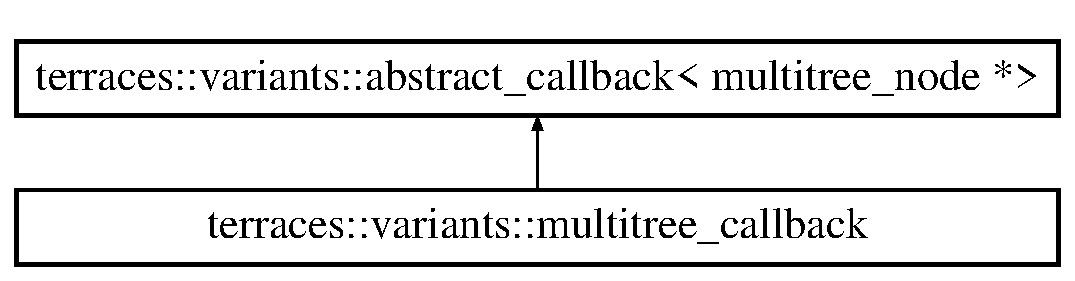
\includegraphics[height=2.000000cm]{classterraces_1_1variants_1_1multitree__callback}
\end{center}
\end{figure}
\subsection*{Public Types}
\begin{DoxyCompactItemize}
\item 
using \hyperlink{classterraces_1_1variants_1_1multitree__callback_a31341dbe798daa06859cd3e0ab354bf1}{return\+\_\+type} = \hyperlink{structterraces_1_1multitree__node}{multitree\+\_\+node} $\ast$
\end{DoxyCompactItemize}
\subsection*{Public Member Functions}
\begin{DoxyCompactItemize}
\item 
\hyperlink{classterraces_1_1variants_1_1multitree__callback_a31341dbe798daa06859cd3e0ab354bf1}{return\+\_\+type} \hyperlink{classterraces_1_1variants_1_1multitree__callback_ae91d72a91413b048a2cc8cbe58732bdf}{base\+\_\+one\+\_\+leaf} (\hyperlink{namespaceterraces_adbc33ccb543d1634e96d0eb02e472c77}{index} i)
\item 
\hyperlink{classterraces_1_1variants_1_1multitree__callback_a31341dbe798daa06859cd3e0ab354bf1}{return\+\_\+type} \hyperlink{classterraces_1_1variants_1_1multitree__callback_ab6cabd831c1154159acaeb0ba8e96302}{base\+\_\+two\+\_\+leaves} (\hyperlink{namespaceterraces_adbc33ccb543d1634e96d0eb02e472c77}{index} i, \hyperlink{namespaceterraces_adbc33ccb543d1634e96d0eb02e472c77}{index} j)
\item 
\hyperlink{classterraces_1_1variants_1_1multitree__callback_a31341dbe798daa06859cd3e0ab354bf1}{return\+\_\+type} \hyperlink{classterraces_1_1variants_1_1multitree__callback_a4cc94019b17d106020ddc5530f85a93f}{base\+\_\+unconstrained} (const \hyperlink{namespaceterraces_acc45ec9c561024c50ecbce5b6738ba08}{ranked\+\_\+bitvector} \&leaves)
\item 
\hyperlink{classterraces_1_1variants_1_1multitree__callback_a31341dbe798daa06859cd3e0ab354bf1}{return\+\_\+type} \hyperlink{classterraces_1_1variants_1_1multitree__callback_a504be6c2590bdcc5b40a12e00a4889c3}{null\+\_\+result} ()
\item 
\hyperlink{classterraces_1_1variants_1_1multitree__callback_a31341dbe798daa06859cd3e0ab354bf1}{return\+\_\+type} \hyperlink{classterraces_1_1variants_1_1multitree__callback_a8fb6fab8ddad07bfdd92dd832a8bf917}{fast\+\_\+return\+\_\+value} (const \hyperlink{classterraces_1_1bipartition__iterator}{bipartition\+\_\+iterator} \&bip\+\_\+it)
\item 
\hyperlink{classterraces_1_1variants_1_1multitree__callback_a31341dbe798daa06859cd3e0ab354bf1}{return\+\_\+type} \hyperlink{classterraces_1_1variants_1_1multitree__callback_a8376df6caa4ecafab1003f84e5d19c5d}{begin\+\_\+iteration} (const \hyperlink{classterraces_1_1bipartition__iterator}{bipartition\+\_\+iterator} \&bip\+\_\+it, const \hyperlink{namespaceterraces_a1b526fb554dff829f7ad51eb21d5ed06}{bitvector} \&, const \hyperlink{namespaceterraces_a6f603ffd30ed4d902fce6424492e0581}{constraints} \&)
\item 
\hyperlink{classterraces_1_1variants_1_1multitree__callback_a31341dbe798daa06859cd3e0ab354bf1}{return\+\_\+type} \hyperlink{classterraces_1_1variants_1_1multitree__callback_ad4358ee590df9e132e16bd4ef98b9509}{accumulate} (\hyperlink{structterraces_1_1multitree__node}{multitree\+\_\+node} $\ast$acc, \hyperlink{structterraces_1_1multitree__node}{multitree\+\_\+node} $\ast$\hyperlink{structterraces_1_1node}{node})
\item 
\hyperlink{classterraces_1_1variants_1_1multitree__callback_a31341dbe798daa06859cd3e0ab354bf1}{return\+\_\+type} \hyperlink{classterraces_1_1variants_1_1multitree__callback_a9b54c60bdca2c762bc8b358b9173eb69}{combine} (\hyperlink{structterraces_1_1multitree__node}{multitree\+\_\+node} $\ast$left, \hyperlink{structterraces_1_1multitree__node}{multitree\+\_\+node} $\ast$right)
\item 
void \hyperlink{classterraces_1_1variants_1_1multitree__callback_ab9765a7cf217bcffe4c81648e829ef92}{finish\+\_\+iteration} ()
\end{DoxyCompactItemize}


\subsection{Member Typedef Documentation}
\mbox{\Hypertarget{classterraces_1_1variants_1_1multitree__callback_a31341dbe798daa06859cd3e0ab354bf1}\label{classterraces_1_1variants_1_1multitree__callback_a31341dbe798daa06859cd3e0ab354bf1}} 
\index{terraces\+::variants\+::multitree\+\_\+callback@{terraces\+::variants\+::multitree\+\_\+callback}!return\+\_\+type@{return\+\_\+type}}
\index{return\+\_\+type@{return\+\_\+type}!terraces\+::variants\+::multitree\+\_\+callback@{terraces\+::variants\+::multitree\+\_\+callback}}
\subsubsection{\texorpdfstring{return\+\_\+type}{return\_type}}
{\footnotesize\ttfamily using \hyperlink{classterraces_1_1variants_1_1multitree__callback_a31341dbe798daa06859cd3e0ab354bf1}{terraces\+::variants\+::multitree\+\_\+callback\+::return\+\_\+type} =  \hyperlink{structterraces_1_1multitree__node}{multitree\+\_\+node}$\ast$}



\subsection{Member Function Documentation}
\mbox{\Hypertarget{classterraces_1_1variants_1_1multitree__callback_ad4358ee590df9e132e16bd4ef98b9509}\label{classterraces_1_1variants_1_1multitree__callback_ad4358ee590df9e132e16bd4ef98b9509}} 
\index{terraces\+::variants\+::multitree\+\_\+callback@{terraces\+::variants\+::multitree\+\_\+callback}!accumulate@{accumulate}}
\index{accumulate@{accumulate}!terraces\+::variants\+::multitree\+\_\+callback@{terraces\+::variants\+::multitree\+\_\+callback}}
\subsubsection{\texorpdfstring{accumulate()}{accumulate()}}
{\footnotesize\ttfamily \hyperlink{classterraces_1_1variants_1_1multitree__callback_a31341dbe798daa06859cd3e0ab354bf1}{return\+\_\+type} terraces\+::variants\+::multitree\+\_\+callback\+::accumulate (\begin{DoxyParamCaption}\item[{\hyperlink{structterraces_1_1multitree__node}{multitree\+\_\+node} $\ast$}]{acc,  }\item[{\hyperlink{structterraces_1_1multitree__node}{multitree\+\_\+node} $\ast$}]{node }\end{DoxyParamCaption})\hspace{0.3cm}{\ttfamily [inline]}}

\mbox{\Hypertarget{classterraces_1_1variants_1_1multitree__callback_ae91d72a91413b048a2cc8cbe58732bdf}\label{classterraces_1_1variants_1_1multitree__callback_ae91d72a91413b048a2cc8cbe58732bdf}} 
\index{terraces\+::variants\+::multitree\+\_\+callback@{terraces\+::variants\+::multitree\+\_\+callback}!base\+\_\+one\+\_\+leaf@{base\+\_\+one\+\_\+leaf}}
\index{base\+\_\+one\+\_\+leaf@{base\+\_\+one\+\_\+leaf}!terraces\+::variants\+::multitree\+\_\+callback@{terraces\+::variants\+::multitree\+\_\+callback}}
\subsubsection{\texorpdfstring{base\+\_\+one\+\_\+leaf()}{base\_one\_leaf()}}
{\footnotesize\ttfamily \hyperlink{classterraces_1_1variants_1_1multitree__callback_a31341dbe798daa06859cd3e0ab354bf1}{return\+\_\+type} terraces\+::variants\+::multitree\+\_\+callback\+::base\+\_\+one\+\_\+leaf (\begin{DoxyParamCaption}\item[{\hyperlink{namespaceterraces_adbc33ccb543d1634e96d0eb02e472c77}{index}}]{i }\end{DoxyParamCaption})\hspace{0.3cm}{\ttfamily [inline]}}

\mbox{\Hypertarget{classterraces_1_1variants_1_1multitree__callback_ab6cabd831c1154159acaeb0ba8e96302}\label{classterraces_1_1variants_1_1multitree__callback_ab6cabd831c1154159acaeb0ba8e96302}} 
\index{terraces\+::variants\+::multitree\+\_\+callback@{terraces\+::variants\+::multitree\+\_\+callback}!base\+\_\+two\+\_\+leaves@{base\+\_\+two\+\_\+leaves}}
\index{base\+\_\+two\+\_\+leaves@{base\+\_\+two\+\_\+leaves}!terraces\+::variants\+::multitree\+\_\+callback@{terraces\+::variants\+::multitree\+\_\+callback}}
\subsubsection{\texorpdfstring{base\+\_\+two\+\_\+leaves()}{base\_two\_leaves()}}
{\footnotesize\ttfamily \hyperlink{classterraces_1_1variants_1_1multitree__callback_a31341dbe798daa06859cd3e0ab354bf1}{return\+\_\+type} terraces\+::variants\+::multitree\+\_\+callback\+::base\+\_\+two\+\_\+leaves (\begin{DoxyParamCaption}\item[{\hyperlink{namespaceterraces_adbc33ccb543d1634e96d0eb02e472c77}{index}}]{i,  }\item[{\hyperlink{namespaceterraces_adbc33ccb543d1634e96d0eb02e472c77}{index}}]{j }\end{DoxyParamCaption})\hspace{0.3cm}{\ttfamily [inline]}}

\mbox{\Hypertarget{classterraces_1_1variants_1_1multitree__callback_a4cc94019b17d106020ddc5530f85a93f}\label{classterraces_1_1variants_1_1multitree__callback_a4cc94019b17d106020ddc5530f85a93f}} 
\index{terraces\+::variants\+::multitree\+\_\+callback@{terraces\+::variants\+::multitree\+\_\+callback}!base\+\_\+unconstrained@{base\+\_\+unconstrained}}
\index{base\+\_\+unconstrained@{base\+\_\+unconstrained}!terraces\+::variants\+::multitree\+\_\+callback@{terraces\+::variants\+::multitree\+\_\+callback}}
\subsubsection{\texorpdfstring{base\+\_\+unconstrained()}{base\_unconstrained()}}
{\footnotesize\ttfamily \hyperlink{classterraces_1_1variants_1_1multitree__callback_a31341dbe798daa06859cd3e0ab354bf1}{return\+\_\+type} terraces\+::variants\+::multitree\+\_\+callback\+::base\+\_\+unconstrained (\begin{DoxyParamCaption}\item[{const \hyperlink{namespaceterraces_acc45ec9c561024c50ecbce5b6738ba08}{ranked\+\_\+bitvector} \&}]{leaves }\end{DoxyParamCaption})\hspace{0.3cm}{\ttfamily [inline]}}

\mbox{\Hypertarget{classterraces_1_1variants_1_1multitree__callback_a8376df6caa4ecafab1003f84e5d19c5d}\label{classterraces_1_1variants_1_1multitree__callback_a8376df6caa4ecafab1003f84e5d19c5d}} 
\index{terraces\+::variants\+::multitree\+\_\+callback@{terraces\+::variants\+::multitree\+\_\+callback}!begin\+\_\+iteration@{begin\+\_\+iteration}}
\index{begin\+\_\+iteration@{begin\+\_\+iteration}!terraces\+::variants\+::multitree\+\_\+callback@{terraces\+::variants\+::multitree\+\_\+callback}}
\subsubsection{\texorpdfstring{begin\+\_\+iteration()}{begin\_iteration()}}
{\footnotesize\ttfamily \hyperlink{classterraces_1_1variants_1_1multitree__callback_a31341dbe798daa06859cd3e0ab354bf1}{return\+\_\+type} terraces\+::variants\+::multitree\+\_\+callback\+::begin\+\_\+iteration (\begin{DoxyParamCaption}\item[{const \hyperlink{classterraces_1_1bipartition__iterator}{bipartition\+\_\+iterator} \&}]{bip\+\_\+it,  }\item[{const \hyperlink{namespaceterraces_a1b526fb554dff829f7ad51eb21d5ed06}{bitvector} \&}]{,  }\item[{const \hyperlink{namespaceterraces_a6f603ffd30ed4d902fce6424492e0581}{constraints} \&}]{ }\end{DoxyParamCaption})\hspace{0.3cm}{\ttfamily [inline]}}

\mbox{\Hypertarget{classterraces_1_1variants_1_1multitree__callback_a9b54c60bdca2c762bc8b358b9173eb69}\label{classterraces_1_1variants_1_1multitree__callback_a9b54c60bdca2c762bc8b358b9173eb69}} 
\index{terraces\+::variants\+::multitree\+\_\+callback@{terraces\+::variants\+::multitree\+\_\+callback}!combine@{combine}}
\index{combine@{combine}!terraces\+::variants\+::multitree\+\_\+callback@{terraces\+::variants\+::multitree\+\_\+callback}}
\subsubsection{\texorpdfstring{combine()}{combine()}}
{\footnotesize\ttfamily \hyperlink{classterraces_1_1variants_1_1multitree__callback_a31341dbe798daa06859cd3e0ab354bf1}{return\+\_\+type} terraces\+::variants\+::multitree\+\_\+callback\+::combine (\begin{DoxyParamCaption}\item[{\hyperlink{structterraces_1_1multitree__node}{multitree\+\_\+node} $\ast$}]{left,  }\item[{\hyperlink{structterraces_1_1multitree__node}{multitree\+\_\+node} $\ast$}]{right }\end{DoxyParamCaption})\hspace{0.3cm}{\ttfamily [inline]}}

\mbox{\Hypertarget{classterraces_1_1variants_1_1multitree__callback_a8fb6fab8ddad07bfdd92dd832a8bf917}\label{classterraces_1_1variants_1_1multitree__callback_a8fb6fab8ddad07bfdd92dd832a8bf917}} 
\index{terraces\+::variants\+::multitree\+\_\+callback@{terraces\+::variants\+::multitree\+\_\+callback}!fast\+\_\+return\+\_\+value@{fast\+\_\+return\+\_\+value}}
\index{fast\+\_\+return\+\_\+value@{fast\+\_\+return\+\_\+value}!terraces\+::variants\+::multitree\+\_\+callback@{terraces\+::variants\+::multitree\+\_\+callback}}
\subsubsection{\texorpdfstring{fast\+\_\+return\+\_\+value()}{fast\_return\_value()}}
{\footnotesize\ttfamily \hyperlink{classterraces_1_1variants_1_1multitree__callback_a31341dbe798daa06859cd3e0ab354bf1}{return\+\_\+type} terraces\+::variants\+::multitree\+\_\+callback\+::fast\+\_\+return\+\_\+value (\begin{DoxyParamCaption}\item[{const \hyperlink{classterraces_1_1bipartition__iterator}{bipartition\+\_\+iterator} \&}]{bip\+\_\+it }\end{DoxyParamCaption})\hspace{0.3cm}{\ttfamily [inline]}}

\mbox{\Hypertarget{classterraces_1_1variants_1_1multitree__callback_ab9765a7cf217bcffe4c81648e829ef92}\label{classterraces_1_1variants_1_1multitree__callback_ab9765a7cf217bcffe4c81648e829ef92}} 
\index{terraces\+::variants\+::multitree\+\_\+callback@{terraces\+::variants\+::multitree\+\_\+callback}!finish\+\_\+iteration@{finish\+\_\+iteration}}
\index{finish\+\_\+iteration@{finish\+\_\+iteration}!terraces\+::variants\+::multitree\+\_\+callback@{terraces\+::variants\+::multitree\+\_\+callback}}
\subsubsection{\texorpdfstring{finish\+\_\+iteration()}{finish\_iteration()}}
{\footnotesize\ttfamily void terraces\+::variants\+::multitree\+\_\+callback\+::finish\+\_\+iteration (\begin{DoxyParamCaption}{ }\end{DoxyParamCaption})\hspace{0.3cm}{\ttfamily [inline]}}

\mbox{\Hypertarget{classterraces_1_1variants_1_1multitree__callback_a504be6c2590bdcc5b40a12e00a4889c3}\label{classterraces_1_1variants_1_1multitree__callback_a504be6c2590bdcc5b40a12e00a4889c3}} 
\index{terraces\+::variants\+::multitree\+\_\+callback@{terraces\+::variants\+::multitree\+\_\+callback}!null\+\_\+result@{null\+\_\+result}}
\index{null\+\_\+result@{null\+\_\+result}!terraces\+::variants\+::multitree\+\_\+callback@{terraces\+::variants\+::multitree\+\_\+callback}}
\subsubsection{\texorpdfstring{null\+\_\+result()}{null\_result()}}
{\footnotesize\ttfamily \hyperlink{classterraces_1_1variants_1_1multitree__callback_a31341dbe798daa06859cd3e0ab354bf1}{return\+\_\+type} terraces\+::variants\+::multitree\+\_\+callback\+::null\+\_\+result (\begin{DoxyParamCaption}{ }\end{DoxyParamCaption})\hspace{0.3cm}{\ttfamily [inline]}}



The documentation for this class was generated from the following file\+:\begin{DoxyCompactItemize}
\item 
lib/\hyperlink{supertree__variants__multitree_8hpp}{supertree\+\_\+variants\+\_\+multitree.\+hpp}\end{DoxyCompactItemize}

\hypertarget{structterraces_1_1multitree__node}{}\section{terraces\+:\+:multitree\+\_\+node Struct Reference}
\label{structterraces_1_1multitree__node}\index{terraces\+::multitree\+\_\+node@{terraces\+::multitree\+\_\+node}}


{\ttfamily \#include $<$multitree.\+hpp$>$}

\subsection*{Public Attributes}
\begin{DoxyCompactItemize}
\item 
\hyperlink{namespaceterraces_ae1e4987c27eddd3b87041a2f0479bcc1}{multitree\+\_\+node\+\_\+type} \hyperlink{structterraces_1_1multitree__node_a49438e92b6f5d03d2c4b80ca5c22e42b}{type}
\item 
\hyperlink{namespaceterraces_adbc33ccb543d1634e96d0eb02e472c77}{index} \hyperlink{structterraces_1_1multitree__node_ace2659eccbb66c8e71fb0877ac928089}{num\+\_\+leaves}
\item 
\hyperlink{namespaceterraces_adbc33ccb543d1634e96d0eb02e472c77}{index} \hyperlink{structterraces_1_1multitree__node_af0b36c02c0d3f1bdfc1474f6b5645034}{num\+\_\+trees}
\item 
\begin{tabbing}
xx\=xx\=xx\=xx\=xx\=xx\=xx\=xx\=xx\=\kill
union \{\\
\>\hyperlink{namespaceterraces_adbc33ccb543d1634e96d0eb02e472c77}{index} \hyperlink{structterraces_1_1multitree__node_a42cab323fcce0666f889f42f8a4aad3b}{single\_leaf}\\
\>\hyperlink{structterraces_1_1multitree__nodes_1_1leaves}{multitree\_nodes::leaves} \hyperlink{structterraces_1_1multitree__node_a1794eff370e917ad66d77f4c3d2bdbe2}{two\_leaves}\\
\>\hyperlink{structterraces_1_1multitree__nodes_1_1unconstrained}{multitree\_nodes::unconstrained} \hyperlink{structterraces_1_1multitree__node_a32b2c2ac8728878efc5d050f10e398e1}{unconstrained}\\
\>\hyperlink{structterraces_1_1multitree__nodes_1_1inner__node}{multitree\_nodes::inner\_node} \hyperlink{structterraces_1_1multitree__node_aff5f84783751a9bb71680877efde2aa2}{inner\_node}\\
\>\hyperlink{structterraces_1_1multitree__nodes_1_1alternative__array}{multitree\_nodes::alternative\_array} \hyperlink{structterraces_1_1multitree__node_acffb9280cbec2b7bc4595f5e73b27fdc}{alternative\_array}\\
\>\hyperlink{structterraces_1_1multitree__nodes_1_1unexplored}{multitree\_nodes::unexplored} \hyperlink{structterraces_1_1multitree__node_a960b794604e1a306f8667fd021507a3b}{unexplored}\\
\}; \\

\end{tabbing}\end{DoxyCompactItemize}


\subsection{Member Data Documentation}
\mbox{\Hypertarget{structterraces_1_1multitree__node_aa729f7cc1ebdefeb6678a2abc1f6e9fd}\label{structterraces_1_1multitree__node_aa729f7cc1ebdefeb6678a2abc1f6e9fd}} 
\subsubsection{\texorpdfstring{"@1}{@1}}
{\footnotesize\ttfamily union \{ ... \} }

\mbox{\Hypertarget{structterraces_1_1multitree__node_acffb9280cbec2b7bc4595f5e73b27fdc}\label{structterraces_1_1multitree__node_acffb9280cbec2b7bc4595f5e73b27fdc}} 
\index{terraces\+::multitree\+\_\+node@{terraces\+::multitree\+\_\+node}!alternative\+\_\+array@{alternative\+\_\+array}}
\index{alternative\+\_\+array@{alternative\+\_\+array}!terraces\+::multitree\+\_\+node@{terraces\+::multitree\+\_\+node}}
\subsubsection{\texorpdfstring{alternative\+\_\+array}{alternative\_array}}
{\footnotesize\ttfamily \hyperlink{structterraces_1_1multitree__nodes_1_1alternative__array}{multitree\+\_\+nodes\+::alternative\+\_\+array} terraces\+::multitree\+\_\+node\+::alternative\+\_\+array}

\mbox{\Hypertarget{structterraces_1_1multitree__node_aff5f84783751a9bb71680877efde2aa2}\label{structterraces_1_1multitree__node_aff5f84783751a9bb71680877efde2aa2}} 
\index{terraces\+::multitree\+\_\+node@{terraces\+::multitree\+\_\+node}!inner\+\_\+node@{inner\+\_\+node}}
\index{inner\+\_\+node@{inner\+\_\+node}!terraces\+::multitree\+\_\+node@{terraces\+::multitree\+\_\+node}}
\subsubsection{\texorpdfstring{inner\+\_\+node}{inner\_node}}
{\footnotesize\ttfamily \hyperlink{structterraces_1_1multitree__nodes_1_1inner__node}{multitree\+\_\+nodes\+::inner\+\_\+node} terraces\+::multitree\+\_\+node\+::inner\+\_\+node}

\mbox{\Hypertarget{structterraces_1_1multitree__node_ace2659eccbb66c8e71fb0877ac928089}\label{structterraces_1_1multitree__node_ace2659eccbb66c8e71fb0877ac928089}} 
\index{terraces\+::multitree\+\_\+node@{terraces\+::multitree\+\_\+node}!num\+\_\+leaves@{num\+\_\+leaves}}
\index{num\+\_\+leaves@{num\+\_\+leaves}!terraces\+::multitree\+\_\+node@{terraces\+::multitree\+\_\+node}}
\subsubsection{\texorpdfstring{num\+\_\+leaves}{num\_leaves}}
{\footnotesize\ttfamily \hyperlink{namespaceterraces_adbc33ccb543d1634e96d0eb02e472c77}{index} terraces\+::multitree\+\_\+node\+::num\+\_\+leaves}

\mbox{\Hypertarget{structterraces_1_1multitree__node_af0b36c02c0d3f1bdfc1474f6b5645034}\label{structterraces_1_1multitree__node_af0b36c02c0d3f1bdfc1474f6b5645034}} 
\index{terraces\+::multitree\+\_\+node@{terraces\+::multitree\+\_\+node}!num\+\_\+trees@{num\+\_\+trees}}
\index{num\+\_\+trees@{num\+\_\+trees}!terraces\+::multitree\+\_\+node@{terraces\+::multitree\+\_\+node}}
\subsubsection{\texorpdfstring{num\+\_\+trees}{num\_trees}}
{\footnotesize\ttfamily \hyperlink{namespaceterraces_adbc33ccb543d1634e96d0eb02e472c77}{index} terraces\+::multitree\+\_\+node\+::num\+\_\+trees}

\mbox{\Hypertarget{structterraces_1_1multitree__node_a42cab323fcce0666f889f42f8a4aad3b}\label{structterraces_1_1multitree__node_a42cab323fcce0666f889f42f8a4aad3b}} 
\index{terraces\+::multitree\+\_\+node@{terraces\+::multitree\+\_\+node}!single\+\_\+leaf@{single\+\_\+leaf}}
\index{single\+\_\+leaf@{single\+\_\+leaf}!terraces\+::multitree\+\_\+node@{terraces\+::multitree\+\_\+node}}
\subsubsection{\texorpdfstring{single\+\_\+leaf}{single\_leaf}}
{\footnotesize\ttfamily \hyperlink{namespaceterraces_adbc33ccb543d1634e96d0eb02e472c77}{index} terraces\+::multitree\+\_\+node\+::single\+\_\+leaf}

\mbox{\Hypertarget{structterraces_1_1multitree__node_a1794eff370e917ad66d77f4c3d2bdbe2}\label{structterraces_1_1multitree__node_a1794eff370e917ad66d77f4c3d2bdbe2}} 
\index{terraces\+::multitree\+\_\+node@{terraces\+::multitree\+\_\+node}!two\+\_\+leaves@{two\+\_\+leaves}}
\index{two\+\_\+leaves@{two\+\_\+leaves}!terraces\+::multitree\+\_\+node@{terraces\+::multitree\+\_\+node}}
\subsubsection{\texorpdfstring{two\+\_\+leaves}{two\_leaves}}
{\footnotesize\ttfamily \hyperlink{structterraces_1_1multitree__nodes_1_1leaves}{multitree\+\_\+nodes\+::leaves} terraces\+::multitree\+\_\+node\+::two\+\_\+leaves}

\mbox{\Hypertarget{structterraces_1_1multitree__node_a49438e92b6f5d03d2c4b80ca5c22e42b}\label{structterraces_1_1multitree__node_a49438e92b6f5d03d2c4b80ca5c22e42b}} 
\index{terraces\+::multitree\+\_\+node@{terraces\+::multitree\+\_\+node}!type@{type}}
\index{type@{type}!terraces\+::multitree\+\_\+node@{terraces\+::multitree\+\_\+node}}
\subsubsection{\texorpdfstring{type}{type}}
{\footnotesize\ttfamily \hyperlink{namespaceterraces_ae1e4987c27eddd3b87041a2f0479bcc1}{multitree\+\_\+node\+\_\+type} terraces\+::multitree\+\_\+node\+::type}

\mbox{\Hypertarget{structterraces_1_1multitree__node_a32b2c2ac8728878efc5d050f10e398e1}\label{structterraces_1_1multitree__node_a32b2c2ac8728878efc5d050f10e398e1}} 
\index{terraces\+::multitree\+\_\+node@{terraces\+::multitree\+\_\+node}!unconstrained@{unconstrained}}
\index{unconstrained@{unconstrained}!terraces\+::multitree\+\_\+node@{terraces\+::multitree\+\_\+node}}
\subsubsection{\texorpdfstring{unconstrained}{unconstrained}}
{\footnotesize\ttfamily \hyperlink{structterraces_1_1multitree__nodes_1_1unconstrained}{multitree\+\_\+nodes\+::unconstrained} terraces\+::multitree\+\_\+node\+::unconstrained}

\mbox{\Hypertarget{structterraces_1_1multitree__node_a960b794604e1a306f8667fd021507a3b}\label{structterraces_1_1multitree__node_a960b794604e1a306f8667fd021507a3b}} 
\index{terraces\+::multitree\+\_\+node@{terraces\+::multitree\+\_\+node}!unexplored@{unexplored}}
\index{unexplored@{unexplored}!terraces\+::multitree\+\_\+node@{terraces\+::multitree\+\_\+node}}
\subsubsection{\texorpdfstring{unexplored}{unexplored}}
{\footnotesize\ttfamily \hyperlink{structterraces_1_1multitree__nodes_1_1unexplored}{multitree\+\_\+nodes\+::unexplored} terraces\+::multitree\+\_\+node\+::unexplored}



The documentation for this struct was generated from the following file\+:\begin{DoxyCompactItemize}
\item 
include/terraces/\hyperlink{multitree_8hpp}{multitree.\+hpp}\end{DoxyCompactItemize}

\hypertarget{structterraces_1_1utils_1_1named__output}{}\section{terraces\+:\+:utils\+:\+:named\+\_\+output$<$ T2, T3 $>$ Struct Template Reference}
\label{structterraces_1_1utils_1_1named__output}\index{terraces\+::utils\+::named\+\_\+output$<$ T2, T3 $>$@{terraces\+::utils\+::named\+\_\+output$<$ T2, T3 $>$}}


{\ttfamily \#include $<$io\+\_\+utils.\+hpp$>$}

\subsection*{Public Attributes}
\begin{DoxyCompactItemize}
\item 
const T2\+::value\+\_\+type \hyperlink{structterraces_1_1utils_1_1named__output_aee66790c2fab98312ade67eb7f7c6227}{entry}
\item 
const T3 $\ast$ \hyperlink{structterraces_1_1utils_1_1named__output_ab239297b7cb9b47431551ec22d50ecb2}{names}
\end{DoxyCompactItemize}


\subsection{Member Data Documentation}
\mbox{\Hypertarget{structterraces_1_1utils_1_1named__output_aee66790c2fab98312ade67eb7f7c6227}\label{structterraces_1_1utils_1_1named__output_aee66790c2fab98312ade67eb7f7c6227}} 
\index{terraces\+::utils\+::named\+\_\+output@{terraces\+::utils\+::named\+\_\+output}!entry@{entry}}
\index{entry@{entry}!terraces\+::utils\+::named\+\_\+output@{terraces\+::utils\+::named\+\_\+output}}
\subsubsection{\texorpdfstring{entry}{entry}}
{\footnotesize\ttfamily template$<$typename T2 , typename T3 $>$ \\
const T2\+::value\+\_\+type \hyperlink{structterraces_1_1utils_1_1named__output}{terraces\+::utils\+::named\+\_\+output}$<$ T2, T3 $>$\+::entry}

\mbox{\Hypertarget{structterraces_1_1utils_1_1named__output_ab239297b7cb9b47431551ec22d50ecb2}\label{structterraces_1_1utils_1_1named__output_ab239297b7cb9b47431551ec22d50ecb2}} 
\index{terraces\+::utils\+::named\+\_\+output@{terraces\+::utils\+::named\+\_\+output}!names@{names}}
\index{names@{names}!terraces\+::utils\+::named\+\_\+output@{terraces\+::utils\+::named\+\_\+output}}
\subsubsection{\texorpdfstring{names}{names}}
{\footnotesize\ttfamily template$<$typename T2 , typename T3 $>$ \\
const T3$\ast$ \hyperlink{structterraces_1_1utils_1_1named__output}{terraces\+::utils\+::named\+\_\+output}$<$ T2, T3 $>$\+::names}



The documentation for this struct was generated from the following file\+:\begin{DoxyCompactItemize}
\item 
include/terraces/\hyperlink{io__utils_8hpp}{io\+\_\+utils.\+hpp}\end{DoxyCompactItemize}

\hypertarget{structterraces_1_1newick__multitree__t}{}\section{terraces\+:\+:newick\+\_\+multitree\+\_\+t Struct Reference}
\label{structterraces_1_1newick__multitree__t}\index{terraces\+::newick\+\_\+multitree\+\_\+t@{terraces\+::newick\+\_\+multitree\+\_\+t}}


{\ttfamily \#include $<$multitree.\+hpp$>$}

\subsection*{Public Attributes}
\begin{DoxyCompactItemize}
\item 
const \hyperlink{structterraces_1_1multitree__node}{multitree\+\_\+node} $\ast$ \hyperlink{structterraces_1_1newick__multitree__t_ad0bfc2a73528f80fe9cbb45bb1660f0f}{root}
\item 
const \hyperlink{namespaceterraces_a4ef0217fe5aed881737d9bc5a8d45dca}{name\+\_\+map} $\ast$ \hyperlink{structterraces_1_1newick__multitree__t_ab4ed2a5756f1facd5b778718855ba051}{names}
\end{DoxyCompactItemize}


\subsection{Member Data Documentation}
\mbox{\Hypertarget{structterraces_1_1newick__multitree__t_ab4ed2a5756f1facd5b778718855ba051}\label{structterraces_1_1newick__multitree__t_ab4ed2a5756f1facd5b778718855ba051}} 
\index{terraces\+::newick\+\_\+multitree\+\_\+t@{terraces\+::newick\+\_\+multitree\+\_\+t}!names@{names}}
\index{names@{names}!terraces\+::newick\+\_\+multitree\+\_\+t@{terraces\+::newick\+\_\+multitree\+\_\+t}}
\subsubsection{\texorpdfstring{names}{names}}
{\footnotesize\ttfamily const \hyperlink{namespaceterraces_a4ef0217fe5aed881737d9bc5a8d45dca}{name\+\_\+map}$\ast$ terraces\+::newick\+\_\+multitree\+\_\+t\+::names}

\mbox{\Hypertarget{structterraces_1_1newick__multitree__t_ad0bfc2a73528f80fe9cbb45bb1660f0f}\label{structterraces_1_1newick__multitree__t_ad0bfc2a73528f80fe9cbb45bb1660f0f}} 
\index{terraces\+::newick\+\_\+multitree\+\_\+t@{terraces\+::newick\+\_\+multitree\+\_\+t}!root@{root}}
\index{root@{root}!terraces\+::newick\+\_\+multitree\+\_\+t@{terraces\+::newick\+\_\+multitree\+\_\+t}}
\subsubsection{\texorpdfstring{root}{root}}
{\footnotesize\ttfamily const \hyperlink{structterraces_1_1multitree__node}{multitree\+\_\+node}$\ast$ terraces\+::newick\+\_\+multitree\+\_\+t\+::root}



The documentation for this struct was generated from the following file\+:\begin{DoxyCompactItemize}
\item 
include/terraces/\hyperlink{multitree_8hpp}{multitree.\+hpp}\end{DoxyCompactItemize}

\hypertarget{structterraces_1_1newick__t}{}\section{terraces\+:\+:newick\+\_\+t Struct Reference}
\label{structterraces_1_1newick__t}\index{terraces\+::newick\+\_\+t@{terraces\+::newick\+\_\+t}}


{\ttfamily \#include $<$trees.\+hpp$>$}

\subsection*{Public Attributes}
\begin{DoxyCompactItemize}
\item 
const \hyperlink{namespaceterraces_a07aaf7feec4a22c6cdefc14c5a81bdd0}{tree} $\ast$ \hyperlink{structterraces_1_1newick__t_a9e9b0942b9657ff7e7a603bfeb452432}{t}
\item 
const \hyperlink{namespaceterraces_a4ef0217fe5aed881737d9bc5a8d45dca}{name\+\_\+map} $\ast$ \hyperlink{structterraces_1_1newick__t_a4f0cfb9c109c6677296a6af0238bc134}{names}
\end{DoxyCompactItemize}


\subsection{Member Data Documentation}
\mbox{\Hypertarget{structterraces_1_1newick__t_a4f0cfb9c109c6677296a6af0238bc134}\label{structterraces_1_1newick__t_a4f0cfb9c109c6677296a6af0238bc134}} 
\index{terraces\+::newick\+\_\+t@{terraces\+::newick\+\_\+t}!names@{names}}
\index{names@{names}!terraces\+::newick\+\_\+t@{terraces\+::newick\+\_\+t}}
\subsubsection{\texorpdfstring{names}{names}}
{\footnotesize\ttfamily const \hyperlink{namespaceterraces_a4ef0217fe5aed881737d9bc5a8d45dca}{name\+\_\+map}$\ast$ terraces\+::newick\+\_\+t\+::names}

\mbox{\Hypertarget{structterraces_1_1newick__t_a9e9b0942b9657ff7e7a603bfeb452432}\label{structterraces_1_1newick__t_a9e9b0942b9657ff7e7a603bfeb452432}} 
\index{terraces\+::newick\+\_\+t@{terraces\+::newick\+\_\+t}!t@{t}}
\index{t@{t}!terraces\+::newick\+\_\+t@{terraces\+::newick\+\_\+t}}
\subsubsection{\texorpdfstring{t}{t}}
{\footnotesize\ttfamily const \hyperlink{namespaceterraces_a07aaf7feec4a22c6cdefc14c5a81bdd0}{tree}$\ast$ terraces\+::newick\+\_\+t\+::t}



The documentation for this struct was generated from the following file\+:\begin{DoxyCompactItemize}
\item 
include/terraces/\hyperlink{trees_8hpp}{trees.\+hpp}\end{DoxyCompactItemize}

\hypertarget{classterraces_1_1no__usable__root__error}{}\section{terraces\+:\+:no\+\_\+usable\+\_\+root\+\_\+error Class Reference}
\label{classterraces_1_1no__usable__root__error}\index{terraces\+::no\+\_\+usable\+\_\+root\+\_\+error@{terraces\+::no\+\_\+usable\+\_\+root\+\_\+error}}


{\ttfamily \#include $<$errors.\+hpp$>$}

Inheritance diagram for terraces\+:\+:no\+\_\+usable\+\_\+root\+\_\+error\+:\begin{figure}[H]
\begin{center}
\leavevmode
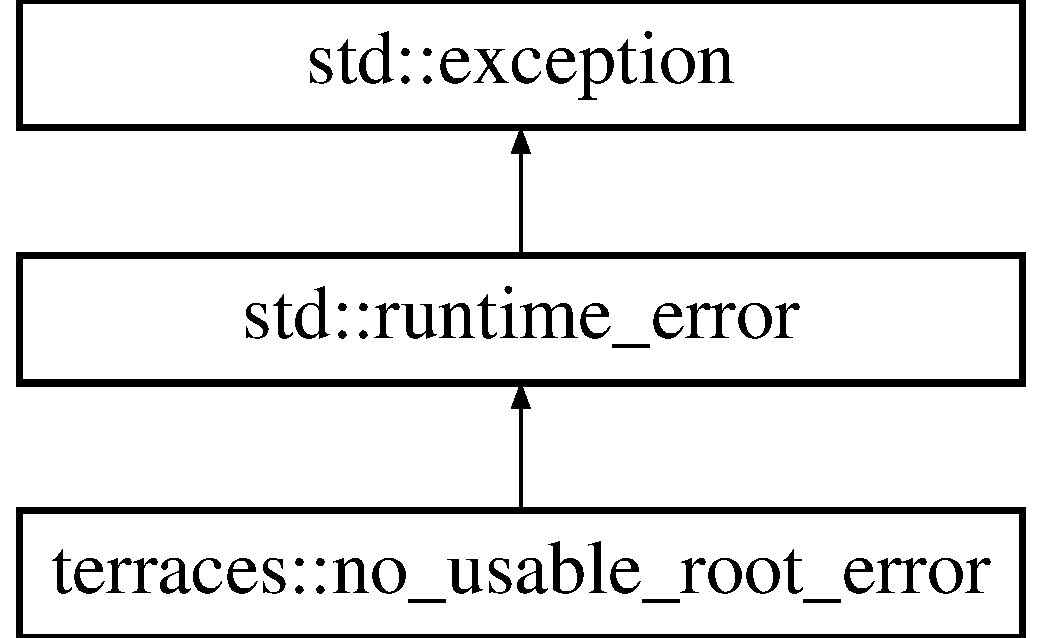
\includegraphics[height=3.000000cm]{classterraces_1_1no__usable__root__error}
\end{center}
\end{figure}


The documentation for this class was generated from the following file\+:\begin{DoxyCompactItemize}
\item 
include/terraces/\hyperlink{errors_8hpp}{errors.\+hpp}\end{DoxyCompactItemize}

\hypertarget{structterraces_1_1node}{}\section{terraces\+:\+:node Struct Reference}
\label{structterraces_1_1node}\index{terraces\+::node@{terraces\+::node}}


{\ttfamily \#include $<$trees.\+hpp$>$}

\subsection*{Public Member Functions}
\begin{DoxyCompactItemize}
\item 
\hyperlink{structterraces_1_1node_aeeaecca04dbbd90b944666d8e1a5c3dc}{node} (\hyperlink{namespaceterraces_adbc33ccb543d1634e96d0eb02e472c77}{index} \hyperlink{structterraces_1_1node_a0dc3c66ea9c5d75867cf529de3d78598}{parent}=none, \hyperlink{namespaceterraces_adbc33ccb543d1634e96d0eb02e472c77}{index} left=none, \hyperlink{namespaceterraces_adbc33ccb543d1634e96d0eb02e472c77}{index} right=none)
\item 
\hyperlink{namespaceterraces_adbc33ccb543d1634e96d0eb02e472c77}{index} \hyperlink{structterraces_1_1node_a0dc3c66ea9c5d75867cf529de3d78598}{parent} () const
\item 
\hyperlink{namespaceterraces_adbc33ccb543d1634e96d0eb02e472c77}{index} \& \hyperlink{structterraces_1_1node_a702158876a59ff469fa1e1fd5a5bca45}{parent} ()
\item 
\hyperlink{namespaceterraces_adbc33ccb543d1634e96d0eb02e472c77}{index} \hyperlink{structterraces_1_1node_a934dadc0e2108504ac7634300d27c3b0}{lchild} () const
\item 
\hyperlink{namespaceterraces_adbc33ccb543d1634e96d0eb02e472c77}{index} \& \hyperlink{structterraces_1_1node_a4df948704080a44771de4909dd94699a}{lchild} ()
\item 
\hyperlink{namespaceterraces_adbc33ccb543d1634e96d0eb02e472c77}{index} \hyperlink{structterraces_1_1node_ab6022c07498a4b1cb9e737fa0ffe4278}{rchild} () const
\item 
\hyperlink{namespaceterraces_adbc33ccb543d1634e96d0eb02e472c77}{index} \& \hyperlink{structterraces_1_1node_a7d53d6f802bc0fa727c67a72033c15ad}{rchild} ()
\item 
bool \hyperlink{structterraces_1_1node_ad0776c1f5b296a8cf52925b4e497814a}{operator==} (const \hyperlink{structterraces_1_1node}{node} \&o) const
\item 
bool \hyperlink{structterraces_1_1node_aebef4e5aff81c490f0fa4ee5ef146484}{operator!=} (const \hyperlink{structterraces_1_1node}{node} \&o) const
\end{DoxyCompactItemize}
\subsection*{Public Attributes}
\begin{DoxyCompactItemize}
\item 
std\+::array$<$ \hyperlink{namespaceterraces_adbc33ccb543d1634e96d0eb02e472c77}{index}, 3 $>$ \hyperlink{structterraces_1_1node_aee217f5c4b1af9fc69f59b278f656663}{data} = \{\{none, none, none\}\}
\end{DoxyCompactItemize}


\subsection{Constructor \& Destructor Documentation}
\mbox{\Hypertarget{structterraces_1_1node_aeeaecca04dbbd90b944666d8e1a5c3dc}\label{structterraces_1_1node_aeeaecca04dbbd90b944666d8e1a5c3dc}} 
\index{terraces\+::node@{terraces\+::node}!node@{node}}
\index{node@{node}!terraces\+::node@{terraces\+::node}}
\subsubsection{\texorpdfstring{node()}{node()}}
{\footnotesize\ttfamily terraces\+::node\+::node (\begin{DoxyParamCaption}\item[{\hyperlink{namespaceterraces_adbc33ccb543d1634e96d0eb02e472c77}{index}}]{parent = {\ttfamily none},  }\item[{\hyperlink{namespaceterraces_adbc33ccb543d1634e96d0eb02e472c77}{index}}]{left = {\ttfamily none},  }\item[{\hyperlink{namespaceterraces_adbc33ccb543d1634e96d0eb02e472c77}{index}}]{right = {\ttfamily none} }\end{DoxyParamCaption})\hspace{0.3cm}{\ttfamily [inline]}}



\subsection{Member Function Documentation}
\mbox{\Hypertarget{structterraces_1_1node_a934dadc0e2108504ac7634300d27c3b0}\label{structterraces_1_1node_a934dadc0e2108504ac7634300d27c3b0}} 
\index{terraces\+::node@{terraces\+::node}!lchild@{lchild}}
\index{lchild@{lchild}!terraces\+::node@{terraces\+::node}}
\subsubsection{\texorpdfstring{lchild()}{lchild()}\hspace{0.1cm}{\footnotesize\ttfamily [1/2]}}
{\footnotesize\ttfamily \hyperlink{namespaceterraces_adbc33ccb543d1634e96d0eb02e472c77}{index} terraces\+::node\+::lchild (\begin{DoxyParamCaption}{ }\end{DoxyParamCaption}) const\hspace{0.3cm}{\ttfamily [inline]}}

\mbox{\Hypertarget{structterraces_1_1node_a4df948704080a44771de4909dd94699a}\label{structterraces_1_1node_a4df948704080a44771de4909dd94699a}} 
\index{terraces\+::node@{terraces\+::node}!lchild@{lchild}}
\index{lchild@{lchild}!terraces\+::node@{terraces\+::node}}
\subsubsection{\texorpdfstring{lchild()}{lchild()}\hspace{0.1cm}{\footnotesize\ttfamily [2/2]}}
{\footnotesize\ttfamily \hyperlink{namespaceterraces_adbc33ccb543d1634e96d0eb02e472c77}{index}\& terraces\+::node\+::lchild (\begin{DoxyParamCaption}{ }\end{DoxyParamCaption})\hspace{0.3cm}{\ttfamily [inline]}}

\mbox{\Hypertarget{structterraces_1_1node_aebef4e5aff81c490f0fa4ee5ef146484}\label{structterraces_1_1node_aebef4e5aff81c490f0fa4ee5ef146484}} 
\index{terraces\+::node@{terraces\+::node}!operator"!=@{operator"!=}}
\index{operator"!=@{operator"!=}!terraces\+::node@{terraces\+::node}}
\subsubsection{\texorpdfstring{operator"!=()}{operator!=()}}
{\footnotesize\ttfamily bool terraces\+::node\+::operator!= (\begin{DoxyParamCaption}\item[{const \hyperlink{structterraces_1_1node}{node} \&}]{o }\end{DoxyParamCaption}) const\hspace{0.3cm}{\ttfamily [inline]}}

\mbox{\Hypertarget{structterraces_1_1node_ad0776c1f5b296a8cf52925b4e497814a}\label{structterraces_1_1node_ad0776c1f5b296a8cf52925b4e497814a}} 
\index{terraces\+::node@{terraces\+::node}!operator==@{operator==}}
\index{operator==@{operator==}!terraces\+::node@{terraces\+::node}}
\subsubsection{\texorpdfstring{operator==()}{operator==()}}
{\footnotesize\ttfamily bool terraces\+::node\+::operator== (\begin{DoxyParamCaption}\item[{const \hyperlink{structterraces_1_1node}{node} \&}]{o }\end{DoxyParamCaption}) const\hspace{0.3cm}{\ttfamily [inline]}}

\mbox{\Hypertarget{structterraces_1_1node_a0dc3c66ea9c5d75867cf529de3d78598}\label{structterraces_1_1node_a0dc3c66ea9c5d75867cf529de3d78598}} 
\index{terraces\+::node@{terraces\+::node}!parent@{parent}}
\index{parent@{parent}!terraces\+::node@{terraces\+::node}}
\subsubsection{\texorpdfstring{parent()}{parent()}\hspace{0.1cm}{\footnotesize\ttfamily [1/2]}}
{\footnotesize\ttfamily \hyperlink{namespaceterraces_adbc33ccb543d1634e96d0eb02e472c77}{index} terraces\+::node\+::parent (\begin{DoxyParamCaption}{ }\end{DoxyParamCaption}) const\hspace{0.3cm}{\ttfamily [inline]}}

\mbox{\Hypertarget{structterraces_1_1node_a702158876a59ff469fa1e1fd5a5bca45}\label{structterraces_1_1node_a702158876a59ff469fa1e1fd5a5bca45}} 
\index{terraces\+::node@{terraces\+::node}!parent@{parent}}
\index{parent@{parent}!terraces\+::node@{terraces\+::node}}
\subsubsection{\texorpdfstring{parent()}{parent()}\hspace{0.1cm}{\footnotesize\ttfamily [2/2]}}
{\footnotesize\ttfamily \hyperlink{namespaceterraces_adbc33ccb543d1634e96d0eb02e472c77}{index}\& terraces\+::node\+::parent (\begin{DoxyParamCaption}{ }\end{DoxyParamCaption})\hspace{0.3cm}{\ttfamily [inline]}}

\mbox{\Hypertarget{structterraces_1_1node_ab6022c07498a4b1cb9e737fa0ffe4278}\label{structterraces_1_1node_ab6022c07498a4b1cb9e737fa0ffe4278}} 
\index{terraces\+::node@{terraces\+::node}!rchild@{rchild}}
\index{rchild@{rchild}!terraces\+::node@{terraces\+::node}}
\subsubsection{\texorpdfstring{rchild()}{rchild()}\hspace{0.1cm}{\footnotesize\ttfamily [1/2]}}
{\footnotesize\ttfamily \hyperlink{namespaceterraces_adbc33ccb543d1634e96d0eb02e472c77}{index} terraces\+::node\+::rchild (\begin{DoxyParamCaption}{ }\end{DoxyParamCaption}) const\hspace{0.3cm}{\ttfamily [inline]}}

\mbox{\Hypertarget{structterraces_1_1node_a7d53d6f802bc0fa727c67a72033c15ad}\label{structterraces_1_1node_a7d53d6f802bc0fa727c67a72033c15ad}} 
\index{terraces\+::node@{terraces\+::node}!rchild@{rchild}}
\index{rchild@{rchild}!terraces\+::node@{terraces\+::node}}
\subsubsection{\texorpdfstring{rchild()}{rchild()}\hspace{0.1cm}{\footnotesize\ttfamily [2/2]}}
{\footnotesize\ttfamily \hyperlink{namespaceterraces_adbc33ccb543d1634e96d0eb02e472c77}{index}\& terraces\+::node\+::rchild (\begin{DoxyParamCaption}{ }\end{DoxyParamCaption})\hspace{0.3cm}{\ttfamily [inline]}}



\subsection{Member Data Documentation}
\mbox{\Hypertarget{structterraces_1_1node_aee217f5c4b1af9fc69f59b278f656663}\label{structterraces_1_1node_aee217f5c4b1af9fc69f59b278f656663}} 
\index{terraces\+::node@{terraces\+::node}!data@{data}}
\index{data@{data}!terraces\+::node@{terraces\+::node}}
\subsubsection{\texorpdfstring{data}{data}}
{\footnotesize\ttfamily std\+::array$<$\hyperlink{namespaceterraces_adbc33ccb543d1634e96d0eb02e472c77}{index}, 3$>$ terraces\+::node\+::data = \{\{none, none, none\}\}}



The documentation for this struct was generated from the following file\+:\begin{DoxyCompactItemize}
\item 
include/terraces/\hyperlink{trees_8hpp}{trees.\+hpp}\end{DoxyCompactItemize}

\hypertarget{structterraces_1_1parsing_1_1parser__state}{}\section{terraces\+:\+:parsing\+:\+:parser\+\_\+state Struct Reference}
\label{structterraces_1_1parsing_1_1parser__state}\index{terraces\+::parsing\+::parser\+\_\+state@{terraces\+::parsing\+::parser\+\_\+state}}
\subsection*{Public Member Functions}
\begin{DoxyCompactItemize}
\item 
\hyperlink{structterraces_1_1parsing_1_1parser__state_a6da424cef05b8f33368f4af9bb7c1734}{parser\+\_\+state} (\hyperlink{namespaceterraces_adbc33ccb543d1634e96d0eb02e472c77}{index} \hyperlink{structterraces_1_1parsing_1_1parser__state_a3cae4795f4aa78de14cfaf743d24d12e}{parent}, \hyperlink{namespaceterraces_adbc33ccb543d1634e96d0eb02e472c77}{index} \hyperlink{structterraces_1_1parsing_1_1parser__state_a4312748dd4f312d8f3022f485866c69c}{self})
\end{DoxyCompactItemize}
\subsection*{Public Attributes}
\begin{DoxyCompactItemize}
\item 
\hyperlink{namespaceterraces_adbc33ccb543d1634e96d0eb02e472c77}{index} \hyperlink{structterraces_1_1parsing_1_1parser__state_a3cae4795f4aa78de14cfaf743d24d12e}{parent}
\item 
\hyperlink{namespaceterraces_adbc33ccb543d1634e96d0eb02e472c77}{index} \hyperlink{structterraces_1_1parsing_1_1parser__state_a4312748dd4f312d8f3022f485866c69c}{self}
\end{DoxyCompactItemize}


\subsection{Constructor \& Destructor Documentation}
\mbox{\Hypertarget{structterraces_1_1parsing_1_1parser__state_a6da424cef05b8f33368f4af9bb7c1734}\label{structterraces_1_1parsing_1_1parser__state_a6da424cef05b8f33368f4af9bb7c1734}} 
\index{terraces\+::parsing\+::parser\+\_\+state@{terraces\+::parsing\+::parser\+\_\+state}!parser\+\_\+state@{parser\+\_\+state}}
\index{parser\+\_\+state@{parser\+\_\+state}!terraces\+::parsing\+::parser\+\_\+state@{terraces\+::parsing\+::parser\+\_\+state}}
\subsubsection{\texorpdfstring{parser\+\_\+state()}{parser\_state()}}
{\footnotesize\ttfamily terraces\+::parsing\+::parser\+\_\+state\+::parser\+\_\+state (\begin{DoxyParamCaption}\item[{\hyperlink{namespaceterraces_adbc33ccb543d1634e96d0eb02e472c77}{index}}]{parent,  }\item[{\hyperlink{namespaceterraces_adbc33ccb543d1634e96d0eb02e472c77}{index}}]{self }\end{DoxyParamCaption})\hspace{0.3cm}{\ttfamily [inline]}}



\subsection{Member Data Documentation}
\mbox{\Hypertarget{structterraces_1_1parsing_1_1parser__state_a3cae4795f4aa78de14cfaf743d24d12e}\label{structterraces_1_1parsing_1_1parser__state_a3cae4795f4aa78de14cfaf743d24d12e}} 
\index{terraces\+::parsing\+::parser\+\_\+state@{terraces\+::parsing\+::parser\+\_\+state}!parent@{parent}}
\index{parent@{parent}!terraces\+::parsing\+::parser\+\_\+state@{terraces\+::parsing\+::parser\+\_\+state}}
\subsubsection{\texorpdfstring{parent}{parent}}
{\footnotesize\ttfamily \hyperlink{namespaceterraces_adbc33ccb543d1634e96d0eb02e472c77}{index} terraces\+::parsing\+::parser\+\_\+state\+::parent}

\mbox{\Hypertarget{structterraces_1_1parsing_1_1parser__state_a4312748dd4f312d8f3022f485866c69c}\label{structterraces_1_1parsing_1_1parser__state_a4312748dd4f312d8f3022f485866c69c}} 
\index{terraces\+::parsing\+::parser\+\_\+state@{terraces\+::parsing\+::parser\+\_\+state}!self@{self}}
\index{self@{self}!terraces\+::parsing\+::parser\+\_\+state@{terraces\+::parsing\+::parser\+\_\+state}}
\subsubsection{\texorpdfstring{self}{self}}
{\footnotesize\ttfamily \hyperlink{namespaceterraces_adbc33ccb543d1634e96d0eb02e472c77}{index} terraces\+::parsing\+::parser\+\_\+state\+::self}



The documentation for this struct was generated from the following file\+:\begin{DoxyCompactItemize}
\item 
lib/\hyperlink{lib_2parser_8cpp}{parser.\+cpp}\end{DoxyCompactItemize}

\hypertarget{structterraces_1_1small__bipartition}{}\section{terraces\+:\+:small\+\_\+bipartition Struct Reference}
\label{structterraces_1_1small__bipartition}\index{terraces\+::small\+\_\+bipartition@{terraces\+::small\+\_\+bipartition}}


{\ttfamily \#include $<$unconstrained\+\_\+enumerator.\+hpp$>$}

\subsection*{Public Member Functions}
\begin{DoxyCompactItemize}
\item 
\hyperlink{structterraces_1_1small__bipartition_a0f2922ef65a57bd424b0f8a200d5c2b9}{small\+\_\+bipartition} (\hyperlink{namespaceterraces_adbc33ccb543d1634e96d0eb02e472c77}{index} \hyperlink{structterraces_1_1small__bipartition_ad1e1ffe92be1066adb84d98c6987d6bb}{mask})
\item 
bool \hyperlink{structterraces_1_1small__bipartition_a8d0f599781285ae580c3fd90254698d0}{is\+\_\+valid} () const
\item 
void \hyperlink{structterraces_1_1small__bipartition_ae47c5f647c0e2fb26ea08011772bea9a}{next} ()
\item 
\hyperlink{namespaceterraces_adbc33ccb543d1634e96d0eb02e472c77}{index} \hyperlink{structterraces_1_1small__bipartition_ad1e1ffe92be1066adb84d98c6987d6bb}{mask} () const
\item 
\hyperlink{namespaceterraces_adbc33ccb543d1634e96d0eb02e472c77}{index} \hyperlink{structterraces_1_1small__bipartition_a907f8818601439b4048d43dc4ffb8364}{left\+\_\+mask} () const
\item 
\hyperlink{namespaceterraces_adbc33ccb543d1634e96d0eb02e472c77}{index} \hyperlink{structterraces_1_1small__bipartition_a54fe7cb417f0e1728fb1d4a8b6c22ba5}{right\+\_\+mask} () const
\item 
\hyperlink{namespaceterraces_adbc33ccb543d1634e96d0eb02e472c77}{index} \hyperlink{structterraces_1_1small__bipartition_ac898947c97bac91255e22be00a5f3e45}{leftmost\+\_\+leaf} () const
\item 
\hyperlink{namespaceterraces_adbc33ccb543d1634e96d0eb02e472c77}{index} \hyperlink{structterraces_1_1small__bipartition_a16a2a79ef1b8e4ca9602adc3263aa597}{rightmost\+\_\+leaf} () const
\item 
\hyperlink{namespaceterraces_adbc33ccb543d1634e96d0eb02e472c77}{index} \hyperlink{structterraces_1_1small__bipartition_aab1364ba4e2e755934b006bb0588a5b8}{num\+\_\+leaves} () const
\end{DoxyCompactItemize}
\subsection*{Public Attributes}
\begin{DoxyCompactItemize}
\item 
const \hyperlink{namespaceterraces_adbc33ccb543d1634e96d0eb02e472c77}{index} \hyperlink{structterraces_1_1small__bipartition_a23458569da8f6402a4c2395a9f5e056f}{m\+\_\+mask}
\item 
const \hyperlink{namespaceterraces_adbc33ccb543d1634e96d0eb02e472c77}{index} \hyperlink{structterraces_1_1small__bipartition_a651c1de5e73b81eefef2497427f9c96c}{m\+\_\+end\+\_\+bip}
\item 
\hyperlink{namespaceterraces_adbc33ccb543d1634e96d0eb02e472c77}{index} \hyperlink{structterraces_1_1small__bipartition_a52eb0315c8109bed2ddfd37d56d77988}{m\+\_\+cur\+\_\+bip}
\end{DoxyCompactItemize}


\subsection{Constructor \& Destructor Documentation}
\mbox{\Hypertarget{structterraces_1_1small__bipartition_a0f2922ef65a57bd424b0f8a200d5c2b9}\label{structterraces_1_1small__bipartition_a0f2922ef65a57bd424b0f8a200d5c2b9}} 
\index{terraces\+::small\+\_\+bipartition@{terraces\+::small\+\_\+bipartition}!small\+\_\+bipartition@{small\+\_\+bipartition}}
\index{small\+\_\+bipartition@{small\+\_\+bipartition}!terraces\+::small\+\_\+bipartition@{terraces\+::small\+\_\+bipartition}}
\subsubsection{\texorpdfstring{small\+\_\+bipartition()}{small\_bipartition()}}
{\footnotesize\ttfamily terraces\+::small\+\_\+bipartition\+::small\+\_\+bipartition (\begin{DoxyParamCaption}\item[{\hyperlink{namespaceterraces_adbc33ccb543d1634e96d0eb02e472c77}{index}}]{mask }\end{DoxyParamCaption})\hspace{0.3cm}{\ttfamily [inline]}}



\subsection{Member Function Documentation}
\mbox{\Hypertarget{structterraces_1_1small__bipartition_a8d0f599781285ae580c3fd90254698d0}\label{structterraces_1_1small__bipartition_a8d0f599781285ae580c3fd90254698d0}} 
\index{terraces\+::small\+\_\+bipartition@{terraces\+::small\+\_\+bipartition}!is\+\_\+valid@{is\+\_\+valid}}
\index{is\+\_\+valid@{is\+\_\+valid}!terraces\+::small\+\_\+bipartition@{terraces\+::small\+\_\+bipartition}}
\subsubsection{\texorpdfstring{is\+\_\+valid()}{is\_valid()}}
{\footnotesize\ttfamily bool terraces\+::small\+\_\+bipartition\+::is\+\_\+valid (\begin{DoxyParamCaption}{ }\end{DoxyParamCaption}) const\hspace{0.3cm}{\ttfamily [inline]}}

\mbox{\Hypertarget{structterraces_1_1small__bipartition_a907f8818601439b4048d43dc4ffb8364}\label{structterraces_1_1small__bipartition_a907f8818601439b4048d43dc4ffb8364}} 
\index{terraces\+::small\+\_\+bipartition@{terraces\+::small\+\_\+bipartition}!left\+\_\+mask@{left\+\_\+mask}}
\index{left\+\_\+mask@{left\+\_\+mask}!terraces\+::small\+\_\+bipartition@{terraces\+::small\+\_\+bipartition}}
\subsubsection{\texorpdfstring{left\+\_\+mask()}{left\_mask()}}
{\footnotesize\ttfamily \hyperlink{namespaceterraces_adbc33ccb543d1634e96d0eb02e472c77}{index} terraces\+::small\+\_\+bipartition\+::left\+\_\+mask (\begin{DoxyParamCaption}{ }\end{DoxyParamCaption}) const\hspace{0.3cm}{\ttfamily [inline]}}

\mbox{\Hypertarget{structterraces_1_1small__bipartition_ac898947c97bac91255e22be00a5f3e45}\label{structterraces_1_1small__bipartition_ac898947c97bac91255e22be00a5f3e45}} 
\index{terraces\+::small\+\_\+bipartition@{terraces\+::small\+\_\+bipartition}!leftmost\+\_\+leaf@{leftmost\+\_\+leaf}}
\index{leftmost\+\_\+leaf@{leftmost\+\_\+leaf}!terraces\+::small\+\_\+bipartition@{terraces\+::small\+\_\+bipartition}}
\subsubsection{\texorpdfstring{leftmost\+\_\+leaf()}{leftmost\_leaf()}}
{\footnotesize\ttfamily \hyperlink{namespaceterraces_adbc33ccb543d1634e96d0eb02e472c77}{index} terraces\+::small\+\_\+bipartition\+::leftmost\+\_\+leaf (\begin{DoxyParamCaption}{ }\end{DoxyParamCaption}) const\hspace{0.3cm}{\ttfamily [inline]}}

\mbox{\Hypertarget{structterraces_1_1small__bipartition_ad1e1ffe92be1066adb84d98c6987d6bb}\label{structterraces_1_1small__bipartition_ad1e1ffe92be1066adb84d98c6987d6bb}} 
\index{terraces\+::small\+\_\+bipartition@{terraces\+::small\+\_\+bipartition}!mask@{mask}}
\index{mask@{mask}!terraces\+::small\+\_\+bipartition@{terraces\+::small\+\_\+bipartition}}
\subsubsection{\texorpdfstring{mask()}{mask()}}
{\footnotesize\ttfamily \hyperlink{namespaceterraces_adbc33ccb543d1634e96d0eb02e472c77}{index} terraces\+::small\+\_\+bipartition\+::mask (\begin{DoxyParamCaption}{ }\end{DoxyParamCaption}) const\hspace{0.3cm}{\ttfamily [inline]}}

\mbox{\Hypertarget{structterraces_1_1small__bipartition_ae47c5f647c0e2fb26ea08011772bea9a}\label{structterraces_1_1small__bipartition_ae47c5f647c0e2fb26ea08011772bea9a}} 
\index{terraces\+::small\+\_\+bipartition@{terraces\+::small\+\_\+bipartition}!next@{next}}
\index{next@{next}!terraces\+::small\+\_\+bipartition@{terraces\+::small\+\_\+bipartition}}
\subsubsection{\texorpdfstring{next()}{next()}}
{\footnotesize\ttfamily void terraces\+::small\+\_\+bipartition\+::next (\begin{DoxyParamCaption}{ }\end{DoxyParamCaption})\hspace{0.3cm}{\ttfamily [inline]}}

\mbox{\Hypertarget{structterraces_1_1small__bipartition_aab1364ba4e2e755934b006bb0588a5b8}\label{structterraces_1_1small__bipartition_aab1364ba4e2e755934b006bb0588a5b8}} 
\index{terraces\+::small\+\_\+bipartition@{terraces\+::small\+\_\+bipartition}!num\+\_\+leaves@{num\+\_\+leaves}}
\index{num\+\_\+leaves@{num\+\_\+leaves}!terraces\+::small\+\_\+bipartition@{terraces\+::small\+\_\+bipartition}}
\subsubsection{\texorpdfstring{num\+\_\+leaves()}{num\_leaves()}}
{\footnotesize\ttfamily \hyperlink{namespaceterraces_adbc33ccb543d1634e96d0eb02e472c77}{index} terraces\+::small\+\_\+bipartition\+::num\+\_\+leaves (\begin{DoxyParamCaption}{ }\end{DoxyParamCaption}) const\hspace{0.3cm}{\ttfamily [inline]}}

\mbox{\Hypertarget{structterraces_1_1small__bipartition_a54fe7cb417f0e1728fb1d4a8b6c22ba5}\label{structterraces_1_1small__bipartition_a54fe7cb417f0e1728fb1d4a8b6c22ba5}} 
\index{terraces\+::small\+\_\+bipartition@{terraces\+::small\+\_\+bipartition}!right\+\_\+mask@{right\+\_\+mask}}
\index{right\+\_\+mask@{right\+\_\+mask}!terraces\+::small\+\_\+bipartition@{terraces\+::small\+\_\+bipartition}}
\subsubsection{\texorpdfstring{right\+\_\+mask()}{right\_mask()}}
{\footnotesize\ttfamily \hyperlink{namespaceterraces_adbc33ccb543d1634e96d0eb02e472c77}{index} terraces\+::small\+\_\+bipartition\+::right\+\_\+mask (\begin{DoxyParamCaption}{ }\end{DoxyParamCaption}) const\hspace{0.3cm}{\ttfamily [inline]}}

\mbox{\Hypertarget{structterraces_1_1small__bipartition_a16a2a79ef1b8e4ca9602adc3263aa597}\label{structterraces_1_1small__bipartition_a16a2a79ef1b8e4ca9602adc3263aa597}} 
\index{terraces\+::small\+\_\+bipartition@{terraces\+::small\+\_\+bipartition}!rightmost\+\_\+leaf@{rightmost\+\_\+leaf}}
\index{rightmost\+\_\+leaf@{rightmost\+\_\+leaf}!terraces\+::small\+\_\+bipartition@{terraces\+::small\+\_\+bipartition}}
\subsubsection{\texorpdfstring{rightmost\+\_\+leaf()}{rightmost\_leaf()}}
{\footnotesize\ttfamily \hyperlink{namespaceterraces_adbc33ccb543d1634e96d0eb02e472c77}{index} terraces\+::small\+\_\+bipartition\+::rightmost\+\_\+leaf (\begin{DoxyParamCaption}{ }\end{DoxyParamCaption}) const\hspace{0.3cm}{\ttfamily [inline]}}



\subsection{Member Data Documentation}
\mbox{\Hypertarget{structterraces_1_1small__bipartition_a52eb0315c8109bed2ddfd37d56d77988}\label{structterraces_1_1small__bipartition_a52eb0315c8109bed2ddfd37d56d77988}} 
\index{terraces\+::small\+\_\+bipartition@{terraces\+::small\+\_\+bipartition}!m\+\_\+cur\+\_\+bip@{m\+\_\+cur\+\_\+bip}}
\index{m\+\_\+cur\+\_\+bip@{m\+\_\+cur\+\_\+bip}!terraces\+::small\+\_\+bipartition@{terraces\+::small\+\_\+bipartition}}
\subsubsection{\texorpdfstring{m\+\_\+cur\+\_\+bip}{m\_cur\_bip}}
{\footnotesize\ttfamily \hyperlink{namespaceterraces_adbc33ccb543d1634e96d0eb02e472c77}{index} terraces\+::small\+\_\+bipartition\+::m\+\_\+cur\+\_\+bip}

\mbox{\Hypertarget{structterraces_1_1small__bipartition_a651c1de5e73b81eefef2497427f9c96c}\label{structterraces_1_1small__bipartition_a651c1de5e73b81eefef2497427f9c96c}} 
\index{terraces\+::small\+\_\+bipartition@{terraces\+::small\+\_\+bipartition}!m\+\_\+end\+\_\+bip@{m\+\_\+end\+\_\+bip}}
\index{m\+\_\+end\+\_\+bip@{m\+\_\+end\+\_\+bip}!terraces\+::small\+\_\+bipartition@{terraces\+::small\+\_\+bipartition}}
\subsubsection{\texorpdfstring{m\+\_\+end\+\_\+bip}{m\_end\_bip}}
{\footnotesize\ttfamily const \hyperlink{namespaceterraces_adbc33ccb543d1634e96d0eb02e472c77}{index} terraces\+::small\+\_\+bipartition\+::m\+\_\+end\+\_\+bip}

\mbox{\Hypertarget{structterraces_1_1small__bipartition_a23458569da8f6402a4c2395a9f5e056f}\label{structterraces_1_1small__bipartition_a23458569da8f6402a4c2395a9f5e056f}} 
\index{terraces\+::small\+\_\+bipartition@{terraces\+::small\+\_\+bipartition}!m\+\_\+mask@{m\+\_\+mask}}
\index{m\+\_\+mask@{m\+\_\+mask}!terraces\+::small\+\_\+bipartition@{terraces\+::small\+\_\+bipartition}}
\subsubsection{\texorpdfstring{m\+\_\+mask}{m\_mask}}
{\footnotesize\ttfamily const \hyperlink{namespaceterraces_adbc33ccb543d1634e96d0eb02e472c77}{index} terraces\+::small\+\_\+bipartition\+::m\+\_\+mask}



The documentation for this struct was generated from the following file\+:\begin{DoxyCompactItemize}
\item 
lib/\hyperlink{unconstrained__enumerator_8hpp}{unconstrained\+\_\+enumerator.\+hpp}\end{DoxyCompactItemize}

\hypertarget{classterraces_1_1utils_1_1stack__allocator}{}\section{terraces\+:\+:utils\+:\+:stack\+\_\+allocator$<$ T $>$ Class Template Reference}
\label{classterraces_1_1utils_1_1stack__allocator}\index{terraces\+::utils\+::stack\+\_\+allocator$<$ T $>$@{terraces\+::utils\+::stack\+\_\+allocator$<$ T $>$}}


{\ttfamily \#include $<$stack\+\_\+allocator.\+hpp$>$}

\subsection*{Public Types}
\begin{DoxyCompactItemize}
\item 
using \hyperlink{classterraces_1_1utils_1_1stack__allocator_a1c3fa04869c7fe9730a18b046461cbbb}{value\+\_\+type} = T
\end{DoxyCompactItemize}
\subsection*{Public Member Functions}
\begin{DoxyCompactItemize}
\item 
\hyperlink{classterraces_1_1utils_1_1stack__allocator_a557138c2f8f21847dbbfbdc588909f68}{stack\+\_\+allocator} (\hyperlink{classterraces_1_1utils_1_1free__list}{free\+\_\+list} \&fl, std\+::size\+\_\+t n)
\item 
{\footnotesize template$<$typename U $>$ }\\\hyperlink{classterraces_1_1utils_1_1stack__allocator_a786655b3258a2c776901389ca5c1c762}{stack\+\_\+allocator} (const \hyperlink{classterraces_1_1utils_1_1stack__allocator}{stack\+\_\+allocator}$<$ U $>$ \&other)
\item 
T $\ast$ \hyperlink{classterraces_1_1utils_1_1stack__allocator_afcc195b71e290468330bf444ab27a237}{allocate} (std\+::size\+\_\+t n)
\item 
void \hyperlink{classterraces_1_1utils_1_1stack__allocator_a804f63d9b9f82e5462dae9a43144ec82}{deallocate} (T $\ast$ptr, std\+::size\+\_\+t)
\end{DoxyCompactItemize}
\subsection*{Friends}
\begin{DoxyCompactItemize}
\item 
{\footnotesize template$<$typename U $>$ }\\class \hyperlink{classterraces_1_1utils_1_1stack__allocator_a63e83703d59c04427b11c879b4f4a637}{stack\+\_\+allocator}
\item 
bool \hyperlink{classterraces_1_1utils_1_1stack__allocator_a4f03647bb7adb25d049daf9e4e741301}{operator==} (const \hyperlink{classterraces_1_1utils_1_1stack__allocator}{stack\+\_\+allocator} \&lhs, const \hyperlink{classterraces_1_1utils_1_1stack__allocator}{stack\+\_\+allocator} \&rhs)
\end{DoxyCompactItemize}


\subsection{Member Typedef Documentation}
\mbox{\Hypertarget{classterraces_1_1utils_1_1stack__allocator_a1c3fa04869c7fe9730a18b046461cbbb}\label{classterraces_1_1utils_1_1stack__allocator_a1c3fa04869c7fe9730a18b046461cbbb}} 
\index{terraces\+::utils\+::stack\+\_\+allocator@{terraces\+::utils\+::stack\+\_\+allocator}!value\+\_\+type@{value\+\_\+type}}
\index{value\+\_\+type@{value\+\_\+type}!terraces\+::utils\+::stack\+\_\+allocator@{terraces\+::utils\+::stack\+\_\+allocator}}
\subsubsection{\texorpdfstring{value\+\_\+type}{value\_type}}
{\footnotesize\ttfamily template$<$typename T$>$ \\
using \hyperlink{classterraces_1_1utils_1_1stack__allocator}{terraces\+::utils\+::stack\+\_\+allocator}$<$ T $>$\+::\hyperlink{classterraces_1_1utils_1_1stack__allocator_a1c3fa04869c7fe9730a18b046461cbbb}{value\+\_\+type} =  T}



\subsection{Constructor \& Destructor Documentation}
\mbox{\Hypertarget{classterraces_1_1utils_1_1stack__allocator_a557138c2f8f21847dbbfbdc588909f68}\label{classterraces_1_1utils_1_1stack__allocator_a557138c2f8f21847dbbfbdc588909f68}} 
\index{terraces\+::utils\+::stack\+\_\+allocator@{terraces\+::utils\+::stack\+\_\+allocator}!stack\+\_\+allocator@{stack\+\_\+allocator}}
\index{stack\+\_\+allocator@{stack\+\_\+allocator}!terraces\+::utils\+::stack\+\_\+allocator@{terraces\+::utils\+::stack\+\_\+allocator}}
\subsubsection{\texorpdfstring{stack\+\_\+allocator()}{stack\_allocator()}\hspace{0.1cm}{\footnotesize\ttfamily [1/2]}}
{\footnotesize\ttfamily template$<$typename T$>$ \\
\hyperlink{classterraces_1_1utils_1_1stack__allocator}{terraces\+::utils\+::stack\+\_\+allocator}$<$ T $>$\+::\hyperlink{classterraces_1_1utils_1_1stack__allocator}{stack\+\_\+allocator} (\begin{DoxyParamCaption}\item[{\hyperlink{classterraces_1_1utils_1_1free__list}{free\+\_\+list} \&}]{fl,  }\item[{std\+::size\+\_\+t}]{n }\end{DoxyParamCaption})\hspace{0.3cm}{\ttfamily [inline]}}

\mbox{\Hypertarget{classterraces_1_1utils_1_1stack__allocator_a786655b3258a2c776901389ca5c1c762}\label{classterraces_1_1utils_1_1stack__allocator_a786655b3258a2c776901389ca5c1c762}} 
\index{terraces\+::utils\+::stack\+\_\+allocator@{terraces\+::utils\+::stack\+\_\+allocator}!stack\+\_\+allocator@{stack\+\_\+allocator}}
\index{stack\+\_\+allocator@{stack\+\_\+allocator}!terraces\+::utils\+::stack\+\_\+allocator@{terraces\+::utils\+::stack\+\_\+allocator}}
\subsubsection{\texorpdfstring{stack\+\_\+allocator()}{stack\_allocator()}\hspace{0.1cm}{\footnotesize\ttfamily [2/2]}}
{\footnotesize\ttfamily template$<$typename T$>$ \\
template$<$typename U $>$ \\
\hyperlink{classterraces_1_1utils_1_1stack__allocator}{terraces\+::utils\+::stack\+\_\+allocator}$<$ T $>$\+::\hyperlink{classterraces_1_1utils_1_1stack__allocator}{stack\+\_\+allocator} (\begin{DoxyParamCaption}\item[{const \hyperlink{classterraces_1_1utils_1_1stack__allocator}{stack\+\_\+allocator}$<$ U $>$ \&}]{other }\end{DoxyParamCaption})\hspace{0.3cm}{\ttfamily [inline]}}



\subsection{Member Function Documentation}
\mbox{\Hypertarget{classterraces_1_1utils_1_1stack__allocator_afcc195b71e290468330bf444ab27a237}\label{classterraces_1_1utils_1_1stack__allocator_afcc195b71e290468330bf444ab27a237}} 
\index{terraces\+::utils\+::stack\+\_\+allocator@{terraces\+::utils\+::stack\+\_\+allocator}!allocate@{allocate}}
\index{allocate@{allocate}!terraces\+::utils\+::stack\+\_\+allocator@{terraces\+::utils\+::stack\+\_\+allocator}}
\subsubsection{\texorpdfstring{allocate()}{allocate()}}
{\footnotesize\ttfamily template$<$typename T$>$ \\
T$\ast$ \hyperlink{classterraces_1_1utils_1_1stack__allocator}{terraces\+::utils\+::stack\+\_\+allocator}$<$ T $>$\+::allocate (\begin{DoxyParamCaption}\item[{std\+::size\+\_\+t}]{n }\end{DoxyParamCaption})\hspace{0.3cm}{\ttfamily [inline]}}

\mbox{\Hypertarget{classterraces_1_1utils_1_1stack__allocator_a804f63d9b9f82e5462dae9a43144ec82}\label{classterraces_1_1utils_1_1stack__allocator_a804f63d9b9f82e5462dae9a43144ec82}} 
\index{terraces\+::utils\+::stack\+\_\+allocator@{terraces\+::utils\+::stack\+\_\+allocator}!deallocate@{deallocate}}
\index{deallocate@{deallocate}!terraces\+::utils\+::stack\+\_\+allocator@{terraces\+::utils\+::stack\+\_\+allocator}}
\subsubsection{\texorpdfstring{deallocate()}{deallocate()}}
{\footnotesize\ttfamily template$<$typename T$>$ \\
void \hyperlink{classterraces_1_1utils_1_1stack__allocator}{terraces\+::utils\+::stack\+\_\+allocator}$<$ T $>$\+::deallocate (\begin{DoxyParamCaption}\item[{T $\ast$}]{ptr,  }\item[{std\+::size\+\_\+t}]{ }\end{DoxyParamCaption})\hspace{0.3cm}{\ttfamily [inline]}}



\subsection{Friends And Related Function Documentation}
\mbox{\Hypertarget{classterraces_1_1utils_1_1stack__allocator_a4f03647bb7adb25d049daf9e4e741301}\label{classterraces_1_1utils_1_1stack__allocator_a4f03647bb7adb25d049daf9e4e741301}} 
\index{terraces\+::utils\+::stack\+\_\+allocator@{terraces\+::utils\+::stack\+\_\+allocator}!operator==@{operator==}}
\index{operator==@{operator==}!terraces\+::utils\+::stack\+\_\+allocator@{terraces\+::utils\+::stack\+\_\+allocator}}
\subsubsection{\texorpdfstring{operator==}{operator==}}
{\footnotesize\ttfamily template$<$typename T$>$ \\
bool operator== (\begin{DoxyParamCaption}\item[{const \hyperlink{classterraces_1_1utils_1_1stack__allocator}{stack\+\_\+allocator}$<$ T $>$ \&}]{lhs,  }\item[{const \hyperlink{classterraces_1_1utils_1_1stack__allocator}{stack\+\_\+allocator}$<$ T $>$ \&}]{rhs }\end{DoxyParamCaption})\hspace{0.3cm}{\ttfamily [friend]}}

\mbox{\Hypertarget{classterraces_1_1utils_1_1stack__allocator_a63e83703d59c04427b11c879b4f4a637}\label{classterraces_1_1utils_1_1stack__allocator_a63e83703d59c04427b11c879b4f4a637}} 
\index{terraces\+::utils\+::stack\+\_\+allocator@{terraces\+::utils\+::stack\+\_\+allocator}!stack\+\_\+allocator@{stack\+\_\+allocator}}
\index{stack\+\_\+allocator@{stack\+\_\+allocator}!terraces\+::utils\+::stack\+\_\+allocator@{terraces\+::utils\+::stack\+\_\+allocator}}
\subsubsection{\texorpdfstring{stack\+\_\+allocator}{stack\_allocator}}
{\footnotesize\ttfamily template$<$typename T$>$ \\
template$<$typename U $>$ \\
friend class \hyperlink{classterraces_1_1utils_1_1stack__allocator}{stack\+\_\+allocator}\hspace{0.3cm}{\ttfamily [friend]}}



The documentation for this class was generated from the following file\+:\begin{DoxyCompactItemize}
\item 
lib/\hyperlink{stack__allocator_8hpp}{stack\+\_\+allocator.\+hpp}\end{DoxyCompactItemize}

\hypertarget{structterraces_1_1debug_1_1variants_1_1stack__state}{}\section{terraces\+:\+:debug\+:\+:variants\+:\+:stack\+\_\+state$<$ Result $>$ Struct Template Reference}
\label{structterraces_1_1debug_1_1variants_1_1stack__state}\index{terraces\+::debug\+::variants\+::stack\+\_\+state$<$ Result $>$@{terraces\+::debug\+::variants\+::stack\+\_\+state$<$ Result $>$}}


{\ttfamily \#include $<$supertree\+\_\+variants\+\_\+debug.\+hpp$>$}

\subsection*{Public Member Functions}
\begin{DoxyCompactItemize}
\item 
\hyperlink{structterraces_1_1debug_1_1variants_1_1stack__state_aa6e7dd897252ad8b00833ba51f488ef1}{stack\+\_\+state} (Result \hyperlink{structterraces_1_1debug_1_1variants_1_1stack__state_a808ad42bf719be610fb8b85c426858a1}{intermediate})
\end{DoxyCompactItemize}
\subsection*{Public Attributes}
\begin{DoxyCompactItemize}
\item 
\hyperlink{namespaceterraces_adbc33ccb543d1634e96d0eb02e472c77}{index} \hyperlink{structterraces_1_1debug_1_1variants_1_1stack__state_a99c9586ee3fc9e182d85d5c9bec85175}{current\+\_\+bip}
\item 
\hyperlink{namespaceterraces_adbc33ccb543d1634e96d0eb02e472c77}{index} \hyperlink{structterraces_1_1debug_1_1variants_1_1stack__state_aed75425f1d76ae6bec3e9a733bf8de9d}{max\+\_\+bip}
\item 
bool \hyperlink{structterraces_1_1debug_1_1variants_1_1stack__state_a3b6c53beae52fe9d9afce640c6ea08e4}{right}
\item 
Result \hyperlink{structterraces_1_1debug_1_1variants_1_1stack__state_a808ad42bf719be610fb8b85c426858a1}{intermediate}
\end{DoxyCompactItemize}


\subsection{Constructor \& Destructor Documentation}
\mbox{\Hypertarget{structterraces_1_1debug_1_1variants_1_1stack__state_aa6e7dd897252ad8b00833ba51f488ef1}\label{structterraces_1_1debug_1_1variants_1_1stack__state_aa6e7dd897252ad8b00833ba51f488ef1}} 
\index{terraces\+::debug\+::variants\+::stack\+\_\+state@{terraces\+::debug\+::variants\+::stack\+\_\+state}!stack\+\_\+state@{stack\+\_\+state}}
\index{stack\+\_\+state@{stack\+\_\+state}!terraces\+::debug\+::variants\+::stack\+\_\+state@{terraces\+::debug\+::variants\+::stack\+\_\+state}}
\subsubsection{\texorpdfstring{stack\+\_\+state()}{stack\_state()}}
{\footnotesize\ttfamily template$<$typename Result$>$ \\
\hyperlink{structterraces_1_1debug_1_1variants_1_1stack__state}{terraces\+::debug\+::variants\+::stack\+\_\+state}$<$ Result $>$\+::\hyperlink{structterraces_1_1debug_1_1variants_1_1stack__state}{stack\+\_\+state} (\begin{DoxyParamCaption}\item[{Result}]{intermediate }\end{DoxyParamCaption})\hspace{0.3cm}{\ttfamily [inline]}}



\subsection{Member Data Documentation}
\mbox{\Hypertarget{structterraces_1_1debug_1_1variants_1_1stack__state_a99c9586ee3fc9e182d85d5c9bec85175}\label{structterraces_1_1debug_1_1variants_1_1stack__state_a99c9586ee3fc9e182d85d5c9bec85175}} 
\index{terraces\+::debug\+::variants\+::stack\+\_\+state@{terraces\+::debug\+::variants\+::stack\+\_\+state}!current\+\_\+bip@{current\+\_\+bip}}
\index{current\+\_\+bip@{current\+\_\+bip}!terraces\+::debug\+::variants\+::stack\+\_\+state@{terraces\+::debug\+::variants\+::stack\+\_\+state}}
\subsubsection{\texorpdfstring{current\+\_\+bip}{current\_bip}}
{\footnotesize\ttfamily template$<$typename Result$>$ \\
\hyperlink{namespaceterraces_adbc33ccb543d1634e96d0eb02e472c77}{index} \hyperlink{structterraces_1_1debug_1_1variants_1_1stack__state}{terraces\+::debug\+::variants\+::stack\+\_\+state}$<$ Result $>$\+::current\+\_\+bip}

\mbox{\Hypertarget{structterraces_1_1debug_1_1variants_1_1stack__state_a808ad42bf719be610fb8b85c426858a1}\label{structterraces_1_1debug_1_1variants_1_1stack__state_a808ad42bf719be610fb8b85c426858a1}} 
\index{terraces\+::debug\+::variants\+::stack\+\_\+state@{terraces\+::debug\+::variants\+::stack\+\_\+state}!intermediate@{intermediate}}
\index{intermediate@{intermediate}!terraces\+::debug\+::variants\+::stack\+\_\+state@{terraces\+::debug\+::variants\+::stack\+\_\+state}}
\subsubsection{\texorpdfstring{intermediate}{intermediate}}
{\footnotesize\ttfamily template$<$typename Result$>$ \\
Result \hyperlink{structterraces_1_1debug_1_1variants_1_1stack__state}{terraces\+::debug\+::variants\+::stack\+\_\+state}$<$ Result $>$\+::intermediate}

\mbox{\Hypertarget{structterraces_1_1debug_1_1variants_1_1stack__state_aed75425f1d76ae6bec3e9a733bf8de9d}\label{structterraces_1_1debug_1_1variants_1_1stack__state_aed75425f1d76ae6bec3e9a733bf8de9d}} 
\index{terraces\+::debug\+::variants\+::stack\+\_\+state@{terraces\+::debug\+::variants\+::stack\+\_\+state}!max\+\_\+bip@{max\+\_\+bip}}
\index{max\+\_\+bip@{max\+\_\+bip}!terraces\+::debug\+::variants\+::stack\+\_\+state@{terraces\+::debug\+::variants\+::stack\+\_\+state}}
\subsubsection{\texorpdfstring{max\+\_\+bip}{max\_bip}}
{\footnotesize\ttfamily template$<$typename Result$>$ \\
\hyperlink{namespaceterraces_adbc33ccb543d1634e96d0eb02e472c77}{index} \hyperlink{structterraces_1_1debug_1_1variants_1_1stack__state}{terraces\+::debug\+::variants\+::stack\+\_\+state}$<$ Result $>$\+::max\+\_\+bip}

\mbox{\Hypertarget{structterraces_1_1debug_1_1variants_1_1stack__state_a3b6c53beae52fe9d9afce640c6ea08e4}\label{structterraces_1_1debug_1_1variants_1_1stack__state_a3b6c53beae52fe9d9afce640c6ea08e4}} 
\index{terraces\+::debug\+::variants\+::stack\+\_\+state@{terraces\+::debug\+::variants\+::stack\+\_\+state}!right@{right}}
\index{right@{right}!terraces\+::debug\+::variants\+::stack\+\_\+state@{terraces\+::debug\+::variants\+::stack\+\_\+state}}
\subsubsection{\texorpdfstring{right}{right}}
{\footnotesize\ttfamily template$<$typename Result$>$ \\
bool \hyperlink{structterraces_1_1debug_1_1variants_1_1stack__state}{terraces\+::debug\+::variants\+::stack\+\_\+state}$<$ Result $>$\+::right}



The documentation for this struct was generated from the following file\+:\begin{DoxyCompactItemize}
\item 
lib/\hyperlink{supertree__variants__debug_8hpp}{supertree\+\_\+variants\+\_\+debug.\+hpp}\end{DoxyCompactItemize}

\hypertarget{classterraces_1_1debug_1_1variants_1_1stack__state__decorator}{}\section{terraces\+:\+:debug\+:\+:variants\+:\+:stack\+\_\+state\+\_\+decorator$<$ Callback $>$ Class Template Reference}
\label{classterraces_1_1debug_1_1variants_1_1stack__state__decorator}\index{terraces\+::debug\+::variants\+::stack\+\_\+state\+\_\+decorator$<$ Callback $>$@{terraces\+::debug\+::variants\+::stack\+\_\+state\+\_\+decorator$<$ Callback $>$}}


{\ttfamily \#include $<$supertree\+\_\+variants\+\_\+debug.\+hpp$>$}

Inheritance diagram for terraces\+:\+:debug\+:\+:variants\+:\+:stack\+\_\+state\+\_\+decorator$<$ Callback $>$\+:\begin{figure}[H]
\begin{center}
\leavevmode
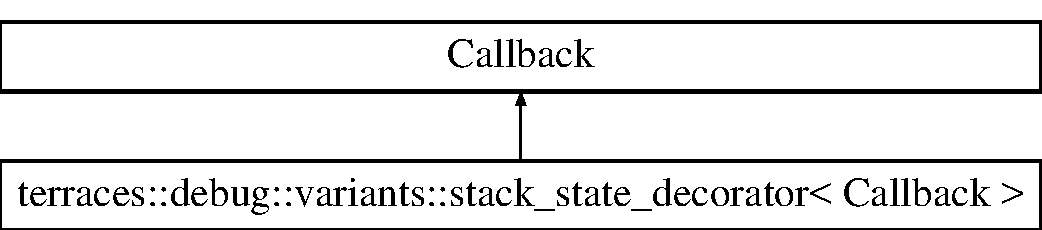
\includegraphics[height=2.000000cm]{classterraces_1_1debug_1_1variants_1_1stack__state__decorator}
\end{center}
\end{figure}
\subsection*{Public Types}
\begin{DoxyCompactItemize}
\item 
using \hyperlink{classterraces_1_1debug_1_1variants_1_1stack__state__decorator_a01062643b31a3124c3e77d409f112785}{result\+\_\+type} = typename Callback\+::result\+\_\+type
\end{DoxyCompactItemize}
\subsection*{Public Member Functions}
\begin{DoxyCompactItemize}
\item 
{\footnotesize template$<$typename... Args$>$ }\\\hyperlink{classterraces_1_1debug_1_1variants_1_1stack__state__decorator_a1f72f35c4ec868bb5bba02806c7ddbb3}{stack\+\_\+state\+\_\+decorator} (Args \&\&... args)
\item 
\hyperlink{classterraces_1_1debug_1_1variants_1_1stack__state__decorator_a01062643b31a3124c3e77d409f112785}{result\+\_\+type} \hyperlink{classterraces_1_1debug_1_1variants_1_1stack__state__decorator_ac650dee955aa719620f14c93ed67820d}{begin\+\_\+iteration} (const \hyperlink{classterraces_1_1bipartition__iterator}{bipartition\+\_\+iterator} \&bip\+\_\+it, const \hyperlink{namespaceterraces_a1b526fb554dff829f7ad51eb21d5ed06}{bitvector} \&c\+\_\+occ, const \hyperlink{namespaceterraces_a6f603ffd30ed4d902fce6424492e0581}{constraints} \&\hyperlink{namespaceterraces_a6f603ffd30ed4d902fce6424492e0581}{constraints})
\item 
void \hyperlink{classterraces_1_1debug_1_1variants_1_1stack__state__decorator_a1f93e11840c3fed2902f925a2fb10f5f}{step\+\_\+iteration} (const \hyperlink{classterraces_1_1bipartition__iterator}{bipartition\+\_\+iterator} \&bip\+\_\+it)
\item 
void \hyperlink{classterraces_1_1debug_1_1variants_1_1stack__state__decorator_ac09a4841c6a5b236ae9bd3ec8bf39b77}{finish\+\_\+iteration} ()
\item 
void \hyperlink{classterraces_1_1debug_1_1variants_1_1stack__state__decorator_a6d1de019820009248a9362a3407c7b94}{right\+\_\+subcall} ()
\item 
void \hyperlink{classterraces_1_1debug_1_1variants_1_1stack__state__decorator_a2dcd5551b46929e3a4a1ddcca619f6e4}{left\+\_\+subcall} ()
\item 
\hyperlink{classterraces_1_1debug_1_1variants_1_1stack__state__decorator_a01062643b31a3124c3e77d409f112785}{result\+\_\+type} \hyperlink{classterraces_1_1debug_1_1variants_1_1stack__state__decorator_a3ab51f3a9522d1ba4b068d00f5d74e0a}{accumulate} (\hyperlink{classterraces_1_1debug_1_1variants_1_1stack__state__decorator_a01062643b31a3124c3e77d409f112785}{result\+\_\+type} acc, \hyperlink{classterraces_1_1debug_1_1variants_1_1stack__state__decorator_a01062643b31a3124c3e77d409f112785}{result\+\_\+type} val)
\item 
const std\+::vector$<$ \hyperlink{structterraces_1_1debug_1_1variants_1_1stack__state}{stack\+\_\+state}$<$ \hyperlink{classterraces_1_1debug_1_1variants_1_1stack__state__decorator_a01062643b31a3124c3e77d409f112785}{result\+\_\+type} $>$ $>$ \& \hyperlink{classterraces_1_1debug_1_1variants_1_1stack__state__decorator_a371be3718c4eb307a46f313db17cfd18}{stack} () const
\end{DoxyCompactItemize}


\subsection{Member Typedef Documentation}
\mbox{\Hypertarget{classterraces_1_1debug_1_1variants_1_1stack__state__decorator_a01062643b31a3124c3e77d409f112785}\label{classterraces_1_1debug_1_1variants_1_1stack__state__decorator_a01062643b31a3124c3e77d409f112785}} 
\index{terraces\+::debug\+::variants\+::stack\+\_\+state\+\_\+decorator@{terraces\+::debug\+::variants\+::stack\+\_\+state\+\_\+decorator}!result\+\_\+type@{result\+\_\+type}}
\index{result\+\_\+type@{result\+\_\+type}!terraces\+::debug\+::variants\+::stack\+\_\+state\+\_\+decorator@{terraces\+::debug\+::variants\+::stack\+\_\+state\+\_\+decorator}}
\subsubsection{\texorpdfstring{result\+\_\+type}{result\_type}}
{\footnotesize\ttfamily template$<$typename Callback $>$ \\
using \hyperlink{classterraces_1_1debug_1_1variants_1_1stack__state__decorator}{terraces\+::debug\+::variants\+::stack\+\_\+state\+\_\+decorator}$<$ Callback $>$\+::\hyperlink{classterraces_1_1debug_1_1variants_1_1stack__state__decorator_a01062643b31a3124c3e77d409f112785}{result\+\_\+type} =  typename Callback\+::result\+\_\+type}



\subsection{Constructor \& Destructor Documentation}
\mbox{\Hypertarget{classterraces_1_1debug_1_1variants_1_1stack__state__decorator_a1f72f35c4ec868bb5bba02806c7ddbb3}\label{classterraces_1_1debug_1_1variants_1_1stack__state__decorator_a1f72f35c4ec868bb5bba02806c7ddbb3}} 
\index{terraces\+::debug\+::variants\+::stack\+\_\+state\+\_\+decorator@{terraces\+::debug\+::variants\+::stack\+\_\+state\+\_\+decorator}!stack\+\_\+state\+\_\+decorator@{stack\+\_\+state\+\_\+decorator}}
\index{stack\+\_\+state\+\_\+decorator@{stack\+\_\+state\+\_\+decorator}!terraces\+::debug\+::variants\+::stack\+\_\+state\+\_\+decorator@{terraces\+::debug\+::variants\+::stack\+\_\+state\+\_\+decorator}}
\subsubsection{\texorpdfstring{stack\+\_\+state\+\_\+decorator()}{stack\_state\_decorator()}}
{\footnotesize\ttfamily template$<$typename Callback $>$ \\
template$<$typename... Args$>$ \\
\hyperlink{classterraces_1_1debug_1_1variants_1_1stack__state__decorator}{terraces\+::debug\+::variants\+::stack\+\_\+state\+\_\+decorator}$<$ Callback $>$\+::\hyperlink{classterraces_1_1debug_1_1variants_1_1stack__state__decorator}{stack\+\_\+state\+\_\+decorator} (\begin{DoxyParamCaption}\item[{Args \&\&...}]{args }\end{DoxyParamCaption})\hspace{0.3cm}{\ttfamily [inline]}}



\subsection{Member Function Documentation}
\mbox{\Hypertarget{classterraces_1_1debug_1_1variants_1_1stack__state__decorator_a3ab51f3a9522d1ba4b068d00f5d74e0a}\label{classterraces_1_1debug_1_1variants_1_1stack__state__decorator_a3ab51f3a9522d1ba4b068d00f5d74e0a}} 
\index{terraces\+::debug\+::variants\+::stack\+\_\+state\+\_\+decorator@{terraces\+::debug\+::variants\+::stack\+\_\+state\+\_\+decorator}!accumulate@{accumulate}}
\index{accumulate@{accumulate}!terraces\+::debug\+::variants\+::stack\+\_\+state\+\_\+decorator@{terraces\+::debug\+::variants\+::stack\+\_\+state\+\_\+decorator}}
\subsubsection{\texorpdfstring{accumulate()}{accumulate()}}
{\footnotesize\ttfamily template$<$typename Callback $>$ \\
\hyperlink{classterraces_1_1debug_1_1variants_1_1stack__state__decorator_a01062643b31a3124c3e77d409f112785}{result\+\_\+type} \hyperlink{classterraces_1_1debug_1_1variants_1_1stack__state__decorator}{terraces\+::debug\+::variants\+::stack\+\_\+state\+\_\+decorator}$<$ Callback $>$\+::accumulate (\begin{DoxyParamCaption}\item[{\hyperlink{classterraces_1_1debug_1_1variants_1_1stack__state__decorator_a01062643b31a3124c3e77d409f112785}{result\+\_\+type}}]{acc,  }\item[{\hyperlink{classterraces_1_1debug_1_1variants_1_1stack__state__decorator_a01062643b31a3124c3e77d409f112785}{result\+\_\+type}}]{val }\end{DoxyParamCaption})\hspace{0.3cm}{\ttfamily [inline]}}

\mbox{\Hypertarget{classterraces_1_1debug_1_1variants_1_1stack__state__decorator_ac650dee955aa719620f14c93ed67820d}\label{classterraces_1_1debug_1_1variants_1_1stack__state__decorator_ac650dee955aa719620f14c93ed67820d}} 
\index{terraces\+::debug\+::variants\+::stack\+\_\+state\+\_\+decorator@{terraces\+::debug\+::variants\+::stack\+\_\+state\+\_\+decorator}!begin\+\_\+iteration@{begin\+\_\+iteration}}
\index{begin\+\_\+iteration@{begin\+\_\+iteration}!terraces\+::debug\+::variants\+::stack\+\_\+state\+\_\+decorator@{terraces\+::debug\+::variants\+::stack\+\_\+state\+\_\+decorator}}
\subsubsection{\texorpdfstring{begin\+\_\+iteration()}{begin\_iteration()}}
{\footnotesize\ttfamily template$<$typename Callback $>$ \\
\hyperlink{classterraces_1_1debug_1_1variants_1_1stack__state__decorator_a01062643b31a3124c3e77d409f112785}{result\+\_\+type} \hyperlink{classterraces_1_1debug_1_1variants_1_1stack__state__decorator}{terraces\+::debug\+::variants\+::stack\+\_\+state\+\_\+decorator}$<$ Callback $>$\+::begin\+\_\+iteration (\begin{DoxyParamCaption}\item[{const \hyperlink{classterraces_1_1bipartition__iterator}{bipartition\+\_\+iterator} \&}]{bip\+\_\+it,  }\item[{const \hyperlink{namespaceterraces_a1b526fb554dff829f7ad51eb21d5ed06}{bitvector} \&}]{c\+\_\+occ,  }\item[{const \hyperlink{namespaceterraces_a6f603ffd30ed4d902fce6424492e0581}{constraints} \&}]{constraints }\end{DoxyParamCaption})\hspace{0.3cm}{\ttfamily [inline]}}

\mbox{\Hypertarget{classterraces_1_1debug_1_1variants_1_1stack__state__decorator_ac09a4841c6a5b236ae9bd3ec8bf39b77}\label{classterraces_1_1debug_1_1variants_1_1stack__state__decorator_ac09a4841c6a5b236ae9bd3ec8bf39b77}} 
\index{terraces\+::debug\+::variants\+::stack\+\_\+state\+\_\+decorator@{terraces\+::debug\+::variants\+::stack\+\_\+state\+\_\+decorator}!finish\+\_\+iteration@{finish\+\_\+iteration}}
\index{finish\+\_\+iteration@{finish\+\_\+iteration}!terraces\+::debug\+::variants\+::stack\+\_\+state\+\_\+decorator@{terraces\+::debug\+::variants\+::stack\+\_\+state\+\_\+decorator}}
\subsubsection{\texorpdfstring{finish\+\_\+iteration()}{finish\_iteration()}}
{\footnotesize\ttfamily template$<$typename Callback $>$ \\
void \hyperlink{classterraces_1_1debug_1_1variants_1_1stack__state__decorator}{terraces\+::debug\+::variants\+::stack\+\_\+state\+\_\+decorator}$<$ Callback $>$\+::finish\+\_\+iteration (\begin{DoxyParamCaption}{ }\end{DoxyParamCaption})\hspace{0.3cm}{\ttfamily [inline]}}

\mbox{\Hypertarget{classterraces_1_1debug_1_1variants_1_1stack__state__decorator_a2dcd5551b46929e3a4a1ddcca619f6e4}\label{classterraces_1_1debug_1_1variants_1_1stack__state__decorator_a2dcd5551b46929e3a4a1ddcca619f6e4}} 
\index{terraces\+::debug\+::variants\+::stack\+\_\+state\+\_\+decorator@{terraces\+::debug\+::variants\+::stack\+\_\+state\+\_\+decorator}!left\+\_\+subcall@{left\+\_\+subcall}}
\index{left\+\_\+subcall@{left\+\_\+subcall}!terraces\+::debug\+::variants\+::stack\+\_\+state\+\_\+decorator@{terraces\+::debug\+::variants\+::stack\+\_\+state\+\_\+decorator}}
\subsubsection{\texorpdfstring{left\+\_\+subcall()}{left\_subcall()}}
{\footnotesize\ttfamily template$<$typename Callback $>$ \\
void \hyperlink{classterraces_1_1debug_1_1variants_1_1stack__state__decorator}{terraces\+::debug\+::variants\+::stack\+\_\+state\+\_\+decorator}$<$ Callback $>$\+::left\+\_\+subcall (\begin{DoxyParamCaption}{ }\end{DoxyParamCaption})\hspace{0.3cm}{\ttfamily [inline]}}

\mbox{\Hypertarget{classterraces_1_1debug_1_1variants_1_1stack__state__decorator_a6d1de019820009248a9362a3407c7b94}\label{classterraces_1_1debug_1_1variants_1_1stack__state__decorator_a6d1de019820009248a9362a3407c7b94}} 
\index{terraces\+::debug\+::variants\+::stack\+\_\+state\+\_\+decorator@{terraces\+::debug\+::variants\+::stack\+\_\+state\+\_\+decorator}!right\+\_\+subcall@{right\+\_\+subcall}}
\index{right\+\_\+subcall@{right\+\_\+subcall}!terraces\+::debug\+::variants\+::stack\+\_\+state\+\_\+decorator@{terraces\+::debug\+::variants\+::stack\+\_\+state\+\_\+decorator}}
\subsubsection{\texorpdfstring{right\+\_\+subcall()}{right\_subcall()}}
{\footnotesize\ttfamily template$<$typename Callback $>$ \\
void \hyperlink{classterraces_1_1debug_1_1variants_1_1stack__state__decorator}{terraces\+::debug\+::variants\+::stack\+\_\+state\+\_\+decorator}$<$ Callback $>$\+::right\+\_\+subcall (\begin{DoxyParamCaption}{ }\end{DoxyParamCaption})\hspace{0.3cm}{\ttfamily [inline]}}

\mbox{\Hypertarget{classterraces_1_1debug_1_1variants_1_1stack__state__decorator_a371be3718c4eb307a46f313db17cfd18}\label{classterraces_1_1debug_1_1variants_1_1stack__state__decorator_a371be3718c4eb307a46f313db17cfd18}} 
\index{terraces\+::debug\+::variants\+::stack\+\_\+state\+\_\+decorator@{terraces\+::debug\+::variants\+::stack\+\_\+state\+\_\+decorator}!stack@{stack}}
\index{stack@{stack}!terraces\+::debug\+::variants\+::stack\+\_\+state\+\_\+decorator@{terraces\+::debug\+::variants\+::stack\+\_\+state\+\_\+decorator}}
\subsubsection{\texorpdfstring{stack()}{stack()}}
{\footnotesize\ttfamily template$<$typename Callback $>$ \\
const std\+::vector$<$\hyperlink{structterraces_1_1debug_1_1variants_1_1stack__state}{stack\+\_\+state}$<$\hyperlink{classterraces_1_1debug_1_1variants_1_1stack__state__decorator_a01062643b31a3124c3e77d409f112785}{result\+\_\+type}$>$ $>$\& \hyperlink{classterraces_1_1debug_1_1variants_1_1stack__state__decorator}{terraces\+::debug\+::variants\+::stack\+\_\+state\+\_\+decorator}$<$ Callback $>$\+::stack (\begin{DoxyParamCaption}{ }\end{DoxyParamCaption}) const\hspace{0.3cm}{\ttfamily [inline]}}

\mbox{\Hypertarget{classterraces_1_1debug_1_1variants_1_1stack__state__decorator_a1f93e11840c3fed2902f925a2fb10f5f}\label{classterraces_1_1debug_1_1variants_1_1stack__state__decorator_a1f93e11840c3fed2902f925a2fb10f5f}} 
\index{terraces\+::debug\+::variants\+::stack\+\_\+state\+\_\+decorator@{terraces\+::debug\+::variants\+::stack\+\_\+state\+\_\+decorator}!step\+\_\+iteration@{step\+\_\+iteration}}
\index{step\+\_\+iteration@{step\+\_\+iteration}!terraces\+::debug\+::variants\+::stack\+\_\+state\+\_\+decorator@{terraces\+::debug\+::variants\+::stack\+\_\+state\+\_\+decorator}}
\subsubsection{\texorpdfstring{step\+\_\+iteration()}{step\_iteration()}}
{\footnotesize\ttfamily template$<$typename Callback $>$ \\
void \hyperlink{classterraces_1_1debug_1_1variants_1_1stack__state__decorator}{terraces\+::debug\+::variants\+::stack\+\_\+state\+\_\+decorator}$<$ Callback $>$\+::step\+\_\+iteration (\begin{DoxyParamCaption}\item[{const \hyperlink{classterraces_1_1bipartition__iterator}{bipartition\+\_\+iterator} \&}]{bip\+\_\+it }\end{DoxyParamCaption})\hspace{0.3cm}{\ttfamily [inline]}}



The documentation for this class was generated from the following file\+:\begin{DoxyCompactItemize}
\item 
lib/\hyperlink{supertree__variants__debug_8hpp}{supertree\+\_\+variants\+\_\+debug.\+hpp}\end{DoxyCompactItemize}

\hypertarget{classterraces_1_1multitree__impl_1_1storage__block}{}\section{terraces\+:\+:multitree\+\_\+impl\+:\+:storage\+\_\+block$<$ T $>$ Class Template Reference}
\label{classterraces_1_1multitree__impl_1_1storage__block}\index{terraces\+::multitree\+\_\+impl\+::storage\+\_\+block$<$ T $>$@{terraces\+::multitree\+\_\+impl\+::storage\+\_\+block$<$ T $>$}}


{\ttfamily \#include $<$multitree\+\_\+impl.\+hpp$>$}

\subsection*{Public Member Functions}
\begin{DoxyCompactItemize}
\item 
\hyperlink{classterraces_1_1multitree__impl_1_1storage__block_a7acd5712c129b6b696d765110dbf4ae3}{storage\+\_\+block} (\hyperlink{namespaceterraces_adbc33ccb543d1634e96d0eb02e472c77}{index} max\+\_\+size)
\item 
bool \hyperlink{classterraces_1_1multitree__impl_1_1storage__block_ad96d4d6043d66550c587ba7e2d6101c1}{has\+\_\+space} (\hyperlink{namespaceterraces_adbc33ccb543d1634e96d0eb02e472c77}{index} required=1)
\item 
T $\ast$ \hyperlink{classterraces_1_1multitree__impl_1_1storage__block_aba7c0316e7d2f65bf2139666512c7abb}{get} ()
\item 
T $\ast$ \hyperlink{classterraces_1_1multitree__impl_1_1storage__block_af7571da3ca9cb0eb53bdb0a04b42585f}{get\+\_\+range} (\hyperlink{namespaceterraces_adbc33ccb543d1634e96d0eb02e472c77}{index} required)
\end{DoxyCompactItemize}


\subsection{Constructor \& Destructor Documentation}
\mbox{\Hypertarget{classterraces_1_1multitree__impl_1_1storage__block_a7acd5712c129b6b696d765110dbf4ae3}\label{classterraces_1_1multitree__impl_1_1storage__block_a7acd5712c129b6b696d765110dbf4ae3}} 
\index{terraces\+::multitree\+\_\+impl\+::storage\+\_\+block@{terraces\+::multitree\+\_\+impl\+::storage\+\_\+block}!storage\+\_\+block@{storage\+\_\+block}}
\index{storage\+\_\+block@{storage\+\_\+block}!terraces\+::multitree\+\_\+impl\+::storage\+\_\+block@{terraces\+::multitree\+\_\+impl\+::storage\+\_\+block}}
\subsubsection{\texorpdfstring{storage\+\_\+block()}{storage\_block()}}
{\footnotesize\ttfamily template$<$typename T$>$ \\
\hyperlink{classterraces_1_1multitree__impl_1_1storage__block}{terraces\+::multitree\+\_\+impl\+::storage\+\_\+block}$<$ T $>$\+::\hyperlink{classterraces_1_1multitree__impl_1_1storage__block}{storage\+\_\+block} (\begin{DoxyParamCaption}\item[{\hyperlink{namespaceterraces_adbc33ccb543d1634e96d0eb02e472c77}{index}}]{max\+\_\+size }\end{DoxyParamCaption})\hspace{0.3cm}{\ttfamily [inline]}}



\subsection{Member Function Documentation}
\mbox{\Hypertarget{classterraces_1_1multitree__impl_1_1storage__block_aba7c0316e7d2f65bf2139666512c7abb}\label{classterraces_1_1multitree__impl_1_1storage__block_aba7c0316e7d2f65bf2139666512c7abb}} 
\index{terraces\+::multitree\+\_\+impl\+::storage\+\_\+block@{terraces\+::multitree\+\_\+impl\+::storage\+\_\+block}!get@{get}}
\index{get@{get}!terraces\+::multitree\+\_\+impl\+::storage\+\_\+block@{terraces\+::multitree\+\_\+impl\+::storage\+\_\+block}}
\subsubsection{\texorpdfstring{get()}{get()}}
{\footnotesize\ttfamily template$<$typename T$>$ \\
T$\ast$ \hyperlink{classterraces_1_1multitree__impl_1_1storage__block}{terraces\+::multitree\+\_\+impl\+::storage\+\_\+block}$<$ T $>$\+::get (\begin{DoxyParamCaption}{ }\end{DoxyParamCaption})\hspace{0.3cm}{\ttfamily [inline]}}

\mbox{\Hypertarget{classterraces_1_1multitree__impl_1_1storage__block_af7571da3ca9cb0eb53bdb0a04b42585f}\label{classterraces_1_1multitree__impl_1_1storage__block_af7571da3ca9cb0eb53bdb0a04b42585f}} 
\index{terraces\+::multitree\+\_\+impl\+::storage\+\_\+block@{terraces\+::multitree\+\_\+impl\+::storage\+\_\+block}!get\+\_\+range@{get\+\_\+range}}
\index{get\+\_\+range@{get\+\_\+range}!terraces\+::multitree\+\_\+impl\+::storage\+\_\+block@{terraces\+::multitree\+\_\+impl\+::storage\+\_\+block}}
\subsubsection{\texorpdfstring{get\+\_\+range()}{get\_range()}}
{\footnotesize\ttfamily template$<$typename T$>$ \\
T$\ast$ \hyperlink{classterraces_1_1multitree__impl_1_1storage__block}{terraces\+::multitree\+\_\+impl\+::storage\+\_\+block}$<$ T $>$\+::get\+\_\+range (\begin{DoxyParamCaption}\item[{\hyperlink{namespaceterraces_adbc33ccb543d1634e96d0eb02e472c77}{index}}]{required }\end{DoxyParamCaption})\hspace{0.3cm}{\ttfamily [inline]}}

\mbox{\Hypertarget{classterraces_1_1multitree__impl_1_1storage__block_ad96d4d6043d66550c587ba7e2d6101c1}\label{classterraces_1_1multitree__impl_1_1storage__block_ad96d4d6043d66550c587ba7e2d6101c1}} 
\index{terraces\+::multitree\+\_\+impl\+::storage\+\_\+block@{terraces\+::multitree\+\_\+impl\+::storage\+\_\+block}!has\+\_\+space@{has\+\_\+space}}
\index{has\+\_\+space@{has\+\_\+space}!terraces\+::multitree\+\_\+impl\+::storage\+\_\+block@{terraces\+::multitree\+\_\+impl\+::storage\+\_\+block}}
\subsubsection{\texorpdfstring{has\+\_\+space()}{has\_space()}}
{\footnotesize\ttfamily template$<$typename T$>$ \\
bool \hyperlink{classterraces_1_1multitree__impl_1_1storage__block}{terraces\+::multitree\+\_\+impl\+::storage\+\_\+block}$<$ T $>$\+::has\+\_\+space (\begin{DoxyParamCaption}\item[{\hyperlink{namespaceterraces_adbc33ccb543d1634e96d0eb02e472c77}{index}}]{required = {\ttfamily 1} }\end{DoxyParamCaption})\hspace{0.3cm}{\ttfamily [inline]}}



The documentation for this class was generated from the following file\+:\begin{DoxyCompactItemize}
\item 
lib/\hyperlink{multitree__impl_8hpp}{multitree\+\_\+impl.\+hpp}\end{DoxyCompactItemize}

\hypertarget{classterraces_1_1multitree__impl_1_1storage__blocks}{}\section{terraces\+:\+:multitree\+\_\+impl\+:\+:storage\+\_\+blocks$<$ T $>$ Class Template Reference}
\label{classterraces_1_1multitree__impl_1_1storage__blocks}\index{terraces\+::multitree\+\_\+impl\+::storage\+\_\+blocks$<$ T $>$@{terraces\+::multitree\+\_\+impl\+::storage\+\_\+blocks$<$ T $>$}}


{\ttfamily \#include $<$multitree\+\_\+impl.\+hpp$>$}

\subsection*{Public Member Functions}
\begin{DoxyCompactItemize}
\item 
\hyperlink{classterraces_1_1multitree__impl_1_1storage__blocks_addbab5fd5bbfd28586b02b27eb496609}{storage\+\_\+blocks} (\hyperlink{namespaceterraces_adbc33ccb543d1634e96d0eb02e472c77}{index} block\+\_\+size=1024)
\item 
\hyperlink{classterraces_1_1multitree__impl_1_1storage__blocks_a1789287b99036f79ba623fb3e7e73b58}{storage\+\_\+blocks} (const \hyperlink{classterraces_1_1multitree__impl_1_1storage__blocks}{storage\+\_\+blocks}$<$ T $>$ \&other)
\item 
\hyperlink{classterraces_1_1multitree__impl_1_1storage__blocks_af4305d0aea87f46cbea75eb2994e2001}{storage\+\_\+blocks} (\hyperlink{classterraces_1_1multitree__impl_1_1storage__blocks}{storage\+\_\+blocks}$<$ T $>$ \&\&other)=default
\item 
\hyperlink{classterraces_1_1multitree__impl_1_1storage__blocks}{storage\+\_\+blocks}$<$ T $>$ \& \hyperlink{classterraces_1_1multitree__impl_1_1storage__blocks_a8bbf444efc64e3b58d59c54e88efdc0e}{operator=} (const \hyperlink{classterraces_1_1multitree__impl_1_1storage__blocks}{storage\+\_\+blocks}$<$ T $>$ \&other)
\item 
\hyperlink{classterraces_1_1multitree__impl_1_1storage__blocks}{storage\+\_\+blocks}$<$ T $>$ \& \hyperlink{classterraces_1_1multitree__impl_1_1storage__blocks_a4383b9fbd6c066f8df3f9b892a4e464e}{operator=} (\hyperlink{classterraces_1_1multitree__impl_1_1storage__blocks}{storage\+\_\+blocks}$<$ T $>$ \&\&other)=default
\item 
T $\ast$ \hyperlink{classterraces_1_1multitree__impl_1_1storage__blocks_a803e0b2bf8f057b661847ba9caedec41}{get} ()
\item 
T $\ast$ \hyperlink{classterraces_1_1multitree__impl_1_1storage__blocks_a3d970b6bbbf72c574f600c976a54b879}{get\+\_\+range} (\hyperlink{namespaceterraces_adbc33ccb543d1634e96d0eb02e472c77}{index} required)
\end{DoxyCompactItemize}


\subsection{Constructor \& Destructor Documentation}
\mbox{\Hypertarget{classterraces_1_1multitree__impl_1_1storage__blocks_addbab5fd5bbfd28586b02b27eb496609}\label{classterraces_1_1multitree__impl_1_1storage__blocks_addbab5fd5bbfd28586b02b27eb496609}} 
\index{terraces\+::multitree\+\_\+impl\+::storage\+\_\+blocks@{terraces\+::multitree\+\_\+impl\+::storage\+\_\+blocks}!storage\+\_\+blocks@{storage\+\_\+blocks}}
\index{storage\+\_\+blocks@{storage\+\_\+blocks}!terraces\+::multitree\+\_\+impl\+::storage\+\_\+blocks@{terraces\+::multitree\+\_\+impl\+::storage\+\_\+blocks}}
\subsubsection{\texorpdfstring{storage\+\_\+blocks()}{storage\_blocks()}\hspace{0.1cm}{\footnotesize\ttfamily [1/3]}}
{\footnotesize\ttfamily template$<$typename T$>$ \\
\hyperlink{classterraces_1_1multitree__impl_1_1storage__blocks}{terraces\+::multitree\+\_\+impl\+::storage\+\_\+blocks}$<$ T $>$\+::\hyperlink{classterraces_1_1multitree__impl_1_1storage__blocks}{storage\+\_\+blocks} (\begin{DoxyParamCaption}\item[{\hyperlink{namespaceterraces_adbc33ccb543d1634e96d0eb02e472c77}{index}}]{block\+\_\+size = {\ttfamily 1024} }\end{DoxyParamCaption})\hspace{0.3cm}{\ttfamily [inline]}}

\mbox{\Hypertarget{classterraces_1_1multitree__impl_1_1storage__blocks_a1789287b99036f79ba623fb3e7e73b58}\label{classterraces_1_1multitree__impl_1_1storage__blocks_a1789287b99036f79ba623fb3e7e73b58}} 
\index{terraces\+::multitree\+\_\+impl\+::storage\+\_\+blocks@{terraces\+::multitree\+\_\+impl\+::storage\+\_\+blocks}!storage\+\_\+blocks@{storage\+\_\+blocks}}
\index{storage\+\_\+blocks@{storage\+\_\+blocks}!terraces\+::multitree\+\_\+impl\+::storage\+\_\+blocks@{terraces\+::multitree\+\_\+impl\+::storage\+\_\+blocks}}
\subsubsection{\texorpdfstring{storage\+\_\+blocks()}{storage\_blocks()}\hspace{0.1cm}{\footnotesize\ttfamily [2/3]}}
{\footnotesize\ttfamily template$<$typename T$>$ \\
\hyperlink{classterraces_1_1multitree__impl_1_1storage__blocks}{terraces\+::multitree\+\_\+impl\+::storage\+\_\+blocks}$<$ T $>$\+::\hyperlink{classterraces_1_1multitree__impl_1_1storage__blocks}{storage\+\_\+blocks} (\begin{DoxyParamCaption}\item[{const \hyperlink{classterraces_1_1multitree__impl_1_1storage__blocks}{storage\+\_\+blocks}$<$ T $>$ \&}]{other }\end{DoxyParamCaption})\hspace{0.3cm}{\ttfamily [inline]}}

\mbox{\Hypertarget{classterraces_1_1multitree__impl_1_1storage__blocks_af4305d0aea87f46cbea75eb2994e2001}\label{classterraces_1_1multitree__impl_1_1storage__blocks_af4305d0aea87f46cbea75eb2994e2001}} 
\index{terraces\+::multitree\+\_\+impl\+::storage\+\_\+blocks@{terraces\+::multitree\+\_\+impl\+::storage\+\_\+blocks}!storage\+\_\+blocks@{storage\+\_\+blocks}}
\index{storage\+\_\+blocks@{storage\+\_\+blocks}!terraces\+::multitree\+\_\+impl\+::storage\+\_\+blocks@{terraces\+::multitree\+\_\+impl\+::storage\+\_\+blocks}}
\subsubsection{\texorpdfstring{storage\+\_\+blocks()}{storage\_blocks()}\hspace{0.1cm}{\footnotesize\ttfamily [3/3]}}
{\footnotesize\ttfamily template$<$typename T$>$ \\
\hyperlink{classterraces_1_1multitree__impl_1_1storage__blocks}{terraces\+::multitree\+\_\+impl\+::storage\+\_\+blocks}$<$ T $>$\+::\hyperlink{classterraces_1_1multitree__impl_1_1storage__blocks}{storage\+\_\+blocks} (\begin{DoxyParamCaption}\item[{\hyperlink{classterraces_1_1multitree__impl_1_1storage__blocks}{storage\+\_\+blocks}$<$ T $>$ \&\&}]{other }\end{DoxyParamCaption})\hspace{0.3cm}{\ttfamily [default]}}



\subsection{Member Function Documentation}
\mbox{\Hypertarget{classterraces_1_1multitree__impl_1_1storage__blocks_a803e0b2bf8f057b661847ba9caedec41}\label{classterraces_1_1multitree__impl_1_1storage__blocks_a803e0b2bf8f057b661847ba9caedec41}} 
\index{terraces\+::multitree\+\_\+impl\+::storage\+\_\+blocks@{terraces\+::multitree\+\_\+impl\+::storage\+\_\+blocks}!get@{get}}
\index{get@{get}!terraces\+::multitree\+\_\+impl\+::storage\+\_\+blocks@{terraces\+::multitree\+\_\+impl\+::storage\+\_\+blocks}}
\subsubsection{\texorpdfstring{get()}{get()}}
{\footnotesize\ttfamily template$<$typename T$>$ \\
T$\ast$ \hyperlink{classterraces_1_1multitree__impl_1_1storage__blocks}{terraces\+::multitree\+\_\+impl\+::storage\+\_\+blocks}$<$ T $>$\+::get (\begin{DoxyParamCaption}{ }\end{DoxyParamCaption})\hspace{0.3cm}{\ttfamily [inline]}}

\mbox{\Hypertarget{classterraces_1_1multitree__impl_1_1storage__blocks_a3d970b6bbbf72c574f600c976a54b879}\label{classterraces_1_1multitree__impl_1_1storage__blocks_a3d970b6bbbf72c574f600c976a54b879}} 
\index{terraces\+::multitree\+\_\+impl\+::storage\+\_\+blocks@{terraces\+::multitree\+\_\+impl\+::storage\+\_\+blocks}!get\+\_\+range@{get\+\_\+range}}
\index{get\+\_\+range@{get\+\_\+range}!terraces\+::multitree\+\_\+impl\+::storage\+\_\+blocks@{terraces\+::multitree\+\_\+impl\+::storage\+\_\+blocks}}
\subsubsection{\texorpdfstring{get\+\_\+range()}{get\_range()}}
{\footnotesize\ttfamily template$<$typename T$>$ \\
T$\ast$ \hyperlink{classterraces_1_1multitree__impl_1_1storage__blocks}{terraces\+::multitree\+\_\+impl\+::storage\+\_\+blocks}$<$ T $>$\+::get\+\_\+range (\begin{DoxyParamCaption}\item[{\hyperlink{namespaceterraces_adbc33ccb543d1634e96d0eb02e472c77}{index}}]{required }\end{DoxyParamCaption})\hspace{0.3cm}{\ttfamily [inline]}}

\mbox{\Hypertarget{classterraces_1_1multitree__impl_1_1storage__blocks_a8bbf444efc64e3b58d59c54e88efdc0e}\label{classterraces_1_1multitree__impl_1_1storage__blocks_a8bbf444efc64e3b58d59c54e88efdc0e}} 
\index{terraces\+::multitree\+\_\+impl\+::storage\+\_\+blocks@{terraces\+::multitree\+\_\+impl\+::storage\+\_\+blocks}!operator=@{operator=}}
\index{operator=@{operator=}!terraces\+::multitree\+\_\+impl\+::storage\+\_\+blocks@{terraces\+::multitree\+\_\+impl\+::storage\+\_\+blocks}}
\subsubsection{\texorpdfstring{operator=()}{operator=()}\hspace{0.1cm}{\footnotesize\ttfamily [1/2]}}
{\footnotesize\ttfamily template$<$typename T$>$ \\
\hyperlink{classterraces_1_1multitree__impl_1_1storage__blocks}{storage\+\_\+blocks}$<$T$>$\& \hyperlink{classterraces_1_1multitree__impl_1_1storage__blocks}{terraces\+::multitree\+\_\+impl\+::storage\+\_\+blocks}$<$ T $>$\+::operator= (\begin{DoxyParamCaption}\item[{const \hyperlink{classterraces_1_1multitree__impl_1_1storage__blocks}{storage\+\_\+blocks}$<$ T $>$ \&}]{other }\end{DoxyParamCaption})\hspace{0.3cm}{\ttfamily [inline]}}

\mbox{\Hypertarget{classterraces_1_1multitree__impl_1_1storage__blocks_a4383b9fbd6c066f8df3f9b892a4e464e}\label{classterraces_1_1multitree__impl_1_1storage__blocks_a4383b9fbd6c066f8df3f9b892a4e464e}} 
\index{terraces\+::multitree\+\_\+impl\+::storage\+\_\+blocks@{terraces\+::multitree\+\_\+impl\+::storage\+\_\+blocks}!operator=@{operator=}}
\index{operator=@{operator=}!terraces\+::multitree\+\_\+impl\+::storage\+\_\+blocks@{terraces\+::multitree\+\_\+impl\+::storage\+\_\+blocks}}
\subsubsection{\texorpdfstring{operator=()}{operator=()}\hspace{0.1cm}{\footnotesize\ttfamily [2/2]}}
{\footnotesize\ttfamily template$<$typename T$>$ \\
\hyperlink{classterraces_1_1multitree__impl_1_1storage__blocks}{storage\+\_\+blocks}$<$T$>$\& \hyperlink{classterraces_1_1multitree__impl_1_1storage__blocks}{terraces\+::multitree\+\_\+impl\+::storage\+\_\+blocks}$<$ T $>$\+::operator= (\begin{DoxyParamCaption}\item[{\hyperlink{classterraces_1_1multitree__impl_1_1storage__blocks}{storage\+\_\+blocks}$<$ T $>$ \&\&}]{other }\end{DoxyParamCaption})\hspace{0.3cm}{\ttfamily [default]}}



The documentation for this class was generated from the following file\+:\begin{DoxyCompactItemize}
\item 
lib/\hyperlink{multitree__impl_8hpp}{multitree\+\_\+impl.\+hpp}\end{DoxyCompactItemize}

\hypertarget{classterraces_1_1tests_1_1timer}{}\section{terraces\+:\+:tests\+:\+:timer Class Reference}
\label{classterraces_1_1tests_1_1timer}\index{terraces\+::tests\+::timer@{terraces\+::tests\+::timer}}


{\ttfamily \#include $<$performance.\+hpp$>$}

\subsection*{Public Member Functions}
\begin{DoxyCompactItemize}
\item 
void \hyperlink{classterraces_1_1tests_1_1timer_a43b0d8af26380d68962b4d583d98a2e7}{start} ()
\item 
void \hyperlink{classterraces_1_1tests_1_1timer_a239a44259df8bc77499fe8431f9f4825}{stop} ()
\item 
std\+::chrono\+::steady\+\_\+clock\+::duration \hyperlink{classterraces_1_1tests_1_1timer_ab3c8672bcc529d9e28fe005474e9603c}{time} () const
\item 
std\+::uint32\+\_\+t \hyperlink{classterraces_1_1tests_1_1timer_a98255ef486715a3a31847e65284b9527}{nanoseconds} () const
\end{DoxyCompactItemize}


\subsection{Member Function Documentation}
\mbox{\Hypertarget{classterraces_1_1tests_1_1timer_a98255ef486715a3a31847e65284b9527}\label{classterraces_1_1tests_1_1timer_a98255ef486715a3a31847e65284b9527}} 
\index{terraces\+::tests\+::timer@{terraces\+::tests\+::timer}!nanoseconds@{nanoseconds}}
\index{nanoseconds@{nanoseconds}!terraces\+::tests\+::timer@{terraces\+::tests\+::timer}}
\subsubsection{\texorpdfstring{nanoseconds()}{nanoseconds()}}
{\footnotesize\ttfamily std\+::uint32\+\_\+t terraces\+::tests\+::timer\+::nanoseconds (\begin{DoxyParamCaption}{ }\end{DoxyParamCaption}) const\hspace{0.3cm}{\ttfamily [inline]}}

\mbox{\Hypertarget{classterraces_1_1tests_1_1timer_a43b0d8af26380d68962b4d583d98a2e7}\label{classterraces_1_1tests_1_1timer_a43b0d8af26380d68962b4d583d98a2e7}} 
\index{terraces\+::tests\+::timer@{terraces\+::tests\+::timer}!start@{start}}
\index{start@{start}!terraces\+::tests\+::timer@{terraces\+::tests\+::timer}}
\subsubsection{\texorpdfstring{start()}{start()}}
{\footnotesize\ttfamily void terraces\+::tests\+::timer\+::start (\begin{DoxyParamCaption}{ }\end{DoxyParamCaption})\hspace{0.3cm}{\ttfamily [inline]}}

\mbox{\Hypertarget{classterraces_1_1tests_1_1timer_a239a44259df8bc77499fe8431f9f4825}\label{classterraces_1_1tests_1_1timer_a239a44259df8bc77499fe8431f9f4825}} 
\index{terraces\+::tests\+::timer@{terraces\+::tests\+::timer}!stop@{stop}}
\index{stop@{stop}!terraces\+::tests\+::timer@{terraces\+::tests\+::timer}}
\subsubsection{\texorpdfstring{stop()}{stop()}}
{\footnotesize\ttfamily void terraces\+::tests\+::timer\+::stop (\begin{DoxyParamCaption}{ }\end{DoxyParamCaption})\hspace{0.3cm}{\ttfamily [inline]}}

\mbox{\Hypertarget{classterraces_1_1tests_1_1timer_ab3c8672bcc529d9e28fe005474e9603c}\label{classterraces_1_1tests_1_1timer_ab3c8672bcc529d9e28fe005474e9603c}} 
\index{terraces\+::tests\+::timer@{terraces\+::tests\+::timer}!time@{time}}
\index{time@{time}!terraces\+::tests\+::timer@{terraces\+::tests\+::timer}}
\subsubsection{\texorpdfstring{time()}{time()}}
{\footnotesize\ttfamily std\+::chrono\+::steady\+\_\+clock\+::duration terraces\+::tests\+::timer\+::time (\begin{DoxyParamCaption}{ }\end{DoxyParamCaption}) const\hspace{0.3cm}{\ttfamily [inline]}}



The documentation for this class was generated from the following file\+:\begin{DoxyCompactItemize}
\item 
test/\hyperlink{performance_8hpp}{performance.\+hpp}\end{DoxyCompactItemize}

\hypertarget{structterraces_1_1parsing_1_1token}{}\section{terraces\+:\+:parsing\+:\+:token Struct Reference}
\label{structterraces_1_1parsing_1_1token}\index{terraces\+::parsing\+::token@{terraces\+::parsing\+::token}}
\subsection*{Public Member Functions}
\begin{DoxyCompactItemize}
\item 
\hyperlink{structterraces_1_1parsing_1_1token_a0ae01557b760ab7728d2a2822baeed5a}{token} (\hyperlink{namespaceterraces_1_1parsing_a2d265240dc54342f9462104d7a8392a1}{token\+\_\+type} \hyperlink{structterraces_1_1parsing_1_1token_a693232d0e7f4657065cd86b289be10fc}{type}, std\+::string \hyperlink{structterraces_1_1parsing_1_1token_a58acae611947cb71644268d10d7f12fb}{name}=\char`\"{}\char`\"{})
\end{DoxyCompactItemize}
\subsection*{Public Attributes}
\begin{DoxyCompactItemize}
\item 
\hyperlink{namespaceterraces_1_1parsing_a2d265240dc54342f9462104d7a8392a1}{token\+\_\+type} \hyperlink{structterraces_1_1parsing_1_1token_a693232d0e7f4657065cd86b289be10fc}{type}
\item 
std\+::string \hyperlink{structterraces_1_1parsing_1_1token_a58acae611947cb71644268d10d7f12fb}{name}
\end{DoxyCompactItemize}


\subsection{Constructor \& Destructor Documentation}
\mbox{\Hypertarget{structterraces_1_1parsing_1_1token_a0ae01557b760ab7728d2a2822baeed5a}\label{structterraces_1_1parsing_1_1token_a0ae01557b760ab7728d2a2822baeed5a}} 
\index{terraces\+::parsing\+::token@{terraces\+::parsing\+::token}!token@{token}}
\index{token@{token}!terraces\+::parsing\+::token@{terraces\+::parsing\+::token}}
\subsubsection{\texorpdfstring{token()}{token()}}
{\footnotesize\ttfamily terraces\+::parsing\+::token\+::token (\begin{DoxyParamCaption}\item[{\hyperlink{namespaceterraces_1_1parsing_a2d265240dc54342f9462104d7a8392a1}{token\+\_\+type}}]{type,  }\item[{std\+::string}]{name = {\ttfamily \char`\"{}\char`\"{}} }\end{DoxyParamCaption})\hspace{0.3cm}{\ttfamily [inline]}}



\subsection{Member Data Documentation}
\mbox{\Hypertarget{structterraces_1_1parsing_1_1token_a58acae611947cb71644268d10d7f12fb}\label{structterraces_1_1parsing_1_1token_a58acae611947cb71644268d10d7f12fb}} 
\index{terraces\+::parsing\+::token@{terraces\+::parsing\+::token}!name@{name}}
\index{name@{name}!terraces\+::parsing\+::token@{terraces\+::parsing\+::token}}
\subsubsection{\texorpdfstring{name}{name}}
{\footnotesize\ttfamily std\+::string terraces\+::parsing\+::token\+::name}

\mbox{\Hypertarget{structterraces_1_1parsing_1_1token_a693232d0e7f4657065cd86b289be10fc}\label{structterraces_1_1parsing_1_1token_a693232d0e7f4657065cd86b289be10fc}} 
\index{terraces\+::parsing\+::token@{terraces\+::parsing\+::token}!type@{type}}
\index{type@{type}!terraces\+::parsing\+::token@{terraces\+::parsing\+::token}}
\subsubsection{\texorpdfstring{type}{type}}
{\footnotesize\ttfamily \hyperlink{namespaceterraces_1_1parsing_a2d265240dc54342f9462104d7a8392a1}{token\+\_\+type} terraces\+::parsing\+::token\+::type}



The documentation for this struct was generated from the following file\+:\begin{DoxyCompactItemize}
\item 
lib/\hyperlink{lib_2parser_8cpp}{parser.\+cpp}\end{DoxyCompactItemize}

\hypertarget{classterraces_1_1tree__count__overflow__error}{}\section{terraces\+:\+:tree\+\_\+count\+\_\+overflow\+\_\+error Class Reference}
\label{classterraces_1_1tree__count__overflow__error}\index{terraces\+::tree\+\_\+count\+\_\+overflow\+\_\+error@{terraces\+::tree\+\_\+count\+\_\+overflow\+\_\+error}}


{\ttfamily \#include $<$errors.\+hpp$>$}

Inheritance diagram for terraces\+:\+:tree\+\_\+count\+\_\+overflow\+\_\+error\+:\begin{figure}[H]
\begin{center}
\leavevmode
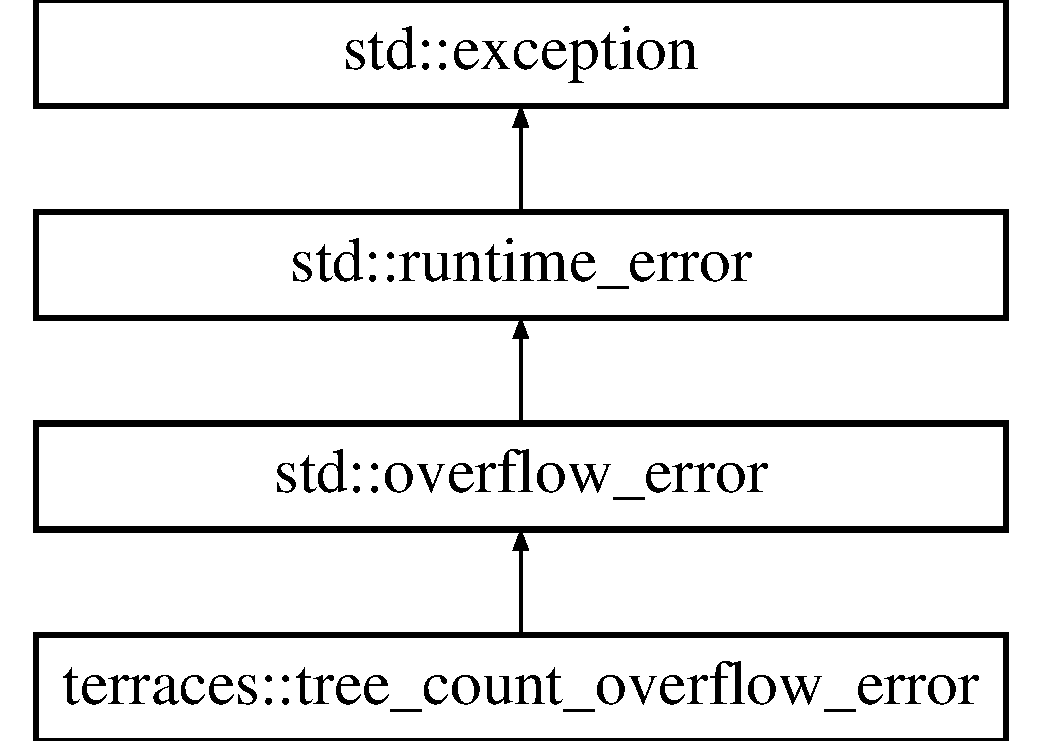
\includegraphics[height=4.000000cm]{classterraces_1_1tree__count__overflow__error}
\end{center}
\end{figure}


The documentation for this class was generated from the following file\+:\begin{DoxyCompactItemize}
\item 
include/terraces/\hyperlink{errors_8hpp}{errors.\+hpp}\end{DoxyCompactItemize}

\hypertarget{classterraces_1_1tree__cursor}{}\section{terraces\+:\+:tree\+\_\+cursor Class Reference}
\label{classterraces_1_1tree__cursor}\index{terraces\+::tree\+\_\+cursor@{terraces\+::tree\+\_\+cursor}}


{\ttfamily \#include $<$trees.\+hpp$>$}

\subsection*{Public Member Functions}
\begin{DoxyCompactItemize}
\item 
\hyperlink{classterraces_1_1tree__cursor_a454b86381c2e608f22d304b9a33d547c}{tree\+\_\+cursor} (\hyperlink{namespaceterraces_a07aaf7feec4a22c6cdefc14c5a81bdd0}{tree} \&t, \hyperlink{namespaceterraces_adbc33ccb543d1634e96d0eb02e472c77}{index} n)
\item 
\hyperlink{structterraces_1_1node}{node} \& \hyperlink{classterraces_1_1tree__cursor_aa84ad70d2231d809fb8730aea10c95e6}{get} () const
\item 
\hyperlink{structterraces_1_1node}{node} \& \hyperlink{classterraces_1_1tree__cursor_a992f9c4a4cf22b17f3908b2c39105f75}{operator$\ast$} () const
\item 
\hyperlink{namespaceterraces_adbc33ccb543d1634e96d0eb02e472c77}{index} \hyperlink{classterraces_1_1tree__cursor_af39b58768f4089f40919f107b2f85fa6}{get\+\_\+index} () const
\item 
bool \hyperlink{classterraces_1_1tree__cursor_ab34a83b29a7efed72b68aeb8623c1683}{has\+\_\+parent} () const
\item 
void \hyperlink{classterraces_1_1tree__cursor_a752d1a745ac3f5d9154cfc9cb307d465}{go\+\_\+parent} ()
\item 
bool \hyperlink{classterraces_1_1tree__cursor_aa9e8dc765ff85396ea388d8b77508a3c}{has\+\_\+lchild} () const
\item 
void \hyperlink{classterraces_1_1tree__cursor_ae6a8003188359d5bf8a68122ceadca4a}{go\+\_\+lchild} ()
\item 
bool \hyperlink{classterraces_1_1tree__cursor_aae66758d673a56247ffaca3628010013}{has\+\_\+rchild} () const
\item 
void \hyperlink{classterraces_1_1tree__cursor_ad27d7104eef00ab36a17e783705ec136}{go\+\_\+rchild} ()
\end{DoxyCompactItemize}


\subsection{Constructor \& Destructor Documentation}
\mbox{\Hypertarget{classterraces_1_1tree__cursor_a454b86381c2e608f22d304b9a33d547c}\label{classterraces_1_1tree__cursor_a454b86381c2e608f22d304b9a33d547c}} 
\index{terraces\+::tree\+\_\+cursor@{terraces\+::tree\+\_\+cursor}!tree\+\_\+cursor@{tree\+\_\+cursor}}
\index{tree\+\_\+cursor@{tree\+\_\+cursor}!terraces\+::tree\+\_\+cursor@{terraces\+::tree\+\_\+cursor}}
\subsubsection{\texorpdfstring{tree\+\_\+cursor()}{tree\_cursor()}}
{\footnotesize\ttfamily terraces\+::tree\+\_\+cursor\+::tree\+\_\+cursor (\begin{DoxyParamCaption}\item[{\hyperlink{namespaceterraces_a07aaf7feec4a22c6cdefc14c5a81bdd0}{tree} \&}]{t,  }\item[{\hyperlink{namespaceterraces_adbc33ccb543d1634e96d0eb02e472c77}{index}}]{n }\end{DoxyParamCaption})\hspace{0.3cm}{\ttfamily [inline]}}



\subsection{Member Function Documentation}
\mbox{\Hypertarget{classterraces_1_1tree__cursor_aa84ad70d2231d809fb8730aea10c95e6}\label{classterraces_1_1tree__cursor_aa84ad70d2231d809fb8730aea10c95e6}} 
\index{terraces\+::tree\+\_\+cursor@{terraces\+::tree\+\_\+cursor}!get@{get}}
\index{get@{get}!terraces\+::tree\+\_\+cursor@{terraces\+::tree\+\_\+cursor}}
\subsubsection{\texorpdfstring{get()}{get()}}
{\footnotesize\ttfamily \hyperlink{structterraces_1_1node}{node}\& terraces\+::tree\+\_\+cursor\+::get (\begin{DoxyParamCaption}{ }\end{DoxyParamCaption}) const\hspace{0.3cm}{\ttfamily [inline]}}

\mbox{\Hypertarget{classterraces_1_1tree__cursor_af39b58768f4089f40919f107b2f85fa6}\label{classterraces_1_1tree__cursor_af39b58768f4089f40919f107b2f85fa6}} 
\index{terraces\+::tree\+\_\+cursor@{terraces\+::tree\+\_\+cursor}!get\+\_\+index@{get\+\_\+index}}
\index{get\+\_\+index@{get\+\_\+index}!terraces\+::tree\+\_\+cursor@{terraces\+::tree\+\_\+cursor}}
\subsubsection{\texorpdfstring{get\+\_\+index()}{get\_index()}}
{\footnotesize\ttfamily \hyperlink{namespaceterraces_adbc33ccb543d1634e96d0eb02e472c77}{index} terraces\+::tree\+\_\+cursor\+::get\+\_\+index (\begin{DoxyParamCaption}{ }\end{DoxyParamCaption}) const\hspace{0.3cm}{\ttfamily [inline]}}

\mbox{\Hypertarget{classterraces_1_1tree__cursor_ae6a8003188359d5bf8a68122ceadca4a}\label{classterraces_1_1tree__cursor_ae6a8003188359d5bf8a68122ceadca4a}} 
\index{terraces\+::tree\+\_\+cursor@{terraces\+::tree\+\_\+cursor}!go\+\_\+lchild@{go\+\_\+lchild}}
\index{go\+\_\+lchild@{go\+\_\+lchild}!terraces\+::tree\+\_\+cursor@{terraces\+::tree\+\_\+cursor}}
\subsubsection{\texorpdfstring{go\+\_\+lchild()}{go\_lchild()}}
{\footnotesize\ttfamily void terraces\+::tree\+\_\+cursor\+::go\+\_\+lchild (\begin{DoxyParamCaption}{ }\end{DoxyParamCaption})\hspace{0.3cm}{\ttfamily [inline]}}

\mbox{\Hypertarget{classterraces_1_1tree__cursor_a752d1a745ac3f5d9154cfc9cb307d465}\label{classterraces_1_1tree__cursor_a752d1a745ac3f5d9154cfc9cb307d465}} 
\index{terraces\+::tree\+\_\+cursor@{terraces\+::tree\+\_\+cursor}!go\+\_\+parent@{go\+\_\+parent}}
\index{go\+\_\+parent@{go\+\_\+parent}!terraces\+::tree\+\_\+cursor@{terraces\+::tree\+\_\+cursor}}
\subsubsection{\texorpdfstring{go\+\_\+parent()}{go\_parent()}}
{\footnotesize\ttfamily void terraces\+::tree\+\_\+cursor\+::go\+\_\+parent (\begin{DoxyParamCaption}{ }\end{DoxyParamCaption})\hspace{0.3cm}{\ttfamily [inline]}}

\mbox{\Hypertarget{classterraces_1_1tree__cursor_ad27d7104eef00ab36a17e783705ec136}\label{classterraces_1_1tree__cursor_ad27d7104eef00ab36a17e783705ec136}} 
\index{terraces\+::tree\+\_\+cursor@{terraces\+::tree\+\_\+cursor}!go\+\_\+rchild@{go\+\_\+rchild}}
\index{go\+\_\+rchild@{go\+\_\+rchild}!terraces\+::tree\+\_\+cursor@{terraces\+::tree\+\_\+cursor}}
\subsubsection{\texorpdfstring{go\+\_\+rchild()}{go\_rchild()}}
{\footnotesize\ttfamily void terraces\+::tree\+\_\+cursor\+::go\+\_\+rchild (\begin{DoxyParamCaption}{ }\end{DoxyParamCaption})\hspace{0.3cm}{\ttfamily [inline]}}

\mbox{\Hypertarget{classterraces_1_1tree__cursor_aa9e8dc765ff85396ea388d8b77508a3c}\label{classterraces_1_1tree__cursor_aa9e8dc765ff85396ea388d8b77508a3c}} 
\index{terraces\+::tree\+\_\+cursor@{terraces\+::tree\+\_\+cursor}!has\+\_\+lchild@{has\+\_\+lchild}}
\index{has\+\_\+lchild@{has\+\_\+lchild}!terraces\+::tree\+\_\+cursor@{terraces\+::tree\+\_\+cursor}}
\subsubsection{\texorpdfstring{has\+\_\+lchild()}{has\_lchild()}}
{\footnotesize\ttfamily bool terraces\+::tree\+\_\+cursor\+::has\+\_\+lchild (\begin{DoxyParamCaption}{ }\end{DoxyParamCaption}) const\hspace{0.3cm}{\ttfamily [inline]}}

\mbox{\Hypertarget{classterraces_1_1tree__cursor_ab34a83b29a7efed72b68aeb8623c1683}\label{classterraces_1_1tree__cursor_ab34a83b29a7efed72b68aeb8623c1683}} 
\index{terraces\+::tree\+\_\+cursor@{terraces\+::tree\+\_\+cursor}!has\+\_\+parent@{has\+\_\+parent}}
\index{has\+\_\+parent@{has\+\_\+parent}!terraces\+::tree\+\_\+cursor@{terraces\+::tree\+\_\+cursor}}
\subsubsection{\texorpdfstring{has\+\_\+parent()}{has\_parent()}}
{\footnotesize\ttfamily bool terraces\+::tree\+\_\+cursor\+::has\+\_\+parent (\begin{DoxyParamCaption}{ }\end{DoxyParamCaption}) const\hspace{0.3cm}{\ttfamily [inline]}}

\mbox{\Hypertarget{classterraces_1_1tree__cursor_aae66758d673a56247ffaca3628010013}\label{classterraces_1_1tree__cursor_aae66758d673a56247ffaca3628010013}} 
\index{terraces\+::tree\+\_\+cursor@{terraces\+::tree\+\_\+cursor}!has\+\_\+rchild@{has\+\_\+rchild}}
\index{has\+\_\+rchild@{has\+\_\+rchild}!terraces\+::tree\+\_\+cursor@{terraces\+::tree\+\_\+cursor}}
\subsubsection{\texorpdfstring{has\+\_\+rchild()}{has\_rchild()}}
{\footnotesize\ttfamily bool terraces\+::tree\+\_\+cursor\+::has\+\_\+rchild (\begin{DoxyParamCaption}{ }\end{DoxyParamCaption}) const\hspace{0.3cm}{\ttfamily [inline]}}

\mbox{\Hypertarget{classterraces_1_1tree__cursor_a992f9c4a4cf22b17f3908b2c39105f75}\label{classterraces_1_1tree__cursor_a992f9c4a4cf22b17f3908b2c39105f75}} 
\index{terraces\+::tree\+\_\+cursor@{terraces\+::tree\+\_\+cursor}!operator$\ast$@{operator$\ast$}}
\index{operator$\ast$@{operator$\ast$}!terraces\+::tree\+\_\+cursor@{terraces\+::tree\+\_\+cursor}}
\subsubsection{\texorpdfstring{operator$\ast$()}{operator*()}}
{\footnotesize\ttfamily \hyperlink{structterraces_1_1node}{node}\& terraces\+::tree\+\_\+cursor\+::operator$\ast$ (\begin{DoxyParamCaption}{ }\end{DoxyParamCaption}) const\hspace{0.3cm}{\ttfamily [inline]}}



The documentation for this class was generated from the following file\+:\begin{DoxyCompactItemize}
\item 
include/terraces/\hyperlink{trees_8hpp}{trees.\+hpp}\end{DoxyCompactItemize}

\hypertarget{classterraces_1_1tree__enumerator}{}\section{terraces\+:\+:tree\+\_\+enumerator$<$ Callback, Parallel $>$ Class Template Reference}
\label{classterraces_1_1tree__enumerator}\index{terraces\+::tree\+\_\+enumerator$<$ Callback, Parallel $>$@{terraces\+::tree\+\_\+enumerator$<$ Callback, Parallel $>$}}


{\ttfamily \#include $<$supertree\+\_\+enumerator.\+hpp$>$}

\subsection*{Public Member Functions}
\begin{DoxyCompactItemize}
\item 
\hyperlink{classterraces_1_1tree__enumerator_abac88ae38b6f65882007d15d4a4fc213}{tree\+\_\+enumerator} (Callback cb, \hyperlink{namespaceterraces_adbc33ccb543d1634e96d0eb02e472c77}{index} leaf\+\_\+count, \hyperlink{namespaceterraces_adbc33ccb543d1634e96d0eb02e472c77}{index} constraint\+\_\+count)
\item 
result\+\_\+type \hyperlink{classterraces_1_1tree__enumerator_ae523d14dfc46be4015d4ba5993f4c2ba}{run} (\hyperlink{namespaceterraces_adbc33ccb543d1634e96d0eb02e472c77}{index} num\+\_\+leaves, const \hyperlink{namespaceterraces_a6f603ffd30ed4d902fce6424492e0581}{constraints} \&\hyperlink{namespaceterraces_a6f603ffd30ed4d902fce6424492e0581}{constraints}, \hyperlink{namespaceterraces_adbc33ccb543d1634e96d0eb02e472c77}{index} root\+\_\+leaf)
\item 
result\+\_\+type \hyperlink{classterraces_1_1tree__enumerator_a933db3e1e37840e6a217bc1faca3194b}{run} (\hyperlink{namespaceterraces_adbc33ccb543d1634e96d0eb02e472c77}{index} num\+\_\+leaves, const \hyperlink{namespaceterraces_a6f603ffd30ed4d902fce6424492e0581}{constraints} \&\hyperlink{namespaceterraces_a6f603ffd30ed4d902fce6424492e0581}{constraints})
\item 
result\+\_\+type \hyperlink{classterraces_1_1tree__enumerator_a7d5262aee9bc2a40318b39314838dc92}{run} (const \hyperlink{namespaceterraces_acc45ec9c561024c50ecbce5b6738ba08}{ranked\+\_\+bitvector} \&leaves, const \hyperlink{namespaceterraces_a1b526fb554dff829f7ad51eb21d5ed06}{bitvector} \&constraint\+\_\+occ)
\item 
const Callback \& \hyperlink{classterraces_1_1tree__enumerator_a050104cc4faec501e8329c427730e372}{callback} () const
\item 
const Callback \& \hyperlink{classterraces_1_1tree__enumerator_a21af6b1b63002d05ce90f8100521d858}{parallel\+\_\+callback} (\hyperlink{namespaceterraces_adbc33ccb543d1634e96d0eb02e472c77}{index} thread) const
\end{DoxyCompactItemize}
\subsection*{Friends}
\begin{DoxyCompactItemize}
\item 
class \hyperlink{classterraces_1_1tree__enumerator_a9233453e725dd710bc8d92a5291f832b}{tree\+\_\+enumerator$<$ Callback, true $>$}
\end{DoxyCompactItemize}


\subsection{Constructor \& Destructor Documentation}
\mbox{\Hypertarget{classterraces_1_1tree__enumerator_abac88ae38b6f65882007d15d4a4fc213}\label{classterraces_1_1tree__enumerator_abac88ae38b6f65882007d15d4a4fc213}} 
\index{terraces\+::tree\+\_\+enumerator@{terraces\+::tree\+\_\+enumerator}!tree\+\_\+enumerator@{tree\+\_\+enumerator}}
\index{tree\+\_\+enumerator@{tree\+\_\+enumerator}!terraces\+::tree\+\_\+enumerator@{terraces\+::tree\+\_\+enumerator}}
\subsubsection{\texorpdfstring{tree\+\_\+enumerator()}{tree\_enumerator()}}
{\footnotesize\ttfamily template$<$typename Callback, bool Parallel$>$ \\
\hyperlink{classterraces_1_1tree__enumerator}{terraces\+::tree\+\_\+enumerator}$<$ Callback, Parallel $>$\+::\hyperlink{classterraces_1_1tree__enumerator}{tree\+\_\+enumerator} (\begin{DoxyParamCaption}\item[{Callback}]{cb,  }\item[{\hyperlink{namespaceterraces_adbc33ccb543d1634e96d0eb02e472c77}{index}}]{leaf\+\_\+count,  }\item[{\hyperlink{namespaceterraces_adbc33ccb543d1634e96d0eb02e472c77}{index}}]{constraint\+\_\+count }\end{DoxyParamCaption})}



\subsection{Member Function Documentation}
\mbox{\Hypertarget{classterraces_1_1tree__enumerator_a050104cc4faec501e8329c427730e372}\label{classterraces_1_1tree__enumerator_a050104cc4faec501e8329c427730e372}} 
\index{terraces\+::tree\+\_\+enumerator@{terraces\+::tree\+\_\+enumerator}!callback@{callback}}
\index{callback@{callback}!terraces\+::tree\+\_\+enumerator@{terraces\+::tree\+\_\+enumerator}}
\subsubsection{\texorpdfstring{callback()}{callback()}}
{\footnotesize\ttfamily template$<$typename Callback, bool Parallel = false$>$ \\
const Callback\& \hyperlink{classterraces_1_1tree__enumerator}{terraces\+::tree\+\_\+enumerator}$<$ Callback, Parallel $>$\+::callback (\begin{DoxyParamCaption}{ }\end{DoxyParamCaption}) const\hspace{0.3cm}{\ttfamily [inline]}}

\mbox{\Hypertarget{classterraces_1_1tree__enumerator_a21af6b1b63002d05ce90f8100521d858}\label{classterraces_1_1tree__enumerator_a21af6b1b63002d05ce90f8100521d858}} 
\index{terraces\+::tree\+\_\+enumerator@{terraces\+::tree\+\_\+enumerator}!parallel\+\_\+callback@{parallel\+\_\+callback}}
\index{parallel\+\_\+callback@{parallel\+\_\+callback}!terraces\+::tree\+\_\+enumerator@{terraces\+::tree\+\_\+enumerator}}
\subsubsection{\texorpdfstring{parallel\+\_\+callback()}{parallel\_callback()}}
{\footnotesize\ttfamily template$<$typename Callback, bool Parallel = false$>$ \\
const Callback\& \hyperlink{classterraces_1_1tree__enumerator}{terraces\+::tree\+\_\+enumerator}$<$ Callback, Parallel $>$\+::parallel\+\_\+callback (\begin{DoxyParamCaption}\item[{\hyperlink{namespaceterraces_adbc33ccb543d1634e96d0eb02e472c77}{index}}]{thread }\end{DoxyParamCaption}) const\hspace{0.3cm}{\ttfamily [inline]}}

\mbox{\Hypertarget{classterraces_1_1tree__enumerator_ae523d14dfc46be4015d4ba5993f4c2ba}\label{classterraces_1_1tree__enumerator_ae523d14dfc46be4015d4ba5993f4c2ba}} 
\index{terraces\+::tree\+\_\+enumerator@{terraces\+::tree\+\_\+enumerator}!run@{run}}
\index{run@{run}!terraces\+::tree\+\_\+enumerator@{terraces\+::tree\+\_\+enumerator}}
\subsubsection{\texorpdfstring{run()}{run()}\hspace{0.1cm}{\footnotesize\ttfamily [1/3]}}
{\footnotesize\ttfamily template$<$typename Callback , bool Parallel$>$ \\
auto \hyperlink{classterraces_1_1tree__enumerator}{terraces\+::tree\+\_\+enumerator}$<$ Callback, Parallel $>$\+::run (\begin{DoxyParamCaption}\item[{\hyperlink{namespaceterraces_adbc33ccb543d1634e96d0eb02e472c77}{index}}]{num\+\_\+leaves,  }\item[{const \hyperlink{namespaceterraces_a6f603ffd30ed4d902fce6424492e0581}{constraints} \&}]{constraints,  }\item[{\hyperlink{namespaceterraces_adbc33ccb543d1634e96d0eb02e472c77}{index}}]{root\+\_\+leaf }\end{DoxyParamCaption})}

\mbox{\Hypertarget{classterraces_1_1tree__enumerator_a933db3e1e37840e6a217bc1faca3194b}\label{classterraces_1_1tree__enumerator_a933db3e1e37840e6a217bc1faca3194b}} 
\index{terraces\+::tree\+\_\+enumerator@{terraces\+::tree\+\_\+enumerator}!run@{run}}
\index{run@{run}!terraces\+::tree\+\_\+enumerator@{terraces\+::tree\+\_\+enumerator}}
\subsubsection{\texorpdfstring{run()}{run()}\hspace{0.1cm}{\footnotesize\ttfamily [2/3]}}
{\footnotesize\ttfamily template$<$typename Callback , bool Parallel$>$ \\
auto \hyperlink{classterraces_1_1tree__enumerator}{terraces\+::tree\+\_\+enumerator}$<$ Callback, Parallel $>$\+::run (\begin{DoxyParamCaption}\item[{\hyperlink{namespaceterraces_adbc33ccb543d1634e96d0eb02e472c77}{index}}]{num\+\_\+leaves,  }\item[{const \hyperlink{namespaceterraces_a6f603ffd30ed4d902fce6424492e0581}{constraints} \&}]{constraints }\end{DoxyParamCaption})}

\mbox{\Hypertarget{classterraces_1_1tree__enumerator_a7d5262aee9bc2a40318b39314838dc92}\label{classterraces_1_1tree__enumerator_a7d5262aee9bc2a40318b39314838dc92}} 
\index{terraces\+::tree\+\_\+enumerator@{terraces\+::tree\+\_\+enumerator}!run@{run}}
\index{run@{run}!terraces\+::tree\+\_\+enumerator@{terraces\+::tree\+\_\+enumerator}}
\subsubsection{\texorpdfstring{run()}{run()}\hspace{0.1cm}{\footnotesize\ttfamily [3/3]}}
{\footnotesize\ttfamily template$<$typename Callback , bool Parallel$>$ \\
auto \hyperlink{classterraces_1_1tree__enumerator}{terraces\+::tree\+\_\+enumerator}$<$ Callback, Parallel $>$\+::run (\begin{DoxyParamCaption}\item[{const \hyperlink{namespaceterraces_acc45ec9c561024c50ecbce5b6738ba08}{ranked\+\_\+bitvector} \&}]{leaves,  }\item[{const \hyperlink{namespaceterraces_a1b526fb554dff829f7ad51eb21d5ed06}{bitvector} \&}]{constraint\+\_\+occ }\end{DoxyParamCaption})}



\subsection{Friends And Related Function Documentation}
\mbox{\Hypertarget{classterraces_1_1tree__enumerator_a9233453e725dd710bc8d92a5291f832b}\label{classterraces_1_1tree__enumerator_a9233453e725dd710bc8d92a5291f832b}} 
\index{terraces\+::tree\+\_\+enumerator@{terraces\+::tree\+\_\+enumerator}!tree\+\_\+enumerator$<$ Callback, true $>$@{tree\+\_\+enumerator$<$ Callback, true $>$}}
\index{tree\+\_\+enumerator$<$ Callback, true $>$@{tree\+\_\+enumerator$<$ Callback, true $>$}!terraces\+::tree\+\_\+enumerator@{terraces\+::tree\+\_\+enumerator}}
\subsubsection{\texorpdfstring{tree\+\_\+enumerator$<$ Callback, true $>$}{tree\_enumerator< Callback, true >}}
{\footnotesize\ttfamily template$<$typename Callback, bool Parallel = false$>$ \\
friend class \hyperlink{classterraces_1_1tree__enumerator}{tree\+\_\+enumerator}$<$ Callback, true $>$\hspace{0.3cm}{\ttfamily [friend]}}



The documentation for this class was generated from the following file\+:\begin{DoxyCompactItemize}
\item 
lib/\hyperlink{supertree__enumerator_8hpp}{supertree\+\_\+enumerator.\+hpp}\end{DoxyCompactItemize}

\hypertarget{structtree__node}{}\section{tree\+\_\+node Struct Reference}
\label{structtree__node}\index{tree\+\_\+node@{tree\+\_\+node}}
\subsection*{Public Member Functions}
\begin{DoxyCompactItemize}
\item 
\hyperlink{structtree__node_a835de19906d9a6b2f2c8f20345be4839}{tree\+\_\+node} (\hyperlink{tree__gen_8cpp_a7376ecf9f645bcbaa2f0459e17d7588f}{index} \hyperlink{structtree__node_ab8bbd1b843e135810fc96529bc452d22}{parent}=none, \hyperlink{tree__gen_8cpp_a7376ecf9f645bcbaa2f0459e17d7588f}{index} \hyperlink{structtree__node_a6ee3ea07f568423adde3b6911ea3b041}{left}=none, \hyperlink{tree__gen_8cpp_a7376ecf9f645bcbaa2f0459e17d7588f}{index} \hyperlink{structtree__node_a244a10f0fa615392414c301291ba2c47}{right}=none)
\item 
void \hyperlink{structtree__node_acd3e8c452abe8574fbf7b2d1ce52ccfc}{set\+\_\+children} (\hyperlink{tree__gen_8cpp_a7376ecf9f645bcbaa2f0459e17d7588f}{index} l, \hyperlink{tree__gen_8cpp_a7376ecf9f645bcbaa2f0459e17d7588f}{index} r)
\item 
bool \hyperlink{structtree__node_a2c35968103d4326090dcd4b100c1fd56}{is\+\_\+leaf} () const
\end{DoxyCompactItemize}
\subsection*{Public Attributes}
\begin{DoxyCompactItemize}
\item 
\hyperlink{tree__gen_8cpp_a7376ecf9f645bcbaa2f0459e17d7588f}{index} \hyperlink{structtree__node_ab8bbd1b843e135810fc96529bc452d22}{parent} = none
\item 
\hyperlink{tree__gen_8cpp_a7376ecf9f645bcbaa2f0459e17d7588f}{index} \hyperlink{structtree__node_a6ee3ea07f568423adde3b6911ea3b041}{left} = none
\item 
\hyperlink{tree__gen_8cpp_a7376ecf9f645bcbaa2f0459e17d7588f}{index} \hyperlink{structtree__node_a244a10f0fa615392414c301291ba2c47}{right} = none
\item 
std\+::uint8\+\_\+t \hyperlink{structtree__node_a2cd221687b1d31a8d5e78a754b1cb53c}{visited} = 0u
\end{DoxyCompactItemize}


\subsection{Constructor \& Destructor Documentation}
\mbox{\Hypertarget{structtree__node_a835de19906d9a6b2f2c8f20345be4839}\label{structtree__node_a835de19906d9a6b2f2c8f20345be4839}} 
\index{tree\+\_\+node@{tree\+\_\+node}!tree\+\_\+node@{tree\+\_\+node}}
\index{tree\+\_\+node@{tree\+\_\+node}!tree\+\_\+node@{tree\+\_\+node}}
\subsubsection{\texorpdfstring{tree\+\_\+node()}{tree\_node()}}
{\footnotesize\ttfamily tree\+\_\+node\+::tree\+\_\+node (\begin{DoxyParamCaption}\item[{\hyperlink{tree__gen_8cpp_a7376ecf9f645bcbaa2f0459e17d7588f}{index}}]{parent = {\ttfamily none},  }\item[{\hyperlink{tree__gen_8cpp_a7376ecf9f645bcbaa2f0459e17d7588f}{index}}]{left = {\ttfamily none},  }\item[{\hyperlink{tree__gen_8cpp_a7376ecf9f645bcbaa2f0459e17d7588f}{index}}]{right = {\ttfamily none} }\end{DoxyParamCaption})\hspace{0.3cm}{\ttfamily [inline]}, {\ttfamily [explicit]}}



\subsection{Member Function Documentation}
\mbox{\Hypertarget{structtree__node_a2c35968103d4326090dcd4b100c1fd56}\label{structtree__node_a2c35968103d4326090dcd4b100c1fd56}} 
\index{tree\+\_\+node@{tree\+\_\+node}!is\+\_\+leaf@{is\+\_\+leaf}}
\index{is\+\_\+leaf@{is\+\_\+leaf}!tree\+\_\+node@{tree\+\_\+node}}
\subsubsection{\texorpdfstring{is\+\_\+leaf()}{is\_leaf()}}
{\footnotesize\ttfamily bool tree\+\_\+node\+::is\+\_\+leaf (\begin{DoxyParamCaption}{ }\end{DoxyParamCaption}) const\hspace{0.3cm}{\ttfamily [inline]}}

\mbox{\Hypertarget{structtree__node_acd3e8c452abe8574fbf7b2d1ce52ccfc}\label{structtree__node_acd3e8c452abe8574fbf7b2d1ce52ccfc}} 
\index{tree\+\_\+node@{tree\+\_\+node}!set\+\_\+children@{set\+\_\+children}}
\index{set\+\_\+children@{set\+\_\+children}!tree\+\_\+node@{tree\+\_\+node}}
\subsubsection{\texorpdfstring{set\+\_\+children()}{set\_children()}}
{\footnotesize\ttfamily void tree\+\_\+node\+::set\+\_\+children (\begin{DoxyParamCaption}\item[{\hyperlink{tree__gen_8cpp_a7376ecf9f645bcbaa2f0459e17d7588f}{index}}]{l,  }\item[{\hyperlink{tree__gen_8cpp_a7376ecf9f645bcbaa2f0459e17d7588f}{index}}]{r }\end{DoxyParamCaption})\hspace{0.3cm}{\ttfamily [inline]}}



\subsection{Member Data Documentation}
\mbox{\Hypertarget{structtree__node_a6ee3ea07f568423adde3b6911ea3b041}\label{structtree__node_a6ee3ea07f568423adde3b6911ea3b041}} 
\index{tree\+\_\+node@{tree\+\_\+node}!left@{left}}
\index{left@{left}!tree\+\_\+node@{tree\+\_\+node}}
\subsubsection{\texorpdfstring{left}{left}}
{\footnotesize\ttfamily \hyperlink{tree__gen_8cpp_a7376ecf9f645bcbaa2f0459e17d7588f}{index} tree\+\_\+node\+::left = none}

\mbox{\Hypertarget{structtree__node_ab8bbd1b843e135810fc96529bc452d22}\label{structtree__node_ab8bbd1b843e135810fc96529bc452d22}} 
\index{tree\+\_\+node@{tree\+\_\+node}!parent@{parent}}
\index{parent@{parent}!tree\+\_\+node@{tree\+\_\+node}}
\subsubsection{\texorpdfstring{parent}{parent}}
{\footnotesize\ttfamily \hyperlink{tree__gen_8cpp_a7376ecf9f645bcbaa2f0459e17d7588f}{index} tree\+\_\+node\+::parent = none}

\mbox{\Hypertarget{structtree__node_a244a10f0fa615392414c301291ba2c47}\label{structtree__node_a244a10f0fa615392414c301291ba2c47}} 
\index{tree\+\_\+node@{tree\+\_\+node}!right@{right}}
\index{right@{right}!tree\+\_\+node@{tree\+\_\+node}}
\subsubsection{\texorpdfstring{right}{right}}
{\footnotesize\ttfamily \hyperlink{tree__gen_8cpp_a7376ecf9f645bcbaa2f0459e17d7588f}{index} tree\+\_\+node\+::right = none}

\mbox{\Hypertarget{structtree__node_a2cd221687b1d31a8d5e78a754b1cb53c}\label{structtree__node_a2cd221687b1d31a8d5e78a754b1cb53c}} 
\index{tree\+\_\+node@{tree\+\_\+node}!visited@{visited}}
\index{visited@{visited}!tree\+\_\+node@{tree\+\_\+node}}
\subsubsection{\texorpdfstring{visited}{visited}}
{\footnotesize\ttfamily std\+::uint8\+\_\+t tree\+\_\+node\+::visited = 0u}



The documentation for this struct was generated from the following file\+:\begin{DoxyCompactItemize}
\item 
app/\hyperlink{tree__gen_8cpp}{tree\+\_\+gen.\+cpp}\end{DoxyCompactItemize}

\hypertarget{structterraces_1_1tree__set}{}\section{terraces\+:\+:tree\+\_\+set Struct Reference}
\label{structterraces_1_1tree__set}\index{terraces\+::tree\+\_\+set@{terraces\+::tree\+\_\+set}}


{\ttfamily \#include $<$parser.\+hpp$>$}

\subsection*{Public Attributes}
\begin{DoxyCompactItemize}
\item 
\hyperlink{namespaceterraces_a07aaf7feec4a22c6cdefc14c5a81bdd0}{terraces\+::tree} \hyperlink{structterraces_1_1tree__set_abdce12c87cab9633ad5f8ae735ce6007}{tree}
\item 
\hyperlink{namespaceterraces_a4ef0217fe5aed881737d9bc5a8d45dca}{name\+\_\+map} \hyperlink{structterraces_1_1tree__set_ab9ca9d14518314055ffb7ea450bacc6b}{names}
\item 
\hyperlink{namespaceterraces_a148f3e895119c2a72d995caae669e40d}{index\+\_\+map} \hyperlink{structterraces_1_1tree__set_a35996bc322c09773259be8b51b1944fa}{indices}
\end{DoxyCompactItemize}


\subsection{Member Data Documentation}
\mbox{\Hypertarget{structterraces_1_1tree__set_a35996bc322c09773259be8b51b1944fa}\label{structterraces_1_1tree__set_a35996bc322c09773259be8b51b1944fa}} 
\index{terraces\+::tree\+\_\+set@{terraces\+::tree\+\_\+set}!indices@{indices}}
\index{indices@{indices}!terraces\+::tree\+\_\+set@{terraces\+::tree\+\_\+set}}
\subsubsection{\texorpdfstring{indices}{indices}}
{\footnotesize\ttfamily \hyperlink{namespaceterraces_a148f3e895119c2a72d995caae669e40d}{index\+\_\+map} terraces\+::tree\+\_\+set\+::indices}

\mbox{\Hypertarget{structterraces_1_1tree__set_ab9ca9d14518314055ffb7ea450bacc6b}\label{structterraces_1_1tree__set_ab9ca9d14518314055ffb7ea450bacc6b}} 
\index{terraces\+::tree\+\_\+set@{terraces\+::tree\+\_\+set}!names@{names}}
\index{names@{names}!terraces\+::tree\+\_\+set@{terraces\+::tree\+\_\+set}}
\subsubsection{\texorpdfstring{names}{names}}
{\footnotesize\ttfamily \hyperlink{namespaceterraces_a4ef0217fe5aed881737d9bc5a8d45dca}{name\+\_\+map} terraces\+::tree\+\_\+set\+::names}

\mbox{\Hypertarget{structterraces_1_1tree__set_abdce12c87cab9633ad5f8ae735ce6007}\label{structterraces_1_1tree__set_abdce12c87cab9633ad5f8ae735ce6007}} 
\index{terraces\+::tree\+\_\+set@{terraces\+::tree\+\_\+set}!tree@{tree}}
\index{tree@{tree}!terraces\+::tree\+\_\+set@{terraces\+::tree\+\_\+set}}
\subsubsection{\texorpdfstring{tree}{tree}}
{\footnotesize\ttfamily \hyperlink{namespaceterraces_a07aaf7feec4a22c6cdefc14c5a81bdd0}{terraces\+::tree} terraces\+::tree\+\_\+set\+::tree}



The documentation for this struct was generated from the following file\+:\begin{DoxyCompactItemize}
\item 
include/terraces/\hyperlink{parser_8hpp}{parser.\+hpp}\end{DoxyCompactItemize}

\hypertarget{structterraces_1_1multitree__nodes_1_1unconstrained}{}\section{terraces\+:\+:multitree\+\_\+nodes\+:\+:unconstrained Struct Reference}
\label{structterraces_1_1multitree__nodes_1_1unconstrained}\index{terraces\+::multitree\+\_\+nodes\+::unconstrained@{terraces\+::multitree\+\_\+nodes\+::unconstrained}}


{\ttfamily \#include $<$multitree.\+hpp$>$}

\subsection*{Public Attributes}
\begin{DoxyCompactItemize}
\item 
\hyperlink{namespaceterraces_adbc33ccb543d1634e96d0eb02e472c77}{index} $\ast$ \hyperlink{structterraces_1_1multitree__nodes_1_1unconstrained_a682b1bc98947bba76df87c098f87962a}{begin}
\item 
\hyperlink{namespaceterraces_adbc33ccb543d1634e96d0eb02e472c77}{index} $\ast$ \hyperlink{structterraces_1_1multitree__nodes_1_1unconstrained_a09312cac542aacde054f495a914f6cab}{end}
\end{DoxyCompactItemize}


\subsection{Member Data Documentation}
\mbox{\Hypertarget{structterraces_1_1multitree__nodes_1_1unconstrained_a682b1bc98947bba76df87c098f87962a}\label{structterraces_1_1multitree__nodes_1_1unconstrained_a682b1bc98947bba76df87c098f87962a}} 
\index{terraces\+::multitree\+\_\+nodes\+::unconstrained@{terraces\+::multitree\+\_\+nodes\+::unconstrained}!begin@{begin}}
\index{begin@{begin}!terraces\+::multitree\+\_\+nodes\+::unconstrained@{terraces\+::multitree\+\_\+nodes\+::unconstrained}}
\subsubsection{\texorpdfstring{begin}{begin}}
{\footnotesize\ttfamily \hyperlink{namespaceterraces_adbc33ccb543d1634e96d0eb02e472c77}{index}$\ast$ terraces\+::multitree\+\_\+nodes\+::unconstrained\+::begin}

\mbox{\Hypertarget{structterraces_1_1multitree__nodes_1_1unconstrained_a09312cac542aacde054f495a914f6cab}\label{structterraces_1_1multitree__nodes_1_1unconstrained_a09312cac542aacde054f495a914f6cab}} 
\index{terraces\+::multitree\+\_\+nodes\+::unconstrained@{terraces\+::multitree\+\_\+nodes\+::unconstrained}!end@{end}}
\index{end@{end}!terraces\+::multitree\+\_\+nodes\+::unconstrained@{terraces\+::multitree\+\_\+nodes\+::unconstrained}}
\subsubsection{\texorpdfstring{end}{end}}
{\footnotesize\ttfamily \hyperlink{namespaceterraces_adbc33ccb543d1634e96d0eb02e472c77}{index}$\ast$ terraces\+::multitree\+\_\+nodes\+::unconstrained\+::end}



The documentation for this struct was generated from the following file\+:\begin{DoxyCompactItemize}
\item 
include/terraces/\hyperlink{multitree_8hpp}{multitree.\+hpp}\end{DoxyCompactItemize}

\hypertarget{structterraces_1_1multitree__nodes_1_1unexplored}{}\section{terraces\+:\+:multitree\+\_\+nodes\+:\+:unexplored Struct Reference}
\label{structterraces_1_1multitree__nodes_1_1unexplored}\index{terraces\+::multitree\+\_\+nodes\+::unexplored@{terraces\+::multitree\+\_\+nodes\+::unexplored}}


{\ttfamily \#include $<$multitree.\+hpp$>$}

\subsection*{Public Attributes}
\begin{DoxyCompactItemize}
\item 
\hyperlink{namespaceterraces_adbc33ccb543d1634e96d0eb02e472c77}{index} $\ast$ \hyperlink{structterraces_1_1multitree__nodes_1_1unexplored_ab5ec32670aaf0966777e2e0ca2ec9a6e}{begin}
\item 
\hyperlink{namespaceterraces_adbc33ccb543d1634e96d0eb02e472c77}{index} $\ast$ \hyperlink{structterraces_1_1multitree__nodes_1_1unexplored_afaa1f07beef3f328f44b778dc9d222eb}{end}
\end{DoxyCompactItemize}


\subsection{Member Data Documentation}
\mbox{\Hypertarget{structterraces_1_1multitree__nodes_1_1unexplored_ab5ec32670aaf0966777e2e0ca2ec9a6e}\label{structterraces_1_1multitree__nodes_1_1unexplored_ab5ec32670aaf0966777e2e0ca2ec9a6e}} 
\index{terraces\+::multitree\+\_\+nodes\+::unexplored@{terraces\+::multitree\+\_\+nodes\+::unexplored}!begin@{begin}}
\index{begin@{begin}!terraces\+::multitree\+\_\+nodes\+::unexplored@{terraces\+::multitree\+\_\+nodes\+::unexplored}}
\subsubsection{\texorpdfstring{begin}{begin}}
{\footnotesize\ttfamily \hyperlink{namespaceterraces_adbc33ccb543d1634e96d0eb02e472c77}{index}$\ast$ terraces\+::multitree\+\_\+nodes\+::unexplored\+::begin}

\mbox{\Hypertarget{structterraces_1_1multitree__nodes_1_1unexplored_afaa1f07beef3f328f44b778dc9d222eb}\label{structterraces_1_1multitree__nodes_1_1unexplored_afaa1f07beef3f328f44b778dc9d222eb}} 
\index{terraces\+::multitree\+\_\+nodes\+::unexplored@{terraces\+::multitree\+\_\+nodes\+::unexplored}!end@{end}}
\index{end@{end}!terraces\+::multitree\+\_\+nodes\+::unexplored@{terraces\+::multitree\+\_\+nodes\+::unexplored}}
\subsubsection{\texorpdfstring{end}{end}}
{\footnotesize\ttfamily \hyperlink{namespaceterraces_adbc33ccb543d1634e96d0eb02e472c77}{index}$\ast$ terraces\+::multitree\+\_\+nodes\+::unexplored\+::end}



The documentation for this struct was generated from the following file\+:\begin{DoxyCompactItemize}
\item 
include/terraces/\hyperlink{multitree_8hpp}{multitree.\+hpp}\end{DoxyCompactItemize}

\hypertarget{classterraces_1_1union__find}{}\section{terraces\+:\+:union\+\_\+find Class Reference}
\label{classterraces_1_1union__find}\index{terraces\+::union\+\_\+find@{terraces\+::union\+\_\+find}}


{\ttfamily \#include $<$union\+\_\+find.\+hpp$>$}

\subsection*{Public Types}
\begin{DoxyCompactItemize}
\item 
using \hyperlink{classterraces_1_1union__find_a72c65370f63e73215aad5d3ffdde3e55}{value\+\_\+type} = \hyperlink{namespaceterraces_adbc33ccb543d1634e96d0eb02e472c77}{index}
\end{DoxyCompactItemize}
\subsection*{Public Member Functions}
\begin{DoxyCompactItemize}
\item 
\hyperlink{classterraces_1_1union__find_a6a2c8c169e8c19b55c78b8e426d3d7b6}{union\+\_\+find} (\hyperlink{namespaceterraces_adbc33ccb543d1634e96d0eb02e472c77}{index}, \hyperlink{classterraces_1_1utils_1_1stack__allocator}{utils\+::stack\+\_\+allocator}$<$ \hyperlink{namespaceterraces_adbc33ccb543d1634e96d0eb02e472c77}{index} $>$ a)
\item 
\hyperlink{namespaceterraces_adbc33ccb543d1634e96d0eb02e472c77}{index} \hyperlink{classterraces_1_1union__find_a2517df18689c278dc41f14395cd36f5e}{find} (\hyperlink{namespaceterraces_adbc33ccb543d1634e96d0eb02e472c77}{index})
\item 
\hyperlink{namespaceterraces_adbc33ccb543d1634e96d0eb02e472c77}{index} \hyperlink{classterraces_1_1union__find_ab873ad737cf121e74b2aa644006c35ee}{simple\+\_\+find} (\hyperlink{namespaceterraces_adbc33ccb543d1634e96d0eb02e472c77}{index} x) const
\item 
\hyperlink{namespaceterraces_adbc33ccb543d1634e96d0eb02e472c77}{index} \hyperlink{classterraces_1_1union__find_ae76d167c5073215dc310720bfc619d8d}{size} () const
\item 
void \hyperlink{classterraces_1_1union__find_a8c6d1cabc854aedf4b04c6047680b03c}{compress} ()
\item 
void \hyperlink{classterraces_1_1union__find_a27e4ea548412d40c25904739d21e41ca}{merge} (\hyperlink{namespaceterraces_adbc33ccb543d1634e96d0eb02e472c77}{index}, \hyperlink{namespaceterraces_adbc33ccb543d1634e96d0eb02e472c77}{index})
\item 
bool \hyperlink{classterraces_1_1union__find_a6659180419525421c0d4ff6c7e48fc47}{is\+\_\+representative} (\hyperlink{namespaceterraces_adbc33ccb543d1634e96d0eb02e472c77}{index} x) const
\end{DoxyCompactItemize}


\subsection{Member Typedef Documentation}
\mbox{\Hypertarget{classterraces_1_1union__find_a72c65370f63e73215aad5d3ffdde3e55}\label{classterraces_1_1union__find_a72c65370f63e73215aad5d3ffdde3e55}} 
\index{terraces\+::union\+\_\+find@{terraces\+::union\+\_\+find}!value\+\_\+type@{value\+\_\+type}}
\index{value\+\_\+type@{value\+\_\+type}!terraces\+::union\+\_\+find@{terraces\+::union\+\_\+find}}
\subsubsection{\texorpdfstring{value\+\_\+type}{value\_type}}
{\footnotesize\ttfamily using \hyperlink{classterraces_1_1union__find_a72c65370f63e73215aad5d3ffdde3e55}{terraces\+::union\+\_\+find\+::value\+\_\+type} =  \hyperlink{namespaceterraces_adbc33ccb543d1634e96d0eb02e472c77}{index}}



\subsection{Constructor \& Destructor Documentation}
\mbox{\Hypertarget{classterraces_1_1union__find_a6a2c8c169e8c19b55c78b8e426d3d7b6}\label{classterraces_1_1union__find_a6a2c8c169e8c19b55c78b8e426d3d7b6}} 
\index{terraces\+::union\+\_\+find@{terraces\+::union\+\_\+find}!union\+\_\+find@{union\+\_\+find}}
\index{union\+\_\+find@{union\+\_\+find}!terraces\+::union\+\_\+find@{terraces\+::union\+\_\+find}}
\subsubsection{\texorpdfstring{union\+\_\+find()}{union\_find()}}
{\footnotesize\ttfamily terraces\+::union\+\_\+find\+::union\+\_\+find (\begin{DoxyParamCaption}\item[{\hyperlink{namespaceterraces_adbc33ccb543d1634e96d0eb02e472c77}{index}}]{n,  }\item[{\hyperlink{classterraces_1_1utils_1_1stack__allocator}{utils\+::stack\+\_\+allocator}$<$ \hyperlink{namespaceterraces_adbc33ccb543d1634e96d0eb02e472c77}{index} $>$}]{a }\end{DoxyParamCaption})}



\subsection{Member Function Documentation}
\mbox{\Hypertarget{classterraces_1_1union__find_a8c6d1cabc854aedf4b04c6047680b03c}\label{classterraces_1_1union__find_a8c6d1cabc854aedf4b04c6047680b03c}} 
\index{terraces\+::union\+\_\+find@{terraces\+::union\+\_\+find}!compress@{compress}}
\index{compress@{compress}!terraces\+::union\+\_\+find@{terraces\+::union\+\_\+find}}
\subsubsection{\texorpdfstring{compress()}{compress()}}
{\footnotesize\ttfamily void terraces\+::union\+\_\+find\+::compress (\begin{DoxyParamCaption}{ }\end{DoxyParamCaption})}

\mbox{\Hypertarget{classterraces_1_1union__find_a2517df18689c278dc41f14395cd36f5e}\label{classterraces_1_1union__find_a2517df18689c278dc41f14395cd36f5e}} 
\index{terraces\+::union\+\_\+find@{terraces\+::union\+\_\+find}!find@{find}}
\index{find@{find}!terraces\+::union\+\_\+find@{terraces\+::union\+\_\+find}}
\subsubsection{\texorpdfstring{find()}{find()}}
{\footnotesize\ttfamily \hyperlink{namespaceterraces_adbc33ccb543d1634e96d0eb02e472c77}{index} terraces\+::union\+\_\+find\+::find (\begin{DoxyParamCaption}\item[{\hyperlink{namespaceterraces_adbc33ccb543d1634e96d0eb02e472c77}{index}}]{x }\end{DoxyParamCaption})}

\mbox{\Hypertarget{classterraces_1_1union__find_a6659180419525421c0d4ff6c7e48fc47}\label{classterraces_1_1union__find_a6659180419525421c0d4ff6c7e48fc47}} 
\index{terraces\+::union\+\_\+find@{terraces\+::union\+\_\+find}!is\+\_\+representative@{is\+\_\+representative}}
\index{is\+\_\+representative@{is\+\_\+representative}!terraces\+::union\+\_\+find@{terraces\+::union\+\_\+find}}
\subsubsection{\texorpdfstring{is\+\_\+representative()}{is\_representative()}}
{\footnotesize\ttfamily bool terraces\+::union\+\_\+find\+::is\+\_\+representative (\begin{DoxyParamCaption}\item[{\hyperlink{namespaceterraces_adbc33ccb543d1634e96d0eb02e472c77}{index}}]{x }\end{DoxyParamCaption}) const\hspace{0.3cm}{\ttfamily [inline]}}

\mbox{\Hypertarget{classterraces_1_1union__find_a27e4ea548412d40c25904739d21e41ca}\label{classterraces_1_1union__find_a27e4ea548412d40c25904739d21e41ca}} 
\index{terraces\+::union\+\_\+find@{terraces\+::union\+\_\+find}!merge@{merge}}
\index{merge@{merge}!terraces\+::union\+\_\+find@{terraces\+::union\+\_\+find}}
\subsubsection{\texorpdfstring{merge()}{merge()}}
{\footnotesize\ttfamily void terraces\+::union\+\_\+find\+::merge (\begin{DoxyParamCaption}\item[{\hyperlink{namespaceterraces_adbc33ccb543d1634e96d0eb02e472c77}{index}}]{x,  }\item[{\hyperlink{namespaceterraces_adbc33ccb543d1634e96d0eb02e472c77}{index}}]{y }\end{DoxyParamCaption})}

\mbox{\Hypertarget{classterraces_1_1union__find_ab873ad737cf121e74b2aa644006c35ee}\label{classterraces_1_1union__find_ab873ad737cf121e74b2aa644006c35ee}} 
\index{terraces\+::union\+\_\+find@{terraces\+::union\+\_\+find}!simple\+\_\+find@{simple\+\_\+find}}
\index{simple\+\_\+find@{simple\+\_\+find}!terraces\+::union\+\_\+find@{terraces\+::union\+\_\+find}}
\subsubsection{\texorpdfstring{simple\+\_\+find()}{simple\_find()}}
{\footnotesize\ttfamily \hyperlink{namespaceterraces_adbc33ccb543d1634e96d0eb02e472c77}{index} terraces\+::union\+\_\+find\+::simple\+\_\+find (\begin{DoxyParamCaption}\item[{\hyperlink{namespaceterraces_adbc33ccb543d1634e96d0eb02e472c77}{index}}]{x }\end{DoxyParamCaption}) const\hspace{0.3cm}{\ttfamily [inline]}}

\mbox{\Hypertarget{classterraces_1_1union__find_ae76d167c5073215dc310720bfc619d8d}\label{classterraces_1_1union__find_ae76d167c5073215dc310720bfc619d8d}} 
\index{terraces\+::union\+\_\+find@{terraces\+::union\+\_\+find}!size@{size}}
\index{size@{size}!terraces\+::union\+\_\+find@{terraces\+::union\+\_\+find}}
\subsubsection{\texorpdfstring{size()}{size()}}
{\footnotesize\ttfamily \hyperlink{namespaceterraces_adbc33ccb543d1634e96d0eb02e472c77}{index} terraces\+::union\+\_\+find\+::size (\begin{DoxyParamCaption}{ }\end{DoxyParamCaption}) const\hspace{0.3cm}{\ttfamily [inline]}}



The documentation for this class was generated from the following files\+:\begin{DoxyCompactItemize}
\item 
lib/\hyperlink{union__find_8hpp}{union\+\_\+find.\+hpp}\item 
lib/\hyperlink{lib_2union__find_8cpp}{union\+\_\+find.\+cpp}\end{DoxyCompactItemize}

\hypertarget{structterraces_1_1debug_1_1union__find__iterable__set}{}\section{terraces\+:\+:debug\+:\+:union\+\_\+find\+\_\+iterable\+\_\+set Struct Reference}
\label{structterraces_1_1debug_1_1union__find__iterable__set}\index{terraces\+::debug\+::union\+\_\+find\+\_\+iterable\+\_\+set@{terraces\+::debug\+::union\+\_\+find\+\_\+iterable\+\_\+set}}


{\ttfamily \#include $<$union\+\_\+find\+\_\+debug.\+hpp$>$}

\subsection*{Public Member Functions}
\begin{DoxyCompactItemize}
\item 
\hyperlink{classterraces_1_1debug_1_1union__find__set__iterator}{union\+\_\+find\+\_\+set\+\_\+iterator} \hyperlink{structterraces_1_1debug_1_1union__find__iterable__set_a9a34267072f4beccb2429ab059785681}{begin} () const
\item 
\hyperlink{classterraces_1_1debug_1_1union__find__set__iterator}{union\+\_\+find\+\_\+set\+\_\+iterator} \hyperlink{structterraces_1_1debug_1_1union__find__iterable__set_a8ae3dd5617741339427c6f301f3f99c7}{end} () const
\end{DoxyCompactItemize}
\subsection*{Public Attributes}
\begin{DoxyCompactItemize}
\item 
const \hyperlink{classterraces_1_1union__find}{union\+\_\+find} \& \hyperlink{structterraces_1_1debug_1_1union__find__iterable__set_aa14c4d14c3fd1ab5caad38c37457457c}{sets}
\item 
\hyperlink{namespaceterraces_adbc33ccb543d1634e96d0eb02e472c77}{index} \hyperlink{structterraces_1_1debug_1_1union__find__iterable__set_a2984a7dbd4f05c6779040c41f9734ec2}{representative}
\end{DoxyCompactItemize}


\subsection{Member Function Documentation}
\mbox{\Hypertarget{structterraces_1_1debug_1_1union__find__iterable__set_a9a34267072f4beccb2429ab059785681}\label{structterraces_1_1debug_1_1union__find__iterable__set_a9a34267072f4beccb2429ab059785681}} 
\index{terraces\+::debug\+::union\+\_\+find\+\_\+iterable\+\_\+set@{terraces\+::debug\+::union\+\_\+find\+\_\+iterable\+\_\+set}!begin@{begin}}
\index{begin@{begin}!terraces\+::debug\+::union\+\_\+find\+\_\+iterable\+\_\+set@{terraces\+::debug\+::union\+\_\+find\+\_\+iterable\+\_\+set}}
\subsubsection{\texorpdfstring{begin()}{begin()}}
{\footnotesize\ttfamily \hyperlink{classterraces_1_1debug_1_1union__find__set__iterator}{union\+\_\+find\+\_\+set\+\_\+iterator} terraces\+::debug\+::union\+\_\+find\+\_\+iterable\+\_\+set\+::begin (\begin{DoxyParamCaption}{ }\end{DoxyParamCaption}) const\hspace{0.3cm}{\ttfamily [inline]}}

\mbox{\Hypertarget{structterraces_1_1debug_1_1union__find__iterable__set_a8ae3dd5617741339427c6f301f3f99c7}\label{structterraces_1_1debug_1_1union__find__iterable__set_a8ae3dd5617741339427c6f301f3f99c7}} 
\index{terraces\+::debug\+::union\+\_\+find\+\_\+iterable\+\_\+set@{terraces\+::debug\+::union\+\_\+find\+\_\+iterable\+\_\+set}!end@{end}}
\index{end@{end}!terraces\+::debug\+::union\+\_\+find\+\_\+iterable\+\_\+set@{terraces\+::debug\+::union\+\_\+find\+\_\+iterable\+\_\+set}}
\subsubsection{\texorpdfstring{end()}{end()}}
{\footnotesize\ttfamily \hyperlink{classterraces_1_1debug_1_1union__find__set__iterator}{union\+\_\+find\+\_\+set\+\_\+iterator} terraces\+::debug\+::union\+\_\+find\+\_\+iterable\+\_\+set\+::end (\begin{DoxyParamCaption}{ }\end{DoxyParamCaption}) const\hspace{0.3cm}{\ttfamily [inline]}}



\subsection{Member Data Documentation}
\mbox{\Hypertarget{structterraces_1_1debug_1_1union__find__iterable__set_a2984a7dbd4f05c6779040c41f9734ec2}\label{structterraces_1_1debug_1_1union__find__iterable__set_a2984a7dbd4f05c6779040c41f9734ec2}} 
\index{terraces\+::debug\+::union\+\_\+find\+\_\+iterable\+\_\+set@{terraces\+::debug\+::union\+\_\+find\+\_\+iterable\+\_\+set}!representative@{representative}}
\index{representative@{representative}!terraces\+::debug\+::union\+\_\+find\+\_\+iterable\+\_\+set@{terraces\+::debug\+::union\+\_\+find\+\_\+iterable\+\_\+set}}
\subsubsection{\texorpdfstring{representative}{representative}}
{\footnotesize\ttfamily \hyperlink{namespaceterraces_adbc33ccb543d1634e96d0eb02e472c77}{index} terraces\+::debug\+::union\+\_\+find\+\_\+iterable\+\_\+set\+::representative}

\mbox{\Hypertarget{structterraces_1_1debug_1_1union__find__iterable__set_aa14c4d14c3fd1ab5caad38c37457457c}\label{structterraces_1_1debug_1_1union__find__iterable__set_aa14c4d14c3fd1ab5caad38c37457457c}} 
\index{terraces\+::debug\+::union\+\_\+find\+\_\+iterable\+\_\+set@{terraces\+::debug\+::union\+\_\+find\+\_\+iterable\+\_\+set}!sets@{sets}}
\index{sets@{sets}!terraces\+::debug\+::union\+\_\+find\+\_\+iterable\+\_\+set@{terraces\+::debug\+::union\+\_\+find\+\_\+iterable\+\_\+set}}
\subsubsection{\texorpdfstring{sets}{sets}}
{\footnotesize\ttfamily const \hyperlink{classterraces_1_1union__find}{union\+\_\+find}\& terraces\+::debug\+::union\+\_\+find\+\_\+iterable\+\_\+set\+::sets}



The documentation for this struct was generated from the following file\+:\begin{DoxyCompactItemize}
\item 
lib/\hyperlink{union__find__debug_8hpp}{union\+\_\+find\+\_\+debug.\+hpp}\end{DoxyCompactItemize}

\hypertarget{structterraces_1_1debug_1_1union__find__iterable__sets}{}\section{terraces\+:\+:debug\+:\+:union\+\_\+find\+\_\+iterable\+\_\+sets Struct Reference}
\label{structterraces_1_1debug_1_1union__find__iterable__sets}\index{terraces\+::debug\+::union\+\_\+find\+\_\+iterable\+\_\+sets@{terraces\+::debug\+::union\+\_\+find\+\_\+iterable\+\_\+sets}}


{\ttfamily \#include $<$union\+\_\+find\+\_\+debug.\+hpp$>$}

\subsection*{Public Member Functions}
\begin{DoxyCompactItemize}
\item 
\hyperlink{classterraces_1_1debug_1_1union__find__sets__iterator}{union\+\_\+find\+\_\+sets\+\_\+iterator} \hyperlink{structterraces_1_1debug_1_1union__find__iterable__sets_a7fec2315ac93603ba4872ff18aa189b7}{begin} () const
\item 
\hyperlink{classterraces_1_1debug_1_1union__find__sets__iterator}{union\+\_\+find\+\_\+sets\+\_\+iterator} \hyperlink{structterraces_1_1debug_1_1union__find__iterable__sets_a01ca57c0f1b1250077b716c83eabe6a9}{end} () const
\end{DoxyCompactItemize}
\subsection*{Public Attributes}
\begin{DoxyCompactItemize}
\item 
const \hyperlink{classterraces_1_1union__find}{union\+\_\+find} \& \hyperlink{structterraces_1_1debug_1_1union__find__iterable__sets_a4f0fc9e5201089220b2fc8b6fd5445f7}{sets}
\end{DoxyCompactItemize}


\subsection{Member Function Documentation}
\mbox{\Hypertarget{structterraces_1_1debug_1_1union__find__iterable__sets_a7fec2315ac93603ba4872ff18aa189b7}\label{structterraces_1_1debug_1_1union__find__iterable__sets_a7fec2315ac93603ba4872ff18aa189b7}} 
\index{terraces\+::debug\+::union\+\_\+find\+\_\+iterable\+\_\+sets@{terraces\+::debug\+::union\+\_\+find\+\_\+iterable\+\_\+sets}!begin@{begin}}
\index{begin@{begin}!terraces\+::debug\+::union\+\_\+find\+\_\+iterable\+\_\+sets@{terraces\+::debug\+::union\+\_\+find\+\_\+iterable\+\_\+sets}}
\subsubsection{\texorpdfstring{begin()}{begin()}}
{\footnotesize\ttfamily \hyperlink{classterraces_1_1debug_1_1union__find__sets__iterator}{union\+\_\+find\+\_\+sets\+\_\+iterator} terraces\+::debug\+::union\+\_\+find\+\_\+iterable\+\_\+sets\+::begin (\begin{DoxyParamCaption}{ }\end{DoxyParamCaption}) const\hspace{0.3cm}{\ttfamily [inline]}}

\mbox{\Hypertarget{structterraces_1_1debug_1_1union__find__iterable__sets_a01ca57c0f1b1250077b716c83eabe6a9}\label{structterraces_1_1debug_1_1union__find__iterable__sets_a01ca57c0f1b1250077b716c83eabe6a9}} 
\index{terraces\+::debug\+::union\+\_\+find\+\_\+iterable\+\_\+sets@{terraces\+::debug\+::union\+\_\+find\+\_\+iterable\+\_\+sets}!end@{end}}
\index{end@{end}!terraces\+::debug\+::union\+\_\+find\+\_\+iterable\+\_\+sets@{terraces\+::debug\+::union\+\_\+find\+\_\+iterable\+\_\+sets}}
\subsubsection{\texorpdfstring{end()}{end()}}
{\footnotesize\ttfamily \hyperlink{classterraces_1_1debug_1_1union__find__sets__iterator}{union\+\_\+find\+\_\+sets\+\_\+iterator} terraces\+::debug\+::union\+\_\+find\+\_\+iterable\+\_\+sets\+::end (\begin{DoxyParamCaption}{ }\end{DoxyParamCaption}) const\hspace{0.3cm}{\ttfamily [inline]}}



\subsection{Member Data Documentation}
\mbox{\Hypertarget{structterraces_1_1debug_1_1union__find__iterable__sets_a4f0fc9e5201089220b2fc8b6fd5445f7}\label{structterraces_1_1debug_1_1union__find__iterable__sets_a4f0fc9e5201089220b2fc8b6fd5445f7}} 
\index{terraces\+::debug\+::union\+\_\+find\+\_\+iterable\+\_\+sets@{terraces\+::debug\+::union\+\_\+find\+\_\+iterable\+\_\+sets}!sets@{sets}}
\index{sets@{sets}!terraces\+::debug\+::union\+\_\+find\+\_\+iterable\+\_\+sets@{terraces\+::debug\+::union\+\_\+find\+\_\+iterable\+\_\+sets}}
\subsubsection{\texorpdfstring{sets}{sets}}
{\footnotesize\ttfamily const \hyperlink{classterraces_1_1union__find}{union\+\_\+find}\& terraces\+::debug\+::union\+\_\+find\+\_\+iterable\+\_\+sets\+::sets}



The documentation for this struct was generated from the following file\+:\begin{DoxyCompactItemize}
\item 
lib/\hyperlink{union__find__debug_8hpp}{union\+\_\+find\+\_\+debug.\+hpp}\end{DoxyCompactItemize}

\hypertarget{classterraces_1_1debug_1_1union__find__set__iterator}{}\section{terraces\+:\+:debug\+:\+:union\+\_\+find\+\_\+set\+\_\+iterator Class Reference}
\label{classterraces_1_1debug_1_1union__find__set__iterator}\index{terraces\+::debug\+::union\+\_\+find\+\_\+set\+\_\+iterator@{terraces\+::debug\+::union\+\_\+find\+\_\+set\+\_\+iterator}}


{\ttfamily \#include $<$union\+\_\+find\+\_\+debug.\+hpp$>$}

\subsection*{Public Member Functions}
\begin{DoxyCompactItemize}
\item 
\hyperlink{classterraces_1_1debug_1_1union__find__set__iterator_a300b0f5389ab5c23ff8c050655be1b44}{union\+\_\+find\+\_\+set\+\_\+iterator} (const \hyperlink{classterraces_1_1union__find}{union\+\_\+find} \&sets, \hyperlink{namespaceterraces_adbc33ccb543d1634e96d0eb02e472c77}{index} rep, \hyperlink{namespaceterraces_adbc33ccb543d1634e96d0eb02e472c77}{index} i=0)
\item 
\hyperlink{namespaceterraces_adbc33ccb543d1634e96d0eb02e472c77}{index} \hyperlink{classterraces_1_1debug_1_1union__find__set__iterator_a322afd0866fa7b3e670950cd4d85aa69}{operator$\ast$} () const
\item 
\hyperlink{classterraces_1_1debug_1_1union__find__set__iterator}{union\+\_\+find\+\_\+set\+\_\+iterator} \& \hyperlink{classterraces_1_1debug_1_1union__find__set__iterator_a99ac5c002ced436bf701e289338dc101}{operator++} ()
\item 
bool \hyperlink{classterraces_1_1debug_1_1union__find__set__iterator_aa78c12fe312fe778ba56354458bee4bb}{operator==} (const \hyperlink{classterraces_1_1debug_1_1union__find__set__iterator}{union\+\_\+find\+\_\+set\+\_\+iterator} \&other) const
\item 
bool \hyperlink{classterraces_1_1debug_1_1union__find__set__iterator_a586be5d74ee3afe573cb591879e49010}{operator!=} (const \hyperlink{classterraces_1_1debug_1_1union__find__set__iterator}{union\+\_\+find\+\_\+set\+\_\+iterator} \&other) const
\end{DoxyCompactItemize}


\subsection{Constructor \& Destructor Documentation}
\mbox{\Hypertarget{classterraces_1_1debug_1_1union__find__set__iterator_a300b0f5389ab5c23ff8c050655be1b44}\label{classterraces_1_1debug_1_1union__find__set__iterator_a300b0f5389ab5c23ff8c050655be1b44}} 
\index{terraces\+::debug\+::union\+\_\+find\+\_\+set\+\_\+iterator@{terraces\+::debug\+::union\+\_\+find\+\_\+set\+\_\+iterator}!union\+\_\+find\+\_\+set\+\_\+iterator@{union\+\_\+find\+\_\+set\+\_\+iterator}}
\index{union\+\_\+find\+\_\+set\+\_\+iterator@{union\+\_\+find\+\_\+set\+\_\+iterator}!terraces\+::debug\+::union\+\_\+find\+\_\+set\+\_\+iterator@{terraces\+::debug\+::union\+\_\+find\+\_\+set\+\_\+iterator}}
\subsubsection{\texorpdfstring{union\+\_\+find\+\_\+set\+\_\+iterator()}{union\_find\_set\_iterator()}}
{\footnotesize\ttfamily terraces\+::debug\+::union\+\_\+find\+\_\+set\+\_\+iterator\+::union\+\_\+find\+\_\+set\+\_\+iterator (\begin{DoxyParamCaption}\item[{const \hyperlink{classterraces_1_1union__find}{union\+\_\+find} \&}]{sets,  }\item[{\hyperlink{namespaceterraces_adbc33ccb543d1634e96d0eb02e472c77}{index}}]{rep,  }\item[{\hyperlink{namespaceterraces_adbc33ccb543d1634e96d0eb02e472c77}{index}}]{i = {\ttfamily 0} }\end{DoxyParamCaption})\hspace{0.3cm}{\ttfamily [inline]}}



\subsection{Member Function Documentation}
\mbox{\Hypertarget{classterraces_1_1debug_1_1union__find__set__iterator_a586be5d74ee3afe573cb591879e49010}\label{classterraces_1_1debug_1_1union__find__set__iterator_a586be5d74ee3afe573cb591879e49010}} 
\index{terraces\+::debug\+::union\+\_\+find\+\_\+set\+\_\+iterator@{terraces\+::debug\+::union\+\_\+find\+\_\+set\+\_\+iterator}!operator"!=@{operator"!=}}
\index{operator"!=@{operator"!=}!terraces\+::debug\+::union\+\_\+find\+\_\+set\+\_\+iterator@{terraces\+::debug\+::union\+\_\+find\+\_\+set\+\_\+iterator}}
\subsubsection{\texorpdfstring{operator"!=()}{operator!=()}}
{\footnotesize\ttfamily bool terraces\+::debug\+::union\+\_\+find\+\_\+set\+\_\+iterator\+::operator!= (\begin{DoxyParamCaption}\item[{const \hyperlink{classterraces_1_1debug_1_1union__find__set__iterator}{union\+\_\+find\+\_\+set\+\_\+iterator} \&}]{other }\end{DoxyParamCaption}) const\hspace{0.3cm}{\ttfamily [inline]}}

\mbox{\Hypertarget{classterraces_1_1debug_1_1union__find__set__iterator_a322afd0866fa7b3e670950cd4d85aa69}\label{classterraces_1_1debug_1_1union__find__set__iterator_a322afd0866fa7b3e670950cd4d85aa69}} 
\index{terraces\+::debug\+::union\+\_\+find\+\_\+set\+\_\+iterator@{terraces\+::debug\+::union\+\_\+find\+\_\+set\+\_\+iterator}!operator$\ast$@{operator$\ast$}}
\index{operator$\ast$@{operator$\ast$}!terraces\+::debug\+::union\+\_\+find\+\_\+set\+\_\+iterator@{terraces\+::debug\+::union\+\_\+find\+\_\+set\+\_\+iterator}}
\subsubsection{\texorpdfstring{operator$\ast$()}{operator*()}}
{\footnotesize\ttfamily \hyperlink{namespaceterraces_adbc33ccb543d1634e96d0eb02e472c77}{index} terraces\+::debug\+::union\+\_\+find\+\_\+set\+\_\+iterator\+::operator$\ast$ (\begin{DoxyParamCaption}{ }\end{DoxyParamCaption}) const\hspace{0.3cm}{\ttfamily [inline]}}

\mbox{\Hypertarget{classterraces_1_1debug_1_1union__find__set__iterator_a99ac5c002ced436bf701e289338dc101}\label{classterraces_1_1debug_1_1union__find__set__iterator_a99ac5c002ced436bf701e289338dc101}} 
\index{terraces\+::debug\+::union\+\_\+find\+\_\+set\+\_\+iterator@{terraces\+::debug\+::union\+\_\+find\+\_\+set\+\_\+iterator}!operator++@{operator++}}
\index{operator++@{operator++}!terraces\+::debug\+::union\+\_\+find\+\_\+set\+\_\+iterator@{terraces\+::debug\+::union\+\_\+find\+\_\+set\+\_\+iterator}}
\subsubsection{\texorpdfstring{operator++()}{operator++()}}
{\footnotesize\ttfamily \hyperlink{classterraces_1_1debug_1_1union__find__set__iterator}{union\+\_\+find\+\_\+set\+\_\+iterator}\& terraces\+::debug\+::union\+\_\+find\+\_\+set\+\_\+iterator\+::operator++ (\begin{DoxyParamCaption}{ }\end{DoxyParamCaption})\hspace{0.3cm}{\ttfamily [inline]}}

\mbox{\Hypertarget{classterraces_1_1debug_1_1union__find__set__iterator_aa78c12fe312fe778ba56354458bee4bb}\label{classterraces_1_1debug_1_1union__find__set__iterator_aa78c12fe312fe778ba56354458bee4bb}} 
\index{terraces\+::debug\+::union\+\_\+find\+\_\+set\+\_\+iterator@{terraces\+::debug\+::union\+\_\+find\+\_\+set\+\_\+iterator}!operator==@{operator==}}
\index{operator==@{operator==}!terraces\+::debug\+::union\+\_\+find\+\_\+set\+\_\+iterator@{terraces\+::debug\+::union\+\_\+find\+\_\+set\+\_\+iterator}}
\subsubsection{\texorpdfstring{operator==()}{operator==()}}
{\footnotesize\ttfamily bool terraces\+::debug\+::union\+\_\+find\+\_\+set\+\_\+iterator\+::operator== (\begin{DoxyParamCaption}\item[{const \hyperlink{classterraces_1_1debug_1_1union__find__set__iterator}{union\+\_\+find\+\_\+set\+\_\+iterator} \&}]{other }\end{DoxyParamCaption}) const\hspace{0.3cm}{\ttfamily [inline]}}



The documentation for this class was generated from the following file\+:\begin{DoxyCompactItemize}
\item 
lib/\hyperlink{union__find__debug_8hpp}{union\+\_\+find\+\_\+debug.\+hpp}\end{DoxyCompactItemize}

\hypertarget{classterraces_1_1debug_1_1union__find__sets__iterator}{}\section{terraces\+:\+:debug\+:\+:union\+\_\+find\+\_\+sets\+\_\+iterator Class Reference}
\label{classterraces_1_1debug_1_1union__find__sets__iterator}\index{terraces\+::debug\+::union\+\_\+find\+\_\+sets\+\_\+iterator@{terraces\+::debug\+::union\+\_\+find\+\_\+sets\+\_\+iterator}}


{\ttfamily \#include $<$union\+\_\+find\+\_\+debug.\+hpp$>$}

\subsection*{Public Member Functions}
\begin{DoxyCompactItemize}
\item 
\hyperlink{classterraces_1_1debug_1_1union__find__sets__iterator_ae28374a3f0c611187a6bf4ad8438c798}{union\+\_\+find\+\_\+sets\+\_\+iterator} (const \hyperlink{classterraces_1_1union__find}{union\+\_\+find} \&sets, \hyperlink{namespaceterraces_adbc33ccb543d1634e96d0eb02e472c77}{index} i=0)
\item 
\hyperlink{namespaceterraces_adbc33ccb543d1634e96d0eb02e472c77}{index} \hyperlink{classterraces_1_1debug_1_1union__find__sets__iterator_a48e63857f3946425a716ab626c2414ae}{operator$\ast$} () const
\item 
\hyperlink{classterraces_1_1debug_1_1union__find__sets__iterator}{union\+\_\+find\+\_\+sets\+\_\+iterator} \& \hyperlink{classterraces_1_1debug_1_1union__find__sets__iterator_a8f020f83b8692207b4b69ba3e3b69828}{operator++} ()
\item 
bool \hyperlink{classterraces_1_1debug_1_1union__find__sets__iterator_a9e8708a0c9ed133d5615723afa719b19}{operator==} (const \hyperlink{classterraces_1_1debug_1_1union__find__sets__iterator}{union\+\_\+find\+\_\+sets\+\_\+iterator} \&other) const
\item 
bool \hyperlink{classterraces_1_1debug_1_1union__find__sets__iterator_a7dbbf2426e076bd011e78760611c6b8b}{operator!=} (const \hyperlink{classterraces_1_1debug_1_1union__find__sets__iterator}{union\+\_\+find\+\_\+sets\+\_\+iterator} \&other) const
\end{DoxyCompactItemize}


\subsection{Constructor \& Destructor Documentation}
\mbox{\Hypertarget{classterraces_1_1debug_1_1union__find__sets__iterator_ae28374a3f0c611187a6bf4ad8438c798}\label{classterraces_1_1debug_1_1union__find__sets__iterator_ae28374a3f0c611187a6bf4ad8438c798}} 
\index{terraces\+::debug\+::union\+\_\+find\+\_\+sets\+\_\+iterator@{terraces\+::debug\+::union\+\_\+find\+\_\+sets\+\_\+iterator}!union\+\_\+find\+\_\+sets\+\_\+iterator@{union\+\_\+find\+\_\+sets\+\_\+iterator}}
\index{union\+\_\+find\+\_\+sets\+\_\+iterator@{union\+\_\+find\+\_\+sets\+\_\+iterator}!terraces\+::debug\+::union\+\_\+find\+\_\+sets\+\_\+iterator@{terraces\+::debug\+::union\+\_\+find\+\_\+sets\+\_\+iterator}}
\subsubsection{\texorpdfstring{union\+\_\+find\+\_\+sets\+\_\+iterator()}{union\_find\_sets\_iterator()}}
{\footnotesize\ttfamily terraces\+::debug\+::union\+\_\+find\+\_\+sets\+\_\+iterator\+::union\+\_\+find\+\_\+sets\+\_\+iterator (\begin{DoxyParamCaption}\item[{const \hyperlink{classterraces_1_1union__find}{union\+\_\+find} \&}]{sets,  }\item[{\hyperlink{namespaceterraces_adbc33ccb543d1634e96d0eb02e472c77}{index}}]{i = {\ttfamily 0} }\end{DoxyParamCaption})\hspace{0.3cm}{\ttfamily [inline]}}



\subsection{Member Function Documentation}
\mbox{\Hypertarget{classterraces_1_1debug_1_1union__find__sets__iterator_a7dbbf2426e076bd011e78760611c6b8b}\label{classterraces_1_1debug_1_1union__find__sets__iterator_a7dbbf2426e076bd011e78760611c6b8b}} 
\index{terraces\+::debug\+::union\+\_\+find\+\_\+sets\+\_\+iterator@{terraces\+::debug\+::union\+\_\+find\+\_\+sets\+\_\+iterator}!operator"!=@{operator"!=}}
\index{operator"!=@{operator"!=}!terraces\+::debug\+::union\+\_\+find\+\_\+sets\+\_\+iterator@{terraces\+::debug\+::union\+\_\+find\+\_\+sets\+\_\+iterator}}
\subsubsection{\texorpdfstring{operator"!=()}{operator!=()}}
{\footnotesize\ttfamily bool terraces\+::debug\+::union\+\_\+find\+\_\+sets\+\_\+iterator\+::operator!= (\begin{DoxyParamCaption}\item[{const \hyperlink{classterraces_1_1debug_1_1union__find__sets__iterator}{union\+\_\+find\+\_\+sets\+\_\+iterator} \&}]{other }\end{DoxyParamCaption}) const\hspace{0.3cm}{\ttfamily [inline]}}

\mbox{\Hypertarget{classterraces_1_1debug_1_1union__find__sets__iterator_a48e63857f3946425a716ab626c2414ae}\label{classterraces_1_1debug_1_1union__find__sets__iterator_a48e63857f3946425a716ab626c2414ae}} 
\index{terraces\+::debug\+::union\+\_\+find\+\_\+sets\+\_\+iterator@{terraces\+::debug\+::union\+\_\+find\+\_\+sets\+\_\+iterator}!operator$\ast$@{operator$\ast$}}
\index{operator$\ast$@{operator$\ast$}!terraces\+::debug\+::union\+\_\+find\+\_\+sets\+\_\+iterator@{terraces\+::debug\+::union\+\_\+find\+\_\+sets\+\_\+iterator}}
\subsubsection{\texorpdfstring{operator$\ast$()}{operator*()}}
{\footnotesize\ttfamily \hyperlink{namespaceterraces_adbc33ccb543d1634e96d0eb02e472c77}{index} terraces\+::debug\+::union\+\_\+find\+\_\+sets\+\_\+iterator\+::operator$\ast$ (\begin{DoxyParamCaption}{ }\end{DoxyParamCaption}) const\hspace{0.3cm}{\ttfamily [inline]}}

\mbox{\Hypertarget{classterraces_1_1debug_1_1union__find__sets__iterator_a8f020f83b8692207b4b69ba3e3b69828}\label{classterraces_1_1debug_1_1union__find__sets__iterator_a8f020f83b8692207b4b69ba3e3b69828}} 
\index{terraces\+::debug\+::union\+\_\+find\+\_\+sets\+\_\+iterator@{terraces\+::debug\+::union\+\_\+find\+\_\+sets\+\_\+iterator}!operator++@{operator++}}
\index{operator++@{operator++}!terraces\+::debug\+::union\+\_\+find\+\_\+sets\+\_\+iterator@{terraces\+::debug\+::union\+\_\+find\+\_\+sets\+\_\+iterator}}
\subsubsection{\texorpdfstring{operator++()}{operator++()}}
{\footnotesize\ttfamily \hyperlink{classterraces_1_1debug_1_1union__find__sets__iterator}{union\+\_\+find\+\_\+sets\+\_\+iterator}\& terraces\+::debug\+::union\+\_\+find\+\_\+sets\+\_\+iterator\+::operator++ (\begin{DoxyParamCaption}{ }\end{DoxyParamCaption})\hspace{0.3cm}{\ttfamily [inline]}}

\mbox{\Hypertarget{classterraces_1_1debug_1_1union__find__sets__iterator_a9e8708a0c9ed133d5615723afa719b19}\label{classterraces_1_1debug_1_1union__find__sets__iterator_a9e8708a0c9ed133d5615723afa719b19}} 
\index{terraces\+::debug\+::union\+\_\+find\+\_\+sets\+\_\+iterator@{terraces\+::debug\+::union\+\_\+find\+\_\+sets\+\_\+iterator}!operator==@{operator==}}
\index{operator==@{operator==}!terraces\+::debug\+::union\+\_\+find\+\_\+sets\+\_\+iterator@{terraces\+::debug\+::union\+\_\+find\+\_\+sets\+\_\+iterator}}
\subsubsection{\texorpdfstring{operator==()}{operator==()}}
{\footnotesize\ttfamily bool terraces\+::debug\+::union\+\_\+find\+\_\+sets\+\_\+iterator\+::operator== (\begin{DoxyParamCaption}\item[{const \hyperlink{classterraces_1_1debug_1_1union__find__sets__iterator}{union\+\_\+find\+\_\+sets\+\_\+iterator} \&}]{other }\end{DoxyParamCaption}) const\hspace{0.3cm}{\ttfamily [inline]}}



The documentation for this class was generated from the following file\+:\begin{DoxyCompactItemize}
\item 
lib/\hyperlink{union__find__debug_8hpp}{union\+\_\+find\+\_\+debug.\+hpp}\end{DoxyCompactItemize}

\chapter{File Documentation}
\hypertarget{input__parser_8c}{}\section{alexis\+\_\+samples/input\+\_\+parser.c File Reference}
\label{input__parser_8c}\index{alexis\+\_\+samples/input\+\_\+parser.\+c@{alexis\+\_\+samples/input\+\_\+parser.\+c}}
{\ttfamily \#include \char`\"{}input\+\_\+parser.\+h\char`\"{}}\newline
{\ttfamily \#include $<$stdio.\+h$>$}\newline
{\ttfamily \#include $<$stdlib.\+h$>$}\newline
{\ttfamily \#include $<$string.\+h$>$}\newline
{\ttfamily \#include $<$assert.\+h$>$}\newline
\subsection*{Functions}
\begin{DoxyCompactItemize}
\item 
void \hyperlink{input__parser_8c_abd6b063ee1c50489e2b1f9970369ee1b}{free\+\_\+input\+\_\+data} (\hyperlink{structinput__data}{input\+\_\+data} $\ast$d)
\item 
char $\ast$ \hyperlink{input__parser_8c_a88dd100e0a91aa69d05e5848f020101f}{read\+\_\+newk\+\_\+tree} (const char $\ast$newk\+\_\+file)
\item 
\hyperlink{structinput__data}{input\+\_\+data} $\ast$ \hyperlink{input__parser_8c_a6a11d80c505ab7b3a7e5e6dd6dda4862}{parse\+\_\+input\+\_\+data} (const char $\ast$data\+\_\+file)
\end{DoxyCompactItemize}


\subsection{Function Documentation}
\mbox{\Hypertarget{input__parser_8c_abd6b063ee1c50489e2b1f9970369ee1b}\label{input__parser_8c_abd6b063ee1c50489e2b1f9970369ee1b}} 
\index{input\+\_\+parser.\+c@{input\+\_\+parser.\+c}!free\+\_\+input\+\_\+data@{free\+\_\+input\+\_\+data}}
\index{free\+\_\+input\+\_\+data@{free\+\_\+input\+\_\+data}!input\+\_\+parser.\+c@{input\+\_\+parser.\+c}}
\subsubsection{\texorpdfstring{free\+\_\+input\+\_\+data()}{free\_input\_data()}}
{\footnotesize\ttfamily void free\+\_\+input\+\_\+data (\begin{DoxyParamCaption}\item[{\hyperlink{structinput__data}{input\+\_\+data} $\ast$}]{d }\end{DoxyParamCaption})}

Free the input data d points to including the struct.


\begin{DoxyParams}{Parameters}
{\em d} & The input data to free \\
\hline
\end{DoxyParams}
\mbox{\Hypertarget{input__parser_8c_a6a11d80c505ab7b3a7e5e6dd6dda4862}\label{input__parser_8c_a6a11d80c505ab7b3a7e5e6dd6dda4862}} 
\index{input\+\_\+parser.\+c@{input\+\_\+parser.\+c}!parse\+\_\+input\+\_\+data@{parse\+\_\+input\+\_\+data}}
\index{parse\+\_\+input\+\_\+data@{parse\+\_\+input\+\_\+data}!input\+\_\+parser.\+c@{input\+\_\+parser.\+c}}
\subsubsection{\texorpdfstring{parse\+\_\+input\+\_\+data()}{parse\_input\_data()}}
{\footnotesize\ttfamily \hyperlink{structinput__data}{input\+\_\+data}$\ast$ parse\+\_\+input\+\_\+data (\begin{DoxyParamCaption}\item[{const char $\ast$}]{data\+\_\+file }\end{DoxyParamCaption})}

Parse the input data from the given data file. The struct must be freed afterwards by the caller using free\+\_\+input\+\_\+data.


\begin{DoxyParams}{Parameters}
{\em data\+\_\+file} & The input file to read\\
\hline
\end{DoxyParams}
\begin{DoxyReturn}{Returns}
The parsed input data or N\+U\+LL if the data could not be parsed. 
\end{DoxyReturn}
\mbox{\Hypertarget{input__parser_8c_a88dd100e0a91aa69d05e5848f020101f}\label{input__parser_8c_a88dd100e0a91aa69d05e5848f020101f}} 
\index{input\+\_\+parser.\+c@{input\+\_\+parser.\+c}!read\+\_\+newk\+\_\+tree@{read\+\_\+newk\+\_\+tree}}
\index{read\+\_\+newk\+\_\+tree@{read\+\_\+newk\+\_\+tree}!input\+\_\+parser.\+c@{input\+\_\+parser.\+c}}
\subsubsection{\texorpdfstring{read\+\_\+newk\+\_\+tree()}{read\_newk\_tree()}}
{\footnotesize\ttfamily char$\ast$ read\+\_\+newk\+\_\+tree (\begin{DoxyParamCaption}\item[{const char $\ast$}]{newk\+\_\+file }\end{DoxyParamCaption})}

Reads the newk tree from the given file. The returned data must be freed by the caller.


\begin{DoxyParams}{Parameters}
{\em newk\+\_\+file} & The file to read. \\
\hline
\end{DoxyParams}
\begin{DoxyReturn}{Returns}
The contents of the file. 
\end{DoxyReturn}

\hypertarget{input__parser_8h}{}\section{alexis\+\_\+samples/input\+\_\+parser.h File Reference}
\label{input__parser_8h}\index{alexis\+\_\+samples/input\+\_\+parser.\+h@{alexis\+\_\+samples/input\+\_\+parser.\+h}}
{\ttfamily \#include $<$stdlib.\+h$>$}\newline
\subsection*{Classes}
\begin{DoxyCompactItemize}
\item 
struct \hyperlink{structinput__data}{input\+\_\+data}
\end{DoxyCompactItemize}
\subsection*{Typedefs}
\begin{DoxyCompactItemize}
\item 
typedef struct \hyperlink{structinput__data}{input\+\_\+data} \hyperlink{input__parser_8h_ab07989215ca7bb19c31bf57fe30b5295}{input\+\_\+data}
\end{DoxyCompactItemize}
\subsection*{Functions}
\begin{DoxyCompactItemize}
\item 
void \hyperlink{input__parser_8h_abd6b063ee1c50489e2b1f9970369ee1b}{free\+\_\+input\+\_\+data} (\hyperlink{structinput__data}{input\+\_\+data} $\ast$d)
\item 
\hyperlink{structinput__data}{input\+\_\+data} $\ast$ \hyperlink{input__parser_8h_a6a11d80c505ab7b3a7e5e6dd6dda4862}{parse\+\_\+input\+\_\+data} (const char $\ast$data\+\_\+file)
\item 
char $\ast$ \hyperlink{input__parser_8h_a88dd100e0a91aa69d05e5848f020101f}{read\+\_\+newk\+\_\+tree} (const char $\ast$newk\+\_\+file)
\end{DoxyCompactItemize}


\subsection{Typedef Documentation}
\mbox{\Hypertarget{input__parser_8h_ab07989215ca7bb19c31bf57fe30b5295}\label{input__parser_8h_ab07989215ca7bb19c31bf57fe30b5295}} 
\index{input\+\_\+parser.\+h@{input\+\_\+parser.\+h}!input\+\_\+data@{input\+\_\+data}}
\index{input\+\_\+data@{input\+\_\+data}!input\+\_\+parser.\+h@{input\+\_\+parser.\+h}}
\subsubsection{\texorpdfstring{input\+\_\+data}{input\_data}}
{\footnotesize\ttfamily typedef struct \hyperlink{structinput__data}{input\+\_\+data}  \hyperlink{structinput__data}{input\+\_\+data}}



\subsection{Function Documentation}
\mbox{\Hypertarget{input__parser_8h_abd6b063ee1c50489e2b1f9970369ee1b}\label{input__parser_8h_abd6b063ee1c50489e2b1f9970369ee1b}} 
\index{input\+\_\+parser.\+h@{input\+\_\+parser.\+h}!free\+\_\+input\+\_\+data@{free\+\_\+input\+\_\+data}}
\index{free\+\_\+input\+\_\+data@{free\+\_\+input\+\_\+data}!input\+\_\+parser.\+h@{input\+\_\+parser.\+h}}
\subsubsection{\texorpdfstring{free\+\_\+input\+\_\+data()}{free\_input\_data()}}
{\footnotesize\ttfamily void free\+\_\+input\+\_\+data (\begin{DoxyParamCaption}\item[{\hyperlink{structinput__data}{input\+\_\+data} $\ast$}]{d }\end{DoxyParamCaption})}

Free the input data d points to including the struct.


\begin{DoxyParams}{Parameters}
{\em d} & The input data to free \\
\hline
\end{DoxyParams}
\mbox{\Hypertarget{input__parser_8h_a6a11d80c505ab7b3a7e5e6dd6dda4862}\label{input__parser_8h_a6a11d80c505ab7b3a7e5e6dd6dda4862}} 
\index{input\+\_\+parser.\+h@{input\+\_\+parser.\+h}!parse\+\_\+input\+\_\+data@{parse\+\_\+input\+\_\+data}}
\index{parse\+\_\+input\+\_\+data@{parse\+\_\+input\+\_\+data}!input\+\_\+parser.\+h@{input\+\_\+parser.\+h}}
\subsubsection{\texorpdfstring{parse\+\_\+input\+\_\+data()}{parse\_input\_data()}}
{\footnotesize\ttfamily \hyperlink{structinput__data}{input\+\_\+data}$\ast$ parse\+\_\+input\+\_\+data (\begin{DoxyParamCaption}\item[{const char $\ast$}]{data\+\_\+file }\end{DoxyParamCaption})}

Parse the input data from the given data file. The struct must be freed afterwards by the caller using free\+\_\+input\+\_\+data.


\begin{DoxyParams}{Parameters}
{\em data\+\_\+file} & The input file to read\\
\hline
\end{DoxyParams}
\begin{DoxyReturn}{Returns}
The parsed input data or N\+U\+LL if the data could not be parsed. 
\end{DoxyReturn}
\mbox{\Hypertarget{input__parser_8h_a88dd100e0a91aa69d05e5848f020101f}\label{input__parser_8h_a88dd100e0a91aa69d05e5848f020101f}} 
\index{input\+\_\+parser.\+h@{input\+\_\+parser.\+h}!read\+\_\+newk\+\_\+tree@{read\+\_\+newk\+\_\+tree}}
\index{read\+\_\+newk\+\_\+tree@{read\+\_\+newk\+\_\+tree}!input\+\_\+parser.\+h@{input\+\_\+parser.\+h}}
\subsubsection{\texorpdfstring{read\+\_\+newk\+\_\+tree()}{read\_newk\_tree()}}
{\footnotesize\ttfamily char$\ast$ read\+\_\+newk\+\_\+tree (\begin{DoxyParamCaption}\item[{const char $\ast$}]{newk\+\_\+file }\end{DoxyParamCaption})}

Reads the newk tree from the given file. The returned data must be freed by the caller.


\begin{DoxyParams}{Parameters}
{\em newk\+\_\+file} & The file to read. \\
\hline
\end{DoxyParams}
\begin{DoxyReturn}{Returns}
The contents of the file. 
\end{DoxyReturn}

\hypertarget{terraces_8c}{}\section{alexis\+\_\+samples/terraces.c File Reference}
\label{terraces_8c}\index{alexis\+\_\+samples/terraces.\+c@{alexis\+\_\+samples/terraces.\+c}}


terraces framework and interface definition by Alexandros Stamatakis released under G\+NU G\+PL  


{\ttfamily \#include \char`\"{}input\+\_\+parser.\+h\char`\"{}}\newline
{\ttfamily \#include \char`\"{}terraces.\+h\char`\"{}}\newline
{\ttfamily \#include $<$assert.\+h$>$}\newline
{\ttfamily \#include $<$math.\+h$>$}\newline
{\ttfamily \#include $<$time.\+h$>$}\newline
{\ttfamily \#include $<$stdlib.\+h$>$}\newline
{\ttfamily \#include $<$stdio.\+h$>$}\newline
{\ttfamily \#include $<$ctype.\+h$>$}\newline
{\ttfamily \#include $<$string.\+h$>$}\newline
{\ttfamily \#include $<$stdbool.\+h$>$}\newline
{\ttfamily \#include $<$gmp.\+h$>$}\newline
\subsection*{Functions}
\begin{DoxyCompactItemize}
\item 
int \hyperlink{terraces_8c_a56c61bb3e2839c33067e5686b157099a}{terrace\+Analysis} (\hyperlink{structmissingData}{missing\+Data} $\ast$m, const char $\ast$newick\+Tree\+String, const int ta\+\_\+outspec, F\+I\+LE $\ast$all\+Trees\+On\+Terrace, mpz\+\_\+t $\ast$terrace\+Size)
\item 
\hyperlink{structmissingData}{missing\+Data} $\ast$ \hyperlink{terraces_8c_a25cd78aba487f5df20dd1a3c63a79680}{initialize\+Missing\+Data} (size\+\_\+t number\+Of\+Species, size\+\_\+t number\+Of\+Partitions, const char $\ast$$\ast$species\+Names)
\item 
void \hyperlink{terraces_8c_a5072c1492d0cf7d0a0c3a48c4cb71264}{free\+Missing\+Data} (\hyperlink{structmissingData}{missing\+Data} $\ast$m)
\item 
void \hyperlink{terraces_8c_aaa73d721910667797f9df0fc55988632}{set\+Data\+Matrix} (\hyperlink{structmissingData}{missing\+Data} $\ast$m, size\+\_\+t species\+Number, size\+\_\+t partition\+Number, unsigned char value)
\item 
void \hyperlink{terraces_8c_a3691c03c136b6f12b0468f3c5e336935}{copy\+Data\+Matrix} (const unsigned char $\ast$matrix, \hyperlink{structmissingData}{missing\+Data} $\ast$m)
\item 
unsigned char \hyperlink{terraces_8c_a79de0dbb28dc16e905aea7ef2360b5e1}{get\+Data\+Matrix} (\hyperlink{structmissingData}{missing\+Data} $\ast$m, size\+\_\+t species\+Number, size\+\_\+t partition\+Number)
\item 
int \hyperlink{terraces_8c_a0ddf1224851353fc92bfbff6f499fa97}{main} (int argc, char $\ast$argv\mbox{[}$\,$\mbox{]})
\end{DoxyCompactItemize}


\subsection{Detailed Description}
terraces framework and interface definition by Alexandros Stamatakis released under G\+NU G\+PL 

\href{mailto:Alexandros.Stamatakis@gmail.com}{\tt Alexandros.\+Stamatakis@gmail.\+com} 

\subsection{Function Documentation}
\mbox{\Hypertarget{terraces_8c_a3691c03c136b6f12b0468f3c5e336935}\label{terraces_8c_a3691c03c136b6f12b0468f3c5e336935}} 
\index{terraces.\+c@{terraces.\+c}!copy\+Data\+Matrix@{copy\+Data\+Matrix}}
\index{copy\+Data\+Matrix@{copy\+Data\+Matrix}!terraces.\+c@{terraces.\+c}}
\subsubsection{\texorpdfstring{copy\+Data\+Matrix()}{copyDataMatrix()}}
{\footnotesize\ttfamily void copy\+Data\+Matrix (\begin{DoxyParamCaption}\item[{const unsigned char $\ast$}]{matrix,  }\item[{\hyperlink{structmissingData}{missing\+Data} $\ast$}]{m }\end{DoxyParamCaption})}

copy one dimensional array containing the missing data matrix to the matrix in the missing data data type


\begin{DoxyParams}{Parameters}
{\em matrix} & one-\/dimensional\\
\hline
{\em m} & pointer to missing data data structure \\
\hline
\end{DoxyParams}
\mbox{\Hypertarget{terraces_8c_a5072c1492d0cf7d0a0c3a48c4cb71264}\label{terraces_8c_a5072c1492d0cf7d0a0c3a48c4cb71264}} 
\index{terraces.\+c@{terraces.\+c}!free\+Missing\+Data@{free\+Missing\+Data}}
\index{free\+Missing\+Data@{free\+Missing\+Data}!terraces.\+c@{terraces.\+c}}
\subsubsection{\texorpdfstring{free\+Missing\+Data()}{freeMissingData()}}
{\footnotesize\ttfamily void free\+Missing\+Data (\begin{DoxyParamCaption}\item[{\hyperlink{structmissingData}{missing\+Data} $\ast$}]{m }\end{DoxyParamCaption})}

Free missing data data structure


\begin{DoxyParams}{Parameters}
{\em m} & pointer to missing data data structure \\
\hline
\end{DoxyParams}
\mbox{\Hypertarget{terraces_8c_a79de0dbb28dc16e905aea7ef2360b5e1}\label{terraces_8c_a79de0dbb28dc16e905aea7ef2360b5e1}} 
\index{terraces.\+c@{terraces.\+c}!get\+Data\+Matrix@{get\+Data\+Matrix}}
\index{get\+Data\+Matrix@{get\+Data\+Matrix}!terraces.\+c@{terraces.\+c}}
\subsubsection{\texorpdfstring{get\+Data\+Matrix()}{getDataMatrix()}}
{\footnotesize\ttfamily unsigned char get\+Data\+Matrix (\begin{DoxyParamCaption}\item[{\hyperlink{structmissingData}{missing\+Data} $\ast$}]{m,  }\item[{size\+\_\+t}]{species\+Number,  }\item[{size\+\_\+t}]{partition\+Number }\end{DoxyParamCaption})}

get entry from missing data matrix


\begin{DoxyParams}{Parameters}
{\em m} & pointer to missing data data structure\\
\hline
{\em species\+Number} & species index\\
\hline
{\em partition\+Number} & partition index\\
\hline
\end{DoxyParams}
\begin{DoxyReturn}{Returns}
the value at the specified matrix position 
\end{DoxyReturn}
\mbox{\Hypertarget{terraces_8c_a25cd78aba487f5df20dd1a3c63a79680}\label{terraces_8c_a25cd78aba487f5df20dd1a3c63a79680}} 
\index{terraces.\+c@{terraces.\+c}!initialize\+Missing\+Data@{initialize\+Missing\+Data}}
\index{initialize\+Missing\+Data@{initialize\+Missing\+Data}!terraces.\+c@{terraces.\+c}}
\subsubsection{\texorpdfstring{initialize\+Missing\+Data()}{initializeMissingData()}}
{\footnotesize\ttfamily \hyperlink{structmissingData}{missing\+Data}$\ast$ initialize\+Missing\+Data (\begin{DoxyParamCaption}\item[{size\+\_\+t}]{number\+Of\+Species,  }\item[{size\+\_\+t}]{number\+Of\+Partitions,  }\item[{const char $\ast$$\ast$}]{species\+Names }\end{DoxyParamCaption})}

Initialize missing data data type


\begin{DoxyParams}{Parameters}
{\em number\+Of\+Species} & number of species in dataset\\
\hline
{\em number\+Of\+Partitions} & number of partitions in dataset\\
\hline
{\em species\+Names} & list of species names in dataset, first entry correpsonds to first row in missing\+Data\+Matrix etc.\\
\hline
\end{DoxyParams}
\begin{DoxyReturn}{Returns}
poitner to missing data data structure 
\end{DoxyReturn}
\mbox{\Hypertarget{terraces_8c_a0ddf1224851353fc92bfbff6f499fa97}\label{terraces_8c_a0ddf1224851353fc92bfbff6f499fa97}} 
\index{terraces.\+c@{terraces.\+c}!main@{main}}
\index{main@{main}!terraces.\+c@{terraces.\+c}}
\subsubsection{\texorpdfstring{main()}{main()}}
{\footnotesize\ttfamily int main (\begin{DoxyParamCaption}\item[{int}]{argc,  }\item[{char $\ast$}]{argv\mbox{[}$\,$\mbox{]} }\end{DoxyParamCaption})}

\mbox{\Hypertarget{terraces_8c_aaa73d721910667797f9df0fc55988632}\label{terraces_8c_aaa73d721910667797f9df0fc55988632}} 
\index{terraces.\+c@{terraces.\+c}!set\+Data\+Matrix@{set\+Data\+Matrix}}
\index{set\+Data\+Matrix@{set\+Data\+Matrix}!terraces.\+c@{terraces.\+c}}
\subsubsection{\texorpdfstring{set\+Data\+Matrix()}{setDataMatrix()}}
{\footnotesize\ttfamily void set\+Data\+Matrix (\begin{DoxyParamCaption}\item[{\hyperlink{structmissingData}{missing\+Data} $\ast$}]{m,  }\item[{size\+\_\+t}]{species\+Number,  }\item[{size\+\_\+t}]{partition\+Number,  }\item[{unsigned char}]{value }\end{DoxyParamCaption})}

set entry in missing data matrix


\begin{DoxyParams}{Parameters}
{\em m} & pointer to missing data data structure\\
\hline
{\em species\+Number} & species index\\
\hline
{\em partition\+Number} & partition index\\
\hline
{\em value} & value to be set \\
\hline
\end{DoxyParams}
\mbox{\Hypertarget{terraces_8c_a56c61bb3e2839c33067e5686b157099a}\label{terraces_8c_a56c61bb3e2839c33067e5686b157099a}} 
\index{terraces.\+c@{terraces.\+c}!terrace\+Analysis@{terrace\+Analysis}}
\index{terrace\+Analysis@{terrace\+Analysis}!terraces.\+c@{terraces.\+c}}
\subsubsection{\texorpdfstring{terrace\+Analysis()}{terraceAnalysis()}}
{\footnotesize\ttfamily int terrace\+Analysis (\begin{DoxyParamCaption}\item[{\hyperlink{structmissingData}{missing\+Data} $\ast$}]{m,  }\item[{const char $\ast$}]{newick\+Tree\+String,  }\item[{const int}]{ta\+\_\+outspec,  }\item[{F\+I\+LE $\ast$}]{all\+Trees\+On\+Terrace,  }\item[{mpz\+\_\+t $\ast$}]{terrace\+Size }\end{DoxyParamCaption})}

Function that tells us, given a tree, and a missing data matrix as well as its dimensions, if the tree is on a terrace, how many trees there are on the terrace, it also prints trees on the terrace to file, if specified and might compress them as well.

We might need to change the data type of variable terrace\+Size that is being written in this function. Why?

\begin{DoxyReturn}{Returns}
T\+E\+R\+R\+A\+C\+E\+\_\+\+S\+U\+C\+C\+E\+SS on success, or an error code (see T\+E\+R\+R\+A\+C\+E\+\_\+$\ast$) on failure 
\end{DoxyReturn}

\begin{DoxyParams}[1]{Parameters}
\mbox{\tt in}  & {\em m} & struct containing missing data matrix, number of partitions, number of species, and list of species names \\
\hline
\mbox{\tt in}  & {\em newick\+Tree\+String} & Unrooted strictly binary phylogenetic tree, in Newick format for which we want to find out if it is on a terrace. Denoted by T in the task specification \\
\hline
\mbox{\tt in}  & {\em ta\+\_\+outspec} & bit-\/masked integer as combination of T\+A\+\_\+$\ast$ constants to control the outputs \\
\hline
\mbox{\tt out}  & {\em all\+Trees\+On\+Terrace} & output file for unrooted tree enumeration. Trees should be displayed in standard unrooted Newick format, and you should print one tree per line. \\
\hline
\mbox{\tt out}  & {\em terrace\+Size} & number of unrooted trees on the terrace \\
\hline
\end{DoxyParams}

\hypertarget{terraces_8h}{}\section{alexis\+\_\+samples/terraces.h File Reference}
\label{terraces_8h}\index{alexis\+\_\+samples/terraces.\+h@{alexis\+\_\+samples/terraces.\+h}}
{\ttfamily \#include $<$stdio.\+h$>$}\newline
{\ttfamily \#include $<$stdbool.\+h$>$}\newline
{\ttfamily \#include $<$gmp.\+h$>$}\newline
\subsection*{Classes}
\begin{DoxyCompactItemize}
\item 
struct \hyperlink{structmissingData}{missing\+Data}
\end{DoxyCompactItemize}
\subsection*{Macros}
\begin{DoxyCompactItemize}
\item 
\#define \hyperlink{terraces_8h_ad7d2a1de5eec469f2badf35fe9d70429}{T\+E\+R\+R\+A\+C\+E\+\_\+\+S\+U\+C\+C\+E\+SS}~0
\item 
\#define \hyperlink{terraces_8h_ac71141576957ecc749767f16e4d7fda3}{T\+E\+R\+R\+A\+C\+E\+\_\+\+N\+E\+W\+I\+C\+K\+\_\+\+E\+R\+R\+OR}~-\/1
\item 
\#define \hyperlink{terraces_8h_a17efd9de8facb19d33230f0aacc8e251}{T\+E\+R\+R\+A\+C\+E\+\_\+\+S\+P\+E\+C\+I\+E\+S\+\_\+\+E\+R\+R\+OR}~-\/2
\item 
\#define \hyperlink{terraces_8h_a2d392fcca4afcf67dbb7bae06ca36023}{T\+E\+R\+R\+A\+C\+E\+\_\+\+M\+A\+T\+R\+I\+X\+\_\+\+E\+R\+R\+OR}~-\/3
\item 
\#define \hyperlink{terraces_8h_a4c9433205bc1459210e00201f13be473}{T\+E\+R\+R\+A\+C\+E\+\_\+\+N\+U\+M\+\_\+\+S\+P\+E\+C\+I\+E\+S\+\_\+\+E\+R\+R\+OR}~-\/4
\item 
\#define \hyperlink{terraces_8h_a02a25cd9747ab44da3333ee6037df1db}{T\+E\+R\+R\+A\+C\+E\+\_\+\+N\+U\+M\+\_\+\+P\+A\+R\+T\+I\+T\+I\+O\+N\+S\+\_\+\+E\+R\+R\+OR}~-\/5
\item 
\#define \hyperlink{terraces_8h_aff83433c96b484946ef267ae1d6ba5d2}{T\+E\+R\+R\+A\+C\+E\+\_\+\+T\+H\+I\+N\+K\+\_\+\+O\+N\+\_\+\+Y\+O\+U\+R\+\_\+\+O\+W\+N\+\_\+\+E\+R\+R\+OR}~-\/6
\item 
\#define \hyperlink{terraces_8h_af79bd40729540a4423c42796e3ec16a5}{T\+E\+R\+R\+A\+C\+E\+\_\+\+O\+U\+T\+P\+U\+T\+\_\+\+F\+I\+L\+E\+\_\+\+E\+R\+R\+OR}~-\/7
\item 
\#define \hyperlink{terraces_8h_a6be44a3cee64542db1cd64b4a7acc98a}{T\+A\+\_\+\+C\+O\+U\+NT}~1
\item 
\#define \hyperlink{terraces_8h_a8c2304fe23b55e28ac7ea7e9788000e9}{T\+A\+\_\+\+E\+N\+U\+M\+E\+R\+A\+TE}~2
\item 
\#define \hyperlink{terraces_8h_aefc139ccbdfddbdcc3e35fbd9900bf7a}{T\+A\+\_\+\+D\+E\+T\+E\+CT}~4
\item 
\#define \hyperlink{terraces_8h_af2eefab9803d950a9955cc495ab27e65}{T\+A\+\_\+\+E\+N\+U\+M\+E\+R\+A\+T\+E\+\_\+\+C\+O\+M\+P\+R\+E\+SS}~8
\end{DoxyCompactItemize}
\subsection*{Functions}
\begin{DoxyCompactItemize}
\item 
\hyperlink{structmissingData}{missing\+Data} $\ast$ \hyperlink{terraces_8h_a25cd78aba487f5df20dd1a3c63a79680}{initialize\+Missing\+Data} (size\+\_\+t number\+Of\+Species, size\+\_\+t number\+Of\+Partitions, const char $\ast$$\ast$species\+Names)
\item 
void \hyperlink{terraces_8h_a5072c1492d0cf7d0a0c3a48c4cb71264}{free\+Missing\+Data} (\hyperlink{structmissingData}{missing\+Data} $\ast$m)
\item 
void \hyperlink{terraces_8h_aaa73d721910667797f9df0fc55988632}{set\+Data\+Matrix} (\hyperlink{structmissingData}{missing\+Data} $\ast$m, size\+\_\+t species\+Number, size\+\_\+t partition\+Number, unsigned char value)
\item 
unsigned char \hyperlink{terraces_8h_a79de0dbb28dc16e905aea7ef2360b5e1}{get\+Data\+Matrix} (\hyperlink{structmissingData}{missing\+Data} $\ast$m, size\+\_\+t species\+Number, size\+\_\+t partition\+Number)
\item 
void \hyperlink{terraces_8h_a3691c03c136b6f12b0468f3c5e336935}{copy\+Data\+Matrix} (const unsigned char $\ast$matrix, \hyperlink{structmissingData}{missing\+Data} $\ast$m)
\item 
int \hyperlink{terraces_8h_a56c61bb3e2839c33067e5686b157099a}{terrace\+Analysis} (\hyperlink{structmissingData}{missing\+Data} $\ast$m, const char $\ast$newick\+Tree\+String, const int ta\+\_\+outspec, F\+I\+LE $\ast$all\+Trees\+On\+Terrace, mpz\+\_\+t $\ast$terrace\+Size)
\end{DoxyCompactItemize}


\subsection{Macro Definition Documentation}
\mbox{\Hypertarget{terraces_8h_a6be44a3cee64542db1cd64b4a7acc98a}\label{terraces_8h_a6be44a3cee64542db1cd64b4a7acc98a}} 
\index{terraces.\+h@{terraces.\+h}!T\+A\+\_\+\+C\+O\+U\+NT@{T\+A\+\_\+\+C\+O\+U\+NT}}
\index{T\+A\+\_\+\+C\+O\+U\+NT@{T\+A\+\_\+\+C\+O\+U\+NT}!terraces.\+h@{terraces.\+h}}
\subsubsection{\texorpdfstring{T\+A\+\_\+\+C\+O\+U\+NT}{TA\_COUNT}}
{\footnotesize\ttfamily \#define T\+A\+\_\+\+C\+O\+U\+NT~1}

count unrooted trees on terrace \mbox{\Hypertarget{terraces_8h_aefc139ccbdfddbdcc3e35fbd9900bf7a}\label{terraces_8h_aefc139ccbdfddbdcc3e35fbd9900bf7a}} 
\index{terraces.\+h@{terraces.\+h}!T\+A\+\_\+\+D\+E\+T\+E\+CT@{T\+A\+\_\+\+D\+E\+T\+E\+CT}}
\index{T\+A\+\_\+\+D\+E\+T\+E\+CT@{T\+A\+\_\+\+D\+E\+T\+E\+CT}!terraces.\+h@{terraces.\+h}}
\subsubsection{\texorpdfstring{T\+A\+\_\+\+D\+E\+T\+E\+CT}{TA\_DETECT}}
{\footnotesize\ttfamily \#define T\+A\+\_\+\+D\+E\+T\+E\+CT~4}

just detect if the tree is on a terrace. this should run much quicker than T\+A\+\_\+\+C\+O\+U\+NT or T\+A\+\_\+\+E\+N\+U\+M\+E\+R\+A\+TE, because we can brake off, as soon as we have found that thera are at least two trees on the terrace. \+: how the output should look like in this case? \+: return any integer in terrace\+Size large than 1 if the tree is on a terrace \mbox{\Hypertarget{terraces_8h_a8c2304fe23b55e28ac7ea7e9788000e9}\label{terraces_8h_a8c2304fe23b55e28ac7ea7e9788000e9}} 
\index{terraces.\+h@{terraces.\+h}!T\+A\+\_\+\+E\+N\+U\+M\+E\+R\+A\+TE@{T\+A\+\_\+\+E\+N\+U\+M\+E\+R\+A\+TE}}
\index{T\+A\+\_\+\+E\+N\+U\+M\+E\+R\+A\+TE@{T\+A\+\_\+\+E\+N\+U\+M\+E\+R\+A\+TE}!terraces.\+h@{terraces.\+h}}
\subsubsection{\texorpdfstring{T\+A\+\_\+\+E\+N\+U\+M\+E\+R\+A\+TE}{TA\_ENUMERATE}}
{\footnotesize\ttfamily \#define T\+A\+\_\+\+E\+N\+U\+M\+E\+R\+A\+TE~2}

print unrooted trees on terrace to file \+: should T\+A\+\_\+\+E\+N\+U\+M\+E\+R\+A\+TE automatically imply T\+A\+\_\+\+C\+O\+U\+NT? \+: Yes it should! \mbox{\Hypertarget{terraces_8h_af2eefab9803d950a9955cc495ab27e65}\label{terraces_8h_af2eefab9803d950a9955cc495ab27e65}} 
\index{terraces.\+h@{terraces.\+h}!T\+A\+\_\+\+E\+N\+U\+M\+E\+R\+A\+T\+E\+\_\+\+C\+O\+M\+P\+R\+E\+SS@{T\+A\+\_\+\+E\+N\+U\+M\+E\+R\+A\+T\+E\+\_\+\+C\+O\+M\+P\+R\+E\+SS}}
\index{T\+A\+\_\+\+E\+N\+U\+M\+E\+R\+A\+T\+E\+\_\+\+C\+O\+M\+P\+R\+E\+SS@{T\+A\+\_\+\+E\+N\+U\+M\+E\+R\+A\+T\+E\+\_\+\+C\+O\+M\+P\+R\+E\+SS}!terraces.\+h@{terraces.\+h}}
\subsubsection{\texorpdfstring{T\+A\+\_\+\+E\+N\+U\+M\+E\+R\+A\+T\+E\+\_\+\+C\+O\+M\+P\+R\+E\+SS}{TA\_ENUMERATE\_COMPRESS}}
{\footnotesize\ttfamily \#define T\+A\+\_\+\+E\+N\+U\+M\+E\+R\+A\+T\+E\+\_\+\+C\+O\+M\+P\+R\+E\+SS~8}

print trees on a terrace in compressed form using some external binary tree compression tool. optional, does not need to be implemented, only if you want to. \mbox{\Hypertarget{terraces_8h_a2d392fcca4afcf67dbb7bae06ca36023}\label{terraces_8h_a2d392fcca4afcf67dbb7bae06ca36023}} 
\index{terraces.\+h@{terraces.\+h}!T\+E\+R\+R\+A\+C\+E\+\_\+\+M\+A\+T\+R\+I\+X\+\_\+\+E\+R\+R\+OR@{T\+E\+R\+R\+A\+C\+E\+\_\+\+M\+A\+T\+R\+I\+X\+\_\+\+E\+R\+R\+OR}}
\index{T\+E\+R\+R\+A\+C\+E\+\_\+\+M\+A\+T\+R\+I\+X\+\_\+\+E\+R\+R\+OR@{T\+E\+R\+R\+A\+C\+E\+\_\+\+M\+A\+T\+R\+I\+X\+\_\+\+E\+R\+R\+OR}!terraces.\+h@{terraces.\+h}}
\subsubsection{\texorpdfstring{T\+E\+R\+R\+A\+C\+E\+\_\+\+M\+A\+T\+R\+I\+X\+\_\+\+E\+R\+R\+OR}{TERRACE\_MATRIX\_ERROR}}
{\footnotesize\ttfamily \#define T\+E\+R\+R\+A\+C\+E\+\_\+\+M\+A\+T\+R\+I\+X\+\_\+\+E\+R\+R\+OR~-\/3}

\mbox{\Hypertarget{terraces_8h_ac71141576957ecc749767f16e4d7fda3}\label{terraces_8h_ac71141576957ecc749767f16e4d7fda3}} 
\index{terraces.\+h@{terraces.\+h}!T\+E\+R\+R\+A\+C\+E\+\_\+\+N\+E\+W\+I\+C\+K\+\_\+\+E\+R\+R\+OR@{T\+E\+R\+R\+A\+C\+E\+\_\+\+N\+E\+W\+I\+C\+K\+\_\+\+E\+R\+R\+OR}}
\index{T\+E\+R\+R\+A\+C\+E\+\_\+\+N\+E\+W\+I\+C\+K\+\_\+\+E\+R\+R\+OR@{T\+E\+R\+R\+A\+C\+E\+\_\+\+N\+E\+W\+I\+C\+K\+\_\+\+E\+R\+R\+OR}!terraces.\+h@{terraces.\+h}}
\subsubsection{\texorpdfstring{T\+E\+R\+R\+A\+C\+E\+\_\+\+N\+E\+W\+I\+C\+K\+\_\+\+E\+R\+R\+OR}{TERRACE\_NEWICK\_ERROR}}
{\footnotesize\ttfamily \#define T\+E\+R\+R\+A\+C\+E\+\_\+\+N\+E\+W\+I\+C\+K\+\_\+\+E\+R\+R\+OR~-\/1}

\mbox{\Hypertarget{terraces_8h_a02a25cd9747ab44da3333ee6037df1db}\label{terraces_8h_a02a25cd9747ab44da3333ee6037df1db}} 
\index{terraces.\+h@{terraces.\+h}!T\+E\+R\+R\+A\+C\+E\+\_\+\+N\+U\+M\+\_\+\+P\+A\+R\+T\+I\+T\+I\+O\+N\+S\+\_\+\+E\+R\+R\+OR@{T\+E\+R\+R\+A\+C\+E\+\_\+\+N\+U\+M\+\_\+\+P\+A\+R\+T\+I\+T\+I\+O\+N\+S\+\_\+\+E\+R\+R\+OR}}
\index{T\+E\+R\+R\+A\+C\+E\+\_\+\+N\+U\+M\+\_\+\+P\+A\+R\+T\+I\+T\+I\+O\+N\+S\+\_\+\+E\+R\+R\+OR@{T\+E\+R\+R\+A\+C\+E\+\_\+\+N\+U\+M\+\_\+\+P\+A\+R\+T\+I\+T\+I\+O\+N\+S\+\_\+\+E\+R\+R\+OR}!terraces.\+h@{terraces.\+h}}
\subsubsection{\texorpdfstring{T\+E\+R\+R\+A\+C\+E\+\_\+\+N\+U\+M\+\_\+\+P\+A\+R\+T\+I\+T\+I\+O\+N\+S\+\_\+\+E\+R\+R\+OR}{TERRACE\_NUM\_PARTITIONS\_ERROR}}
{\footnotesize\ttfamily \#define T\+E\+R\+R\+A\+C\+E\+\_\+\+N\+U\+M\+\_\+\+P\+A\+R\+T\+I\+T\+I\+O\+N\+S\+\_\+\+E\+R\+R\+OR~-\/5}

\mbox{\Hypertarget{terraces_8h_a4c9433205bc1459210e00201f13be473}\label{terraces_8h_a4c9433205bc1459210e00201f13be473}} 
\index{terraces.\+h@{terraces.\+h}!T\+E\+R\+R\+A\+C\+E\+\_\+\+N\+U\+M\+\_\+\+S\+P\+E\+C\+I\+E\+S\+\_\+\+E\+R\+R\+OR@{T\+E\+R\+R\+A\+C\+E\+\_\+\+N\+U\+M\+\_\+\+S\+P\+E\+C\+I\+E\+S\+\_\+\+E\+R\+R\+OR}}
\index{T\+E\+R\+R\+A\+C\+E\+\_\+\+N\+U\+M\+\_\+\+S\+P\+E\+C\+I\+E\+S\+\_\+\+E\+R\+R\+OR@{T\+E\+R\+R\+A\+C\+E\+\_\+\+N\+U\+M\+\_\+\+S\+P\+E\+C\+I\+E\+S\+\_\+\+E\+R\+R\+OR}!terraces.\+h@{terraces.\+h}}
\subsubsection{\texorpdfstring{T\+E\+R\+R\+A\+C\+E\+\_\+\+N\+U\+M\+\_\+\+S\+P\+E\+C\+I\+E\+S\+\_\+\+E\+R\+R\+OR}{TERRACE\_NUM\_SPECIES\_ERROR}}
{\footnotesize\ttfamily \#define T\+E\+R\+R\+A\+C\+E\+\_\+\+N\+U\+M\+\_\+\+S\+P\+E\+C\+I\+E\+S\+\_\+\+E\+R\+R\+OR~-\/4}

\mbox{\Hypertarget{terraces_8h_af79bd40729540a4423c42796e3ec16a5}\label{terraces_8h_af79bd40729540a4423c42796e3ec16a5}} 
\index{terraces.\+h@{terraces.\+h}!T\+E\+R\+R\+A\+C\+E\+\_\+\+O\+U\+T\+P\+U\+T\+\_\+\+F\+I\+L\+E\+\_\+\+E\+R\+R\+OR@{T\+E\+R\+R\+A\+C\+E\+\_\+\+O\+U\+T\+P\+U\+T\+\_\+\+F\+I\+L\+E\+\_\+\+E\+R\+R\+OR}}
\index{T\+E\+R\+R\+A\+C\+E\+\_\+\+O\+U\+T\+P\+U\+T\+\_\+\+F\+I\+L\+E\+\_\+\+E\+R\+R\+OR@{T\+E\+R\+R\+A\+C\+E\+\_\+\+O\+U\+T\+P\+U\+T\+\_\+\+F\+I\+L\+E\+\_\+\+E\+R\+R\+OR}!terraces.\+h@{terraces.\+h}}
\subsubsection{\texorpdfstring{T\+E\+R\+R\+A\+C\+E\+\_\+\+O\+U\+T\+P\+U\+T\+\_\+\+F\+I\+L\+E\+\_\+\+E\+R\+R\+OR}{TERRACE\_OUTPUT\_FILE\_ERROR}}
{\footnotesize\ttfamily \#define T\+E\+R\+R\+A\+C\+E\+\_\+\+O\+U\+T\+P\+U\+T\+\_\+\+F\+I\+L\+E\+\_\+\+E\+R\+R\+OR~-\/7}

\mbox{\Hypertarget{terraces_8h_a17efd9de8facb19d33230f0aacc8e251}\label{terraces_8h_a17efd9de8facb19d33230f0aacc8e251}} 
\index{terraces.\+h@{terraces.\+h}!T\+E\+R\+R\+A\+C\+E\+\_\+\+S\+P\+E\+C\+I\+E\+S\+\_\+\+E\+R\+R\+OR@{T\+E\+R\+R\+A\+C\+E\+\_\+\+S\+P\+E\+C\+I\+E\+S\+\_\+\+E\+R\+R\+OR}}
\index{T\+E\+R\+R\+A\+C\+E\+\_\+\+S\+P\+E\+C\+I\+E\+S\+\_\+\+E\+R\+R\+OR@{T\+E\+R\+R\+A\+C\+E\+\_\+\+S\+P\+E\+C\+I\+E\+S\+\_\+\+E\+R\+R\+OR}!terraces.\+h@{terraces.\+h}}
\subsubsection{\texorpdfstring{T\+E\+R\+R\+A\+C\+E\+\_\+\+S\+P\+E\+C\+I\+E\+S\+\_\+\+E\+R\+R\+OR}{TERRACE\_SPECIES\_ERROR}}
{\footnotesize\ttfamily \#define T\+E\+R\+R\+A\+C\+E\+\_\+\+S\+P\+E\+C\+I\+E\+S\+\_\+\+E\+R\+R\+OR~-\/2}

\mbox{\Hypertarget{terraces_8h_ad7d2a1de5eec469f2badf35fe9d70429}\label{terraces_8h_ad7d2a1de5eec469f2badf35fe9d70429}} 
\index{terraces.\+h@{terraces.\+h}!T\+E\+R\+R\+A\+C\+E\+\_\+\+S\+U\+C\+C\+E\+SS@{T\+E\+R\+R\+A\+C\+E\+\_\+\+S\+U\+C\+C\+E\+SS}}
\index{T\+E\+R\+R\+A\+C\+E\+\_\+\+S\+U\+C\+C\+E\+SS@{T\+E\+R\+R\+A\+C\+E\+\_\+\+S\+U\+C\+C\+E\+SS}!terraces.\+h@{terraces.\+h}}
\subsubsection{\texorpdfstring{T\+E\+R\+R\+A\+C\+E\+\_\+\+S\+U\+C\+C\+E\+SS}{TERRACE\_SUCCESS}}
{\footnotesize\ttfamily \#define T\+E\+R\+R\+A\+C\+E\+\_\+\+S\+U\+C\+C\+E\+SS~0}

\mbox{\Hypertarget{terraces_8h_aff83433c96b484946ef267ae1d6ba5d2}\label{terraces_8h_aff83433c96b484946ef267ae1d6ba5d2}} 
\index{terraces.\+h@{terraces.\+h}!T\+E\+R\+R\+A\+C\+E\+\_\+\+T\+H\+I\+N\+K\+\_\+\+O\+N\+\_\+\+Y\+O\+U\+R\+\_\+\+O\+W\+N\+\_\+\+E\+R\+R\+OR@{T\+E\+R\+R\+A\+C\+E\+\_\+\+T\+H\+I\+N\+K\+\_\+\+O\+N\+\_\+\+Y\+O\+U\+R\+\_\+\+O\+W\+N\+\_\+\+E\+R\+R\+OR}}
\index{T\+E\+R\+R\+A\+C\+E\+\_\+\+T\+H\+I\+N\+K\+\_\+\+O\+N\+\_\+\+Y\+O\+U\+R\+\_\+\+O\+W\+N\+\_\+\+E\+R\+R\+OR@{T\+E\+R\+R\+A\+C\+E\+\_\+\+T\+H\+I\+N\+K\+\_\+\+O\+N\+\_\+\+Y\+O\+U\+R\+\_\+\+O\+W\+N\+\_\+\+E\+R\+R\+OR}!terraces.\+h@{terraces.\+h}}
\subsubsection{\texorpdfstring{T\+E\+R\+R\+A\+C\+E\+\_\+\+T\+H\+I\+N\+K\+\_\+\+O\+N\+\_\+\+Y\+O\+U\+R\+\_\+\+O\+W\+N\+\_\+\+E\+R\+R\+OR}{TERRACE\_THINK\_ON\_YOUR\_OWN\_ERROR}}
{\footnotesize\ttfamily \#define T\+E\+R\+R\+A\+C\+E\+\_\+\+T\+H\+I\+N\+K\+\_\+\+O\+N\+\_\+\+Y\+O\+U\+R\+\_\+\+O\+W\+N\+\_\+\+E\+R\+R\+OR~-\/6}



\subsection{Function Documentation}
\mbox{\Hypertarget{terraces_8h_a3691c03c136b6f12b0468f3c5e336935}\label{terraces_8h_a3691c03c136b6f12b0468f3c5e336935}} 
\index{terraces.\+h@{terraces.\+h}!copy\+Data\+Matrix@{copy\+Data\+Matrix}}
\index{copy\+Data\+Matrix@{copy\+Data\+Matrix}!terraces.\+h@{terraces.\+h}}
\subsubsection{\texorpdfstring{copy\+Data\+Matrix()}{copyDataMatrix()}}
{\footnotesize\ttfamily void copy\+Data\+Matrix (\begin{DoxyParamCaption}\item[{const unsigned char $\ast$}]{matrix,  }\item[{\hyperlink{structmissingData}{missing\+Data} $\ast$}]{m }\end{DoxyParamCaption})}

copy one dimensional array containing the missing data matrix to the matrix in the missing data data type


\begin{DoxyParams}{Parameters}
{\em matrix} & one-\/dimensional\\
\hline
{\em m} & pointer to missing data data structure \\
\hline
\end{DoxyParams}
\mbox{\Hypertarget{terraces_8h_a5072c1492d0cf7d0a0c3a48c4cb71264}\label{terraces_8h_a5072c1492d0cf7d0a0c3a48c4cb71264}} 
\index{terraces.\+h@{terraces.\+h}!free\+Missing\+Data@{free\+Missing\+Data}}
\index{free\+Missing\+Data@{free\+Missing\+Data}!terraces.\+h@{terraces.\+h}}
\subsubsection{\texorpdfstring{free\+Missing\+Data()}{freeMissingData()}}
{\footnotesize\ttfamily void free\+Missing\+Data (\begin{DoxyParamCaption}\item[{\hyperlink{structmissingData}{missing\+Data} $\ast$}]{m }\end{DoxyParamCaption})}

Free missing data data structure


\begin{DoxyParams}{Parameters}
{\em m} & pointer to missing data data structure \\
\hline
\end{DoxyParams}
\mbox{\Hypertarget{terraces_8h_a79de0dbb28dc16e905aea7ef2360b5e1}\label{terraces_8h_a79de0dbb28dc16e905aea7ef2360b5e1}} 
\index{terraces.\+h@{terraces.\+h}!get\+Data\+Matrix@{get\+Data\+Matrix}}
\index{get\+Data\+Matrix@{get\+Data\+Matrix}!terraces.\+h@{terraces.\+h}}
\subsubsection{\texorpdfstring{get\+Data\+Matrix()}{getDataMatrix()}}
{\footnotesize\ttfamily unsigned char get\+Data\+Matrix (\begin{DoxyParamCaption}\item[{\hyperlink{structmissingData}{missing\+Data} $\ast$}]{m,  }\item[{size\+\_\+t}]{species\+Number,  }\item[{size\+\_\+t}]{partition\+Number }\end{DoxyParamCaption})}

get entry from missing data matrix


\begin{DoxyParams}{Parameters}
{\em m} & pointer to missing data data structure\\
\hline
{\em species\+Number} & species index\\
\hline
{\em partition\+Number} & partition index\\
\hline
\end{DoxyParams}
\begin{DoxyReturn}{Returns}
the value at the specified matrix position 
\end{DoxyReturn}
\mbox{\Hypertarget{terraces_8h_a25cd78aba487f5df20dd1a3c63a79680}\label{terraces_8h_a25cd78aba487f5df20dd1a3c63a79680}} 
\index{terraces.\+h@{terraces.\+h}!initialize\+Missing\+Data@{initialize\+Missing\+Data}}
\index{initialize\+Missing\+Data@{initialize\+Missing\+Data}!terraces.\+h@{terraces.\+h}}
\subsubsection{\texorpdfstring{initialize\+Missing\+Data()}{initializeMissingData()}}
{\footnotesize\ttfamily \hyperlink{structmissingData}{missing\+Data}$\ast$ initialize\+Missing\+Data (\begin{DoxyParamCaption}\item[{size\+\_\+t}]{number\+Of\+Species,  }\item[{size\+\_\+t}]{number\+Of\+Partitions,  }\item[{const char $\ast$$\ast$}]{species\+Names }\end{DoxyParamCaption})}

Initialize missing data data type


\begin{DoxyParams}{Parameters}
{\em number\+Of\+Species} & number of species in dataset\\
\hline
{\em number\+Of\+Partitions} & number of partitions in dataset\\
\hline
{\em species\+Names} & list of species names in dataset, first entry correpsonds to first row in missing\+Data\+Matrix etc.\\
\hline
\end{DoxyParams}
\begin{DoxyReturn}{Returns}
poitner to missing data data structure 
\end{DoxyReturn}
\mbox{\Hypertarget{terraces_8h_aaa73d721910667797f9df0fc55988632}\label{terraces_8h_aaa73d721910667797f9df0fc55988632}} 
\index{terraces.\+h@{terraces.\+h}!set\+Data\+Matrix@{set\+Data\+Matrix}}
\index{set\+Data\+Matrix@{set\+Data\+Matrix}!terraces.\+h@{terraces.\+h}}
\subsubsection{\texorpdfstring{set\+Data\+Matrix()}{setDataMatrix()}}
{\footnotesize\ttfamily void set\+Data\+Matrix (\begin{DoxyParamCaption}\item[{\hyperlink{structmissingData}{missing\+Data} $\ast$}]{m,  }\item[{size\+\_\+t}]{species\+Number,  }\item[{size\+\_\+t}]{partition\+Number,  }\item[{unsigned char}]{value }\end{DoxyParamCaption})}

set entry in missing data matrix


\begin{DoxyParams}{Parameters}
{\em m} & pointer to missing data data structure\\
\hline
{\em species\+Number} & species index\\
\hline
{\em partition\+Number} & partition index\\
\hline
{\em value} & value to be set \\
\hline
\end{DoxyParams}
\mbox{\Hypertarget{terraces_8h_a56c61bb3e2839c33067e5686b157099a}\label{terraces_8h_a56c61bb3e2839c33067e5686b157099a}} 
\index{terraces.\+h@{terraces.\+h}!terrace\+Analysis@{terrace\+Analysis}}
\index{terrace\+Analysis@{terrace\+Analysis}!terraces.\+h@{terraces.\+h}}
\subsubsection{\texorpdfstring{terrace\+Analysis()}{terraceAnalysis()}}
{\footnotesize\ttfamily int terrace\+Analysis (\begin{DoxyParamCaption}\item[{\hyperlink{structmissingData}{missing\+Data} $\ast$}]{m,  }\item[{const char $\ast$}]{newick\+Tree\+String,  }\item[{const int}]{ta\+\_\+outspec,  }\item[{F\+I\+LE $\ast$}]{all\+Trees\+On\+Terrace,  }\item[{mpz\+\_\+t $\ast$}]{terrace\+Size }\end{DoxyParamCaption})}

terrace analysis algorithm


\begin{DoxyParams}{Parameters}
{\em m} & missing data data structure\\
\hline
{\em newick\+Tree\+String} & tree in Newick format\\
\hline
{\em ta\+\_\+outspec} & bit mask for specifying what the algorithm shall calculate\\
\hline
{\em all\+Trees\+On\+Terrace} & file for eventually printing all trees residing on the terrace, if there is a terrace\\
\hline
\end{DoxyParams}
\begin{DoxyReturn}{Returns}
error code
\end{DoxyReturn}
Function that tells us, given a tree, and a missing data matrix as well as its dimensions, if the tree is on a terrace, how many trees there are on the terrace, it also prints trees on the terrace to file, if specified and might compress them as well.

We might need to change the data type of variable terrace\+Size that is being written in this function. Why?

\begin{DoxyReturn}{Returns}
T\+E\+R\+R\+A\+C\+E\+\_\+\+S\+U\+C\+C\+E\+SS on success, or an error code (see T\+E\+R\+R\+A\+C\+E\+\_\+$\ast$) on failure 
\end{DoxyReturn}

\begin{DoxyParams}[1]{Parameters}
\mbox{\tt in}  & {\em m} & struct containing missing data matrix, number of partitions, number of species, and list of species names \\
\hline
\mbox{\tt in}  & {\em newick\+Tree\+String} & Unrooted strictly binary phylogenetic tree, in Newick format for which we want to find out if it is on a terrace. Denoted by T in the task specification \\
\hline
\mbox{\tt in}  & {\em ta\+\_\+outspec} & bit-\/masked integer as combination of T\+A\+\_\+$\ast$ constants to control the outputs \\
\hline
\mbox{\tt out}  & {\em all\+Trees\+On\+Terrace} & output file for unrooted tree enumeration. Trees should be displayed in standard unrooted Newick format, and you should print one tree per line. \\
\hline
\mbox{\tt out}  & {\em terrace\+Size} & number of unrooted trees on the terrace \\
\hline
\end{DoxyParams}

\hypertarget{convert_8cpp}{}\section{app/convert.cpp File Reference}
\label{convert_8cpp}\index{app/convert.\+cpp@{app/convert.\+cpp}}
{\ttfamily \#include $<$algorithm$>$}\newline
{\ttfamily \#include $<$fstream$>$}\newline
{\ttfamily \#include $<$iostream$>$}\newline
{\ttfamily \#include $<$string$>$}\newline
{\ttfamily \#include $<$terraces/parser.\+hpp$>$}\newline
{\ttfamily \#include $<$terraces/rooting.\+hpp$>$}\newline
{\ttfamily \#include $<$terraces/trees.\+hpp$>$}\newline
\subsection*{Functions}
\begin{DoxyCompactItemize}
\item 
int \hyperlink{convert_8cpp_a0ddf1224851353fc92bfbff6f499fa97}{main} (int argc, char $\ast$argv\mbox{[}$\,$\mbox{]})
\end{DoxyCompactItemize}


\subsection{Function Documentation}
\mbox{\Hypertarget{convert_8cpp_a0ddf1224851353fc92bfbff6f499fa97}\label{convert_8cpp_a0ddf1224851353fc92bfbff6f499fa97}} 
\index{convert.\+cpp@{convert.\+cpp}!main@{main}}
\index{main@{main}!convert.\+cpp@{convert.\+cpp}}
\subsubsection{\texorpdfstring{main()}{main()}}
{\footnotesize\ttfamily int main (\begin{DoxyParamCaption}\item[{int}]{argc,  }\item[{char $\ast$}]{argv\mbox{[}$\,$\mbox{]} }\end{DoxyParamCaption})}


\hypertarget{isomorphic_8cpp}{}\section{app/isomorphic.cpp File Reference}
\label{isomorphic_8cpp}\index{app/isomorphic.\+cpp@{app/isomorphic.\+cpp}}
{\ttfamily \#include $<$algorithm$>$}\newline
{\ttfamily \#include $<$fstream$>$}\newline
{\ttfamily \#include $<$iostream$>$}\newline
{\ttfamily \#include $<$string$>$}\newline
{\ttfamily \#include $<$terraces/parser.\+hpp$>$}\newline
{\ttfamily \#include $<$terraces/rooting.\+hpp$>$}\newline
{\ttfamily \#include $<$terraces/trees.\+hpp$>$}\newline
{\ttfamily \#include $<$terraces/validation.\+hpp$>$}\newline
{\ttfamily \#include $<$vector$>$}\newline
\subsection*{Functions}
\begin{DoxyCompactItemize}
\item 
std\+::vector$<$ \hyperlink{structterraces_1_1tree__set}{tree\+\_\+set} $>$ \hyperlink{isomorphic_8cpp_ab3044bc9aa7706078c36d3bfb9e31d48}{read\+\_\+trees} (std\+::string file)
\item 
int \hyperlink{isomorphic_8cpp_a0ddf1224851353fc92bfbff6f499fa97}{main} (int argc, char $\ast$argv\mbox{[}$\,$\mbox{]})
\end{DoxyCompactItemize}


\subsection{Function Documentation}
\mbox{\Hypertarget{isomorphic_8cpp_a0ddf1224851353fc92bfbff6f499fa97}\label{isomorphic_8cpp_a0ddf1224851353fc92bfbff6f499fa97}} 
\index{isomorphic.\+cpp@{isomorphic.\+cpp}!main@{main}}
\index{main@{main}!isomorphic.\+cpp@{isomorphic.\+cpp}}
\subsubsection{\texorpdfstring{main()}{main()}}
{\footnotesize\ttfamily int main (\begin{DoxyParamCaption}\item[{int}]{argc,  }\item[{char $\ast$}]{argv\mbox{[}$\,$\mbox{]} }\end{DoxyParamCaption})}

\mbox{\Hypertarget{isomorphic_8cpp_ab3044bc9aa7706078c36d3bfb9e31d48}\label{isomorphic_8cpp_ab3044bc9aa7706078c36d3bfb9e31d48}} 
\index{isomorphic.\+cpp@{isomorphic.\+cpp}!read\+\_\+trees@{read\+\_\+trees}}
\index{read\+\_\+trees@{read\+\_\+trees}!isomorphic.\+cpp@{isomorphic.\+cpp}}
\subsubsection{\texorpdfstring{read\+\_\+trees()}{read\_trees()}}
{\footnotesize\ttfamily std\+::vector$<$\hyperlink{structterraces_1_1tree__set}{tree\+\_\+set}$>$ read\+\_\+trees (\begin{DoxyParamCaption}\item[{std\+::string}]{file }\end{DoxyParamCaption})}


\hypertarget{app_2main_8cpp}{}\section{app/main.cpp File Reference}
\label{app_2main_8cpp}\index{app/main.\+cpp@{app/main.\+cpp}}
{\ttfamily \#include $<$bitset$>$}\newline
{\ttfamily \#include $<$chrono$>$}\newline
{\ttfamily \#include $<$fstream$>$}\newline
{\ttfamily \#include $<$iomanip$>$}\newline
{\ttfamily \#include $<$iostream$>$}\newline
{\ttfamily \#include $<$thread$>$}\newline
{\ttfamily \#include $<$terraces/constraints.\+hpp$>$}\newline
{\ttfamily \#include $<$terraces/parser.\+hpp$>$}\newline
{\ttfamily \#include $<$terraces/rooting.\+hpp$>$}\newline
{\ttfamily \#include $<$terraces/subtree\+\_\+extraction.\+hpp$>$}\newline
{\ttfamily \#include $<$terraces/trees.\+hpp$>$}\newline
{\ttfamily \#include \char`\"{}../lib/supertree\+\_\+enumerator.\+hpp\char`\"{}}\newline
{\ttfamily \#include \char`\"{}../lib/supertree\+\_\+variants.\+hpp\char`\"{}}\newline
{\ttfamily \#include \char`\"{}../lib/supertree\+\_\+variants\+\_\+debug.\+hpp\char`\"{}}\newline
{\ttfamily \#include \char`\"{}../lib/supertree\+\_\+variants\+\_\+multitree.\+hpp\char`\"{}}\newline
\subsection*{Functions}
\begin{DoxyCompactItemize}
\item 
int \hyperlink{app_2main_8cpp_a3c04138a5bfe5d72780bb7e82a18e627}{main} (int argc, char $\ast$$\ast$argv)
\end{DoxyCompactItemize}


\subsection{Function Documentation}
\mbox{\Hypertarget{app_2main_8cpp_a3c04138a5bfe5d72780bb7e82a18e627}\label{app_2main_8cpp_a3c04138a5bfe5d72780bb7e82a18e627}} 
\index{app/main.\+cpp@{app/main.\+cpp}!main@{main}}
\index{main@{main}!app/main.\+cpp@{app/main.\+cpp}}
\subsubsection{\texorpdfstring{main()}{main()}}
{\footnotesize\ttfamily int main (\begin{DoxyParamCaption}\item[{int}]{argc,  }\item[{char $\ast$$\ast$}]{argv }\end{DoxyParamCaption})}


\hypertarget{test_2main_8cpp}{}\section{test/main.cpp File Reference}
\label{test_2main_8cpp}\index{test/main.\+cpp@{test/main.\+cpp}}
{\ttfamily \#include $<$catch.\+hpp$>$}\newline
\subsection*{Macros}
\begin{DoxyCompactItemize}
\item 
\#define \hyperlink{test_2main_8cpp_a656eb5868e824d59f489f910db438420}{C\+A\+T\+C\+H\+\_\+\+C\+O\+N\+F\+I\+G\+\_\+\+M\+A\+IN}
\end{DoxyCompactItemize}


\subsection{Macro Definition Documentation}
\mbox{\Hypertarget{test_2main_8cpp_a656eb5868e824d59f489f910db438420}\label{test_2main_8cpp_a656eb5868e824d59f489f910db438420}} 
\index{test/main.\+cpp@{test/main.\+cpp}!C\+A\+T\+C\+H\+\_\+\+C\+O\+N\+F\+I\+G\+\_\+\+M\+A\+IN@{C\+A\+T\+C\+H\+\_\+\+C\+O\+N\+F\+I\+G\+\_\+\+M\+A\+IN}}
\index{C\+A\+T\+C\+H\+\_\+\+C\+O\+N\+F\+I\+G\+\_\+\+M\+A\+IN@{C\+A\+T\+C\+H\+\_\+\+C\+O\+N\+F\+I\+G\+\_\+\+M\+A\+IN}!test/main.\+cpp@{test/main.\+cpp}}
\subsubsection{\texorpdfstring{C\+A\+T\+C\+H\+\_\+\+C\+O\+N\+F\+I\+G\+\_\+\+M\+A\+IN}{CATCH\_CONFIG\_MAIN}}
{\footnotesize\ttfamily \#define C\+A\+T\+C\+H\+\_\+\+C\+O\+N\+F\+I\+G\+\_\+\+M\+A\+IN}


\hypertarget{progress-app_8cpp}{}\section{app/progress-\/app.cpp File Reference}
\label{progress-app_8cpp}\index{app/progress-\/app.\+cpp@{app/progress-\/app.\+cpp}}
{\ttfamily \#include $<$bitset$>$}\newline
{\ttfamily \#include $<$chrono$>$}\newline
{\ttfamily \#include $<$fstream$>$}\newline
{\ttfamily \#include $<$iomanip$>$}\newline
{\ttfamily \#include $<$iostream$>$}\newline
{\ttfamily \#include $<$thread$>$}\newline
{\ttfamily \#include $<$terraces/constraints.\+hpp$>$}\newline
{\ttfamily \#include $<$terraces/parser.\+hpp$>$}\newline
{\ttfamily \#include $<$terraces/rooting.\+hpp$>$}\newline
{\ttfamily \#include $<$terraces/subtree\+\_\+extraction.\+hpp$>$}\newline
{\ttfamily \#include $<$terraces/trees.\+hpp$>$}\newline
{\ttfamily \#include \char`\"{}../lib/supertree\+\_\+enumerator.\+hpp\char`\"{}}\newline
{\ttfamily \#include \char`\"{}../lib/supertree\+\_\+variants.\+hpp\char`\"{}}\newline
{\ttfamily \#include \char`\"{}../lib/supertree\+\_\+variants\+\_\+debug.\+hpp\char`\"{}}\newline
\subsection*{Functions}
\begin{DoxyCompactItemize}
\item 
int \hyperlink{progress-app_8cpp_a3c04138a5bfe5d72780bb7e82a18e627}{main} (int argc, char $\ast$$\ast$argv)
\end{DoxyCompactItemize}


\subsection{Function Documentation}
\mbox{\Hypertarget{progress-app_8cpp_a3c04138a5bfe5d72780bb7e82a18e627}\label{progress-app_8cpp_a3c04138a5bfe5d72780bb7e82a18e627}} 
\index{progress-\/app.\+cpp@{progress-\/app.\+cpp}!main@{main}}
\index{main@{main}!progress-\/app.\+cpp@{progress-\/app.\+cpp}}
\subsubsection{\texorpdfstring{main()}{main()}}
{\footnotesize\ttfamily int main (\begin{DoxyParamCaption}\item[{int}]{argc,  }\item[{char $\ast$$\ast$}]{argv }\end{DoxyParamCaption})}


\hypertarget{reroot_8cpp}{}\section{app/reroot.cpp File Reference}
\label{reroot_8cpp}\index{app/reroot.\+cpp@{app/reroot.\+cpp}}
{\ttfamily \#include $<$fstream$>$}\newline
{\ttfamily \#include $<$terraces/parser.\+hpp$>$}\newline
{\ttfamily \#include $<$terraces/rooting.\+hpp$>$}\newline
{\ttfamily \#include $<$terraces/trees.\+hpp$>$}\newline
\subsection*{Functions}
\begin{DoxyCompactItemize}
\item 
int \hyperlink{reroot_8cpp_a3c04138a5bfe5d72780bb7e82a18e627}{main} (int argc, char $\ast$$\ast$argv)
\end{DoxyCompactItemize}


\subsection{Function Documentation}
\mbox{\Hypertarget{reroot_8cpp_a3c04138a5bfe5d72780bb7e82a18e627}\label{reroot_8cpp_a3c04138a5bfe5d72780bb7e82a18e627}} 
\index{reroot.\+cpp@{reroot.\+cpp}!main@{main}}
\index{main@{main}!reroot.\+cpp@{reroot.\+cpp}}
\subsubsection{\texorpdfstring{main()}{main()}}
{\footnotesize\ttfamily int main (\begin{DoxyParamCaption}\item[{int}]{argc,  }\item[{char $\ast$$\ast$}]{argv }\end{DoxyParamCaption})}


\hypertarget{site__gen_8cpp}{}\section{app/site\+\_\+gen.cpp File Reference}
\label{site__gen_8cpp}\index{app/site\+\_\+gen.\+cpp@{app/site\+\_\+gen.\+cpp}}
{\ttfamily \#include $<$iostream$>$}\newline
{\ttfamily \#include $<$random$>$}\newline
{\ttfamily \#include $<$string$>$}\newline
\subsection*{Functions}
\begin{DoxyCompactItemize}
\item 
int \hyperlink{site__gen_8cpp_a3c04138a5bfe5d72780bb7e82a18e627}{main} (int argc, char $\ast$$\ast$argv)
\end{DoxyCompactItemize}


\subsection{Function Documentation}
\mbox{\Hypertarget{site__gen_8cpp_a3c04138a5bfe5d72780bb7e82a18e627}\label{site__gen_8cpp_a3c04138a5bfe5d72780bb7e82a18e627}} 
\index{site\+\_\+gen.\+cpp@{site\+\_\+gen.\+cpp}!main@{main}}
\index{main@{main}!site\+\_\+gen.\+cpp@{site\+\_\+gen.\+cpp}}
\subsubsection{\texorpdfstring{main()}{main()}}
{\footnotesize\ttfamily int main (\begin{DoxyParamCaption}\item[{int}]{argc,  }\item[{char $\ast$$\ast$}]{argv }\end{DoxyParamCaption})}


\hypertarget{subtree_8cpp}{}\section{app/subtree.cpp File Reference}
\label{subtree_8cpp}\index{app/subtree.\+cpp@{app/subtree.\+cpp}}
{\ttfamily \#include $<$fstream$>$}\newline
{\ttfamily \#include $<$iostream$>$}\newline
{\ttfamily \#include $<$iterator$>$}\newline
{\ttfamily \#include $<$set$>$}\newline
{\ttfamily \#include $<$terraces/parser.\+hpp$>$}\newline
{\ttfamily \#include $<$terraces/rooting.\+hpp$>$}\newline
{\ttfamily \#include $<$terraces/subtree\+\_\+extraction.\+hpp$>$}\newline
{\ttfamily \#include $<$terraces/trees.\+hpp$>$}\newline
\subsection*{Functions}
\begin{DoxyCompactItemize}
\item 
int \hyperlink{subtree_8cpp_a3c04138a5bfe5d72780bb7e82a18e627}{main} (int argc, char $\ast$$\ast$argv)
\end{DoxyCompactItemize}


\subsection{Function Documentation}
\mbox{\Hypertarget{subtree_8cpp_a3c04138a5bfe5d72780bb7e82a18e627}\label{subtree_8cpp_a3c04138a5bfe5d72780bb7e82a18e627}} 
\index{subtree.\+cpp@{subtree.\+cpp}!main@{main}}
\index{main@{main}!subtree.\+cpp@{subtree.\+cpp}}
\subsubsection{\texorpdfstring{main()}{main()}}
{\footnotesize\ttfamily int main (\begin{DoxyParamCaption}\item[{int}]{argc,  }\item[{char $\ast$$\ast$}]{argv }\end{DoxyParamCaption})}


\hypertarget{tree__gen_8cpp}{}\section{app/tree\+\_\+gen.cpp File Reference}
\label{tree__gen_8cpp}\index{app/tree\+\_\+gen.\+cpp@{app/tree\+\_\+gen.\+cpp}}
{\ttfamily \#include $<$algorithm$>$}\newline
{\ttfamily \#include $<$array$>$}\newline
{\ttfamily \#include $<$cassert$>$}\newline
{\ttfamily \#include $<$cstdint$>$}\newline
{\ttfamily \#include $<$iostream$>$}\newline
{\ttfamily \#include $<$limits$>$}\newline
{\ttfamily \#include $<$numeric$>$}\newline
{\ttfamily \#include $<$random$>$}\newline
{\ttfamily \#include $<$unordered\+\_\+set$>$}\newline
{\ttfamily \#include $<$vector$>$}\newline
\subsection*{Classes}
\begin{DoxyCompactItemize}
\item 
struct \hyperlink{structtree__node}{tree\+\_\+node}
\end{DoxyCompactItemize}
\subsection*{Typedefs}
\begin{DoxyCompactItemize}
\item 
using \hyperlink{tree__gen_8cpp_a7376ecf9f645bcbaa2f0459e17d7588f}{index} = std\+::size\+\_\+t
\item 
using \hyperlink{tree__gen_8cpp_a9d94445b1f84599f2bd43fa479dbbf41}{tree} = std\+::vector$<$ \hyperlink{structtree__node}{tree\+\_\+node} $>$
\item 
using \hyperlink{tree__gen_8cpp_a38d89ab688c8552378fa126f33b48c70}{index\+\_\+list} = std\+::vector$<$ \hyperlink{tree__gen_8cpp_a7376ecf9f645bcbaa2f0459e17d7588f}{index} $>$
\end{DoxyCompactItemize}
\subsection*{Functions}
\begin{DoxyCompactItemize}
\item 
std\+::default\+\_\+random\+\_\+engine \& \hyperlink{tree__gen_8cpp_a1c48176241037a2d114e8c61ded36b3a}{get\+\_\+rng} ()
\item 
\hyperlink{tree__gen_8cpp_a7376ecf9f645bcbaa2f0459e17d7588f}{index} \hyperlink{tree__gen_8cpp_a2668e116bc4da5c536df809fa761949c}{rand\+\_\+index} (\hyperlink{tree__gen_8cpp_a7376ecf9f645bcbaa2f0459e17d7588f}{index} max)
\item 
\hyperlink{tree__gen_8cpp_a7376ecf9f645bcbaa2f0459e17d7588f}{index} \hyperlink{tree__gen_8cpp_a404fddd397cc2f719f36aa3ced9f6e5e}{extract\+\_\+random} (\hyperlink{tree__gen_8cpp_a38d89ab688c8552378fa126f33b48c70}{index\+\_\+list} \&list)
\item 
void \hyperlink{tree__gen_8cpp_a71c0f875800c4f1fe1d3a00f4cf9758c}{print} (std\+::ostream \&out, \hyperlink{tree__gen_8cpp_a9d94445b1f84599f2bd43fa479dbbf41}{tree} \&t, const std\+::vector$<$ std\+::string $>$ \&names)
\item 
int \hyperlink{tree__gen_8cpp_a3c04138a5bfe5d72780bb7e82a18e627}{main} (int argc, char $\ast$$\ast$argv)
\end{DoxyCompactItemize}


\subsection{Typedef Documentation}
\mbox{\Hypertarget{tree__gen_8cpp_a7376ecf9f645bcbaa2f0459e17d7588f}\label{tree__gen_8cpp_a7376ecf9f645bcbaa2f0459e17d7588f}} 
\index{tree\+\_\+gen.\+cpp@{tree\+\_\+gen.\+cpp}!index@{index}}
\index{index@{index}!tree\+\_\+gen.\+cpp@{tree\+\_\+gen.\+cpp}}
\subsubsection{\texorpdfstring{index}{index}}
{\footnotesize\ttfamily using \hyperlink{tree__gen_8cpp_a7376ecf9f645bcbaa2f0459e17d7588f}{index} =  std\+::size\+\_\+t}

\mbox{\Hypertarget{tree__gen_8cpp_a38d89ab688c8552378fa126f33b48c70}\label{tree__gen_8cpp_a38d89ab688c8552378fa126f33b48c70}} 
\index{tree\+\_\+gen.\+cpp@{tree\+\_\+gen.\+cpp}!index\+\_\+list@{index\+\_\+list}}
\index{index\+\_\+list@{index\+\_\+list}!tree\+\_\+gen.\+cpp@{tree\+\_\+gen.\+cpp}}
\subsubsection{\texorpdfstring{index\+\_\+list}{index\_list}}
{\footnotesize\ttfamily using \hyperlink{tree__gen_8cpp_a38d89ab688c8552378fa126f33b48c70}{index\+\_\+list} =  std\+::vector$<$\hyperlink{tree__gen_8cpp_a7376ecf9f645bcbaa2f0459e17d7588f}{index}$>$}

\mbox{\Hypertarget{tree__gen_8cpp_a9d94445b1f84599f2bd43fa479dbbf41}\label{tree__gen_8cpp_a9d94445b1f84599f2bd43fa479dbbf41}} 
\index{tree\+\_\+gen.\+cpp@{tree\+\_\+gen.\+cpp}!tree@{tree}}
\index{tree@{tree}!tree\+\_\+gen.\+cpp@{tree\+\_\+gen.\+cpp}}
\subsubsection{\texorpdfstring{tree}{tree}}
{\footnotesize\ttfamily using \hyperlink{tree__gen_8cpp_a9d94445b1f84599f2bd43fa479dbbf41}{tree} =  std\+::vector$<$\hyperlink{structtree__node}{tree\+\_\+node}$>$}



\subsection{Function Documentation}
\mbox{\Hypertarget{tree__gen_8cpp_a404fddd397cc2f719f36aa3ced9f6e5e}\label{tree__gen_8cpp_a404fddd397cc2f719f36aa3ced9f6e5e}} 
\index{tree\+\_\+gen.\+cpp@{tree\+\_\+gen.\+cpp}!extract\+\_\+random@{extract\+\_\+random}}
\index{extract\+\_\+random@{extract\+\_\+random}!tree\+\_\+gen.\+cpp@{tree\+\_\+gen.\+cpp}}
\subsubsection{\texorpdfstring{extract\+\_\+random()}{extract\_random()}}
{\footnotesize\ttfamily \hyperlink{tree__gen_8cpp_a7376ecf9f645bcbaa2f0459e17d7588f}{index} extract\+\_\+random (\begin{DoxyParamCaption}\item[{\hyperlink{tree__gen_8cpp_a38d89ab688c8552378fa126f33b48c70}{index\+\_\+list} \&}]{list }\end{DoxyParamCaption})\hspace{0.3cm}{\ttfamily [inline]}}

\mbox{\Hypertarget{tree__gen_8cpp_a1c48176241037a2d114e8c61ded36b3a}\label{tree__gen_8cpp_a1c48176241037a2d114e8c61ded36b3a}} 
\index{tree\+\_\+gen.\+cpp@{tree\+\_\+gen.\+cpp}!get\+\_\+rng@{get\+\_\+rng}}
\index{get\+\_\+rng@{get\+\_\+rng}!tree\+\_\+gen.\+cpp@{tree\+\_\+gen.\+cpp}}
\subsubsection{\texorpdfstring{get\+\_\+rng()}{get\_rng()}}
{\footnotesize\ttfamily std\+::default\+\_\+random\+\_\+engine\& get\+\_\+rng (\begin{DoxyParamCaption}{ }\end{DoxyParamCaption})\hspace{0.3cm}{\ttfamily [inline]}}

\mbox{\Hypertarget{tree__gen_8cpp_a3c04138a5bfe5d72780bb7e82a18e627}\label{tree__gen_8cpp_a3c04138a5bfe5d72780bb7e82a18e627}} 
\index{tree\+\_\+gen.\+cpp@{tree\+\_\+gen.\+cpp}!main@{main}}
\index{main@{main}!tree\+\_\+gen.\+cpp@{tree\+\_\+gen.\+cpp}}
\subsubsection{\texorpdfstring{main()}{main()}}
{\footnotesize\ttfamily int main (\begin{DoxyParamCaption}\item[{int}]{argc,  }\item[{char $\ast$$\ast$}]{argv }\end{DoxyParamCaption})}

\mbox{\Hypertarget{tree__gen_8cpp_a71c0f875800c4f1fe1d3a00f4cf9758c}\label{tree__gen_8cpp_a71c0f875800c4f1fe1d3a00f4cf9758c}} 
\index{tree\+\_\+gen.\+cpp@{tree\+\_\+gen.\+cpp}!print@{print}}
\index{print@{print}!tree\+\_\+gen.\+cpp@{tree\+\_\+gen.\+cpp}}
\subsubsection{\texorpdfstring{print()}{print()}}
{\footnotesize\ttfamily void print (\begin{DoxyParamCaption}\item[{std\+::ostream \&}]{out,  }\item[{\hyperlink{tree__gen_8cpp_a9d94445b1f84599f2bd43fa479dbbf41}{tree} \&}]{t,  }\item[{const std\+::vector$<$ std\+::string $>$ \&}]{names }\end{DoxyParamCaption})\hspace{0.3cm}{\ttfamily [inline]}}

\mbox{\Hypertarget{tree__gen_8cpp_a2668e116bc4da5c536df809fa761949c}\label{tree__gen_8cpp_a2668e116bc4da5c536df809fa761949c}} 
\index{tree\+\_\+gen.\+cpp@{tree\+\_\+gen.\+cpp}!rand\+\_\+index@{rand\+\_\+index}}
\index{rand\+\_\+index@{rand\+\_\+index}!tree\+\_\+gen.\+cpp@{tree\+\_\+gen.\+cpp}}
\subsubsection{\texorpdfstring{rand\+\_\+index()}{rand\_index()}}
{\footnotesize\ttfamily \hyperlink{tree__gen_8cpp_a7376ecf9f645bcbaa2f0459e17d7588f}{index} rand\+\_\+index (\begin{DoxyParamCaption}\item[{\hyperlink{tree__gen_8cpp_a7376ecf9f645bcbaa2f0459e17d7588f}{index}}]{max }\end{DoxyParamCaption})\hspace{0.3cm}{\ttfamily [inline]}}


\hypertarget{debug_2CMakeFiles_23_87_82_2CompilerIdC_2CMakeCCompilerId_8c}{}\section{build/debug/\+C\+Make\+Files/3.7.2/\+Compiler\+Id\+C/\+C\+Make\+C\+Compiler\+Id.c File Reference}
\label{debug_2CMakeFiles_23_87_82_2CompilerIdC_2CMakeCCompilerId_8c}\index{build/debug/\+C\+Make\+Files/3.\+7.\+2/\+Compiler\+Id\+C/\+C\+Make\+C\+Compiler\+Id.\+c@{build/debug/\+C\+Make\+Files/3.\+7.\+2/\+Compiler\+Id\+C/\+C\+Make\+C\+Compiler\+Id.\+c}}
\subsection*{Macros}
\begin{DoxyCompactItemize}
\item 
\#define \hyperlink{debug_2CMakeFiles_23_87_82_2CompilerIdC_2CMakeCCompilerId_8c_a81dee0709ded976b2e0319239f72d174}{C\+O\+M\+P\+I\+L\+E\+R\+\_\+\+ID}~\char`\"{}\char`\"{}
\item 
\#define \hyperlink{debug_2CMakeFiles_23_87_82_2CompilerIdC_2CMakeCCompilerId_8c_a2ae9b72bb13abaabfcf2ee0ba7d3fa1d}{S\+T\+R\+I\+N\+G\+I\+F\+Y\+\_\+\+H\+E\+L\+P\+ER}(X)~\#X
\item 
\#define \hyperlink{debug_2CMakeFiles_23_87_82_2CompilerIdC_2CMakeCCompilerId_8c_a43e1cad902b6477bec893cb6430bd6c8}{S\+T\+R\+I\+N\+G\+I\+FY}(X)~\hyperlink{release_2CMakeFiles_23_87_82_2CompilerIdCXX_2CMakeCXXCompilerId_8cpp_a2ae9b72bb13abaabfcf2ee0ba7d3fa1d}{S\+T\+R\+I\+N\+G\+I\+F\+Y\+\_\+\+H\+E\+L\+P\+ER}(X)
\item 
\#define \hyperlink{debug_2CMakeFiles_23_87_82_2CompilerIdC_2CMakeCCompilerId_8c_adbc5372f40838899018fadbc89bd588b}{P\+L\+A\+T\+F\+O\+R\+M\+\_\+\+ID}
\item 
\#define \hyperlink{debug_2CMakeFiles_23_87_82_2CompilerIdC_2CMakeCCompilerId_8c_aba35d0d200deaeb06aee95ca297acb28}{A\+R\+C\+H\+I\+T\+E\+C\+T\+U\+R\+E\+\_\+\+ID}
\item 
\#define \hyperlink{debug_2CMakeFiles_23_87_82_2CompilerIdC_2CMakeCCompilerId_8c_ad1280362da42492bbc11aa78cbf776ad}{D\+EC}(n)
\item 
\#define \hyperlink{debug_2CMakeFiles_23_87_82_2CompilerIdC_2CMakeCCompilerId_8c_a46d5d95daa1bef867bd0179594310ed5}{H\+EX}(n)
\item 
\#define \hyperlink{debug_2CMakeFiles_23_87_82_2CompilerIdC_2CMakeCCompilerId_8c_a07f8e5783674099cd7f5110e22a78cdb}{C\+\_\+\+D\+I\+A\+L\+E\+CT}
\end{DoxyCompactItemize}
\subsection*{Functions}
\begin{DoxyCompactItemize}
\item 
int \hyperlink{debug_2CMakeFiles_23_87_82_2CompilerIdC_2CMakeCCompilerId_8c_a0ddf1224851353fc92bfbff6f499fa97}{main} (int argc, char $\ast$argv\mbox{[}$\,$\mbox{]})
\end{DoxyCompactItemize}
\subsection*{Variables}
\begin{DoxyCompactItemize}
\item 
char const  $\ast$ \hyperlink{debug_2CMakeFiles_23_87_82_2CompilerIdC_2CMakeCCompilerId_8c_a4b0efeb7a5d59313986b3a0390f050f6}{info\+\_\+compiler} = \char`\"{}I\+N\+FO\char`\"{} \char`\"{}\+:\char`\"{} \char`\"{}compiler\mbox{[}\char`\"{} C\+O\+M\+P\+I\+L\+E\+R\+\_\+\+ID \char`\"{}\mbox{]}\char`\"{}
\item 
char const  $\ast$ \hyperlink{debug_2CMakeFiles_23_87_82_2CompilerIdC_2CMakeCCompilerId_8c_a2321403dee54ee23f0c2fa849c60f7d4}{info\+\_\+platform} = \char`\"{}I\+N\+FO\char`\"{} \char`\"{}\+:\char`\"{} \char`\"{}platform\mbox{[}\char`\"{} P\+L\+A\+T\+F\+O\+R\+M\+\_\+\+ID \char`\"{}\mbox{]}\char`\"{}
\item 
char const  $\ast$ \hyperlink{debug_2CMakeFiles_23_87_82_2CompilerIdC_2CMakeCCompilerId_8c_a59647e99d304ed33b15cb284c27ed391}{info\+\_\+arch} = \char`\"{}I\+N\+FO\char`\"{} \char`\"{}\+:\char`\"{} \char`\"{}arch\mbox{[}\char`\"{} A\+R\+C\+H\+I\+T\+E\+C\+T\+U\+R\+E\+\_\+\+ID \char`\"{}\mbox{]}\char`\"{}
\item 
const char $\ast$ \hyperlink{debug_2CMakeFiles_23_87_82_2CompilerIdC_2CMakeCCompilerId_8c_a1ce162bad2fe6966ac8b33cc19e120b8}{info\+\_\+language\+\_\+dialect\+\_\+default}
\end{DoxyCompactItemize}


\subsection{Macro Definition Documentation}
\mbox{\Hypertarget{debug_2CMakeFiles_23_87_82_2CompilerIdC_2CMakeCCompilerId_8c_aba35d0d200deaeb06aee95ca297acb28}\label{debug_2CMakeFiles_23_87_82_2CompilerIdC_2CMakeCCompilerId_8c_aba35d0d200deaeb06aee95ca297acb28}} 
\index{debug/\+C\+Make\+Files/3.\+7.\+2/\+Compiler\+Id\+C/\+C\+Make\+C\+Compiler\+Id.\+c@{debug/\+C\+Make\+Files/3.\+7.\+2/\+Compiler\+Id\+C/\+C\+Make\+C\+Compiler\+Id.\+c}!A\+R\+C\+H\+I\+T\+E\+C\+T\+U\+R\+E\+\_\+\+ID@{A\+R\+C\+H\+I\+T\+E\+C\+T\+U\+R\+E\+\_\+\+ID}}
\index{A\+R\+C\+H\+I\+T\+E\+C\+T\+U\+R\+E\+\_\+\+ID@{A\+R\+C\+H\+I\+T\+E\+C\+T\+U\+R\+E\+\_\+\+ID}!debug/\+C\+Make\+Files/3.\+7.\+2/\+Compiler\+Id\+C/\+C\+Make\+C\+Compiler\+Id.\+c@{debug/\+C\+Make\+Files/3.\+7.\+2/\+Compiler\+Id\+C/\+C\+Make\+C\+Compiler\+Id.\+c}}
\subsubsection{\texorpdfstring{A\+R\+C\+H\+I\+T\+E\+C\+T\+U\+R\+E\+\_\+\+ID}{ARCHITECTURE\_ID}}
{\footnotesize\ttfamily \#define A\+R\+C\+H\+I\+T\+E\+C\+T\+U\+R\+E\+\_\+\+ID}

\mbox{\Hypertarget{debug_2CMakeFiles_23_87_82_2CompilerIdC_2CMakeCCompilerId_8c_a07f8e5783674099cd7f5110e22a78cdb}\label{debug_2CMakeFiles_23_87_82_2CompilerIdC_2CMakeCCompilerId_8c_a07f8e5783674099cd7f5110e22a78cdb}} 
\index{debug/\+C\+Make\+Files/3.\+7.\+2/\+Compiler\+Id\+C/\+C\+Make\+C\+Compiler\+Id.\+c@{debug/\+C\+Make\+Files/3.\+7.\+2/\+Compiler\+Id\+C/\+C\+Make\+C\+Compiler\+Id.\+c}!C\+\_\+\+D\+I\+A\+L\+E\+CT@{C\+\_\+\+D\+I\+A\+L\+E\+CT}}
\index{C\+\_\+\+D\+I\+A\+L\+E\+CT@{C\+\_\+\+D\+I\+A\+L\+E\+CT}!debug/\+C\+Make\+Files/3.\+7.\+2/\+Compiler\+Id\+C/\+C\+Make\+C\+Compiler\+Id.\+c@{debug/\+C\+Make\+Files/3.\+7.\+2/\+Compiler\+Id\+C/\+C\+Make\+C\+Compiler\+Id.\+c}}
\subsubsection{\texorpdfstring{C\+\_\+\+D\+I\+A\+L\+E\+CT}{C\_DIALECT}}
{\footnotesize\ttfamily \#define C\+\_\+\+D\+I\+A\+L\+E\+CT}

\mbox{\Hypertarget{debug_2CMakeFiles_23_87_82_2CompilerIdC_2CMakeCCompilerId_8c_a81dee0709ded976b2e0319239f72d174}\label{debug_2CMakeFiles_23_87_82_2CompilerIdC_2CMakeCCompilerId_8c_a81dee0709ded976b2e0319239f72d174}} 
\index{debug/\+C\+Make\+Files/3.\+7.\+2/\+Compiler\+Id\+C/\+C\+Make\+C\+Compiler\+Id.\+c@{debug/\+C\+Make\+Files/3.\+7.\+2/\+Compiler\+Id\+C/\+C\+Make\+C\+Compiler\+Id.\+c}!C\+O\+M\+P\+I\+L\+E\+R\+\_\+\+ID@{C\+O\+M\+P\+I\+L\+E\+R\+\_\+\+ID}}
\index{C\+O\+M\+P\+I\+L\+E\+R\+\_\+\+ID@{C\+O\+M\+P\+I\+L\+E\+R\+\_\+\+ID}!debug/\+C\+Make\+Files/3.\+7.\+2/\+Compiler\+Id\+C/\+C\+Make\+C\+Compiler\+Id.\+c@{debug/\+C\+Make\+Files/3.\+7.\+2/\+Compiler\+Id\+C/\+C\+Make\+C\+Compiler\+Id.\+c}}
\subsubsection{\texorpdfstring{C\+O\+M\+P\+I\+L\+E\+R\+\_\+\+ID}{COMPILER\_ID}}
{\footnotesize\ttfamily \#define C\+O\+M\+P\+I\+L\+E\+R\+\_\+\+ID~\char`\"{}\char`\"{}}

\mbox{\Hypertarget{debug_2CMakeFiles_23_87_82_2CompilerIdC_2CMakeCCompilerId_8c_ad1280362da42492bbc11aa78cbf776ad}\label{debug_2CMakeFiles_23_87_82_2CompilerIdC_2CMakeCCompilerId_8c_ad1280362da42492bbc11aa78cbf776ad}} 
\index{debug/\+C\+Make\+Files/3.\+7.\+2/\+Compiler\+Id\+C/\+C\+Make\+C\+Compiler\+Id.\+c@{debug/\+C\+Make\+Files/3.\+7.\+2/\+Compiler\+Id\+C/\+C\+Make\+C\+Compiler\+Id.\+c}!D\+EC@{D\+EC}}
\index{D\+EC@{D\+EC}!debug/\+C\+Make\+Files/3.\+7.\+2/\+Compiler\+Id\+C/\+C\+Make\+C\+Compiler\+Id.\+c@{debug/\+C\+Make\+Files/3.\+7.\+2/\+Compiler\+Id\+C/\+C\+Make\+C\+Compiler\+Id.\+c}}
\subsubsection{\texorpdfstring{D\+EC}{DEC}}
{\footnotesize\ttfamily \#define D\+EC(\begin{DoxyParamCaption}\item[{}]{n }\end{DoxyParamCaption})}

{\bfseries Value\+:}
\begin{DoxyCode}
(\textcolor{charliteral}{'0'} + (((n) / 10000000)%10)), \(\backslash\)
  (\textcolor{charliteral}{'0'} + (((n) / 1000000)%10)),  \(\backslash\)
  (\textcolor{charliteral}{'0'} + (((n) / 100000)%10)),   \(\backslash\)
  (\textcolor{charliteral}{'0'} + (((n) / 10000)%10)),    \(\backslash\)
  (\textcolor{charliteral}{'0'} + (((n) / 1000)%10)),     \(\backslash\)
  (\textcolor{charliteral}{'0'} + (((n) / 100)%10)),      \(\backslash\)
  (\textcolor{charliteral}{'0'} + (((n) / 10)%10)),       \(\backslash\)
  (\textcolor{charliteral}{'0'} +  ((n) % 10))
\end{DoxyCode}
\mbox{\Hypertarget{debug_2CMakeFiles_23_87_82_2CompilerIdC_2CMakeCCompilerId_8c_a46d5d95daa1bef867bd0179594310ed5}\label{debug_2CMakeFiles_23_87_82_2CompilerIdC_2CMakeCCompilerId_8c_a46d5d95daa1bef867bd0179594310ed5}} 
\index{debug/\+C\+Make\+Files/3.\+7.\+2/\+Compiler\+Id\+C/\+C\+Make\+C\+Compiler\+Id.\+c@{debug/\+C\+Make\+Files/3.\+7.\+2/\+Compiler\+Id\+C/\+C\+Make\+C\+Compiler\+Id.\+c}!H\+EX@{H\+EX}}
\index{H\+EX@{H\+EX}!debug/\+C\+Make\+Files/3.\+7.\+2/\+Compiler\+Id\+C/\+C\+Make\+C\+Compiler\+Id.\+c@{debug/\+C\+Make\+Files/3.\+7.\+2/\+Compiler\+Id\+C/\+C\+Make\+C\+Compiler\+Id.\+c}}
\subsubsection{\texorpdfstring{H\+EX}{HEX}}
{\footnotesize\ttfamily \#define H\+EX(\begin{DoxyParamCaption}\item[{}]{n }\end{DoxyParamCaption})}

{\bfseries Value\+:}
\begin{DoxyCode}
(\textcolor{charliteral}{'0'} + ((n)>>28 & 0xF)), \(\backslash\)
  (\textcolor{charliteral}{'0'} + ((n)>>24 & 0xF)), \(\backslash\)
  (\textcolor{charliteral}{'0'} + ((n)>>20 & 0xF)), \(\backslash\)
  (\textcolor{charliteral}{'0'} + ((n)>>16 & 0xF)), \(\backslash\)
  (\textcolor{charliteral}{'0'} + ((n)>>12 & 0xF)), \(\backslash\)
  (\textcolor{charliteral}{'0'} + ((n)>>8  & 0xF)), \(\backslash\)
  (\textcolor{charliteral}{'0'} + ((n)>>4  & 0xF)), \(\backslash\)
  (\textcolor{charliteral}{'0'} + ((n)     & 0xF))
\end{DoxyCode}
\mbox{\Hypertarget{debug_2CMakeFiles_23_87_82_2CompilerIdC_2CMakeCCompilerId_8c_adbc5372f40838899018fadbc89bd588b}\label{debug_2CMakeFiles_23_87_82_2CompilerIdC_2CMakeCCompilerId_8c_adbc5372f40838899018fadbc89bd588b}} 
\index{debug/\+C\+Make\+Files/3.\+7.\+2/\+Compiler\+Id\+C/\+C\+Make\+C\+Compiler\+Id.\+c@{debug/\+C\+Make\+Files/3.\+7.\+2/\+Compiler\+Id\+C/\+C\+Make\+C\+Compiler\+Id.\+c}!P\+L\+A\+T\+F\+O\+R\+M\+\_\+\+ID@{P\+L\+A\+T\+F\+O\+R\+M\+\_\+\+ID}}
\index{P\+L\+A\+T\+F\+O\+R\+M\+\_\+\+ID@{P\+L\+A\+T\+F\+O\+R\+M\+\_\+\+ID}!debug/\+C\+Make\+Files/3.\+7.\+2/\+Compiler\+Id\+C/\+C\+Make\+C\+Compiler\+Id.\+c@{debug/\+C\+Make\+Files/3.\+7.\+2/\+Compiler\+Id\+C/\+C\+Make\+C\+Compiler\+Id.\+c}}
\subsubsection{\texorpdfstring{P\+L\+A\+T\+F\+O\+R\+M\+\_\+\+ID}{PLATFORM\_ID}}
{\footnotesize\ttfamily \#define P\+L\+A\+T\+F\+O\+R\+M\+\_\+\+ID}

\mbox{\Hypertarget{debug_2CMakeFiles_23_87_82_2CompilerIdC_2CMakeCCompilerId_8c_a43e1cad902b6477bec893cb6430bd6c8}\label{debug_2CMakeFiles_23_87_82_2CompilerIdC_2CMakeCCompilerId_8c_a43e1cad902b6477bec893cb6430bd6c8}} 
\index{debug/\+C\+Make\+Files/3.\+7.\+2/\+Compiler\+Id\+C/\+C\+Make\+C\+Compiler\+Id.\+c@{debug/\+C\+Make\+Files/3.\+7.\+2/\+Compiler\+Id\+C/\+C\+Make\+C\+Compiler\+Id.\+c}!S\+T\+R\+I\+N\+G\+I\+FY@{S\+T\+R\+I\+N\+G\+I\+FY}}
\index{S\+T\+R\+I\+N\+G\+I\+FY@{S\+T\+R\+I\+N\+G\+I\+FY}!debug/\+C\+Make\+Files/3.\+7.\+2/\+Compiler\+Id\+C/\+C\+Make\+C\+Compiler\+Id.\+c@{debug/\+C\+Make\+Files/3.\+7.\+2/\+Compiler\+Id\+C/\+C\+Make\+C\+Compiler\+Id.\+c}}
\subsubsection{\texorpdfstring{S\+T\+R\+I\+N\+G\+I\+FY}{STRINGIFY}}
{\footnotesize\ttfamily \#define S\+T\+R\+I\+N\+G\+I\+FY(\begin{DoxyParamCaption}\item[{}]{X }\end{DoxyParamCaption})~\hyperlink{release_2CMakeFiles_23_87_82_2CompilerIdCXX_2CMakeCXXCompilerId_8cpp_a2ae9b72bb13abaabfcf2ee0ba7d3fa1d}{S\+T\+R\+I\+N\+G\+I\+F\+Y\+\_\+\+H\+E\+L\+P\+ER}(X)}

\mbox{\Hypertarget{debug_2CMakeFiles_23_87_82_2CompilerIdC_2CMakeCCompilerId_8c_a2ae9b72bb13abaabfcf2ee0ba7d3fa1d}\label{debug_2CMakeFiles_23_87_82_2CompilerIdC_2CMakeCCompilerId_8c_a2ae9b72bb13abaabfcf2ee0ba7d3fa1d}} 
\index{debug/\+C\+Make\+Files/3.\+7.\+2/\+Compiler\+Id\+C/\+C\+Make\+C\+Compiler\+Id.\+c@{debug/\+C\+Make\+Files/3.\+7.\+2/\+Compiler\+Id\+C/\+C\+Make\+C\+Compiler\+Id.\+c}!S\+T\+R\+I\+N\+G\+I\+F\+Y\+\_\+\+H\+E\+L\+P\+ER@{S\+T\+R\+I\+N\+G\+I\+F\+Y\+\_\+\+H\+E\+L\+P\+ER}}
\index{S\+T\+R\+I\+N\+G\+I\+F\+Y\+\_\+\+H\+E\+L\+P\+ER@{S\+T\+R\+I\+N\+G\+I\+F\+Y\+\_\+\+H\+E\+L\+P\+ER}!debug/\+C\+Make\+Files/3.\+7.\+2/\+Compiler\+Id\+C/\+C\+Make\+C\+Compiler\+Id.\+c@{debug/\+C\+Make\+Files/3.\+7.\+2/\+Compiler\+Id\+C/\+C\+Make\+C\+Compiler\+Id.\+c}}
\subsubsection{\texorpdfstring{S\+T\+R\+I\+N\+G\+I\+F\+Y\+\_\+\+H\+E\+L\+P\+ER}{STRINGIFY\_HELPER}}
{\footnotesize\ttfamily \#define S\+T\+R\+I\+N\+G\+I\+F\+Y\+\_\+\+H\+E\+L\+P\+ER(\begin{DoxyParamCaption}\item[{}]{X }\end{DoxyParamCaption})~\#X}



\subsection{Function Documentation}
\mbox{\Hypertarget{debug_2CMakeFiles_23_87_82_2CompilerIdC_2CMakeCCompilerId_8c_a0ddf1224851353fc92bfbff6f499fa97}\label{debug_2CMakeFiles_23_87_82_2CompilerIdC_2CMakeCCompilerId_8c_a0ddf1224851353fc92bfbff6f499fa97}} 
\index{debug/\+C\+Make\+Files/3.\+7.\+2/\+Compiler\+Id\+C/\+C\+Make\+C\+Compiler\+Id.\+c@{debug/\+C\+Make\+Files/3.\+7.\+2/\+Compiler\+Id\+C/\+C\+Make\+C\+Compiler\+Id.\+c}!main@{main}}
\index{main@{main}!debug/\+C\+Make\+Files/3.\+7.\+2/\+Compiler\+Id\+C/\+C\+Make\+C\+Compiler\+Id.\+c@{debug/\+C\+Make\+Files/3.\+7.\+2/\+Compiler\+Id\+C/\+C\+Make\+C\+Compiler\+Id.\+c}}
\subsubsection{\texorpdfstring{main()}{main()}}
{\footnotesize\ttfamily int main (\begin{DoxyParamCaption}\item[{int}]{argc,  }\item[{char $\ast$}]{argv\mbox{[}$\,$\mbox{]} }\end{DoxyParamCaption})}



\subsection{Variable Documentation}
\mbox{\Hypertarget{debug_2CMakeFiles_23_87_82_2CompilerIdC_2CMakeCCompilerId_8c_a59647e99d304ed33b15cb284c27ed391}\label{debug_2CMakeFiles_23_87_82_2CompilerIdC_2CMakeCCompilerId_8c_a59647e99d304ed33b15cb284c27ed391}} 
\index{debug/\+C\+Make\+Files/3.\+7.\+2/\+Compiler\+Id\+C/\+C\+Make\+C\+Compiler\+Id.\+c@{debug/\+C\+Make\+Files/3.\+7.\+2/\+Compiler\+Id\+C/\+C\+Make\+C\+Compiler\+Id.\+c}!info\+\_\+arch@{info\+\_\+arch}}
\index{info\+\_\+arch@{info\+\_\+arch}!debug/\+C\+Make\+Files/3.\+7.\+2/\+Compiler\+Id\+C/\+C\+Make\+C\+Compiler\+Id.\+c@{debug/\+C\+Make\+Files/3.\+7.\+2/\+Compiler\+Id\+C/\+C\+Make\+C\+Compiler\+Id.\+c}}
\subsubsection{\texorpdfstring{info\+\_\+arch}{info\_arch}}
{\footnotesize\ttfamily char const$\ast$ info\+\_\+arch = \char`\"{}I\+N\+FO\char`\"{} \char`\"{}\+:\char`\"{} \char`\"{}arch\mbox{[}\char`\"{} A\+R\+C\+H\+I\+T\+E\+C\+T\+U\+R\+E\+\_\+\+ID \char`\"{}\mbox{]}\char`\"{}}

\mbox{\Hypertarget{debug_2CMakeFiles_23_87_82_2CompilerIdC_2CMakeCCompilerId_8c_a4b0efeb7a5d59313986b3a0390f050f6}\label{debug_2CMakeFiles_23_87_82_2CompilerIdC_2CMakeCCompilerId_8c_a4b0efeb7a5d59313986b3a0390f050f6}} 
\index{debug/\+C\+Make\+Files/3.\+7.\+2/\+Compiler\+Id\+C/\+C\+Make\+C\+Compiler\+Id.\+c@{debug/\+C\+Make\+Files/3.\+7.\+2/\+Compiler\+Id\+C/\+C\+Make\+C\+Compiler\+Id.\+c}!info\+\_\+compiler@{info\+\_\+compiler}}
\index{info\+\_\+compiler@{info\+\_\+compiler}!debug/\+C\+Make\+Files/3.\+7.\+2/\+Compiler\+Id\+C/\+C\+Make\+C\+Compiler\+Id.\+c@{debug/\+C\+Make\+Files/3.\+7.\+2/\+Compiler\+Id\+C/\+C\+Make\+C\+Compiler\+Id.\+c}}
\subsubsection{\texorpdfstring{info\+\_\+compiler}{info\_compiler}}
{\footnotesize\ttfamily char const$\ast$ info\+\_\+compiler = \char`\"{}I\+N\+FO\char`\"{} \char`\"{}\+:\char`\"{} \char`\"{}compiler\mbox{[}\char`\"{} C\+O\+M\+P\+I\+L\+E\+R\+\_\+\+ID \char`\"{}\mbox{]}\char`\"{}}

\mbox{\Hypertarget{debug_2CMakeFiles_23_87_82_2CompilerIdC_2CMakeCCompilerId_8c_a1ce162bad2fe6966ac8b33cc19e120b8}\label{debug_2CMakeFiles_23_87_82_2CompilerIdC_2CMakeCCompilerId_8c_a1ce162bad2fe6966ac8b33cc19e120b8}} 
\index{debug/\+C\+Make\+Files/3.\+7.\+2/\+Compiler\+Id\+C/\+C\+Make\+C\+Compiler\+Id.\+c@{debug/\+C\+Make\+Files/3.\+7.\+2/\+Compiler\+Id\+C/\+C\+Make\+C\+Compiler\+Id.\+c}!info\+\_\+language\+\_\+dialect\+\_\+default@{info\+\_\+language\+\_\+dialect\+\_\+default}}
\index{info\+\_\+language\+\_\+dialect\+\_\+default@{info\+\_\+language\+\_\+dialect\+\_\+default}!debug/\+C\+Make\+Files/3.\+7.\+2/\+Compiler\+Id\+C/\+C\+Make\+C\+Compiler\+Id.\+c@{debug/\+C\+Make\+Files/3.\+7.\+2/\+Compiler\+Id\+C/\+C\+Make\+C\+Compiler\+Id.\+c}}
\subsubsection{\texorpdfstring{info\+\_\+language\+\_\+dialect\+\_\+default}{info\_language\_dialect\_default}}
{\footnotesize\ttfamily const char$\ast$ info\+\_\+language\+\_\+dialect\+\_\+default}

{\bfseries Initial value\+:}
\begin{DoxyCode}
=
  \textcolor{stringliteral}{"INFO"} \textcolor{stringliteral}{":"} \textcolor{stringliteral}{"dialect\_default["} \hyperlink{debug_2CMakeFiles_23_87_82_2CompilerIdC_2CMakeCCompilerId_8c_a07f8e5783674099cd7f5110e22a78cdb}{C\_DIALECT} \textcolor{stringliteral}{"]"}
\end{DoxyCode}
\mbox{\Hypertarget{debug_2CMakeFiles_23_87_82_2CompilerIdC_2CMakeCCompilerId_8c_a2321403dee54ee23f0c2fa849c60f7d4}\label{debug_2CMakeFiles_23_87_82_2CompilerIdC_2CMakeCCompilerId_8c_a2321403dee54ee23f0c2fa849c60f7d4}} 
\index{debug/\+C\+Make\+Files/3.\+7.\+2/\+Compiler\+Id\+C/\+C\+Make\+C\+Compiler\+Id.\+c@{debug/\+C\+Make\+Files/3.\+7.\+2/\+Compiler\+Id\+C/\+C\+Make\+C\+Compiler\+Id.\+c}!info\+\_\+platform@{info\+\_\+platform}}
\index{info\+\_\+platform@{info\+\_\+platform}!debug/\+C\+Make\+Files/3.\+7.\+2/\+Compiler\+Id\+C/\+C\+Make\+C\+Compiler\+Id.\+c@{debug/\+C\+Make\+Files/3.\+7.\+2/\+Compiler\+Id\+C/\+C\+Make\+C\+Compiler\+Id.\+c}}
\subsubsection{\texorpdfstring{info\+\_\+platform}{info\_platform}}
{\footnotesize\ttfamily char const$\ast$ info\+\_\+platform = \char`\"{}I\+N\+FO\char`\"{} \char`\"{}\+:\char`\"{} \char`\"{}platform\mbox{[}\char`\"{} P\+L\+A\+T\+F\+O\+R\+M\+\_\+\+ID \char`\"{}\mbox{]}\char`\"{}}


\hypertarget{release_2CMakeFiles_23_87_82_2CompilerIdC_2CMakeCCompilerId_8c}{}\section{build/release/\+C\+Make\+Files/3.7.2/\+Compiler\+Id\+C/\+C\+Make\+C\+Compiler\+Id.c File Reference}
\label{release_2CMakeFiles_23_87_82_2CompilerIdC_2CMakeCCompilerId_8c}\index{build/release/\+C\+Make\+Files/3.\+7.\+2/\+Compiler\+Id\+C/\+C\+Make\+C\+Compiler\+Id.\+c@{build/release/\+C\+Make\+Files/3.\+7.\+2/\+Compiler\+Id\+C/\+C\+Make\+C\+Compiler\+Id.\+c}}
\subsection*{Macros}
\begin{DoxyCompactItemize}
\item 
\#define \hyperlink{release_2CMakeFiles_23_87_82_2CompilerIdC_2CMakeCCompilerId_8c_a81dee0709ded976b2e0319239f72d174}{C\+O\+M\+P\+I\+L\+E\+R\+\_\+\+ID}~\char`\"{}\char`\"{}
\item 
\#define \hyperlink{release_2CMakeFiles_23_87_82_2CompilerIdC_2CMakeCCompilerId_8c_a2ae9b72bb13abaabfcf2ee0ba7d3fa1d}{S\+T\+R\+I\+N\+G\+I\+F\+Y\+\_\+\+H\+E\+L\+P\+ER}(X)~\#X
\item 
\#define \hyperlink{release_2CMakeFiles_23_87_82_2CompilerIdC_2CMakeCCompilerId_8c_a43e1cad902b6477bec893cb6430bd6c8}{S\+T\+R\+I\+N\+G\+I\+FY}(X)~\hyperlink{release_2CMakeFiles_23_87_82_2CompilerIdCXX_2CMakeCXXCompilerId_8cpp_a2ae9b72bb13abaabfcf2ee0ba7d3fa1d}{S\+T\+R\+I\+N\+G\+I\+F\+Y\+\_\+\+H\+E\+L\+P\+ER}(X)
\item 
\#define \hyperlink{release_2CMakeFiles_23_87_82_2CompilerIdC_2CMakeCCompilerId_8c_adbc5372f40838899018fadbc89bd588b}{P\+L\+A\+T\+F\+O\+R\+M\+\_\+\+ID}
\item 
\#define \hyperlink{release_2CMakeFiles_23_87_82_2CompilerIdC_2CMakeCCompilerId_8c_aba35d0d200deaeb06aee95ca297acb28}{A\+R\+C\+H\+I\+T\+E\+C\+T\+U\+R\+E\+\_\+\+ID}
\item 
\#define \hyperlink{release_2CMakeFiles_23_87_82_2CompilerIdC_2CMakeCCompilerId_8c_ad1280362da42492bbc11aa78cbf776ad}{D\+EC}(n)
\item 
\#define \hyperlink{release_2CMakeFiles_23_87_82_2CompilerIdC_2CMakeCCompilerId_8c_a46d5d95daa1bef867bd0179594310ed5}{H\+EX}(n)
\item 
\#define \hyperlink{release_2CMakeFiles_23_87_82_2CompilerIdC_2CMakeCCompilerId_8c_a07f8e5783674099cd7f5110e22a78cdb}{C\+\_\+\+D\+I\+A\+L\+E\+CT}
\end{DoxyCompactItemize}
\subsection*{Functions}
\begin{DoxyCompactItemize}
\item 
int \hyperlink{release_2CMakeFiles_23_87_82_2CompilerIdC_2CMakeCCompilerId_8c_a0ddf1224851353fc92bfbff6f499fa97}{main} (int argc, char $\ast$argv\mbox{[}$\,$\mbox{]})
\end{DoxyCompactItemize}
\subsection*{Variables}
\begin{DoxyCompactItemize}
\item 
char const  $\ast$ \hyperlink{release_2CMakeFiles_23_87_82_2CompilerIdC_2CMakeCCompilerId_8c_a4b0efeb7a5d59313986b3a0390f050f6}{info\+\_\+compiler} = \char`\"{}I\+N\+FO\char`\"{} \char`\"{}\+:\char`\"{} \char`\"{}compiler\mbox{[}\char`\"{} C\+O\+M\+P\+I\+L\+E\+R\+\_\+\+ID \char`\"{}\mbox{]}\char`\"{}
\item 
char const  $\ast$ \hyperlink{release_2CMakeFiles_23_87_82_2CompilerIdC_2CMakeCCompilerId_8c_a2321403dee54ee23f0c2fa849c60f7d4}{info\+\_\+platform} = \char`\"{}I\+N\+FO\char`\"{} \char`\"{}\+:\char`\"{} \char`\"{}platform\mbox{[}\char`\"{} P\+L\+A\+T\+F\+O\+R\+M\+\_\+\+ID \char`\"{}\mbox{]}\char`\"{}
\item 
char const  $\ast$ \hyperlink{release_2CMakeFiles_23_87_82_2CompilerIdC_2CMakeCCompilerId_8c_a59647e99d304ed33b15cb284c27ed391}{info\+\_\+arch} = \char`\"{}I\+N\+FO\char`\"{} \char`\"{}\+:\char`\"{} \char`\"{}arch\mbox{[}\char`\"{} A\+R\+C\+H\+I\+T\+E\+C\+T\+U\+R\+E\+\_\+\+ID \char`\"{}\mbox{]}\char`\"{}
\item 
const char $\ast$ \hyperlink{release_2CMakeFiles_23_87_82_2CompilerIdC_2CMakeCCompilerId_8c_a1ce162bad2fe6966ac8b33cc19e120b8}{info\+\_\+language\+\_\+dialect\+\_\+default}
\end{DoxyCompactItemize}


\subsection{Macro Definition Documentation}
\mbox{\Hypertarget{release_2CMakeFiles_23_87_82_2CompilerIdC_2CMakeCCompilerId_8c_aba35d0d200deaeb06aee95ca297acb28}\label{release_2CMakeFiles_23_87_82_2CompilerIdC_2CMakeCCompilerId_8c_aba35d0d200deaeb06aee95ca297acb28}} 
\index{release/\+C\+Make\+Files/3.\+7.\+2/\+Compiler\+Id\+C/\+C\+Make\+C\+Compiler\+Id.\+c@{release/\+C\+Make\+Files/3.\+7.\+2/\+Compiler\+Id\+C/\+C\+Make\+C\+Compiler\+Id.\+c}!A\+R\+C\+H\+I\+T\+E\+C\+T\+U\+R\+E\+\_\+\+ID@{A\+R\+C\+H\+I\+T\+E\+C\+T\+U\+R\+E\+\_\+\+ID}}
\index{A\+R\+C\+H\+I\+T\+E\+C\+T\+U\+R\+E\+\_\+\+ID@{A\+R\+C\+H\+I\+T\+E\+C\+T\+U\+R\+E\+\_\+\+ID}!release/\+C\+Make\+Files/3.\+7.\+2/\+Compiler\+Id\+C/\+C\+Make\+C\+Compiler\+Id.\+c@{release/\+C\+Make\+Files/3.\+7.\+2/\+Compiler\+Id\+C/\+C\+Make\+C\+Compiler\+Id.\+c}}
\subsubsection{\texorpdfstring{A\+R\+C\+H\+I\+T\+E\+C\+T\+U\+R\+E\+\_\+\+ID}{ARCHITECTURE\_ID}}
{\footnotesize\ttfamily \#define A\+R\+C\+H\+I\+T\+E\+C\+T\+U\+R\+E\+\_\+\+ID}

\mbox{\Hypertarget{release_2CMakeFiles_23_87_82_2CompilerIdC_2CMakeCCompilerId_8c_a07f8e5783674099cd7f5110e22a78cdb}\label{release_2CMakeFiles_23_87_82_2CompilerIdC_2CMakeCCompilerId_8c_a07f8e5783674099cd7f5110e22a78cdb}} 
\index{release/\+C\+Make\+Files/3.\+7.\+2/\+Compiler\+Id\+C/\+C\+Make\+C\+Compiler\+Id.\+c@{release/\+C\+Make\+Files/3.\+7.\+2/\+Compiler\+Id\+C/\+C\+Make\+C\+Compiler\+Id.\+c}!C\+\_\+\+D\+I\+A\+L\+E\+CT@{C\+\_\+\+D\+I\+A\+L\+E\+CT}}
\index{C\+\_\+\+D\+I\+A\+L\+E\+CT@{C\+\_\+\+D\+I\+A\+L\+E\+CT}!release/\+C\+Make\+Files/3.\+7.\+2/\+Compiler\+Id\+C/\+C\+Make\+C\+Compiler\+Id.\+c@{release/\+C\+Make\+Files/3.\+7.\+2/\+Compiler\+Id\+C/\+C\+Make\+C\+Compiler\+Id.\+c}}
\subsubsection{\texorpdfstring{C\+\_\+\+D\+I\+A\+L\+E\+CT}{C\_DIALECT}}
{\footnotesize\ttfamily \#define C\+\_\+\+D\+I\+A\+L\+E\+CT}

\mbox{\Hypertarget{release_2CMakeFiles_23_87_82_2CompilerIdC_2CMakeCCompilerId_8c_a81dee0709ded976b2e0319239f72d174}\label{release_2CMakeFiles_23_87_82_2CompilerIdC_2CMakeCCompilerId_8c_a81dee0709ded976b2e0319239f72d174}} 
\index{release/\+C\+Make\+Files/3.\+7.\+2/\+Compiler\+Id\+C/\+C\+Make\+C\+Compiler\+Id.\+c@{release/\+C\+Make\+Files/3.\+7.\+2/\+Compiler\+Id\+C/\+C\+Make\+C\+Compiler\+Id.\+c}!C\+O\+M\+P\+I\+L\+E\+R\+\_\+\+ID@{C\+O\+M\+P\+I\+L\+E\+R\+\_\+\+ID}}
\index{C\+O\+M\+P\+I\+L\+E\+R\+\_\+\+ID@{C\+O\+M\+P\+I\+L\+E\+R\+\_\+\+ID}!release/\+C\+Make\+Files/3.\+7.\+2/\+Compiler\+Id\+C/\+C\+Make\+C\+Compiler\+Id.\+c@{release/\+C\+Make\+Files/3.\+7.\+2/\+Compiler\+Id\+C/\+C\+Make\+C\+Compiler\+Id.\+c}}
\subsubsection{\texorpdfstring{C\+O\+M\+P\+I\+L\+E\+R\+\_\+\+ID}{COMPILER\_ID}}
{\footnotesize\ttfamily \#define C\+O\+M\+P\+I\+L\+E\+R\+\_\+\+ID~\char`\"{}\char`\"{}}

\mbox{\Hypertarget{release_2CMakeFiles_23_87_82_2CompilerIdC_2CMakeCCompilerId_8c_ad1280362da42492bbc11aa78cbf776ad}\label{release_2CMakeFiles_23_87_82_2CompilerIdC_2CMakeCCompilerId_8c_ad1280362da42492bbc11aa78cbf776ad}} 
\index{release/\+C\+Make\+Files/3.\+7.\+2/\+Compiler\+Id\+C/\+C\+Make\+C\+Compiler\+Id.\+c@{release/\+C\+Make\+Files/3.\+7.\+2/\+Compiler\+Id\+C/\+C\+Make\+C\+Compiler\+Id.\+c}!D\+EC@{D\+EC}}
\index{D\+EC@{D\+EC}!release/\+C\+Make\+Files/3.\+7.\+2/\+Compiler\+Id\+C/\+C\+Make\+C\+Compiler\+Id.\+c@{release/\+C\+Make\+Files/3.\+7.\+2/\+Compiler\+Id\+C/\+C\+Make\+C\+Compiler\+Id.\+c}}
\subsubsection{\texorpdfstring{D\+EC}{DEC}}
{\footnotesize\ttfamily \#define D\+EC(\begin{DoxyParamCaption}\item[{}]{n }\end{DoxyParamCaption})}

{\bfseries Value\+:}
\begin{DoxyCode}
(\textcolor{charliteral}{'0'} + (((n) / 10000000)%10)), \(\backslash\)
  (\textcolor{charliteral}{'0'} + (((n) / 1000000)%10)),  \(\backslash\)
  (\textcolor{charliteral}{'0'} + (((n) / 100000)%10)),   \(\backslash\)
  (\textcolor{charliteral}{'0'} + (((n) / 10000)%10)),    \(\backslash\)
  (\textcolor{charliteral}{'0'} + (((n) / 1000)%10)),     \(\backslash\)
  (\textcolor{charliteral}{'0'} + (((n) / 100)%10)),      \(\backslash\)
  (\textcolor{charliteral}{'0'} + (((n) / 10)%10)),       \(\backslash\)
  (\textcolor{charliteral}{'0'} +  ((n) % 10))
\end{DoxyCode}
\mbox{\Hypertarget{release_2CMakeFiles_23_87_82_2CompilerIdC_2CMakeCCompilerId_8c_a46d5d95daa1bef867bd0179594310ed5}\label{release_2CMakeFiles_23_87_82_2CompilerIdC_2CMakeCCompilerId_8c_a46d5d95daa1bef867bd0179594310ed5}} 
\index{release/\+C\+Make\+Files/3.\+7.\+2/\+Compiler\+Id\+C/\+C\+Make\+C\+Compiler\+Id.\+c@{release/\+C\+Make\+Files/3.\+7.\+2/\+Compiler\+Id\+C/\+C\+Make\+C\+Compiler\+Id.\+c}!H\+EX@{H\+EX}}
\index{H\+EX@{H\+EX}!release/\+C\+Make\+Files/3.\+7.\+2/\+Compiler\+Id\+C/\+C\+Make\+C\+Compiler\+Id.\+c@{release/\+C\+Make\+Files/3.\+7.\+2/\+Compiler\+Id\+C/\+C\+Make\+C\+Compiler\+Id.\+c}}
\subsubsection{\texorpdfstring{H\+EX}{HEX}}
{\footnotesize\ttfamily \#define H\+EX(\begin{DoxyParamCaption}\item[{}]{n }\end{DoxyParamCaption})}

{\bfseries Value\+:}
\begin{DoxyCode}
(\textcolor{charliteral}{'0'} + ((n)>>28 & 0xF)), \(\backslash\)
  (\textcolor{charliteral}{'0'} + ((n)>>24 & 0xF)), \(\backslash\)
  (\textcolor{charliteral}{'0'} + ((n)>>20 & 0xF)), \(\backslash\)
  (\textcolor{charliteral}{'0'} + ((n)>>16 & 0xF)), \(\backslash\)
  (\textcolor{charliteral}{'0'} + ((n)>>12 & 0xF)), \(\backslash\)
  (\textcolor{charliteral}{'0'} + ((n)>>8  & 0xF)), \(\backslash\)
  (\textcolor{charliteral}{'0'} + ((n)>>4  & 0xF)), \(\backslash\)
  (\textcolor{charliteral}{'0'} + ((n)     & 0xF))
\end{DoxyCode}
\mbox{\Hypertarget{release_2CMakeFiles_23_87_82_2CompilerIdC_2CMakeCCompilerId_8c_adbc5372f40838899018fadbc89bd588b}\label{release_2CMakeFiles_23_87_82_2CompilerIdC_2CMakeCCompilerId_8c_adbc5372f40838899018fadbc89bd588b}} 
\index{release/\+C\+Make\+Files/3.\+7.\+2/\+Compiler\+Id\+C/\+C\+Make\+C\+Compiler\+Id.\+c@{release/\+C\+Make\+Files/3.\+7.\+2/\+Compiler\+Id\+C/\+C\+Make\+C\+Compiler\+Id.\+c}!P\+L\+A\+T\+F\+O\+R\+M\+\_\+\+ID@{P\+L\+A\+T\+F\+O\+R\+M\+\_\+\+ID}}
\index{P\+L\+A\+T\+F\+O\+R\+M\+\_\+\+ID@{P\+L\+A\+T\+F\+O\+R\+M\+\_\+\+ID}!release/\+C\+Make\+Files/3.\+7.\+2/\+Compiler\+Id\+C/\+C\+Make\+C\+Compiler\+Id.\+c@{release/\+C\+Make\+Files/3.\+7.\+2/\+Compiler\+Id\+C/\+C\+Make\+C\+Compiler\+Id.\+c}}
\subsubsection{\texorpdfstring{P\+L\+A\+T\+F\+O\+R\+M\+\_\+\+ID}{PLATFORM\_ID}}
{\footnotesize\ttfamily \#define P\+L\+A\+T\+F\+O\+R\+M\+\_\+\+ID}

\mbox{\Hypertarget{release_2CMakeFiles_23_87_82_2CompilerIdC_2CMakeCCompilerId_8c_a43e1cad902b6477bec893cb6430bd6c8}\label{release_2CMakeFiles_23_87_82_2CompilerIdC_2CMakeCCompilerId_8c_a43e1cad902b6477bec893cb6430bd6c8}} 
\index{release/\+C\+Make\+Files/3.\+7.\+2/\+Compiler\+Id\+C/\+C\+Make\+C\+Compiler\+Id.\+c@{release/\+C\+Make\+Files/3.\+7.\+2/\+Compiler\+Id\+C/\+C\+Make\+C\+Compiler\+Id.\+c}!S\+T\+R\+I\+N\+G\+I\+FY@{S\+T\+R\+I\+N\+G\+I\+FY}}
\index{S\+T\+R\+I\+N\+G\+I\+FY@{S\+T\+R\+I\+N\+G\+I\+FY}!release/\+C\+Make\+Files/3.\+7.\+2/\+Compiler\+Id\+C/\+C\+Make\+C\+Compiler\+Id.\+c@{release/\+C\+Make\+Files/3.\+7.\+2/\+Compiler\+Id\+C/\+C\+Make\+C\+Compiler\+Id.\+c}}
\subsubsection{\texorpdfstring{S\+T\+R\+I\+N\+G\+I\+FY}{STRINGIFY}}
{\footnotesize\ttfamily \#define S\+T\+R\+I\+N\+G\+I\+FY(\begin{DoxyParamCaption}\item[{}]{X }\end{DoxyParamCaption})~\hyperlink{release_2CMakeFiles_23_87_82_2CompilerIdCXX_2CMakeCXXCompilerId_8cpp_a2ae9b72bb13abaabfcf2ee0ba7d3fa1d}{S\+T\+R\+I\+N\+G\+I\+F\+Y\+\_\+\+H\+E\+L\+P\+ER}(X)}

\mbox{\Hypertarget{release_2CMakeFiles_23_87_82_2CompilerIdC_2CMakeCCompilerId_8c_a2ae9b72bb13abaabfcf2ee0ba7d3fa1d}\label{release_2CMakeFiles_23_87_82_2CompilerIdC_2CMakeCCompilerId_8c_a2ae9b72bb13abaabfcf2ee0ba7d3fa1d}} 
\index{release/\+C\+Make\+Files/3.\+7.\+2/\+Compiler\+Id\+C/\+C\+Make\+C\+Compiler\+Id.\+c@{release/\+C\+Make\+Files/3.\+7.\+2/\+Compiler\+Id\+C/\+C\+Make\+C\+Compiler\+Id.\+c}!S\+T\+R\+I\+N\+G\+I\+F\+Y\+\_\+\+H\+E\+L\+P\+ER@{S\+T\+R\+I\+N\+G\+I\+F\+Y\+\_\+\+H\+E\+L\+P\+ER}}
\index{S\+T\+R\+I\+N\+G\+I\+F\+Y\+\_\+\+H\+E\+L\+P\+ER@{S\+T\+R\+I\+N\+G\+I\+F\+Y\+\_\+\+H\+E\+L\+P\+ER}!release/\+C\+Make\+Files/3.\+7.\+2/\+Compiler\+Id\+C/\+C\+Make\+C\+Compiler\+Id.\+c@{release/\+C\+Make\+Files/3.\+7.\+2/\+Compiler\+Id\+C/\+C\+Make\+C\+Compiler\+Id.\+c}}
\subsubsection{\texorpdfstring{S\+T\+R\+I\+N\+G\+I\+F\+Y\+\_\+\+H\+E\+L\+P\+ER}{STRINGIFY\_HELPER}}
{\footnotesize\ttfamily \#define S\+T\+R\+I\+N\+G\+I\+F\+Y\+\_\+\+H\+E\+L\+P\+ER(\begin{DoxyParamCaption}\item[{}]{X }\end{DoxyParamCaption})~\#X}



\subsection{Function Documentation}
\mbox{\Hypertarget{release_2CMakeFiles_23_87_82_2CompilerIdC_2CMakeCCompilerId_8c_a0ddf1224851353fc92bfbff6f499fa97}\label{release_2CMakeFiles_23_87_82_2CompilerIdC_2CMakeCCompilerId_8c_a0ddf1224851353fc92bfbff6f499fa97}} 
\index{release/\+C\+Make\+Files/3.\+7.\+2/\+Compiler\+Id\+C/\+C\+Make\+C\+Compiler\+Id.\+c@{release/\+C\+Make\+Files/3.\+7.\+2/\+Compiler\+Id\+C/\+C\+Make\+C\+Compiler\+Id.\+c}!main@{main}}
\index{main@{main}!release/\+C\+Make\+Files/3.\+7.\+2/\+Compiler\+Id\+C/\+C\+Make\+C\+Compiler\+Id.\+c@{release/\+C\+Make\+Files/3.\+7.\+2/\+Compiler\+Id\+C/\+C\+Make\+C\+Compiler\+Id.\+c}}
\subsubsection{\texorpdfstring{main()}{main()}}
{\footnotesize\ttfamily int main (\begin{DoxyParamCaption}\item[{int}]{argc,  }\item[{char $\ast$}]{argv\mbox{[}$\,$\mbox{]} }\end{DoxyParamCaption})}



\subsection{Variable Documentation}
\mbox{\Hypertarget{release_2CMakeFiles_23_87_82_2CompilerIdC_2CMakeCCompilerId_8c_a59647e99d304ed33b15cb284c27ed391}\label{release_2CMakeFiles_23_87_82_2CompilerIdC_2CMakeCCompilerId_8c_a59647e99d304ed33b15cb284c27ed391}} 
\index{release/\+C\+Make\+Files/3.\+7.\+2/\+Compiler\+Id\+C/\+C\+Make\+C\+Compiler\+Id.\+c@{release/\+C\+Make\+Files/3.\+7.\+2/\+Compiler\+Id\+C/\+C\+Make\+C\+Compiler\+Id.\+c}!info\+\_\+arch@{info\+\_\+arch}}
\index{info\+\_\+arch@{info\+\_\+arch}!release/\+C\+Make\+Files/3.\+7.\+2/\+Compiler\+Id\+C/\+C\+Make\+C\+Compiler\+Id.\+c@{release/\+C\+Make\+Files/3.\+7.\+2/\+Compiler\+Id\+C/\+C\+Make\+C\+Compiler\+Id.\+c}}
\subsubsection{\texorpdfstring{info\+\_\+arch}{info\_arch}}
{\footnotesize\ttfamily char const$\ast$ info\+\_\+arch = \char`\"{}I\+N\+FO\char`\"{} \char`\"{}\+:\char`\"{} \char`\"{}arch\mbox{[}\char`\"{} A\+R\+C\+H\+I\+T\+E\+C\+T\+U\+R\+E\+\_\+\+ID \char`\"{}\mbox{]}\char`\"{}}

\mbox{\Hypertarget{release_2CMakeFiles_23_87_82_2CompilerIdC_2CMakeCCompilerId_8c_a4b0efeb7a5d59313986b3a0390f050f6}\label{release_2CMakeFiles_23_87_82_2CompilerIdC_2CMakeCCompilerId_8c_a4b0efeb7a5d59313986b3a0390f050f6}} 
\index{release/\+C\+Make\+Files/3.\+7.\+2/\+Compiler\+Id\+C/\+C\+Make\+C\+Compiler\+Id.\+c@{release/\+C\+Make\+Files/3.\+7.\+2/\+Compiler\+Id\+C/\+C\+Make\+C\+Compiler\+Id.\+c}!info\+\_\+compiler@{info\+\_\+compiler}}
\index{info\+\_\+compiler@{info\+\_\+compiler}!release/\+C\+Make\+Files/3.\+7.\+2/\+Compiler\+Id\+C/\+C\+Make\+C\+Compiler\+Id.\+c@{release/\+C\+Make\+Files/3.\+7.\+2/\+Compiler\+Id\+C/\+C\+Make\+C\+Compiler\+Id.\+c}}
\subsubsection{\texorpdfstring{info\+\_\+compiler}{info\_compiler}}
{\footnotesize\ttfamily char const$\ast$ info\+\_\+compiler = \char`\"{}I\+N\+FO\char`\"{} \char`\"{}\+:\char`\"{} \char`\"{}compiler\mbox{[}\char`\"{} C\+O\+M\+P\+I\+L\+E\+R\+\_\+\+ID \char`\"{}\mbox{]}\char`\"{}}

\mbox{\Hypertarget{release_2CMakeFiles_23_87_82_2CompilerIdC_2CMakeCCompilerId_8c_a1ce162bad2fe6966ac8b33cc19e120b8}\label{release_2CMakeFiles_23_87_82_2CompilerIdC_2CMakeCCompilerId_8c_a1ce162bad2fe6966ac8b33cc19e120b8}} 
\index{release/\+C\+Make\+Files/3.\+7.\+2/\+Compiler\+Id\+C/\+C\+Make\+C\+Compiler\+Id.\+c@{release/\+C\+Make\+Files/3.\+7.\+2/\+Compiler\+Id\+C/\+C\+Make\+C\+Compiler\+Id.\+c}!info\+\_\+language\+\_\+dialect\+\_\+default@{info\+\_\+language\+\_\+dialect\+\_\+default}}
\index{info\+\_\+language\+\_\+dialect\+\_\+default@{info\+\_\+language\+\_\+dialect\+\_\+default}!release/\+C\+Make\+Files/3.\+7.\+2/\+Compiler\+Id\+C/\+C\+Make\+C\+Compiler\+Id.\+c@{release/\+C\+Make\+Files/3.\+7.\+2/\+Compiler\+Id\+C/\+C\+Make\+C\+Compiler\+Id.\+c}}
\subsubsection{\texorpdfstring{info\+\_\+language\+\_\+dialect\+\_\+default}{info\_language\_dialect\_default}}
{\footnotesize\ttfamily const char$\ast$ info\+\_\+language\+\_\+dialect\+\_\+default}

{\bfseries Initial value\+:}
\begin{DoxyCode}
=
  \textcolor{stringliteral}{"INFO"} \textcolor{stringliteral}{":"} \textcolor{stringliteral}{"dialect\_default["} \hyperlink{release_2CMakeFiles_23_87_82_2CompilerIdC_2CMakeCCompilerId_8c_a07f8e5783674099cd7f5110e22a78cdb}{C\_DIALECT} \textcolor{stringliteral}{"]"}
\end{DoxyCode}
\mbox{\Hypertarget{release_2CMakeFiles_23_87_82_2CompilerIdC_2CMakeCCompilerId_8c_a2321403dee54ee23f0c2fa849c60f7d4}\label{release_2CMakeFiles_23_87_82_2CompilerIdC_2CMakeCCompilerId_8c_a2321403dee54ee23f0c2fa849c60f7d4}} 
\index{release/\+C\+Make\+Files/3.\+7.\+2/\+Compiler\+Id\+C/\+C\+Make\+C\+Compiler\+Id.\+c@{release/\+C\+Make\+Files/3.\+7.\+2/\+Compiler\+Id\+C/\+C\+Make\+C\+Compiler\+Id.\+c}!info\+\_\+platform@{info\+\_\+platform}}
\index{info\+\_\+platform@{info\+\_\+platform}!release/\+C\+Make\+Files/3.\+7.\+2/\+Compiler\+Id\+C/\+C\+Make\+C\+Compiler\+Id.\+c@{release/\+C\+Make\+Files/3.\+7.\+2/\+Compiler\+Id\+C/\+C\+Make\+C\+Compiler\+Id.\+c}}
\subsubsection{\texorpdfstring{info\+\_\+platform}{info\_platform}}
{\footnotesize\ttfamily char const$\ast$ info\+\_\+platform = \char`\"{}I\+N\+FO\char`\"{} \char`\"{}\+:\char`\"{} \char`\"{}platform\mbox{[}\char`\"{} P\+L\+A\+T\+F\+O\+R\+M\+\_\+\+ID \char`\"{}\mbox{]}\char`\"{}}


\hypertarget{debug_2CMakeFiles_23_87_82_2CompilerIdCXX_2CMakeCXXCompilerId_8cpp}{}\section{build/debug/\+C\+Make\+Files/3.7.2/\+Compiler\+Id\+C\+X\+X/\+C\+Make\+C\+X\+X\+Compiler\+Id.cpp File Reference}
\label{debug_2CMakeFiles_23_87_82_2CompilerIdCXX_2CMakeCXXCompilerId_8cpp}\index{build/debug/\+C\+Make\+Files/3.\+7.\+2/\+Compiler\+Id\+C\+X\+X/\+C\+Make\+C\+X\+X\+Compiler\+Id.\+cpp@{build/debug/\+C\+Make\+Files/3.\+7.\+2/\+Compiler\+Id\+C\+X\+X/\+C\+Make\+C\+X\+X\+Compiler\+Id.\+cpp}}
\subsection*{Macros}
\begin{DoxyCompactItemize}
\item 
\#define \hyperlink{debug_2CMakeFiles_23_87_82_2CompilerIdCXX_2CMakeCXXCompilerId_8cpp_a81dee0709ded976b2e0319239f72d174}{C\+O\+M\+P\+I\+L\+E\+R\+\_\+\+ID}~\char`\"{}\char`\"{}
\item 
\#define \hyperlink{debug_2CMakeFiles_23_87_82_2CompilerIdCXX_2CMakeCXXCompilerId_8cpp_a2ae9b72bb13abaabfcf2ee0ba7d3fa1d}{S\+T\+R\+I\+N\+G\+I\+F\+Y\+\_\+\+H\+E\+L\+P\+ER}(X)~\#X
\item 
\#define \hyperlink{debug_2CMakeFiles_23_87_82_2CompilerIdCXX_2CMakeCXXCompilerId_8cpp_a43e1cad902b6477bec893cb6430bd6c8}{S\+T\+R\+I\+N\+G\+I\+FY}(X)~\hyperlink{release_2CMakeFiles_23_87_82_2CompilerIdCXX_2CMakeCXXCompilerId_8cpp_a2ae9b72bb13abaabfcf2ee0ba7d3fa1d}{S\+T\+R\+I\+N\+G\+I\+F\+Y\+\_\+\+H\+E\+L\+P\+ER}(X)
\item 
\#define \hyperlink{debug_2CMakeFiles_23_87_82_2CompilerIdCXX_2CMakeCXXCompilerId_8cpp_adbc5372f40838899018fadbc89bd588b}{P\+L\+A\+T\+F\+O\+R\+M\+\_\+\+ID}
\item 
\#define \hyperlink{debug_2CMakeFiles_23_87_82_2CompilerIdCXX_2CMakeCXXCompilerId_8cpp_aba35d0d200deaeb06aee95ca297acb28}{A\+R\+C\+H\+I\+T\+E\+C\+T\+U\+R\+E\+\_\+\+ID}
\item 
\#define \hyperlink{debug_2CMakeFiles_23_87_82_2CompilerIdCXX_2CMakeCXXCompilerId_8cpp_ad1280362da42492bbc11aa78cbf776ad}{D\+EC}(n)
\item 
\#define \hyperlink{debug_2CMakeFiles_23_87_82_2CompilerIdCXX_2CMakeCXXCompilerId_8cpp_a46d5d95daa1bef867bd0179594310ed5}{H\+EX}(n)
\end{DoxyCompactItemize}
\subsection*{Functions}
\begin{DoxyCompactItemize}
\item 
int \hyperlink{debug_2CMakeFiles_23_87_82_2CompilerIdCXX_2CMakeCXXCompilerId_8cpp_a0ddf1224851353fc92bfbff6f499fa97}{main} (int argc, char $\ast$argv\mbox{[}$\,$\mbox{]})
\end{DoxyCompactItemize}
\subsection*{Variables}
\begin{DoxyCompactItemize}
\item 
char const  $\ast$ \hyperlink{debug_2CMakeFiles_23_87_82_2CompilerIdCXX_2CMakeCXXCompilerId_8cpp_a4b0efeb7a5d59313986b3a0390f050f6}{info\+\_\+compiler} = \char`\"{}I\+N\+FO\char`\"{} \char`\"{}\+:\char`\"{} \char`\"{}compiler\mbox{[}\char`\"{} C\+O\+M\+P\+I\+L\+E\+R\+\_\+\+ID \char`\"{}\mbox{]}\char`\"{}
\item 
char const  $\ast$ \hyperlink{debug_2CMakeFiles_23_87_82_2CompilerIdCXX_2CMakeCXXCompilerId_8cpp_a2321403dee54ee23f0c2fa849c60f7d4}{info\+\_\+platform} = \char`\"{}I\+N\+FO\char`\"{} \char`\"{}\+:\char`\"{} \char`\"{}platform\mbox{[}\char`\"{} P\+L\+A\+T\+F\+O\+R\+M\+\_\+\+ID \char`\"{}\mbox{]}\char`\"{}
\item 
char const  $\ast$ \hyperlink{debug_2CMakeFiles_23_87_82_2CompilerIdCXX_2CMakeCXXCompilerId_8cpp_a59647e99d304ed33b15cb284c27ed391}{info\+\_\+arch} = \char`\"{}I\+N\+FO\char`\"{} \char`\"{}\+:\char`\"{} \char`\"{}arch\mbox{[}\char`\"{} A\+R\+C\+H\+I\+T\+E\+C\+T\+U\+R\+E\+\_\+\+ID \char`\"{}\mbox{]}\char`\"{}
\item 
const char $\ast$ \hyperlink{debug_2CMakeFiles_23_87_82_2CompilerIdCXX_2CMakeCXXCompilerId_8cpp_a1ce162bad2fe6966ac8b33cc19e120b8}{info\+\_\+language\+\_\+dialect\+\_\+default}
\end{DoxyCompactItemize}


\subsection{Macro Definition Documentation}
\mbox{\Hypertarget{debug_2CMakeFiles_23_87_82_2CompilerIdCXX_2CMakeCXXCompilerId_8cpp_aba35d0d200deaeb06aee95ca297acb28}\label{debug_2CMakeFiles_23_87_82_2CompilerIdCXX_2CMakeCXXCompilerId_8cpp_aba35d0d200deaeb06aee95ca297acb28}} 
\index{debug/\+C\+Make\+Files/3.\+7.\+2/\+Compiler\+Id\+C\+X\+X/\+C\+Make\+C\+X\+X\+Compiler\+Id.\+cpp@{debug/\+C\+Make\+Files/3.\+7.\+2/\+Compiler\+Id\+C\+X\+X/\+C\+Make\+C\+X\+X\+Compiler\+Id.\+cpp}!A\+R\+C\+H\+I\+T\+E\+C\+T\+U\+R\+E\+\_\+\+ID@{A\+R\+C\+H\+I\+T\+E\+C\+T\+U\+R\+E\+\_\+\+ID}}
\index{A\+R\+C\+H\+I\+T\+E\+C\+T\+U\+R\+E\+\_\+\+ID@{A\+R\+C\+H\+I\+T\+E\+C\+T\+U\+R\+E\+\_\+\+ID}!debug/\+C\+Make\+Files/3.\+7.\+2/\+Compiler\+Id\+C\+X\+X/\+C\+Make\+C\+X\+X\+Compiler\+Id.\+cpp@{debug/\+C\+Make\+Files/3.\+7.\+2/\+Compiler\+Id\+C\+X\+X/\+C\+Make\+C\+X\+X\+Compiler\+Id.\+cpp}}
\subsubsection{\texorpdfstring{A\+R\+C\+H\+I\+T\+E\+C\+T\+U\+R\+E\+\_\+\+ID}{ARCHITECTURE\_ID}}
{\footnotesize\ttfamily \#define A\+R\+C\+H\+I\+T\+E\+C\+T\+U\+R\+E\+\_\+\+ID}

\mbox{\Hypertarget{debug_2CMakeFiles_23_87_82_2CompilerIdCXX_2CMakeCXXCompilerId_8cpp_a81dee0709ded976b2e0319239f72d174}\label{debug_2CMakeFiles_23_87_82_2CompilerIdCXX_2CMakeCXXCompilerId_8cpp_a81dee0709ded976b2e0319239f72d174}} 
\index{debug/\+C\+Make\+Files/3.\+7.\+2/\+Compiler\+Id\+C\+X\+X/\+C\+Make\+C\+X\+X\+Compiler\+Id.\+cpp@{debug/\+C\+Make\+Files/3.\+7.\+2/\+Compiler\+Id\+C\+X\+X/\+C\+Make\+C\+X\+X\+Compiler\+Id.\+cpp}!C\+O\+M\+P\+I\+L\+E\+R\+\_\+\+ID@{C\+O\+M\+P\+I\+L\+E\+R\+\_\+\+ID}}
\index{C\+O\+M\+P\+I\+L\+E\+R\+\_\+\+ID@{C\+O\+M\+P\+I\+L\+E\+R\+\_\+\+ID}!debug/\+C\+Make\+Files/3.\+7.\+2/\+Compiler\+Id\+C\+X\+X/\+C\+Make\+C\+X\+X\+Compiler\+Id.\+cpp@{debug/\+C\+Make\+Files/3.\+7.\+2/\+Compiler\+Id\+C\+X\+X/\+C\+Make\+C\+X\+X\+Compiler\+Id.\+cpp}}
\subsubsection{\texorpdfstring{C\+O\+M\+P\+I\+L\+E\+R\+\_\+\+ID}{COMPILER\_ID}}
{\footnotesize\ttfamily \#define C\+O\+M\+P\+I\+L\+E\+R\+\_\+\+ID~\char`\"{}\char`\"{}}

\mbox{\Hypertarget{debug_2CMakeFiles_23_87_82_2CompilerIdCXX_2CMakeCXXCompilerId_8cpp_ad1280362da42492bbc11aa78cbf776ad}\label{debug_2CMakeFiles_23_87_82_2CompilerIdCXX_2CMakeCXXCompilerId_8cpp_ad1280362da42492bbc11aa78cbf776ad}} 
\index{debug/\+C\+Make\+Files/3.\+7.\+2/\+Compiler\+Id\+C\+X\+X/\+C\+Make\+C\+X\+X\+Compiler\+Id.\+cpp@{debug/\+C\+Make\+Files/3.\+7.\+2/\+Compiler\+Id\+C\+X\+X/\+C\+Make\+C\+X\+X\+Compiler\+Id.\+cpp}!D\+EC@{D\+EC}}
\index{D\+EC@{D\+EC}!debug/\+C\+Make\+Files/3.\+7.\+2/\+Compiler\+Id\+C\+X\+X/\+C\+Make\+C\+X\+X\+Compiler\+Id.\+cpp@{debug/\+C\+Make\+Files/3.\+7.\+2/\+Compiler\+Id\+C\+X\+X/\+C\+Make\+C\+X\+X\+Compiler\+Id.\+cpp}}
\subsubsection{\texorpdfstring{D\+EC}{DEC}}
{\footnotesize\ttfamily \#define D\+EC(\begin{DoxyParamCaption}\item[{}]{n }\end{DoxyParamCaption})}

{\bfseries Value\+:}
\begin{DoxyCode}
(\textcolor{charliteral}{'0'} + (((n) / 10000000)%10)), \(\backslash\)
  (\textcolor{charliteral}{'0'} + (((n) / 1000000)%10)),  \(\backslash\)
  (\textcolor{charliteral}{'0'} + (((n) / 100000)%10)),   \(\backslash\)
  (\textcolor{charliteral}{'0'} + (((n) / 10000)%10)),    \(\backslash\)
  (\textcolor{charliteral}{'0'} + (((n) / 1000)%10)),     \(\backslash\)
  (\textcolor{charliteral}{'0'} + (((n) / 100)%10)),      \(\backslash\)
  (\textcolor{charliteral}{'0'} + (((n) / 10)%10)),       \(\backslash\)
  (\textcolor{charliteral}{'0'} +  ((n) % 10))
\end{DoxyCode}
\mbox{\Hypertarget{debug_2CMakeFiles_23_87_82_2CompilerIdCXX_2CMakeCXXCompilerId_8cpp_a46d5d95daa1bef867bd0179594310ed5}\label{debug_2CMakeFiles_23_87_82_2CompilerIdCXX_2CMakeCXXCompilerId_8cpp_a46d5d95daa1bef867bd0179594310ed5}} 
\index{debug/\+C\+Make\+Files/3.\+7.\+2/\+Compiler\+Id\+C\+X\+X/\+C\+Make\+C\+X\+X\+Compiler\+Id.\+cpp@{debug/\+C\+Make\+Files/3.\+7.\+2/\+Compiler\+Id\+C\+X\+X/\+C\+Make\+C\+X\+X\+Compiler\+Id.\+cpp}!H\+EX@{H\+EX}}
\index{H\+EX@{H\+EX}!debug/\+C\+Make\+Files/3.\+7.\+2/\+Compiler\+Id\+C\+X\+X/\+C\+Make\+C\+X\+X\+Compiler\+Id.\+cpp@{debug/\+C\+Make\+Files/3.\+7.\+2/\+Compiler\+Id\+C\+X\+X/\+C\+Make\+C\+X\+X\+Compiler\+Id.\+cpp}}
\subsubsection{\texorpdfstring{H\+EX}{HEX}}
{\footnotesize\ttfamily \#define H\+EX(\begin{DoxyParamCaption}\item[{}]{n }\end{DoxyParamCaption})}

{\bfseries Value\+:}
\begin{DoxyCode}
(\textcolor{charliteral}{'0'} + ((n)>>28 & 0xF)), \(\backslash\)
  (\textcolor{charliteral}{'0'} + ((n)>>24 & 0xF)), \(\backslash\)
  (\textcolor{charliteral}{'0'} + ((n)>>20 & 0xF)), \(\backslash\)
  (\textcolor{charliteral}{'0'} + ((n)>>16 & 0xF)), \(\backslash\)
  (\textcolor{charliteral}{'0'} + ((n)>>12 & 0xF)), \(\backslash\)
  (\textcolor{charliteral}{'0'} + ((n)>>8  & 0xF)), \(\backslash\)
  (\textcolor{charliteral}{'0'} + ((n)>>4  & 0xF)), \(\backslash\)
  (\textcolor{charliteral}{'0'} + ((n)     & 0xF))
\end{DoxyCode}
\mbox{\Hypertarget{debug_2CMakeFiles_23_87_82_2CompilerIdCXX_2CMakeCXXCompilerId_8cpp_adbc5372f40838899018fadbc89bd588b}\label{debug_2CMakeFiles_23_87_82_2CompilerIdCXX_2CMakeCXXCompilerId_8cpp_adbc5372f40838899018fadbc89bd588b}} 
\index{debug/\+C\+Make\+Files/3.\+7.\+2/\+Compiler\+Id\+C\+X\+X/\+C\+Make\+C\+X\+X\+Compiler\+Id.\+cpp@{debug/\+C\+Make\+Files/3.\+7.\+2/\+Compiler\+Id\+C\+X\+X/\+C\+Make\+C\+X\+X\+Compiler\+Id.\+cpp}!P\+L\+A\+T\+F\+O\+R\+M\+\_\+\+ID@{P\+L\+A\+T\+F\+O\+R\+M\+\_\+\+ID}}
\index{P\+L\+A\+T\+F\+O\+R\+M\+\_\+\+ID@{P\+L\+A\+T\+F\+O\+R\+M\+\_\+\+ID}!debug/\+C\+Make\+Files/3.\+7.\+2/\+Compiler\+Id\+C\+X\+X/\+C\+Make\+C\+X\+X\+Compiler\+Id.\+cpp@{debug/\+C\+Make\+Files/3.\+7.\+2/\+Compiler\+Id\+C\+X\+X/\+C\+Make\+C\+X\+X\+Compiler\+Id.\+cpp}}
\subsubsection{\texorpdfstring{P\+L\+A\+T\+F\+O\+R\+M\+\_\+\+ID}{PLATFORM\_ID}}
{\footnotesize\ttfamily \#define P\+L\+A\+T\+F\+O\+R\+M\+\_\+\+ID}

\mbox{\Hypertarget{debug_2CMakeFiles_23_87_82_2CompilerIdCXX_2CMakeCXXCompilerId_8cpp_a43e1cad902b6477bec893cb6430bd6c8}\label{debug_2CMakeFiles_23_87_82_2CompilerIdCXX_2CMakeCXXCompilerId_8cpp_a43e1cad902b6477bec893cb6430bd6c8}} 
\index{debug/\+C\+Make\+Files/3.\+7.\+2/\+Compiler\+Id\+C\+X\+X/\+C\+Make\+C\+X\+X\+Compiler\+Id.\+cpp@{debug/\+C\+Make\+Files/3.\+7.\+2/\+Compiler\+Id\+C\+X\+X/\+C\+Make\+C\+X\+X\+Compiler\+Id.\+cpp}!S\+T\+R\+I\+N\+G\+I\+FY@{S\+T\+R\+I\+N\+G\+I\+FY}}
\index{S\+T\+R\+I\+N\+G\+I\+FY@{S\+T\+R\+I\+N\+G\+I\+FY}!debug/\+C\+Make\+Files/3.\+7.\+2/\+Compiler\+Id\+C\+X\+X/\+C\+Make\+C\+X\+X\+Compiler\+Id.\+cpp@{debug/\+C\+Make\+Files/3.\+7.\+2/\+Compiler\+Id\+C\+X\+X/\+C\+Make\+C\+X\+X\+Compiler\+Id.\+cpp}}
\subsubsection{\texorpdfstring{S\+T\+R\+I\+N\+G\+I\+FY}{STRINGIFY}}
{\footnotesize\ttfamily \#define S\+T\+R\+I\+N\+G\+I\+FY(\begin{DoxyParamCaption}\item[{}]{X }\end{DoxyParamCaption})~\hyperlink{release_2CMakeFiles_23_87_82_2CompilerIdCXX_2CMakeCXXCompilerId_8cpp_a2ae9b72bb13abaabfcf2ee0ba7d3fa1d}{S\+T\+R\+I\+N\+G\+I\+F\+Y\+\_\+\+H\+E\+L\+P\+ER}(X)}

\mbox{\Hypertarget{debug_2CMakeFiles_23_87_82_2CompilerIdCXX_2CMakeCXXCompilerId_8cpp_a2ae9b72bb13abaabfcf2ee0ba7d3fa1d}\label{debug_2CMakeFiles_23_87_82_2CompilerIdCXX_2CMakeCXXCompilerId_8cpp_a2ae9b72bb13abaabfcf2ee0ba7d3fa1d}} 
\index{debug/\+C\+Make\+Files/3.\+7.\+2/\+Compiler\+Id\+C\+X\+X/\+C\+Make\+C\+X\+X\+Compiler\+Id.\+cpp@{debug/\+C\+Make\+Files/3.\+7.\+2/\+Compiler\+Id\+C\+X\+X/\+C\+Make\+C\+X\+X\+Compiler\+Id.\+cpp}!S\+T\+R\+I\+N\+G\+I\+F\+Y\+\_\+\+H\+E\+L\+P\+ER@{S\+T\+R\+I\+N\+G\+I\+F\+Y\+\_\+\+H\+E\+L\+P\+ER}}
\index{S\+T\+R\+I\+N\+G\+I\+F\+Y\+\_\+\+H\+E\+L\+P\+ER@{S\+T\+R\+I\+N\+G\+I\+F\+Y\+\_\+\+H\+E\+L\+P\+ER}!debug/\+C\+Make\+Files/3.\+7.\+2/\+Compiler\+Id\+C\+X\+X/\+C\+Make\+C\+X\+X\+Compiler\+Id.\+cpp@{debug/\+C\+Make\+Files/3.\+7.\+2/\+Compiler\+Id\+C\+X\+X/\+C\+Make\+C\+X\+X\+Compiler\+Id.\+cpp}}
\subsubsection{\texorpdfstring{S\+T\+R\+I\+N\+G\+I\+F\+Y\+\_\+\+H\+E\+L\+P\+ER}{STRINGIFY\_HELPER}}
{\footnotesize\ttfamily \#define S\+T\+R\+I\+N\+G\+I\+F\+Y\+\_\+\+H\+E\+L\+P\+ER(\begin{DoxyParamCaption}\item[{}]{X }\end{DoxyParamCaption})~\#X}



\subsection{Function Documentation}
\mbox{\Hypertarget{debug_2CMakeFiles_23_87_82_2CompilerIdCXX_2CMakeCXXCompilerId_8cpp_a0ddf1224851353fc92bfbff6f499fa97}\label{debug_2CMakeFiles_23_87_82_2CompilerIdCXX_2CMakeCXXCompilerId_8cpp_a0ddf1224851353fc92bfbff6f499fa97}} 
\index{debug/\+C\+Make\+Files/3.\+7.\+2/\+Compiler\+Id\+C\+X\+X/\+C\+Make\+C\+X\+X\+Compiler\+Id.\+cpp@{debug/\+C\+Make\+Files/3.\+7.\+2/\+Compiler\+Id\+C\+X\+X/\+C\+Make\+C\+X\+X\+Compiler\+Id.\+cpp}!main@{main}}
\index{main@{main}!debug/\+C\+Make\+Files/3.\+7.\+2/\+Compiler\+Id\+C\+X\+X/\+C\+Make\+C\+X\+X\+Compiler\+Id.\+cpp@{debug/\+C\+Make\+Files/3.\+7.\+2/\+Compiler\+Id\+C\+X\+X/\+C\+Make\+C\+X\+X\+Compiler\+Id.\+cpp}}
\subsubsection{\texorpdfstring{main()}{main()}}
{\footnotesize\ttfamily int main (\begin{DoxyParamCaption}\item[{int}]{argc,  }\item[{char $\ast$}]{argv\mbox{[}$\,$\mbox{]} }\end{DoxyParamCaption})}



\subsection{Variable Documentation}
\mbox{\Hypertarget{debug_2CMakeFiles_23_87_82_2CompilerIdCXX_2CMakeCXXCompilerId_8cpp_a59647e99d304ed33b15cb284c27ed391}\label{debug_2CMakeFiles_23_87_82_2CompilerIdCXX_2CMakeCXXCompilerId_8cpp_a59647e99d304ed33b15cb284c27ed391}} 
\index{debug/\+C\+Make\+Files/3.\+7.\+2/\+Compiler\+Id\+C\+X\+X/\+C\+Make\+C\+X\+X\+Compiler\+Id.\+cpp@{debug/\+C\+Make\+Files/3.\+7.\+2/\+Compiler\+Id\+C\+X\+X/\+C\+Make\+C\+X\+X\+Compiler\+Id.\+cpp}!info\+\_\+arch@{info\+\_\+arch}}
\index{info\+\_\+arch@{info\+\_\+arch}!debug/\+C\+Make\+Files/3.\+7.\+2/\+Compiler\+Id\+C\+X\+X/\+C\+Make\+C\+X\+X\+Compiler\+Id.\+cpp@{debug/\+C\+Make\+Files/3.\+7.\+2/\+Compiler\+Id\+C\+X\+X/\+C\+Make\+C\+X\+X\+Compiler\+Id.\+cpp}}
\subsubsection{\texorpdfstring{info\+\_\+arch}{info\_arch}}
{\footnotesize\ttfamily char const$\ast$ info\+\_\+arch = \char`\"{}I\+N\+FO\char`\"{} \char`\"{}\+:\char`\"{} \char`\"{}arch\mbox{[}\char`\"{} A\+R\+C\+H\+I\+T\+E\+C\+T\+U\+R\+E\+\_\+\+ID \char`\"{}\mbox{]}\char`\"{}}

\mbox{\Hypertarget{debug_2CMakeFiles_23_87_82_2CompilerIdCXX_2CMakeCXXCompilerId_8cpp_a4b0efeb7a5d59313986b3a0390f050f6}\label{debug_2CMakeFiles_23_87_82_2CompilerIdCXX_2CMakeCXXCompilerId_8cpp_a4b0efeb7a5d59313986b3a0390f050f6}} 
\index{debug/\+C\+Make\+Files/3.\+7.\+2/\+Compiler\+Id\+C\+X\+X/\+C\+Make\+C\+X\+X\+Compiler\+Id.\+cpp@{debug/\+C\+Make\+Files/3.\+7.\+2/\+Compiler\+Id\+C\+X\+X/\+C\+Make\+C\+X\+X\+Compiler\+Id.\+cpp}!info\+\_\+compiler@{info\+\_\+compiler}}
\index{info\+\_\+compiler@{info\+\_\+compiler}!debug/\+C\+Make\+Files/3.\+7.\+2/\+Compiler\+Id\+C\+X\+X/\+C\+Make\+C\+X\+X\+Compiler\+Id.\+cpp@{debug/\+C\+Make\+Files/3.\+7.\+2/\+Compiler\+Id\+C\+X\+X/\+C\+Make\+C\+X\+X\+Compiler\+Id.\+cpp}}
\subsubsection{\texorpdfstring{info\+\_\+compiler}{info\_compiler}}
{\footnotesize\ttfamily char const$\ast$ info\+\_\+compiler = \char`\"{}I\+N\+FO\char`\"{} \char`\"{}\+:\char`\"{} \char`\"{}compiler\mbox{[}\char`\"{} C\+O\+M\+P\+I\+L\+E\+R\+\_\+\+ID \char`\"{}\mbox{]}\char`\"{}}

\mbox{\Hypertarget{debug_2CMakeFiles_23_87_82_2CompilerIdCXX_2CMakeCXXCompilerId_8cpp_a1ce162bad2fe6966ac8b33cc19e120b8}\label{debug_2CMakeFiles_23_87_82_2CompilerIdCXX_2CMakeCXXCompilerId_8cpp_a1ce162bad2fe6966ac8b33cc19e120b8}} 
\index{debug/\+C\+Make\+Files/3.\+7.\+2/\+Compiler\+Id\+C\+X\+X/\+C\+Make\+C\+X\+X\+Compiler\+Id.\+cpp@{debug/\+C\+Make\+Files/3.\+7.\+2/\+Compiler\+Id\+C\+X\+X/\+C\+Make\+C\+X\+X\+Compiler\+Id.\+cpp}!info\+\_\+language\+\_\+dialect\+\_\+default@{info\+\_\+language\+\_\+dialect\+\_\+default}}
\index{info\+\_\+language\+\_\+dialect\+\_\+default@{info\+\_\+language\+\_\+dialect\+\_\+default}!debug/\+C\+Make\+Files/3.\+7.\+2/\+Compiler\+Id\+C\+X\+X/\+C\+Make\+C\+X\+X\+Compiler\+Id.\+cpp@{debug/\+C\+Make\+Files/3.\+7.\+2/\+Compiler\+Id\+C\+X\+X/\+C\+Make\+C\+X\+X\+Compiler\+Id.\+cpp}}
\subsubsection{\texorpdfstring{info\+\_\+language\+\_\+dialect\+\_\+default}{info\_language\_dialect\_default}}
{\footnotesize\ttfamily const char$\ast$ info\+\_\+language\+\_\+dialect\+\_\+default}

{\bfseries Initial value\+:}
\begin{DoxyCode}
= \textcolor{stringliteral}{"INFO"} \textcolor{stringliteral}{":"} \textcolor{stringliteral}{"dialect\_default["}





  \textcolor{stringliteral}{"98"}

\textcolor{stringliteral}{"]"}
\end{DoxyCode}
\mbox{\Hypertarget{debug_2CMakeFiles_23_87_82_2CompilerIdCXX_2CMakeCXXCompilerId_8cpp_a2321403dee54ee23f0c2fa849c60f7d4}\label{debug_2CMakeFiles_23_87_82_2CompilerIdCXX_2CMakeCXXCompilerId_8cpp_a2321403dee54ee23f0c2fa849c60f7d4}} 
\index{debug/\+C\+Make\+Files/3.\+7.\+2/\+Compiler\+Id\+C\+X\+X/\+C\+Make\+C\+X\+X\+Compiler\+Id.\+cpp@{debug/\+C\+Make\+Files/3.\+7.\+2/\+Compiler\+Id\+C\+X\+X/\+C\+Make\+C\+X\+X\+Compiler\+Id.\+cpp}!info\+\_\+platform@{info\+\_\+platform}}
\index{info\+\_\+platform@{info\+\_\+platform}!debug/\+C\+Make\+Files/3.\+7.\+2/\+Compiler\+Id\+C\+X\+X/\+C\+Make\+C\+X\+X\+Compiler\+Id.\+cpp@{debug/\+C\+Make\+Files/3.\+7.\+2/\+Compiler\+Id\+C\+X\+X/\+C\+Make\+C\+X\+X\+Compiler\+Id.\+cpp}}
\subsubsection{\texorpdfstring{info\+\_\+platform}{info\_platform}}
{\footnotesize\ttfamily char const$\ast$ info\+\_\+platform = \char`\"{}I\+N\+FO\char`\"{} \char`\"{}\+:\char`\"{} \char`\"{}platform\mbox{[}\char`\"{} P\+L\+A\+T\+F\+O\+R\+M\+\_\+\+ID \char`\"{}\mbox{]}\char`\"{}}


\hypertarget{release_2CMakeFiles_23_87_82_2CompilerIdCXX_2CMakeCXXCompilerId_8cpp}{}\section{build/release/\+C\+Make\+Files/3.7.2/\+Compiler\+Id\+C\+X\+X/\+C\+Make\+C\+X\+X\+Compiler\+Id.cpp File Reference}
\label{release_2CMakeFiles_23_87_82_2CompilerIdCXX_2CMakeCXXCompilerId_8cpp}\index{build/release/\+C\+Make\+Files/3.\+7.\+2/\+Compiler\+Id\+C\+X\+X/\+C\+Make\+C\+X\+X\+Compiler\+Id.\+cpp@{build/release/\+C\+Make\+Files/3.\+7.\+2/\+Compiler\+Id\+C\+X\+X/\+C\+Make\+C\+X\+X\+Compiler\+Id.\+cpp}}
\subsection*{Macros}
\begin{DoxyCompactItemize}
\item 
\#define \hyperlink{release_2CMakeFiles_23_87_82_2CompilerIdCXX_2CMakeCXXCompilerId_8cpp_a81dee0709ded976b2e0319239f72d174}{C\+O\+M\+P\+I\+L\+E\+R\+\_\+\+ID}~\char`\"{}\char`\"{}
\item 
\#define \hyperlink{release_2CMakeFiles_23_87_82_2CompilerIdCXX_2CMakeCXXCompilerId_8cpp_a2ae9b72bb13abaabfcf2ee0ba7d3fa1d}{S\+T\+R\+I\+N\+G\+I\+F\+Y\+\_\+\+H\+E\+L\+P\+ER}(X)~\#X
\item 
\#define \hyperlink{release_2CMakeFiles_23_87_82_2CompilerIdCXX_2CMakeCXXCompilerId_8cpp_a43e1cad902b6477bec893cb6430bd6c8}{S\+T\+R\+I\+N\+G\+I\+FY}(X)~\hyperlink{release_2CMakeFiles_23_87_82_2CompilerIdCXX_2CMakeCXXCompilerId_8cpp_a2ae9b72bb13abaabfcf2ee0ba7d3fa1d}{S\+T\+R\+I\+N\+G\+I\+F\+Y\+\_\+\+H\+E\+L\+P\+ER}(X)
\item 
\#define \hyperlink{release_2CMakeFiles_23_87_82_2CompilerIdCXX_2CMakeCXXCompilerId_8cpp_adbc5372f40838899018fadbc89bd588b}{P\+L\+A\+T\+F\+O\+R\+M\+\_\+\+ID}
\item 
\#define \hyperlink{release_2CMakeFiles_23_87_82_2CompilerIdCXX_2CMakeCXXCompilerId_8cpp_aba35d0d200deaeb06aee95ca297acb28}{A\+R\+C\+H\+I\+T\+E\+C\+T\+U\+R\+E\+\_\+\+ID}
\item 
\#define \hyperlink{release_2CMakeFiles_23_87_82_2CompilerIdCXX_2CMakeCXXCompilerId_8cpp_ad1280362da42492bbc11aa78cbf776ad}{D\+EC}(n)
\item 
\#define \hyperlink{release_2CMakeFiles_23_87_82_2CompilerIdCXX_2CMakeCXXCompilerId_8cpp_a46d5d95daa1bef867bd0179594310ed5}{H\+EX}(n)
\end{DoxyCompactItemize}
\subsection*{Functions}
\begin{DoxyCompactItemize}
\item 
int \hyperlink{release_2CMakeFiles_23_87_82_2CompilerIdCXX_2CMakeCXXCompilerId_8cpp_a0ddf1224851353fc92bfbff6f499fa97}{main} (int argc, char $\ast$argv\mbox{[}$\,$\mbox{]})
\end{DoxyCompactItemize}
\subsection*{Variables}
\begin{DoxyCompactItemize}
\item 
char const  $\ast$ \hyperlink{release_2CMakeFiles_23_87_82_2CompilerIdCXX_2CMakeCXXCompilerId_8cpp_a4b0efeb7a5d59313986b3a0390f050f6}{info\+\_\+compiler} = \char`\"{}I\+N\+FO\char`\"{} \char`\"{}\+:\char`\"{} \char`\"{}compiler\mbox{[}\char`\"{} C\+O\+M\+P\+I\+L\+E\+R\+\_\+\+ID \char`\"{}\mbox{]}\char`\"{}
\item 
char const  $\ast$ \hyperlink{release_2CMakeFiles_23_87_82_2CompilerIdCXX_2CMakeCXXCompilerId_8cpp_a2321403dee54ee23f0c2fa849c60f7d4}{info\+\_\+platform} = \char`\"{}I\+N\+FO\char`\"{} \char`\"{}\+:\char`\"{} \char`\"{}platform\mbox{[}\char`\"{} P\+L\+A\+T\+F\+O\+R\+M\+\_\+\+ID \char`\"{}\mbox{]}\char`\"{}
\item 
char const  $\ast$ \hyperlink{release_2CMakeFiles_23_87_82_2CompilerIdCXX_2CMakeCXXCompilerId_8cpp_a59647e99d304ed33b15cb284c27ed391}{info\+\_\+arch} = \char`\"{}I\+N\+FO\char`\"{} \char`\"{}\+:\char`\"{} \char`\"{}arch\mbox{[}\char`\"{} A\+R\+C\+H\+I\+T\+E\+C\+T\+U\+R\+E\+\_\+\+ID \char`\"{}\mbox{]}\char`\"{}
\item 
const char $\ast$ \hyperlink{release_2CMakeFiles_23_87_82_2CompilerIdCXX_2CMakeCXXCompilerId_8cpp_a1ce162bad2fe6966ac8b33cc19e120b8}{info\+\_\+language\+\_\+dialect\+\_\+default}
\end{DoxyCompactItemize}


\subsection{Macro Definition Documentation}
\mbox{\Hypertarget{release_2CMakeFiles_23_87_82_2CompilerIdCXX_2CMakeCXXCompilerId_8cpp_aba35d0d200deaeb06aee95ca297acb28}\label{release_2CMakeFiles_23_87_82_2CompilerIdCXX_2CMakeCXXCompilerId_8cpp_aba35d0d200deaeb06aee95ca297acb28}} 
\index{release/\+C\+Make\+Files/3.\+7.\+2/\+Compiler\+Id\+C\+X\+X/\+C\+Make\+C\+X\+X\+Compiler\+Id.\+cpp@{release/\+C\+Make\+Files/3.\+7.\+2/\+Compiler\+Id\+C\+X\+X/\+C\+Make\+C\+X\+X\+Compiler\+Id.\+cpp}!A\+R\+C\+H\+I\+T\+E\+C\+T\+U\+R\+E\+\_\+\+ID@{A\+R\+C\+H\+I\+T\+E\+C\+T\+U\+R\+E\+\_\+\+ID}}
\index{A\+R\+C\+H\+I\+T\+E\+C\+T\+U\+R\+E\+\_\+\+ID@{A\+R\+C\+H\+I\+T\+E\+C\+T\+U\+R\+E\+\_\+\+ID}!release/\+C\+Make\+Files/3.\+7.\+2/\+Compiler\+Id\+C\+X\+X/\+C\+Make\+C\+X\+X\+Compiler\+Id.\+cpp@{release/\+C\+Make\+Files/3.\+7.\+2/\+Compiler\+Id\+C\+X\+X/\+C\+Make\+C\+X\+X\+Compiler\+Id.\+cpp}}
\subsubsection{\texorpdfstring{A\+R\+C\+H\+I\+T\+E\+C\+T\+U\+R\+E\+\_\+\+ID}{ARCHITECTURE\_ID}}
{\footnotesize\ttfamily \#define A\+R\+C\+H\+I\+T\+E\+C\+T\+U\+R\+E\+\_\+\+ID}

\mbox{\Hypertarget{release_2CMakeFiles_23_87_82_2CompilerIdCXX_2CMakeCXXCompilerId_8cpp_a81dee0709ded976b2e0319239f72d174}\label{release_2CMakeFiles_23_87_82_2CompilerIdCXX_2CMakeCXXCompilerId_8cpp_a81dee0709ded976b2e0319239f72d174}} 
\index{release/\+C\+Make\+Files/3.\+7.\+2/\+Compiler\+Id\+C\+X\+X/\+C\+Make\+C\+X\+X\+Compiler\+Id.\+cpp@{release/\+C\+Make\+Files/3.\+7.\+2/\+Compiler\+Id\+C\+X\+X/\+C\+Make\+C\+X\+X\+Compiler\+Id.\+cpp}!C\+O\+M\+P\+I\+L\+E\+R\+\_\+\+ID@{C\+O\+M\+P\+I\+L\+E\+R\+\_\+\+ID}}
\index{C\+O\+M\+P\+I\+L\+E\+R\+\_\+\+ID@{C\+O\+M\+P\+I\+L\+E\+R\+\_\+\+ID}!release/\+C\+Make\+Files/3.\+7.\+2/\+Compiler\+Id\+C\+X\+X/\+C\+Make\+C\+X\+X\+Compiler\+Id.\+cpp@{release/\+C\+Make\+Files/3.\+7.\+2/\+Compiler\+Id\+C\+X\+X/\+C\+Make\+C\+X\+X\+Compiler\+Id.\+cpp}}
\subsubsection{\texorpdfstring{C\+O\+M\+P\+I\+L\+E\+R\+\_\+\+ID}{COMPILER\_ID}}
{\footnotesize\ttfamily \#define C\+O\+M\+P\+I\+L\+E\+R\+\_\+\+ID~\char`\"{}\char`\"{}}

\mbox{\Hypertarget{release_2CMakeFiles_23_87_82_2CompilerIdCXX_2CMakeCXXCompilerId_8cpp_ad1280362da42492bbc11aa78cbf776ad}\label{release_2CMakeFiles_23_87_82_2CompilerIdCXX_2CMakeCXXCompilerId_8cpp_ad1280362da42492bbc11aa78cbf776ad}} 
\index{release/\+C\+Make\+Files/3.\+7.\+2/\+Compiler\+Id\+C\+X\+X/\+C\+Make\+C\+X\+X\+Compiler\+Id.\+cpp@{release/\+C\+Make\+Files/3.\+7.\+2/\+Compiler\+Id\+C\+X\+X/\+C\+Make\+C\+X\+X\+Compiler\+Id.\+cpp}!D\+EC@{D\+EC}}
\index{D\+EC@{D\+EC}!release/\+C\+Make\+Files/3.\+7.\+2/\+Compiler\+Id\+C\+X\+X/\+C\+Make\+C\+X\+X\+Compiler\+Id.\+cpp@{release/\+C\+Make\+Files/3.\+7.\+2/\+Compiler\+Id\+C\+X\+X/\+C\+Make\+C\+X\+X\+Compiler\+Id.\+cpp}}
\subsubsection{\texorpdfstring{D\+EC}{DEC}}
{\footnotesize\ttfamily \#define D\+EC(\begin{DoxyParamCaption}\item[{}]{n }\end{DoxyParamCaption})}

{\bfseries Value\+:}
\begin{DoxyCode}
(\textcolor{charliteral}{'0'} + (((n) / 10000000)%10)), \(\backslash\)
  (\textcolor{charliteral}{'0'} + (((n) / 1000000)%10)),  \(\backslash\)
  (\textcolor{charliteral}{'0'} + (((n) / 100000)%10)),   \(\backslash\)
  (\textcolor{charliteral}{'0'} + (((n) / 10000)%10)),    \(\backslash\)
  (\textcolor{charliteral}{'0'} + (((n) / 1000)%10)),     \(\backslash\)
  (\textcolor{charliteral}{'0'} + (((n) / 100)%10)),      \(\backslash\)
  (\textcolor{charliteral}{'0'} + (((n) / 10)%10)),       \(\backslash\)
  (\textcolor{charliteral}{'0'} +  ((n) % 10))
\end{DoxyCode}
\mbox{\Hypertarget{release_2CMakeFiles_23_87_82_2CompilerIdCXX_2CMakeCXXCompilerId_8cpp_a46d5d95daa1bef867bd0179594310ed5}\label{release_2CMakeFiles_23_87_82_2CompilerIdCXX_2CMakeCXXCompilerId_8cpp_a46d5d95daa1bef867bd0179594310ed5}} 
\index{release/\+C\+Make\+Files/3.\+7.\+2/\+Compiler\+Id\+C\+X\+X/\+C\+Make\+C\+X\+X\+Compiler\+Id.\+cpp@{release/\+C\+Make\+Files/3.\+7.\+2/\+Compiler\+Id\+C\+X\+X/\+C\+Make\+C\+X\+X\+Compiler\+Id.\+cpp}!H\+EX@{H\+EX}}
\index{H\+EX@{H\+EX}!release/\+C\+Make\+Files/3.\+7.\+2/\+Compiler\+Id\+C\+X\+X/\+C\+Make\+C\+X\+X\+Compiler\+Id.\+cpp@{release/\+C\+Make\+Files/3.\+7.\+2/\+Compiler\+Id\+C\+X\+X/\+C\+Make\+C\+X\+X\+Compiler\+Id.\+cpp}}
\subsubsection{\texorpdfstring{H\+EX}{HEX}}
{\footnotesize\ttfamily \#define H\+EX(\begin{DoxyParamCaption}\item[{}]{n }\end{DoxyParamCaption})}

{\bfseries Value\+:}
\begin{DoxyCode}
(\textcolor{charliteral}{'0'} + ((n)>>28 & 0xF)), \(\backslash\)
  (\textcolor{charliteral}{'0'} + ((n)>>24 & 0xF)), \(\backslash\)
  (\textcolor{charliteral}{'0'} + ((n)>>20 & 0xF)), \(\backslash\)
  (\textcolor{charliteral}{'0'} + ((n)>>16 & 0xF)), \(\backslash\)
  (\textcolor{charliteral}{'0'} + ((n)>>12 & 0xF)), \(\backslash\)
  (\textcolor{charliteral}{'0'} + ((n)>>8  & 0xF)), \(\backslash\)
  (\textcolor{charliteral}{'0'} + ((n)>>4  & 0xF)), \(\backslash\)
  (\textcolor{charliteral}{'0'} + ((n)     & 0xF))
\end{DoxyCode}
\mbox{\Hypertarget{release_2CMakeFiles_23_87_82_2CompilerIdCXX_2CMakeCXXCompilerId_8cpp_adbc5372f40838899018fadbc89bd588b}\label{release_2CMakeFiles_23_87_82_2CompilerIdCXX_2CMakeCXXCompilerId_8cpp_adbc5372f40838899018fadbc89bd588b}} 
\index{release/\+C\+Make\+Files/3.\+7.\+2/\+Compiler\+Id\+C\+X\+X/\+C\+Make\+C\+X\+X\+Compiler\+Id.\+cpp@{release/\+C\+Make\+Files/3.\+7.\+2/\+Compiler\+Id\+C\+X\+X/\+C\+Make\+C\+X\+X\+Compiler\+Id.\+cpp}!P\+L\+A\+T\+F\+O\+R\+M\+\_\+\+ID@{P\+L\+A\+T\+F\+O\+R\+M\+\_\+\+ID}}
\index{P\+L\+A\+T\+F\+O\+R\+M\+\_\+\+ID@{P\+L\+A\+T\+F\+O\+R\+M\+\_\+\+ID}!release/\+C\+Make\+Files/3.\+7.\+2/\+Compiler\+Id\+C\+X\+X/\+C\+Make\+C\+X\+X\+Compiler\+Id.\+cpp@{release/\+C\+Make\+Files/3.\+7.\+2/\+Compiler\+Id\+C\+X\+X/\+C\+Make\+C\+X\+X\+Compiler\+Id.\+cpp}}
\subsubsection{\texorpdfstring{P\+L\+A\+T\+F\+O\+R\+M\+\_\+\+ID}{PLATFORM\_ID}}
{\footnotesize\ttfamily \#define P\+L\+A\+T\+F\+O\+R\+M\+\_\+\+ID}

\mbox{\Hypertarget{release_2CMakeFiles_23_87_82_2CompilerIdCXX_2CMakeCXXCompilerId_8cpp_a43e1cad902b6477bec893cb6430bd6c8}\label{release_2CMakeFiles_23_87_82_2CompilerIdCXX_2CMakeCXXCompilerId_8cpp_a43e1cad902b6477bec893cb6430bd6c8}} 
\index{release/\+C\+Make\+Files/3.\+7.\+2/\+Compiler\+Id\+C\+X\+X/\+C\+Make\+C\+X\+X\+Compiler\+Id.\+cpp@{release/\+C\+Make\+Files/3.\+7.\+2/\+Compiler\+Id\+C\+X\+X/\+C\+Make\+C\+X\+X\+Compiler\+Id.\+cpp}!S\+T\+R\+I\+N\+G\+I\+FY@{S\+T\+R\+I\+N\+G\+I\+FY}}
\index{S\+T\+R\+I\+N\+G\+I\+FY@{S\+T\+R\+I\+N\+G\+I\+FY}!release/\+C\+Make\+Files/3.\+7.\+2/\+Compiler\+Id\+C\+X\+X/\+C\+Make\+C\+X\+X\+Compiler\+Id.\+cpp@{release/\+C\+Make\+Files/3.\+7.\+2/\+Compiler\+Id\+C\+X\+X/\+C\+Make\+C\+X\+X\+Compiler\+Id.\+cpp}}
\subsubsection{\texorpdfstring{S\+T\+R\+I\+N\+G\+I\+FY}{STRINGIFY}}
{\footnotesize\ttfamily \#define S\+T\+R\+I\+N\+G\+I\+FY(\begin{DoxyParamCaption}\item[{}]{X }\end{DoxyParamCaption})~\hyperlink{release_2CMakeFiles_23_87_82_2CompilerIdCXX_2CMakeCXXCompilerId_8cpp_a2ae9b72bb13abaabfcf2ee0ba7d3fa1d}{S\+T\+R\+I\+N\+G\+I\+F\+Y\+\_\+\+H\+E\+L\+P\+ER}(X)}

\mbox{\Hypertarget{release_2CMakeFiles_23_87_82_2CompilerIdCXX_2CMakeCXXCompilerId_8cpp_a2ae9b72bb13abaabfcf2ee0ba7d3fa1d}\label{release_2CMakeFiles_23_87_82_2CompilerIdCXX_2CMakeCXXCompilerId_8cpp_a2ae9b72bb13abaabfcf2ee0ba7d3fa1d}} 
\index{release/\+C\+Make\+Files/3.\+7.\+2/\+Compiler\+Id\+C\+X\+X/\+C\+Make\+C\+X\+X\+Compiler\+Id.\+cpp@{release/\+C\+Make\+Files/3.\+7.\+2/\+Compiler\+Id\+C\+X\+X/\+C\+Make\+C\+X\+X\+Compiler\+Id.\+cpp}!S\+T\+R\+I\+N\+G\+I\+F\+Y\+\_\+\+H\+E\+L\+P\+ER@{S\+T\+R\+I\+N\+G\+I\+F\+Y\+\_\+\+H\+E\+L\+P\+ER}}
\index{S\+T\+R\+I\+N\+G\+I\+F\+Y\+\_\+\+H\+E\+L\+P\+ER@{S\+T\+R\+I\+N\+G\+I\+F\+Y\+\_\+\+H\+E\+L\+P\+ER}!release/\+C\+Make\+Files/3.\+7.\+2/\+Compiler\+Id\+C\+X\+X/\+C\+Make\+C\+X\+X\+Compiler\+Id.\+cpp@{release/\+C\+Make\+Files/3.\+7.\+2/\+Compiler\+Id\+C\+X\+X/\+C\+Make\+C\+X\+X\+Compiler\+Id.\+cpp}}
\subsubsection{\texorpdfstring{S\+T\+R\+I\+N\+G\+I\+F\+Y\+\_\+\+H\+E\+L\+P\+ER}{STRINGIFY\_HELPER}}
{\footnotesize\ttfamily \#define S\+T\+R\+I\+N\+G\+I\+F\+Y\+\_\+\+H\+E\+L\+P\+ER(\begin{DoxyParamCaption}\item[{}]{X }\end{DoxyParamCaption})~\#X}



\subsection{Function Documentation}
\mbox{\Hypertarget{release_2CMakeFiles_23_87_82_2CompilerIdCXX_2CMakeCXXCompilerId_8cpp_a0ddf1224851353fc92bfbff6f499fa97}\label{release_2CMakeFiles_23_87_82_2CompilerIdCXX_2CMakeCXXCompilerId_8cpp_a0ddf1224851353fc92bfbff6f499fa97}} 
\index{release/\+C\+Make\+Files/3.\+7.\+2/\+Compiler\+Id\+C\+X\+X/\+C\+Make\+C\+X\+X\+Compiler\+Id.\+cpp@{release/\+C\+Make\+Files/3.\+7.\+2/\+Compiler\+Id\+C\+X\+X/\+C\+Make\+C\+X\+X\+Compiler\+Id.\+cpp}!main@{main}}
\index{main@{main}!release/\+C\+Make\+Files/3.\+7.\+2/\+Compiler\+Id\+C\+X\+X/\+C\+Make\+C\+X\+X\+Compiler\+Id.\+cpp@{release/\+C\+Make\+Files/3.\+7.\+2/\+Compiler\+Id\+C\+X\+X/\+C\+Make\+C\+X\+X\+Compiler\+Id.\+cpp}}
\subsubsection{\texorpdfstring{main()}{main()}}
{\footnotesize\ttfamily int main (\begin{DoxyParamCaption}\item[{int}]{argc,  }\item[{char $\ast$}]{argv\mbox{[}$\,$\mbox{]} }\end{DoxyParamCaption})}



\subsection{Variable Documentation}
\mbox{\Hypertarget{release_2CMakeFiles_23_87_82_2CompilerIdCXX_2CMakeCXXCompilerId_8cpp_a59647e99d304ed33b15cb284c27ed391}\label{release_2CMakeFiles_23_87_82_2CompilerIdCXX_2CMakeCXXCompilerId_8cpp_a59647e99d304ed33b15cb284c27ed391}} 
\index{release/\+C\+Make\+Files/3.\+7.\+2/\+Compiler\+Id\+C\+X\+X/\+C\+Make\+C\+X\+X\+Compiler\+Id.\+cpp@{release/\+C\+Make\+Files/3.\+7.\+2/\+Compiler\+Id\+C\+X\+X/\+C\+Make\+C\+X\+X\+Compiler\+Id.\+cpp}!info\+\_\+arch@{info\+\_\+arch}}
\index{info\+\_\+arch@{info\+\_\+arch}!release/\+C\+Make\+Files/3.\+7.\+2/\+Compiler\+Id\+C\+X\+X/\+C\+Make\+C\+X\+X\+Compiler\+Id.\+cpp@{release/\+C\+Make\+Files/3.\+7.\+2/\+Compiler\+Id\+C\+X\+X/\+C\+Make\+C\+X\+X\+Compiler\+Id.\+cpp}}
\subsubsection{\texorpdfstring{info\+\_\+arch}{info\_arch}}
{\footnotesize\ttfamily char const$\ast$ info\+\_\+arch = \char`\"{}I\+N\+FO\char`\"{} \char`\"{}\+:\char`\"{} \char`\"{}arch\mbox{[}\char`\"{} A\+R\+C\+H\+I\+T\+E\+C\+T\+U\+R\+E\+\_\+\+ID \char`\"{}\mbox{]}\char`\"{}}

\mbox{\Hypertarget{release_2CMakeFiles_23_87_82_2CompilerIdCXX_2CMakeCXXCompilerId_8cpp_a4b0efeb7a5d59313986b3a0390f050f6}\label{release_2CMakeFiles_23_87_82_2CompilerIdCXX_2CMakeCXXCompilerId_8cpp_a4b0efeb7a5d59313986b3a0390f050f6}} 
\index{release/\+C\+Make\+Files/3.\+7.\+2/\+Compiler\+Id\+C\+X\+X/\+C\+Make\+C\+X\+X\+Compiler\+Id.\+cpp@{release/\+C\+Make\+Files/3.\+7.\+2/\+Compiler\+Id\+C\+X\+X/\+C\+Make\+C\+X\+X\+Compiler\+Id.\+cpp}!info\+\_\+compiler@{info\+\_\+compiler}}
\index{info\+\_\+compiler@{info\+\_\+compiler}!release/\+C\+Make\+Files/3.\+7.\+2/\+Compiler\+Id\+C\+X\+X/\+C\+Make\+C\+X\+X\+Compiler\+Id.\+cpp@{release/\+C\+Make\+Files/3.\+7.\+2/\+Compiler\+Id\+C\+X\+X/\+C\+Make\+C\+X\+X\+Compiler\+Id.\+cpp}}
\subsubsection{\texorpdfstring{info\+\_\+compiler}{info\_compiler}}
{\footnotesize\ttfamily char const$\ast$ info\+\_\+compiler = \char`\"{}I\+N\+FO\char`\"{} \char`\"{}\+:\char`\"{} \char`\"{}compiler\mbox{[}\char`\"{} C\+O\+M\+P\+I\+L\+E\+R\+\_\+\+ID \char`\"{}\mbox{]}\char`\"{}}

\mbox{\Hypertarget{release_2CMakeFiles_23_87_82_2CompilerIdCXX_2CMakeCXXCompilerId_8cpp_a1ce162bad2fe6966ac8b33cc19e120b8}\label{release_2CMakeFiles_23_87_82_2CompilerIdCXX_2CMakeCXXCompilerId_8cpp_a1ce162bad2fe6966ac8b33cc19e120b8}} 
\index{release/\+C\+Make\+Files/3.\+7.\+2/\+Compiler\+Id\+C\+X\+X/\+C\+Make\+C\+X\+X\+Compiler\+Id.\+cpp@{release/\+C\+Make\+Files/3.\+7.\+2/\+Compiler\+Id\+C\+X\+X/\+C\+Make\+C\+X\+X\+Compiler\+Id.\+cpp}!info\+\_\+language\+\_\+dialect\+\_\+default@{info\+\_\+language\+\_\+dialect\+\_\+default}}
\index{info\+\_\+language\+\_\+dialect\+\_\+default@{info\+\_\+language\+\_\+dialect\+\_\+default}!release/\+C\+Make\+Files/3.\+7.\+2/\+Compiler\+Id\+C\+X\+X/\+C\+Make\+C\+X\+X\+Compiler\+Id.\+cpp@{release/\+C\+Make\+Files/3.\+7.\+2/\+Compiler\+Id\+C\+X\+X/\+C\+Make\+C\+X\+X\+Compiler\+Id.\+cpp}}
\subsubsection{\texorpdfstring{info\+\_\+language\+\_\+dialect\+\_\+default}{info\_language\_dialect\_default}}
{\footnotesize\ttfamily const char$\ast$ info\+\_\+language\+\_\+dialect\+\_\+default}

{\bfseries Initial value\+:}
\begin{DoxyCode}
= \textcolor{stringliteral}{"INFO"} \textcolor{stringliteral}{":"} \textcolor{stringliteral}{"dialect\_default["}





  \textcolor{stringliteral}{"98"}

\textcolor{stringliteral}{"]"}
\end{DoxyCode}
\mbox{\Hypertarget{release_2CMakeFiles_23_87_82_2CompilerIdCXX_2CMakeCXXCompilerId_8cpp_a2321403dee54ee23f0c2fa849c60f7d4}\label{release_2CMakeFiles_23_87_82_2CompilerIdCXX_2CMakeCXXCompilerId_8cpp_a2321403dee54ee23f0c2fa849c60f7d4}} 
\index{release/\+C\+Make\+Files/3.\+7.\+2/\+Compiler\+Id\+C\+X\+X/\+C\+Make\+C\+X\+X\+Compiler\+Id.\+cpp@{release/\+C\+Make\+Files/3.\+7.\+2/\+Compiler\+Id\+C\+X\+X/\+C\+Make\+C\+X\+X\+Compiler\+Id.\+cpp}!info\+\_\+platform@{info\+\_\+platform}}
\index{info\+\_\+platform@{info\+\_\+platform}!release/\+C\+Make\+Files/3.\+7.\+2/\+Compiler\+Id\+C\+X\+X/\+C\+Make\+C\+X\+X\+Compiler\+Id.\+cpp@{release/\+C\+Make\+Files/3.\+7.\+2/\+Compiler\+Id\+C\+X\+X/\+C\+Make\+C\+X\+X\+Compiler\+Id.\+cpp}}
\subsubsection{\texorpdfstring{info\+\_\+platform}{info\_platform}}
{\footnotesize\ttfamily char const$\ast$ info\+\_\+platform = \char`\"{}I\+N\+FO\char`\"{} \char`\"{}\+:\char`\"{} \char`\"{}platform\mbox{[}\char`\"{} P\+L\+A\+T\+F\+O\+R\+M\+\_\+\+ID \char`\"{}\mbox{]}\char`\"{}}


\hypertarget{debug_2CMakeFiles_2feature__tests_8c}{}\section{build/debug/\+C\+Make\+Files/feature\+\_\+tests.c File Reference}
\label{debug_2CMakeFiles_2feature__tests_8c}\index{build/debug/\+C\+Make\+Files/feature\+\_\+tests.\+c@{build/debug/\+C\+Make\+Files/feature\+\_\+tests.\+c}}
\subsection*{Functions}
\begin{DoxyCompactItemize}
\item 
int \hyperlink{debug_2CMakeFiles_2feature__tests_8c_a3c04138a5bfe5d72780bb7e82a18e627}{main} (int argc, char $\ast$$\ast$argv)
\end{DoxyCompactItemize}
\subsection*{Variables}
\begin{DoxyCompactItemize}
\item 
const char \hyperlink{debug_2CMakeFiles_2feature__tests_8c_a1582568e32f689337602a16bf8a5bff0}{features} \mbox{[}$\,$\mbox{]}
\end{DoxyCompactItemize}


\subsection{Function Documentation}
\mbox{\Hypertarget{debug_2CMakeFiles_2feature__tests_8c_a3c04138a5bfe5d72780bb7e82a18e627}\label{debug_2CMakeFiles_2feature__tests_8c_a3c04138a5bfe5d72780bb7e82a18e627}} 
\index{debug/\+C\+Make\+Files/feature\+\_\+tests.\+c@{debug/\+C\+Make\+Files/feature\+\_\+tests.\+c}!main@{main}}
\index{main@{main}!debug/\+C\+Make\+Files/feature\+\_\+tests.\+c@{debug/\+C\+Make\+Files/feature\+\_\+tests.\+c}}
\subsubsection{\texorpdfstring{main()}{main()}}
{\footnotesize\ttfamily int main (\begin{DoxyParamCaption}\item[{int}]{argc,  }\item[{char $\ast$$\ast$}]{argv }\end{DoxyParamCaption})}



\subsection{Variable Documentation}
\mbox{\Hypertarget{debug_2CMakeFiles_2feature__tests_8c_a1582568e32f689337602a16bf8a5bff0}\label{debug_2CMakeFiles_2feature__tests_8c_a1582568e32f689337602a16bf8a5bff0}} 
\index{debug/\+C\+Make\+Files/feature\+\_\+tests.\+c@{debug/\+C\+Make\+Files/feature\+\_\+tests.\+c}!features@{features}}
\index{features@{features}!debug/\+C\+Make\+Files/feature\+\_\+tests.\+c@{debug/\+C\+Make\+Files/feature\+\_\+tests.\+c}}
\subsubsection{\texorpdfstring{features}{features}}
{\footnotesize\ttfamily const char features\mbox{[}$\,$\mbox{]}}


\hypertarget{release_2CMakeFiles_2feature__tests_8c}{}\section{build/release/\+C\+Make\+Files/feature\+\_\+tests.c File Reference}
\label{release_2CMakeFiles_2feature__tests_8c}\index{build/release/\+C\+Make\+Files/feature\+\_\+tests.\+c@{build/release/\+C\+Make\+Files/feature\+\_\+tests.\+c}}
\subsection*{Functions}
\begin{DoxyCompactItemize}
\item 
int \hyperlink{release_2CMakeFiles_2feature__tests_8c_a3c04138a5bfe5d72780bb7e82a18e627}{main} (int argc, char $\ast$$\ast$argv)
\end{DoxyCompactItemize}
\subsection*{Variables}
\begin{DoxyCompactItemize}
\item 
const char \hyperlink{release_2CMakeFiles_2feature__tests_8c_a1582568e32f689337602a16bf8a5bff0}{features} \mbox{[}$\,$\mbox{]}
\end{DoxyCompactItemize}


\subsection{Function Documentation}
\mbox{\Hypertarget{release_2CMakeFiles_2feature__tests_8c_a3c04138a5bfe5d72780bb7e82a18e627}\label{release_2CMakeFiles_2feature__tests_8c_a3c04138a5bfe5d72780bb7e82a18e627}} 
\index{release/\+C\+Make\+Files/feature\+\_\+tests.\+c@{release/\+C\+Make\+Files/feature\+\_\+tests.\+c}!main@{main}}
\index{main@{main}!release/\+C\+Make\+Files/feature\+\_\+tests.\+c@{release/\+C\+Make\+Files/feature\+\_\+tests.\+c}}
\subsubsection{\texorpdfstring{main()}{main()}}
{\footnotesize\ttfamily int main (\begin{DoxyParamCaption}\item[{int}]{argc,  }\item[{char $\ast$$\ast$}]{argv }\end{DoxyParamCaption})}



\subsection{Variable Documentation}
\mbox{\Hypertarget{release_2CMakeFiles_2feature__tests_8c_a1582568e32f689337602a16bf8a5bff0}\label{release_2CMakeFiles_2feature__tests_8c_a1582568e32f689337602a16bf8a5bff0}} 
\index{release/\+C\+Make\+Files/feature\+\_\+tests.\+c@{release/\+C\+Make\+Files/feature\+\_\+tests.\+c}!features@{features}}
\index{features@{features}!release/\+C\+Make\+Files/feature\+\_\+tests.\+c@{release/\+C\+Make\+Files/feature\+\_\+tests.\+c}}
\subsubsection{\texorpdfstring{features}{features}}
{\footnotesize\ttfamily const char features\mbox{[}$\,$\mbox{]}}


\hypertarget{debug_2CMakeFiles_2feature__tests_8cxx}{}\section{build/debug/\+C\+Make\+Files/feature\+\_\+tests.cxx File Reference}
\label{debug_2CMakeFiles_2feature__tests_8cxx}\index{build/debug/\+C\+Make\+Files/feature\+\_\+tests.\+cxx@{build/debug/\+C\+Make\+Files/feature\+\_\+tests.\+cxx}}
\subsection*{Functions}
\begin{DoxyCompactItemize}
\item 
int \hyperlink{debug_2CMakeFiles_2feature__tests_8cxx_a3c04138a5bfe5d72780bb7e82a18e627}{main} (int argc, char $\ast$$\ast$argv)
\end{DoxyCompactItemize}
\subsection*{Variables}
\begin{DoxyCompactItemize}
\item 
const char \hyperlink{debug_2CMakeFiles_2feature__tests_8cxx_a1582568e32f689337602a16bf8a5bff0}{features} \mbox{[}$\,$\mbox{]}
\end{DoxyCompactItemize}


\subsection{Function Documentation}
\mbox{\Hypertarget{debug_2CMakeFiles_2feature__tests_8cxx_a3c04138a5bfe5d72780bb7e82a18e627}\label{debug_2CMakeFiles_2feature__tests_8cxx_a3c04138a5bfe5d72780bb7e82a18e627}} 
\index{debug/\+C\+Make\+Files/feature\+\_\+tests.\+cxx@{debug/\+C\+Make\+Files/feature\+\_\+tests.\+cxx}!main@{main}}
\index{main@{main}!debug/\+C\+Make\+Files/feature\+\_\+tests.\+cxx@{debug/\+C\+Make\+Files/feature\+\_\+tests.\+cxx}}
\subsubsection{\texorpdfstring{main()}{main()}}
{\footnotesize\ttfamily int main (\begin{DoxyParamCaption}\item[{int}]{argc,  }\item[{char $\ast$$\ast$}]{argv }\end{DoxyParamCaption})}



\subsection{Variable Documentation}
\mbox{\Hypertarget{debug_2CMakeFiles_2feature__tests_8cxx_a1582568e32f689337602a16bf8a5bff0}\label{debug_2CMakeFiles_2feature__tests_8cxx_a1582568e32f689337602a16bf8a5bff0}} 
\index{debug/\+C\+Make\+Files/feature\+\_\+tests.\+cxx@{debug/\+C\+Make\+Files/feature\+\_\+tests.\+cxx}!features@{features}}
\index{features@{features}!debug/\+C\+Make\+Files/feature\+\_\+tests.\+cxx@{debug/\+C\+Make\+Files/feature\+\_\+tests.\+cxx}}
\subsubsection{\texorpdfstring{features}{features}}
{\footnotesize\ttfamily const char features\mbox{[}$\,$\mbox{]}}


\hypertarget{release_2CMakeFiles_2feature__tests_8cxx}{}\section{build/release/\+C\+Make\+Files/feature\+\_\+tests.cxx File Reference}
\label{release_2CMakeFiles_2feature__tests_8cxx}\index{build/release/\+C\+Make\+Files/feature\+\_\+tests.\+cxx@{build/release/\+C\+Make\+Files/feature\+\_\+tests.\+cxx}}
\subsection*{Functions}
\begin{DoxyCompactItemize}
\item 
int \hyperlink{release_2CMakeFiles_2feature__tests_8cxx_a3c04138a5bfe5d72780bb7e82a18e627}{main} (int argc, char $\ast$$\ast$argv)
\end{DoxyCompactItemize}
\subsection*{Variables}
\begin{DoxyCompactItemize}
\item 
const char \hyperlink{release_2CMakeFiles_2feature__tests_8cxx_a1582568e32f689337602a16bf8a5bff0}{features} \mbox{[}$\,$\mbox{]}
\end{DoxyCompactItemize}


\subsection{Function Documentation}
\mbox{\Hypertarget{release_2CMakeFiles_2feature__tests_8cxx_a3c04138a5bfe5d72780bb7e82a18e627}\label{release_2CMakeFiles_2feature__tests_8cxx_a3c04138a5bfe5d72780bb7e82a18e627}} 
\index{release/\+C\+Make\+Files/feature\+\_\+tests.\+cxx@{release/\+C\+Make\+Files/feature\+\_\+tests.\+cxx}!main@{main}}
\index{main@{main}!release/\+C\+Make\+Files/feature\+\_\+tests.\+cxx@{release/\+C\+Make\+Files/feature\+\_\+tests.\+cxx}}
\subsubsection{\texorpdfstring{main()}{main()}}
{\footnotesize\ttfamily int main (\begin{DoxyParamCaption}\item[{int}]{argc,  }\item[{char $\ast$$\ast$}]{argv }\end{DoxyParamCaption})}



\subsection{Variable Documentation}
\mbox{\Hypertarget{release_2CMakeFiles_2feature__tests_8cxx_a1582568e32f689337602a16bf8a5bff0}\label{release_2CMakeFiles_2feature__tests_8cxx_a1582568e32f689337602a16bf8a5bff0}} 
\index{release/\+C\+Make\+Files/feature\+\_\+tests.\+cxx@{release/\+C\+Make\+Files/feature\+\_\+tests.\+cxx}!features@{features}}
\index{features@{features}!release/\+C\+Make\+Files/feature\+\_\+tests.\+cxx@{release/\+C\+Make\+Files/feature\+\_\+tests.\+cxx}}
\subsubsection{\texorpdfstring{features}{features}}
{\footnotesize\ttfamily const char features\mbox{[}$\,$\mbox{]}}


\hypertarget{Changelog_8md}{}\section{Changelog.\+md File Reference}
\label{Changelog_8md}\index{Changelog.\+md@{Changelog.\+md}}

\hypertarget{Dependencies_8md}{}\section{Dependencies.\+md File Reference}
\label{Dependencies_8md}\index{Dependencies.\+md@{Dependencies.\+md}}

\hypertarget{walkthrough_8md}{}\section{documentation/walkthrough.md File Reference}
\label{walkthrough_8md}\index{documentation/walkthrough.\+md@{documentation/walkthrough.\+md}}

\hypertarget{bitmatrix_8hpp}{}\section{include/terraces/bitmatrix.hpp File Reference}
\label{bitmatrix_8hpp}\index{include/terraces/bitmatrix.\+hpp@{include/terraces/bitmatrix.\+hpp}}
{\ttfamily \#include $<$vector$>$}\newline
{\ttfamily \#include \char`\"{}trees.\+hpp\char`\"{}}\newline
\subsection*{Classes}
\begin{DoxyCompactItemize}
\item 
class \hyperlink{classterraces_1_1bitmatrix}{terraces\+::bitmatrix}
\end{DoxyCompactItemize}
\subsection*{Namespaces}
\begin{DoxyCompactItemize}
\item 
 \hyperlink{namespaceterraces}{terraces}
\end{DoxyCompactItemize}

\hypertarget{constraints_8hpp}{}\section{include/terraces/constraints.hpp File Reference}
\label{constraints_8hpp}\index{include/terraces/constraints.\+hpp@{include/terraces/constraints.\+hpp}}
{\ttfamily \#include $<$iosfwd$>$}\newline
{\ttfamily \#include $<$tuple$>$}\newline
{\ttfamily \#include $<$vector$>$}\newline
{\ttfamily \#include \char`\"{}io\+\_\+utils.\+hpp\char`\"{}}\newline
{\ttfamily \#include \char`\"{}trees.\+hpp\char`\"{}}\newline
\subsection*{Classes}
\begin{DoxyCompactItemize}
\item 
struct \hyperlink{structterraces_1_1constraint}{terraces\+::constraint}
\end{DoxyCompactItemize}
\subsection*{Namespaces}
\begin{DoxyCompactItemize}
\item 
 \hyperlink{namespaceterraces}{terraces}
\end{DoxyCompactItemize}
\subsection*{Typedefs}
\begin{DoxyCompactItemize}
\item 
using \hyperlink{namespaceterraces_a6f603ffd30ed4d902fce6424492e0581}{terraces\+::constraints} = std\+::vector$<$ constraint $>$
\end{DoxyCompactItemize}
\subsection*{Functions}
\begin{DoxyCompactItemize}
\item 
std\+::ostream \& \hyperlink{namespaceterraces_afe895c6224b473a8ac42ee20a43b60dc}{terraces\+::operator$<$$<$} (std\+::ostream \&s, const constraint \&c)
\item 
std\+::ostream \& \hyperlink{namespaceterraces_afda20576b9d2f9c56f3f6d06efc030fd}{terraces\+::operator$<$$<$} (std\+::ostream \&stream, utils\+::named\+\_\+output$<$ constraints, name\+\_\+map $>$)
\item 
constraints \hyperlink{namespaceterraces_adbc8509d9ed99e4e0ef57af54c89e905}{terraces\+::compute\+\_\+constraints} (const std\+::vector$<$ \hyperlink{tree__gen_8cpp_a9d94445b1f84599f2bd43fa479dbbf41}{tree} $>$ \&trees)
\item 
\hyperlink{tree__gen_8cpp_a7376ecf9f645bcbaa2f0459e17d7588f}{index} \hyperlink{namespaceterraces_a13888c94deeee29c8f5157c9071e3946}{terraces\+::deduplicate\+\_\+constraints} (constraints \&in\+\_\+c)
\end{DoxyCompactItemize}

\hypertarget{errors_8hpp}{}\section{include/terraces/errors.hpp File Reference}
\label{errors_8hpp}\index{include/terraces/errors.\+hpp@{include/terraces/errors.\+hpp}}
\subsection*{Classes}
\begin{DoxyCompactItemize}
\item 
class \hyperlink{classterraces_1_1bad__input__error}{terraces\+::bad\+\_\+input\+\_\+error}
\item 
class \hyperlink{classterraces_1_1no__usable__root__error}{terraces\+::no\+\_\+usable\+\_\+root\+\_\+error}
\item 
class \hyperlink{classterraces_1_1file__open__error}{terraces\+::file\+\_\+open\+\_\+error}
\item 
class \hyperlink{classterraces_1_1tree__count__overflow__error}{terraces\+::tree\+\_\+count\+\_\+overflow\+\_\+error}
\end{DoxyCompactItemize}
\subsection*{Namespaces}
\begin{DoxyCompactItemize}
\item 
 \hyperlink{namespaceterraces}{terraces}
\end{DoxyCompactItemize}

\hypertarget{io__utils_8hpp}{}\section{include/terraces/io\+\_\+utils.hpp File Reference}
\label{io__utils_8hpp}\index{include/terraces/io\+\_\+utils.\+hpp@{include/terraces/io\+\_\+utils.\+hpp}}
{\ttfamily \#include $<$ostream$>$}\newline
\subsection*{Classes}
\begin{DoxyCompactItemize}
\item 
struct \hyperlink{structterraces_1_1utils_1_1comma__separated__output}{terraces\+::utils\+::comma\+\_\+separated\+\_\+output$<$ T $>$}
\item 
struct \hyperlink{structterraces_1_1utils_1_1comma__separated__mapped__output}{terraces\+::utils\+::comma\+\_\+separated\+\_\+mapped\+\_\+output$<$ T1, T2 $>$}
\item 
struct \hyperlink{structterraces_1_1utils_1_1comma__separated__mapped__subset__output}{terraces\+::utils\+::comma\+\_\+separated\+\_\+mapped\+\_\+subset\+\_\+output$<$ T1, T2, T3 $>$}
\item 
struct \hyperlink{structterraces_1_1utils_1_1named__output}{terraces\+::utils\+::named\+\_\+output$<$ T2, T3 $>$}
\end{DoxyCompactItemize}
\subsection*{Namespaces}
\begin{DoxyCompactItemize}
\item 
 \hyperlink{namespaceterraces}{terraces}
\item 
 \hyperlink{namespaceterraces_1_1utils}{terraces\+::utils}
\end{DoxyCompactItemize}
\subsection*{Functions}
\begin{DoxyCompactItemize}
\item 
{\footnotesize template$<$typename T $>$ }\\std\+::ostream \& \hyperlink{namespaceterraces_1_1utils_a5e3d378a88978234fe3a4adc9bea47b9}{terraces\+::utils\+::operator$<$$<$} (std\+::ostream \&stream, comma\+\_\+separated\+\_\+output$<$ T $>$ output)
\item 
{\footnotesize template$<$typename T1 , typename T2 $>$ }\\std\+::ostream \& \hyperlink{namespaceterraces_1_1utils_a00158c640c24f8fc9ceeaf63a1660d99}{terraces\+::utils\+::operator$<$$<$} (std\+::ostream \&stream, comma\+\_\+separated\+\_\+mapped\+\_\+output$<$ T1, T2 $>$ output)
\item 
{\footnotesize template$<$typename T1 , typename T2 , typename T3 $>$ }\\std\+::ostream \& \hyperlink{namespaceterraces_1_1utils_a4f2c8fedb5f9c911ac107e32c4bdb7e1}{terraces\+::utils\+::operator$<$$<$} (std\+::ostream \&stream, comma\+\_\+separated\+\_\+mapped\+\_\+subset\+\_\+output$<$ T1, T2, T3 $>$ output)
\item 
{\footnotesize template$<$typename T $>$ }\\comma\+\_\+separated\+\_\+output$<$ T $>$ \hyperlink{namespaceterraces_1_1utils_a0179dbbfb1f4aa737076b3f47fdccdb4}{terraces\+::utils\+::as\+\_\+comma\+\_\+separated\+\_\+output} (const T \&data)
\item 
{\footnotesize template$<$typename T1 , typename T2 $>$ }\\comma\+\_\+separated\+\_\+mapped\+\_\+output$<$ T1, T2 $>$ \hyperlink{namespaceterraces_1_1utils_ac87c5dc23381a9d53a4ceb4f41070e40}{terraces\+::utils\+::as\+\_\+comma\+\_\+separated\+\_\+output} (const T1 \&data, const T2 \&names)
\item 
{\footnotesize template$<$typename T1 , typename T2 , typename T3 $>$ }\\comma\+\_\+separated\+\_\+mapped\+\_\+subset\+\_\+output$<$ T1, T2, T3 $>$ \hyperlink{namespaceterraces_1_1utils_a1b6a6d4d742c0466921e62d127c51df9}{terraces\+::utils\+::as\+\_\+comma\+\_\+separated\+\_\+output} (const T1 \&subset, const T2 \&data, const T3 \&names)
\end{DoxyCompactItemize}

\hypertarget{multitree_8hpp}{}\section{include/terraces/multitree.hpp File Reference}
\label{multitree_8hpp}\index{include/terraces/multitree.\+hpp@{include/terraces/multitree.\+hpp}}
{\ttfamily \#include \char`\"{}trees.\+hpp\char`\"{}}\newline
\subsection*{Classes}
\begin{DoxyCompactItemize}
\item 
struct \hyperlink{structterraces_1_1multitree__nodes_1_1leaves}{terraces\+::multitree\+\_\+nodes\+::leaves}
\item 
struct \hyperlink{structterraces_1_1multitree__nodes_1_1unconstrained}{terraces\+::multitree\+\_\+nodes\+::unconstrained}
\item 
struct \hyperlink{structterraces_1_1multitree__nodes_1_1inner__node}{terraces\+::multitree\+\_\+nodes\+::inner\+\_\+node}
\item 
struct \hyperlink{structterraces_1_1multitree__nodes_1_1alternative__array}{terraces\+::multitree\+\_\+nodes\+::alternative\+\_\+array}
\item 
struct \hyperlink{structterraces_1_1multitree__nodes_1_1unexplored}{terraces\+::multitree\+\_\+nodes\+::unexplored}
\item 
struct \hyperlink{structterraces_1_1multitree__node}{terraces\+::multitree\+\_\+node}
\item 
struct \hyperlink{structterraces_1_1newick__multitree__t}{terraces\+::newick\+\_\+multitree\+\_\+t}
\end{DoxyCompactItemize}
\subsection*{Namespaces}
\begin{DoxyCompactItemize}
\item 
 \hyperlink{namespaceterraces}{terraces}
\item 
 \hyperlink{namespaceterraces_1_1multitree__nodes}{terraces\+::multitree\+\_\+nodes}
\end{DoxyCompactItemize}
\subsection*{Enumerations}
\begin{DoxyCompactItemize}
\item 
enum \hyperlink{namespaceterraces_ae1e4987c27eddd3b87041a2f0479bcc1}{terraces\+::multitree\+\_\+node\+\_\+type} \{ \newline
\hyperlink{namespaceterraces_ae1e4987c27eddd3b87041a2f0479bcc1a70e35885c895c187b609f94b096e29f1}{terraces\+::multitree\+\_\+node\+\_\+type\+::base\+\_\+single\+\_\+leaf}, 
\hyperlink{namespaceterraces_ae1e4987c27eddd3b87041a2f0479bcc1adfa457b833292690acca0e88b7b6f5c9}{terraces\+::multitree\+\_\+node\+\_\+type\+::base\+\_\+two\+\_\+leaves}, 
\hyperlink{namespaceterraces_ae1e4987c27eddd3b87041a2f0479bcc1a9c3d991ae32ae0f5981317c6cc6df349}{terraces\+::multitree\+\_\+node\+\_\+type\+::base\+\_\+unconstrained}, 
\hyperlink{namespaceterraces_ae1e4987c27eddd3b87041a2f0479bcc1adccfcf9079db20b56ceaa83c0117b85b}{terraces\+::multitree\+\_\+node\+\_\+type\+::inner\+\_\+node}, 
\newline
\hyperlink{namespaceterraces_ae1e4987c27eddd3b87041a2f0479bcc1a3efbbe65015e1cffe03f16adbb19f7db}{terraces\+::multitree\+\_\+node\+\_\+type\+::alternative\+\_\+array}, 
\hyperlink{namespaceterraces_ae1e4987c27eddd3b87041a2f0479bcc1a842481836d8f0854f1e1e50788f5b4be}{terraces\+::multitree\+\_\+node\+\_\+type\+::unexplored}
 \}
\end{DoxyCompactItemize}
\subsection*{Functions}
\begin{DoxyCompactItemize}
\item 
std\+::ostream \& \hyperlink{namespaceterraces_ad5d0342efed28b0bd79f604eb73f9b61}{terraces\+::operator$<$$<$} (std\+::ostream \&stream, newick\+\_\+multitree\+\_\+t \hyperlink{tree__gen_8cpp_a9d94445b1f84599f2bd43fa479dbbf41}{tree})
\item 
newick\+\_\+multitree\+\_\+t \hyperlink{namespaceterraces_ac1f8e7b342ecb4934d77c309c3ac8692}{terraces\+::as\+\_\+newick} (const multitree\+\_\+node $\ast$root, const name\+\_\+map \&names)
\end{DoxyCompactItemize}

\hypertarget{parser_8hpp}{}\section{include/terraces/parser.hpp File Reference}
\label{parser_8hpp}\index{include/terraces/parser.\+hpp@{include/terraces/parser.\+hpp}}
{\ttfamily \#include $<$istream$>$}\newline
{\ttfamily \#include $<$stdexcept$>$}\newline
{\ttfamily \#include $<$string$>$}\newline
{\ttfamily \#include $<$utility$>$}\newline
{\ttfamily \#include \char`\"{}bitmatrix.\+hpp\char`\"{}}\newline
{\ttfamily \#include \char`\"{}trees.\+hpp\char`\"{}}\newline
\subsection*{Classes}
\begin{DoxyCompactItemize}
\item 
struct \hyperlink{structterraces_1_1tree__set}{terraces\+::tree\+\_\+set}
\end{DoxyCompactItemize}
\subsection*{Namespaces}
\begin{DoxyCompactItemize}
\item 
 \hyperlink{namespaceterraces}{terraces}
\end{DoxyCompactItemize}
\subsection*{Functions}
\begin{DoxyCompactItemize}
\item 
tree\+\_\+set \hyperlink{namespaceterraces_add61915a31828774ee0371d443031c29}{terraces\+::parse\+\_\+nwk} (const std\+::string \&input)
\item 
std\+::pair$<$ bitmatrix, \hyperlink{tree__gen_8cpp_a7376ecf9f645bcbaa2f0459e17d7588f}{index} $>$ \hyperlink{namespaceterraces_af52559863b67502f00d68853f50c69af}{terraces\+::parse\+\_\+bitmatrix} (std\+::istream \&input, const index\+\_\+map \&indices, \hyperlink{tree__gen_8cpp_a7376ecf9f645bcbaa2f0459e17d7588f}{index} tree\+\_\+size)
\end{DoxyCompactItemize}

\hypertarget{rooting_8hpp}{}\section{include/terraces/rooting.hpp File Reference}
\label{rooting_8hpp}\index{include/terraces/rooting.\+hpp@{include/terraces/rooting.\+hpp}}
{\ttfamily \#include \char`\"{}trees.\+hpp\char`\"{}}\newline
\subsection*{Namespaces}
\begin{DoxyCompactItemize}
\item 
 \hyperlink{namespaceterraces}{terraces}
\end{DoxyCompactItemize}
\subsection*{Functions}
\begin{DoxyCompactItemize}
\item 
void \hyperlink{namespaceterraces_ae8abab19d1c4a35eb187cd2cf005fe59}{terraces\+::reroot\+\_\+inplace} (\hyperlink{tree__gen_8cpp_a9d94445b1f84599f2bd43fa479dbbf41}{tree} \&t, \hyperlink{tree__gen_8cpp_a7376ecf9f645bcbaa2f0459e17d7588f}{index} root\+\_\+leaf)
\end{DoxyCompactItemize}

\hypertarget{simple_8hpp}{}\section{include/terraces/simple.hpp File Reference}
\label{simple_8hpp}\index{include/terraces/simple.\+hpp@{include/terraces/simple.\+hpp}}
{\ttfamily \#include $<$cstdint$>$}\newline
{\ttfamily \#include $<$iosfwd$>$}\newline
{\ttfamily \#include $<$string$>$}\newline
{\ttfamily \#include $<$gmpxx.\+h$>$}\newline
\subsection*{Namespaces}
\begin{DoxyCompactItemize}
\item 
 \hyperlink{namespaceterraces}{terraces}
\end{DoxyCompactItemize}
\subsection*{Functions}
\begin{DoxyCompactItemize}
\item 
bool \hyperlink{namespaceterraces_a924744ce1ce711e40d0cf722d551e375}{terraces\+::is\+\_\+on\+\_\+terrace} (std\+::istream \&nwk\+\_\+stream, std\+::istream \&matrix\+\_\+stream)
\item 
bool \hyperlink{namespaceterraces_a4e75afae24e5c7fef4f9b22ea3ee9486}{terraces\+::is\+\_\+on\+\_\+terrace} (std\+::istream \&nwk\+\_\+stream, const std\+::string \&matrix\+\_\+string)
\item 
bool \hyperlink{namespaceterraces_aaa1cfc0f0adeee6408adaf1049c24227}{terraces\+::is\+\_\+on\+\_\+terrace} (const std\+::string \&nwk\+\_\+string, std\+::istream \&matrix\+\_\+stream)
\item 
bool \hyperlink{namespaceterraces_a2dd57bda3af31246492ad52438015b42}{terraces\+::is\+\_\+on\+\_\+terrace} (const std\+::string \&nwk\+\_\+string, const std\+::string \&matrix\+\_\+string)
\item 
bool \hyperlink{namespaceterraces_afadd08934abd0d298e2b36c7025e4565}{terraces\+::is\+\_\+on\+\_\+terrace\+\_\+from\+\_\+file} (const std\+::string \&nwk\+\_\+filename, const std\+::string \&matrix\+\_\+filename)
\item 
std\+::uint64\+\_\+t \hyperlink{namespaceterraces_a7ef22320b680e0859629f36e6366095b}{terraces\+::get\+\_\+terrace\+\_\+size} (std\+::istream \&nwk\+\_\+stream, std\+::istream \&matrix\+\_\+stream)
\item 
std\+::uint64\+\_\+t \hyperlink{namespaceterraces_a3d63d1aacb79fba0eec3047276257247}{terraces\+::get\+\_\+terrace\+\_\+size} (std\+::istream \&nwk\+\_\+stream, const std\+::string \&matrix\+\_\+string)
\item 
std\+::uint64\+\_\+t \hyperlink{namespaceterraces_a134fb35cc9c3ade97715eaef710ee458}{terraces\+::get\+\_\+terrace\+\_\+size} (const std\+::string \&nwk\+\_\+string, std\+::istream \&matrix\+\_\+stream)
\item 
std\+::uint64\+\_\+t \hyperlink{namespaceterraces_a42c8925377cdc643dffb08a08cb76c6b}{terraces\+::get\+\_\+terrace\+\_\+size} (const std\+::string \&nwk\+\_\+string, const std\+::string \&matrix\+\_\+string)
\item 
std\+::uint64\+\_\+t \hyperlink{namespaceterraces_a56e02226b324a2c6c7620ed31be10971}{terraces\+::get\+\_\+terrace\+\_\+size\+\_\+from\+\_\+file} (const std\+::string \&nwk\+\_\+filename, const std\+::string \&matrix\+\_\+filename)
\item 
\hyperlink{gmpxx_8h_a4194ba637e08ba88fb6b56747cc0ee6c}{mpz\+\_\+class} \hyperlink{namespaceterraces_aa5f247849fef83931db798d94f3d3208}{terraces\+::get\+\_\+terrace\+\_\+size\+\_\+as\+\_\+bigint} (std\+::istream \&nwk\+\_\+stream, std\+::istream \&matrix\+\_\+stream)
\item 
\hyperlink{gmpxx_8h_a4194ba637e08ba88fb6b56747cc0ee6c}{mpz\+\_\+class} \hyperlink{namespaceterraces_a52729af5c44841c718693508654a4852}{terraces\+::get\+\_\+terrace\+\_\+size\+\_\+as\+\_\+bigint} (std\+::istream \&nwk\+\_\+stream, const std\+::string \&matrix\+\_\+string)
\item 
\hyperlink{gmpxx_8h_a4194ba637e08ba88fb6b56747cc0ee6c}{mpz\+\_\+class} \hyperlink{namespaceterraces_acb1e910e11d185376512e68fa777c02c}{terraces\+::get\+\_\+terrace\+\_\+size\+\_\+as\+\_\+bigint} (const std\+::string \&nwk\+\_\+string, std\+::istream \&matrix\+\_\+stream)
\item 
\hyperlink{gmpxx_8h_a4194ba637e08ba88fb6b56747cc0ee6c}{mpz\+\_\+class} \hyperlink{namespaceterraces_a77a2041cec698021d4513fe8582295d2}{terraces\+::get\+\_\+terrace\+\_\+size\+\_\+as\+\_\+bigint} (const std\+::string \&nwk\+\_\+string, const std\+::string \&matrix\+\_\+string)
\item 
\hyperlink{gmpxx_8h_a4194ba637e08ba88fb6b56747cc0ee6c}{mpz\+\_\+class} \hyperlink{namespaceterraces_a2fd8367ac496d3302518b44ad2804e0a}{terraces\+::get\+\_\+terrace\+\_\+size\+\_\+as\+\_\+bigint\+\_\+from\+\_\+file} (const std\+::string \&nwk\+\_\+filename, const std\+::string \&matrix\+\_\+filename)
\item 
void \hyperlink{namespaceterraces_a8945b2604514ca878a2ba568029f1062}{terraces\+::print\+\_\+terrace} (std\+::istream \&nwk\+\_\+stream, std\+::istream \&matrix\+\_\+stream, std\+::ostream \&out)
\item 
void \hyperlink{namespaceterraces_ae35eb2f7d41b44f45b8bb1623f188fe3}{terraces\+::print\+\_\+terrace} (std\+::istream \&nwk\+\_\+stream, const std\+::string \&matrix\+\_\+string, std\+::ostream \&out)
\item 
void \hyperlink{namespaceterraces_a6b70762dab550c4b63c1fb12a976c79b}{terraces\+::print\+\_\+terrace} (const std\+::string \&nwk\+\_\+string, std\+::istream \&matrix\+\_\+stream, std\+::ostream \&out)
\item 
void \hyperlink{namespaceterraces_abc9fdae9cfcc6334ed6e3a965e0dbd41}{terraces\+::print\+\_\+terrace} (const std\+::string \&nwk\+\_\+string, const std\+::string \&matrix\+\_\+string, std\+::ostream \&out)
\item 
void \hyperlink{namespaceterraces_a8a1db74ca77db1dd2a23a92e8ff05e34}{terraces\+::print\+\_\+terrace\+\_\+from\+\_\+file} (const std\+::string \&nwk\+\_\+filename, const std\+::string \&matrix\+\_\+filename, std\+::ostream \&output)
\end{DoxyCompactItemize}

\hypertarget{subtree__extraction_8hpp}{}\section{include/terraces/subtree\+\_\+extraction.hpp File Reference}
\label{subtree__extraction_8hpp}\index{include/terraces/subtree\+\_\+extraction.\+hpp@{include/terraces/subtree\+\_\+extraction.\+hpp}}
{\ttfamily \#include $<$vector$>$}\newline
{\ttfamily \#include \char`\"{}bitmatrix.\+hpp\char`\"{}}\newline
{\ttfamily \#include \char`\"{}trees.\+hpp\char`\"{}}\newline
\subsection*{Namespaces}
\begin{DoxyCompactItemize}
\item 
 \hyperlink{namespaceterraces}{terraces}
\end{DoxyCompactItemize}
\subsection*{Functions}
\begin{DoxyCompactItemize}
\item 
std\+::vector$<$ \hyperlink{tree__gen_8cpp_a9d94445b1f84599f2bd43fa479dbbf41}{tree} $>$ \hyperlink{namespaceterraces_a6878b4ce33b96891a13f1336ee330746}{terraces\+::subtrees} (const \hyperlink{tree__gen_8cpp_a9d94445b1f84599f2bd43fa479dbbf41}{tree} \&t, const bitmatrix \&occ)
\end{DoxyCompactItemize}

\hypertarget{supertree_8hpp}{}\section{include/terraces/supertree.hpp File Reference}
\label{supertree_8hpp}\index{include/terraces/supertree.\+hpp@{include/terraces/supertree.\+hpp}}
{\ttfamily \#include $<$string$>$}\newline
{\ttfamily \#include $<$tuple$>$}\newline
{\ttfamily \#include $<$gmpxx.\+h$>$}\newline
{\ttfamily \#include \char`\"{}constraints.\+hpp\char`\"{}}\newline
{\ttfamily \#include \char`\"{}trees.\+hpp\char`\"{}}\newline
\subsection*{Namespaces}
\begin{DoxyCompactItemize}
\item 
 \hyperlink{namespaceterraces}{terraces}
\end{DoxyCompactItemize}
\subsection*{Functions}
\begin{DoxyCompactItemize}
\item 
\hyperlink{tree__gen_8cpp_a7376ecf9f645bcbaa2f0459e17d7588f}{index} \hyperlink{namespaceterraces_aa6cd6a7a07d6af5190482a739c575ece}{terraces\+::remap\+\_\+to\+\_\+leaves} (const \hyperlink{tree__gen_8cpp_a9d94445b1f84599f2bd43fa479dbbf41}{tree} \&t, constraints \&c, name\+\_\+map \&names, \hyperlink{tree__gen_8cpp_a7376ecf9f645bcbaa2f0459e17d7588f}{index} \&root)
\item 
\hyperlink{gmpxx_8h_a4194ba637e08ba88fb6b56747cc0ee6c}{mpz\+\_\+class} \hyperlink{namespaceterraces_a8451b492b27c157a54e8c8b797896c0a}{terraces\+::count\+\_\+supertree} (\hyperlink{tree__gen_8cpp_a7376ecf9f645bcbaa2f0459e17d7588f}{index} num\+\_\+leaves, const constraints \&constraints, \hyperlink{tree__gen_8cpp_a7376ecf9f645bcbaa2f0459e17d7588f}{index} root\+\_\+leaf)
\item 
\hyperlink{gmpxx_8h_a4194ba637e08ba88fb6b56747cc0ee6c}{mpz\+\_\+class} \hyperlink{namespaceterraces_af4db64ea1af8673f87af37b1155f2682}{terraces\+::count\+\_\+supertree} (\hyperlink{tree__gen_8cpp_a7376ecf9f645bcbaa2f0459e17d7588f}{index} num\+\_\+leaves, const constraints \&constraints)
\item 
bool \hyperlink{namespaceterraces_aa6c37d0703e1d1f0fec828f851585e0e}{terraces\+::check\+\_\+supertree} (\hyperlink{tree__gen_8cpp_a7376ecf9f645bcbaa2f0459e17d7588f}{index} num\+\_\+leaves, const constraints \&constraints, \hyperlink{tree__gen_8cpp_a7376ecf9f645bcbaa2f0459e17d7588f}{index} root\+\_\+leaf)
\item 
bool \hyperlink{namespaceterraces_a1e7ffb28144d80863f1141aa15c58af3}{terraces\+::check\+\_\+supertree} (\hyperlink{tree__gen_8cpp_a7376ecf9f645bcbaa2f0459e17d7588f}{index} num\+\_\+leaves, const constraints \&constraints)
\end{DoxyCompactItemize}

\hypertarget{trees_8hpp}{}\section{include/terraces/trees.hpp File Reference}
\label{trees_8hpp}\index{include/terraces/trees.\+hpp@{include/terraces/trees.\+hpp}}
{\ttfamily \#include $<$array$>$}\newline
{\ttfamily \#include $<$cassert$>$}\newline
{\ttfamily \#include $<$cstdint$>$}\newline
{\ttfamily \#include $<$iosfwd$>$}\newline
{\ttfamily \#include $<$iostream$>$}\newline
{\ttfamily \#include $<$limits$>$}\newline
{\ttfamily \#include $<$sstream$>$}\newline
{\ttfamily \#include $<$stack$>$}\newline
{\ttfamily \#include $<$string$>$}\newline
{\ttfamily \#include $<$unordered\+\_\+map$>$}\newline
{\ttfamily \#include $<$vector$>$}\newline
\subsection*{Classes}
\begin{DoxyCompactItemize}
\item 
struct \hyperlink{structterraces_1_1node}{terraces\+::node}
\item 
class \hyperlink{classterraces_1_1tree__cursor}{terraces\+::tree\+\_\+cursor}
\item 
struct \hyperlink{structterraces_1_1newick__t}{terraces\+::newick\+\_\+t}
\item 
struct \hyperlink{structterraces_1_1counted__supertree}{terraces\+::counted\+\_\+supertree}
\end{DoxyCompactItemize}
\subsection*{Namespaces}
\begin{DoxyCompactItemize}
\item 
 \hyperlink{namespaceterraces}{terraces}
\end{DoxyCompactItemize}
\subsection*{Typedefs}
\begin{DoxyCompactItemize}
\item 
using \hyperlink{namespaceterraces_adbc33ccb543d1634e96d0eb02e472c77}{terraces\+::index} = std\+::size\+\_\+t
\item 
using \hyperlink{namespaceterraces_a07aaf7feec4a22c6cdefc14c5a81bdd0}{terraces\+::tree} = std\+::vector$<$ node $>$
\item 
using \hyperlink{namespaceterraces_a4ef0217fe5aed881737d9bc5a8d45dca}{terraces\+::name\+\_\+map} = std\+::vector$<$ std\+::string $>$
\item 
using \hyperlink{namespaceterraces_a148f3e895119c2a72d995caae669e40d}{terraces\+::index\+\_\+map} = std\+::unordered\+\_\+map$<$ std\+::string, \hyperlink{tree__gen_8cpp_a7376ecf9f645bcbaa2f0459e17d7588f}{index} $>$
\begin{DoxyCompactList}\small\item\em maps the name of a species to it\textquotesingle{}s index in the tree\+: \end{DoxyCompactList}\end{DoxyCompactItemize}
\subsection*{Functions}
\begin{DoxyCompactItemize}
\item 
std\+::ostream \& \hyperlink{namespaceterraces_a734f29a465c2d80d4ee38d00ba2f7460}{terraces\+::operator$<$$<$} (std\+::ostream \&s, const node \&n)
\item 
std\+::ostream \& \hyperlink{namespaceterraces_a9699b2c445ed0b3ca46836c7d0500817}{terraces\+::operator$<$$<$} (std\+::ostream \&ss, const \hyperlink{tree__gen_8cpp_a9d94445b1f84599f2bd43fa479dbbf41}{tree} \&t)
\item 
newick\+\_\+t \hyperlink{namespaceterraces_acad20ba1f31addcf2c533824cda625a3}{terraces\+::as\+\_\+newick} (const \hyperlink{tree__gen_8cpp_a9d94445b1f84599f2bd43fa479dbbf41}{tree} \&t, const name\+\_\+map \&names)
\item 
std\+::ostream \& \hyperlink{namespaceterraces_ad3526c917cfcc4424c9a1cac266e6f9f}{terraces\+::operator$<$$<$} (std\+::ostream \&s, newick\+\_\+t tree\+\_\+pair)
\item 
bool \hyperlink{namespaceterraces_a501de84c86e5d84c979cf4ec3151708e}{terraces\+::is\+\_\+root} (const node \&n)
\item 
bool \hyperlink{namespaceterraces_a05257bc42db3c5cbed6ef082df709555}{terraces\+::is\+\_\+leaf} (const node \&n)
\item 
bool \hyperlink{namespaceterraces_a4f378ba2800025b5b70a8647d70c751f}{terraces\+::is\+\_\+rooted\+\_\+tree} (const \hyperlink{tree__gen_8cpp_a9d94445b1f84599f2bd43fa479dbbf41}{tree} \&t)
\item 
bool \hyperlink{namespaceterraces_adec8cca335bd6030520d919ee9d6aa8b}{terraces\+::is\+\_\+valid\+\_\+tree} (const \hyperlink{tree__gen_8cpp_a9d94445b1f84599f2bd43fa479dbbf41}{tree} \&t)
\item 
{\footnotesize template$<$typename Result $>$ }\\Result \hyperlink{namespaceterraces_a3e839fe10a095b681cf4e7ef3ef687b9}{terraces\+::count\+\_\+unrooted\+\_\+trees} (\hyperlink{tree__gen_8cpp_a7376ecf9f645bcbaa2f0459e17d7588f}{index} num\+\_\+leaves)
\item 
{\footnotesize template$<$typename F $>$ }\\void \hyperlink{namespaceterraces_a479ffe90c01af88c1683e743d417fe1a}{terraces\+::foreach\+\_\+postorder} (const \hyperlink{tree__gen_8cpp_a9d94445b1f84599f2bd43fa479dbbf41}{tree} \&t, F cb)
\item 
{\footnotesize template$<$typename F $>$ }\\void \hyperlink{namespaceterraces_a38d599d41ed134678e30b9cf7b454759}{terraces\+::foreach\+\_\+preorder} (const \hyperlink{tree__gen_8cpp_a9d94445b1f84599f2bd43fa479dbbf41}{tree} \&t, F cb)
\item 
std\+::vector$<$ \hyperlink{tree__gen_8cpp_a7376ecf9f645bcbaa2f0459e17d7588f}{index} $>$ \hyperlink{namespaceterraces_a24dbd28eb2657b6dd98233b26b20b93f}{terraces\+::preorder} (const \hyperlink{tree__gen_8cpp_a9d94445b1f84599f2bd43fa479dbbf41}{tree} \&t)
\item 
std\+::vector$<$ \hyperlink{tree__gen_8cpp_a7376ecf9f645bcbaa2f0459e17d7588f}{index} $>$ \hyperlink{namespaceterraces_ac51a269450af323210628bd90b96c694}{terraces\+::postorder} (const \hyperlink{tree__gen_8cpp_a9d94445b1f84599f2bd43fa479dbbf41}{tree} \&t)
\item 
void \hyperlink{namespaceterraces_a07490ad6d9b91f5d4cd609450676516c}{terraces\+::print\+\_\+tree\+\_\+dot\+\_\+unrooted} (const \hyperlink{tree__gen_8cpp_a9d94445b1f84599f2bd43fa479dbbf41}{tree} \&t, const name\+\_\+map \&names, std\+::ostream \&output, std\+::string name\+\_\+prefix=\char`\"{}\char`\"{})
\end{DoxyCompactItemize}

\hypertarget{validation_8hpp}{}\section{include/terraces/validation.hpp File Reference}
\label{validation_8hpp}\index{include/terraces/validation.\+hpp@{include/terraces/validation.\+hpp}}
{\ttfamily \#include $<$terraces/parser.\+hpp$>$}\newline
{\ttfamily \#include $<$terraces/trees.\+hpp$>$}\newline
\subsection*{Namespaces}
\begin{DoxyCompactItemize}
\item 
 \hyperlink{namespaceterraces}{terraces}
\end{DoxyCompactItemize}
\subsection*{Functions}
\begin{DoxyCompactItemize}
\item 
bool \hyperlink{namespaceterraces_a58682ec06711d5ae85a58aec6d811d31}{terraces\+::is\+\_\+isomorphic} (const tree\+\_\+set \&fst, const tree\+\_\+set \&snd)
\end{DoxyCompactItemize}

\hypertarget{lib_2bipartitions_8cpp}{}\section{lib/bipartitions.cpp File Reference}
\label{lib_2bipartitions_8cpp}\index{lib/bipartitions.\+cpp@{lib/bipartitions.\+cpp}}
{\ttfamily \#include \char`\"{}bipartitions.\+hpp\char`\"{}}\newline
{\ttfamily \#include $<$cassert$>$}\newline
{\ttfamily \#include $<$ostream$>$}\newline
{\ttfamily \#include \char`\"{}bits.\+hpp\char`\"{}}\newline
\subsection*{Namespaces}
\begin{DoxyCompactItemize}
\item 
 \hyperlink{namespaceterraces}{terraces}
\end{DoxyCompactItemize}
\subsection*{Functions}
\begin{DoxyCompactItemize}
\item 
std\+::ostream \& \hyperlink{namespaceterraces_a746aa89cd7b3de5dc7dcc7bc90b08e74}{terraces\+::operator$<$$<$} (std\+::ostream \&stream, const bipartition\+\_\+iterator \&it)
\end{DoxyCompactItemize}

\hypertarget{test_2bipartitions_8cpp}{}\section{test/bipartitions.cpp File Reference}
\label{test_2bipartitions_8cpp}\index{test/bipartitions.\+cpp@{test/bipartitions.\+cpp}}
{\ttfamily \#include $<$catch.\+hpp$>$}\newline
{\ttfamily \#include $<$iostream$>$}\newline
{\ttfamily \#include \char`\"{}../lib/bipartitions.\+hpp\char`\"{}}\newline
{\ttfamily \#include \char`\"{}../lib/ranked\+\_\+bitvector.\+hpp\char`\"{}}\newline
{\ttfamily \#include \char`\"{}../lib/union\+\_\+find.\+hpp\char`\"{}}\newline
\subsection*{Namespaces}
\begin{DoxyCompactItemize}
\item 
 \hyperlink{namespaceterraces}{terraces}
\item 
 \hyperlink{namespaceterraces_1_1tests}{terraces\+::tests}
\end{DoxyCompactItemize}
\subsection*{Functions}
\begin{DoxyCompactItemize}
\item 
\hyperlink{namespaceterraces_1_1tests_ac0c9710c96ea85570fdc62053e2f9f0a}{terraces\+::tests\+::\+T\+E\+S\+T\+\_\+\+C\+A\+SE} (\char`\"{}bipartition1\char`\"{}, \char`\"{}\mbox{[}bipartition\mbox{]}\char`\"{})
\end{DoxyCompactItemize}

\hypertarget{bipartitions_8hpp}{}\section{lib/bipartitions.hpp File Reference}
\label{bipartitions_8hpp}\index{lib/bipartitions.\+hpp@{lib/bipartitions.\+hpp}}
{\ttfamily \#include $<$cmath$>$}\newline
{\ttfamily \#include $<$iosfwd$>$}\newline
{\ttfamily \#include $<$terraces/trees.\+hpp$>$}\newline
{\ttfamily \#include \char`\"{}ranked\+\_\+bitvector.\+hpp\char`\"{}}\newline
{\ttfamily \#include \char`\"{}union\+\_\+find.\+hpp\char`\"{}}\newline
\subsection*{Classes}
\begin{DoxyCompactItemize}
\item 
class \hyperlink{classterraces_1_1bipartition__iterator}{terraces\+::bipartition\+\_\+iterator}
\end{DoxyCompactItemize}
\subsection*{Namespaces}
\begin{DoxyCompactItemize}
\item 
 \hyperlink{namespaceterraces}{terraces}
\end{DoxyCompactItemize}
\subsection*{Functions}
\begin{DoxyCompactItemize}
\item 
std\+::ostream \& \hyperlink{namespaceterraces_a746aa89cd7b3de5dc7dcc7bc90b08e74}{terraces\+::operator$<$$<$} (std\+::ostream \&stream, const bipartition\+\_\+iterator \&it)
\end{DoxyCompactItemize}

\hypertarget{lib_2bitmatrix_8cpp}{}\section{lib/bitmatrix.cpp File Reference}
\label{lib_2bitmatrix_8cpp}\index{lib/bitmatrix.\+cpp@{lib/bitmatrix.\+cpp}}
{\ttfamily \#include $<$terraces/bitmatrix.\+hpp$>$}\newline
{\ttfamily \#include $<$cassert$>$}\newline
\subsection*{Namespaces}
\begin{DoxyCompactItemize}
\item 
 \hyperlink{namespaceterraces}{terraces}
\end{DoxyCompactItemize}

\hypertarget{test_2bitmatrix_8cpp}{}\section{test/bitmatrix.cpp File Reference}
\label{test_2bitmatrix_8cpp}\index{test/bitmatrix.\+cpp@{test/bitmatrix.\+cpp}}
{\ttfamily \#include $<$catch.\+hpp$>$}\newline
{\ttfamily \#include $<$terraces/bitmatrix.\+hpp$>$}\newline
\subsection*{Namespaces}
\begin{DoxyCompactItemize}
\item 
 \hyperlink{namespaceterraces}{terraces}
\item 
 \hyperlink{namespaceterraces_1_1tests}{terraces\+::tests}
\end{DoxyCompactItemize}
\subsection*{Functions}
\begin{DoxyCompactItemize}
\item 
\hyperlink{namespaceterraces_1_1tests_ae3c8fba3392d2b675ea99655118666ce}{terraces\+::tests\+::\+T\+E\+S\+T\+\_\+\+C\+A\+SE} (\char`\"{}bitmatrix-\/construction\char`\"{}, \char`\"{}\mbox{[}bitmatrix\mbox{]}\char`\"{})
\item 
\hyperlink{namespaceterraces_1_1tests_ac79b8331c2eaef1acc013d8c6ca2cacb}{terraces\+::tests\+::\+T\+E\+S\+T\+\_\+\+C\+A\+SE} (\char`\"{}bitmatrix set/get\char`\"{}, \char`\"{}\mbox{[}bitmatrix\mbox{]}\char`\"{})
\end{DoxyCompactItemize}

\hypertarget{bits_8hpp}{}\section{lib/bits.hpp File Reference}
\label{bits_8hpp}\index{lib/bits.\+hpp@{lib/bits.\+hpp}}
{\ttfamily \#include $<$terraces/intrinsics.\+hpp$>$}\newline
\subsection*{Namespaces}
\begin{DoxyCompactItemize}
\item 
 \hyperlink{namespaceterraces}{terraces}
\item 
 \hyperlink{namespaceterraces_1_1bits}{terraces\+::bits}
\end{DoxyCompactItemize}
\subsection*{Functions}
\begin{DoxyCompactItemize}
\item 
\hyperlink{tree__gen_8cpp_a7376ecf9f645bcbaa2f0459e17d7588f}{index} \hyperlink{namespaceterraces_1_1bits_abeaebe2ada42cd4172c5e6d751168e91}{terraces\+::bits\+::block\+\_\+index} (\hyperlink{tree__gen_8cpp_a7376ecf9f645bcbaa2f0459e17d7588f}{index} i)
\item 
\hyperlink{tree__gen_8cpp_a7376ecf9f645bcbaa2f0459e17d7588f}{index} \hyperlink{namespaceterraces_1_1bits_ad5a8d095df6a0b6ff47728a0e9325860}{terraces\+::bits\+::base\+\_\+index} (\hyperlink{tree__gen_8cpp_a7376ecf9f645bcbaa2f0459e17d7588f}{index} block)
\item 
uint8\+\_\+t \hyperlink{namespaceterraces_1_1bits_ab572e0592b3131f5450c412546b8bcbd}{terraces\+::bits\+::shift\+\_\+index} (\hyperlink{tree__gen_8cpp_a7376ecf9f645bcbaa2f0459e17d7588f}{index} i)
\item 
\hyperlink{tree__gen_8cpp_a7376ecf9f645bcbaa2f0459e17d7588f}{index} \hyperlink{namespaceterraces_1_1bits_a565f9c808bbf7e0d4c9d75ab7a2cadbf}{terraces\+::bits\+::set\+\_\+mask} (\hyperlink{tree__gen_8cpp_a7376ecf9f645bcbaa2f0459e17d7588f}{index} i)
\item 
\hyperlink{tree__gen_8cpp_a7376ecf9f645bcbaa2f0459e17d7588f}{index} \hyperlink{namespaceterraces_1_1bits_a45be18f00889c65a814781516e5c96a7}{terraces\+::bits\+::clear\+\_\+mask} (\hyperlink{tree__gen_8cpp_a7376ecf9f645bcbaa2f0459e17d7588f}{index} i)
\item 
\hyperlink{tree__gen_8cpp_a7376ecf9f645bcbaa2f0459e17d7588f}{index} \hyperlink{namespaceterraces_1_1bits_a82c0d409c7b68413f6063811735de7b6}{terraces\+::bits\+::prefix\+\_\+mask} (\hyperlink{tree__gen_8cpp_a7376ecf9f645bcbaa2f0459e17d7588f}{index} i)
\item 
\hyperlink{tree__gen_8cpp_a7376ecf9f645bcbaa2f0459e17d7588f}{index} \hyperlink{namespaceterraces_1_1bits_abe8eb4f9b54c03369c115e304cf45028}{terraces\+::bits\+::next\+\_\+bit} (uint64\+\_\+t block, \hyperlink{tree__gen_8cpp_a7376ecf9f645bcbaa2f0459e17d7588f}{index} i)
\item 
\hyperlink{tree__gen_8cpp_a7376ecf9f645bcbaa2f0459e17d7588f}{index} \hyperlink{namespaceterraces_1_1bits_a4d77ee6f4943a8062aff70178be1c5e7}{terraces\+::bits\+::next\+\_\+bit0} (\hyperlink{tree__gen_8cpp_a7376ecf9f645bcbaa2f0459e17d7588f}{index} block, \hyperlink{tree__gen_8cpp_a7376ecf9f645bcbaa2f0459e17d7588f}{index} i)
\item 
bool \hyperlink{namespaceterraces_1_1bits_ade5941b5d275bf11611c59d27d3d699d}{terraces\+::bits\+::has\+\_\+next\+\_\+bit} (\hyperlink{tree__gen_8cpp_a7376ecf9f645bcbaa2f0459e17d7588f}{index} block, \hyperlink{tree__gen_8cpp_a7376ecf9f645bcbaa2f0459e17d7588f}{index} i)
\item 
bool \hyperlink{namespaceterraces_1_1bits_ab0ef5fb720dacd43e4092bffb7022213}{terraces\+::bits\+::has\+\_\+next\+\_\+bit0} (\hyperlink{tree__gen_8cpp_a7376ecf9f645bcbaa2f0459e17d7588f}{index} block)
\item 
\hyperlink{tree__gen_8cpp_a7376ecf9f645bcbaa2f0459e17d7588f}{index} \hyperlink{namespaceterraces_1_1bits_ae9bc44ee1d6422ce98b49667672ebe8e}{terraces\+::bits\+::partial\+\_\+popcount} (\hyperlink{tree__gen_8cpp_a7376ecf9f645bcbaa2f0459e17d7588f}{index} block, \hyperlink{tree__gen_8cpp_a7376ecf9f645bcbaa2f0459e17d7588f}{index} i)
\end{DoxyCompactItemize}
\subsection*{Variables}
\begin{DoxyCompactItemize}
\item 
constexpr \hyperlink{tree__gen_8cpp_a7376ecf9f645bcbaa2f0459e17d7588f}{index} \hyperlink{namespaceterraces_1_1bits_a28c9241b715c016e03707018a33b6350}{terraces\+::bits\+::word\+\_\+bits} = std\+::numeric\+\_\+limits$<$\hyperlink{tree__gen_8cpp_a7376ecf9f645bcbaa2f0459e17d7588f}{index}$>$\+::digits
\end{DoxyCompactItemize}

\hypertarget{bitvector_8hpp}{}\section{lib/bitvector.hpp File Reference}
\label{bitvector_8hpp}\index{lib/bitvector.\+hpp@{lib/bitvector.\+hpp}}
{\ttfamily \#include $<$cstdint$>$}\newline
{\ttfamily \#include $<$vector$>$}\newline
{\ttfamily \#include $<$terraces/trees.\+hpp$>$}\newline
{\ttfamily \#include \char`\"{}bits.\+hpp\char`\"{}}\newline
{\ttfamily \#include \char`\"{}stack\+\_\+allocator.\+hpp\char`\"{}}\newline
\subsection*{Classes}
\begin{DoxyCompactItemize}
\item 
class \hyperlink{classterraces_1_1bitvector__iterator}{terraces\+::bitvector\+\_\+iterator$<$ Alloc $>$}
\item 
class \hyperlink{classterraces_1_1basic__bitvector}{terraces\+::basic\+\_\+bitvector$<$ Allocator $>$}
\item 
class \hyperlink{classterraces_1_1bitvector__iterator}{terraces\+::bitvector\+\_\+iterator$<$ Alloc $>$}
\end{DoxyCompactItemize}
\subsection*{Namespaces}
\begin{DoxyCompactItemize}
\item 
 \hyperlink{namespaceterraces}{terraces}
\end{DoxyCompactItemize}
\subsection*{Typedefs}
\begin{DoxyCompactItemize}
\item 
using \hyperlink{namespaceterraces_a1b526fb554dff829f7ad51eb21d5ed06}{terraces\+::bitvector} = basic\+\_\+bitvector$<$ utils\+::stack\+\_\+allocator$<$ \hyperlink{tree__gen_8cpp_a7376ecf9f645bcbaa2f0459e17d7588f}{index} $>$ $>$
\end{DoxyCompactItemize}
\subsection*{Functions}
\begin{DoxyCompactItemize}
\item 
{\footnotesize template$<$typename Alloc $>$ }\\basic\+\_\+bitvector$<$ Alloc $>$ \hyperlink{namespaceterraces_a89a9c3d18566c475960fa9bbe5954049}{terraces\+::full\+\_\+set} (\hyperlink{tree__gen_8cpp_a7376ecf9f645bcbaa2f0459e17d7588f}{index} size, Alloc a)
\end{DoxyCompactItemize}

\hypertarget{lib_2constraints_8cpp}{}\section{lib/constraints.cpp File Reference}
\label{lib_2constraints_8cpp}\index{lib/constraints.\+cpp@{lib/constraints.\+cpp}}
{\ttfamily \#include $<$terraces/constraints.\+hpp$>$}\newline
{\ttfamily \#include $<$ostream$>$}\newline
{\ttfamily \#include \char`\"{}union\+\_\+find.\+hpp\char`\"{}}\newline
\subsection*{Namespaces}
\begin{DoxyCompactItemize}
\item 
 \hyperlink{namespaceterraces}{terraces}
\end{DoxyCompactItemize}
\subsection*{Functions}
\begin{DoxyCompactItemize}
\item 
std\+::ostream \& \hyperlink{namespaceterraces_afe895c6224b473a8ac42ee20a43b60dc}{terraces\+::operator$<$$<$} (std\+::ostream \&s, const constraint \&c)
\item 
std\+::ostream \& \hyperlink{namespaceterraces_afda20576b9d2f9c56f3f6d06efc030fd}{terraces\+::operator$<$$<$} (std\+::ostream \&stream, utils\+::named\+\_\+output$<$ constraints, name\+\_\+map $>$)
\item 
constraints \hyperlink{namespaceterraces_adbc8509d9ed99e4e0ef57af54c89e905}{terraces\+::compute\+\_\+constraints} (const std\+::vector$<$ \hyperlink{tree__gen_8cpp_a9d94445b1f84599f2bd43fa479dbbf41}{tree} $>$ \&trees)
\item 
\hyperlink{tree__gen_8cpp_a7376ecf9f645bcbaa2f0459e17d7588f}{index} \hyperlink{namespaceterraces_a13888c94deeee29c8f5157c9071e3946}{terraces\+::deduplicate\+\_\+constraints} (constraints \&in\+\_\+c)
\end{DoxyCompactItemize}

\hypertarget{test_2constraints_8cpp}{}\section{test/constraints.cpp File Reference}
\label{test_2constraints_8cpp}\index{test/constraints.\+cpp@{test/constraints.\+cpp}}
{\ttfamily \#include $<$catch.\+hpp$>$}\newline
{\ttfamily \#include $<$terraces/constraints.\+hpp$>$}\newline
{\ttfamily \#include $<$terraces/subtree\+\_\+extraction.\+hpp$>$}\newline
{\ttfamily \#include $<$algorithm$>$}\newline
\subsection*{Namespaces}
\begin{DoxyCompactItemize}
\item 
 \hyperlink{namespaceterraces}{terraces}
\item 
 \hyperlink{namespaceterraces_1_1tests}{terraces\+::tests}
\end{DoxyCompactItemize}
\subsection*{Functions}
\begin{DoxyCompactItemize}
\item 
\hyperlink{namespaceterraces_1_1tests_a950a8b48ff4f0cd9e2a603ba141c1ea1}{terraces\+::tests\+::\+T\+E\+S\+T\+\_\+\+C\+A\+SE} (\char`\"{}constraint extraction\+: full data\char`\"{}, \char`\"{}\mbox{[}subtree\+\_\+extraction\mbox{]},\mbox{[}constraints\mbox{]}\char`\"{})
\item 
\hyperlink{namespaceterraces_1_1tests_a0a62a06d75475fb1a9c587e4737b6aa7}{terraces\+::tests\+::\+T\+E\+S\+T\+\_\+\+C\+A\+SE} (\char`\"{}constraint extraction\+: example\char`\"{}, \char`\"{}\mbox{[}subtree\+\_\+extraction\mbox{]},\mbox{[}constraints\mbox{]}\char`\"{})
\item 
\hyperlink{namespaceterraces_1_1tests_a709fe61392d714f5770c601c63d47b19}{terraces\+::tests\+::\+T\+E\+S\+T\+\_\+\+C\+A\+SE} (\char`\"{}constraint deduplication\char`\"{}, \char`\"{}\mbox{[}deduplication\mbox{]}, \mbox{[}contraints\mbox{]}\char`\"{})
\end{DoxyCompactItemize}

\hypertarget{multitree_8cpp}{}\section{lib/multitree.cpp File Reference}
\label{multitree_8cpp}\index{lib/multitree.\+cpp@{lib/multitree.\+cpp}}
{\ttfamily \#include $<$terraces/io\+\_\+utils.\+hpp$>$}\newline
{\ttfamily \#include $<$terraces/multitree.\+hpp$>$}\newline
\subsection*{Classes}
\begin{DoxyCompactItemize}
\item 
struct \hyperlink{structterraces_1_1index__array__view}{terraces\+::index\+\_\+array\+\_\+view}
\end{DoxyCompactItemize}
\subsection*{Namespaces}
\begin{DoxyCompactItemize}
\item 
 \hyperlink{namespaceterraces}{terraces}
\end{DoxyCompactItemize}
\subsection*{Functions}
\begin{DoxyCompactItemize}
\item 
std\+::ostream \& \hyperlink{namespaceterraces_ab0b3ce0b155ae5858d90f33dd51bf489}{terraces\+::print\+\_\+multitree\+\_\+node} (std\+::ostream \&stream, const multitree\+\_\+node $\ast$node, const name\+\_\+map \&names)
\item 
std\+::ostream \& \hyperlink{namespaceterraces_ad5d0342efed28b0bd79f604eb73f9b61}{terraces\+::operator$<$$<$} (std\+::ostream \&stream, newick\+\_\+multitree\+\_\+t \hyperlink{tree__gen_8cpp_a9d94445b1f84599f2bd43fa479dbbf41}{tree})
\end{DoxyCompactItemize}

\hypertarget{multitree__impl_8hpp}{}\section{lib/multitree\+\_\+impl.hpp File Reference}
\label{multitree__impl_8hpp}\index{lib/multitree\+\_\+impl.\+hpp@{lib/multitree\+\_\+impl.\+hpp}}
{\ttfamily \#include $<$memory$>$}\newline
{\ttfamily \#include $<$terraces/multitree.\+hpp$>$}\newline
\subsection*{Classes}
\begin{DoxyCompactItemize}
\item 
class \hyperlink{classterraces_1_1multitree__impl_1_1storage__block}{terraces\+::multitree\+\_\+impl\+::storage\+\_\+block$<$ T $>$}
\item 
class \hyperlink{classterraces_1_1multitree__impl_1_1storage__blocks}{terraces\+::multitree\+\_\+impl\+::storage\+\_\+blocks$<$ T $>$}
\end{DoxyCompactItemize}
\subsection*{Namespaces}
\begin{DoxyCompactItemize}
\item 
 \hyperlink{namespaceterraces}{terraces}
\item 
 \hyperlink{namespaceterraces_1_1multitree__impl}{terraces\+::multitree\+\_\+impl}
\end{DoxyCompactItemize}
\subsection*{Functions}
\begin{DoxyCompactItemize}
\item 
multitree\+\_\+node $\ast$ \hyperlink{namespaceterraces_1_1multitree__impl_a617319722b1ea24e7a14646ccd6d3927}{terraces\+::multitree\+\_\+impl\+::make\+\_\+single\+\_\+leaf} (multitree\+\_\+node $\ast$n, \hyperlink{tree__gen_8cpp_a7376ecf9f645bcbaa2f0459e17d7588f}{index} i)
\item 
multitree\+\_\+node $\ast$ \hyperlink{namespaceterraces_1_1multitree__impl_ad947b5544d1b10e338831969f59cd917}{terraces\+::multitree\+\_\+impl\+::make\+\_\+two\+\_\+leaves} (multitree\+\_\+node $\ast$n, \hyperlink{tree__gen_8cpp_a7376ecf9f645bcbaa2f0459e17d7588f}{index} i, \hyperlink{tree__gen_8cpp_a7376ecf9f645bcbaa2f0459e17d7588f}{index} j)
\item 
multitree\+\_\+node $\ast$ \hyperlink{namespaceterraces_1_1multitree__impl_a442f7413aee6e1e97a2c7dfeb1a9c059}{terraces\+::multitree\+\_\+impl\+::make\+\_\+unconstrained} (multitree\+\_\+node $\ast$n, std\+::pair$<$ \hyperlink{tree__gen_8cpp_a7376ecf9f645bcbaa2f0459e17d7588f}{index} $\ast$, \hyperlink{tree__gen_8cpp_a7376ecf9f645bcbaa2f0459e17d7588f}{index} $\ast$$>$ range)
\item 
multitree\+\_\+node $\ast$ \hyperlink{namespaceterraces_1_1multitree__impl_aea68de8e6794640633d087a3911b38af}{terraces\+::multitree\+\_\+impl\+::make\+\_\+inner\+\_\+node} (multitree\+\_\+node $\ast$n, multitree\+\_\+node $\ast$left, multitree\+\_\+node $\ast$right)
\item 
multitree\+\_\+node $\ast$ \hyperlink{namespaceterraces_1_1multitree__impl_adb494a0d2be0b11b08344ee2a2251eab}{terraces\+::multitree\+\_\+impl\+::make\+\_\+alternative\+\_\+array} (multitree\+\_\+node $\ast$n, multitree\+\_\+node $\ast$begin, \hyperlink{tree__gen_8cpp_a7376ecf9f645bcbaa2f0459e17d7588f}{index} leaves)
\item 
multitree\+\_\+node $\ast$ \hyperlink{namespaceterraces_1_1multitree__impl_a97aee75a65e49257b8b21eba0dc090a2}{terraces\+::multitree\+\_\+impl\+::make\+\_\+unexplored} (multitree\+\_\+node $\ast$n, std\+::pair$<$ \hyperlink{tree__gen_8cpp_a7376ecf9f645bcbaa2f0459e17d7588f}{index} $\ast$, \hyperlink{tree__gen_8cpp_a7376ecf9f645bcbaa2f0459e17d7588f}{index} $\ast$$>$ range)
\end{DoxyCompactItemize}

\hypertarget{nodes_8cpp}{}\section{lib/nodes.cpp File Reference}
\label{nodes_8cpp}\index{lib/nodes.\+cpp@{lib/nodes.\+cpp}}
{\ttfamily \#include $<$terraces/trees.\+hpp$>$}\newline
{\ttfamily \#include $<$ostream$>$}\newline
\subsection*{Namespaces}
\begin{DoxyCompactItemize}
\item 
 \hyperlink{namespaceterraces}{terraces}
\end{DoxyCompactItemize}
\subsection*{Functions}
\begin{DoxyCompactItemize}
\item 
std\+::ostream \& \hyperlink{namespaceterraces_a734f29a465c2d80d4ee38d00ba2f7460}{terraces\+::operator$<$$<$} (std\+::ostream \&s, const node \&n)
\end{DoxyCompactItemize}

\hypertarget{lib_2parser_8cpp}{}\section{lib/parser.cpp File Reference}
\label{lib_2parser_8cpp}\index{lib/parser.\+cpp@{lib/parser.\+cpp}}
{\ttfamily \#include $<$terraces/parser.\+hpp$>$}\newline
{\ttfamily \#include $<$algorithm$>$}\newline
{\ttfamily \#include $<$array$>$}\newline
{\ttfamily \#include $<$stack$>$}\newline
{\ttfamily \#include $<$stdexcept$>$}\newline
{\ttfamily \#include $<$utility$>$}\newline
{\ttfamily \#include $<$vector$>$}\newline
{\ttfamily \#include $<$terraces/errors.\+hpp$>$}\newline
{\ttfamily \#include \char`\"{}utils.\+hpp\char`\"{}}\newline
\subsection*{Classes}
\begin{DoxyCompactItemize}
\item 
struct \hyperlink{structterraces_1_1parsing_1_1token}{terraces\+::parsing\+::token}
\item 
struct \hyperlink{structterraces_1_1parsing_1_1parser__state}{terraces\+::parsing\+::parser\+\_\+state}
\end{DoxyCompactItemize}
\subsection*{Namespaces}
\begin{DoxyCompactItemize}
\item 
 \hyperlink{namespaceterraces}{terraces}
\item 
 \hyperlink{namespaceterraces_1_1parsing}{terraces\+::parsing}
\end{DoxyCompactItemize}
\subsection*{Typedefs}
\begin{DoxyCompactItemize}
\item 
using \hyperlink{namespaceterraces_1_1parsing_a0e70b6a3cbf9868f7c92bbe10a6c4995}{terraces\+::parsing\+::parser\+\_\+stack} = std\+::stack$<$ parser\+\_\+state, std\+::vector$<$ parser\+\_\+state $>$ $>$
\end{DoxyCompactItemize}
\subsection*{Enumerations}
\begin{DoxyCompactItemize}
\item 
enum \hyperlink{namespaceterraces_1_1parsing_a2d265240dc54342f9462104d7a8392a1}{terraces\+::parsing\+::token\+\_\+type} \{ \newline
\hyperlink{namespaceterraces_1_1parsing_a2d265240dc54342f9462104d7a8392a1a152370721853af95444f2f05ab29d4cc}{terraces\+::parsing\+::token\+\_\+type\+::lparen}, 
\hyperlink{namespaceterraces_1_1parsing_a2d265240dc54342f9462104d7a8392a1aec9962f64dbbc61b566d4d3478a4902a}{terraces\+::parsing\+::token\+\_\+type\+::rparen}, 
\hyperlink{namespaceterraces_1_1parsing_a2d265240dc54342f9462104d7a8392a1ab068931cc450442b63f5b3d276ea4297}{terraces\+::parsing\+::token\+\_\+type\+::name}, 
\hyperlink{namespaceterraces_1_1parsing_a2d265240dc54342f9462104d7a8392a1ae72814aaa963a3fa498930dcf0ed40fb}{terraces\+::parsing\+::token\+\_\+type\+::seperator}, 
\newline
\hyperlink{namespaceterraces_1_1parsing_a2d265240dc54342f9462104d7a8392a1a2e51b1ab42e8a4a67f3445174be5191b}{terraces\+::parsing\+::token\+\_\+type\+::eof}
 \}
\end{DoxyCompactItemize}
\subsection*{Functions}
\begin{DoxyCompactItemize}
\item 
{\footnotesize template$<$typename Iterator $>$ }\\token \hyperlink{namespaceterraces_1_1parsing_a4c942dddd8fa5f94ae9f069154b3131e}{terraces\+::parsing\+::next\+\_\+token} (Iterator \&it, Iterator end)
\item 
tree\+\_\+set \hyperlink{namespaceterraces_add61915a31828774ee0371d443031c29}{terraces\+::parse\+\_\+nwk} (const std\+::string \&input)
\item 
std\+::pair$<$ bitmatrix, \hyperlink{tree__gen_8cpp_a7376ecf9f645bcbaa2f0459e17d7588f}{index} $>$ \hyperlink{namespaceterraces_af52559863b67502f00d68853f50c69af}{terraces\+::parse\+\_\+bitmatrix} (std\+::istream \&input, const index\+\_\+map \&indices, \hyperlink{tree__gen_8cpp_a7376ecf9f645bcbaa2f0459e17d7588f}{index} tree\+\_\+size)
\end{DoxyCompactItemize}

\hypertarget{test_2parser_8cpp}{}\section{test/parser.cpp File Reference}
\label{test_2parser_8cpp}\index{test/parser.\+cpp@{test/parser.\+cpp}}
{\ttfamily \#include $<$catch.\+hpp$>$}\newline
{\ttfamily \#include $<$iostream$>$}\newline
{\ttfamily \#include $<$sstream$>$}\newline
{\ttfamily \#include $<$terraces/errors.\+hpp$>$}\newline
{\ttfamily \#include $<$terraces/parser.\+hpp$>$}\newline
\subsection*{Namespaces}
\begin{DoxyCompactItemize}
\item 
 \hyperlink{namespaceterraces}{terraces}
\item 
 \hyperlink{namespaceterraces_1_1tests}{terraces\+::tests}
\end{DoxyCompactItemize}
\subsection*{Functions}
\begin{DoxyCompactItemize}
\item 
\hyperlink{namespaceterraces_1_1tests_ab4c954fbc11551018312853c94534ed3}{terraces\+::tests\+::\+T\+E\+S\+T\+\_\+\+C\+A\+SE} (\char`\"{}parsing a \hyperlink{tree__gen_8cpp_a9d94445b1f84599f2bd43fa479dbbf41}{tree} with just a root-\/node\char`\"{}, \char`\"{}\mbox{[}parser\mbox{]}\char`\"{})
\item 
\hyperlink{namespaceterraces_1_1tests_a93f8a67bbce7f45339978938e5d38ee1}{terraces\+::tests\+::\+T\+E\+S\+T\+\_\+\+C\+A\+SE} (\char`\"{}parsing a \hyperlink{tree__gen_8cpp_a9d94445b1f84599f2bd43fa479dbbf41}{tree} with one real node\char`\"{}, \char`\"{}\mbox{[}parser\mbox{]}\char`\"{})
\item 
\hyperlink{namespaceterraces_1_1tests_a3f8d7bde6f8a6617b4a76d6141dcdd61}{terraces\+::tests\+::\+T\+E\+S\+T\+\_\+\+C\+A\+SE} (\char`\"{}parsing a \hyperlink{tree__gen_8cpp_a9d94445b1f84599f2bd43fa479dbbf41}{tree} with three leaves and two inner nodes\char`\"{}, \char`\"{}\mbox{[}parser\mbox{]}\char`\"{})
\item 
\hyperlink{namespaceterraces_1_1tests_aa039a85f0f327469d901208808e893c4}{terraces\+::tests\+::\+T\+E\+S\+T\+\_\+\+C\+A\+SE} (\char`\"{}parsing a \hyperlink{tree__gen_8cpp_a9d94445b1f84599f2bd43fa479dbbf41}{tree} with quotes, three leaves and two inner nodes\char`\"{}, \char`\"{}\mbox{[}parser\mbox{]}\char`\"{})
\item 
\hyperlink{namespaceterraces_1_1tests_ad5d1f3ef582d7737a33c1cc9f7c33069}{terraces\+::tests\+::\+T\+E\+S\+T\+\_\+\+C\+A\+SE} (\char`\"{}parsing trees with mismatching parentheses\char`\"{}, \char`\"{}\mbox{[}parser\mbox{]}\char`\"{})
\item 
\hyperlink{namespaceterraces_1_1tests_aca38600decf3253850ef17fe1d842f43}{terraces\+::tests\+::\+T\+E\+S\+T\+\_\+\+C\+A\+SE} (\char`\"{}parsing trees invalid format\char`\"{}, \char`\"{}\mbox{[}parser\mbox{]}\char`\"{})
\item 
\hyperlink{namespaceterraces_1_1tests_ae533511c1d05bb0445690b7afefc83a2}{terraces\+::tests\+::\+T\+E\+S\+T\+\_\+\+C\+A\+SE} (\char`\"{}parsing trees with unclosed quotes\char`\"{}, \char`\"{}\mbox{[}parser\mbox{]}\char`\"{})
\item 
\hyperlink{namespaceterraces_1_1tests_aab1e65aa0d41a834092ed422cc4cabe0}{terraces\+::tests\+::\+T\+E\+S\+T\+\_\+\+C\+A\+SE} (\char`\"{}parsing a datafile with three species and two cols\char`\"{}, \char`\"{}\mbox{[}parser\mbox{]},\mbox{[}data-\/parser\mbox{]}\char`\"{})
\item 
\hyperlink{namespaceterraces_1_1tests_acdab43719774a5fed29e46e994f027ff}{terraces\+::tests\+::\+T\+E\+S\+T\+\_\+\+C\+A\+SE} (\char`\"{}parsing a datafile with unknown species\char`\"{}, \char`\"{}\mbox{[}parser\mbox{]},\mbox{[}data-\/parser\mbox{]}\char`\"{})
\item 
\hyperlink{namespaceterraces_1_1tests_a0fabc77c663ac1a6f8267c9ad7b583e6}{terraces\+::tests\+::\+T\+E\+S\+T\+\_\+\+C\+A\+SE} (\char`\"{}parsing a datafile with missing species\char`\"{}, \char`\"{}\mbox{[}parser\mbox{]},\mbox{[}data-\/parser\mbox{]}\char`\"{})
\item 
\hyperlink{namespaceterraces_1_1tests_a946b3521e68709d5223cf99e3152950b}{terraces\+::tests\+::\+T\+E\+S\+T\+\_\+\+C\+A\+SE} (\char`\"{}parsing a complex datafile\char`\"{}, \char`\"{}\mbox{[}parser\mbox{]},\mbox{[}data-\/parser\mbox{]}\char`\"{})
\end{DoxyCompactItemize}

\hypertarget{ranked__bitvector_8hpp}{}\section{lib/ranked\+\_\+bitvector.hpp File Reference}
\label{ranked__bitvector_8hpp}\index{lib/ranked\+\_\+bitvector.\+hpp@{lib/ranked\+\_\+bitvector.\+hpp}}
{\ttfamily \#include \char`\"{}bitvector.\+hpp\char`\"{}}\newline
\subsection*{Classes}
\begin{DoxyCompactItemize}
\item 
class \hyperlink{classterraces_1_1basic__ranked__bitvector}{terraces\+::basic\+\_\+ranked\+\_\+bitvector$<$ Alloc $>$}
\end{DoxyCompactItemize}
\subsection*{Namespaces}
\begin{DoxyCompactItemize}
\item 
 \hyperlink{namespaceterraces}{terraces}
\end{DoxyCompactItemize}
\subsection*{Typedefs}
\begin{DoxyCompactItemize}
\item 
using \hyperlink{namespaceterraces_acc45ec9c561024c50ecbce5b6738ba08}{terraces\+::ranked\+\_\+bitvector} = basic\+\_\+ranked\+\_\+bitvector$<$ utils\+::stack\+\_\+allocator$<$ \hyperlink{tree__gen_8cpp_a7376ecf9f645bcbaa2f0459e17d7588f}{index} $>$ $>$
\end{DoxyCompactItemize}
\subsection*{Functions}
\begin{DoxyCompactItemize}
\item 
{\footnotesize template$<$typename Alloc $>$ }\\basic\+\_\+ranked\+\_\+bitvector$<$ Alloc $>$ \hyperlink{namespaceterraces_a75e78e4205ecb8d8dbd3485c464741fe}{terraces\+::full\+\_\+ranked\+\_\+set} (\hyperlink{tree__gen_8cpp_a7376ecf9f645bcbaa2f0459e17d7588f}{index} size, Alloc a)
\end{DoxyCompactItemize}

\hypertarget{lib_2rooting_8cpp}{}\section{lib/rooting.cpp File Reference}
\label{lib_2rooting_8cpp}\index{lib/rooting.\+cpp@{lib/rooting.\+cpp}}
{\ttfamily \#include \char`\"{}utils.\+hpp\char`\"{}}\newline
{\ttfamily \#include $<$iostream$>$}\newline
{\ttfamily \#include $<$sstream$>$}\newline
{\ttfamily \#include $<$stack$>$}\newline
{\ttfamily \#include $<$terraces/rooting.\+hpp$>$}\newline
\subsection*{Namespaces}
\begin{DoxyCompactItemize}
\item 
 \hyperlink{namespaceterraces}{terraces}
\end{DoxyCompactItemize}
\subsection*{Functions}
\begin{DoxyCompactItemize}
\item 
void \hyperlink{namespaceterraces_ae8abab19d1c4a35eb187cd2cf005fe59}{terraces\+::reroot\+\_\+inplace} (\hyperlink{tree__gen_8cpp_a9d94445b1f84599f2bd43fa479dbbf41}{tree} \&t, \hyperlink{tree__gen_8cpp_a7376ecf9f645bcbaa2f0459e17d7588f}{index} root\+\_\+leaf)
\end{DoxyCompactItemize}

\hypertarget{test_2rooting_8cpp}{}\section{test/rooting.cpp File Reference}
\label{test_2rooting_8cpp}\index{test/rooting.\+cpp@{test/rooting.\+cpp}}
{\ttfamily \#include $<$catch.\+hpp$>$}\newline
{\ttfamily \#include $<$iostream$>$}\newline
{\ttfamily \#include $<$terraces/rooting.\+hpp$>$}\newline
{\ttfamily \#include $<$terraces/trees.\+hpp$>$}\newline
\subsection*{Namespaces}
\begin{DoxyCompactItemize}
\item 
 \hyperlink{namespaceterraces}{terraces}
\item 
 \hyperlink{namespaceterraces_1_1tests}{terraces\+::tests}
\end{DoxyCompactItemize}
\subsection*{Functions}
\begin{DoxyCompactItemize}
\item 
bool \hyperlink{namespaceterraces_1_1tests_a25ca9a3b46fb14ea14a41a5b863fc77a}{terraces\+::tests\+::parent\+\_\+child\+\_\+relationship} (\hyperlink{tree__gen_8cpp_a9d94445b1f84599f2bd43fa479dbbf41}{tree} \&t, \hyperlink{tree__gen_8cpp_a7376ecf9f645bcbaa2f0459e17d7588f}{index} parent, \hyperlink{tree__gen_8cpp_a7376ecf9f645bcbaa2f0459e17d7588f}{index} child)
\item 
\hyperlink{namespaceterraces_1_1tests_af574704b1ebf76284d804ce56218664d}{terraces\+::tests\+::\+T\+E\+S\+T\+\_\+\+C\+A\+SE} (\char`\"{}rerooting basic\char`\"{}, \char`\"{}\mbox{[}rerooting\mbox{]}\char`\"{})
\item 
\hyperlink{namespaceterraces_1_1tests_a37209663932916d39e3cb8610b57a87f}{terraces\+::tests\+::\+T\+E\+S\+T\+\_\+\+C\+A\+SE} (\char`\"{}rerooting advanced at 1\char`\"{}, \char`\"{}\mbox{[}rerooting\mbox{]}\char`\"{})
\item 
\hyperlink{namespaceterraces_1_1tests_a7c7bda6ee7c37d0967003fe7935934ac}{terraces\+::tests\+::\+T\+E\+S\+T\+\_\+\+C\+A\+SE} (\char`\"{}rerooting advanced at 2 (should fail)\char`\"{}, \char`\"{}\mbox{[}rerooting\mbox{]}\char`\"{})
\item 
\hyperlink{namespaceterraces_1_1tests_a64d9f55f3bb21977bb4c971d847e4907}{terraces\+::tests\+::\+T\+E\+S\+T\+\_\+\+C\+A\+SE} (\char`\"{}rerooting advanced at 3 (should fail)\char`\"{}, \char`\"{}\mbox{[}rerooting\mbox{]}\char`\"{})
\item 
\hyperlink{namespaceterraces_1_1tests_af30118b07d6ab64cf280e54d01f99566}{terraces\+::tests\+::\+T\+E\+S\+T\+\_\+\+C\+A\+SE} (\char`\"{}rerooting advanced at 4\char`\"{}, \char`\"{}\mbox{[}rerooting\mbox{]}\char`\"{})
\item 
\hyperlink{namespaceterraces_1_1tests_aed7e05ed35b8fde80ae2b916cacbbfd4}{terraces\+::tests\+::\+T\+E\+S\+T\+\_\+\+C\+A\+SE} (\char`\"{}rerooting advanced at 5\char`\"{}, \char`\"{}\mbox{[}rerooting\mbox{]}\char`\"{})
\item 
\hyperlink{namespaceterraces_1_1tests_aacdd08368b6df252508a676552252d4d}{terraces\+::tests\+::\+T\+E\+S\+T\+\_\+\+C\+A\+SE} (\char`\"{}rerooting advanced at 6 (should fail)\char`\"{}, \char`\"{}\mbox{[}rerooting\mbox{]}\char`\"{})
\item 
\hyperlink{namespaceterraces_1_1tests_ac3f9f6c569f089f3ac339eb68576cdfe}{terraces\+::tests\+::\+T\+E\+S\+T\+\_\+\+C\+A\+SE} (\char`\"{}rerooting advanced at 7\char`\"{}, \char`\"{}\mbox{[}rerooting\mbox{]}\char`\"{})
\item 
\hyperlink{namespaceterraces_1_1tests_a6c36b35af3f670bdc0528bee8e0d482e}{terraces\+::tests\+::\+T\+E\+S\+T\+\_\+\+C\+A\+SE} (\char`\"{}rerooting advanced at 8\char`\"{}, \char`\"{}\mbox{[}rerooting\mbox{]}\char`\"{})
\end{DoxyCompactItemize}

\hypertarget{simple_8cpp}{}\section{lib/simple.cpp File Reference}
\label{simple_8cpp}\index{lib/simple.\+cpp@{lib/simple.\+cpp}}
{\ttfamily \#include $<$terraces/constraints.\+hpp$>$}\newline
{\ttfamily \#include $<$terraces/errors.\+hpp$>$}\newline
{\ttfamily \#include $<$terraces/parser.\+hpp$>$}\newline
{\ttfamily \#include $<$terraces/rooting.\+hpp$>$}\newline
{\ttfamily \#include $<$terraces/simple.\+hpp$>$}\newline
{\ttfamily \#include $<$terraces/subtree\+\_\+extraction.\+hpp$>$}\newline
{\ttfamily \#include $<$terraces/supertree.\+hpp$>$}\newline
{\ttfamily \#include $<$terraces/trees.\+hpp$>$}\newline
{\ttfamily \#include $<$fstream$>$}\newline
{\ttfamily \#include $<$sstream$>$}\newline
{\ttfamily \#include \char`\"{}supertree\+\_\+enumerator.\+hpp\char`\"{}}\newline
{\ttfamily \#include \char`\"{}supertree\+\_\+variants\+\_\+multitree.\+hpp\char`\"{}}\newline
{\ttfamily \#include \char`\"{}utils.\+hpp\char`\"{}}\newline
\subsection*{Namespaces}
\begin{DoxyCompactItemize}
\item 
 \hyperlink{namespaceterraces}{terraces}
\end{DoxyCompactItemize}
\subsection*{Functions}
\begin{DoxyCompactItemize}
\item 
bool \hyperlink{namespaceterraces_aaa1cfc0f0adeee6408adaf1049c24227}{terraces\+::is\+\_\+on\+\_\+terrace} (const std\+::string \&nwk\+\_\+string, std\+::istream \&matrix\+\_\+stream)
\item 
bool \hyperlink{namespaceterraces_a924744ce1ce711e40d0cf722d551e375}{terraces\+::is\+\_\+on\+\_\+terrace} (std\+::istream \&nwk\+\_\+stream, std\+::istream \&matrix\+\_\+stream)
\item 
bool \hyperlink{namespaceterraces_a4e75afae24e5c7fef4f9b22ea3ee9486}{terraces\+::is\+\_\+on\+\_\+terrace} (std\+::istream \&nwk\+\_\+stream, const std\+::string \&matrix\+\_\+string)
\item 
bool \hyperlink{namespaceterraces_a2dd57bda3af31246492ad52438015b42}{terraces\+::is\+\_\+on\+\_\+terrace} (const std\+::string \&nwk\+\_\+string, const std\+::string \&matrix\+\_\+string)
\item 
bool \hyperlink{namespaceterraces_afadd08934abd0d298e2b36c7025e4565}{terraces\+::is\+\_\+on\+\_\+terrace\+\_\+from\+\_\+file} (const std\+::string \&nwk\+\_\+filename, const std\+::string \&matrix\+\_\+filename)
\item 
std\+::uint64\+\_\+t \hyperlink{namespaceterraces_a7ef22320b680e0859629f36e6366095b}{terraces\+::get\+\_\+terrace\+\_\+size} (std\+::istream \&nwk\+\_\+stream, std\+::istream \&matrix\+\_\+stream)
\item 
std\+::uint64\+\_\+t \hyperlink{namespaceterraces_a3d63d1aacb79fba0eec3047276257247}{terraces\+::get\+\_\+terrace\+\_\+size} (std\+::istream \&nwk\+\_\+stream, const std\+::string \&matrix\+\_\+string)
\item 
std\+::uint64\+\_\+t \hyperlink{namespaceterraces_a134fb35cc9c3ade97715eaef710ee458}{terraces\+::get\+\_\+terrace\+\_\+size} (const std\+::string \&nwk\+\_\+string, std\+::istream \&matrix\+\_\+stream)
\item 
std\+::uint64\+\_\+t \hyperlink{namespaceterraces_a42c8925377cdc643dffb08a08cb76c6b}{terraces\+::get\+\_\+terrace\+\_\+size} (const std\+::string \&nwk\+\_\+string, const std\+::string \&matrix\+\_\+string)
\item 
std\+::uint64\+\_\+t \hyperlink{namespaceterraces_a56e02226b324a2c6c7620ed31be10971}{terraces\+::get\+\_\+terrace\+\_\+size\+\_\+from\+\_\+file} (const std\+::string \&nwk\+\_\+filename, const std\+::string \&matrix\+\_\+filename)
\item 
\hyperlink{gmpxx_8h_a4194ba637e08ba88fb6b56747cc0ee6c}{mpz\+\_\+class} \hyperlink{namespaceterraces_acb1e910e11d185376512e68fa777c02c}{terraces\+::get\+\_\+terrace\+\_\+size\+\_\+as\+\_\+bigint} (const std\+::string \&nwk\+\_\+string, std\+::istream \&matrix\+\_\+stream)
\item 
\hyperlink{gmpxx_8h_a4194ba637e08ba88fb6b56747cc0ee6c}{mpz\+\_\+class} \hyperlink{namespaceterraces_aa5f247849fef83931db798d94f3d3208}{terraces\+::get\+\_\+terrace\+\_\+size\+\_\+as\+\_\+bigint} (std\+::istream \&nwk\+\_\+stream, std\+::istream \&matrix\+\_\+stream)
\item 
\hyperlink{gmpxx_8h_a4194ba637e08ba88fb6b56747cc0ee6c}{mpz\+\_\+class} \hyperlink{namespaceterraces_a52729af5c44841c718693508654a4852}{terraces\+::get\+\_\+terrace\+\_\+size\+\_\+as\+\_\+bigint} (std\+::istream \&nwk\+\_\+stream, const std\+::string \&matrix\+\_\+string)
\item 
\hyperlink{gmpxx_8h_a4194ba637e08ba88fb6b56747cc0ee6c}{mpz\+\_\+class} \hyperlink{namespaceterraces_a77a2041cec698021d4513fe8582295d2}{terraces\+::get\+\_\+terrace\+\_\+size\+\_\+as\+\_\+bigint} (const std\+::string \&nwk\+\_\+string, const std\+::string \&matrix\+\_\+string)
\item 
\hyperlink{gmpxx_8h_a4194ba637e08ba88fb6b56747cc0ee6c}{mpz\+\_\+class} \hyperlink{namespaceterraces_a2fd8367ac496d3302518b44ad2804e0a}{terraces\+::get\+\_\+terrace\+\_\+size\+\_\+as\+\_\+bigint\+\_\+from\+\_\+file} (const std\+::string \&nwk\+\_\+filename, const std\+::string \&matrix\+\_\+filename)
\item 
void \hyperlink{namespaceterraces_a6b70762dab550c4b63c1fb12a976c79b}{terraces\+::print\+\_\+terrace} (const std\+::string \&nwk\+\_\+string, std\+::istream \&matrix\+\_\+stream, std\+::ostream \&out)
\item 
void \hyperlink{namespaceterraces_ae35eb2f7d41b44f45b8bb1623f188fe3}{terraces\+::print\+\_\+terrace} (std\+::istream \&nwk\+\_\+stream, const std\+::string \&matrix\+\_\+string, std\+::ostream \&out)
\item 
void \hyperlink{namespaceterraces_a8945b2604514ca878a2ba568029f1062}{terraces\+::print\+\_\+terrace} (std\+::istream \&nwk\+\_\+stream, std\+::istream \&matrix\+\_\+stream, std\+::ostream \&out)
\item 
void \hyperlink{namespaceterraces_abc9fdae9cfcc6334ed6e3a965e0dbd41}{terraces\+::print\+\_\+terrace} (const std\+::string \&nwk\+\_\+string, const std\+::string \&matrix\+\_\+string, std\+::ostream \&out)
\item 
void \hyperlink{namespaceterraces_a8a1db74ca77db1dd2a23a92e8ff05e34}{terraces\+::print\+\_\+terrace\+\_\+from\+\_\+file} (const std\+::string \&nwk\+\_\+filename, const std\+::string \&matrix\+\_\+filename, std\+::ostream \&output)
\end{DoxyCompactItemize}

\hypertarget{stack__allocator_8hpp}{}\section{lib/stack\+\_\+allocator.hpp File Reference}
\label{stack__allocator_8hpp}\index{lib/stack\+\_\+allocator.\+hpp@{lib/stack\+\_\+allocator.\+hpp}}
{\ttfamily \#include $<$cassert$>$}\newline
{\ttfamily \#include $<$cstdint$>$}\newline
{\ttfamily \#include $<$iostream$>$}\newline
{\ttfamily \#include $<$memory$>$}\newline
{\ttfamily \#include $<$new$>$}\newline
{\ttfamily \#include $<$utility$>$}\newline
{\ttfamily \#include $<$vector$>$}\newline
\subsection*{Classes}
\begin{DoxyCompactItemize}
\item 
class \hyperlink{classterraces_1_1utils_1_1array__deleter}{terraces\+::utils\+::array\+\_\+deleter}
\item 
class \hyperlink{classterraces_1_1utils_1_1free__list}{terraces\+::utils\+::free\+\_\+list}
\item 
class \hyperlink{classterraces_1_1utils_1_1stack__allocator}{terraces\+::utils\+::stack\+\_\+allocator$<$ T $>$}
\end{DoxyCompactItemize}
\subsection*{Namespaces}
\begin{DoxyCompactItemize}
\item 
 \hyperlink{namespaceterraces}{terraces}
\item 
 \hyperlink{namespaceterraces_1_1utils}{terraces\+::utils}
\end{DoxyCompactItemize}
\subsection*{Typedefs}
\begin{DoxyCompactItemize}
\item 
using \hyperlink{namespaceterraces_1_1utils_a899529841c01a7e7152ac5ef8496c024}{terraces\+::utils\+::char\+\_\+buffer} = std\+::unique\+\_\+ptr$<$ char\mbox{[}$\,$\mbox{]}, array\+\_\+deleter $>$
\end{DoxyCompactItemize}
\subsection*{Functions}
\begin{DoxyCompactItemize}
\item 
{\footnotesize template$<$typename T $>$ }\\bool \hyperlink{namespaceterraces_1_1utils_a7588b460cbed23936a666ce2c411e30b}{terraces\+::utils\+::operator==} (const stack\+\_\+allocator$<$ T $>$ \&lhs, const stack\+\_\+allocator$<$ T $>$ \&rhs)
\end{DoxyCompactItemize}

\hypertarget{lib_2subtree__extraction_8cpp}{}\section{lib/subtree\+\_\+extraction.cpp File Reference}
\label{lib_2subtree__extraction_8cpp}\index{lib/subtree\+\_\+extraction.\+cpp@{lib/subtree\+\_\+extraction.\+cpp}}
{\ttfamily \#include $<$terraces/subtree\+\_\+extraction.\+hpp$>$}\newline
\subsection*{Namespaces}
\begin{DoxyCompactItemize}
\item 
 \hyperlink{namespaceterraces}{terraces}
\end{DoxyCompactItemize}
\subsection*{Functions}
\begin{DoxyCompactItemize}
\item 
std\+::vector$<$ \hyperlink{tree__gen_8cpp_a9d94445b1f84599f2bd43fa479dbbf41}{tree} $>$ \hyperlink{namespaceterraces_a6878b4ce33b96891a13f1336ee330746}{terraces\+::subtrees} (const \hyperlink{tree__gen_8cpp_a9d94445b1f84599f2bd43fa479dbbf41}{tree} \&t, const bitmatrix \&occ)
\end{DoxyCompactItemize}

\hypertarget{test_2subtree__extraction_8cpp}{}\section{test/subtree\+\_\+extraction.cpp File Reference}
\label{test_2subtree__extraction_8cpp}\index{test/subtree\+\_\+extraction.\+cpp@{test/subtree\+\_\+extraction.\+cpp}}
{\ttfamily \#include $<$catch.\+hpp$>$}\newline
{\ttfamily \#include $<$terraces/subtree\+\_\+extraction.\+hpp$>$}\newline
{\ttfamily \#include $<$algorithm$>$}\newline
\subsection*{Namespaces}
\begin{DoxyCompactItemize}
\item 
 \hyperlink{namespaceterraces}{terraces}
\item 
 \hyperlink{namespaceterraces_1_1tests}{terraces\+::tests}
\end{DoxyCompactItemize}
\subsection*{Functions}
\begin{DoxyCompactItemize}
\item 
\hyperlink{namespaceterraces_1_1tests_a12fc00cd878f7c90703839206ef2e8f3}{terraces\+::tests\+::\+T\+E\+S\+T\+\_\+\+C\+A\+SE} (\char`\"{}subtree extraction\+: full data\char`\"{}, \char`\"{}\mbox{[}subtree\+\_\+extraction\mbox{]}\char`\"{})
\item 
\hyperlink{namespaceterraces_1_1tests_a652f98a612bf94c54e9e18c1de80d3b9}{terraces\+::tests\+::\+T\+E\+S\+T\+\_\+\+C\+A\+SE} (\char`\"{}subtree extraction\+: example\char`\"{}, \char`\"{}\mbox{[}subtree\+\_\+extraction\mbox{]}\char`\"{})
\end{DoxyCompactItemize}

\hypertarget{lib_2supertree_8cpp}{}\section{lib/supertree.cpp File Reference}
\label{lib_2supertree_8cpp}\index{lib/supertree.\+cpp@{lib/supertree.\+cpp}}
{\ttfamily \#include $<$terraces/supertree.\+hpp$>$}\newline
{\ttfamily \#include \char`\"{}bipartitions.\+hpp\char`\"{}}\newline
{\ttfamily \#include \char`\"{}bitvector.\+hpp\char`\"{}}\newline
{\ttfamily \#include \char`\"{}stack\+\_\+allocator.\+hpp\char`\"{}}\newline
{\ttfamily \#include \char`\"{}union\+\_\+find.\+hpp\char`\"{}}\newline
{\ttfamily \#include \char`\"{}supertree\+\_\+enumerator.\+hpp\char`\"{}}\newline
{\ttfamily \#include \char`\"{}supertree\+\_\+variants.\+hpp\char`\"{}}\newline
{\ttfamily \#include \char`\"{}supertree\+\_\+variants\+\_\+debug.\+hpp\char`\"{}}\newline
{\ttfamily \#include \char`\"{}supertree\+\_\+variants\+\_\+multitree.\+hpp\char`\"{}}\newline
\subsection*{Namespaces}
\begin{DoxyCompactItemize}
\item 
 \hyperlink{namespaceterraces}{terraces}
\item 
 \hyperlink{namespaceterraces_1_1variants}{terraces\+::variants}
\item 
 \hyperlink{namespaceterraces_1_1debug}{terraces\+::debug}
\item 
 \hyperlink{namespaceterraces_1_1debug_1_1variants}{terraces\+::debug\+::variants}
\end{DoxyCompactItemize}
\subsection*{Functions}
\begin{DoxyCompactItemize}
\item 
\hyperlink{tree__gen_8cpp_a7376ecf9f645bcbaa2f0459e17d7588f}{index} \hyperlink{namespaceterraces_aa6cd6a7a07d6af5190482a739c575ece}{terraces\+::remap\+\_\+to\+\_\+leaves} (const \hyperlink{tree__gen_8cpp_a9d94445b1f84599f2bd43fa479dbbf41}{tree} \&t, constraints \&c, name\+\_\+map \&names, \hyperlink{tree__gen_8cpp_a7376ecf9f645bcbaa2f0459e17d7588f}{index} \&root)
\item 
\hyperlink{gmpxx_8h_a4194ba637e08ba88fb6b56747cc0ee6c}{mpz\+\_\+class} \hyperlink{namespaceterraces_a8451b492b27c157a54e8c8b797896c0a}{terraces\+::count\+\_\+supertree} (\hyperlink{tree__gen_8cpp_a7376ecf9f645bcbaa2f0459e17d7588f}{index} num\+\_\+leaves, const constraints \&constraints, \hyperlink{tree__gen_8cpp_a7376ecf9f645bcbaa2f0459e17d7588f}{index} root\+\_\+leaf)
\item 
\hyperlink{gmpxx_8h_a4194ba637e08ba88fb6b56747cc0ee6c}{mpz\+\_\+class} \hyperlink{namespaceterraces_af4db64ea1af8673f87af37b1155f2682}{terraces\+::count\+\_\+supertree} (\hyperlink{tree__gen_8cpp_a7376ecf9f645bcbaa2f0459e17d7588f}{index} num\+\_\+leaves, const constraints \&constraints)
\item 
bool \hyperlink{namespaceterraces_aa6c37d0703e1d1f0fec828f851585e0e}{terraces\+::check\+\_\+supertree} (\hyperlink{tree__gen_8cpp_a7376ecf9f645bcbaa2f0459e17d7588f}{index} num\+\_\+leaves, const constraints \&constraints, \hyperlink{tree__gen_8cpp_a7376ecf9f645bcbaa2f0459e17d7588f}{index} root\+\_\+leaf)
\item 
bool \hyperlink{namespaceterraces_a1e7ffb28144d80863f1141aa15c58af3}{terraces\+::check\+\_\+supertree} (\hyperlink{tree__gen_8cpp_a7376ecf9f645bcbaa2f0459e17d7588f}{index} num\+\_\+leaves, const constraints \&constraints)
\end{DoxyCompactItemize}

\hypertarget{test_2supertree_8cpp}{}\section{test/supertree.cpp File Reference}
\label{test_2supertree_8cpp}\index{test/supertree.\+cpp@{test/supertree.\+cpp}}
{\ttfamily \#include $<$catch.\+hpp$>$}\newline
{\ttfamily \#include $<$iostream$>$}\newline
{\ttfamily \#include $<$terraces/supertree.\+hpp$>$}\newline
\subsection*{Namespaces}
\begin{DoxyCompactItemize}
\item 
 \hyperlink{namespaceterraces}{terraces}
\item 
 \hyperlink{namespaceterraces_1_1tests}{terraces\+::tests}
\end{DoxyCompactItemize}
\subsection*{Functions}
\begin{DoxyCompactItemize}
\item 
\hyperlink{namespaceterraces_1_1tests_a74e1768d2010ba771df04a9f6a1493f8}{terraces\+::tests\+::\+T\+E\+S\+T\+\_\+\+C\+A\+SE} (\char`\"{}count\+\_\+supertree1\char`\"{}, \char`\"{}\mbox{[}supertree\mbox{]}\char`\"{})
\item 
\hyperlink{namespaceterraces_1_1tests_a060b8a146999829c4af97692264d260d}{terraces\+::tests\+::\+T\+E\+S\+T\+\_\+\+C\+A\+SE} (\char`\"{}count\+\_\+supertree2\char`\"{}, \char`\"{}\mbox{[}supertree\mbox{]}\char`\"{})
\item 
\hyperlink{namespaceterraces_1_1tests_a2794f717efb013e5d7f8a084b3192c2c}{terraces\+::tests\+::\+T\+E\+S\+T\+\_\+\+C\+A\+SE} (\char`\"{}count\+\_\+supertree3\char`\"{}, \char`\"{}\mbox{[}supertree\mbox{]}\char`\"{})
\item 
\hyperlink{namespaceterraces_1_1tests_ae2254265c9a29c1103697d80a885a0e6}{terraces\+::tests\+::\+T\+E\+S\+T\+\_\+\+C\+A\+SE} (\char`\"{}count\+\_\+supertree4\char`\"{}, \char`\"{}\mbox{[}supertree\mbox{]}\char`\"{})
\item 
\hyperlink{namespaceterraces_1_1tests_a8a44b88bdcfe5d16def0c5aa0c5bae5d}{terraces\+::tests\+::\+T\+E\+S\+T\+\_\+\+C\+A\+SE} (\char`\"{}count\+\_\+supertree5\char`\"{}, \char`\"{}\mbox{[}supertree\mbox{]}\char`\"{})
\item 
\hyperlink{namespaceterraces_1_1tests_a500bea3323b46d3aee9dfc5f705a1c7b}{terraces\+::tests\+::\+T\+E\+S\+T\+\_\+\+C\+A\+SE} (\char`\"{}count\+\_\+supertree6\char`\"{}, \char`\"{}\mbox{[}supertree\mbox{]}\char`\"{})
\item 
\hyperlink{namespaceterraces_1_1tests_ad156ba4021b3161f1379bcc7ee1d22f1}{terraces\+::tests\+::\+T\+E\+S\+T\+\_\+\+C\+A\+SE} (\char`\"{}count\+\_\+supertree7\char`\"{}, \char`\"{}\mbox{[}supertree\mbox{]}\char`\"{})
\item 
\hyperlink{namespaceterraces_1_1tests_ada2e4bbb10e908a4ed9ce7c34a54a962}{terraces\+::tests\+::\+T\+E\+S\+T\+\_\+\+C\+A\+SE} (\char`\"{}count\+\_\+supertree\+\_\+none\char`\"{}, \char`\"{}\mbox{[}supertree\mbox{]}\char`\"{})
\end{DoxyCompactItemize}

\hypertarget{supertree__enumerator_8hpp}{}\section{lib/supertree\+\_\+enumerator.hpp File Reference}
\label{supertree__enumerator_8hpp}\index{lib/supertree\+\_\+enumerator.\+hpp@{lib/supertree\+\_\+enumerator.\+hpp}}
{\ttfamily \#include $<$atomic$>$}\newline
{\ttfamily \#include $<$terraces/supertree.\+hpp$>$}\newline
{\ttfamily \#include $<$thread$>$}\newline
{\ttfamily \#include \char`\"{}bipartitions.\+hpp\char`\"{}}\newline
{\ttfamily \#include \char`\"{}stack\+\_\+allocator.\+hpp\char`\"{}}\newline
{\ttfamily \#include \char`\"{}union\+\_\+find.\+hpp\char`\"{}}\newline
{\ttfamily \#include \char`\"{}supertree\+\_\+helpers.\+hpp\char`\"{}}\newline
{\ttfamily \#include \char`\"{}utils.\+hpp\char`\"{}}\newline
\subsection*{Classes}
\begin{DoxyCompactItemize}
\item 
class \hyperlink{classterraces_1_1tree__enumerator}{terraces\+::tree\+\_\+enumerator$<$ Callback, Parallel $>$}
\end{DoxyCompactItemize}
\subsection*{Namespaces}
\begin{DoxyCompactItemize}
\item 
 \hyperlink{namespaceterraces}{terraces}
\end{DoxyCompactItemize}

\hypertarget{supertree__helpers_8cpp}{}\section{lib/supertree\+\_\+helpers.cpp File Reference}
\label{supertree__helpers_8cpp}\index{lib/supertree\+\_\+helpers.\+cpp@{lib/supertree\+\_\+helpers.\+cpp}}
{\ttfamily \#include \char`\"{}supertree\+\_\+helpers.\+hpp\char`\"{}}\newline
\subsection*{Namespaces}
\begin{DoxyCompactItemize}
\item 
 \hyperlink{namespaceterraces}{terraces}
\end{DoxyCompactItemize}
\subsection*{Functions}
\begin{DoxyCompactItemize}
\item 
bitvector \hyperlink{namespaceterraces_acece17bacc62c99a66bcc2a69e04f4d1}{terraces\+::filter\+\_\+constraints} (const ranked\+\_\+bitvector \&leaves, const bitvector \&c\+\_\+occ, const constraints \&c, utils\+::stack\+\_\+allocator$<$ \hyperlink{tree__gen_8cpp_a7376ecf9f645bcbaa2f0459e17d7588f}{index} $>$ a)
\item 
union\+\_\+find \hyperlink{namespaceterraces_a81a42a8b470521357cd73e5b30c2ad7c}{terraces\+::apply\+\_\+constraints} (const ranked\+\_\+bitvector \&leaves, const bitvector \&c\+\_\+occ, const constraints \&c, utils\+::stack\+\_\+allocator$<$ \hyperlink{tree__gen_8cpp_a7376ecf9f645bcbaa2f0459e17d7588f}{index} $>$ a)
\item 
constraints \hyperlink{namespaceterraces_a13ef284e706bc528df3f04d49e7be607}{terraces\+::map\+\_\+constraints} (const ranked\+\_\+bitvector \&leaves, const constraints \&cs)
\item 
ranked\+\_\+bitvector \hyperlink{namespaceterraces_af8d2516221093e7c6f54648e7b2d01bd}{terraces\+::leaf\+\_\+occ} (const \hyperlink{tree__gen_8cpp_a9d94445b1f84599f2bd43fa479dbbf41}{tree} \&\hyperlink{tree__gen_8cpp_a9d94445b1f84599f2bd43fa479dbbf41}{tree}, utils\+::stack\+\_\+allocator$<$ \hyperlink{tree__gen_8cpp_a7376ecf9f645bcbaa2f0459e17d7588f}{index} $>$ a)
\end{DoxyCompactItemize}

\hypertarget{supertree__helpers_8hpp}{}\section{lib/supertree\+\_\+helpers.hpp File Reference}
\label{supertree__helpers_8hpp}\index{lib/supertree\+\_\+helpers.\+hpp@{lib/supertree\+\_\+helpers.\+hpp}}
{\ttfamily \#include $<$terraces/constraints.\+hpp$>$}\newline
{\ttfamily \#include $<$terraces/trees.\+hpp$>$}\newline
{\ttfamily \#include \char`\"{}ranked\+\_\+bitvector.\+hpp\char`\"{}}\newline
{\ttfamily \#include \char`\"{}stack\+\_\+allocator.\+hpp\char`\"{}}\newline
{\ttfamily \#include \char`\"{}union\+\_\+find.\+hpp\char`\"{}}\newline
\subsection*{Namespaces}
\begin{DoxyCompactItemize}
\item 
 \hyperlink{namespaceterraces}{terraces}
\end{DoxyCompactItemize}
\subsection*{Functions}
\begin{DoxyCompactItemize}
\item 
bitvector \hyperlink{namespaceterraces_acece17bacc62c99a66bcc2a69e04f4d1}{terraces\+::filter\+\_\+constraints} (const ranked\+\_\+bitvector \&leaves, const bitvector \&c\+\_\+occ, const constraints \&c, utils\+::stack\+\_\+allocator$<$ \hyperlink{tree__gen_8cpp_a7376ecf9f645bcbaa2f0459e17d7588f}{index} $>$ a)
\item 
union\+\_\+find \hyperlink{namespaceterraces_a81a42a8b470521357cd73e5b30c2ad7c}{terraces\+::apply\+\_\+constraints} (const ranked\+\_\+bitvector \&leaves, const bitvector \&c\+\_\+occ, const constraints \&c, utils\+::stack\+\_\+allocator$<$ \hyperlink{tree__gen_8cpp_a7376ecf9f645bcbaa2f0459e17d7588f}{index} $>$ a)
\item 
constraints \hyperlink{namespaceterraces_a13ef284e706bc528df3f04d49e7be607}{terraces\+::map\+\_\+constraints} (const ranked\+\_\+bitvector \&leaves, const constraints \&cs)
\item 
ranked\+\_\+bitvector \hyperlink{namespaceterraces_af8d2516221093e7c6f54648e7b2d01bd}{terraces\+::leaf\+\_\+occ} (const \hyperlink{tree__gen_8cpp_a9d94445b1f84599f2bd43fa479dbbf41}{tree} \&\hyperlink{tree__gen_8cpp_a9d94445b1f84599f2bd43fa479dbbf41}{tree}, utils\+::stack\+\_\+allocator$<$ \hyperlink{tree__gen_8cpp_a7376ecf9f645bcbaa2f0459e17d7588f}{index} $>$ a)
\end{DoxyCompactItemize}

\hypertarget{supertree__variants_8hpp}{}\section{lib/supertree\+\_\+variants.hpp File Reference}
\label{supertree__variants_8hpp}\index{lib/supertree\+\_\+variants.\+hpp@{lib/supertree\+\_\+variants.\+hpp}}
{\ttfamily \#include $<$terraces/constraints.\+hpp$>$}\newline
{\ttfamily \#include $<$terraces/io\+\_\+utils.\+hpp$>$}\newline
{\ttfamily \#include $<$terraces/trees.\+hpp$>$}\newline
{\ttfamily \#include $<$gmpxx.\+h$>$}\newline
{\ttfamily \#include \char`\"{}bipartitions.\+hpp\char`\"{}}\newline
\subsection*{Classes}
\begin{DoxyCompactItemize}
\item 
class \hyperlink{classterraces_1_1variants_1_1abstract__callback}{terraces\+::variants\+::abstract\+\_\+callback$<$ Result $>$}
\item 
class \hyperlink{classterraces_1_1variants_1_1count__callback}{terraces\+::variants\+::count\+\_\+callback}
\item 
class \hyperlink{classterraces_1_1variants_1_1check__callback}{terraces\+::variants\+::check\+\_\+callback}
\item 
class \hyperlink{classterraces_1_1variants_1_1fast__check__decorator}{terraces\+::variants\+::fast\+\_\+check\+\_\+decorator$<$ Callback $>$}
\end{DoxyCompactItemize}
\subsection*{Namespaces}
\begin{DoxyCompactItemize}
\item 
 \hyperlink{namespaceterraces}{terraces}
\item 
 \hyperlink{namespaceterraces_1_1variants}{terraces\+::variants}
\end{DoxyCompactItemize}

\hypertarget{supertree__variants__debug_8hpp}{}\section{lib/supertree\+\_\+variants\+\_\+debug.hpp File Reference}
\label{supertree__variants__debug_8hpp}\index{lib/supertree\+\_\+variants\+\_\+debug.\+hpp@{lib/supertree\+\_\+variants\+\_\+debug.\+hpp}}
{\ttfamily \#include $<$algorithm$>$}\newline
{\ttfamily \#include $<$ostream$>$}\newline
{\ttfamily \#include $<$vector$>$}\newline
{\ttfamily \#include \char`\"{}supertree\+\_\+variants.\+hpp\char`\"{}}\newline
{\ttfamily \#include \char`\"{}union\+\_\+find\+\_\+debug.\+hpp\char`\"{}}\newline
{\ttfamily \#include $<$terraces/constraints.\+hpp$>$}\newline
{\ttfamily \#include $<$terraces/io\+\_\+utils.\+hpp$>$}\newline
\subsection*{Classes}
\begin{DoxyCompactItemize}
\item 
struct \hyperlink{structterraces_1_1debug_1_1variants_1_1stack__state}{terraces\+::debug\+::variants\+::stack\+\_\+state$<$ Result $>$}
\item 
class \hyperlink{classterraces_1_1debug_1_1variants_1_1stack__state__decorator}{terraces\+::debug\+::variants\+::stack\+\_\+state\+\_\+decorator$<$ Callback $>$}
\item 
class \hyperlink{classterraces_1_1debug_1_1variants_1_1logging__decorator}{terraces\+::debug\+::variants\+::logging\+\_\+decorator$<$ Callback $>$}
\end{DoxyCompactItemize}
\subsection*{Namespaces}
\begin{DoxyCompactItemize}
\item 
 \hyperlink{namespaceterraces}{terraces}
\item 
 \hyperlink{namespaceterraces_1_1debug}{terraces\+::debug}
\item 
 \hyperlink{namespaceterraces_1_1debug_1_1variants}{terraces\+::debug\+::variants}
\end{DoxyCompactItemize}

\hypertarget{supertree__variants__multitree_8hpp}{}\section{lib/supertree\+\_\+variants\+\_\+multitree.hpp File Reference}
\label{supertree__variants__multitree_8hpp}\index{lib/supertree\+\_\+variants\+\_\+multitree.\+hpp@{lib/supertree\+\_\+variants\+\_\+multitree.\+hpp}}
{\ttfamily \#include \char`\"{}multitree\+\_\+impl.\+hpp\char`\"{}}\newline
{\ttfamily \#include \char`\"{}supertree\+\_\+variants.\+hpp\char`\"{}}\newline
{\ttfamily \#include $<$memory$>$}\newline
{\ttfamily \#include $<$stack$>$}\newline
\subsection*{Classes}
\begin{DoxyCompactItemize}
\item 
class \hyperlink{classterraces_1_1variants_1_1multitree__callback}{terraces\+::variants\+::multitree\+\_\+callback}
\end{DoxyCompactItemize}
\subsection*{Namespaces}
\begin{DoxyCompactItemize}
\item 
 \hyperlink{namespaceterraces}{terraces}
\item 
 \hyperlink{namespaceterraces_1_1variants}{terraces\+::variants}
\end{DoxyCompactItemize}

\hypertarget{lib_2trees_8cpp}{}\section{lib/trees.cpp File Reference}
\label{lib_2trees_8cpp}\index{lib/trees.\+cpp@{lib/trees.\+cpp}}
{\ttfamily \#include $<$algorithm$>$}\newline
{\ttfamily \#include $<$ostream$>$}\newline
{\ttfamily \#include $<$terraces/trees.\+hpp$>$}\newline
\subsection*{Namespaces}
\begin{DoxyCompactItemize}
\item 
 \hyperlink{namespaceterraces}{terraces}
\end{DoxyCompactItemize}
\subsection*{Functions}
\begin{DoxyCompactItemize}
\item 
bool \hyperlink{namespaceterraces_a4f378ba2800025b5b70a8647d70c751f}{terraces\+::is\+\_\+rooted\+\_\+tree} (const \hyperlink{tree__gen_8cpp_a9d94445b1f84599f2bd43fa479dbbf41}{tree} \&t)
\item 
bool \hyperlink{namespaceterraces_adec8cca335bd6030520d919ee9d6aa8b}{terraces\+::is\+\_\+valid\+\_\+tree} (const \hyperlink{tree__gen_8cpp_a9d94445b1f84599f2bd43fa479dbbf41}{tree} \&t)
\item 
std\+::ostream \& \hyperlink{namespaceterraces_a9699b2c445ed0b3ca46836c7d0500817}{terraces\+::operator$<$$<$} (std\+::ostream \&ss, const \hyperlink{tree__gen_8cpp_a9d94445b1f84599f2bd43fa479dbbf41}{tree} \&t)
\item 
std\+::ostream \& \hyperlink{namespaceterraces_ad3526c917cfcc4424c9a1cac266e6f9f}{terraces\+::operator$<$$<$} (std\+::ostream \&s, newick\+\_\+t tree\+\_\+pair)
\item 
std\+::vector$<$ \hyperlink{tree__gen_8cpp_a7376ecf9f645bcbaa2f0459e17d7588f}{index} $>$ \hyperlink{namespaceterraces_a24dbd28eb2657b6dd98233b26b20b93f}{terraces\+::preorder} (const \hyperlink{tree__gen_8cpp_a9d94445b1f84599f2bd43fa479dbbf41}{tree} \&t)
\item 
std\+::vector$<$ \hyperlink{tree__gen_8cpp_a7376ecf9f645bcbaa2f0459e17d7588f}{index} $>$ \hyperlink{namespaceterraces_ac51a269450af323210628bd90b96c694}{terraces\+::postorder} (const \hyperlink{tree__gen_8cpp_a9d94445b1f84599f2bd43fa479dbbf41}{tree} \&t)
\item 
void \hyperlink{namespaceterraces_a07490ad6d9b91f5d4cd609450676516c}{terraces\+::print\+\_\+tree\+\_\+dot\+\_\+unrooted} (const \hyperlink{tree__gen_8cpp_a9d94445b1f84599f2bd43fa479dbbf41}{tree} \&t, const name\+\_\+map \&names, std\+::ostream \&output, std\+::string name\+\_\+prefix=\char`\"{}\char`\"{})
\end{DoxyCompactItemize}

\hypertarget{test_2trees_8cpp}{}\section{test/trees.cpp File Reference}
\label{test_2trees_8cpp}\index{test/trees.\+cpp@{test/trees.\+cpp}}
{\ttfamily \#include $<$catch.\+hpp$>$}\newline
{\ttfamily \#include $<$algorithm$>$}\newline
{\ttfamily \#include $<$terraces/trees.\+hpp$>$}\newline
\subsection*{Namespaces}
\begin{DoxyCompactItemize}
\item 
 \hyperlink{namespaceterraces}{terraces}
\item 
 \hyperlink{namespaceterraces_1_1tests}{terraces\+::tests}
\end{DoxyCompactItemize}
\subsection*{Functions}
\begin{DoxyCompactItemize}
\item 
\hyperlink{namespaceterraces_1_1tests_a8684a15b92192ef734d91af9ab6d04a2}{terraces\+::tests\+::\+T\+E\+S\+T\+\_\+\+C\+A\+SE} (\char`\"{}tree\+\_\+cursor basic navigation\char`\"{}, \char`\"{}\mbox{[}trees\mbox{]},\mbox{[}tree\+\_\+cursor\mbox{]}\char`\"{})
\item 
\hyperlink{namespaceterraces_1_1tests_a20f9db48a84175d0607cdb5176471941}{terraces\+::tests\+::\+T\+E\+S\+T\+\_\+\+C\+A\+SE} (\char`\"{}is\+\_\+root(root)\char`\"{}, \char`\"{}\mbox{[}trees\mbox{]}\char`\"{})
\item 
\hyperlink{namespaceterraces_1_1tests_a671769bc09367ff84b390217d22d13f1}{terraces\+::tests\+::\+T\+E\+S\+T\+\_\+\+C\+A\+SE} (\char`\"{}is\+\_\+root(non\+\_\+root)\char`\"{}, \char`\"{}\mbox{[}trees\mbox{]}\char`\"{})
\item 
\hyperlink{namespaceterraces_1_1tests_ac662737105ac077f2fa1757abe05e2a7}{terraces\+::tests\+::\+T\+E\+S\+T\+\_\+\+C\+A\+SE} (\char`\"{}is\+\_\+leaf(leaf)\char`\"{}, \char`\"{}\mbox{[}trees\mbox{]}\char`\"{})
\item 
\hyperlink{namespaceterraces_1_1tests_af8e3364bb90d0e106aa6049a7f9d8813}{terraces\+::tests\+::\+T\+E\+S\+T\+\_\+\+C\+A\+SE} (\char`\"{}is\+\_\+leaf(non\+\_\+leaf)\char`\"{}, \char`\"{}\mbox{[}trees\mbox{]}\char`\"{})
\item 
\hyperlink{namespaceterraces_1_1tests_aa482803c2007edddc7f42937de3b5a27}{terraces\+::tests\+::\+T\+E\+S\+T\+\_\+\+C\+A\+SE} (\char`\"{}is\+\_\+valid\+\_\+tree(valid)\char`\"{}, \char`\"{}\mbox{[}trees\mbox{]}\char`\"{})
\item 
\hyperlink{namespaceterraces_1_1tests_a1dd6662b89a8e5a79af83ea67fa4f3cc}{terraces\+::tests\+::\+T\+E\+S\+T\+\_\+\+C\+A\+SE} (\char`\"{}is\+\_\+rooted\+\_\+tree(valid)\char`\"{}, \char`\"{}\mbox{[}trees\mbox{]}\char`\"{})
\item 
\hyperlink{namespaceterraces_1_1tests_a4b77cfadf352f024173701bc7283d9e8}{terraces\+::tests\+::\+T\+E\+S\+T\+\_\+\+C\+A\+SE} (\char`\"{}is\+\_\+valid\+\_\+tree(invalid\+\_\+degree)\char`\"{}, \char`\"{}\mbox{[}trees\mbox{]}\char`\"{})
\item 
\hyperlink{namespaceterraces_1_1tests_a8f57da0c1b0f4e67c4a1ef8cbc26fae0}{terraces\+::tests\+::\+T\+E\+S\+T\+\_\+\+C\+A\+SE} (\char`\"{}is\+\_\+valid\+\_\+tree(two\+\_\+roots)\char`\"{}, \char`\"{}\mbox{[}trees\mbox{]}\char`\"{})
\item 
\hyperlink{namespaceterraces_1_1tests_a800f722181e2b2cc84c8b5178dc3b839}{terraces\+::tests\+::\+T\+E\+S\+T\+\_\+\+C\+A\+SE} (\char`\"{}is\+\_\+valid\+\_\+tree(cycle)\char`\"{}, \char`\"{}\mbox{[}trees\mbox{]}\char`\"{})
\item 
\hyperlink{namespaceterraces_1_1tests_aaf936d53268927ed95a03b108b166472}{terraces\+::tests\+::\+T\+E\+S\+T\+\_\+\+C\+A\+SE} (\char`\"{}is\+\_\+valid\+\_\+tree(dag)\char`\"{}, \char`\"{}\mbox{[}trees\mbox{]}\char`\"{})
\item 
\hyperlink{namespaceterraces_1_1tests_af3da7e414edda2c37e065e9f228b63c7}{terraces\+::tests\+::\+T\+E\+S\+T\+\_\+\+C\+A\+SE} (\char`\"{}is\+\_\+rooted\+\_\+tree(invalid)\char`\"{}, \char`\"{}\mbox{[}trees\mbox{]}\char`\"{})
\item 
\hyperlink{namespaceterraces_1_1tests_a3829a284de87e99369da1368129310f6}{terraces\+::tests\+::\+T\+E\+S\+T\+\_\+\+C\+A\+SE} (\char`\"{}foreach\+\_\+postorder(example)\char`\"{}, \char`\"{}\mbox{[}trees\mbox{]}\char`\"{})
\item 
\hyperlink{namespaceterraces_1_1tests_a8d1c9e9529bc697d2443cf415bac170c}{terraces\+::tests\+::\+T\+E\+S\+T\+\_\+\+C\+A\+SE} (\char`\"{}foreach\+\_\+preorder(example)\char`\"{}, \char`\"{}\mbox{[}trees\mbox{]}\char`\"{})
\item 
\hyperlink{namespaceterraces_1_1tests_ab5aa0946216cda3df7e889f62268f5c3}{terraces\+::tests\+::\+T\+E\+S\+T\+\_\+\+C\+A\+SE} (\char`\"{}foreach\+\_\+postorder(trivial)\char`\"{}, \char`\"{}\mbox{[}trees\mbox{]}\char`\"{})
\item 
\hyperlink{namespaceterraces_1_1tests_af4ac7f65fe3e901f85a7ac11a37c6a68}{terraces\+::tests\+::\+T\+E\+S\+T\+\_\+\+C\+A\+SE} (\char`\"{}foreach\+\_\+preorder(trivial)\char`\"{}, \char`\"{}\mbox{[}trees\mbox{]}\char`\"{})
\item 
\hyperlink{namespaceterraces_1_1tests_ae984c4d76090aa1cb91a82b0512afa7b}{terraces\+::tests\+::\+T\+E\+S\+T\+\_\+\+C\+A\+SE} (\char`\"{}tree\+\_\+printing\char`\"{}, \char`\"{}\mbox{[}trees\mbox{]}\mbox{[}\hyperlink{tree__gen_8cpp_a9d94445b1f84599f2bd43fa479dbbf41}{tree}-\/printing\mbox{]}\char`\"{})
\end{DoxyCompactItemize}

\hypertarget{unconstrained__enumerator_8hpp}{}\section{lib/unconstrained\+\_\+enumerator.hpp File Reference}
\label{unconstrained__enumerator_8hpp}\index{lib/unconstrained\+\_\+enumerator.\+hpp@{lib/unconstrained\+\_\+enumerator.\+hpp}}
{\ttfamily \#include $<$terraces/intrinsics.\+hpp$>$}\newline
{\ttfamily \#include $<$terraces/multitree.\+hpp$>$}\newline
\subsection*{Classes}
\begin{DoxyCompactItemize}
\item 
struct \hyperlink{structterraces_1_1small__bipartition}{terraces\+::small\+\_\+bipartition}
\end{DoxyCompactItemize}
\subsection*{Namespaces}
\begin{DoxyCompactItemize}
\item 
 \hyperlink{namespaceterraces}{terraces}
\end{DoxyCompactItemize}

\hypertarget{lib_2union__find_8cpp}{}\section{lib/union\+\_\+find.cpp File Reference}
\label{lib_2union__find_8cpp}\index{lib/union\+\_\+find.\+cpp@{lib/union\+\_\+find.\+cpp}}
{\ttfamily \#include \char`\"{}union\+\_\+find.\+hpp\char`\"{}}\newline
{\ttfamily \#include $<$algorithm$>$}\newline
{\ttfamily \#include $<$cassert$>$}\newline
\subsection*{Namespaces}
\begin{DoxyCompactItemize}
\item 
 \hyperlink{namespaceterraces}{terraces}
\end{DoxyCompactItemize}

\hypertarget{test_2union__find_8cpp}{}\section{test/union\+\_\+find.cpp File Reference}
\label{test_2union__find_8cpp}\index{test/union\+\_\+find.\+cpp@{test/union\+\_\+find.\+cpp}}
{\ttfamily \#include $<$catch.\+hpp$>$}\newline
{\ttfamily \#include $<$iostream$>$}\newline
{\ttfamily \#include \char`\"{}../lib/union\+\_\+find.\+hpp\char`\"{}}\newline
\subsection*{Namespaces}
\begin{DoxyCompactItemize}
\item 
 \hyperlink{namespaceterraces}{terraces}
\item 
 \hyperlink{namespaceterraces_1_1tests}{terraces\+::tests}
\end{DoxyCompactItemize}
\subsection*{Functions}
\begin{DoxyCompactItemize}
\item 
\hyperlink{namespaceterraces_1_1tests_ada8358f0d818651ea95793c618160929}{terraces\+::tests\+::\+T\+E\+S\+T\+\_\+\+C\+A\+SE} (\char`\"{}union\+\_\+find1\char`\"{}, \char`\"{}\mbox{[}union\+\_\+find\mbox{]}\char`\"{})
\item 
\hyperlink{namespaceterraces_1_1tests_abfe0b2ce4d3528b62cd00f2b5253342d}{terraces\+::tests\+::\+T\+E\+S\+T\+\_\+\+C\+A\+SE} (\char`\"{}union\+\_\+find2\char`\"{}, \char`\"{}\mbox{[}union\+\_\+find\mbox{]}\char`\"{})
\end{DoxyCompactItemize}

\hypertarget{union__find_8hpp}{}\section{lib/union\+\_\+find.hpp File Reference}
\label{union__find_8hpp}\index{lib/union\+\_\+find.\+hpp@{lib/union\+\_\+find.\+hpp}}
{\ttfamily \#include $<$algorithm$>$}\newline
{\ttfamily \#include $<$terraces/trees.\+hpp$>$}\newline
{\ttfamily \#include \char`\"{}stack\+\_\+allocator.\+hpp\char`\"{}}\newline
\subsection*{Classes}
\begin{DoxyCompactItemize}
\item 
class \hyperlink{classterraces_1_1union__find}{terraces\+::union\+\_\+find}
\end{DoxyCompactItemize}
\subsection*{Namespaces}
\begin{DoxyCompactItemize}
\item 
 \hyperlink{namespaceterraces}{terraces}
\end{DoxyCompactItemize}

\hypertarget{union__find__debug_8hpp}{}\section{lib/union\+\_\+find\+\_\+debug.hpp File Reference}
\label{union__find__debug_8hpp}\index{lib/union\+\_\+find\+\_\+debug.\+hpp@{lib/union\+\_\+find\+\_\+debug.\+hpp}}
{\ttfamily \#include \char`\"{}union\+\_\+find.\+hpp\char`\"{}}\newline
\subsection*{Classes}
\begin{DoxyCompactItemize}
\item 
class \hyperlink{classterraces_1_1debug_1_1union__find__sets__iterator}{terraces\+::debug\+::union\+\_\+find\+\_\+sets\+\_\+iterator}
\item 
struct \hyperlink{structterraces_1_1debug_1_1union__find__iterable__sets}{terraces\+::debug\+::union\+\_\+find\+\_\+iterable\+\_\+sets}
\item 
class \hyperlink{classterraces_1_1debug_1_1union__find__set__iterator}{terraces\+::debug\+::union\+\_\+find\+\_\+set\+\_\+iterator}
\item 
struct \hyperlink{structterraces_1_1debug_1_1union__find__iterable__set}{terraces\+::debug\+::union\+\_\+find\+\_\+iterable\+\_\+set}
\end{DoxyCompactItemize}
\subsection*{Namespaces}
\begin{DoxyCompactItemize}
\item 
 \hyperlink{namespaceterraces}{terraces}
\item 
 \hyperlink{namespaceterraces_1_1debug}{terraces\+::debug}
\end{DoxyCompactItemize}

\hypertarget{utils_8hpp}{}\section{lib/utils.hpp File Reference}
\label{utils_8hpp}\index{lib/utils.\+hpp@{lib/utils.\+hpp}}
{\ttfamily \#include $<$cctype$>$}\newline
{\ttfamily \#include $<$iterator$>$}\newline
{\ttfamily \#include $<$utility$>$}\newline
\subsection*{Namespaces}
\begin{DoxyCompactItemize}
\item 
 \hyperlink{namespaceterraces}{terraces}
\item 
 \hyperlink{namespaceterraces_1_1utils}{terraces\+::utils}
\end{DoxyCompactItemize}
\subsection*{Functions}
\begin{DoxyCompactItemize}
\item 
{\footnotesize template$<$typename Iterator $>$ }\\Iterator \hyperlink{namespaceterraces_1_1utils_a72c9d3a03a496794590f5c9d7a01aa58}{terraces\+::utils\+::skip\+\_\+ws} (Iterator it, Iterator last)
\item 
{\footnotesize template$<$typename Iterator $>$ }\\Iterator \hyperlink{namespaceterraces_1_1utils_a8f537b0f3154a2a1c21650098e16797e}{terraces\+::utils\+::reverse\+\_\+skip\+\_\+ws} (Iterator first, Iterator last)
\item 
{\footnotesize template$<$typename Exception , typename... Args$>$ }\\void \hyperlink{namespaceterraces_1_1utils_aae29deaf7ae1e950beddb248d2591ce2}{terraces\+::utils\+::ensure} (bool b, Args \&\&... args)
\end{DoxyCompactItemize}

\hypertarget{lib_2validation_8cpp}{}\section{lib/validation.cpp File Reference}
\label{lib_2validation_8cpp}\index{lib/validation.\+cpp@{lib/validation.\+cpp}}
{\ttfamily \#include $<$terraces/validation.\+hpp$>$}\newline
{\ttfamily \#include $<$numeric$>$}\newline
{\ttfamily \#include $<$unordered\+\_\+map$>$}\newline
{\ttfamily \#include $<$algorithm$>$}\newline
{\ttfamily \#include \char`\"{}ranked\+\_\+bitvector.\+hpp\char`\"{}}\newline
{\ttfamily \#include \char`\"{}supertree\+\_\+helpers.\+hpp\char`\"{}}\newline
\subsection*{Namespaces}
\begin{DoxyCompactItemize}
\item 
 \hyperlink{namespaceterraces}{terraces}
\end{DoxyCompactItemize}
\subsection*{Functions}
\begin{DoxyCompactItemize}
\item 
std\+::vector$<$ bitvector $>$ \hyperlink{namespaceterraces_a34db8e988e2845af99b6b228924a5f56}{terraces\+::tree\+\_\+bipartitions} (const \hyperlink{tree__gen_8cpp_a9d94445b1f84599f2bd43fa479dbbf41}{tree} \&t, const std\+::vector$<$ \hyperlink{tree__gen_8cpp_a7376ecf9f645bcbaa2f0459e17d7588f}{index} $>$ \&mapping, const ranked\+\_\+bitvector \&leaves, utils\+::stack\+\_\+allocator$<$ \hyperlink{tree__gen_8cpp_a7376ecf9f645bcbaa2f0459e17d7588f}{index} $>$ alloc)
\item 
bool \hyperlink{namespaceterraces_a58682ec06711d5ae85a58aec6d811d31}{terraces\+::is\+\_\+isomorphic} (const tree\+\_\+set \&fst, const tree\+\_\+set \&snd)
\end{DoxyCompactItemize}

\hypertarget{test_2validation_8cpp}{}\section{test/validation.cpp File Reference}
\label{test_2validation_8cpp}\index{test/validation.\+cpp@{test/validation.\+cpp}}
{\ttfamily \#include $<$catch.\+hpp$>$}\newline
{\ttfamily \#include $<$iostream$>$}\newline
{\ttfamily \#include $<$terraces/parser.\+hpp$>$}\newline
{\ttfamily \#include $<$terraces/rooting.\+hpp$>$}\newline
{\ttfamily \#include $<$terraces/validation.\+hpp$>$}\newline
\subsection*{Namespaces}
\begin{DoxyCompactItemize}
\item 
 \hyperlink{namespaceterraces}{terraces}
\item 
 \hyperlink{namespaceterraces_1_1tests}{terraces\+::tests}
\end{DoxyCompactItemize}
\subsection*{Functions}
\begin{DoxyCompactItemize}
\item 
\hyperlink{namespaceterraces_1_1tests_ad56c940f333832b8ab78bb33d36c4db5}{terraces\+::tests\+::\+T\+E\+S\+T\+\_\+\+C\+A\+SE} (\char`\"{}is\+\_\+isomorphic (simple true)\char`\"{}, \char`\"{}\mbox{[}validation\mbox{]}\char`\"{})
\item 
\hyperlink{namespaceterraces_1_1tests_ae3fa4664df0f853e61b4419383bcd749}{terraces\+::tests\+::\+T\+E\+S\+T\+\_\+\+C\+A\+SE} (\char`\"{}is\+\_\+isomorphic (simple false)\char`\"{}, \char`\"{}\mbox{[}validation\mbox{]}\char`\"{})
\item 
\hyperlink{namespaceterraces_1_1tests_aeae228e072ad382f6df26d0551bafe00}{terraces\+::tests\+::\+T\+E\+S\+T\+\_\+\+C\+A\+SE} (\char`\"{}is\+\_\+isomorphic (complex)\char`\"{}, \char`\"{}\mbox{[}validation\mbox{]}\char`\"{})
\end{DoxyCompactItemize}

\hypertarget{linux_2terraces_2intrinsics_8hpp}{}\section{platform/linux/terraces/intrinsics.hpp File Reference}
\label{linux_2terraces_2intrinsics_8hpp}\index{platform/linux/terraces/intrinsics.\+hpp@{platform/linux/terraces/intrinsics.\+hpp}}
{\ttfamily \#include $<$terraces/trees.\+hpp$>$}\newline
\subsection*{Namespaces}
\begin{DoxyCompactItemize}
\item 
 \hyperlink{namespaceterraces}{terraces}
\item 
 \hyperlink{namespaceterraces_1_1bits}{terraces\+::bits}
\end{DoxyCompactItemize}
\subsection*{Functions}
\begin{DoxyCompactItemize}
\item 
\hyperlink{tree__gen_8cpp_a7376ecf9f645bcbaa2f0459e17d7588f}{index} \hyperlink{namespaceterraces_1_1bits_a3e8ce4c31cfec4642945190c2a364321}{terraces\+::bits\+::popcount} (\hyperlink{tree__gen_8cpp_a7376ecf9f645bcbaa2f0459e17d7588f}{index} word)
\item 
\hyperlink{tree__gen_8cpp_a7376ecf9f645bcbaa2f0459e17d7588f}{index} \hyperlink{namespaceterraces_1_1bits_ac5218845131589e0357e909d9fd41a12}{terraces\+::bits\+::bitscan} (\hyperlink{tree__gen_8cpp_a7376ecf9f645bcbaa2f0459e17d7588f}{index} word)
\item 
\hyperlink{tree__gen_8cpp_a7376ecf9f645bcbaa2f0459e17d7588f}{index} \hyperlink{namespaceterraces_1_1bits_a8b6b7055638e4550e4ddb50e0bd7d602}{terraces\+::bits\+::rbitscan} (\hyperlink{tree__gen_8cpp_a7376ecf9f645bcbaa2f0459e17d7588f}{index} word)
\end{DoxyCompactItemize}

\hypertarget{windows_2terraces_2intrinsics_8hpp}{}\section{platform/windows/terraces/intrinsics.hpp File Reference}
\label{windows_2terraces_2intrinsics_8hpp}\index{platform/windows/terraces/intrinsics.\+hpp@{platform/windows/terraces/intrinsics.\+hpp}}
{\ttfamily \#include $<$terraces/trees.\+hpp$>$}\newline
\subsection*{Namespaces}
\begin{DoxyCompactItemize}
\item 
 \hyperlink{namespaceterraces}{terraces}
\item 
 \hyperlink{namespaceterraces_1_1bits}{terraces\+::bits}
\end{DoxyCompactItemize}
\subsection*{Functions}
\begin{DoxyCompactItemize}
\item 
\hyperlink{tree__gen_8cpp_a7376ecf9f645bcbaa2f0459e17d7588f}{index} \hyperlink{namespaceterraces_1_1bits_a3e8ce4c31cfec4642945190c2a364321}{terraces\+::bits\+::popcount} (\hyperlink{tree__gen_8cpp_a7376ecf9f645bcbaa2f0459e17d7588f}{index} word)
\item 
\hyperlink{tree__gen_8cpp_a7376ecf9f645bcbaa2f0459e17d7588f}{index} \hyperlink{namespaceterraces_1_1bits_ac5218845131589e0357e909d9fd41a12}{terraces\+::bits\+::bitscan} (\hyperlink{tree__gen_8cpp_a7376ecf9f645bcbaa2f0459e17d7588f}{index} word)
\item 
\hyperlink{tree__gen_8cpp_a7376ecf9f645bcbaa2f0459e17d7588f}{index} \hyperlink{namespaceterraces_1_1bits_a8b6b7055638e4550e4ddb50e0bd7d602}{terraces\+::bits\+::rbitscan} (\hyperlink{tree__gen_8cpp_a7376ecf9f645bcbaa2f0459e17d7588f}{index} word)
\end{DoxyCompactItemize}

\hypertarget{gmpxx_8h}{}\section{platform/windows/gmpxx.h File Reference}
\label{gmpxx_8h}\index{platform/windows/gmpxx.\+h@{platform/windows/gmpxx.\+h}}
\subsection*{Typedefs}
\begin{DoxyCompactItemize}
\item 
using \hyperlink{gmpxx_8h_a4194ba637e08ba88fb6b56747cc0ee6c}{mpz\+\_\+class} = unsigned long long
\end{DoxyCompactItemize}


\subsection{Typedef Documentation}
\mbox{\Hypertarget{gmpxx_8h_a4194ba637e08ba88fb6b56747cc0ee6c}\label{gmpxx_8h_a4194ba637e08ba88fb6b56747cc0ee6c}} 
\index{gmpxx.\+h@{gmpxx.\+h}!mpz\+\_\+class@{mpz\+\_\+class}}
\index{mpz\+\_\+class@{mpz\+\_\+class}!gmpxx.\+h@{gmpxx.\+h}}
\subsubsection{\texorpdfstring{mpz\+\_\+class}{mpz\_class}}
{\footnotesize\ttfamily using \hyperlink{gmpxx_8h_a4194ba637e08ba88fb6b56747cc0ee6c}{mpz\+\_\+class} =  unsigned long long}


\hypertarget{README_8md}{}\section{R\+E\+A\+D\+M\+E.\+md File Reference}
\label{README_8md}\index{R\+E\+A\+D\+M\+E.\+md@{R\+E\+A\+D\+M\+E.\+md}}

\hypertarget{convert_8py}{}\section{scripts/convert.py File Reference}
\label{convert_8py}\index{scripts/convert.\+py@{scripts/convert.\+py}}
\subsection*{Namespaces}
\begin{DoxyCompactItemize}
\item 
 \hyperlink{namespaceconvert}{convert}
\end{DoxyCompactItemize}
\subsection*{Variables}
\begin{DoxyCompactItemize}
\item 
\hyperlink{namespaceconvert_af8535903aa99b7698550743368e65b24}{convert.\+parser} = argparse.\+Argument\+Parser(description=\char`\"{}Convert input\+\_\+data.\+h file to input\+\_\+data.\+nwk and input\+\_\+data.\+data\char`\"{})
\item 
\hyperlink{namespaceconvert_ab8cebf608a2f65563b42a9e36d15faea}{convert.\+help}
\item 
\hyperlink{namespaceconvert_addfed92e768ff6351d23635234c6421f}{convert.\+args} = parser.\+parse\+\_\+args()
\item 
list \hyperlink{namespaceconvert_ad822cbc3a6f3edbe9992f38b5c089549}{convert.\+names} = \mbox{[}$\,$\mbox{]}
\item 
\hyperlink{namespaceconvert_a503fc94db74d6869d7c38721a1f90657}{convert.\+parts} = line.\+split(\textquotesingle{}\char`\"{}\textquotesingle{})
\item 
\hyperlink{namespaceconvert_a86274e201865c2563ac99453b4942754}{convert.\+content} = parts\mbox{[}1\mbox{]}
\item 
\hyperlink{namespaceconvert_a7178e39504bb511cac59b57fd16d1bbd}{convert.\+begin}
\item 
\hyperlink{namespaceconvert_ac9289d9fbad9c51e7b759f61b260b248}{convert.\+end}
\end{DoxyCompactItemize}

\hypertarget{app_8cpp}{}\section{test/app.cpp File Reference}
\label{app_8cpp}\index{test/app.\+cpp@{test/app.\+cpp}}
{\ttfamily \#include $<$bitset$>$}\newline
{\ttfamily \#include $<$catch.\+hpp$>$}\newline
{\ttfamily \#include $<$chrono$>$}\newline
{\ttfamily \#include $<$fstream$>$}\newline
{\ttfamily \#include $<$iomanip$>$}\newline
{\ttfamily \#include $<$iostream$>$}\newline
{\ttfamily \#include $<$thread$>$}\newline
{\ttfamily \#include $<$terraces/constraints.\+hpp$>$}\newline
{\ttfamily \#include $<$terraces/parser.\+hpp$>$}\newline
{\ttfamily \#include $<$terraces/rooting.\+hpp$>$}\newline
{\ttfamily \#include $<$terraces/subtree\+\_\+extraction.\+hpp$>$}\newline
{\ttfamily \#include $<$terraces/trees.\+hpp$>$}\newline
{\ttfamily \#include \char`\"{}../lib/supertree\+\_\+enumerator.\+hpp\char`\"{}}\newline
{\ttfamily \#include \char`\"{}../lib/supertree\+\_\+variants.\+hpp\char`\"{}}\newline
{\ttfamily \#include \char`\"{}../lib/supertree\+\_\+variants\+\_\+debug.\+hpp\char`\"{}}\newline
{\ttfamily \#include \char`\"{}../lib/supertree\+\_\+variants\+\_\+multitree.\+hpp\char`\"{}}\newline
\subsection*{Namespaces}
\begin{DoxyCompactItemize}
\item 
 \hyperlink{namespaceterraces}{terraces}
\item 
 \hyperlink{namespaceterraces_1_1tests}{terraces\+::tests}
\end{DoxyCompactItemize}
\subsection*{Functions}
\begin{DoxyCompactItemize}
\item 
\hyperlink{gmpxx_8h_a4194ba637e08ba88fb6b56747cc0ee6c}{mpz\+\_\+class} \hyperlink{namespaceterraces_1_1tests_a740352dfa946b8680c3c25e0edbc87a9}{terraces\+::tests\+::helper} (std\+::string, std\+::string)
\item 
\hyperlink{namespaceterraces_1_1tests_a111cb207ffb8995599c26f3410048b18}{terraces\+::tests\+::\+T\+E\+S\+T\+\_\+\+C\+A\+SE} (\char`\"{}app\char`\"{}, \char`\"{}\mbox{[}app\mbox{]}\mbox{[}.\mbox{]}\char`\"{})
\end{DoxyCompactItemize}
\subsection*{Variables}
\begin{DoxyCompactItemize}
\item 
std\+::vector$<$ std\+::tuple$<$ std\+::string, std\+::string, \hyperlink{gmpxx_8h_a4194ba637e08ba88fb6b56747cc0ee6c}{mpz\+\_\+class} $>$ $>$ \hyperlink{namespaceterraces_1_1tests_a1ea2bfc31a1006c1da7a3b96372b008a}{terraces\+::tests\+::data\+\_\+sets}
\end{DoxyCompactItemize}

\hypertarget{bits_8cpp}{}\section{test/bits.cpp File Reference}
\label{bits_8cpp}\index{test/bits.\+cpp@{test/bits.\+cpp}}
{\ttfamily \#include $<$catch.\+hpp$>$}\newline
{\ttfamily \#include \char`\"{}../lib/bits.\+hpp\char`\"{}}\newline
\subsection*{Namespaces}
\begin{DoxyCompactItemize}
\item 
 \hyperlink{namespaceterraces}{terraces}
\item 
 \hyperlink{namespaceterraces_1_1tests}{terraces\+::tests}
\end{DoxyCompactItemize}
\subsection*{Functions}
\begin{DoxyCompactItemize}
\item 
\hyperlink{namespaceterraces_1_1tests_a9280d3575eba24f61dedca5db6e1a9bc}{terraces\+::tests\+::\+T\+E\+S\+T\+\_\+\+C\+A\+SE} (\char`\"{}popcount\char`\"{}, \char`\"{}\mbox{[}bits\mbox{]}\char`\"{})
\item 
\hyperlink{namespaceterraces_1_1tests_a57f3cdb3eb4bcc7137dc6ad50041c4db}{terraces\+::tests\+::\+T\+E\+S\+T\+\_\+\+C\+A\+SE} (\char`\"{}bitscan\char`\"{}, \char`\"{}\mbox{[}bits\mbox{]}\char`\"{})
\end{DoxyCompactItemize}

\hypertarget{bitvector_8cpp}{}\section{test/bitvector.cpp File Reference}
\label{bitvector_8cpp}\index{test/bitvector.\+cpp@{test/bitvector.\+cpp}}
{\ttfamily \#include $<$catch.\+hpp$>$}\newline
{\ttfamily \#include \char`\"{}../lib/ranked\+\_\+bitvector.\+hpp\char`\"{}}\newline
\subsection*{Namespaces}
\begin{DoxyCompactItemize}
\item 
 \hyperlink{namespaceterraces}{terraces}
\item 
 \hyperlink{namespaceterraces_1_1tests}{terraces\+::tests}
\end{DoxyCompactItemize}
\subsection*{Functions}
\begin{DoxyCompactItemize}
\item 
\hyperlink{namespaceterraces_1_1tests_a4e2937251b4a5a4f3a896ffdcb7403d0}{terraces\+::tests\+::\+T\+E\+S\+T\+\_\+\+C\+A\+SE} (\char`\"{}popcount tests\char`\"{}, \char`\"{}\mbox{[}bitvector\mbox{]}\char`\"{})
\item 
\hyperlink{namespaceterraces_1_1tests_a96ea67194c7b086b7e0194b5cceb4e1e}{terraces\+::tests\+::\+T\+E\+S\+T\+\_\+\+C\+A\+SE} (\char`\"{}prefix mask test\char`\"{}, \char`\"{}\mbox{[}bitvector\mbox{]}\char`\"{})
\item 
\hyperlink{namespaceterraces_1_1tests_ab80b158e8759dd9d2cc79073d2a81a9a}{terraces\+::tests\+::\+T\+E\+S\+T\+\_\+\+C\+A\+SE} (\char`\"{}partial popcount tests\char`\"{}, \char`\"{}\mbox{[}bitvector\mbox{]}\char`\"{})
\item 
\hyperlink{namespaceterraces_1_1tests_ab4e0b5e0eabba8652b4b1989df8a5a61}{terraces\+::tests\+::\+T\+E\+S\+T\+\_\+\+C\+A\+SE} (\char`\"{}bit iteration tests\char`\"{}, \char`\"{}\mbox{[}bitvector\mbox{]}\char`\"{})
\item 
\hyperlink{namespaceterraces_1_1tests_ade0715fb3d82dadd9b86a6d3f8fa7edf}{terraces\+::tests\+::\+T\+E\+S\+T\+\_\+\+C\+A\+SE} (\char`\"{}efficient bitvector\char`\"{}, \char`\"{}\mbox{[}bitvector\mbox{]}\char`\"{})
\item 
\hyperlink{namespaceterraces_1_1tests_a314e3e493ab57fdd33473cb5520d98de}{terraces\+::tests\+::\+T\+E\+S\+T\+\_\+\+C\+A\+SE} (\char`\"{}efficient bitvector large\char`\"{}, \char`\"{}\mbox{[}bitvector\mbox{]}\char`\"{})
\item 
\hyperlink{namespaceterraces_1_1tests_adfe3e28e69f3a10922a562179e6498b5}{terraces\+::tests\+::\+T\+E\+S\+T\+\_\+\+C\+A\+SE} (\char`\"{}efficient bitvector xor\char`\"{}, \char`\"{}\mbox{[}bitvector\mbox{]}\char`\"{})
\end{DoxyCompactItemize}

\hypertarget{demo_8cpp}{}\section{test/demo.cpp File Reference}
\label{demo_8cpp}\index{test/demo.\+cpp@{test/demo.\+cpp}}
{\ttfamily \#include $<$catch.\+hpp$>$}\newline
{\ttfamily \#include $<$iostream$>$}\newline
{\ttfamily \#include $<$gmpxx.\+h$>$}\newline
\subsection*{Namespaces}
\begin{DoxyCompactItemize}
\item 
 \hyperlink{namespaceterraces}{terraces}
\item 
 \hyperlink{namespaceterraces_1_1tests}{terraces\+::tests}
\end{DoxyCompactItemize}
\subsection*{Functions}
\begin{DoxyCompactItemize}
\item 
\hyperlink{namespaceterraces_1_1tests_a6192f735c7a0b588edcaad99a9d56d75}{terraces\+::tests\+::\+T\+E\+S\+T\+\_\+\+C\+A\+SE} (\char`\"{}demo-\/testcase\char`\"{}, \char`\"{}\mbox{[}testing-\/demo\mbox{]}\char`\"{})
\end{DoxyCompactItemize}

\hypertarget{fast__set_8cpp}{}\section{test/fast\+\_\+set.cpp File Reference}
\label{fast__set_8cpp}\index{test/fast\+\_\+set.\+cpp@{test/fast\+\_\+set.\+cpp}}
{\ttfamily \#include $<$catch.\+hpp$>$}\newline
{\ttfamily \#include \char`\"{}../lib/ranked\+\_\+bitvector.\+hpp\char`\"{}}\newline
\subsection*{Namespaces}
\begin{DoxyCompactItemize}
\item 
 \hyperlink{namespaceterraces}{terraces}
\item 
 \hyperlink{namespaceterraces_1_1tests}{terraces\+::tests}
\end{DoxyCompactItemize}
\subsection*{Functions}
\begin{DoxyCompactItemize}
\item 
\hyperlink{namespaceterraces_1_1tests_afdee18895870cc92e51399a34cce9b14}{terraces\+::tests\+::\+T\+E\+S\+T\+\_\+\+C\+A\+SE} (\char`\"{}fast\+\_\+set1\char`\"{}, \char`\"{}\mbox{[}fast\+\_\+set\mbox{]}\char`\"{})
\end{DoxyCompactItemize}

\hypertarget{integration_8cpp}{}\section{test/integration.cpp File Reference}
\label{integration_8cpp}\index{test/integration.\+cpp@{test/integration.\+cpp}}
{\ttfamily \#include $<$catch.\+hpp$>$}\newline
{\ttfamily \#include $<$terraces/constraints.\+hpp$>$}\newline
{\ttfamily \#include $<$terraces/parser.\+hpp$>$}\newline
{\ttfamily \#include $<$terraces/rooting.\+hpp$>$}\newline
{\ttfamily \#include $<$terraces/subtree\+\_\+extraction.\+hpp$>$}\newline
{\ttfamily \#include $<$terraces/supertree.\+hpp$>$}\newline
\subsection*{Namespaces}
\begin{DoxyCompactItemize}
\item 
 \hyperlink{namespaceterraces}{terraces}
\item 
 \hyperlink{namespaceterraces_1_1tests}{terraces\+::tests}
\end{DoxyCompactItemize}
\subsection*{Functions}
\begin{DoxyCompactItemize}
\item 
\hyperlink{namespaceterraces_1_1tests_ad6b848be72813b49b4588188a86abd72}{terraces\+::tests\+::\+T\+E\+S\+T\+\_\+\+C\+A\+SE} (\char`\"{}full\+\_\+run\+\_\+disjoint\char`\"{}, \char`\"{}\mbox{[}rerooting\mbox{]},\mbox{[}tree\+\_\+extraction\mbox{]},\mbox{[}constraints\mbox{]},\mbox{[}supertree\mbox{]}\char`\"{})
\end{DoxyCompactItemize}

\hypertarget{perf__constraints_8cpp}{}\section{test/perf\+\_\+constraints.cpp File Reference}
\label{perf__constraints_8cpp}\index{test/perf\+\_\+constraints.\+cpp@{test/perf\+\_\+constraints.\+cpp}}
{\ttfamily \#include $<$catch.\+hpp$>$}\newline
{\ttfamily \#include \char`\"{}../lib/stack\+\_\+allocator.\+hpp\char`\"{}}\newline
{\ttfamily \#include \char`\"{}../lib/supertree\+\_\+helpers.\+hpp\char`\"{}}\newline
{\ttfamily \#include $<$terraces/constraints.\+hpp$>$}\newline
{\ttfamily \#include $<$algorithm$>$}\newline
{\ttfamily \#include $<$vector$>$}\newline
{\ttfamily \#include \char`\"{}performance.\+hpp\char`\"{}}\newline
\subsection*{Namespaces}
\begin{DoxyCompactItemize}
\item 
 \hyperlink{namespaceterraces}{terraces}
\item 
 \hyperlink{namespaceterraces_1_1tests}{terraces\+::tests}
\end{DoxyCompactItemize}
\subsection*{Functions}
\begin{DoxyCompactItemize}
\item 
\hyperlink{namespaceterraces_1_1tests_a2bd6b31f702a973b3ad04d3eb4f090a9}{terraces\+::tests\+::\+T\+E\+S\+T\+\_\+\+C\+A\+SE} (\char`\"{}performance of constraints\char`\"{}, \char`\"{}\mbox{[}.\mbox{]}\mbox{[}performance\mbox{]}\mbox{[}performance\+\_\+constraints\mbox{]}\char`\"{})
\end{DoxyCompactItemize}

\hypertarget{performance_8hpp}{}\section{test/performance.hpp File Reference}
\label{performance_8hpp}\index{test/performance.\+hpp@{test/performance.\+hpp}}
{\ttfamily \#include $<$algorithm$>$}\newline
{\ttfamily \#include $<$cassert$>$}\newline
{\ttfamily \#include $<$chrono$>$}\newline
{\ttfamily \#include $<$iostream$>$}\newline
{\ttfamily \#include $<$iterator$>$}\newline
{\ttfamily \#include $<$numeric$>$}\newline
{\ttfamily \#include $<$string$>$}\newline
{\ttfamily \#include $<$vector$>$}\newline
\subsection*{Classes}
\begin{DoxyCompactItemize}
\item 
class \hyperlink{classterraces_1_1tests_1_1timer}{terraces\+::tests\+::timer}
\item 
class \hyperlink{classterraces_1_1tests_1_1auto__timer}{terraces\+::tests\+::auto\+\_\+timer}
\end{DoxyCompactItemize}
\subsection*{Namespaces}
\begin{DoxyCompactItemize}
\item 
 \hyperlink{namespaceterraces}{terraces}
\item 
 \hyperlink{namespaceterraces_1_1tests}{terraces\+::tests}
\end{DoxyCompactItemize}
\subsection*{Functions}
\begin{DoxyCompactItemize}
\item 
void \hyperlink{namespaceterraces_1_1tests_a62c2bedb73f6a77050e4efc1ae854e78}{terraces\+::tests\+::report\+\_\+performance\+\_\+results} (const std\+::string \&desc, std\+::vector$<$ std\+::uint32\+\_\+t $>$ messures)
\end{DoxyCompactItemize}

\hypertarget{stack__allocator_8cpp}{}\section{test/stack\+\_\+allocator.cpp File Reference}
\label{stack__allocator_8cpp}\index{test/stack\+\_\+allocator.\+cpp@{test/stack\+\_\+allocator.\+cpp}}
{\ttfamily \#include $<$catch.\+hpp$>$}\newline
{\ttfamily \#include \char`\"{}../lib/stack\+\_\+allocator.\+hpp\char`\"{}}\newline
\subsection*{Namespaces}
\begin{DoxyCompactItemize}
\item 
 \hyperlink{namespaceterraces}{terraces}
\item 
 \hyperlink{namespaceterraces_1_1tests}{terraces\+::tests}
\end{DoxyCompactItemize}
\subsection*{Functions}
\begin{DoxyCompactItemize}
\item 
\hyperlink{namespaceterraces_1_1tests_a1c518dc81e3ec1722da9f6e13d135a00}{terraces\+::tests\+::\+T\+E\+S\+T\+\_\+\+C\+A\+SE} (\char`\"{}stack\+\_\+allocator basic\char`\"{}, \char`\"{}\mbox{[}utils\mbox{]}\mbox{[}utils\+::stack\+\_\+allocator\mbox{]}\char`\"{})
\end{DoxyCompactItemize}

\hypertarget{unconstrained__enumerator_8cpp}{}\section{test/unconstrained\+\_\+enumerator.cpp File Reference}
\label{unconstrained__enumerator_8cpp}\index{test/unconstrained\+\_\+enumerator.\+cpp@{test/unconstrained\+\_\+enumerator.\+cpp}}
{\ttfamily \#include $<$catch.\+hpp$>$}\newline
{\ttfamily \#include \char`\"{}../lib/unconstrained\+\_\+enumerator.\+hpp\char`\"{}}\newline
\subsection*{Namespaces}
\begin{DoxyCompactItemize}
\item 
 \hyperlink{namespaceterraces}{terraces}
\item 
 \hyperlink{namespaceterraces_1_1tests}{terraces\+::tests}
\end{DoxyCompactItemize}
\subsection*{Functions}
\begin{DoxyCompactItemize}
\item 
\hyperlink{namespaceterraces_1_1tests_a060b457d6e88fffe25ff07d94fe1bcc9}{terraces\+::tests\+::\+T\+E\+S\+T\+\_\+\+C\+A\+SE} (\char`\"{}small\+\_\+bipartition\char`\"{}, \char`\"{}\mbox{[}unconstrained\mbox{]}\char`\"{})
\end{DoxyCompactItemize}

\hypertarget{util_8cpp}{}\section{test/util.cpp File Reference}
\label{util_8cpp}\index{test/util.\+cpp@{test/util.\+cpp}}
{\ttfamily \#include $<$catch.\+hpp$>$}\newline
{\ttfamily \#include $<$iostream$>$}\newline
{\ttfamily \#include $<$string$>$}\newline
{\ttfamily \#include \char`\"{}../lib/utils.\+hpp\char`\"{}}\newline
\subsection*{Namespaces}
\begin{DoxyCompactItemize}
\item 
 \hyperlink{namespaceterraces}{terraces}
\item 
 \hyperlink{namespaceterraces_1_1tests}{terraces\+::tests}
\end{DoxyCompactItemize}
\subsection*{Functions}
\begin{DoxyCompactItemize}
\item 
\hyperlink{namespaceterraces_1_1tests_a672d9af12d843f5eac907152c5ea82a8}{terraces\+::tests\+::\+T\+E\+S\+T\+\_\+\+C\+A\+SE} (\char`\"{}skip\+\_\+ws\char`\"{}, \char`\"{}\mbox{[}utils\mbox{]}\mbox{[}utils\+::skip\+\_\+ws\mbox{]}\char`\"{})
\item 
\hyperlink{namespaceterraces_1_1tests_ab012cf9d00e9995b00c29c3268367922}{terraces\+::tests\+::\+T\+E\+S\+T\+\_\+\+C\+A\+SE} (\char`\"{}reverse\+\_\+skip\+\_\+ws\char`\"{}, \char`\"{}\mbox{[}utils\mbox{]}\mbox{[}utils\+::reverse\+\_\+skip\+\_\+ws\mbox{]}\char`\"{})
\item 
\hyperlink{namespaceterraces_1_1tests_a16871530c0b1bef9b930d6f6d60f6bcf}{terraces\+::tests\+::\+T\+E\+S\+T\+\_\+\+C\+A\+SE} (\char`\"{}ensure(false)\char`\"{}, \char`\"{}\mbox{[}utils\mbox{]}\mbox{[}utils\+::ensure\mbox{]}\char`\"{})
\item 
\hyperlink{namespaceterraces_1_1tests_a5c2ab01fd890fe3a1b635a003a0924fe}{terraces\+::tests\+::\+T\+E\+S\+T\+\_\+\+C\+A\+SE} (\char`\"{}ensure(true)\char`\"{}, \char`\"{}\mbox{[}utils\mbox{]}\mbox{[}utils\+::ensure\mbox{]}\char`\"{})
\end{DoxyCompactItemize}

%--- End generated contents ---

% Index
\backmatter
\newpage
\phantomsection
\clearemptydoublepage
\addcontentsline{toc}{chapter}{Index}
\printindex

\end{document}
